\documentclass[journal abbreviation, manuscript]{copernicus}

\usepackage[utf8]{inputenc}
\usepackage{amsmath, amssymb}
\usepackage{hyperref, float}
\usepackage{booktabs}
\usepackage{pdflscape}
\usepackage{caption, subcaption}
\usepackage{graphicx}
\usepackage{xcolor}

\DeclareMathOperator*{\argmax}{arg\,max}
\DeclareMathOperator*{\argmin}{arg\,min}

\title{Evaluating and Improving the Reliability of Gas-Phase Sensor System Calibrations Across New Locations for Ambient Measurements and Personal Exposure Monitoring}
\date{\today}


\Author[1]{Sharad Vikram}{}
\Author[2]{Ashley Collier-Oxandale}{}
\Author[1]{Michael Ostertag}{}
\Author[1]{Massimiliano Menarini}{}
\Author[1]{Camron Chermak}{}
\Author[2]{Michael Hannigan}{}
\Author[1]{William Griswold}{}

\affil[1]{University of California, San Diego}
\affil[2]{University of Colorado, Boulder}

%% The [] brackets identify the author with the corresponding affiliation. 1, 2, 3, etc. should be inserted.



\runningtitle{TEXT}

\runningauthor{TEXT}

\correspondence{NAME (EMAIL)}



\received{}
\pubdiscuss{} %% only important for two-stage journals
\revised{}
\accepted{}
\published{}

\newcommand\todo[1]{\textcolor{red}{#1}}
\newcommand{\textus}[1]{$_{\text{#1}}$}

\begin{document}

\maketitle

\begin{abstract}

Advances in ambient environmental monitoring technologies are enabling concerned communities and citizens to collect data to better understand their local environment and potential exposures. These mobile, low-cost tools make it possible to collect data with increased temporal and spatial resolution providing data on a large scale with unprecedented levels of detail. This type of data has the potential to empower people to make personal decisions about their exposure and support the development of local strategies for reducing pollution and improving health outcomes.

However, calibration of these low-cost instruments has been a challenge.  Often, a sensor package is calibrated via field calibration. This involves colocating the sensor package with a high-quality reference instrument for an extended period, and then applying machine learning or other model fitting technique such as multiple-linear regression to develop a calibration model for converting raw sensor signals to pollutant concentrations.  Although this method helps to correct for the effects of ambient conditions (e.g., temperature) and cross-sensitivities with non-target pollutants, there is a growing body of evidence that calibration models can overfit to a given location or set of environmental conditions on account of the incidental correlation between pollutant levels and environmental conditions, including diurnal cycles.  As a result, a sensor package trained at a field site may provide less reliable data when moved, or \textit{transferred}, to a different location.  This is a potential concern for applications seeking to perform monitoring away from regulatory monitoring sites, such as personal mobile monitoring or high-resolution monitoring of a neighborhood.  



%. Calibration models commonly overfit to a particular location 

We performed experiments confirming that transferability is indeed a problem and show that it can be improved by collecting data from multiple regulatory sites and building a calibration model that leverages data from a more diverse dataset. We deployed three sensor packages to each of three sites with reference monitors (nine packages total), and then rotated the sensor packages through the sites over time. Two sites were in San Diego, CA, with a third outside of Bakersfield, CA, offering varying environmental conditions, general air quality composition, and pollutant concentrations.  When compared to prior single-site calibration, the multi-site approach exhibits better model transferability for a range of modeling approaches.  Our experiments also reveal that random forest is especially prone to overfitting, and confirms prior results that transfer is a significant source of both bias and standard error.  Bias dominated in our experiments, suggesting that transferability might be easily increased by detecting and correcting for bias.

Also, given that many monitoring applications involve the deployment of many sensor packages based on the same sensing technology, there is an opportunity to leverage the availability of multiple sensors at multiple sites during calibration.  We contribute a new neural network architecture model termed split-NN that splits the model into two-stages, in which the first stage corrects for sensor-to-sensor variation and the second stage uses the combined data of all the sensors to build a model for a single sensor package.  The split-NN modeling approach outperforms multiple linear regression, traditional 2- and 4-layer neural network, and random forest models.


\end{abstract}

\section{Introduction}\label{Introduction}

As the use of low-cost sensor systems for citizen science and community-based research expands, improving the robustness of calibration for low-cost sensors will support these efforts by ensuring more reliable data and enabling a more effective use of the often-limited resources of these groups. These next-generation technologies have the potential to reduce the cost of air quality monitoring instruments by orders of magnitude, enabling the collection of data at higher spatial and temporal resolution, providing new options for both personal exposure monitoring and communities concerned about their air quality. \citep{Snyder2013}.  High resolution data collection is important because air quality can vary on small temporal and spatial scales \citep{Monn1997, Wheeler2008}. This variability can make it difficult to estimate exposure or understand the impact of local sources using data from existing monitoring networks \citep{Wilson2005}, which provide information at a more regional scale. Furthermore, studies have highlighted instances where air quality guidelines have been exceeded on small spatial scales, in so called ‘hot spots’ \citep{Wu2012}. This may be of particular concern for environmental justice communities, where residents are unknowingly exposed to higher concentrations of pollutants due to a lack of proximity to local monitoring stations. One group using low-cost sensors to provide more detailed and locally specific air quality information is the Imperial County Community Air Monitoring Network \citep{English2016}. The goal of this network of particulate monitors is to help inform local action (e.g., keeping kids with asthma inside), or open the door to conversations with regulators \citep{English2016}. In another example, researchers are investigating the potential for wearable monitors to improve personal exposure estimates \citep{Jerrett2017}. 

%While there still exist challenges and limitations, these attributes make low-cost sensing an attractive option for concerned citizens and communities interested in investigating local air quality issues. 

The increasing use of low-cost sensors is driving a growing concern regarding data quality \citep{Clements2017}. Low-cost sensors, particularly those designed to detect gas-phase pollutants, are often cross-sensitive to changing environmental conditions (e.g., temperature, humidity, and barometric pressure) and other pollutant species.  Much work has gone into exploring calibration methods, models, and techniques that incorporate corrections for these cross-sensitives to make accurate measurements in complex ambient environments \citep{Spinelle2014, Spinelle2015, SPINELLE2017706, Cross2017, Sadighi2018, Zimmerman2018}. While the methods of building (or \textit{training}) calibration models differ, these studies have all utilized colocations with high-quality reference instruments in the field, instruments such as Federal Reference Method or Federal Equivalent Method monitors (FRM/FEM) \citep{Spinelle2014, Spinelle2015, SPINELLE2017706, Cross2017, Sadighi2018, Zimmerman2018}. This colocated data allows accurate calibration models to be built for the conditions that the sensors will experience in the field (e.g., diurnal environmental trends and background pollutants). A recurring observation has been that laboratory calibrations, while valuable for characterizing a sensor’s abilities, perform poorly compared to field calibrations likely due to an inability to replicate complex conditions in a chamber \citep{Piedrahita2014, Castell2017}.  

Recently, researchers have begun to explore calibrating sensors in one location and testing them in another, called \textit{transfer}.  Often, a decrease in performance is seen in new locations where conditions are likely to differ from the conditions of calibration.  In one study, researchers testing a field calibration for electrochemical SO\textus{2} sensors from one location in Hawaii and at another location also in Hawaii found a small drop in correlation between the reference and converted sensor data \citep{Hagan2018}. This was attributed to the testing location being a generally less polluted environment \citep{Hagan2018}.  In a study that involved calibration techniques for low-cost metal-oxide O\textus{3} sensors and non-dispersive infrared CO\textus{2} sensors in different environments (e.g., typical urban vs. a rural area impacted by oil and gas activity), researchers found that simpler calibration models (i.e., linear models), although generally lower in accuracy, performed more consistently when faced with significant extrapolations in time or typical pollutant levels and sources\citep{Casey2018testing}. In contrast, more complex models (i.e.,artificial neural networks) only transferred well when there was little extrapolation in time or pollutant sources.  A study utilizing electrochemical CO, NO, NO\textus{2}, and O\textus{3} sensors found that performance varied spatially and temporally according to changing atmospheric composition and meteorological conditions \citep{Castell2017}. This team also found calibration model parameters differed based on where exactly a single sensor node was colocated (i.e., a site on a busy street verses a calm street), supporting the idea that these models are being specialized to the environment where training occurred \citep{Castell2017}.  In a recent study targeting this particular issue with low-cost sensors, electrochemical NO and NO\textus{2} sensors were calibrated at a rural site using multivariate linear regression model, support vector regression models, and a random forest regression model. The performance of these models was then examined at two urban sites (one background urban site and one near-traffic urban site). For both sensor types, random forests were found to be the best-performing models, resulting in mean averages errors between 2–4 ppb and relatively useful information in the new locations \citep{Bigi2018performance}. One important note from the authors is that both sensor signals were included in the models for NO and NO\textus{2} respectively, potentially helping to mitigate cross interference effects \citep{Bigi2018performance}. In another recent study, researchers also compared several different calibration model types, as well as the use of individualized verses generalized models and how model performance is affected when sensors are deployed to a new location \citep{Malings2018Development}.  An individualized model is a model for a sensor based on its own data, whereas a generalized model combines the data from all the sensors of the same type being calibrated. The researchers found that the best-performing and most robust model types varied by sensor type; for example, simpler regression models performed best for electrochemical CO sensors, whereas more complicated models, such as artificial neural networks and random forest models, resulted in the best performance for NO\textus{2}.  Despite the varied results, in terms of the best performing model types, the researchers observed that across the different sensor types tested, generalized models resulted in more consistent performance at new sites than individualized models despite having slightly poorer performance during the initial calibration \citep{Malings2018Development}.  If this observation holds across sensor types and the use in other locations, it could help solve the problem of scaling up sensor networks allowing for much larger deployments. 

The mixed results and varying experimental conditions of these studies highlight the need for a more comprehensive understanding of how and why calibration performance degrades when sensors are moved. A better understanding could inform potential strategies to mitigate these effects.  As recent research has successfully applied advanced machine learning techniques to improve sensor calibration models \citep{Zimmerman2018, DeVito2009, Casey2018Performance}, we believe these techniques could also be leveraged in innovative ways to improve the transferability of calibration models.

This paper contributes an extensive transferability study as well as new techniques for data collection and model construction to improve transferability.  We hypothesize that transferability is a real issue for sensors that exhibit cross-sensitivities.   Based on the hypothesis that the increased errors under transfer are due to overfitting, we propose that training a calibration model on multiple sites will improve transfer.  Finally, based on the hypothesis that more data is generally better in field calibration, we propose that transfer can be further improved with a new modeling method (split-NN) that can use the data from multiple sensor packages to train a single sensor's model.

%...by widening the distribution of the training data

As many previous studies studied colocation with reference measurements in one location and a validation at a second location, we designed a deployment that included triplicates of sensor packages colocated at three different reference monitoring stations and then rotated through the three sites – two  near the city of San Diego, CA and one in a rural area outside of Bakersfield, CA.   This allows for further isolating the variable of a new deployment location. The analysis focuses on data from electrochemical O\textus{3} and NO\textus{2} sensors, although other sensor types were deployed and used in the calibration, analogous to \citep{Bigi2018performance}.  These pollutants are often of interest to individuals and communities given the dangers associated with ozone exposure \citep{Brunekreef2002Air}, and nitrogen dioxide’s role in ozone formation. In studying these pollutants, we are adding to the existing literature by examining the transferability issue in relation to electrochemical O\textus{3} and NO\textus{2} sensors, which are known to exhibit cross-sensitive effects \citep{SPINELLE2015480}.  We compare the transferability of multiple linear regression models, neural networks, and random forest models.  Based on these measurements and comparisons, we contribute the following results:

\begin{itemize}
\item Our experiments confirm that calibration model error increases when the model is transferred to a new location.  This holds over all the modeling methods we tested.
\item Much of the error under transfer was bias error.  Given the simple structure of bias error, this suggests that transferability might be easily increased by detecting and correcting for bias.
\item Although random forest methods perform extremely well when trained and tested at a single site, its advantages are largely lost under transfer.
\item Training a calibration model on multiple sites improves transferability.
\item Finally, for applications involving the deployment of many sensor packages based on the same sensing technology, we show it is possible to improve transferability by exploiting the presence of multiple sensors at multiple sites during field calibration.  We contribute a new model training method via a two-stage "split" neural network.  The first stage corrects for deviations in sensor performance (essentially bias) and the second stage combines all the data of all the sensors to build a model for a single sensor package.  This modeling approach outperforms other approaches.
\end{itemize}
 
%Using this data set, we explore (1) how well different calibration techniques hold up across new environments, (2) what is causing a drop in performance in new locations, (3) and solutions and recommendations for sensor users to ensure the most robust calibration possible. 

\section{Methods}

\subsection{Sampling Sites}\label{SamplingSites}

\begin{figure}
\centering
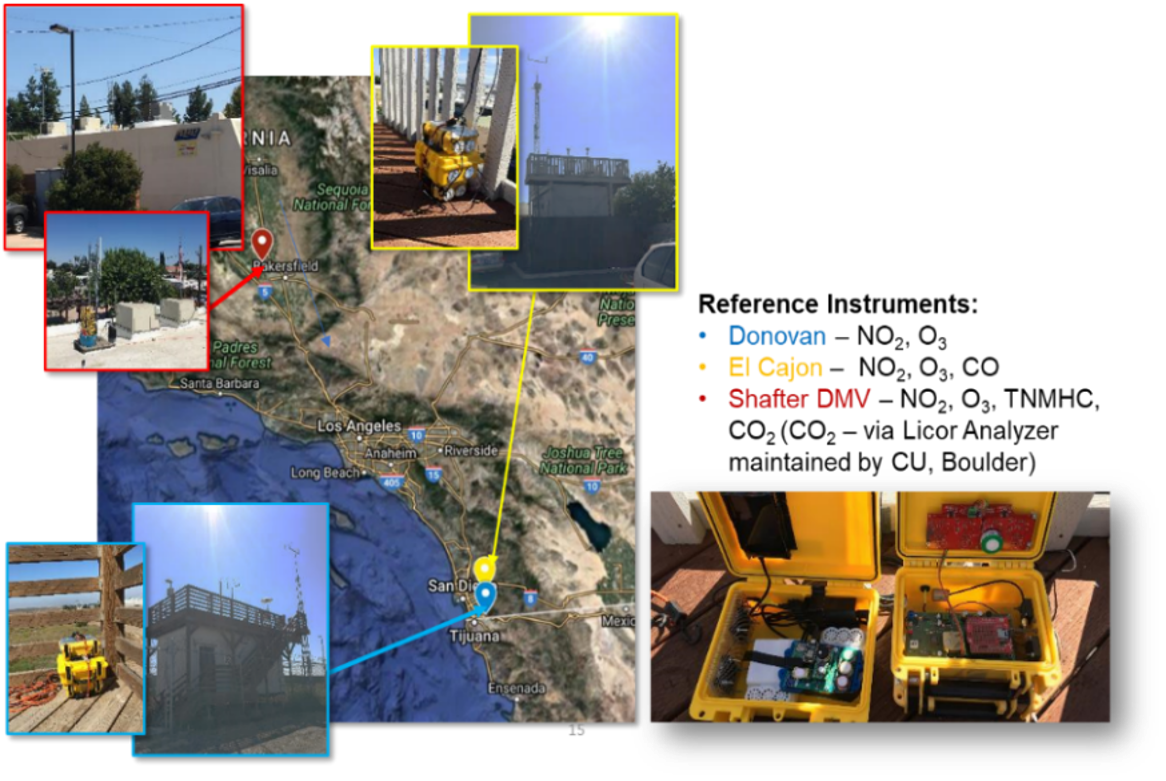
\includegraphics[width=0.75\textwidth]{writeup/img/MSdeployment.png}
\caption{Map and images of deployment locations. Shafter DMV (red) was located 250 mi away from Donovan (blue) and El Cajon (yellow), which were located in San Diego, CA. (bottom right) Deployment containers configuration for the extended deployment. Each container has active ventilation to keep the internal conditions equivalent to the ambient environment.}
\label{fig:img-map}
\end{figure}

For this deployment, we coordinated with three regulatory monitoring sites and rotated sensor packages through each site over the course of approximately six months. Each monitoring site included reference instruments for NO\textus{2} and O\textus{3}, among others. The first site was in El Cajon, CA, in a suburban area east of San Diego, CA near an elementary school and a major highway (El Cajon Site). The second site was directly south 15 miles in the south east corner of San Diego, a more rural area approximately two miles from the border crossing for heavy duty vehicles at Otay Mesa (Donovan Site). The third site was in rural Shafter, CA, 250 miles to the north near Bakersfield.  It is considerably inland compared to the other sites with nearby agriculture as well as oil and gas extraction activities. We expected to see a unique environmental profile (i.e., temperature, humidity, and barometric pressure) at the Shafter site due to being considerably more inland, where weather would be more dominated by the desert ecosystem rather than the ocean ecosystem.  We also expected to see unique emission profiles among the sites.  Donovan was expected to show higher truck emissions due to the presence of heavy duty vehicles, potentially idling for long periods of time, while Shafter was expected to be affected by emissions from its nearby oil and gas activity. We expected the El Cajon site's emissions profile to resemble that of a typical urban/suburban site.  This variety of environmental and emissions profiles would allow us to meaningfully test for transferability, in particular to assess to what degree a calibration model trained on one site would overfit for the other sites.

\subsection{The MetaSense System}

\subsubsection{Hardware Platform}

A low-cost air quality sensing platform was developed to interface with commercially available sensors, initially described in \citet{Chan2017context}. The platform was designed to be mobile, modular, and extensible, enabling end users to configure the platform with sensors suited to their monitoring needs. It interfaces with the Particle Photon or Particle Electron platforms, which contain a 24 MHz ARM Cortex M3 microprocessor and a Wi-Fi or 3G cellular module, respectively. In addition, a Bluetooth Low Energy (BLE) module supports energy efficient communication with smartphones and other hubs with BLE connectivity. The platform can interface with any sensor that communicates using standard communication protocols (i.e. analog, I2C, SPI, UART) and supports an input voltage of 3.3 V or 5.0 V. The platform can communicate results to nearby devices using BLE or directly to the cloud using Wi-Fi or 2G/3G cellular, depending on requirements.  USB is also provided for purposes of debugging, charging, and flashing the firmware.  The firmware can also be flashed or configured over the air. An SD card slot provides the option for storing measurements locally, allowing for completely disconnected and low-power operation.

Our configuration utilized electrochemical sensors for traditional air quality indicators (NO\textus{2}, CO, O\textus{3}), nondispersive infrared sensors for CO\textus{2}, photoionization detectors for volatile organic compounds (VOCs), and a variety of environmental sensors (temperature, humidity, barometric pressure). The electrochemical sensors (NO\textus{2}: Alphasense NO\textus{2}-A43F, O\textus{3}: Alphasense O\textus{3}-A431, and CO: Alphasense CO-A4) are mounted to a companion analog front end (AFE) from Alphasense, which assists with voltage regulation and signal amplification. Each sensing element has two electrodes which give analog outputs for the working electrode (WE) and auxiliary electrodes (AE). The difference in signals is approximately linear with respect to the ambient target gas concentration but have dependencies with temperature, humidity, barometric pressure, and cross-sensitivities with other gases. The electrochemical sensors generate an analog output voltage, which is connected to a pair of analog-to-digital converters (ADCs), specifically the TI ADS1115, and converted into a digital representation of the measured voltage, which is later used as inputs for our machine learning models.

% Electrochemical sensors offer a relatively high level of accuracy at a low current consumption. 

\begin{figure}
\centering
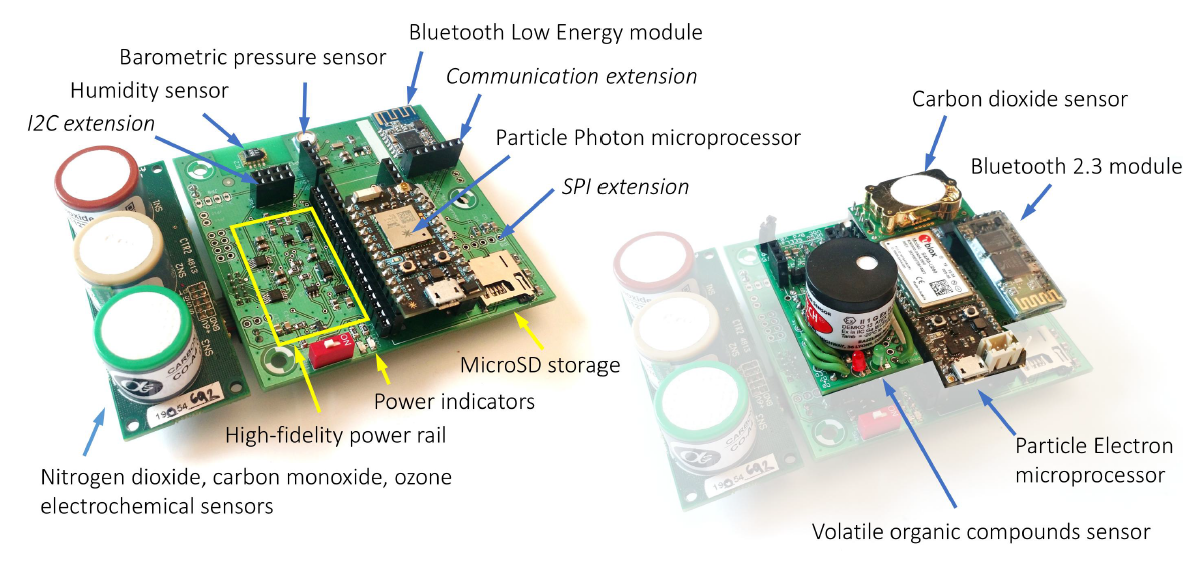
\includegraphics[width=0.75\textwidth]{writeup/img/metasense-platform}
\caption{Labeled MetaSense Air Quality Sensing Platform. (Left) Modular, extensible platform in standard configuration with NO\textus{2}, O\textus{3}, and CO electrochemical sensors. (Right) Additional modules that can be added to the board for additional measurement capabilities.}
\label{fig:img-label}
\end{figure}

Modern low-cost electrochemical sensors offer a low cost and low power method to measure pollutants, but currently available sensors are more optimized for industrial applications than air pollution monitoring: the overall sensing range is too wide and the noise levels are too high. For example, the AlphaSense A4 sensors for NO\textus{2}, O\textus{3}, and CO have a measurement range of 20, 20, and 500 ppm, respectively, which is significantly higher than the unhealthy range proposed by the United States Air Quality Index. Unhealthy levels for NO\textus{2} at 1-hour exposure range from 0.36 – 0.65 ppm, O\textus{3} at 1-hour exposure from 0.17 – 0.20 ppm, and CO at 8-hour exposure from 12.5 – 15.4 ppm (Uniform Air Quality Index (AQI) and Daily Reporting, ~\citeyear{AQI2015}). Along with the high range, the noise levels of the sensors make it difficult to distinguish whether air quality is good. Using the analog front end (AFE) offered by Alphasense, the noise levels for NO\textus{2}, O\textus{3}, and CO have standard deviations of 7.5 ppb, 7.5 ppb, and 10 ppb, respectively. These standard deviations are large compared to observed signal levels for NO\textus{2} and O\textus{3} measurements, which ranged between 0 – 35 ppb and 12 – 60 ppb, respectively, during the 6 month testing period.

The ambient environmental sensors accurately measure temperature, humidity, and pressure and are important for correcting the environmentally related offset in electrochemical sensor readings. The TE Connectivity MS5540C is a barometric pressure sensor capable of measuring across a 10 to 1100 mbar range with 0.1 mbar resolution. Across 0 C to 50 C, the sensor is accurate to within 1 mbar and has a typical drift of +/- 1 mbar per year. The Sensiron SHT11 is a relative humidity sensor capable of measuring across the full range of relative humidity (0 to 100\% RH) with a 0.05\% RH resolution. Both sensors come equipped with temperature sensors with $\pm$0.8 C and $\pm$0.4 C accuracy, respectively. The sensors stabilize to environmental changes in under 30 seconds, which is sufficiently fast to accurately capture changes in the local environment.

In order to improve the robustness of the boards to ambient conditions, the electronics were conformally coated with silicone and placed into an enclosure as shown in Figure~\ref{fig:img-enclosure}. The housing prevents direct contact with the sensors by providing ports over the electrochemical sensors and a vent near the ambient environmental sensors. The system relies on passive diffusion of pollutants into the sensors due to the high power cost of active ventilation.  However, as described in Section~\ref{DataCollection}, for this study the housed sensor packages were placed in an actively ventilated container.

%The passive diffusion model is acceptable for the mobile sensor use case, though, because external movement of the sensor will cause a higher exchange rate of air into the enclosure. 
%WGG: I think it may not be entirely acceptable. :)


\begin{figure}[t]
\centering
\includegraphics[width=0.75\textwidth]{writeup/img/MetaSense_enclosure_outline.png}
\caption{An enclosure was 3D printed for the MetaSense Air Quality Sensing Platform with top-side ports above the electrochemical sensors and a side port next to the ambient environmental sensors.}
\label{fig:img-enclosure}
\end{figure}

\subsubsection{Software Infrastructure}

%We developed the software infrastructure for the MetaSense sensing platform to support multiple usage scenarios. The firmware is configured to support four communication media. A board can communicate via Bluetooth Low Energy (BLE) or USB to a control program that can configure the platform and collect real-time data. The USB connection also supports debugging the board, charging the board, and updating the firmware. Depending on the hardware configuration, Photon or Electron, the MetaSense board can connect directly to the cloud via Wi-Fi or 3G cellular, respectively. These mediums enable over-the-air firmware updates. Each sensor is equipped with an SD card, allowing all readings to be stored locally for redundancy and for deployment situations where energy consumption is critical.

We developed two applications for Android smartphones that leverage the BLE connection of the MetaSense platform. The first application, the MetaSense Configurator app, enables users to configure the hardware for particular deployment scenarios, adjusting aspects such as sensing frequency, power gating of specific sensors connected, and the communication networks utilized.  The second application, simply called the MetaSense app, collects data from the sensor via BLE and uploads all readings to a remote database.  Each sensor reading is stamped with time and location information, supporting data analysis for mobile use cases. Moreover, users can read the current air quality information on their device, giving them immediate and personalized insight into their exposure to pollutants.

% For example, CO\textus{2} and VOC sensor readings can be enabled or disabled by the configuration application. In another example, if the MetaSense sensing platform is being used as a mobile sensor tethered to a smartphone over BLE, users can disable Wi-Fi (or Cellular) radios to save power. 

The remote measurements database is supported by the MetaSense cloud application and built on Amazon's AWS cloud.  Not only can the MetaSense app connect to this cloud, but the MetaSense boards can be configured to connect directly to it using Wi-Fi or 3G.  The measurement data can be processed by machine learning algorithms in virtual machines in AWS or the data can be downloaded to be analyzed offline.  The aforementioned over-the-air firmware updates are handled through Particle's cloud, which also allows remotely monitoring, configuring and resetting boards. These direct-to-cloud features are key to supporting a long-term, wide-scale deployment like the one presented in this paper.

\subsection{Data Collection and Preprocessing}
\label{DataCollection}
To support a long-term deployment in potentially harsh conditions, the sensors were placed into environmentally robust containers, shown in Figure~\ref{fig:img-map}, bottom right. The container was a dry box, measuring 27.4 x 25.1 x 12.4 cm, that was machined to have two sets of two vents on opposing walls. Louvers were installed with two 5 V, 50 mm square axial fans expelling ambient air from one wall and two louvers allowing air to enter the opposite side. The configuration allowed the robust container to equilibrate with the local environment for accurate measurement.  Each container could hold up to three MetaSense boards with cases and complementary hardware.  Due to the long timeframe of the deployment, a USB charging hub was installed into the container to power the fans, the air quality sensors, and either a BLU Android phone or Wi-Fi cellular hotspot. The phones and hot spots were used to connect the sensors to the cloud; therefore, we could remotely monitor the sensors’ status in real-time and perform preliminary data analysis and storage. Each board also had an SD card to record all measurements locally, increasing the reliability of data storage. 

Each container holding three MetaSense sensor packages was placed at one of three sites for simultaneous data collection across the sites. After a period of time the containers were rotated to a new site such that every package spent a period of time at every site.  We performed three rotations such that every sensor was returned to its original site for the final collection, but we disregarded the data from the initial round 0, except to verify that sensor performance had not changed measurably between the beginning and the end of the deployments. \autoref{tab:board-rotations} lists the dates for each rotation as well as where each sensor system was located for each rotation.  The dates are approximate due to the logistics of gaining access to regulatory field sites and the distances traveled to deploy sensors.  Also of note is that the deployments are not of equal length.  This does not affect the results reported below because we ran all combinations of training and testing sites, and training set sizes were normalized to remove the influence of training set size. The data from the reference monitors was provided by the cooperating air quality districts in the form of minute-averaged O\textus{3} and NO\textus{2} concentrations for the time period that our sensor packages were deployed.

\begin{table}[t]
\centering
\caption{Board locations and dates for each round.}
\begin{tabular}{l|llll}
                  & \textbf{Round 1} &            \textbf{Round 2} &                   \textbf{Round 3} \\
         & \textbf{9/26/17 - 10/19/17} & \textbf{10/19/17 - 12/21/17} & \textbf{12/21/17 - 3/5/18} \\ \hline
\textbf{Board 17} & El Cajon    & Shafter      & Donovan    \\
\textbf{Board 19} &  El Cajon    & Shafter     & Donovan   \\
\textbf{Board 21} &  El Cajon    & Shafter     & Donovan  \\ \hline
\textbf{Board 11} &  Shafter      & Donovan  & El Cajon  \\
\textbf{Board 12} &  Shafter      & Donovan  & El Cajon  \\
\textbf{Board 13} &  Shafter      & Donovan  & El Cajon  \\ \hline
\textbf{Board 15} &  Donovan   & El Cajon   & Shafter    \\
\textbf{Board 18} &  Donovan   & El Cajon   & Shafter     \\
\textbf{Board 20} &  Donovan   & El Cajon   & Shafter   
\end{tabular}
\label{tab:board-rotations}
\end{table}

Prior to using the dataset for training the calibration models, we performed a preprocessing step. First, we programmatically filtered out data samples that contained anomalous values that might have occurred due to a temporary sensor board malfunction (e.g., due to condensation).  Specifically, we searched for temperature and voltage spikes that were outside the realm of reasonable values (i.e., temperature values above 60 degrees Celsius or ADC readings above 5 volts) and removed the corresponding measurements.  Each removed sample was visually inspected to ensure data was not being erroneously removed. The remaining data was averaged over a minute window to match the time resolution of the data from the reference monitors.  Although we gathered sensor voltage measurements from both the auxilliary ($AE$) and working electrodes ($WE$) of the electrochemical sensors, we used the difference between the two ($AE - WE$) as the representative voltage for each sensor since the auxilliary voltage is meant to serve as a reference voltage for the working electrode. This treatment is consistent with the methodology of \citet{Zimmerman2018}, and we validated that the performance of the calibration models did not differ between tests with both electrodes and test with the difference as input features. The resulting data set over the three rounds at the three site contains 1,200,000 minute-averaged measurements.

With this data, we were able to verify our claim in Section \ref{SamplingSites} that we would observe varied environmental and pollutant conditions among the sites. Generally higher ozone values were reported at Shafter, whereas generally higher NO\textus{2} values were reported at Donovan.  Higher humidity values were reported at the Donovan and El Cajon sites, as compared to Shafter.  Some of the lowest temperature values were reported at Shafter.  For more information see the distribution plots in Appendix \ref{Distributions}. 

\subsection{Baseline Calibration Methods}\label{sec:calibration-methods}
Sensor calibration is the process of developing and training models to convert a sensor voltage into a pollutant concentration. We formulate sensor calibration as a regression problem with input features $x$ and $e$ representing signals from the electrochemical sensors (O\textus{3} voltage, NO\textus{2} voltage, CO voltage) and environmental factors (temperature, pressure, humidity), respectively, for a total of 6 features. These features are input to a calibration function $h_\theta(x, e)$ that estimates target values $y$ representing pollutant concentrations (O\textus{3} ppb and NO\textus{2} ppb). 

In our regression problem, we seek a function such that $h_\theta(x, e) \approx y$, which we formulate as an optimization where we minimize error over a training data set $\{x_n, e_n, y_n\}_{n = 1}^N$ according to a loss function $L(h_\theta(x, e), y)$, i.e. 
\begin{equation}
\theta^* = \argmin_\theta \frac{1}{N}\sum_{n = 1}^N L(h_\theta(x_n, e_n), y_n)
\end{equation}
Models trained in this way assume that at inference time, predictions are made on data sampled from the training distribution. While this assumption holds true when the air quality sensors are trained and tested at the same site, the distribution of pollutants and environmental conditions changes when the sensors are moved to a new location. 

We investigated the performance of three calibration models: multiple linear regression, neural networks (sometimes called deep learning), and random forest.  These methods vary in their ability to accurately model complex behaviors, otherwise known as \textit{capacity}, with linear regression having relatively low capacity and neural nets and random forests having substantial capacity.  The price of high capacity is the potential to overfit the training distribution, which is a failure to generalize beyond the training data. Models that overfit will incur significant error when predicting on out-of-distribution examples. Overfitting can be mitigated with regularization and by reducing the model capacity, but this can only go so far if the testing distribution is substantially different from the train distribution. All of these methods have been previously applied to ambient pollutant estimation by various research groups \citep{Piedrahita2014,Spinelle2015,SPINELLE2017706,Sadighi2018,Zimmerman2018,Casey2018testing} and are generally common predictive modeling methods.  For neural nets, we investigated three variants: two-layer, four-layer, and four-layer with a "split" architecture, which we motivate and describe in the next subsection.

%The MetaSense project is concerned with deploying mobile, portable sensors and thus we wish to train calibration models that can generalize beyond the data obtained via colocation. As previously described, we colocated MetaSense boards with EPA stations across three locations in California (El Cajon, Donovan, Shafter). By training a calibration model on training data restricted to some sites and testing on the other site, we measure how well particular models generalize to different locations.

Our baseline models were trained using the Scikit-Learn Python package, and the model parameters for each baseline model can be seen below:
\begin{enumerate}
    \item \textbf{Linear regression:} we assume the functional form $h(x) \triangleq w^T x + b$, and fit the parameters in closed form. We use no regularization or polynomial features.
    \item \textbf{Two-layer neural network:} we fit a two-hidden layer (200 wide) multilayer perceptron with rectified-linear unit activation functions and a final linear layer. We train this neural network using the Adam optimizer ($\beta_0 = 0.9, \beta_1 = 0.999$) and a learning rate of $10^{-3}$.
    \item \textbf{Four-layer neural network:} Same as two-layer neural network, but four hidden layers of width 200 instead of two.
    \item \textbf{Random forest:} We divide our data into five folds and train a random forest of size 100 on each fold, resulting in 500 trees. We aim to reproduce the strategy of \cite{Zimmerman2018} as closely as possible.
\end{enumerate}

\iffalse
\begin{align*}
    \mathrm{MAE}(h(x), y) &= |h(x) - y| \\
    \mathrm{CvMAE}(h(x), y) &= \frac{1}{\textrm{Average conc. of pollutant}}|h(x) - y| \\
\end{align*}
\fi

\subsection{Split Neural Network Method}\label{sec:split-nn}
Overfitting is a problem for high capacity models with a limited distribution in training data, resulting in poor performance when a model is transferred to new locations and environments. One method to improve model transferability would be to collect more training data that includes the test distribution. However, colocating a sensor at multiple different regulatory field sites in order to capture a sufficiently wide distribution is prohibitive in terms of cost and time.  An alternative solution is to deploy a set of sensors based on the same technology across multiple sites and then pool their data.  However, there can be substantial sensor-to-sensor variance in performance that would amplify prediction errors.  We propose a training architecture that consists of two sets of models: a global calibration model that leverages the data from a set of similar sensors spread across different training environments and sensor-specific calibration models that detect and correct the error between sensors.

In the previous subsection, we associated each board $i$ with a calibration function $h_{\theta_i}(x)$ and fit this calibration function with its colocated data. Now, consider a collection of many air quality sensors. We propose using a calibration function split into two distinct steps: first, pollutant sensor voltages $x$ are input into a sensor-specific model, $s_{\theta_i}(x)$, a function parameterized by $\theta_i$, which outputs a fixed dimensional vector $u$~\citep{Goodfellow-et-al-2016}. This intermediate representation $u$ is concatenated with environmental data $e$, which is then passed into a global calibration model $c_\phi([u | e])$. For a single air quality sensor, our final calibration function is $c_\phi([s_{\theta_i}(x) | e])$.  Figure~\ref{fig:split-nn-deploy} depicts the use of such a model.  Such a model is called a split neural network model (\textit{split-NN}) since neural networks are generally used for both the sensor-specific models and the global calibration models. In our experiments, the sensor-specific model $s_{\theta_i}$ is either a linear regressor or neural network  and $c_\phi$ is a two-layer, 100-wide neural network. 

The purpose of the split-NN model is that $s_{\theta_i}$ corrects for differences in air quality sensor $i$'s performance relative to the other sensors, thus normalizing the values and making the behavior of all the sensors compatible with the global model $c_\phi$.  The performance of the estimates from $c_\phi$ should be superior to those from an individual sensor model because it been trained on the (normalized) data of all the boards as opposed to just a single board.

\begin{figure}
    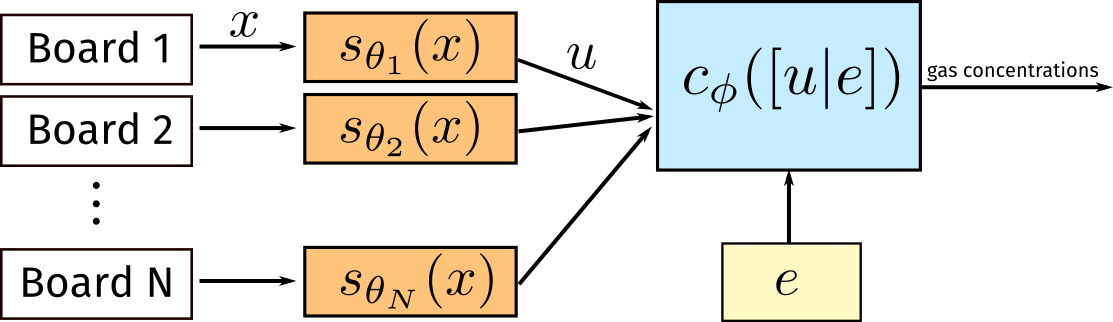
\includegraphics[width=0.8\textwidth]{writeup/img/split-model.png}
    \caption{Architecture of the split-NN model in deployment (testing).  Each air quality sensor has its own custom $s_{\theta_i}(x)$ that is intended to take the sensor's output ($x$) and normalize it ($u$) relative to the other sensors, so that it can be fed into the global model $c_\phi$.}
    \label{fig:split-nn-deploy}
    \todo{WGG: not clear that Board 2 - Board N should be in this figure.  Maybe grayed out?  No additional subscripts needed.}
\end{figure}

The split model can be trained efficiently with stochastic gradient descent. Specifically, we first collect $N$ data sets for each board $D_i = \{x^{(i)}, e^{(i)}, y^{(i)}\}_{i = 1}^N$. We ensure each of these data sets is the same size by sampling each with replacement to artificially match the largest data set. We then pool the data sets together into one data set from which we sample mini-batches. While each sensor-specific model $s_{\theta_i}$ is trained only on data collected by its sensor, the regression with the other $s_{\theta_i}$ sensor-specific models is designed to detect and correct its bias, outputting an intermediate representations $u$ that is normalized with the others.  The global calibration model is trained on the normalized data from all air quality sensors.

%\todo{WGG: word choice on the above: optimization, NN loss function contains loss terms from every single board, the optimal performance will happen when they report the same things when they measure the same things} 

Although training this neural network will take longer than training one for a single board, it has several key advantages over conventional calibration techniques. The first is its ability to share information across multiple boards. Suppose Board A is trained on Location 1 and Board B is trained on Location 2. Pooling the data sets and using a shared model enables the global calibration model to predict well in both locations, and the calibration models for both boards will have information about the other locations in them, in theory improving transferability. The second is more efficient utilization of data. By pooling data and training jointly, we effectively multiply our data size by the number of boards.  Alternatively, field deployments can be shortened.

\textbf{Calibrating a New Board without a Full Training.}  Field calibration is traditionally performed by colocating a sensor package with reference monitors and then training to match pollutant concentrations.  But, suppose we already had a fleet of low-cost sensor packages already deployed.  A simpler method not requiring coordination with regulatory agencies would be to colocate it with a calibrated sensor package and train a model to match its predicted pollutant levels. This risks compounding errors across models, however. 

The split-NN model enables calibrating a new sensor package by colocating to match \textit{representation} instead of predictions~\citep{Goodfellow-et-al-2016}.  We propose calibrating sensor package $N+1$ to match the intermediate representation output of a colocated, previously-calibrated sensor package. Specifically, we train model $N + 1$ to minimize $L(u_N, u_{N + 1})$, or the loss between the two packages' intermediary outputs. These intermediate representations are designed to be robust to changes in location so training to match these representation so it is expected that it will result in a robust calibration model. We analyze this potential calibration technique by holding out a board from our data sets and training a split model. We then simulate calibrating the held out board by training a sensor model to match the representations produced by another board it was colocated with. We then use this new sensor model with the global calibration function to produce pollutant values. 

%The split-NN offers a novel method to calibrate new boards. Suppose we have a set of $N$ calibrated boards and are presented with an uncalibrated $N + 1$-th board. The safest way to calibrate this new board would is always to colocate it with a ground-truth sensor and train a model.  This requirement, however, is potentially restrictive and expensive, as it necessitates deploying the sensor by an EPA or other reliable sensor. On the other hand, colocating with another low cost sensor is simple and cheap, but risks compounding the noise and error that already exist.

\section{Results and Discussion}

\subsection{Robustness of Different Calibration Techniques Across New Locations}
We evaluated a set of four baseline models described in Section~\ref{sec:calibration-methods}: multiple linear regression, two-layer neural network (NN-2), four-layer neural network (NN-4), and random forest (RF). With each of these four models, we performed a suite of identical calibration benchmarks that measure the robustness of models to out-of-distribution data. We split all data sets uniformly at random into training and testing subsets, reserving 20\% of each board's data for testing.  In each benchmark, we progressively widened the training distribution by combining training data from more locations (using subsampling to maintain the training set size), while keeping the testing set data set from one location.  We have four ``levels'' of such benchmarks:
\begin{itemize}
    \item \textbf{Level 0:} Train a model on one location and test on the same location.  Several studies, discussed in Section \ref{Introduction}, have previously assessed this configuration \citep{Zimmerman2018,Spinelle2015,SPINELLE2017706,Cross2017}.
    \item \textbf{Level 1:} Train a model on one location and test on another location.  Some recent studies, also discussed in Section \ref{Introduction}, have previously studied this configuration \citep{Hagan2018, Casey2018testing, Bigi2018performance, Malings2018Development}.
    \item \textbf{Level 2:} Train a model on two locations and test on a third location.
    \item \textbf{Level 3:} Train a model on three locations and test on one of the three locations.
\end{itemize}
\begin{figure}
\begin{subfigure}{0.23\textwidth}
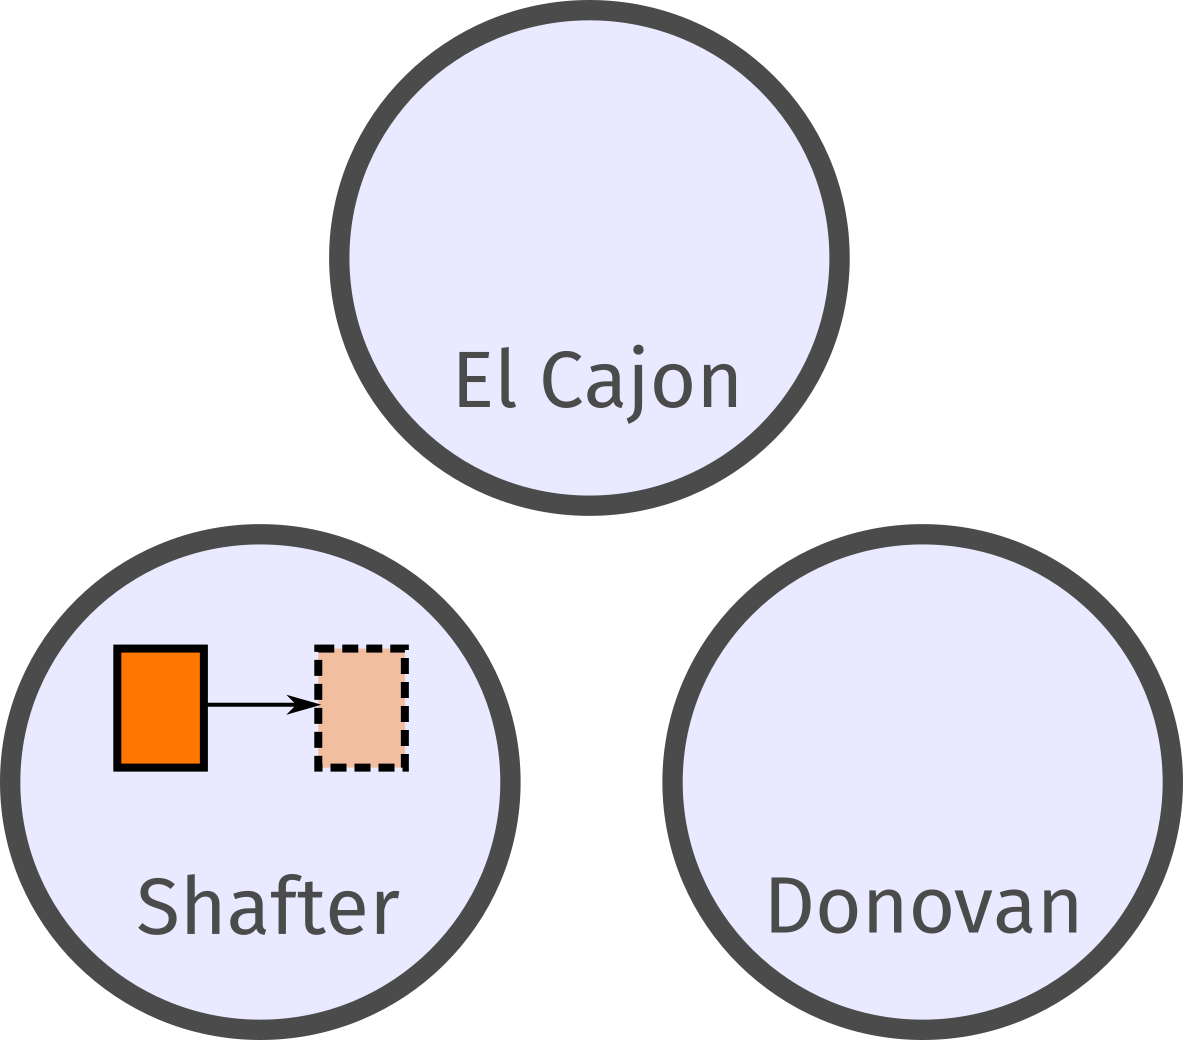
\includegraphics[width=\textwidth]{writeup/img/level0.png}
\caption{Level 0}
\end{subfigure}
~
\begin{subfigure}{0.23\textwidth}
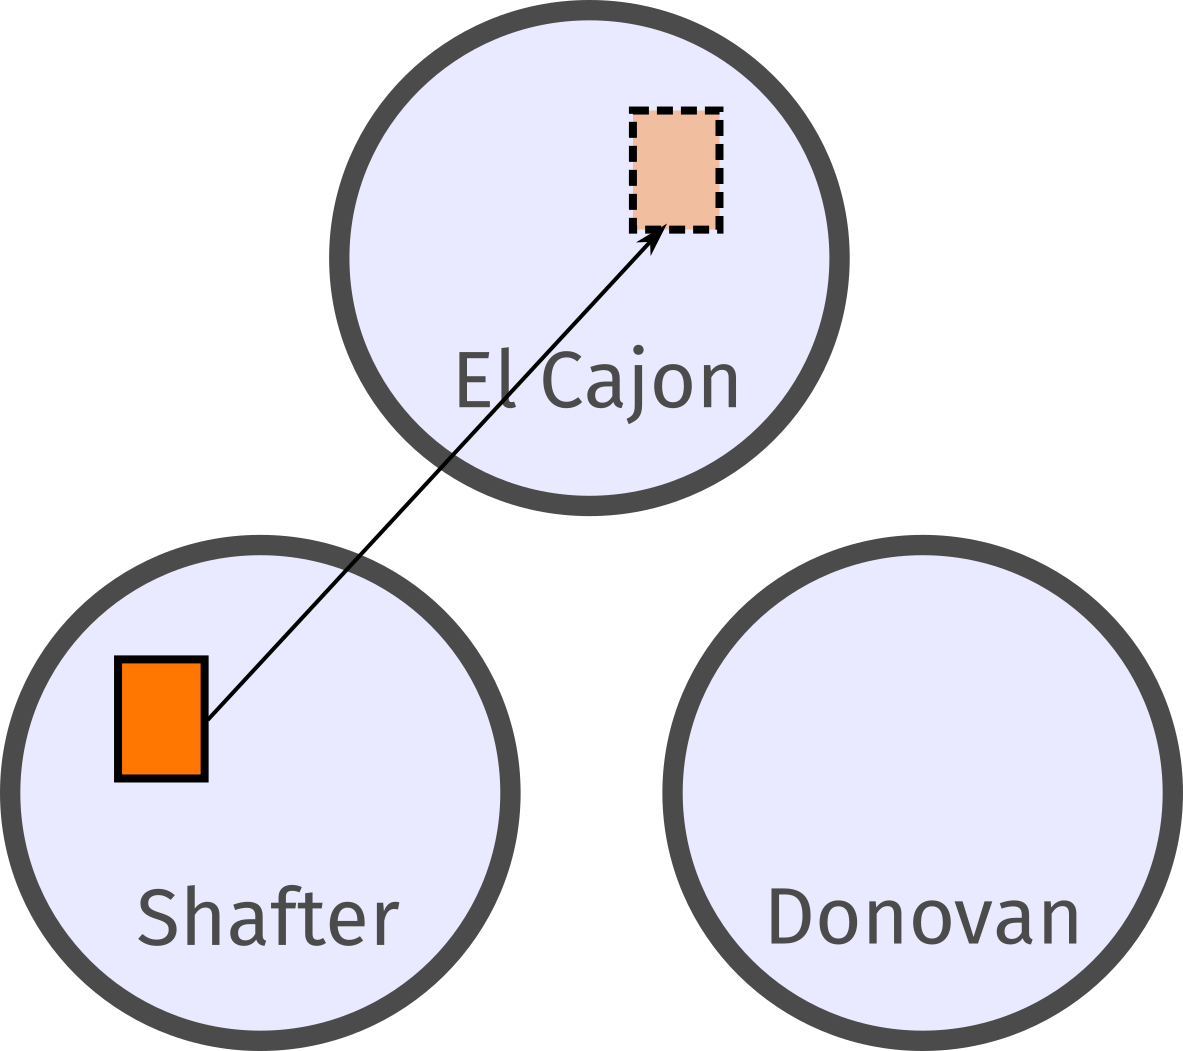
\includegraphics[width=\textwidth]{writeup/img/level1.png}
\caption{Level 1}
\end{subfigure}
~
\begin{subfigure}{0.23\textwidth}
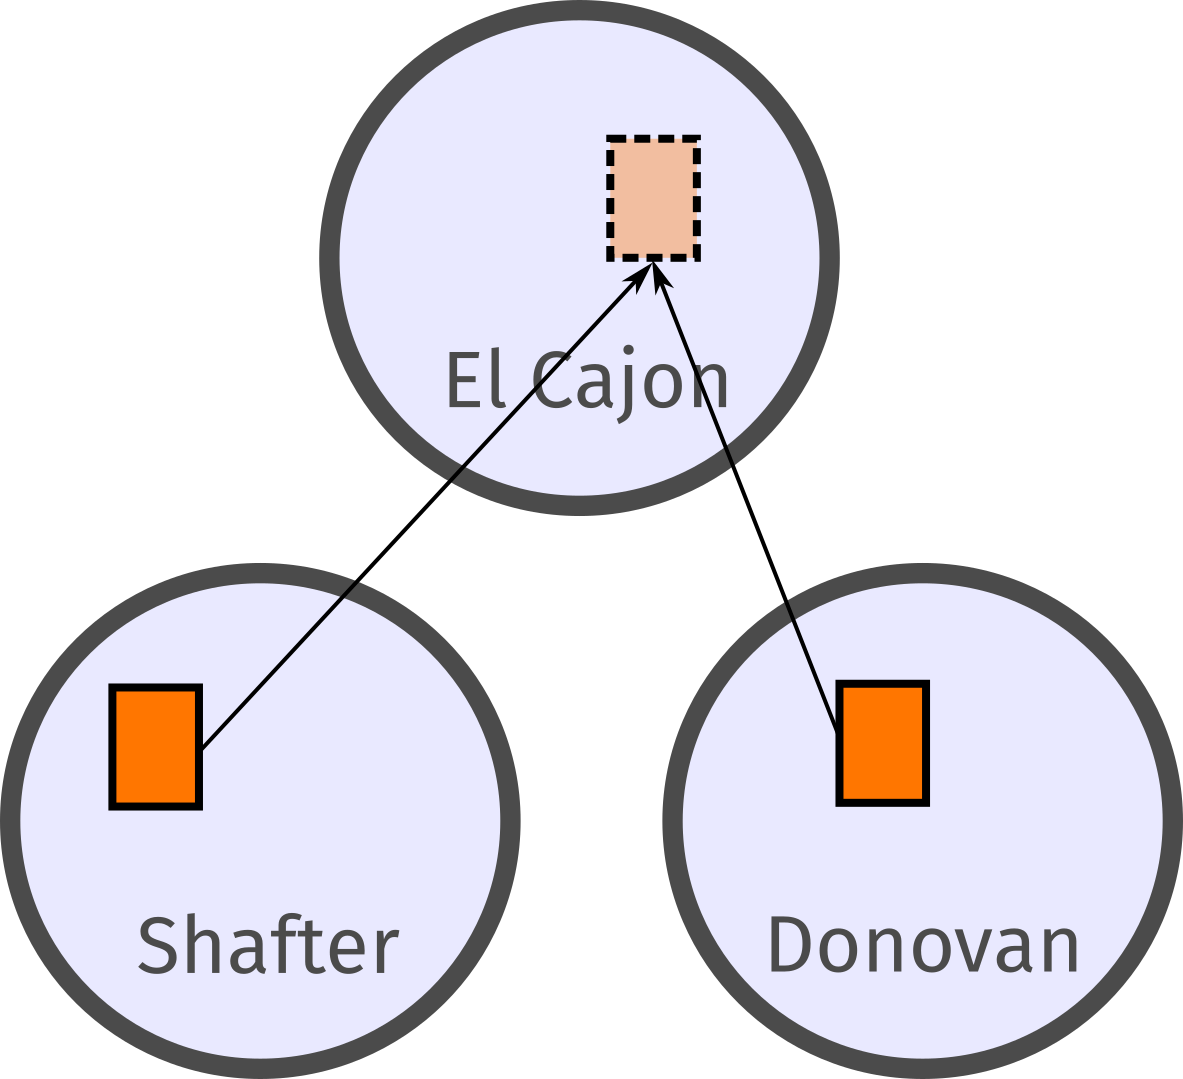
\includegraphics[width=\textwidth]{writeup/img/level2.png}
\caption{Level 2}
\end{subfigure}
~
\begin{subfigure}{0.23\textwidth}
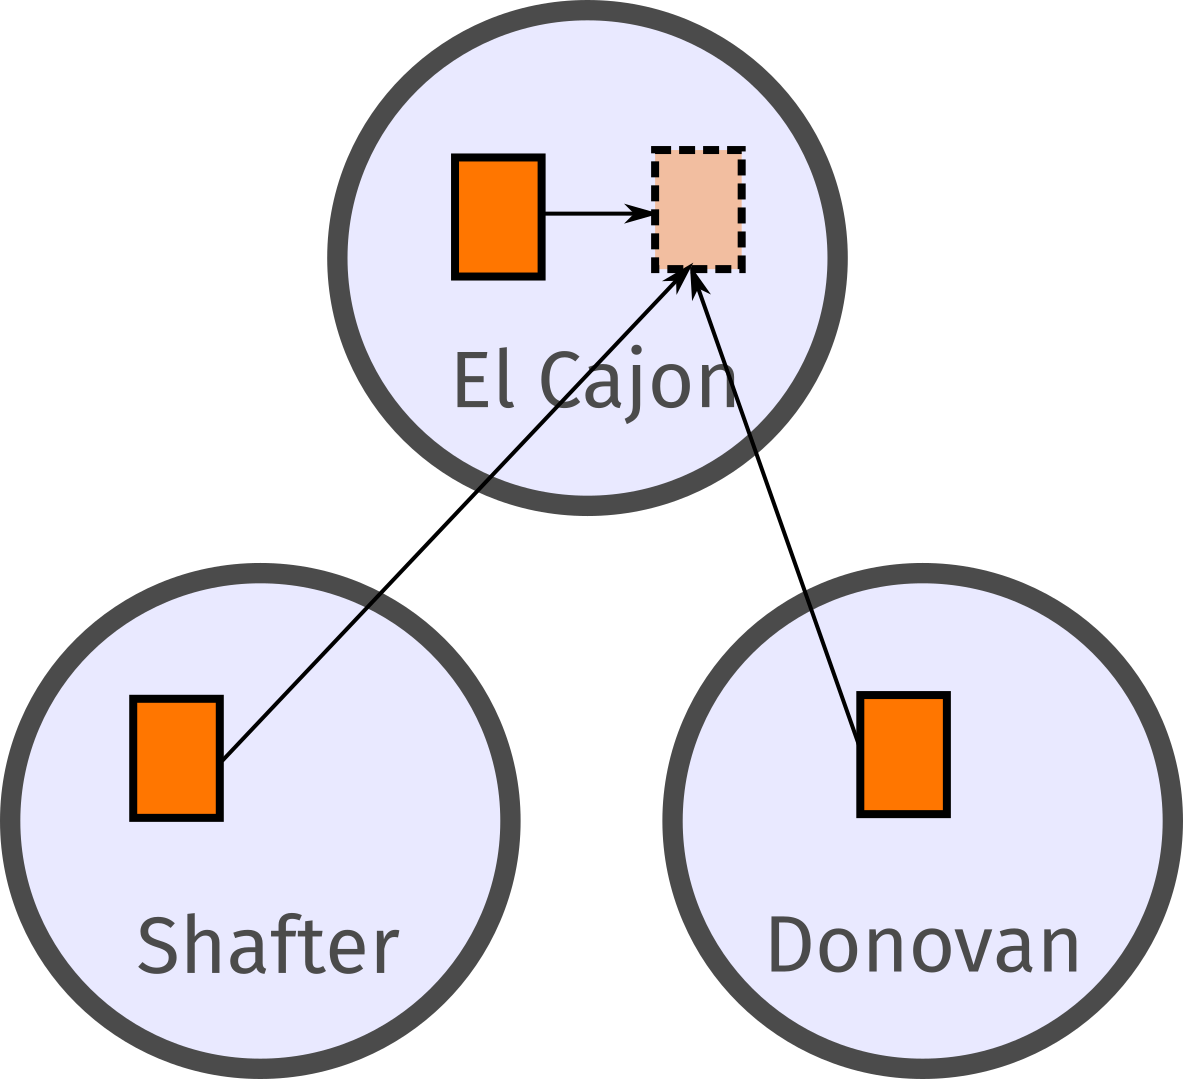
\includegraphics[width=\textwidth]{writeup/img/level3.png}
\caption{Level 3}
\end{subfigure}
\caption{Graphical depiction of training versus testing for the Level 0 through Level 3 benchmarks.  The Level 0 and 3 benchmarks test on a training site using held out data.  The Level 1 and 2 benchmarks train and test on different sites, also using held out data for consistency.}
\end{figure}

In the Level 0 and Level 3 benchmarks, the training and testing data distributions have explicit overlap, whereas in Level 1 and 2, there is no explicit overlap. We expect performance on Level 0 to be the best, as the training and testing distributions are identical.  We expect performance on Level 3 to be similar, due to the overlap in training and testing distributions. We expect performance on Level 1 to be the worst, as the training distribution is the narrowest and with no explicit overlap, whereas we expect performance on Level 2 to be between Level 1 and Level 3, for although there is no explicit overlap, the overall training distribution will be wider, forcing the models to be more general and possibly affording more implicit overlap.  Furthermore, we expect higher capacity models to overfit more to the training data set, and as a result, have the largest gap between Level 0 and Level 1. Thus, we expect linear regression to have more consistent performance across the benchmarks, albeit at relatively high error, followed by the 2-layer neural network, 4-layer neural network, and finally the random forest.

We ran each benchmark across all possible permutations of location and sensor package, measuring six metrics: root mean squared error (rMSE), centered root mean squared error (crMSE), mean absolute error (MAE), the coefficient of variation of mean absolute error (CvMAE), mean bias error (MBE), and coefficient of determination ($R^2$). The results for MAE of the baseline models are plotted in Figure~\ref{fig:results-linear}.  Details can be explored further in Table~\ref{fig:six-errors-table} in Appendix~\ref{app:six-errors}.

\begin{figure}[t]
\centering
\begin{subfigure}{0.45\textwidth}
\includegraphics[width=\textwidth]{\baselinedir/NO2" "MAE_test.png}
\caption{NO\textus{2}}
\end{subfigure}
\begin{subfigure}{0.45\textwidth}
\includegraphics[width=\textwidth]{\baselinedir/O3" "MAE_test.png}
\caption{O\textus{3}}
\end{subfigure}
\caption{Mean absolute error (MAE) boxplots for NO\textus{2} and O\textus{3}, for the Level 0 through Level 3 benchmarks.}
\label{fig:results-linear}
\end{figure}

We observe that on average, as model capacity increases, Level 0 error decreases. This is consistent across both NO\textus{2} and O\textus{3} prediction and reflects the ability of the model to fit the training distribution. Concerning model transferability, we find that consistently, \emph{all models suffer significant error when tested on different locations}. Level 1 and 2 benchmarks reflect the ability of a model to generalize to a distribution it hasn't seen before and we see that in these benchmarks, errors are much higher and the gaps between models are much smaller. Furthermore, Level 2 error is slightly lower on average than Level 1 error. By adding data from another site, effectively widening the training distribution, the models are slightly more robust to the unseen testing distribution. Level 3 performance aligns closely with Level 0 performance, which is to be expected, since in both cases the training distribution contains the testing distribution.

Across baselines, we observe that on average, linear regression has the highest error on all the benchmarks. However, its errors across the Level benchmarks are more consistent than the other models, suggesting that low-capacity linear regression is more robust to transfer. On the other hand, random forests have on average the lowest error, but have the most inconsistent results across the Levels. The results indicate a tradeoff between model capacity and robustness to transfer, consistent with our intuitions about model overfitting and generalization. Neural networks lie in between linear regression and random forests, and offer a tradeoff between low error and consistent error. 

\iffalse

\begin{itemize}
    \item  \emph{Current techniques assume that the conditions of sensor use match those of calibration.  How reasonable are these assumptions in practice?}
    \begin{itemize}
        \item Summarize the results of training on one location and testing on the others, compare the results across MLR, NN, and RF 
        \item Discuss the implications of these results, what does it mean for groups that are calibrating sensors in one location in a city and then moving them to new locations? Or groups calibrating in one city and deploying in another city? Is the drop in performance worse for moving sensors to a new city versus a new location in the same city (this could be valuable information for other researchers and regulatory agencies) Also, out of the quantification techniques tested (MLR, NN, RF) which would be recommended for different situations?
    \end{itemize}
    \item When they fail, what are the underlying causes of those failures?  (E.g., variance in humidity, temperature, barometric pressure, or background pollutants.)
    \begin{itemize}
        \item When we have a drop in performance is there still any valuable information in the data (i.e., are the trends still there, is it simply a shift causing the poorer performance?) -> a time series of training data from one San Diego site and that same model tested at the other San Diego site and the Shafter site could help us figure this out. (plot model tested on other site)
        \item Can these drops in performance be attributed to mainly a change in environmental and pollutant distributions between sites OR do different overall/background compositions at sites (based on environmental differences, different sources near and far, etc.) play a large role.
        \item different data distribution
        \item overfitting to environment experiments
        \item include data about RF leaves
    \end{itemize}
\end{itemize}
\fi


\begin{figure}[t]
\centering
\begin{subfigure}{0.33\textwidth}
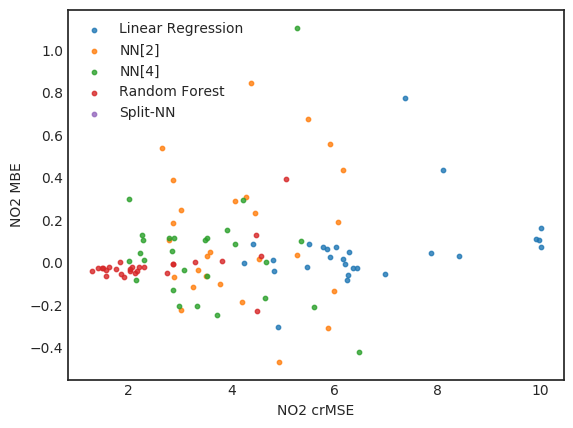
\includegraphics[width=\textwidth]{\baselinedir/NO2_level0_test_target.png}
\caption{Level 0 (NO\textus{2})}
\end{subfigure}
\begin{subfigure}{0.33\textwidth}
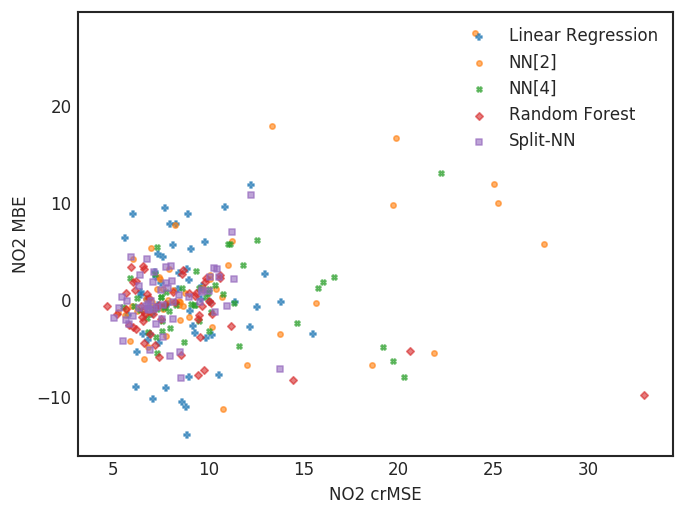
\includegraphics[width=\textwidth]{\baselinedir/NO2_level1_test_target.png}
\caption{Level 1 (NO\textus{2})}
\end{subfigure}
\begin{subfigure}{0.33\textwidth}
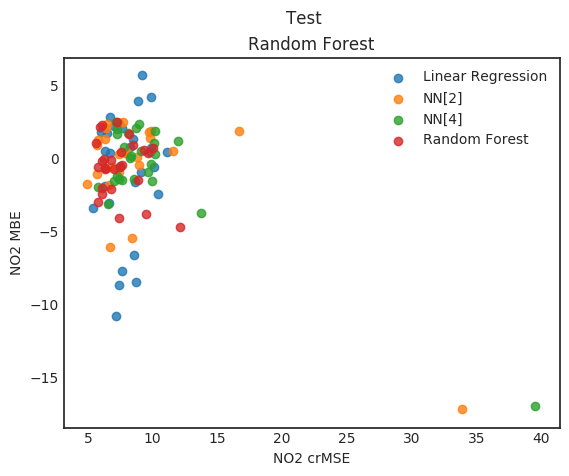
\includegraphics[width=\textwidth]{\baselinedir/NO2_level2_test_target.png}
\caption{Level 2 (NO\textus{2})}
\end{subfigure}
\begin{subfigure}{0.33\textwidth}
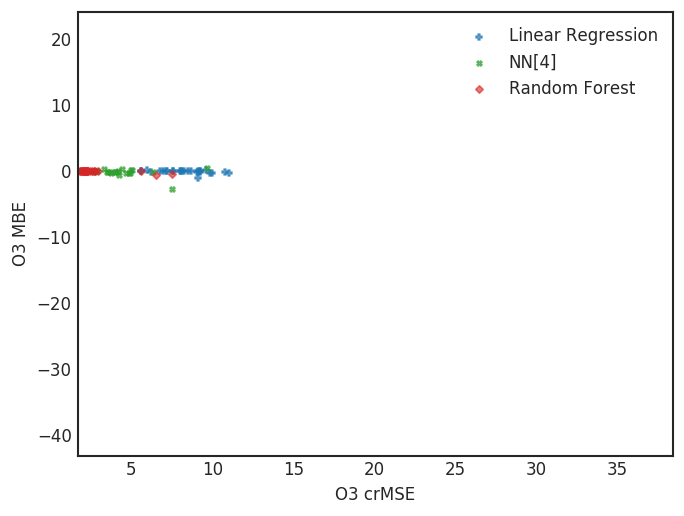
\includegraphics[width=\textwidth]{\baselinedir/O3_level0_test_target.png}
\caption{Level 0 (O\textus{3})}
\end{subfigure}
\begin{subfigure}{0.33\textwidth}
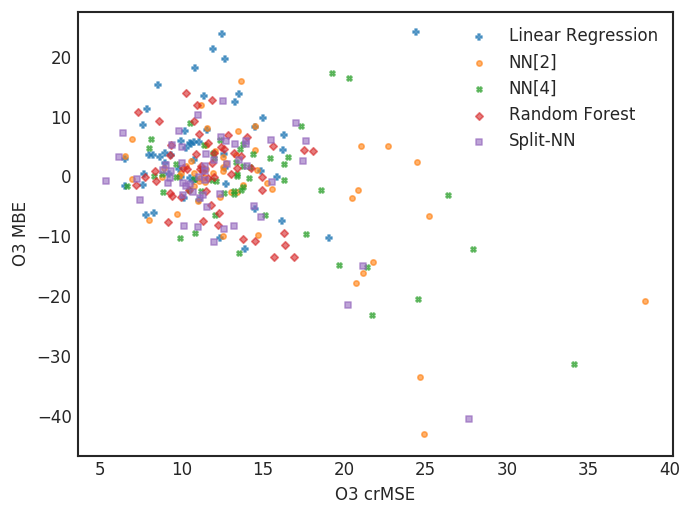
\includegraphics[width=\textwidth]{\baselinedir/O3_level1_test_target.png}
\caption{Level 1 (O\textus{3})}
\end{subfigure}
\begin{subfigure}{0.33\textwidth}
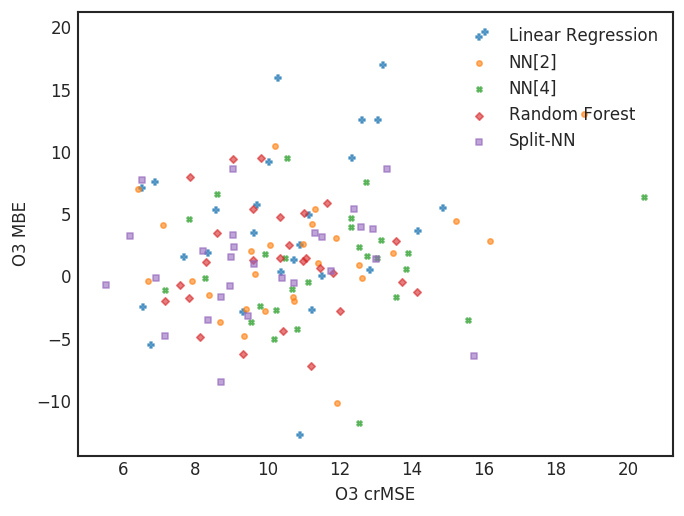
\includegraphics[width=\textwidth]{\baselinedir/O3_level2_test_target.png}
\caption{Level 2 (O\textus{3})}
\end{subfigure}
\caption{Target plots for Level 0 through Level 2 for both NO\textus{2} and O\textus{3}.}
\label{fig:target-plots-levels}
\end{figure}

To better understand how model performance degrades, we produced target plots, which visualize the tradeoff between centered error and bias  error (Figure~\ref{fig:target-plots-levels}).  The target plots indicate that while error approximately doubles when there is no explicit overlap in the distribution, model bias is many times larger. The increase in bias is more pronounced in the higher capacity models. Furthermore, despite the higher capacity models showing better error and bias in a Level 0 benchmark, the models have very similar error-bias tradeoffs in a Level 1 benchmark, indicating that even a high-capacity model cannot avoid this performance degradation.  Finally, in comparing the Level 1 and Level 2 plots, we observe that adding an additional (no-overlapping) site primarily reduces bias.  The Level 3 plots were very similar to the Level 0 plots and were excluded from Figure~\ref{fig:target-plots-levels} for brevity.

In general, however, we observe that model performance degrades non-trivially
when moved to different locations. This decrease in performance could result in overconfidence in a sensor's readings, potentially affecting downstream decisions. We briefly analyze the properties of our data that could result in overfitting by first investigating how data distributions across sites and times differ. Over each location and round, pollutant values can be highly variable. This is reflected, for example, in \autoref{fig:no2-rounds} where Shafter has higher values of NO\textus{2} in Round 1 and 2 but lower in Round 3. Furthermore, in \autoref{fig:o3-rounds}, the distribution of O\textus{3} changes remarkably across round and location. Similarly, temperature and humidity change significantly across location and round, which can be seen in \autoref{fig:temperature-rounds} and \autoref{fig:humidity-rounds}.

%\todo{(in the above, perhaps add something like: the model is overfitting to ambient environmental conditions and not the sensor reading. Many pollutants change with the diurnal cycle of the earth (eg. NO\textus{2} turning into O\textus{3} only when there is UV light, so NO\textus{2} is bigger at night, which is typically cooler and more/less humidity).)}.

A question that remains is to what degree overfitting or unique (non-overlapping) distributions of environmental data at the sites is contributing to the failure of the high capacity models to transfer well.  In an effort to better understand what may be driving the drop in performance of the high capacity models when boards are moved, we examined error density plots for temperature and humidity for the Level 1 benchmarks. In these types of plots, one of the predictors, such as temperature or humidity, is plotted against the error for all three sites in a single plot.  Figure~\ref{fig:error-density} displays the error density plots for absolute humidity against the error for the O\textus{3} estimation, for both the linear regression and random forest models (See the remaining plots in Appendix~\ref{sec:remaining-error-density-plots}). These plots illustrate how the magnitude of error varies with respect to higher or lower predictor values as well as how different pairs of training and testing sites compare. There are a couple of things we can derive from this collection of plots.  First, we observe that the pollutant concentrations at the Shafter site are difficult to predict, except for random forest when trained at Shafter itself (Figure~\ref{fig:error-density}f). The Shafter site was spatially far from the other sites and likely had a unique composition of background pollutants and ambient environmental conditions.  Second, we observe that when training a random forest model at one site and testing it at a different site (Figure \ref{fig:error-density}, bottom row), the error density plots look similar to the results from the linear regression models (Figure \ref{fig:error-density}, top row) despite the higher capacity of random forest models.  We observe that the greater errors at the Shafter site are occurring at humidity values that were seen in the training data set (more centrally in the plot), as is evident by their representation in the Donovan data. This implies that these errors did not occur at humidity values that have been extrapolated beyond the original training data set, but rather from overfitting at values in the distribution.  This leads us to conclude that overfitting is the reason random forest's net performance in transfer is not much better than linear regression.

%For example, in Figures~\ref{fig:error-density}a-c show all combinations of train and test for linear regression.  We note the overall similarity of these three combinations.  The one anomaly that we observe is that the model trained at the Donovan site performs particularly poorly at the Shafter site.  

%training occurs at the Donovan site and the error density pattern seen at the testing site in nearby El Cajon, is fairly comparable.  However, at the second testing site, Shafter, the error is greater. Furthermore, the greater error at the Shafter site is occurring at humidity values that were seen in the training data set (more centrally in the plot), as is evident by their representation in the Donovan data. In other words, these are not humidity values that have been extrapolated beyond the original training data set. The same pattern holds true for temperature (See Appendix~\ref{fig:remaining-error-density-plots} for details): there are greater errors occurring at Shafter as opposed to El Cajon and at least a portion of these errors are not occurring at temperature values that were unseen during training. Thus, if the poorer performance by the linear model in Shafter is not attributable to environmental conditions that the model was simply not trained for, then there must be another factor driving this poor performance. Given the differences in source types around the El Cajon versus the Shafter site, we expect the Shafter site to be more different from Donovan than El Cajon, and one potential driver of the poor model performance is the differing levels and compositions of background pollutants.  Given the consistency of this behavior across the plots, it supports the hypothesis that the background composition of pollutants impact low-cost sensors and play a role in model performance (in addition to the well-established impacts from environmental conditions).  Figure~\ref{fig:error-density}b supports these conclusions as again we see fairly comparable error between the two San Diego sites and higher error at the Shafter site at humidity values represented in the training data set.  However, in this plot we can also see that the error at the Donovan site is higher at high and low humidity and temperature values not represented in the original training data set, or where extrapolation is occurring.  This is a limitation we would expect, mainly that pollutant estimations are less trustworthy when the model is required to extrapolate beyond the original training values. Finally, Figure~\ref{fig:error-density}c illustrates how training at the Shafter site results in enhanced and comparable error at both San Diego sites, again supporting the previous observations given that we would expect the two San Diego sites to be more similar to each other and substantially different from the Shafter site.

%When we examine these same plots for the random forest model in the bottom half of Figure~\ref{fig:error-density}, we see a similar pattern, but the relative difference in error between the training and testing sites is amplified, even between the two San Diego sites.  The similar pattern corroborates the evidence that differences in background pollutants between Shafter and the San Diego sites are a contributing factor. \todo{I think it might be a little more accurate to say that the random forest model is overfitting to all of the conditions of the training site, both environmental and background, b/c the patterns seem pretty different from the linear models and we don't see the same differences between different training/testing pairs.  WGG: I think we do; note that the sites in DEF are out of order wrt to ABC, making it confusing.}   A closer look at Figure~\ref{fig:error-density}e reveals more, however.  As noted with Figure~\ref{fig:error-density}b, the El Cajon site has a narrower distribution of humidity than the Donovan site, resulting in higher errors due to failures in extrapolation.  In Figure~\ref{fig:error-density}e, we see this effect is strongly amplified with the random forest model, providing further evidence that the high capacity of the random forest model is strongly overfitting to the training site, limiting the ability of the models to extrapolate, and hence transfer.  We are are led to conclude that the relatively amplified errors across all three plots is due to overfitting.  As a consequence, random forest's net performance in transfer is not much better than linear regression, especially when the environmental conditions are similar.

\todo{WGG: above, cite Joanna's paper if we corroborate.}

%\begin{figure}[H]
%\centering
%\begin{subfigure}{0.45\textwidth}
%\includegraphics[width=\textwidth]{\baselinedir/subu/error_density_temperature_donovan_NO\textus{2}.png}
%\caption{Temperature - Linear Regression (NO\textus{2}, Donovan)}
%\end{subfigure}
%\begin{subfigure}{0.45\textwidth}
%\includegraphics[width=\textwidth]{\baselinedir/subu/error_density_temperature_donovan_O\textus{3}.png}
%\caption{Temperature - Linear Regression (O\textus{3}, Donovan)}
%\end{subfigure}
%\caption{}
%\label{fig:error-density}
%\end{figure}

\begin{figure}[t]
\centering
\begin{subfigure}{0.33\textwidth}
\includegraphics[width=\textwidth]{\baselinedir/linear/error_density_absolute-humidity_donovan_O3.png}
\caption{LR, trained at Donovan}
\end{subfigure}
\begin{subfigure}{0.33\textwidth}
\includegraphics[width=\textwidth]{\baselinedir/linear/error_density_absolute-humidity_elcajon_O3.png}
\caption{LR, trained at El Cajon}
\end{subfigure}
\begin{subfigure}{0.33\textwidth}
\includegraphics[width=\textwidth]{\baselinedir/linear/error_density_absolute-humidity_shafter_O3.png}
\caption{LR, trained at Shafter}
\end{subfigure}
\begin{subfigure}{0.33\textwidth}
\includegraphics[width=\textwidth]{\baselinedir/subu/error_density_absolute-humidity_donovan_O3.png}
\caption{RF, trained at Donovan}
\end{subfigure}
\begin{subfigure}{0.33\textwidth}
\includegraphics[width=\textwidth]{\baselinedir/subu/error_density_absolute-humidity_elcajon_O3.png}
\caption{RF, trained at El Cajon}
\end{subfigure}
\begin{subfigure}{0.33\textwidth}
\includegraphics[width=\textwidth]{\baselinedir/subu/error_density_absolute-humidity_shafter_O3.png}
\caption{RF, trained at Shafter}
\end{subfigure}
\caption{Error density plots for O\textus{3} versus absolute humidity for both Linear Regression (LR) and Random Forest (RF) in a Level 1 benchmark.}
\label{fig:error-density}
\end{figure}


\subsection{Benefits of Sharing Data Across Sensor Packages}
In this section, we evaluate the split-NN model architecture's utility for improving the transferability of a calibration model.  The novelty of the split-NN model for calibrating a board's model is its ability include (normalized) data from other boards.  Given that the resources for calibration are limited, the research questions for split-NN revolve around how boards could be best distributed to available field sites.  For a standard modeling technique like random forest, a board has to be placed at three sites for three rounds to experience the wide training distribution that achieves the exceptional transferability observed in the Level 3 benchmarks.  However, with the split-NN model, multiple boards can be deployed for just one round, divided equally across the sites.  Then the data from their boards can be normalized and shared to produce models that we hypothesize to be of similar quality to a Level 3 benchmark, but in one-third the time, in a single round.

To help reveal the value of calibrating multiple boards at once, we performed three one-round benchmarks: 1 board at each of the three sites, 2 boards at each of the three sites, and 3 boards at each of the three sites.  In each of these conditions, a board is trained from a single round of data and tested on the other locations, not its own.  In this vein, these are all Level 1 benchmarks, thus we compare the resulting models against our Level 1 baselines. We expect the split-NN to outperform Level 1 random forest, as the inclusion of more data helps reduce bias. In the situation that there are more boards to calibrate than there are training sites, there is an opportunity to also incorporate data additional boards at the same site.  We expect that a greater multiplicity of boards at each site will produce slightly better models, but with diminishing returns. We evaluated this effect by including training split-NN's with increasing numbers of boards at each site, indicated by the variants Split-NN (3), Split-NN (6), and Split-NN (9), corresponding to having one board at each site, two boards at each site, and three boards at each site.  We perform a similar assessment with two-round (Level 2) benchmarks, still testing only on sites that a board hasn't been trained on.  As previously, we control for the total amount of data, simulating an abbreviated deployment for the Level 2 benchmarks.

Figure~\ref{fig:split-results-lrfe}a-b shows that the split-NN model on average has slightly lower MAE in the Level 1 benchmarks when compared to the random forest model. We see in and Figure~\ref{fig:split-results-lrfe}c-d that the gap widens with the Level 2 benchmark, indicating that the Split-NN model is able to better capitalize on the additional data. The results also support our hypothesis that we receive diminishing returns with additional data. 

The marginal improvement seen in the Level 1 benchmarks has two possible causes.  One is that there is insufficient overlapping of the pollutant distributions across the sites, compromising the first-stage linear regression to correct bias.  The other is that the difference in behavior among sensors is non-linear.   The fact that using two rounds of data (Level 2) does better does much better suggests that lack of overlap in data distributions plays a role.  To gain further insight on this, we replaced the first stage linear regression with a full neural net.  .... Figure~\ref{fig:split-results-nnfe}

%We also find that training the split models on more locations as opposed to a wider range of time achieves marginally lower error, though both exhibit similar performance overall.

\begin{figure}[H]
\centering
\begin{subfigure}{0.45\textwidth}
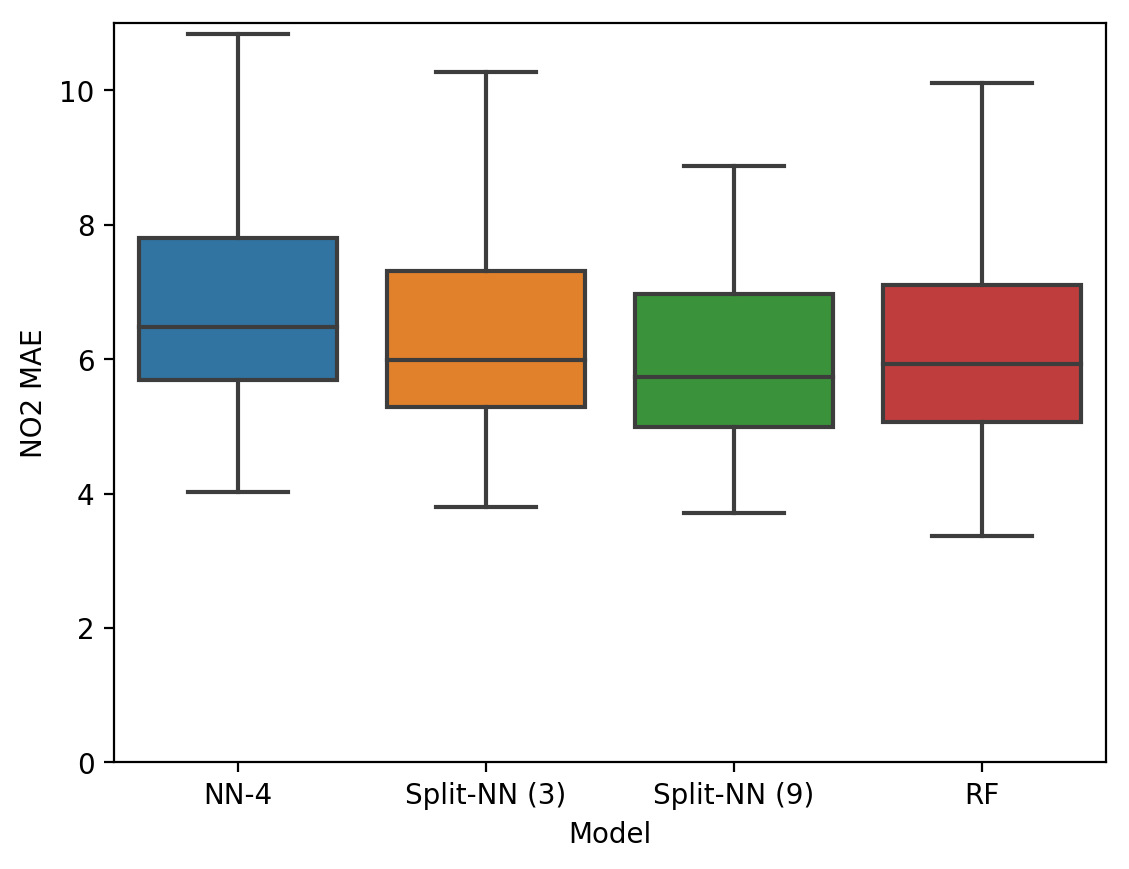
\includegraphics[width=\textwidth]{results/split-no2-location-level1-mae}
\caption{Level 1 NO\textus{2}}
\end{subfigure}
\begin{subfigure}{0.45\textwidth}
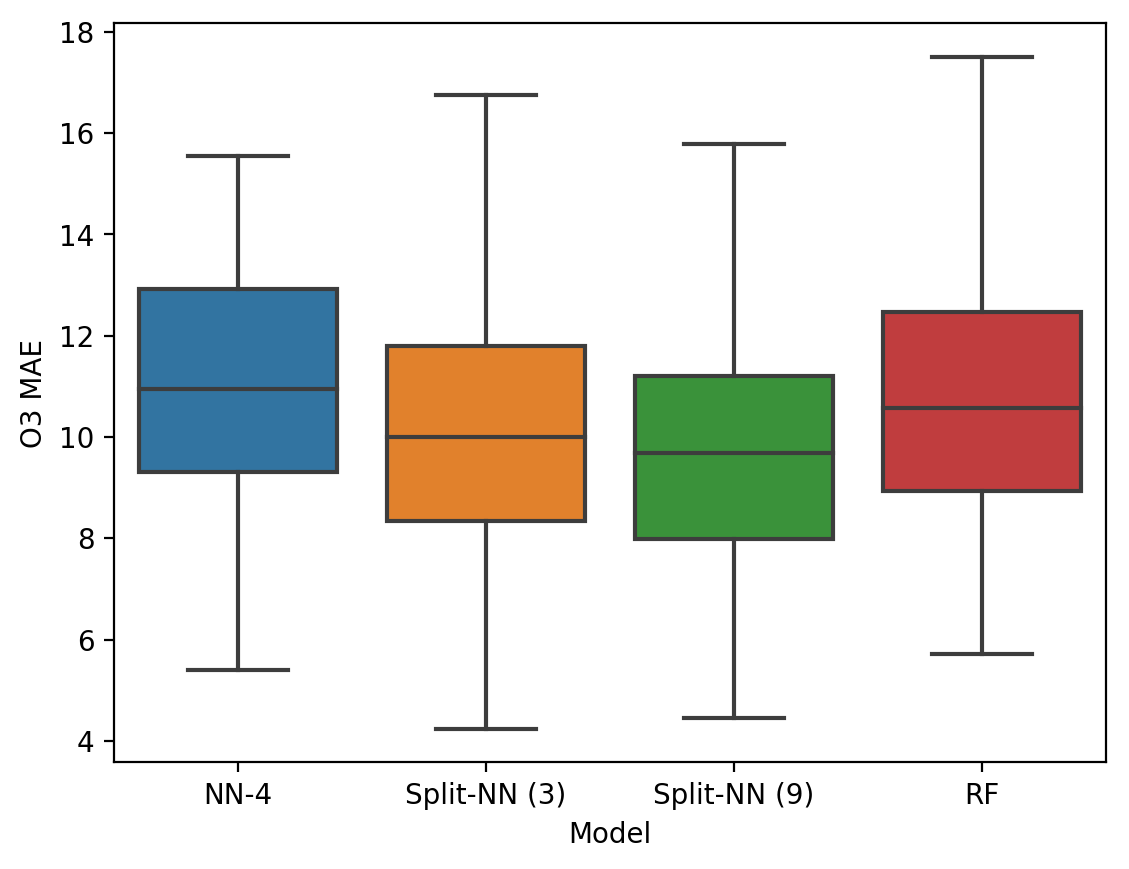
\includegraphics[width=\textwidth]{results/split-o3-location-level1-mae}
\caption{Level 1 O\textus{3}}
\end{subfigure}
\begin{subfigure}{0.45\textwidth}
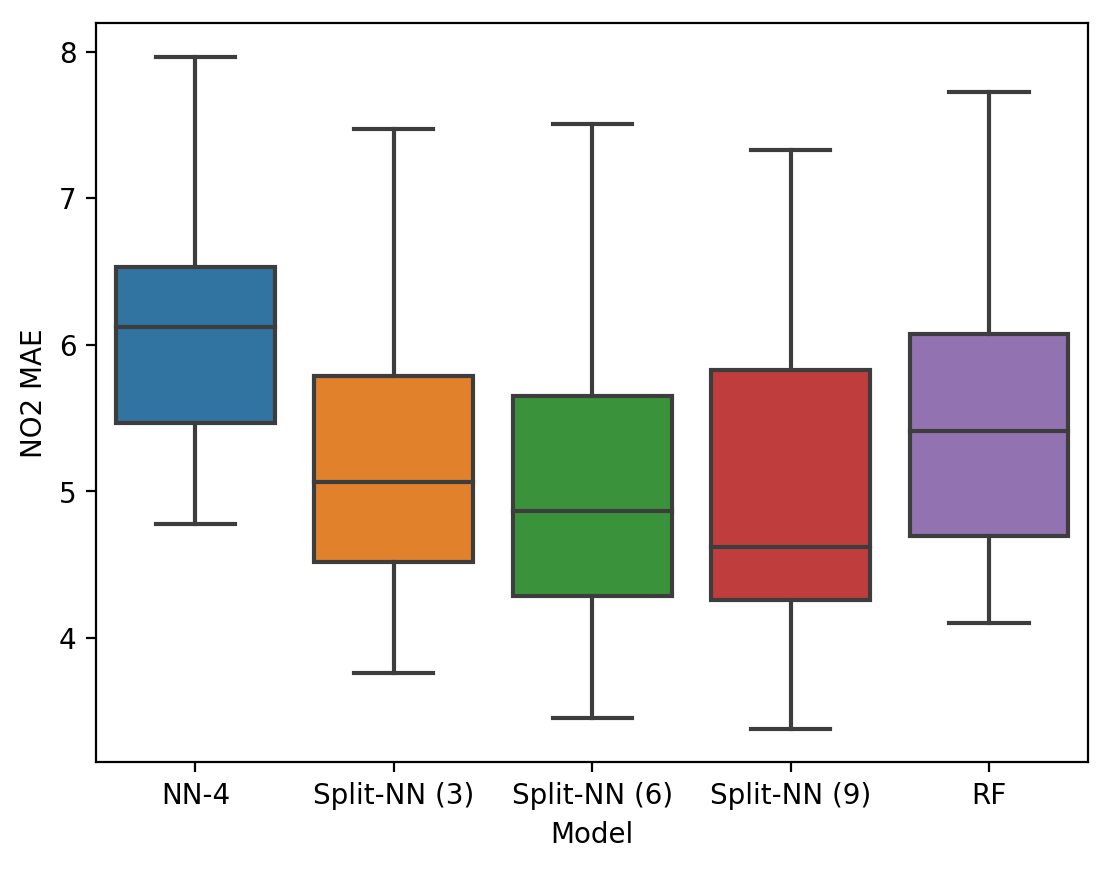
\includegraphics[width=\textwidth]{results/split-no2-location-level2-mae}
\caption{Level 2 NO\textus{2}}
\end{subfigure}
\begin{subfigure}{0.45\textwidth}
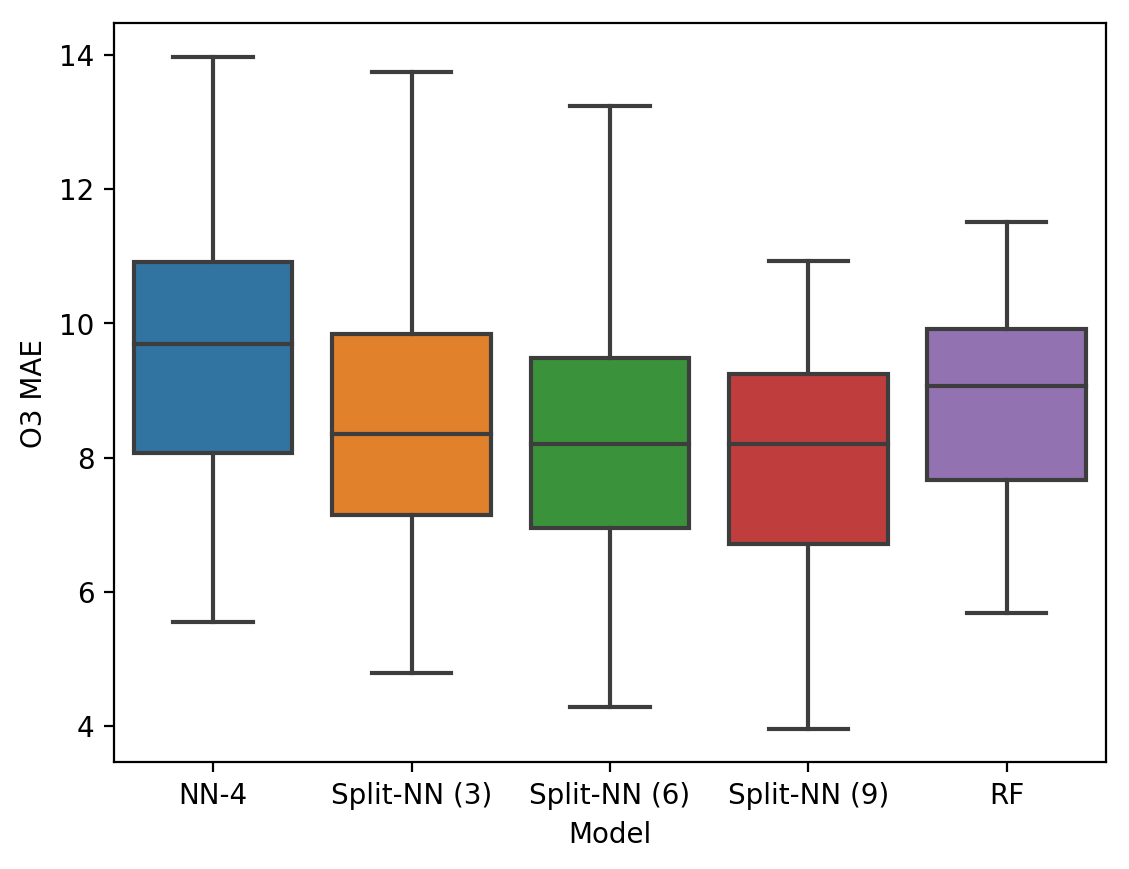
\includegraphics[width=\textwidth]{results/split-o3-location-level2-mae}
\caption{Level 2 O\textus{3}}
\end{subfigure}
\caption{Results of evaluating the split-NN model with a linear regression first stage, compared against the RF model in both Level 1 and Level 2 comparisons. The split-NN model has a lower mean and median error in all conditions. Boxplots are pictured without outliers for clarity.}
\label{fig:split-results-lrfe}
\end{figure}

% Seasonal plots
%\begin{subfigure}{0.45\textwidth}
%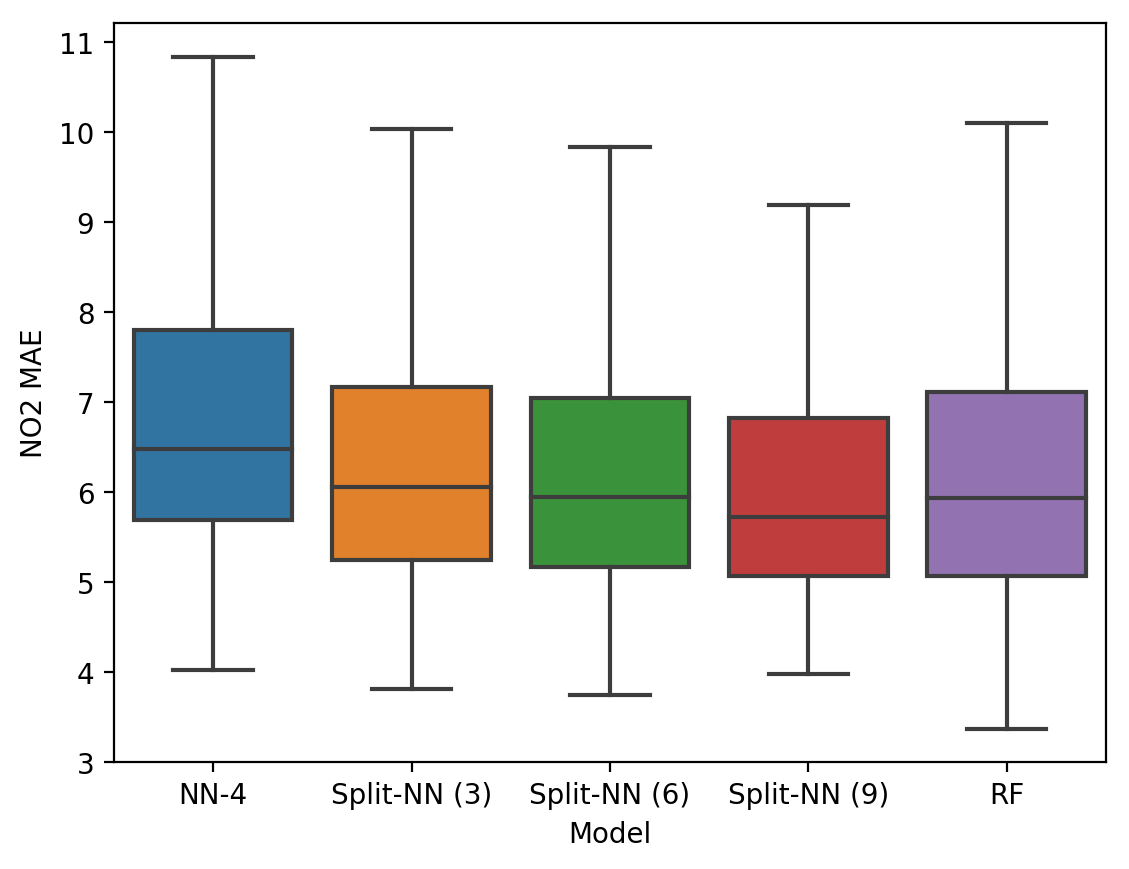
\includegraphics[width=\textwidth]{results/split-no2-seasonal-mae}
%\caption{Level 1 Seasonal Split-NN neural network results (NO\textus{2})}
%\end{subfigure}
%\begin{subfigure}{0.45\textwidth}
%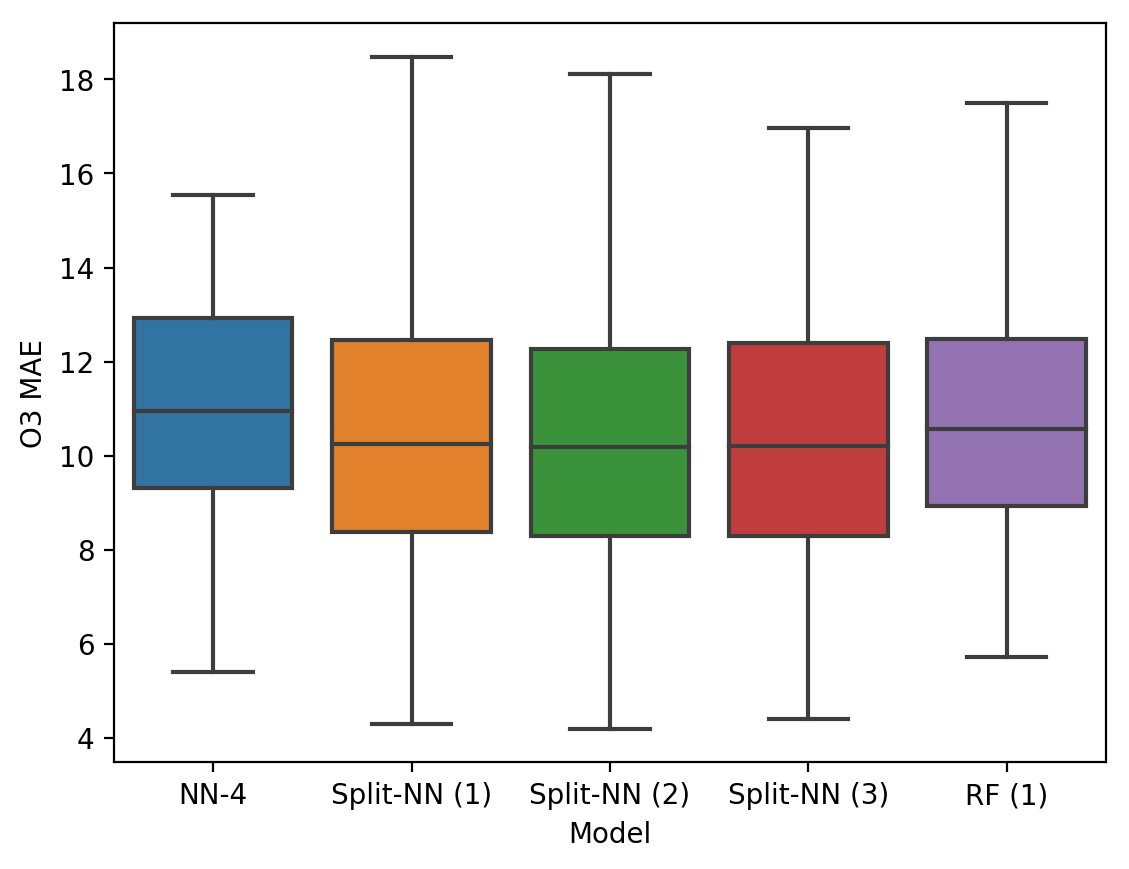
\includegraphics[width=\textwidth]{results/split-o3-seasonal-mae}
%\caption{Level 1 Seasonal Split-NN neural network results (O\textus{3})}
%\end{subfigure}
%\begin{subfigure}{0.45\textwidth}
%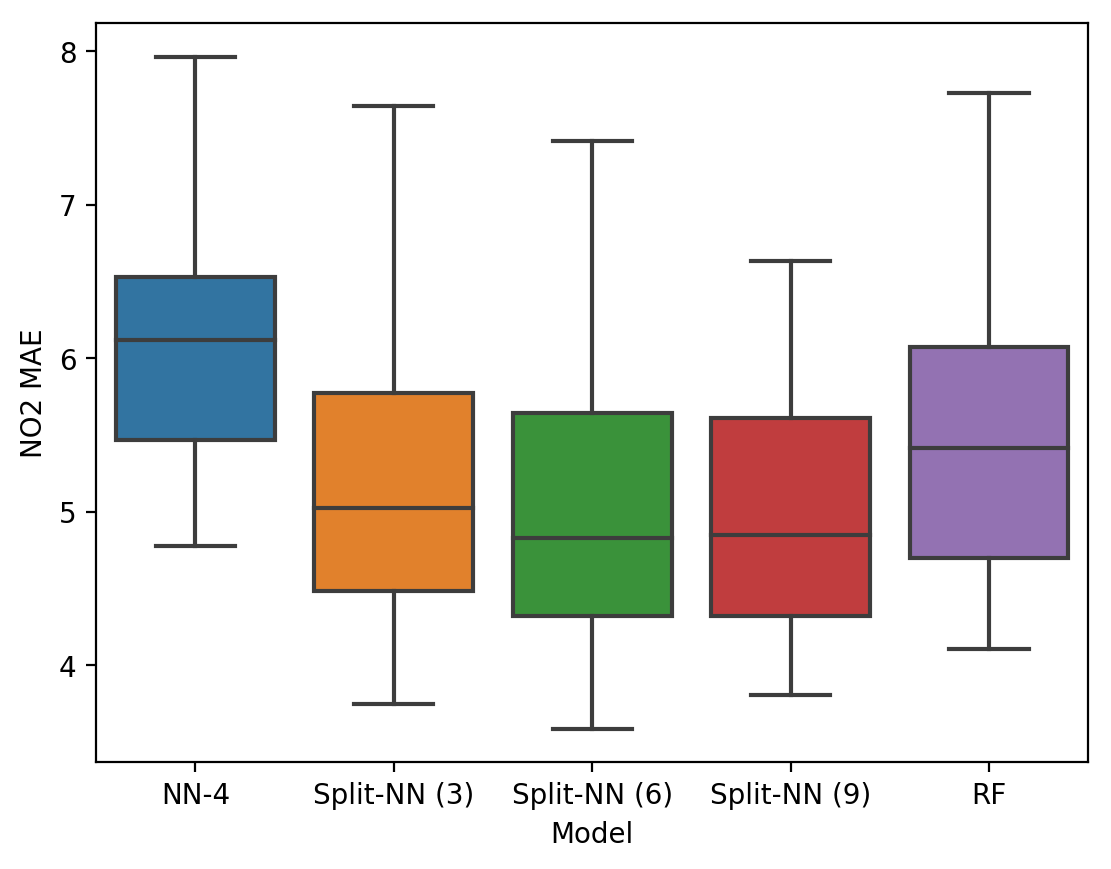
\includegraphics[width=\textwidth]{results/split-no2-seasonal-level2-mae}
%\caption{Level 2 Seasonal Split-NN neural network results (NO\textus{2})}
%\end{subfigure}
%\begin{subfigure}{0.45\textwidth}
%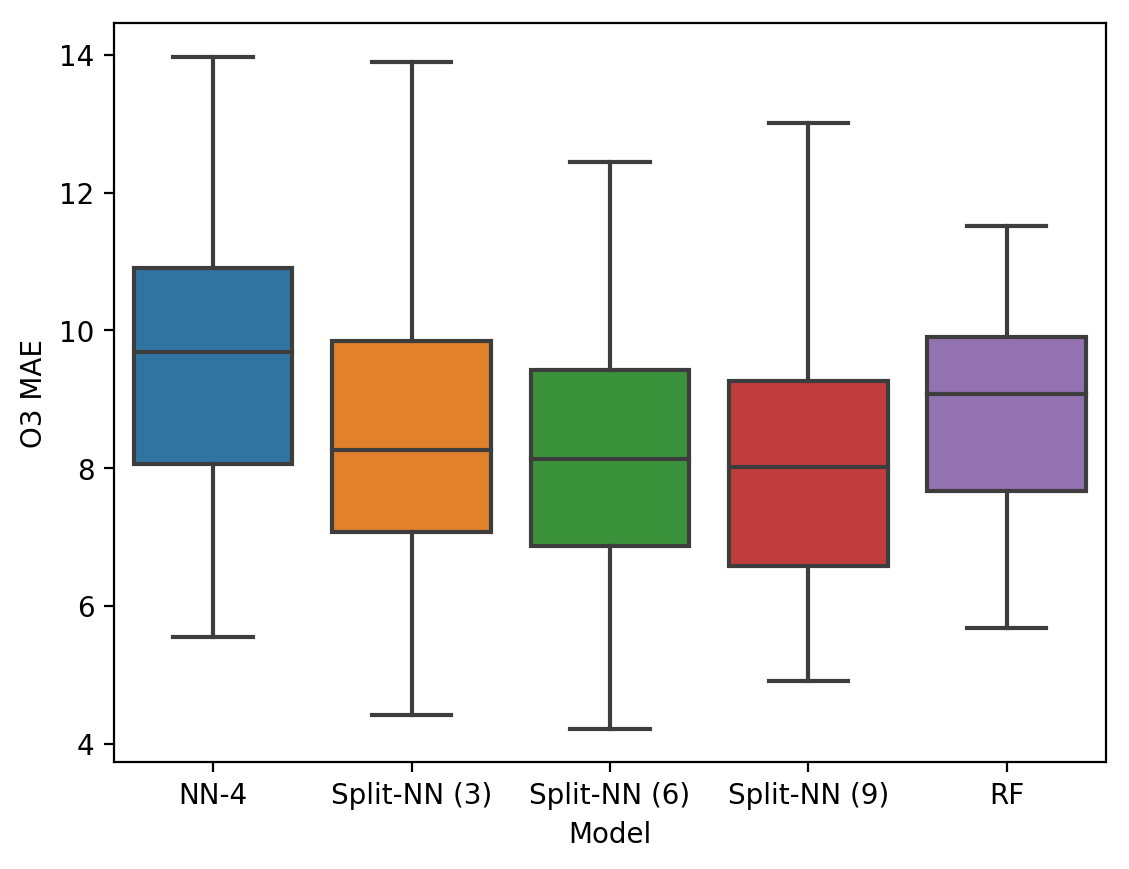
\includegraphics[width=\textwidth]{results/split-o3-seasonal-level2-mae}
%\caption{Level 2 Seasonal Location Split-NN neural network results (O\textus{3})}
%\end{subfigure}
\begin{figure}[H]
\centering
\begin{subfigure}{0.45\textwidth}
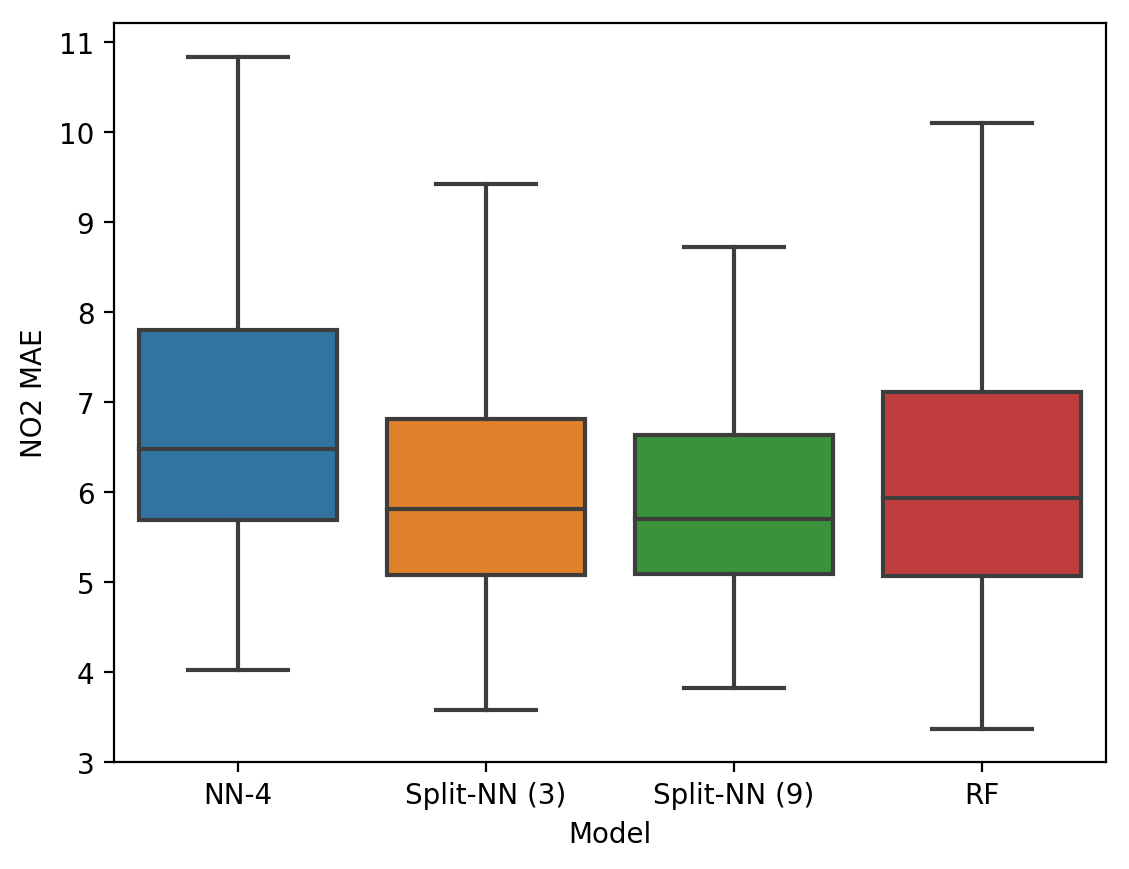
\includegraphics[width=\textwidth]{results/split-no2-location-level1-big-mae}
\caption{Level 1 NO\textus{2}}
\end{subfigure}
\begin{subfigure}{0.45\textwidth}
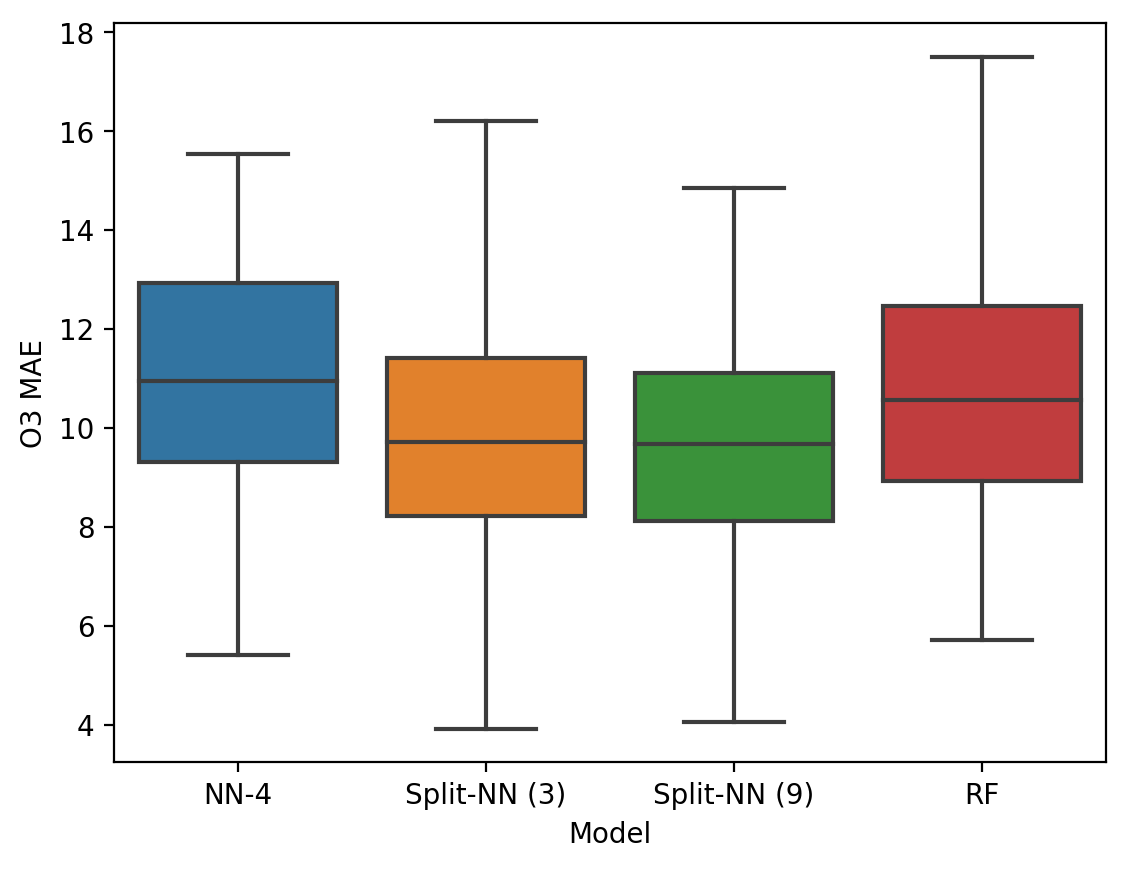
\includegraphics[width=\textwidth]{results/split-o3-location-level1-big-mae}
\caption{Level 1 O\textus{3}}
\end{subfigure}
\begin{subfigure}{0.45\textwidth}
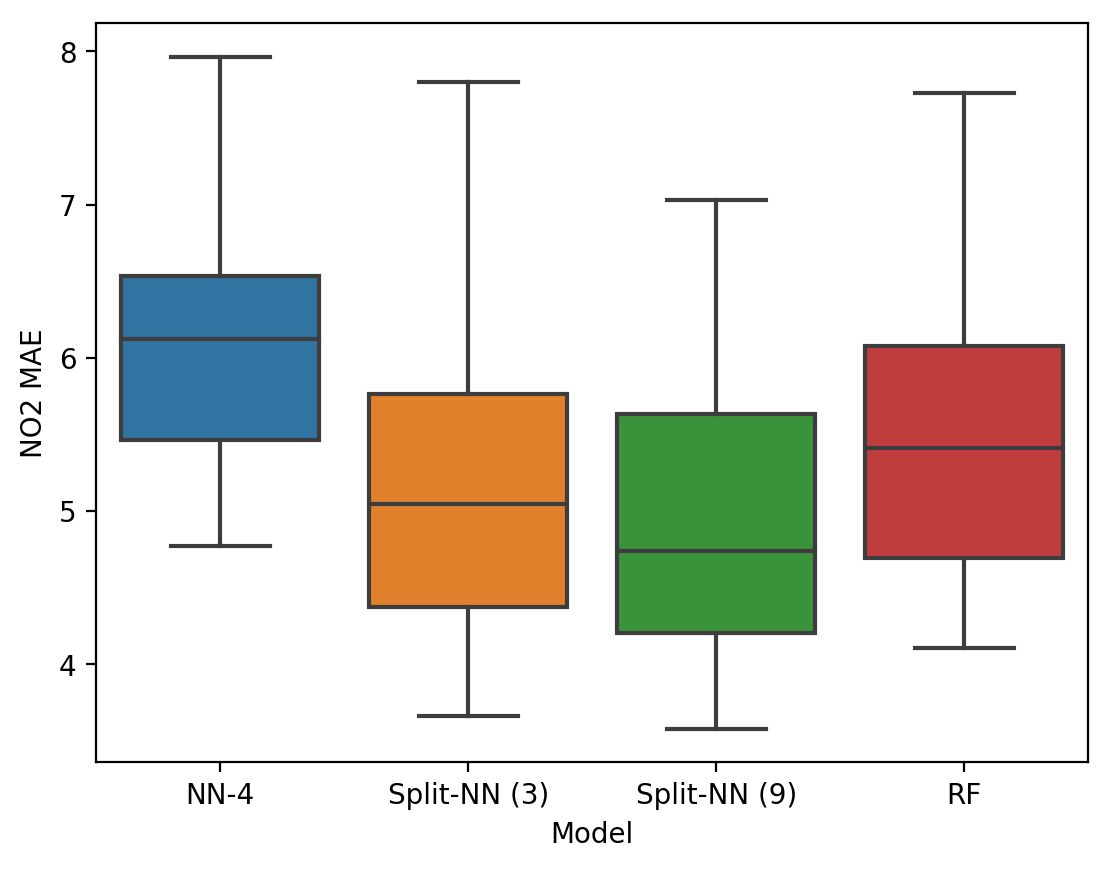
\includegraphics[width=\textwidth]{results/split-no2-location-level2-big-mae}
\caption{Level 2 NO\textus{2}}
\end{subfigure}
\begin{subfigure}{0.45\textwidth}
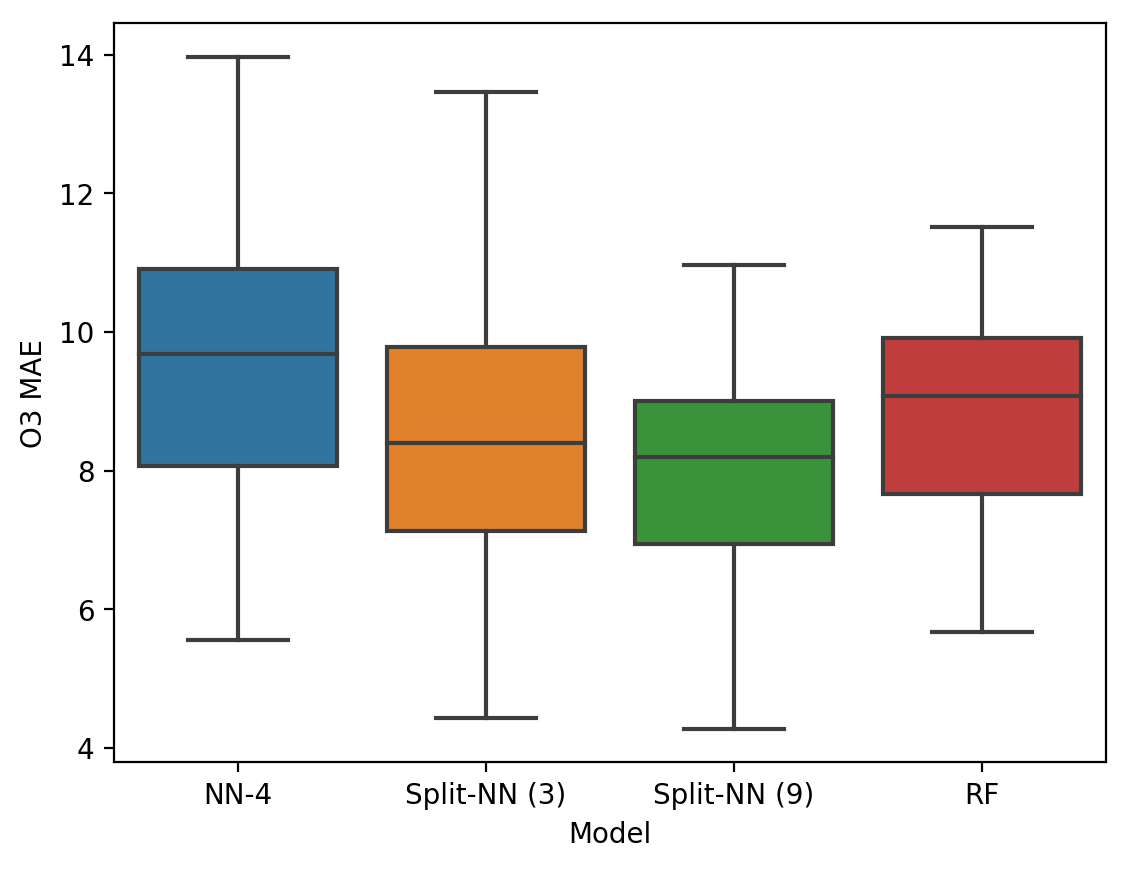
\includegraphics[width=\textwidth]{results/split-o3-location-level2-big-mae}
\caption{Level 2 O\textus{3}}
\end{subfigure}
\caption{Results of evaluating the split-NN model with a linear regression first stage, compared against the RF model in both Level 1 and Level 2 comparisons. The split-NN model has a lower mean and median error in all conditions. Boxplots are pictured without outliers for clarity.}
\label{fig:split-results-nnfe}
\end{figure}

\iffalse
We also evaluated the calibration of a new sensor package using the split-NN approach. As described in Section~\ref{sec:split-nn}, rather than retraining a full calibration model when a new, uncalibrated sensor needs to be deployed, we can colocate it with an already-calibrated low-cost sensor. We then train a new sensor model for the new board, regressing to match the sensor model outputs from the colocated boards. Since the sensor model outputs intermediate values that are then fed into a global calibration model, we have effectively calibrated a new board just through the sensor model. Using this approach we find \todo{WGG: how?} that on average, \todo{WGG: is this additional error over doing it from scratch?  Sounds high.  Our new test will help here.} we incur 3.79 NO\textus{2} MAE and 6.07 O\textus{3} MAE.
\fi


%\begin{figure}
%    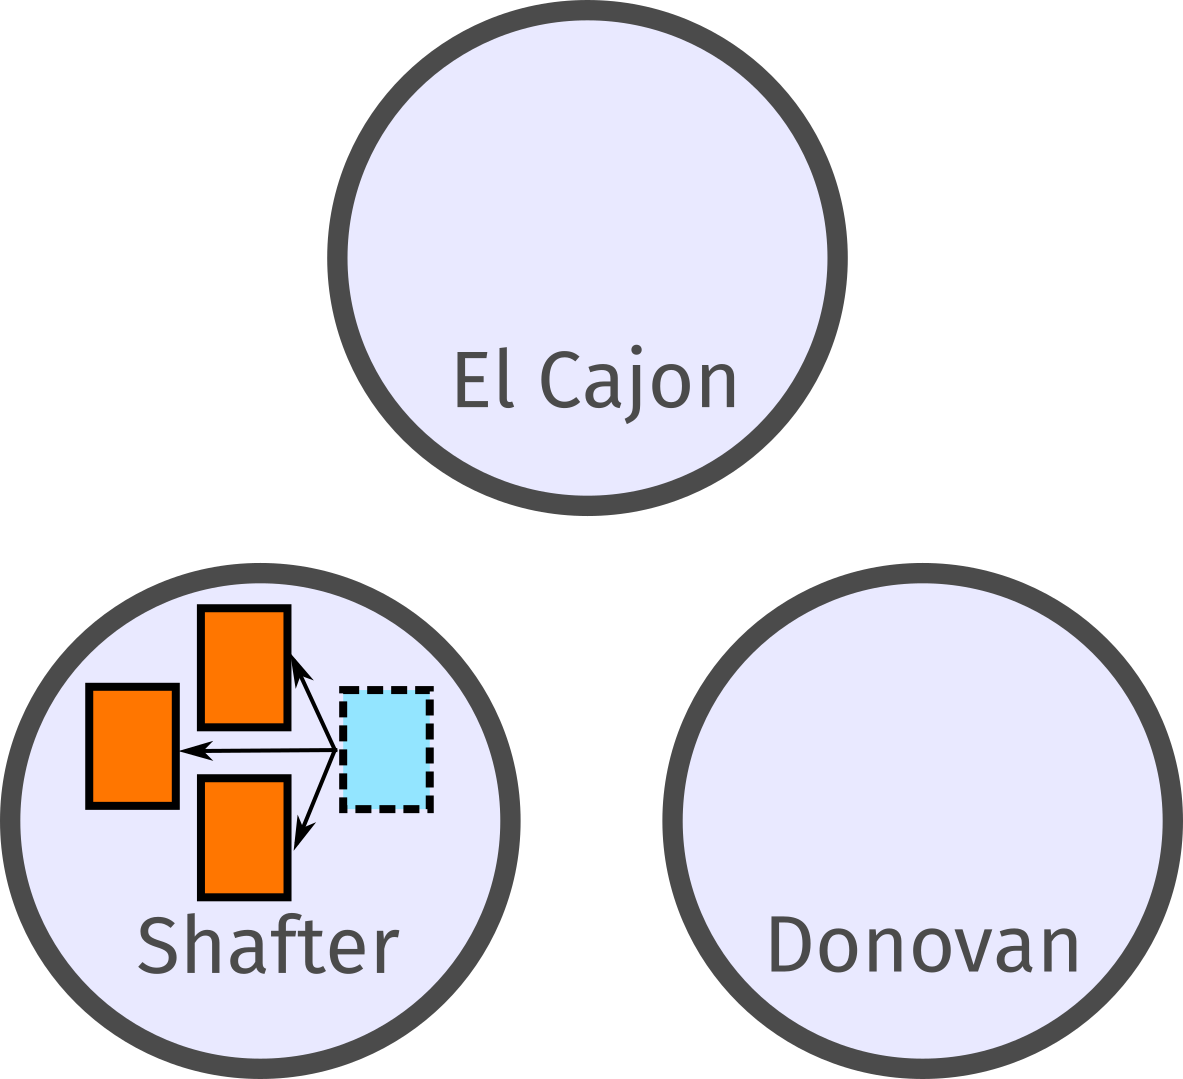
\includegraphics[width=0.3\textwidth]{writeup/img/levels-retrain}
%    \caption{Calibrating a new board $N + 1$}
%\end{figure}

\iffalse

\begin{itemize}
    \item Given these failure modes, how can data collection and model training be improved to overcome these failures?
      \begin{itemize}
          \item Collect data from multiple sites and either:
          \begin{itemize}
            \item Average models over multiple diverse locations 
            \item Pool all the data together and build a single model
          \end{itemize}
      \end{itemize}
    \item Given that it is typical to calibrate many sensors, how should calibration data from multiple sensors be employed to achieve the best results?
      \begin{itemize}
          \item Collect data from all sensors to be calibrated and build a single shared model
      \end{itemize}
    \item Finally, (how) can multiple-site techniques and multiple-sensor techniques be combined?
      \begin{itemize}
         \item Neural networks work, and random forest doesn’t, because they are more modular (differentiability)
      \end{itemize}
    \item Can a new sensor can be affordably and accurately calibrated without having to repeat the whole data collection cycle?
      \begin{itemize}
          \item Simple colocation with a single sensor
          \item Match new sensor to the global model through colocation with one of the calibrated sensors
      \end{itemize}
\end{itemize}
\fi

\subsection{Discussion}

As low-cost sensor studies move from understanding sensor signal performance to how this performance is affected by moving sensors to new sampling locations or utilizing them in new applications, it is important that the results are translated into best practices to support the collection of usable high quality data. This is particularly important given the interest in sensors by community-based organizations and citizen scientists. Although the present study examined only electrochemical O\textus{3} and NO\textus{2} sensors and the sampling sites were limited to three in California, it adds to a body of evidence that location matters in the calibration of low-cost sensors because the background environmental conditions matter.  With this in mind, we make the following observations and recommendations.

%Given that the present study examined only electrochemical O\textus{3} and NO\textus{2} sensors and the sampling sites were limited to three in California, there is a need to continue examining different sensors and to learn more about the consistency of results across locations and situations. 
We observed how prediction performance degrades when a sensor is moved to a new location, especially for high-capacity modeling techniques. In particular, training a complex random forest calibration model will likely result in very low error at a colocated site but can incur significant error at a different site. Although their predictions at a new site will have lower error than linear regression, the error they have at the training site will likely not be representative of their error in practice.  A linear model, on the other hand, despite not predicting as well at the training site, will not have significantly more error at testing time.  Thus, if it is important to know the likely error of your calibration model under transfer, it would be best to use a low-capacity method like linear regression.

When we drilled down to investigate the contributors to error when changing location, we found that bias error was a significant contributor in many cases. This is interesting because bias error indicates a loss of accuracy (a non-random additive error) rather than a loss of precision (random noise). This suggests that when moving a sensor to a new location, if the bias can somehow be detected, then it may be possible to make a bias correction to improve model performance. This result also motivates the use of the split neural network architecture, which has a model-specific correction stage that is designed to learn unbiased representations of sensor measurements.

We had expected that training at multiple sites would provide much better transferability, but the improvements were not substantial, suggesting that the high-capacity models were mostly improving due to implicit overlap in distributions and not actual generalization.  This suggests that calibration should be directed at capturing the widest conditions possible, for example using many field sites with varying conditions, so as to create an overlap between the distributions of training and use.  This recommendation is further supported by the observation that the Level 3 benchmarks performed nearly as well as the Level 0 benchmarks, in spite of carrying the load of a much wider distribution in the models.

The split-NN approach provides a potentially economical approach to creating overlap in distributions since sensors can share their data for calibration.  That is, when calibrating multiple sensors, rather than colocating multiple sensors at a field site and rotating those sensors over time, it makes sense to distribute the sensors to as many field sites as possible to capture the widest distribution of conditions.  More study will be required to see how well the split-NN approach scales.

\todo{WGG: graphs don't show this: Location Test will help.} Only when we employed the split-NN technique did we get the expected results.  
\todo{WGG: something about training a new sensor?}

%Considering these limitations, there are a number of recommendations drawn from the results of this study that may be useful for communities and citizens scientists interested in using low-cost sensors. 
% 
%\begin{itemize}
%    \item When conducting a “field calibration” (or colocating your sensors with trusted reference monitors), colocating your sensors at multiple reference locations will likely improve the reliability of the data from your sensors when they are moved to the field sites.
%    \item If you are conducting a field calibration and are unsure of how different your field sites are from your calibration site, consider choosing a simpler calibration model, such as a multiple linear regression model.
%    \item When conducting a field calibration, placing sensors at different colocation sites then pooling that data and building a calibration model built on data from multiple sites will result in a calibration model that is more robust in new locations. 
%end{itemize}

%Essentially, the recommendations presented here emphasize the need for thoughtful study design when using low-cost sensors. Users need to be thoughtful about where and how calibration is occurring, as well as any potential repercussions of a particular choice – for example the decision to use a high-capacity machine learning model.


%Previous text:
%
%\begin{itemize}
%    \item \todo{Model size}
%    \item \todo{Calibrate over a lot of sites}
%    \item If one doesn't have access to multiple sites (or only two instead of three), can multiple locations be approximated by just training longer at one site? \emph{maybe}
%    \item Translate what we've learned into practical advice for an average citizen scientist group - how can they use this information to improve their work and given typical real-world constraints where can they focus their efforts in order to get the best data quality possible (maybe this section should include a list of hypothetical) 
%\end{itemize}

\section{Conclusion}

As low-cost gas-phase sensors are increasingly being adopted for citizen science efforts and community-based studies, there is a need to better understand what contributes to accurate sensing.  A key question is how a change in background environmental or pollutant conditions, often unique to a location, affects accuracy.  A rotating deployment strategy enabled benchmarking the transferability of models and investigating how to improve accuracy. We found that overfitting is a concern, especially when transferring high-capacity models like random forest that are trained with data that will not be representative of the conditions of use. Our benchmarks indicate that widening the data distribution is a good strategy to make models more robust to transfer, but that the best results require the training distribution to contain the distribution encountered in use.  A tantalizing result is that much of the error introduced by transfer was bias, which may be correctable.  When multiple sensors based on the same technology are being trained at the same time, we found that a split neural network architecture increases the robustness of model transfer by giving a sensor's model access to normalized data from other sensors, even at other locations, hence widening the distribution without requiring additional data collection.  This method also enables accurately calibrating new sensors against existing calibrated sensors at incremental cost.

In the future work we will be extending this work to answer open questions that we believe are relevant to the future of low-cost sensor calibration.  As one example, there are questions about the effect of temporal resolution on accuracy. Currently, our MetaSense sensors are sampled every five seconds, but the ground-truth data provided from reference monitors is minute-averaged. By averaging our own sensor measurements every minute, we discard data that could be relevant for calibration. Recent advances in recurrent neural networks for sequence prediction might help leverage the high-resolution data for robust prediction. As a second example, a potential application of low-cost sensing is truly mobile sensing with person- or vehicle-mounted sensors. Deployments such as these will raise questions about the effects of mobility on sensing accuracy, such as rapidly changing conditions, with few studies to date~\citep{arfire2016mitigating}.

% A dynamic data distribution is a challenge that we hope our methods can generalize to.

\section{Acknowledgements}

We would like to thank partners at the San Diego Air Pollution Control District as well as San Joaquin Valley Air Pollution Control District for their support throughout this deployment. 

\iffalse
\begin{itemize}
    \item What is the tradeoff between resolution and accuracy, if any. 
    \item Mobility causes fast changes. Brief high exposures could be harmful.
    \item Our sensors change slowly, taking up to 30 seconds to respond to a change in signal
    \item Noise, Drift?
\end{itemize}
\fi

\bibliographystyle{copernicus}
\bibliography{main.bib}


%%%%%%%%%%%%%%%%%%%%%%%%%%%%%%%%%%%%%%%%%%%%%
%%%%%%%%%%%%%%%%%%%%%%%%%%%%%%%%%%%%%%%%%%%%%
\clearpage
\appendix
\setcounter{table}{0}

\iffalse
\section{Data}

We have been collecting data from nine boards
from three sites in southern California.
\begin{enumerate}
    \item El Cajon
    \item Donovan
    \item Shafter
\end{enumerate}
We have split up the boards and rotated the boards
between locations every two weeks (see \autoref{tab:board-rotations}).

We do not have CO data for Shafter and Donovan, so we will focus only on
O\textus{3} and NO\textus{2}.
\fi


\section{Environment and Pollutant Distributions}\label{Distributions}

%\todo{Have these been updated to reflect the data we are using? (i.e., from R2, R2, and R4}
%\todo{Recommend for the Distribution section just keep plots B5, B6, B8, B10 - those would be sufficient, keeping all might be too much (WGG: DONE)}


%\subsection{Environment}

\iffalse

\begin{figure}[H]
\centering
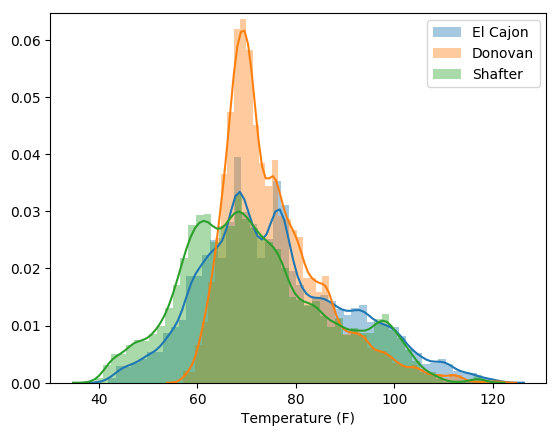
\includegraphics[width=0.5\textwidth]{results/distributions/temperature.png}
\caption{Temperature distribution based on
location}
\label{fig:temperature}
\end{figure}

\begin{figure}[H]
\centering
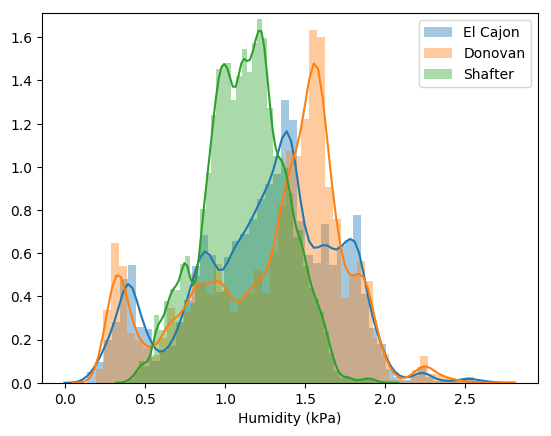
\includegraphics[width=0.5\textwidth]{results/distributions/humidity.png}
\caption{Absolute humidity distribution based on
location}
\label{fig:humidity}
\end{figure}

\begin{figure}[H]
\centering
\begin{subfigure}{0.32\textwidth}
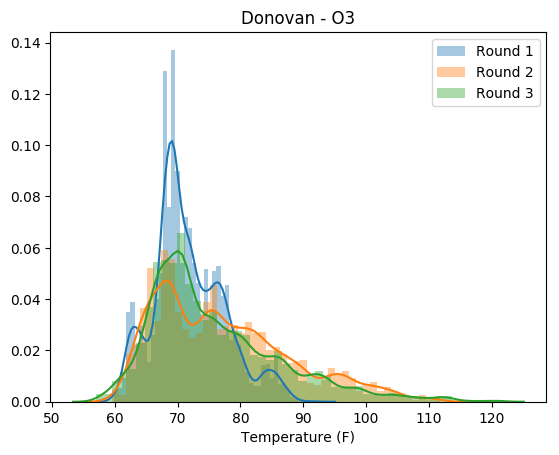
\includegraphics[width=\textwidth]{results/distributions/location_donovan_temperature.png}
\caption{Donovan}
\end{subfigure}
\begin{subfigure}{0.32\textwidth}
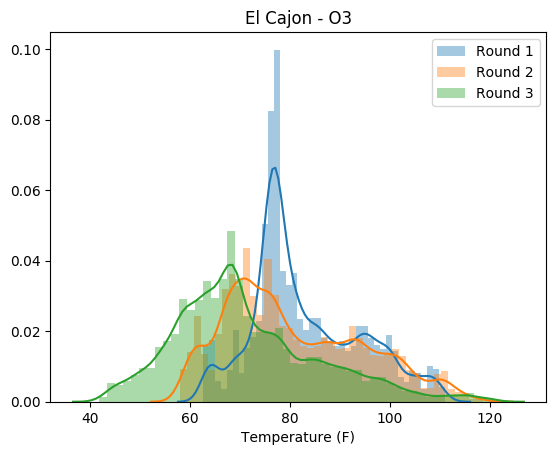
\includegraphics[width=\textwidth]{results/distributions/location_elcajon_temperature.png}
\caption{El Cajon}
\end{subfigure}
\begin{subfigure}{0.32\textwidth}
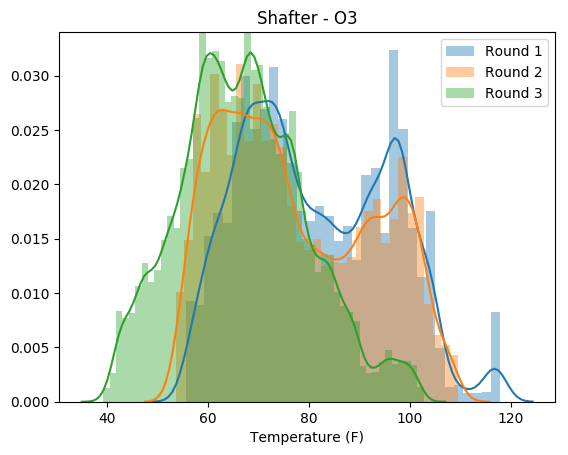
\includegraphics[width=\textwidth]{results/distributions/location_shafter_temperature.png}
\caption{Shafter}
\end{subfigure}
\caption{Temperature at locations}
\label{fig:temperature-locations}
\end{figure}

\begin{figure}[H]
\centering
\begin{subfigure}{0.32\textwidth}
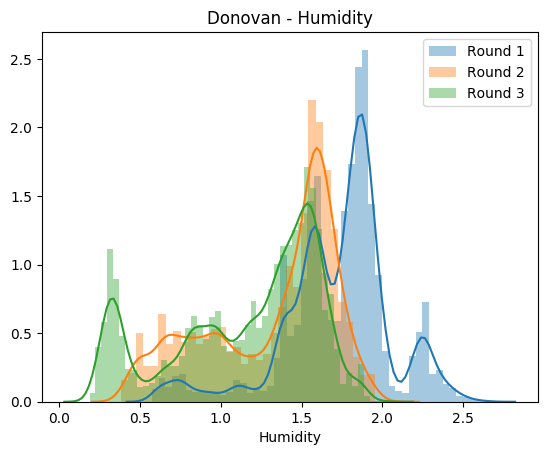
\includegraphics[width=\textwidth]{results/distributions/location_donovan_humidity.png}
\caption{Donovan}
\end{subfigure}
\begin{subfigure}{0.32\textwidth}
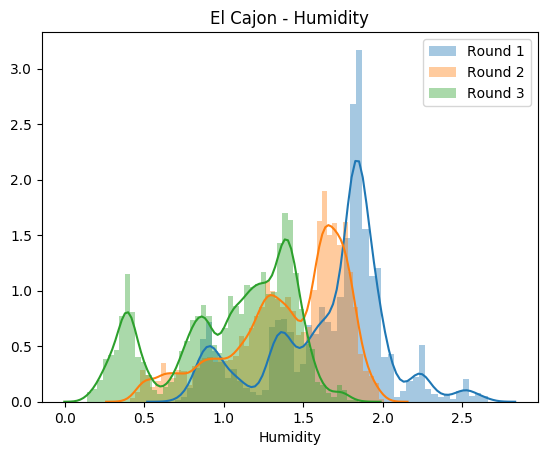
\includegraphics[width=\textwidth]{results/distributions/location_elcajon_humidity.png}
\caption{El Cajon}
\end{subfigure}
\begin{subfigure}{0.32\textwidth}
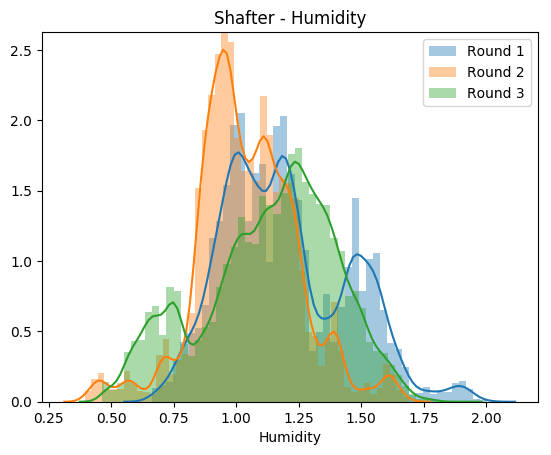
\includegraphics[width=\textwidth]{results/distributions/location_shafter_humidity.png}
\caption{Shafter}
\end{subfigure}
\caption{Absolute humidity at locations}
\label{fig:humidity-locations}
\end{figure}

\fi

\begin{figure}[H]
\centering
\begin{subfigure}{0.32\textwidth}
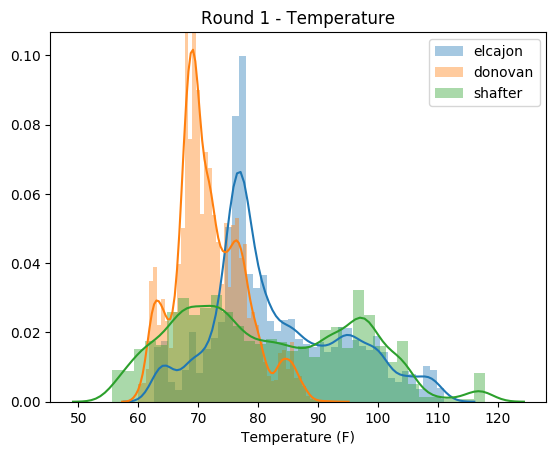
\includegraphics[width=\textwidth]{results/distributions/round1_temperature.png}
\caption{Round 1}
\end{subfigure}
\begin{subfigure}{0.32\textwidth}
.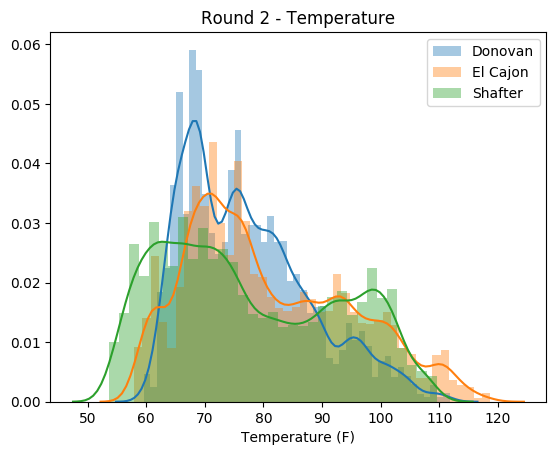
\includegraphics[width=\textwidth]{results/distributions/round2_temperature.png}
\caption{Round 2}
\end{subfigure}
\begin{subfigure}{0.32\textwidth}
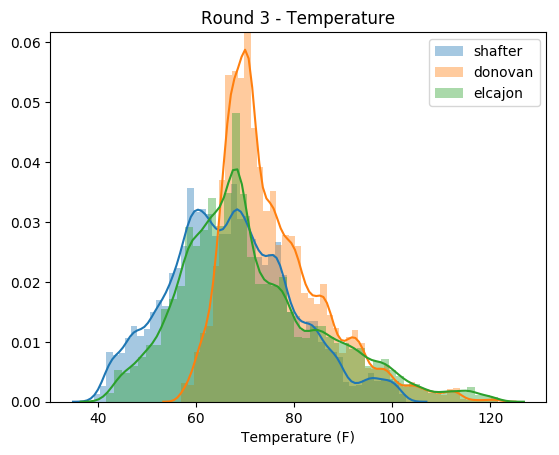
\includegraphics[width=\textwidth]{results/distributions/round3_temperature.png}
\caption{Round 3}
\end{subfigure}
\caption{Temperature distributions for each location, by round.}
\label{fig:temperature-rounds}
\end{figure}

\begin{figure}[H]
\centering
\begin{subfigure}{0.32\textwidth}
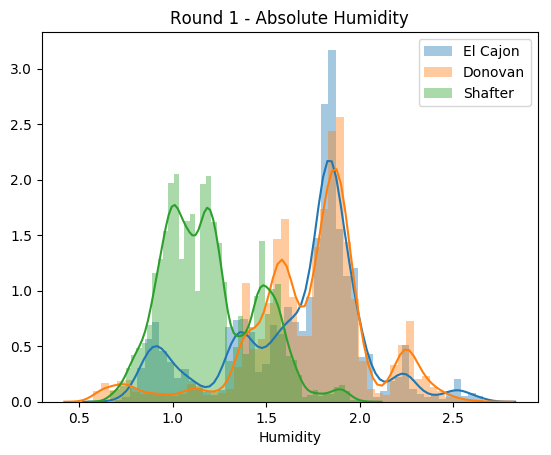
\includegraphics[width=\textwidth]{results/distributions/round1_humidity.png}
\caption{Round 1}
\end{subfigure}
\begin{subfigure}{0.32\textwidth}
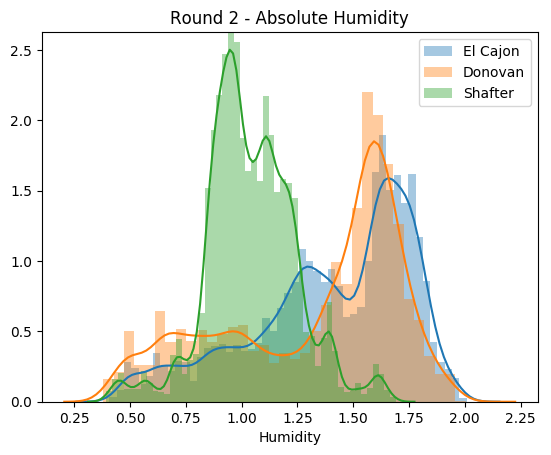
\includegraphics[width=\textwidth]{results/distributions/round2_humidity.png}
\caption{Round 2}
\end{subfigure}
\begin{subfigure}{0.32\textwidth}
\includegraphics[width=\textwidth]{results/distributions/round3_humidity.png}
\caption{Round 3}
\end{subfigure}
\caption{Humidity distributions for each location, by round.}
\label{fig:humidity-rounds}
\end{figure}


%\subsection{Pollutant values}

\iffalse

\begin{figure}[H]
\centering
\begin{subfigure}{0.32\textwidth}
\includegraphics[width=\textwidth]{results/distributions/location_donovan_no2.png}
\caption{Donovan}
\end{subfigure}
\begin{subfigure}{0.32\textwidth}
\includegraphics[width=\textwidth]{results/distributions/location_elcajon_no2.png}
\caption{El Cajon}
\end{subfigure}
\begin{subfigure}{0.32\textwidth}
\includegraphics[width=\textwidth]{results/distributions/location_shafter_no2.png}
\caption{Shafter}
\end{subfigure}
\caption{NO\textus{2} at locations}
\label{fig:no2-locations}
\end{figure}

\fi

\begin{figure}[H]
\centering
\begin{subfigure}{0.32\textwidth}
\includegraphics[width=\textwidth]{results/distributions/round1_no2.png}
\caption{Round 1}
\end{subfigure}
\begin{subfigure}{0.32\textwidth}
\includegraphics[width=\textwidth]{results/distributions/round2_no2.png}
\caption{Round 2}
\end{subfigure}
\begin{subfigure}{0.32\textwidth}
\includegraphics[width=\textwidth]{results/distributions/round3_no2.png}
\caption{Round 3}
\end{subfigure}
\caption{NO\textus{2} distributions for each location, by round.}
\label{fig:no2-rounds}
\end{figure}

\iffalse

\begin{figure}[H]
\centering
\begin{subfigure}{0.32\textwidth}
\includegraphics[width=\textwidth]{results/distributions/location_donovan_o3.png}
\caption{Round 1}
\end{subfigure}
\begin{subfigure}{0.32\textwidth}
\includegraphics[width=\textwidth]{results/distributions/location_elcajon_o3.png}
\caption{Round 2}
\end{subfigure}
\begin{subfigure}{0.32\textwidth}
\includegraphics[width=\textwidth]{results/distributions/location_shafter_o3.png}
\caption{Round 3}
\end{subfigure}
\caption{O\textus{3} at locations}
\label{fig:o3-locations}
\end{figure}

\fi

\begin{figure}[H]
\centering
\begin{subfigure}{0.32\textwidth}
\includegraphics[width=\textwidth]{results/distributions/round1_o3.png}
\caption{Round 1}
\end{subfigure}
\begin{subfigure}{0.32\textwidth}
\includegraphics[width=\textwidth]{results/distributions/round2_o3.png}
\caption{Round 2}
\end{subfigure}
\begin{subfigure}{0.32\textwidth}
\includegraphics[width=\textwidth]{results/distributions/round3_o3.png}
\caption{Round 3}
\end{subfigure}
\caption{O\textus{3} distributions for each location, by round.}
\label{fig:o3-rounds}
\end{figure}

\section{Additional Error Density Plots}\label{sec:remaining-error-density-plots}

\begin{figure}[H]
\centering
\begin{subfigure}{0.33\textwidth}
\includegraphics[width=\textwidth]{\baselinedir/linear/error_density_temperature_donovan_O3.png}
\caption{LR, trained at Donovan}
\end{subfigure}
\begin{subfigure}{0.33\textwidth}
\includegraphics[width=\textwidth]{\baselinedir/linear/error_density_temperature_elcajon_O3.png}
\caption{LR, trained at El Cajon}
\end{subfigure}
\begin{subfigure}{0.33\textwidth}
\includegraphics[width=\textwidth]{\baselinedir/linear/error_density_temperature_shafter_O3.png}
\caption{LR, trained at Shafter}
\end{subfigure}
\begin{subfigure}{0.33\textwidth}
\includegraphics[width=\textwidth]{\baselinedir/subu/error_density_temperature_donovan_O3.png}
\caption{RF, trained at Donovan}
\end{subfigure}
\begin{subfigure}{0.33\textwidth}
\includegraphics[width=\textwidth]{\baselinedir/subu/error_density_temperature_elcajon_O3.png}
\caption{RF, trained at El Cajon}
\end{subfigure}
\begin{subfigure}{0.33\textwidth}
\includegraphics[width=\textwidth]{\baselinedir/subu/error_density_temperature_shafter_O3.png}
\caption{RF, trained at Shafter}
\end{subfigure}
\caption{Error density plots for O\textus{3} versus temperature for both Linear Regression (LR) and Random Forest (RF) in a Level 1 benchmark.}
\label{fig:error-density-O3-temp}
\end{figure}


\begin{figure}[H]
\centering
\begin{subfigure}{0.33\textwidth}
\includegraphics[width=\textwidth]{\baselinedir/linear/error_density_absolute-humidity_donovan_NO2.png}
\caption{LR, trained at Donovan}
\end{subfigure}
\begin{subfigure}{0.33\textwidth}
\includegraphics[width=\textwidth]{\baselinedir/linear/error_density_absolute-humidity_elcajon_NO2.png}
\caption{LR, trained at El Cajon}
\end{subfigure}
\begin{subfigure}{0.33\textwidth}
\includegraphics[width=\textwidth]{\baselinedir/linear/error_density_absolute-humidity_shafter_NO2.png}
\caption{LR, trained at Shafter}
\end{subfigure}
\begin{subfigure}{0.33\textwidth}
\includegraphics[width=\textwidth]{\baselinedir/subu/error_density_absolute-humidity_donovan_NO2.png}
\caption{RF, trained at Donovan}
\end{subfigure}
\begin{subfigure}{0.33\textwidth}
\includegraphics[width=\textwidth]{\baselinedir/subu/error_density_absolute-humidity_elcajon_NO2.png}
\caption{RF, trained at El Cajon}
\end{subfigure}
\begin{subfigure}{0.33\textwidth}
\includegraphics[width=\textwidth]{\baselinedir/subu/error_density_absolute-humidity_shafter_NO2.png}
\caption{RF, trained at Shafter}
\end{subfigure}
\caption{Error density plots for NO\textus{2} versus absolute humidity for both Linear Regression (LR) and Random Forest (RF) in a Level 1 benchmark.}
\label{fig:error-density-NO2-humidity}
\end{figure}

\begin{figure}[H]
\centering
\begin{subfigure}{0.33\textwidth}
\includegraphics[width=\textwidth]{\baselinedir/linear/error_density_absolute-humidity_donovan_NO2.png}
\caption{LR, trained at Donovan}
\end{subfigure}
\begin{subfigure}{0.33\textwidth}
\includegraphics[width=\textwidth]{\baselinedir/linear/error_density_absolute-humidity_elcajon_NO2.png}
\caption{LR, trained at El Cajon}
\end{subfigure}
\begin{subfigure}{0.33\textwidth}
\includegraphics[width=\textwidth]{\baselinedir/linear/error_density_absolute-humidity_shafter_NO2.png}
\caption{LR, trained at Shafter}
\end{subfigure}
\begin{subfigure}{0.33\textwidth}
\includegraphics[width=\textwidth]{\baselinedir/subu/error_density_absolute-humidity_donovan_NO2.png}
\caption{RF, trained at Donovan}
\end{subfigure}
\begin{subfigure}{0.33\textwidth}
\includegraphics[width=\textwidth]{\baselinedir/subu/error_density_absolute-humidity_elcajon_NO2.png}
\caption{RF, trained at El Cajon}
\end{subfigure}
\begin{subfigure}{0.33\textwidth}
\includegraphics[width=\textwidth]{\baselinedir/subu/error_density_absolute-humidity_shafter_NO2.png}
\caption{RF, trained at Shafter}
\end{subfigure}
\caption{Error density plots for NO\textus{2} versus absolute-humidity for both Linear Regression (LR) and Random Forest (RF) in a Level 1 benchmark.}
\label{fig:error-density-NO2-temp}
\end{figure}

\iffalse
\section{Basic calibration results}

A calibration model takes in sensor readings and environment
variables and outputs pollutant levels. In this basic setup,
we train a model for each board.
We aim to train models that are robust after moving location.

\begin{table}[H]
\centering
\begin{tabular}{|l|l|}
\hline
\textbf{Level 0} & Train on location A and test on location A \\ \hline
\textbf{Level 1} & Train on location A and test on location B \\ \hline
\textbf{Level 2} & Train on location A and B and test on location C \\ \hline
\textbf{Level 3} & Train on location A, B, and C and test on location A \\ \hline
\end{tabular}
\caption{Description of different types of benchmarks.}
\label{tab:levels}
\end{table}

We benchmark four different models: linear regression (linear), random forest regressors based on \citep{Zimmerman2018},
a 2-layer neural network (NN[2]), and a 4-layer neural network (NN[4]). The ideal model will
both predict pollutant levels accurately and
generalize across locations.

To benchmark, we first take our data sets (25 total, see \autoref{tab:board-rotations}), and partition each into training and testing sets (20\% reserved for testing).
We perform several types of benchmarks,
each to learn about the transferrability of each model (see \autoref{tab:levels}).
In general, we expect Level 0 and Level 3 performance to be the best, as they involve training and testing on data from the same distribution. Furthermore, we expected Level 2 to have lower error than Level 1, because Level 2 is trained on more data and a wider distribution of data (two locations vs one location).
If a model's Level 1 and Level 2 error are close to Level 0 and Level 3, then the model transfers well. Otherwise, the model overfits to its location.


These raw results are in \autoref{sec:simpleresults}. 
We split results into training vs. testing
results, where we expect train performance
to be better than test.
Overall, we see that random forests have the lowest Level 0 and Level 3 error. This is consistent with results we see in \citet{Zimmerman2018}. 
We observe when comparing Level 1 error difference (Level 1 train minus Level 1 test), random forests suffer great
drops in performance.
This hints that RFs are overfitting to the training data, even if they
report the lowest test error for Level 0 and Level 3.  See \autoref{fig:generalization} for 
details.

\begin{figure}[H]
\centering
\begin{subfigure}{0.45\textwidth}
\includegraphics[width=\textwidth]{\baselinedir/NO2" "MAE_difference.png}
\caption{NO\textus{2}}
\end{subfigure}
\begin{subfigure}{0.45\textwidth}
\includegraphics[width=\textwidth]{\baselinedir/O3" "MAE_difference.png}
\caption{O\textus{3}}
\end{subfigure}
\caption{Difference plots. Train minus test errors for various models. A smaller value means that the models transfer better.}
\label{fig:generalization}
\end{figure}

\section{Neural representation learning}

We now present split-neural network results: we split
up calibration into two stages, a sensor model
and a pollutant model, which we will call $s_i$ and $c$
respectively.
Given a sensor readings $x$ from board $i$,
and environment readings $e$
we obtain a calibrated reading $y$ by simply passing it through
the sensor model, then the pollutant model, i.e.
\begin{align*}
    y = c(s_i(x), e)
\end{align*}
We can learn individual sensor models for each board,
but the pollutant model is shared across boards. This allows
us to pool data across boards to learn the pollutant model.
Furthermore, environment variables are only 
included in the pollutant model, which hopefully enables
a stronger fit with a very complex pollutant model.

Each $s_i(x)$ outputs a ``sensor representation'', which is chosen
to be some fixed dimension $d$. We hope that the sensor representation
contains the minimal information to produce calibrated readings.

We experiment with each $s_i$ being a linear regression model,
and $c$ being a deep neural network (two layers, 100 width ReLU). 
Each set of data we collect
is identified by a triplet of information (round, location, board number). In total, we have 25 of such data sets as defined in \autoref{tab:board-rotations}. To benchmark these split models, we train on all of these data sets, but
hold one triple out, resulting in a
total training set size of 24 data sets and test size of 1 data set. This results in a total of 25 experiments
for which we boxplot the results.
We compare the split models to our four static models (Linear, NN[2], NN[4], Random Forest) by comparing the split-NN performance on the held out data set to the Level 2 performance of the four models.
Level 2 performance corresponds to training on two locations
and testing on the third. The split model has access to the same training data as the Level 2 models, but with the addition of data from other boards. The hope is this additional board data can help improve upon Level 2 performance, which can be thought of as the ``best'' possible transfer performance.

\begin{figure}[H]
\begin{subfigure}{0.49\textwidth}
\includegraphics[width=\textwidth]{\splitdir/linear/no2mae.png}
\caption{NO\textus{2} MAE}
\end{subfigure}
\begin{subfigure}{0.49\textwidth}
\includegraphics[width=\textwidth]{\splitdir/linear/o3mae.png}
\caption{O\textus{3} MAE}
\end{subfigure}
\begin{subfigure}{0.49\textwidth}
\includegraphics[width=\textwidth]{\splitdir/linear/no2cvmae.png}
\caption{NO\textus{2} CvMAE}
\end{subfigure}
\begin{subfigure}{0.49\textwidth}
\includegraphics[width=\textwidth]{\splitdir/linear/o3cvmae.png}
\caption{O\textus{3} CvMAE}
\end{subfigure}
\caption{Comparison of errors of split-NN and Linear. Training size corresponds to a Level 1 or Level 2 comparison.}
\end{figure}

\begin{figure}[H]
\begin{subfigure}{0.49\textwidth}
\includegraphics[width=\textwidth]{\splitdir/nn-2/no2mae.png}
\caption{NO\textus{2} MAE}
\end{subfigure}
\begin{subfigure}{0.49\textwidth}
\includegraphics[width=\textwidth]{\splitdir/nn-2/o3mae.png}
\caption{O\textus{3} MAE}
\end{subfigure}
\begin{subfigure}{0.49\textwidth}
\includegraphics[width=\textwidth]{\splitdir/nn-2/no2cvmae.png}
\caption{NO\textus{2} CvMAE}
\end{subfigure}
\begin{subfigure}{0.49\textwidth}
\includegraphics[width=\textwidth]{\splitdir/nn-2/o3cvmae.png}
\caption{O\textus{3} CvMAE}
\end{subfigure}
\caption{Comparison of errors of split-NN and NN[2]. Training size corresponds to a Level 1 or Level 2 comparison.}
\end{figure}

\begin{figure}[H]
\begin{subfigure}{0.49\textwidth}
\includegraphics[width=\textwidth]{\splitdir/nn-4/no2mae.png}
\caption{NO\textus{2} MAE}
\end{subfigure}
\begin{subfigure}{0.49\textwidth}
\includegraphics[width=\textwidth]{\splitdir/nn-4/o3mae.png}
\caption{O\textus{3} MAE}
\end{subfigure}
\begin{subfigure}{0.49\textwidth}
\includegraphics[width=\textwidth]{\splitdir/nn-4/no2cvmae.png}
\caption{NO\textus{2} CvMAE}
\end{subfigure}
\begin{subfigure}{0.49\textwidth}
\includegraphics[width=\textwidth]{\splitdir/nn-4/o3cvmae.png}
\caption{O\textus{3} CvMAE}
\end{subfigure}
\caption{Comparison of errors of split-NN and NN[4]. Training size corresponds to a Level 1 or Level 2 comparison.}
\end{figure}

\begin{figure}[H]
\begin{subfigure}{0.49\textwidth}
\includegraphics[width=\textwidth]{\splitdir/subu/no2mae.png}
\caption{NO\textus{2} MAE}
\end{subfigure}
\begin{subfigure}{0.49\textwidth}
\includegraphics[width=\textwidth]{\splitdir/subu/o3mae.png}
\caption{O\textus{3} MAE}
\end{subfigure}
\begin{subfigure}{0.49\textwidth}
\includegraphics[width=\textwidth]{\splitdir/subu/no2cvmae.png}
\caption{NO\textus{2} CvMAE}
\end{subfigure}
\begin{subfigure}{0.49\textwidth}
\includegraphics[width=\textwidth]{\splitdir/subu/o3cvmae.png}
\caption{O\textus{3} CvMAE}
\end{subfigure}
\caption{Comparison of errors of split-NN and random forest. Training size corresponds to a Level 1 or Level 2 comparison.}
\end{figure}

To further accentuate the improvement, we can compare
the difference in performance between split-NN and the four models. In these plots, a more negative value corresponds to a larger improvement.

\begin{figure}[H]
\begin{subfigure}{0.49\textwidth}
\includegraphics[width=\textwidth]{\splitdir/linear/no2mae-diff.png}
\caption{NO\textus{2} MAE Improvement}
\end{subfigure}
\begin{subfigure}{0.49\textwidth}
\includegraphics[width=\textwidth]{\splitdir/linear/o3mae-diff.png}
\caption{O\textus{3} MAE Improvement}
\end{subfigure}
\begin{subfigure}{0.49\textwidth}
\includegraphics[width=\textwidth]{\splitdir/linear/no2cvmae-diff.png}
\caption{NO\textus{2} CvMAE Improvement}
\end{subfigure}
\begin{subfigure}{0.49\textwidth}
\includegraphics[width=\textwidth]{\splitdir/linear/o3cvmae-diff.png}
\caption{O\textus{3} CvMAE Improvement}
\end{subfigure}
\caption{Comparison of errors of split-NN and Linear.}
\end{figure}

\begin{figure}[H]
\begin{subfigure}{0.49\textwidth}
\includegraphics[width=\textwidth]{\splitdir/nn-2/no2mae-diff.png}
\caption{NO\textus{2} MAE Improvement}
\end{subfigure}
\begin{subfigure}{0.49\textwidth}
\includegraphics[width=\textwidth]{\splitdir/nn-2/o3mae-diff.png}
\caption{O\textus{3} MAE Improvement}
\end{subfigure}
\begin{subfigure}{0.49\textwidth}
\includegraphics[width=\textwidth]{\splitdir/nn-2/no2cvmae-diff.png}
\caption{NO\textus{2} CvMAE Improvement}
\end{subfigure}
\begin{subfigure}{0.49\textwidth}
\includegraphics[width=\textwidth]{\splitdir/nn-2/o3cvmae-diff.png}
\caption{O\textus{3} CvMAE Improvement}
\end{subfigure}
\caption{Comparison of errors of split-NN and NN[2].}
\end{figure}

\begin{figure}[H]
\begin{subfigure}{0.49\textwidth}
\includegraphics[width=\textwidth]{\splitdir/nn-4/no2mae-diff.png}
\caption{NO\textus{2} MAE Improvement}
\end{subfigure}
\begin{subfigure}{0.49\textwidth}
\includegraphics[width=\textwidth]{\splitdir/nn-4/o3mae-diff.png}
\caption{O\textus{3} MAE Improvement}
\end{subfigure}
\begin{subfigure}{0.49\textwidth}
\includegraphics[width=\textwidth]{\splitdir/nn-4/no2cvmae-diff.png}
\caption{NO\textus{2} CvMAE Improvement}
\end{subfigure}
\begin{subfigure}{0.49\textwidth}
\includegraphics[width=\textwidth]{\splitdir/nn-4/o3cvmae-diff.png}
\caption{O\textus{3} CvMAE Improvement}
\end{subfigure}
\caption{Comparison of errors of split-NN and NN[4].}
\end{figure}

\begin{figure}[H]
\begin{subfigure}{0.49\textwidth}
\includegraphics[width=\textwidth]{\splitdir/subu/no2mae-diff.png}
\caption{NO\textus{2} MAE Improvement}
\end{subfigure}
\begin{subfigure}{0.49\textwidth}
\includegraphics[width=\textwidth]{\splitdir/subu/o3mae-diff.png}
\caption{O\textus{3} MAE Improvement}
\end{subfigure}
\begin{subfigure}{0.49\textwidth}
\includegraphics[width=\textwidth]{\splitdir/subu/no2cvmae-diff.png}
\caption{NO\textus{2} CvMAE Improvement}
\end{subfigure}
\begin{subfigure}{0.49\textwidth}
\includegraphics[width=\textwidth]{\splitdir/subu/o3cvmae-diff.png}
\caption{O\textus{3} CvMAE Improvement}
\end{subfigure}
\caption{Comparison of errors of split-NN and random forest.}
\end{figure}

\fi

\renewcommand{\thetable}{\Alph{section}.\arabic{table}}

\section{Summaries of Data for each Location and Round}
\label{sec:summaryresults}

\begin{table}[H]
\scriptsize
\begin{tabular}{llrrrrr}
\toprule
        &       &        epa-no2 &         epa-o3 &    temperature &       pressure &       humidity \\
Location & {} &                &                &                &                &                \\
\midrule
donovan & count &  100788.000000 &  100788.000000 &  100788.000000 &  100788.000000 &  100788.000000 \\
        & mean &      10.434149 &      33.742201 &      24.169544 &     991.767126 &      45.937553 \\
        & std &      10.806435 &      15.377371 &       5.623704 &       3.225557 &      21.965513 \\
        & min &       0.000000 &       0.000000 &      13.900000 &     982.820000 &       4.086000 \\
        & 25\% &       3.000000 &      24.000000 &      20.100000 &     989.530000 &      27.245000 \\
        & 50\% &       7.000000 &      35.000000 &      22.620000 &     991.460000 &      49.513000 \\
        & 75\% &      14.000000 &      43.000000 &      27.000000 &     993.610000 &      64.396000 \\
        & max &     157.000000 &      96.000000 &      49.710000 &    1004.160000 &      92.753000 \\
elcajon & count &   97412.000000 &   97412.000000 &   97412.000000 &   97412.000000 &   97412.000000 \\
        & mean &      12.914015 &      29.331499 &      24.341702 &     997.287606 &      43.923309 \\
        & std &       9.732012 &      19.337040 &       8.232391 &       3.507203 &      20.076611 \\
        & min &       0.000000 &       1.000000 &       5.430000 &     989.230000 &       2.733000 \\
        & 25\% &       5.000000 &      11.000000 &      18.570000 &     994.880000 &      28.623000 \\
        & 50\% &      10.000000 &      31.000000 &      23.380000 &     996.890000 &      45.052500 \\
        & 75\% &      20.000000 &      43.000000 &      29.700000 &     999.450000 &      61.166250 \\
        & max &      66.000000 &      95.000000 &      49.790000 &    1010.480000 &      85.827000 \\
shafter & count &  119785.000000 &  119785.000000 &  119785.000000 &  119785.000000 &  119785.000000 \\
        & mean &      12.578259 &      26.357091 &      22.100842 &    1003.882723 &      45.804388 \\
        & std &       9.078981 &      20.739128 &       8.184091 &       5.595797 &      18.072375 \\
        & min &       0.000000 &       0.000000 &       4.010000 &     872.755556 &       6.349000 \\
        & 25\% &       4.700000 &       7.800000 &      16.155556 &     999.750000 &      30.585000 \\
        & 50\% &      10.800000 &      22.300000 &      21.040000 &    1003.990000 &      46.763000 \\
        & 75\% &      19.000000 &      41.200000 &      27.200000 &    1007.400000 &      60.965000 \\
        & max &     594.600000 &     110.400000 &      47.700000 &    1019.580000 &      85.047000 \\
\bottomrule
\end{tabular}

\caption{Summary of data set grouped by location}
\label{tab:locationsummary}
\end{table}

\begin{table}[H]
\scriptsize
\begin{tabular}{llrrrrr}
\toprule
  &       &        epa-no2 &         epa-o3 &    temperature &       pressure &       humidity \\
Round & {} &                &                &                &                &                \\
\midrule
1 & count &   49779.000000 &   49779.000000 &   49779.000000 &   49779.000000 &   49779.000000 \\
  & mean &       5.510173 &      36.010330 &      26.061407 &     994.458473 &      48.324276 \\
  & std &       5.472665 &      13.867920 &       6.776587 &       4.786306 &      19.538803 \\
  & min &       0.000000 &       1.300000 &      13.100000 &     872.755556 &       9.644000 \\
  & 25\% &       2.000000 &      28.000000 &      20.900000 &     990.920000 &      31.793000 \\
  & 50\% &       3.700000 &      37.300000 &      24.600000 &     995.240000 &      50.513000 \\
  & 75\% &       6.600000 &      45.000000 &      30.130000 &     997.640000 &      61.526500 \\
  & max &      57.000000 &     110.400000 &      47.700000 &    1002.940000 &      92.753000 \\
2 & count &   75129.000000 &   75129.000000 &   75129.000000 &   75129.000000 &   75129.000000 \\
  & mean &      11.915875 &      36.973669 &      25.952835 &     995.989062 &      41.511134 \\
  & std &       9.583090 &      21.259456 &       7.576508 &       6.074511 &      19.756994 \\
  & min &      -1.000000 &      -2.400000 &      12.000000 &     982.820000 &       4.420000 \\
  & 25\% &       5.000000 &      19.200000 &      20.000000 &     990.990000 &      23.461000 \\
  & 50\% &       8.000000 &      36.000000 &      24.400000 &     995.420000 &      41.539000 \\
  & 75\% &      17.900000 &      53.000000 &      31.710000 &    1000.710000 &      56.961000 \\
  & max &      82.000000 &      96.000000 &      48.180000 &    1009.890000 &      87.562000 \\
3 & count &  193077.000000 &  193077.000000 &  193077.000000 &  193077.000000 &  193077.000000 \\
  & mean &      13.708376 &      25.092386 &      21.791316 &     999.732162 &      45.945741 \\
  & std &      10.225285 &      17.803517 &       7.275538 &       6.707979 &      20.012530 \\
  & min &      -3.000000 &      -6.200000 &       4.010000 &     986.770000 &       2.733000 \\
  & 25\% &       5.100000 &       8.000000 &      17.190000 &     994.300000 &      30.192000 \\
  & 50\% &      11.600000 &      24.700000 &      21.000000 &     999.090000 &      48.470000 \\
  & 75\% &      20.000000 &      38.500000 &      25.780000 &    1004.690000 &      63.450000 \\
  & max &     594.600000 &      87.900000 &      49.790000 &    1019.580000 &      85.440000 \\
\bottomrule
\end{tabular}

\caption{Summary of data set grouped by round}
\label{tab:roundsummary}
\end{table}

\section{Raw Results for Baseline Calibration Models}
\label{sec:simpleresults}
The following the complete error results for the trained models across the various conditions.  In these tables, the modeling methods are labeled as MLR for multiple linear regression, NN-2 for 2-layer neural network, NN-4 for 4-layer neural network, and RF for random forest, as described in Section~\ref{sec:calibration-methods}.  Likewise, the error measures are labeled as MAE for mean absolute error, CvMAE for coefficient of variation of the mean absolute error, MBE for mean bias error, MSE for mean standard error, R\textasciicircum2 is the coefficient of determination, crMSE for centered root mean square error, and rMSE for root mean squared error.  The results are disaggregated by test and train sites, and averaged across the sensor packages.

\begin{table}[h]
\begin{tabular}{llrrrrrrr}
\toprule
 Train Site & Method &   MAE &  CvMAE &       MBE &     MSE &   R\textasciicircum2 &  crMSE &   rMSE \\
\midrule
elcajon & MLR & 3.860 & 0.256 & 1.163e-14 & 28.094 & 0.685 & 5.259 & 5.259\\
donovan & MLR & 5.520 & 0.567 & 1.528e-15 & 73.035 & 0.312 & 8.374 & 8.374\\
shafter & MLR & 4.671 & 0.354 & 3.628e-15 & 40.945 & 0.492 & 6.380 & 6.380\\
elcajon & NN-2 & 2.003 & 0.135 & 0.127 & 8.137 & 0.905 & 2.831 & 2.844\\
donovan & NN-2 & 3.134 & 0.328 & 0.093 & 27.100 & 0.733 & 5.175 & 5.189\\
shafter & NN-2 & 2.648 & 0.200 & 0.051 & 17.439 & 0.787 & 4.131 & 4.135\\
elcajon & NN-4 & 1.109 & 0.074 & 0.076 & 2.976 & 0.967 & 1.700 & 1.704\\
donovan & NN-4 & 1.946 & 0.213 & 0.033 & 13.955 & 0.835 & 3.527 & 3.548\\
shafter & NN-4 & 1.755 & 0.133 & -0.054 & 8.541 & 0.895 & 2.868 & 2.872\\
elcajon & RF & 0.477 & 0.032 & -0.011 & 0.673 & 0.993 & 0.808 & 0.808\\
donovan & RF & 0.999 & 0.112 & -0.022 & 3.705 & 0.956 & 1.870 & 1.871\\
shafter & RF & 0.514 & 0.039 & -0.016 & 1.513 & 0.981 & 1.193 & 1.193\\
\bottomrule
\end{tabular}
\caption{Level 0 train results for NO2 (train and test on the same data set).}
\end{table}

\begin{table}[h]
\begin{tabular}{lllrrrrrrr}
\toprule
 Train Site & Test Site & Method &   MAE &  CvMAE &       MBE &     MSE &   R\textasciicircum2 &  crMSE &   rMSE \\
\midrule
elcajon & elcajon & MLR & 3.869 & 0.256 & 0.015 & 28.999 & 0.683 & 5.333 & 5.333\\
donovan & donovan & MLR & 5.573 & 0.556 & 0.160 & 75.037 & 0.315 & 8.504 & 8.512\\
shafter & shafter & MLR & 4.671 & 0.353 & 0.004 & 38.467 & 0.511 & 6.191 & 6.191\\
elcajon & elcajon & NN-2 & 2.074 & 0.140 & 0.127 & 9.185 & 0.895 & 3.006 & 3.018\\
donovan & donovan & NN-2 & 3.390 & 0.345 & 0.204 & 31.458 & 0.696 & 5.559 & 5.581\\
shafter & shafter & NN-2 & 2.694 & 0.203 & 0.052 & 15.772 & 0.802 & 3.942 & 3.946\\
elcajon & elcajon & NN-4 & 1.465 & 0.098 & 0.076 & 5.524 & 0.938 & 2.327 & 2.331\\
donovan & donovan & NN-4 & 2.739 & 0.288 & 0.105 & 24.875 & 0.729 & 4.907 & 4.924\\
shafter & shafter & NN-4 & 2.089 & 0.158 & -0.060 & 10.702 & 0.865 & 3.252 & 3.256\\
elcajon & elcajon & RF & 0.972 & 0.064 & -0.028 & 2.929 & 0.968 & 1.683 & 1.683\\
donovan & donovan & RF & 2.010 & 0.216 & 0.031 & 15.113 & 0.830 & 3.794 & 3.797\\
shafter & shafter & RF & 1.028 & 0.078 & -0.041 & 3.822 & 0.951 & 1.943 & 1.943\\
\bottomrule
\end{tabular}
\caption{Level 0 test results for NO2.}
\end{table}

\begin{table}[h]
\begin{tabular}{llrrrrrrr}
\toprule
 Train Site & Method &   MAE &  CvMAE &       MBE &     MSE &   R\textasciicircum2 &  crMSE &   rMSE \\
\midrule
elcajon & MLR & 6.010 & 0.245 & 1.647e-14 & 60.276 & 0.827 & 7.666 & 7.666\\
donovan & MLR & 6.916 & 0.193 & -1.881e-15 & 85.486 & 0.584 & 9.131 & 9.131\\
shafter & MLR & 5.882 & 0.239 & 9.460e-15 & 63.567 & 0.841 & 7.877 & 7.877\\
elcajon & NN-2 & 2.810 & 0.112 & -0.150 & 16.200 & 0.954 & 3.940 & 3.947\\
donovan & NN-2 & 4.237 & 0.117 & -0.270 & 35.055 & 0.821 & 5.824 & 5.855\\
shafter & NN-2 & 3.498 & 0.141 & 0.013 & 24.929 & 0.939 & 4.895 & 4.909\\
elcajon & NN-4 & 1.369 & 0.055 & -0.092 & 4.418 & 0.987 & 2.053 & 2.064\\
donovan & NN-4 & 2.781 & 0.077 & -0.212 & 21.314 & 0.874 & 4.055 & 4.102\\
shafter & NN-4 & 2.184 & 0.090 & 0.001 & 10.817 & 0.973 & 3.248 & 3.251\\
elcajon & RF & 0.598 & 0.024 & 0.006 & 0.962 & 0.997 & 0.976 & 0.976\\
donovan & RF & 1.341 & 0.037 & 0.014 & 4.938 & 0.971 & 1.988 & 1.988\\
shafter & RF & 0.643 & 0.027 & 0.011 & 1.176 & 0.997 & 1.083 & 1.083\\
\bottomrule
\end{tabular}
\caption{Level 0 train results for O3 (train and test on the same data set).}
\end{table}

\begin{table}[h]
\begin{tabular}{lllrrrrrrr}
\toprule
 Train Site & Test Site & Method &   MAE &  CvMAE &       MBE &     MSE &   R\textasciicircum2 &  crMSE &   rMSE \\
\midrule
elcajon & elcajon & MLR & 6.038 & 0.245 & 0.040 & 61.471 & 0.822 & 7.744 & 7.744\\
donovan & donovan & MLR & 6.931 & 0.195 & -0.255 & 85.324 & 0.604 & 9.116 & 9.124\\
shafter & shafter & MLR & 5.877 & 0.240 & 0.020 & 63.379 & 0.842 & 7.857 & 7.858\\
elcajon & elcajon & NN-2 & 2.919 & 0.115 & -0.133 & 17.626 & 0.950 & 4.113 & 4.118\\
donovan & donovan & NN-2 & 4.516 & 0.126 & -0.488 & 40.687 & 0.802 & 6.193 & 6.253\\
shafter & shafter & NN-2 & 3.568 & 0.145 & 0.020 & 26.052 & 0.937 & 4.999 & 5.011\\
elcajon & elcajon & NN-4 & 1.903 & 0.075 & -0.068 & 9.252 & 0.974 & 2.966 & 2.974\\
donovan & donovan & NN-4 & 3.830 & 0.107 & -0.330 & 33.794 & 0.825 & 5.399 & 5.456\\
shafter & shafter & NN-4 & 2.672 & 0.109 & -0.012 & 17.052 & 0.959 & 4.050 & 4.052\\
elcajon & elcajon & RF & 1.217 & 0.049 & 0.015 & 3.987 & 0.988 & 1.987 & 1.987\\
donovan & donovan & RF & 2.723 & 0.076 & -0.103 & 19.179 & 0.897 & 3.931 & 3.934\\
shafter & shafter & RF & 1.284 & 0.054 & 0.024 & 4.651 & 0.988 & 2.155 & 2.155\\
\bottomrule
\end{tabular}
\caption{Level 0 test results for O3.}
\end{table}


\begin{table}[h]
\begin{tabular}{llrrrrrrr}
\toprule
 Train Site & Method &   MAE &  CvMAE &       MBE &     MSE &   R\textasciicircum2 &  crMSE &   rMSE \\
\midrule
elcajon & MLR & 3.869 & 0.256 & 0.015 & 28.999 & 0.683 & 5.333 & 5.333\\
donovan & MLR & 5.573 & 0.556 & 0.160 & 75.037 & 0.315 & 8.504 & 8.512\\
shafter & MLR & 4.671 & 0.353 & 0.004 & 38.467 & 0.511 & 6.191 & 6.191\\
elcajon & NN-2 & 2.074 & 0.140 & 0.127 & 9.185 & 0.895 & 3.006 & 3.018\\
donovan & NN-2 & 3.390 & 0.345 & 0.204 & 31.458 & 0.696 & 5.559 & 5.581\\
shafter & NN-2 & 2.694 & 0.203 & 0.052 & 15.772 & 0.802 & 3.942 & 3.946\\
elcajon & NN-4 & 1.465 & 0.098 & 0.076 & 5.524 & 0.938 & 2.327 & 2.331\\
donovan & NN-4 & 2.739 & 0.288 & 0.105 & 24.875 & 0.729 & 4.907 & 4.924\\
shafter & NN-4 & 2.089 & 0.158 & -0.060 & 10.702 & 0.865 & 3.252 & 3.256\\
elcajon & RF & 0.972 & 0.064 & -0.028 & 2.929 & 0.968 & 1.683 & 1.683\\
donovan & RF & 2.010 & 0.216 & 0.031 & 15.113 & 0.830 & 3.794 & 3.797\\
shafter & RF & 1.028 & 0.078 & -0.041 & 3.822 & 0.951 & 1.943 & 1.943\\
\bottomrule
\end{tabular}
\caption{Level 1 train results for NO2 (train and test on the same data set).}
\end{table}

\begin{table}[h]
\begin{tabular}{lllrrrrrrr}
\toprule
 Train Site & Test Site & Method &   MAE &  CvMAE &       MBE &     MSE &   R\textasciicircum2 &  crMSE &   rMSE \\
\midrule
elcajon & donovan & MLR & 7.994 & 0.841 & -4.447 & 119.171 & -0.304 & 8.782 & 10.639\\
elcajon & shafter & MLR & 7.495 & 0.565 & -1.816 & 103.831 & -0.303 & 8.871 & 9.990\\
donovan & elcajon & MLR & 6.383 & 0.436 & 1.998 & 69.142 & 0.179 & 6.801 & 8.203\\
donovan & shafter & MLR & 8.860 & 0.676 & 0.639 & 132.238 & -0.711 & 8.201 & 11.351\\
shafter & elcajon & MLR & 7.472 & 0.504 & 1.940 & 115.789 & -0.303 & 9.532 & 10.366\\
shafter & donovan & MLR & 8.553 & 0.856 & 0.904 & 143.748 & -0.309 & 10.080 & 11.542\\
elcajon & donovan & NN-2 & 6.552 & 0.688 & -1.875 & 98.026 & -0.063 & 8.628 & 9.641\\
elcajon & shafter & NN-2 & 5.367 & 0.405 & -0.491 & 52.894 & 0.334 & 7.077 & 7.189\\
donovan & elcajon & NN-2 & 9.960 & 0.649 & 2.435 & 282.631 & -1.896 & 13.732 & 14.872\\
donovan & shafter & NN-2 & 8.567 & 0.662 & 2.822 & 173.652 & -1.359 & 10.145 & 11.805\\
shafter & elcajon & NN-2 & 9.623 & 0.642 & 3.077 & 269.781 & -2.158 & 13.186 & 14.291\\
shafter & donovan & NN-2 & 9.446 & 0.918 & 2.953 & 250.758 & -1.049 & 11.432 & 13.326\\
elcajon & donovan & NN-4 & 6.164 & 0.632 & -1.301 & 83.675 & 0.163 & 8.663 & 9.103\\
elcajon & shafter & NN-4 & 5.771 & 0.436 & -0.298 & 58.188 & 0.266 & 7.473 & 7.601\\
donovan & elcajon & NN-4 & 7.702 & 0.500 & -0.698 & 132.834 & -0.385 & 10.342 & 10.622\\
donovan & shafter & NN-4 & 7.947 & 0.614 & 1.850 & 148.190 & -0.995 & 10.032 & 10.690\\
shafter & elcajon & NN-4 & 8.609 & 0.563 & -0.022 & 156.109 & -0.689 & 11.210 & 11.768\\
shafter & donovan & NN-4 & 8.358 & 0.827 & -0.362 & 176.864 & -0.769 & 12.024 & 12.658\\
elcajon & donovan & RF & 5.813 & 0.598 & -1.477 & 72.216 & 0.291 & 8.005 & 8.414\\
elcajon & shafter & RF & 5.560 & 0.420 & -0.604 & 50.668 & 0.364 & 6.887 & 7.065\\
donovan & elcajon & RF & 5.904 & 0.384 & -1.458 & 61.572 & 0.346 & 7.186 & 7.597\\
donovan & shafter & RF & 6.579 & 0.505 & -1.846 & 79.515 & -0.048 & 7.700 & 8.645\\
shafter & elcajon & RF & 7.182 & 0.487 & -0.148 & 198.620 & -1.665 & 10.882 & 11.411\\
shafter & donovan & RF & 7.220 & 0.725 & -1.549 & 153.445 & -0.642 & 11.112 & 11.635\\
\bottomrule
\end{tabular}
\caption{Level 1 test results for NO2.}
\end{table}

\begin{table}[h]
\begin{tabular}{llrrrrrrr}
\toprule
 Train Site & Method &   MAE &  CvMAE &       MBE &     MSE &   R\textasciicircum2 &  crMSE &   rMSE \\
\midrule
elcajon & MLR & 6.038 & 0.245 & 0.040 & 61.471 & 0.822 & 7.744 & 7.744\\
donovan & MLR & 6.931 & 0.195 & -0.255 & 85.324 & 0.604 & 9.116 & 9.124\\
shafter & MLR & 5.877 & 0.240 & 0.020 & 63.379 & 0.842 & 7.857 & 7.858\\
elcajon & NN-2 & 2.919 & 0.115 & -0.133 & 17.626 & 0.950 & 4.113 & 4.118\\
donovan & NN-2 & 4.516 & 0.126 & -0.488 & 40.687 & 0.802 & 6.193 & 6.253\\
shafter & NN-2 & 3.568 & 0.145 & 0.020 & 26.052 & 0.937 & 4.999 & 5.011\\
elcajon & NN-4 & 1.903 & 0.075 & -0.068 & 9.252 & 0.974 & 2.966 & 2.974\\
donovan & NN-4 & 3.830 & 0.107 & -0.330 & 33.794 & 0.825 & 5.399 & 5.456\\
shafter & NN-4 & 2.672 & 0.109 & -0.012 & 17.052 & 0.959 & 4.050 & 4.052\\
elcajon & RF & 1.217 & 0.049 & 0.015 & 3.987 & 0.988 & 1.987 & 1.987\\
donovan & RF & 2.723 & 0.076 & -0.103 & 19.179 & 0.897 & 3.931 & 3.934\\
shafter & RF & 1.284 & 0.054 & 0.024 & 4.651 & 0.988 & 2.155 & 2.155\\
\bottomrule
\end{tabular}
\caption{Level 1 train results for O3 (train and test on the same data set).}
\end{table}

\begin{table}[h]
\begin{tabular}{lllrrrrrrr}
\toprule
 Train Site & Test Site & Method &   MAE &  CvMAE &       MBE &     MSE &   R\textasciicircum2 &  crMSE &   rMSE \\
\midrule
elcajon & donovan & MLR & 11.383 & 0.319 & 8.605 & 227.071 & -0.176 & 10.340 & 14.065\\
elcajon & shafter & MLR & 9.812 & 0.415 & 5.474 & 182.938 & 0.509 & 11.107 & 12.920\\
donovan & elcajon & MLR & 8.384 & 0.327 & 0.173 & 118.977 & 0.671 & 10.163 & 10.488\\
donovan & shafter & MLR & 13.931 & 0.614 & 4.485 & 304.950 & 0.096 & 11.566 & 16.753\\
shafter & elcajon & MLR & 9.819 & 0.400 & -0.489 & 187.609 & 0.448 & 12.064 & 13.055\\
shafter & donovan & MLR & 13.205 & 0.373 & 6.385 & 321.685 & -0.639 & 13.259 & 16.624\\
elcajon & donovan & NN-2 & 10.910 & 0.305 & 4.597 & 231.519 & -0.184 & 13.095 & 14.476\\
elcajon & shafter & NN-2 & 8.799 & 0.358 & 0.850 & 138.822 & 0.659 & 11.204 & 11.562\\
donovan & elcajon & NN-2 & 11.993 & 0.492 & -5.201 & 300.587 & 0.088 & 14.488 & 15.944\\
donovan & shafter & NN-2 & 12.644 & 0.547 & -4.902 & 276.752 & 0.186 & 14.168 & 15.888\\
shafter & elcajon & NN-2 & 14.346 & 0.630 & -7.165 & 565.238 & -0.780 & 17.245 & 19.883\\
shafter & donovan & NN-2 & 16.290 & 0.447 & 0.309 & 533.943 & -1.188 & 15.973 & 20.250\\
elcajon & donovan & NN-4 & 11.144 & 0.311 & 5.321 & 233.599 & -0.182 & 13.149 & 14.506\\
elcajon & shafter & NN-4 & 9.151 & 0.376 & 1.102 & 148.600 & 0.623 & 11.621 & 12.024\\
donovan & elcajon & NN-4 & 12.290 & 0.506 & -5.953 & 294.927 & 0.099 & 14.143 & 16.031\\
donovan & shafter & NN-4 & 17.186 & 0.773 & -10.780 & 597.851 & -0.945 & 17.224 & 21.627\\
shafter & elcajon & NN-4 & 11.177 & 0.480 & -3.281 & 271.195 & 0.156 & 14.606 & 15.313\\
shafter & donovan & NN-4 & 13.084 & 0.372 & 3.730 & 325.781 & -0.556 & 15.852 & 17.251\\
elcajon & donovan & RF & 10.679 & 0.302 & 6.487 & 189.558 & 0.051 & 11.079 & 13.496\\
elcajon & shafter & RF & 9.739 & 0.401 & 1.367 & 157.403 & 0.601 & 11.999 & 12.406\\
donovan & elcajon & RF & 11.458 & 0.469 & -4.232 & 206.904 & 0.381 & 12.335 & 13.735\\
donovan & shafter & RF & 14.236 & 0.608 & -4.891 & 300.792 & 0.165 & 14.834 & 17.082\\
shafter & elcajon & RF & 8.610 & 0.364 & -1.488 & 120.284 & 0.640 & 10.315 & 10.841\\
shafter & donovan & RF & 11.045 & 0.311 & 6.332 & 182.582 & 0.156 & 11.390 & 13.459\\
\bottomrule
\end{tabular}
\caption{Level 1 test results for O3.}
\end{table}


\begin{table}[h]
\begin{tabular}{llrrrrrrr}
\toprule
 Train Sites & Method &   MAE &  CvMAE &       MBE &     MSE &   R\textasciicircum2 &  crMSE &   rMSE \\
\midrule
\{donovan, shafter\} & MLR & 5.277 & 0.416 & 0.046 & 56.139 & 0.400 & 7.429 & 7.429\\
\{donovan, elcajon\} & MLR & 4.480 & 0.326 & 0.042 & 44.649 & 0.585 & 6.559 & 6.559\\
\{elcajon, shafter\} & MLR & 4.829 & 0.332 & 0.021 & 43.007 & 0.514 & 6.531 & 6.531\\
\{donovan, shafter\} & NN-2 & 2.935 & 0.231 & 0.212 & 23.237 & 0.755 & 4.755 & 4.765\\
\{donovan, elcajon\} & NN-2 & 2.629 & 0.192 & 0.178 & 19.636 & 0.820 & 4.327 & 4.338\\
\{elcajon, shafter\} & NN-2 & 2.665 & 0.183 & -0.014 & 15.152 & 0.829 & 3.871 & 3.877\\
\{donovan, shafter\} & NN-4 & 2.026 & 0.159 & 0.079 & 12.776 & 0.865 & 3.531 & 3.537\\
\{donovan, elcajon\} & NN-4 & 1.763 & 0.129 & 0.077 & 10.645 & 0.901 & 3.192 & 3.195\\
\{elcajon, shafter\} & NN-4 & 1.823 & 0.126 & 0.070 & 8.225 & 0.906 & 2.857 & 2.860\\
\{donovan, shafter\} & RF & 1.284 & 0.101 & -0.044 & 7.900 & 0.918 & 2.741 & 2.743\\
\{donovan, elcajon\} & RF & 1.154 & 0.084 & -0.030 & 6.068 & 0.945 & 2.370 & 2.371\\
\{elcajon, shafter\} & RF & 1.102 & 0.076 & -0.039 & 4.081 & 0.954 & 2.017 & 2.017\\
\bottomrule
\end{tabular}
\caption{Level 2 train results for NO2 (train and test on the same data set).}
\end{table}

\begin{table}[h]
\begin{tabular}{lllrrrrrrr}
\toprule
 Train Sites & Test Site & Method &   MAE &  CvMAE &       MBE &     MSE &   R\textasciicircum2 &  crMSE &   rMSE \\
\midrule
\{donovan, shafter\} & elcajon & MLR & 5.880 & 0.408 & 1.644 & 65.552 & 0.202 & 7.514 & 7.901\\
\{donovan, elcajon\} & shafter & MLR & 7.243 & 0.547 & -2.411 & 90.821 & -0.153 & 8.164 & 9.373\\
\{elcajon, shafter\} & donovan & MLR & 7.312 & 0.759 & -2.242 & 101.530 & -0.043 & 8.570 & 9.915\\
\{donovan, shafter\} & elcajon & NN-2 & 7.881 & 0.513 & -1.165 & 243.984 & -1.583 & 11.727 & 12.331\\
\{donovan, elcajon\} & shafter & NN-2 & 5.013 & 0.380 & 0.434 & 47.193 & 0.402 & 6.699 & 6.829\\
\{elcajon, shafter\} & donovan & NN-2 & 5.786 & 0.592 & -0.804 & 77.869 & 0.242 & 8.167 & 8.693\\
\{donovan, shafter\} & elcajon & NN-4 & 8.579 & 0.554 & -1.420 & 281.996 & -1.869 & 12.447 & 12.951\\
\{donovan, elcajon\} & shafter & NN-4 & 5.864 & 0.445 & 0.069 & 62.582 & 0.203 & 7.721 & 7.883\\
\{elcajon, shafter\} & donovan & NN-4 & 5.991 & 0.606 & -0.629 & 92.061 & 0.068 & 9.122 & 9.332\\
\{donovan, shafter\} & elcajon & RF & 5.510 & 0.376 & -0.670 & 61.713 & 0.255 & 7.271 & 7.561\\
\{donovan, elcajon\} & shafter & RF & 5.312 & 0.402 & -0.096 & 47.764 & 0.396 & 6.733 & 6.863\\
\{elcajon, shafter\} & donovan & RF & 5.533 & 0.567 & -0.883 & 74.962 & 0.255 & 8.271 & 8.562\\
\bottomrule
\end{tabular}
\caption{Level 2 test results for NO2.}
\end{table}

\begin{table}[h]
\begin{tabular}{llrrrrrrr}
\toprule
 Train Sites & Method &   MAE &  CvMAE &       MBE &     MSE &   R\textasciicircum2 &  crMSE &   rMSE \\
\midrule
\{donovan, shafter\} & MLR & 6.396 & 0.249 & -0.034 & 73.967 & 0.785 & 8.493 & 8.494\\
\{donovan, elcajon\} & MLR & 6.702 & 0.227 & 0.005 & 75.618 & 0.788 & 8.640 & 8.640\\
\{elcajon, shafter\} & MLR & 6.312 & 0.271 & 0.006 & 71.620 & 0.811 & 8.385 & 8.385\\
\{donovan, shafter\} & NN-2 & 3.857 & 0.150 & -0.050 & 30.588 & 0.911 & 5.487 & 5.493\\
\{donovan, elcajon\} & NN-2 & 3.721 & 0.127 & 0.169 & 28.691 & 0.919 & 5.332 & 5.344\\
\{elcajon, shafter\} & NN-2 & 3.508 & 0.150 & 0.082 & 25.892 & 0.934 & 5.041 & 5.048\\
\{donovan, shafter\} & NN-4 & 2.447 & 0.096 & 0.046 & 14.251 & 0.959 & 3.763 & 3.765\\
\{donovan, elcajon\} & NN-4 & 2.355 & 0.080 & 0.116 & 13.973 & 0.961 & 3.716 & 3.721\\
\{elcajon, shafter\} & NN-4 & 2.210 & 0.094 & 0.104 & 11.863 & 0.969 & 3.408 & 3.412\\
\{donovan, shafter\} & RF & 1.499 & 0.059 & 0.069 & 6.184 & 0.982 & 2.480 & 2.482\\
\{donovan, elcajon\} & RF & 1.466 & 0.050 & 0.041 & 5.897 & 0.984 & 2.421 & 2.422\\
\{elcajon, shafter\} & RF & 1.325 & 0.057 & 0.023 & 4.921 & 0.987 & 2.216 & 2.216\\
\bottomrule
\end{tabular}
\caption{Level 2 train results for O3 (train and test on the same data set).}
\end{table}

\begin{table}[h]
\begin{tabular}{lllrrrrrrr}
\toprule
 Train Sites & Test Site & Method &   MAE &  CvMAE &       MBE &     MSE &   R\textasciicircum2 &  crMSE &   rMSE \\
\midrule
\{donovan, shafter\} & elcajon & MLR & 8.981 & 0.362 & -1.747 & 136.139 & 0.607 & 10.070 & 11.263\\
\{donovan, elcajon\} & shafter & MLR & 10.436 & 0.447 & 6.596 & 195.691 & 0.452 & 10.844 & 13.384\\
\{elcajon, shafter\} & donovan & MLR & 11.842 & 0.332 & 8.646 & 234.924 & -0.168 & 10.887 & 14.470\\
\{donovan, shafter\} & elcajon & NN-2 & 8.585 & 0.353 & -0.863 & 142.215 & 0.581 & 10.743 & 11.402\\
\{donovan, elcajon\} & shafter & NN-2 & 8.227 & 0.338 & -0.202 & 120.049 & 0.694 & 10.390 & 10.844\\
\{elcajon, shafter\} & donovan & NN-2 & 9.896 & 0.278 & 5.069 & 180.978 & 0.103 & 11.353 & 12.892\\
\{donovan, shafter\} & elcajon & NN-4 & 9.708 & 0.391 & -1.786 & 187.381 & 0.466 & 12.179 & 12.983\\
\{donovan, elcajon\} & shafter & NN-4 & 9.019 & 0.374 & -0.536 & 139.776 & 0.638 & 11.293 & 11.721\\
\{elcajon, shafter\} & donovan & NN-4 & 9.802 & 0.274 & 4.557 & 159.778 & 0.249 & 11.398 & 12.544\\
\{donovan, shafter\} & elcajon & RF & 7.892 & 0.327 & -1.715 & 100.997 & 0.702 & 9.286 & 9.875\\
\{donovan, elcajon\} & shafter & RF & 9.568 & 0.397 & 0.597 & 150.607 & 0.613 & 11.533 & 12.148\\
\{elcajon, shafter\} & donovan & RF & 9.133 & 0.259 & 4.811 & 135.414 & 0.351 & 9.986 & 11.571\\
\bottomrule
\end{tabular}
\caption{Level 2 test results for O3.}
\end{table}


\begin{table}[h]
\begin{tabular}{llrrrrrrr}
\toprule
 Train Sites & Method &   MAE &  CvMAE &       MBE &     MSE &   R\textasciicircum2 &  crMSE &   rMSE \\
\midrule
\{donovan, elcajon, shafter\} & MLR & 5.505 & 0.478 & -0.585 & 66.057 & 0.257 & 7.474 & 7.805\\
\{donovan, elcajon, shafter\} & NN-2 & 3.205 & 0.276 & 0.024 & 26.908 & 0.711 & 4.929 & 4.967\\
\{donovan, elcajon, shafter\} & NN-4 & 1.916 & 0.164 & 0.006 & 10.234 & 0.883 & 3.083 & 3.095\\
\{donovan, elcajon, shafter\} & RF & 0.971 & 0.090 & -0.102 & 3.344 & 0.961 & 1.628 & 1.648\\
\bottomrule
\end{tabular}
\caption{Level 3 train results for NO2 (train and test on the same data set).}
\end{table}

\begin{table}[h]
\begin{tabular}{lllrrrrrrr}
\toprule
 Train Sites & Test Site & Method &   MAE &  CvMAE &       MBE &     MSE &   R\textasciicircum2 &  crMSE &   rMSE \\
\midrule
\{donovan, elcajon, shafter\} & elcajon & MLR & 4.458 & 0.296 & 0.560 & 37.307 & 0.585 & 6.001 & 6.060\\
\{donovan, elcajon, shafter\} & donovan & MLR & 6.819 & 0.707 & -2.001 & 91.429 & 0.074 & 8.431 & 9.428\\
\{donovan, elcajon, shafter\} & shafter & MLR & 5.156 & 0.390 & -0.060 & 48.853 & 0.381 & 6.928 & 6.961\\
\{donovan, elcajon, shafter\} & elcajon & NN-2 & 2.595 & 0.175 & -0.063 & 13.555 & 0.845 & 3.655 & 3.669\\
\{donovan, elcajon, shafter\} & donovan & NN-2 & 4.108 & 0.420 & 0.050 & 47.008 & 0.556 & 6.660 & 6.765\\
\{donovan, elcajon, shafter\} & shafter & NN-2 & 3.064 & 0.231 & 0.120 & 20.686 & 0.742 & 4.473 & 4.486\\
\{donovan, elcajon, shafter\} & elcajon & NN-4 & 1.837 & 0.123 & -0.041 & 7.837 & 0.912 & 2.772 & 2.782\\
\{donovan, elcajon, shafter\} & donovan & NN-4 & 3.167 & 0.335 & -0.075 & 38.583 & 0.542 & 5.784 & 5.812\\
\{donovan, elcajon, shafter\} & shafter & NN-4 & 2.108 & 0.159 & 0.016 & 10.459 & 0.868 & 3.220 & 3.225\\
\{donovan, elcajon, shafter\} & elcajon & RF & 1.079 & 0.072 & -0.039 & 3.634 & 0.959 & 1.885 & 1.886\\
\{donovan, elcajon, shafter\} & donovan & RF & 2.583 & 0.277 & -0.302 & 20.818 & 0.768 & 4.453 & 4.495\\
\{donovan, elcajon, shafter\} & shafter & RF & 1.358 & 0.103 & -0.035 & 5.324 & 0.933 & 2.281 & 2.287\\
\bottomrule
\end{tabular}
\caption{Level 3 test results for NO2.}
\end{table}

\begin{table}[h]
\begin{tabular}{llrrrrrrr}
\toprule
 Train Sites & Method &   MAE &  CvMAE &       MBE &     MSE &   R\textasciicircum2 &  crMSE &   rMSE \\
\midrule
\{donovan, elcajon, shafter\} & MLR & 7.893 & 0.277 & 1.474 & 117.623 & 0.509 & 9.553 & 10.226\\
\{donovan, elcajon, shafter\} & NN-2 & 4.547 & 0.157 & 0.426 & 43.025 & 0.834 & 6.216 & 6.309\\
\{donovan, elcajon, shafter\} & NN-4 & 2.509 & 0.088 & 0.174 & 14.705 & 0.938 & 3.611 & 3.660\\
\{donovan, elcajon, shafter\} & RF & 1.379 & 0.044 & 0.308 & 5.251 & 0.976 & 1.865 & 1.936\\
\bottomrule
\end{tabular}
\caption{Level 3 train results for O3 (train and test on the same data set).}
\end{table}

\begin{table}[h]
\begin{tabular}{lllrrrrrrr}
\toprule
 Train Sites & Test Site & Method &   MAE &  CvMAE &       MBE &     MSE &   R\textasciicircum2 &  crMSE &   rMSE \\
\midrule
\{donovan, elcajon, shafter\} & elcajon & MLR & 6.859 & 0.278 & -0.920 & 81.607 & 0.764 & 8.628 & 8.865\\
\{donovan, elcajon, shafter\} & donovan & MLR & 9.870 & 0.276 & 5.047 & 169.555 & 0.141 & 10.236 & 12.282\\
\{donovan, elcajon, shafter\} & shafter & MLR & 6.727 & 0.275 & 0.400 & 82.576 & 0.796 & 8.831 & 8.891\\
\{donovan, elcajon, shafter\} & elcajon & NN-2 & 3.732 & 0.148 & -0.018 & 28.075 & 0.920 & 5.208 & 5.224\\
\{donovan, elcajon, shafter\} & donovan & NN-2 & 5.826 & 0.162 & 1.373 & 65.155 & 0.690 & 7.610 & 7.934\\
\{donovan, elcajon, shafter\} & shafter & NN-2 & 4.210 & 0.168 & -0.039 & 36.454 & 0.914 & 5.843 & 5.855\\
\{donovan, elcajon, shafter\} & elcajon & NN-4 & 2.375 & 0.095 & -0.069 & 13.066 & 0.963 & 3.552 & 3.572\\
\{donovan, elcajon, shafter\} & donovan & NN-4 & 4.541 & 0.126 & 1.132 & 46.867 & 0.757 & 6.182 & 6.402\\
\{donovan, elcajon, shafter\} & shafter & NN-4 & 2.669 & 0.109 & -0.106 & 15.932 & 0.961 & 3.937 & 3.945\\
\{donovan, elcajon, shafter\} & elcajon & RF & 1.391 & 0.056 & 0.019 & 5.064 & 0.985 & 2.233 & 2.234\\
\{donovan, elcajon, shafter\} & donovan & RF & 3.504 & 0.096 & 1.142 & 28.621 & 0.849 & 4.594 & 4.837\\
\{donovan, elcajon, shafter\} & shafter & RF & 1.853 & 0.072 & 0.105 & 8.391 & 0.980 & 2.775 & 2.783\\
\bottomrule
\end{tabular}
\caption{Level 3 test results for O3.}
\end{table}


\iffalse

\subsection{Benchmarks for linear regression}
\label{sec:results-lr}



\begin{table}[H]
\centering
\scriptsize
\begin{tabular}{lllrrrrrrr}
\toprule
{} & Testing Location &               Model &   NO2 MAE &  NO2 CvMAE &   NO2 MBE &    NO2 MSE &   NO2 R\textasciicircum2 &  NO2 crMSE &  NO2 rMSE \\
\midrule
0  &   (3, 'elcajon') &  (2, 'donovan', 15) &  1.444973 &   0.135688 & -0.006175 &   8.184179 &  0.938830 &   2.860794 &  2.860800 \\
1  &   (4, 'shafter') &  (2, 'donovan', 15) &  1.444973 &   0.135688 & -0.006175 &   8.184179 &  0.938830 &   2.860794 &  2.860800 \\
2  &   (3, 'elcajon') &  (2, 'donovan', 18) &  1.378977 &   0.131442 & -0.051018 &   7.539560 &  0.944476 &   2.745352 &  2.745826 \\
3  &   (4, 'shafter') &  (2, 'donovan', 18) &  1.378977 &   0.131442 & -0.051018 &   7.539560 &  0.944476 &   2.745352 &  2.745826 \\
4  &   (3, 'elcajon') &  (2, 'donovan', 20) &  1.451795 &   0.137760 & -0.005018 &   8.229632 &  0.938843 &   2.868729 &  2.868733 \\
5  &   (4, 'shafter') &  (2, 'donovan', 20) &  1.451795 &   0.137760 & -0.005018 &   8.229632 &  0.938843 &   2.868729 &  2.868733 \\
6  &   (3, 'shafter') &  (2, 'elcajon', 17) &  0.793333 &   0.070533 & -0.041809 &   1.652007 &  0.975323 &   1.284624 &  1.285304 \\
7  &   (4, 'donovan') &  (2, 'elcajon', 17) &  0.793333 &   0.070533 & -0.041809 &   1.652007 &  0.975323 &   1.284624 &  1.285304 \\
8  &   (3, 'shafter') &  (2, 'elcajon', 19) &  0.867539 &   0.077131 & -0.027625 &   1.978350 &  0.970616 &   1.406267 &  1.406538 \\
9  &   (4, 'donovan') &  (2, 'elcajon', 19) &  0.867539 &   0.077131 & -0.027625 &   1.978350 &  0.970616 &   1.406267 &  1.406538 \\
10 &   (3, 'shafter') &  (2, 'elcajon', 21) &  0.890734 &   0.078329 & -0.025457 &   2.173459 &  0.967868 &   1.474046 &  1.474265 \\
11 &   (4, 'donovan') &  (2, 'elcajon', 21) &  0.890734 &   0.078329 & -0.025457 &   2.173459 &  0.967868 &   1.474046 &  1.474265 \\
12 &   (3, 'donovan') &  (2, 'shafter', 11) &  0.871757 &   0.064309 & -0.062166 &   2.407226 &  0.971789 &   1.550278 &  1.551524 \\
13 &   (4, 'elcajon') &  (2, 'shafter', 11) &  0.871757 &   0.064309 & -0.062166 &   2.407226 &  0.971789 &   1.550278 &  1.551524 \\
14 &   (3, 'donovan') &  (2, 'shafter', 12) &  0.896095 &   0.066758 &  0.001772 &   3.353285 &  0.960726 &   1.831197 &  1.831198 \\
15 &   (4, 'elcajon') &  (2, 'shafter', 12) &  0.896095 &   0.066758 &  0.001772 &   3.353285 &  0.960726 &   1.831197 &  1.831198 \\
16 &   (3, 'donovan') &  (2, 'shafter', 13) &  0.900743 &   0.066734 & -0.030012 &   3.102229 &  0.964379 &   1.761059 &  1.761315 \\
17 &   (4, 'elcajon') &  (2, 'shafter', 13) &  0.900743 &   0.066734 & -0.030012 &   3.102229 &  0.964379 &   1.761059 &  1.761315 \\
18 &   (2, 'shafter') &  (3, 'donovan', 11) &  1.372918 &   0.114117 &  0.003740 &  10.772041 &  0.915370 &   3.282077 &  3.282079 \\
19 &   (4, 'elcajon') &  (3, 'donovan', 11) &  1.372918 &   0.114117 &  0.003740 &  10.772041 &  0.915370 &   3.282077 &  3.282079 \\
20 &   (2, 'shafter') &  (3, 'donovan', 12) &  1.387780 &   0.115474 &  0.009004 &  14.542093 &  0.884216 &   3.813399 &  3.813410 \\
21 &   (4, 'elcajon') &  (3, 'donovan', 12) &  1.387780 &   0.115474 &  0.009004 &  14.542093 &  0.884216 &   3.813399 &  3.813410 \\
22 &   (2, 'shafter') &  (3, 'donovan', 13) &  1.462560 &   0.122789 &  0.031578 &  20.890683 &  0.844410 &   4.570524 &  4.570633 \\
23 &   (4, 'elcajon') &  (3, 'donovan', 13) &  1.462560 &   0.122789 &  0.031578 &  20.890683 &  0.844410 &   4.570524 &  4.570633 \\
24 &   (2, 'donovan') &  (3, 'elcajon', 15) &  0.973804 &   0.061008 & -0.025375 &   2.266613 &  0.978030 &   1.505314 &  1.505527 \\
25 &   (4, 'shafter') &  (3, 'elcajon', 15) &  0.973804 &   0.061008 & -0.025375 &   2.266613 &  0.978030 &   1.505314 &  1.505527 \\
26 &   (2, 'donovan') &  (3, 'elcajon', 18) &  1.018972 &   0.063840 & -0.019619 &   2.625941 &  0.974524 &   1.620357 &  1.620476 \\
27 &   (4, 'shafter') &  (3, 'elcajon', 18) &  1.018972 &   0.063840 & -0.019619 &   2.625941 &  0.974524 &   1.620357 &  1.620476 \\
28 &   (2, 'donovan') &  (3, 'elcajon', 20) &  0.970808 &   0.060908 & -0.035954 &   2.439614 &  0.976303 &   1.561512 &  1.561926 \\
29 &   (4, 'shafter') &  (3, 'elcajon', 20) &  0.970808 &   0.060908 & -0.035954 &   2.439614 &  0.976303 &   1.561512 &  1.561926 \\
30 &   (2, 'elcajon') &  (3, 'shafter', 17) &  1.066058 &   0.077882 & -0.055072 &   3.420104 &  0.957003 &   1.848532 &  1.849352 \\
31 &   (4, 'donovan') &  (3, 'shafter', 17) &  1.066058 &   0.077882 & -0.055072 &   3.420104 &  0.957003 &   1.848532 &  1.849352 \\
32 &   (2, 'elcajon') &  (3, 'shafter', 19) &  1.060867 &   0.075660 & -0.038035 &   4.064034 &  0.950026 &   2.015586 &  2.015945 \\
33 &   (4, 'donovan') &  (3, 'shafter', 19) &  1.060867 &   0.075660 & -0.038035 &   4.064034 &  0.950026 &   2.015586 &  2.015945 \\
34 &   (2, 'elcajon') &  (3, 'shafter', 21) &  1.062938 &   0.077654 & -0.069947 &   3.615573 &  0.954546 &   1.900179 &  1.901466 \\
35 &   (4, 'donovan') &  (3, 'shafter', 21) &  1.062938 &   0.077654 & -0.069947 &   3.615573 &  0.954546 &   1.900179 &  1.901466 \\
36 &   (2, 'elcajon') &  (4, 'donovan', 17) &  3.516327 &   0.438259 &  0.392444 &  25.711829 &  0.620249 &   5.055474 &  5.070683 \\
37 &   (3, 'shafter') &  (4, 'donovan', 17) &  3.516327 &   0.438259 &  0.392444 &  25.711829 &  0.620249 &   5.055474 &  5.070683 \\
38 &   (2, 'elcajon') &  (4, 'donovan', 19) &  3.106737 &   0.375975 & -0.229170 &  20.196847 &  0.682660 &   4.488243 &  4.494090 \\
39 &   (3, 'shafter') &  (4, 'donovan', 19) &  3.106737 &   0.375975 & -0.229170 &  20.196847 &  0.682660 &   4.488243 &  4.494090 \\
40 &   (2, 'elcajon') &  (4, 'donovan', 21) &  2.965520 &   0.369609 &  0.129965 &  19.945804 &  0.705410 &   4.464181 &  4.466073 \\
41 &   (3, 'shafter') &  (4, 'donovan', 21) &  2.965520 &   0.369609 &  0.129965 &  19.945804 &  0.705410 &   4.464181 &  4.466073 \\
42 &   (2, 'shafter') &  (4, 'elcajon', 11) &  1.034424 &   0.053523 & -0.030262 &   4.073992 &  0.959936 &   2.018186 &  2.018413 \\
43 &   (3, 'donovan') &  (4, 'elcajon', 11) &  1.034424 &   0.053523 & -0.030262 &   4.073992 &  0.959936 &   2.018186 &  2.018413 \\
44 &   (2, 'shafter') &  (4, 'elcajon', 12) &  1.142547 &   0.059117 & -0.022253 &   4.288832 &  0.957823 &   2.070830 &  2.070950 \\
45 &   (3, 'donovan') &  (4, 'elcajon', 12) &  1.142547 &   0.059117 & -0.022253 &   4.288832 &  0.957823 &   2.070830 &  2.070950 \\
46 &   (2, 'shafter') &  (4, 'elcajon', 13) &  1.051339 &   0.054248 & -0.020709 &   4.861044 &  0.953173 &   2.204680 &  2.204778 \\
47 &   (3, 'donovan') &  (4, 'elcajon', 13) &  1.051339 &   0.054248 & -0.020709 &   4.861044 &  0.953173 &   2.204680 &  2.204778 \\
48 &   (2, 'donovan') &  (4, 'shafter', 15) &  1.217399 &   0.097521 & -0.022989 &   5.272925 &  0.925088 &   2.296170 &  2.296285 \\
49 &   (3, 'elcajon') &  (4, 'shafter', 15) &  1.217399 &   0.097521 & -0.022989 &   5.272925 &  0.925088 &   2.296170 &  2.296285 \\
50 &   (2, 'donovan') &  (4, 'shafter', 18) &  1.103717 &   0.089079 & -0.039058 &   4.650503 &  0.934633 &   2.156149 &  2.156502 \\
51 &   (3, 'elcajon') &  (4, 'shafter', 18) &  1.103717 &   0.089079 & -0.039058 &   4.650503 &  0.934633 &   2.156149 &  2.156502 \\
52 &   (2, 'donovan') &  (4, 'shafter', 20) &  1.071201 &   0.086302 & -0.051319 &   4.516555 &  0.936604 &   2.124599 &  2.125219 \\
53 &   (3, 'elcajon') &  (4, 'shafter', 20) &  1.071201 &   0.086302 & -0.051319 &   4.516555 &  0.936604 &   2.124599 &  2.125219 \\
\bottomrule
\end{tabular}

\caption{Level 0 train results for linear regression (NO\textus{2})}
\end{table}
\begin{table}[H]
\centering
\scriptsize
\begin{tabular}{lrlrrrrrrr}
\toprule
{} &  Model &            Test &   NO2 MAE &  NO2 CvMAE &   NO2 MBE &    NO2 MSE &   NO2 R\textasciicircum2 &  NO2 crMSE &  NO2 rMSE \\
\midrule
0  &     11 &  (4, 'elcajon') &  2.457775 &   0.127169 &  0.062782 &  12.184266 &  0.880178 &   3.490032 &  3.490597 \\
1  &     11 &  (3, 'donovan') &  3.040340 &   0.252713 &  0.576690 &  36.674729 &  0.711867 &   6.028446 &  6.055966 \\
2  &     11 &  (2, 'shafter') &  3.593872 &   0.265118 &  0.080816 &  27.246943 &  0.680690 &   5.219235 &  5.219860 \\
3  &     12 &  (4, 'elcajon') &  3.108875 &   0.160858 & -0.414472 &  18.121547 &  0.821790 &   4.236716 &  4.256941 \\
4  &     12 &  (3, 'donovan') &  2.951726 &   0.245607 &  0.683229 &  33.076361 &  0.736646 &   5.710478 &  5.751205 \\
5  &     12 &  (2, 'shafter') &  3.633213 &   0.270671 &  0.926093 &  29.503332 &  0.654456 &   5.352166 &  5.431697 \\
6  &     13 &  (4, 'elcajon') &  2.766836 &   0.142767 &  0.011324 &  16.755397 &  0.838594 &   4.093320 &  4.093336 \\
7  &     13 &  (3, 'donovan') &  3.448151 &   0.289490 &  0.386510 &  44.864246 &  0.665860 &   6.686917 &  6.698078 \\
8  &     13 &  (2, 'shafter') &  3.913989 &   0.289978 & -0.262291 &  33.337292 &  0.617211 &   5.767885 &  5.773846 \\
9  &     15 &  (4, 'shafter') &  2.862304 &   0.229287 & -0.080952 &  16.662640 &  0.763274 &   4.081187 &  4.081990 \\
10 &     15 &  (2, 'donovan') &  4.648674 &   0.436525 &  1.007965 &  60.199550 &  0.550055 &   7.693085 &  7.758837 \\
11 &     15 &  (3, 'elcajon') &  2.362071 &   0.147982 &  0.084912 &  12.450707 &  0.879319 &   3.527534 &  3.528556 \\
12 &     17 &  (3, 'shafter') &  2.927378 &   0.213862 &  0.406945 &  18.318579 &  0.769703 &   4.260631 &  4.280021 \\
13 &     17 &  (2, 'elcajon') &  2.621257 &   0.233048 & -0.321707 &  12.780094 &  0.809097 &   3.560421 &  3.574926 \\
14 &     17 &  (4, 'donovan') &  4.924412 &   0.613757 & -1.321533 &  47.318990 &  0.301122 &   6.750744 &  6.878880 \\
15 &     18 &  (4, 'shafter') &  2.525292 &   0.203812 &  0.071104 &  13.294919 &  0.813128 &   3.645526 &  3.646220 \\
16 &     18 &  (2, 'donovan') &  4.928026 &   0.469732 &  1.729113 &  77.977781 &  0.425746 &   8.659558 &  8.830503 \\
17 &     18 &  (3, 'elcajon') &  2.569456 &   0.160980 & -0.179993 &  12.341612 &  0.880265 &   3.508449 &  3.513063 \\
18 &     19 &  (3, 'shafter') &  3.011561 &   0.214782 & -0.094125 &  19.659957 &  0.758249 &   4.432956 &  4.433955 \\
19 &     19 &  (2, 'elcajon') &  2.675579 &   0.237880 & -0.554934 &  14.390635 &  0.786259 &   3.752690 &  3.793499 \\
20 &     19 &  (4, 'donovan') &  4.148091 &   0.501998 & -1.829042 &  28.753396 &  0.548217 &   5.040635 &  5.362219 \\
21 &     20 &  (4, 'shafter') &  2.555764 &   0.205907 & -0.066306 &  14.242482 &  0.800087 &   3.773339 &  3.773921 \\
22 &     20 &  (2, 'donovan') &  4.666032 &   0.442758 &  0.552977 &  62.057427 &  0.538830 &   7.858221 &  7.877654 \\
23 &     20 &  (3, 'elcajon') &  2.290462 &   0.143703 &  0.263104 &  10.243256 &  0.900503 &   3.189676 &  3.200509 \\
24 &     21 &  (3, 'shafter') &  2.554828 &   0.186645 &  0.097129 &  13.904562 &  0.825195 &   3.727617 &  3.728882 \\
25 &     21 &  (2, 'elcajon') &  2.502659 &   0.220078 &  0.479736 &  12.729353 &  0.811810 &   3.535422 &  3.567822 \\
26 &     21 &  (4, 'donovan') &  4.220043 &   0.525967 & -1.337132 &  32.146896 &  0.525206 &   5.509898 &  5.669823 \\
\bottomrule
\end{tabular}

\caption{Level 0 test results for linear regression (NO\textus{2})}
\end{table}

\begin{table}[H]
\centering
\scriptsize
\begin{tabular}{lrlrrrrrrr}
\toprule
{} &  Model &            Test &    O3 MAE &  O3 CvMAE &    O3 MBE &     O3 MSE &    O3 R\textasciicircum2 &  O3 crMSE &   O3 rMSE \\
\midrule
0  &     11 &  (3, 'donovan') &  0.775021 &  0.025913 &  0.009294 &   1.410546 &  0.993282 &  1.187628 &  1.187664 \\
1  &     11 &  (2, 'shafter') &  2.104489 &  0.066698 &  0.103958 &   7.366717 &  0.986136 &  2.712178 &  2.714170 \\
2  &     11 &  (4, 'elcajon') &  0.558165 &  0.031430 &  0.009050 &   0.844353 &  0.997179 &  0.918842 &  0.918887 \\
3  &     12 &  (3, 'donovan') &  0.873372 &  0.029212 & -0.006000 &   1.767727 &  0.991579 &  1.329545 &  1.329559 \\
4  &     12 &  (2, 'shafter') &  2.559456 &  0.080939 & -0.042014 &  10.082872 &  0.980964 &  3.175076 &  3.175354 \\
5  &     12 &  (4, 'elcajon') &  0.691791 &  0.038954 &  0.045310 &   1.335337 &  0.995538 &  1.154679 &  1.155568 \\
6  &     13 &  (3, 'donovan') &  0.814819 &  0.027389 &  0.007085 &   1.634748 &  0.992127 &  1.278553 &  1.278573 \\
7  &     13 &  (2, 'shafter') &  2.467239 &  0.078556 &  0.654131 &  10.325138 &  0.980598 &  3.145990 &  3.213275 \\
8  &     13 &  (4, 'elcajon') &  0.614746 &  0.034659 & -0.022672 &   1.163594 &  0.996034 &  1.078462 &  1.078700 \\
9  &     15 &  (2, 'donovan') &  1.942054 &  0.045232 &  0.229707 &   7.376929 &  0.974652 &  2.706319 &  2.716050 \\
10 &     15 &  (4, 'shafter') &  0.669443 &  0.033908 &  0.019983 &   1.345160 &  0.995143 &  1.159638 &  1.159810 \\
11 &     15 &  (3, 'elcajon') &  0.624906 &  0.027708 & -0.004543 &   0.977201 &  0.996858 &  0.988524 &  0.988535 \\
12 &     17 &  (3, 'shafter') &  0.671486 &  0.029446 &  0.001118 &   1.217490 &  0.996861 &  1.103399 &  1.103399 \\
13 &     17 &  (2, 'elcajon') &  0.810610 &  0.021253 &  0.000590 &   1.483843 &  0.996508 &  1.218131 &  1.218131 \\
14 &     17 &  (4, 'donovan') &  4.020934 &  0.108168 &  2.409632 &  25.082742 &  0.834812 &  4.390491 &  5.008267 \\
15 &     18 &  (2, 'donovan') &  2.097435 &  0.049230 & -0.010632 &   8.376864 &  0.971198 &  2.894262 &  2.894281 \\
16 &     18 &  (4, 'shafter') &  0.697727 &  0.034825 &  0.036077 &   1.300448 &  0.995340 &  1.139801 &  1.140372 \\
17 &     18 &  (3, 'elcajon') &  0.741792 &  0.032954 & -0.038889 &   1.283466 &  0.995867 &  1.132234 &  1.132902 \\
18 &     19 &  (3, 'shafter') &  0.607930 &  0.026574 & -0.000666 &   1.132015 &  0.997256 &  1.063962 &  1.063962 \\
19 &     19 &  (2, 'elcajon') &  0.911418 &  0.023875 &  0.063714 &   1.990886 &  0.995313 &  1.409548 &  1.410988 \\
20 &     19 &  (4, 'donovan') &  3.294370 &  0.088252 &  1.947520 &  17.571189 &  0.883193 &  3.711920 &  4.191800 \\
21 &     20 &  (2, 'donovan') &  2.003630 &  0.046989 &  0.345877 &   7.629226 &  0.973795 &  2.740364 &  2.762105 \\
22 &     20 &  (4, 'shafter') &  0.616372 &  0.030720 &  0.013572 &   1.082137 &  0.996134 &  1.040170 &  1.040258 \\
23 &     20 &  (3, 'elcajon') &  0.667702 &  0.029678 &  0.003606 &   1.129575 &  0.996362 &  1.062808 &  1.062815 \\
24 &     21 &  (3, 'shafter') &  0.650015 &  0.028504 &  0.000736 &   1.190636 &  0.996930 &  1.091162 &  1.091162 \\
25 &     21 &  (2, 'elcajon') &  0.892438 &  0.023384 &  0.007676 &   1.811069 &  0.995734 &  1.345738 &  1.345760 \\
26 &     21 &  (4, 'donovan') &  3.863966 &  0.103945 &  2.536776 &  23.878454 &  0.842743 &  4.176509 &  4.886559 \\
\bottomrule
\end{tabular}

\caption{Level 0 train results for linear regression (O\textus{3})}
\end{table}
\begin{table}[H]
\centering
\scriptsize
\begin{tabular}{lllrrrrrrr}
\toprule
{} & Testing Location &               Model &     O3 MAE &  O3 CvMAE &     O3 MBE &       O3 MSE &    O3 R\textasciicircum2 &   O3 crMSE &    O3 rMSE \\
\midrule
0  &   (3, 'elcajon') &  (2, 'donovan', 15) &   7.368593 &  0.327911 &   0.420871 &    85.955544 &  0.720483 &   9.261664 &   9.271221 \\
1  &   (4, 'shafter') &  (2, 'donovan', 15) &  23.891327 &  1.215202 &  23.776633 &   722.152742 & -1.567065 &  12.522958 &  26.872900 \\
2  &   (3, 'elcajon') &  (2, 'donovan', 18) &   5.983169 &  0.265405 &   0.339292 &    59.732390 &  0.806539 &   7.721222 &   7.728673 \\
3  &   (4, 'shafter') &  (2, 'donovan', 18) &  15.624794 &  0.779134 &  15.262749 &   306.235230 & -0.083936 &   8.560591 &  17.499578 \\
4  &   (3, 'elcajon') &  (2, 'donovan', 20) &   7.791661 &  0.344961 &   3.889418 &    95.764834 &  0.689794 &   8.979825 &   9.785951 \\
5  &   (4, 'shafter') &  (2, 'donovan', 20) &  18.685904 &  0.936741 &  18.171712 &   447.194923 & -0.601608 &  10.815905 &  21.146984 \\
6  &   (3, 'shafter') &  (2, 'elcajon', 17) &  16.007945 &  0.708508 &  13.744211 &   371.536030 &  0.023854 &  13.514166 &  19.275270 \\
7  &   (4, 'donovan') &  (2, 'elcajon', 17) &  20.352853 &  0.561164 &  19.600738 &   544.455307 & -2.176494 &  12.659635 &  23.333566 \\
8  &   (3, 'shafter') &  (2, 'elcajon', 19) &   7.321948 &  0.322269 &   3.308304 &    86.331437 &  0.788005 &   8.682544 &   9.291471 \\
9  &   (4, 'donovan') &  (2, 'elcajon', 19) &   9.767208 &  0.274342 &   8.593403 &   132.402123 &  0.246939 &   7.652160 &  11.506612 \\
10 &   (3, 'shafter') &  (2, 'elcajon', 21) &  10.008663 &  0.442981 &   7.566082 &   162.278933 &  0.573641 &  10.248578 &  12.738875 \\
11 &   (4, 'donovan') &  (2, 'elcajon', 21) &  21.426675 &  0.590771 &  21.313982 &   597.384704 & -2.485298 &  11.962395 &  24.441455 \\
12 &   (3, 'donovan') &  (2, 'shafter', 11) &   9.463302 &  0.317739 &   5.858716 &   133.468073 &  0.358665 &   9.957084 &  11.552838 \\
13 &   (4, 'elcajon') &  (2, 'shafter', 11) &   6.270473 &  0.350707 &  -1.452856 &    60.212452 &  0.797815 &   7.622445 &   7.759668 \\
14 &   (3, 'donovan') &  (2, 'shafter', 12) &   9.888179 &  0.331532 &   5.691018 &   148.794014 &  0.285553 &  10.789177 &  12.198115 \\
15 &   (4, 'elcajon') &  (2, 'shafter', 12) &   7.242467 &  0.405071 &   2.321900 &    85.913285 &  0.711515 &   8.973409 &   9.268942 \\
16 &   (3, 'donovan') &  (2, 'shafter', 13) &  14.545551 &  0.488881 &   9.755323 &   319.747838 & -0.525732 &  14.986044 &  17.881494 \\
17 &   (4, 'elcajon') &  (2, 'shafter', 13) &  11.476345 &  0.648365 &   0.844148 &   222.461814 &  0.242333 &  14.891247 &  14.915154 \\
18 &   (2, 'shafter') &  (3, 'donovan', 11) &   7.771625 &  0.246716 &  -0.244197 &   110.635615 &  0.796915 &  10.515512 &  10.518347 \\
19 &   (4, 'elcajon') &  (3, 'donovan', 11) &   5.607171 &  0.313609 &  -1.677620 &    45.942038 &  0.845733 &   6.567163 &   6.778056 \\
20 &   (2, 'shafter') &  (3, 'donovan', 12) &   9.736309 &  0.309048 &   3.750660 &   173.607847 &  0.670138 &  12.630930 &  13.176033 \\
21 &   (4, 'elcajon') &  (3, 'donovan', 12) &   6.566338 &  0.367255 &   3.627312 &    76.898031 &  0.741787 &   7.983774 &   8.769152 \\
22 &   (2, 'shafter') &  (3, 'donovan', 13) &  12.321826 &  0.388829 &   8.259628 &   278.229653 &  0.483519 &  14.491659 &  16.680217 \\
23 &   (4, 'elcajon') &  (3, 'donovan', 13) &   7.677781 &  0.433762 &   1.285703 &    98.400482 &  0.664865 &   9.836028 &   9.919702 \\
24 &   (2, 'donovan') &  (3, 'elcajon', 15) &   8.759358 &  0.203747 &   4.721320 &   128.367436 &  0.570508 &  10.299348 &  11.329935 \\
25 &   (4, 'shafter') &  (3, 'elcajon', 15) &  13.514952 &  0.687421 &  12.478291 &   332.922813 & -0.183454 &  13.312215 &  18.246173 \\
26 &   (2, 'donovan') &  (3, 'elcajon', 18) &   7.894146 &  0.185648 &   2.730709 &   123.471853 &  0.562399 &  10.771030 &  11.111789 \\
27 &   (4, 'shafter') &  (3, 'elcajon', 18) &   5.208941 &  0.259745 &   2.986696 &    51.349783 &  0.818245 &   6.513788 &   7.165876 \\
28 &   (2, 'donovan') &  (3, 'elcajon', 20) &   9.181441 &  0.216641 &   5.575990 &   141.916609 &  0.494816 &  10.527343 &  11.912876 \\
29 &   (4, 'shafter') &  (3, 'elcajon', 20) &   9.033237 &  0.452844 &   5.371847 &   140.976841 &  0.495098 &  10.588678 &  11.873367 \\
30 &   (2, 'elcajon') &  (3, 'shafter', 17) &  12.880369 &  0.332814 &   6.904981 &   312.418684 &  0.262867 &  16.270830 &  17.675369 \\
31 &   (4, 'donovan') &  (3, 'shafter', 17) &  26.732992 &  0.737075 &  24.133881 &  1176.420759 & -5.863545 &  24.371634 &  34.298991 \\
32 &   (2, 'elcajon') &  (3, 'shafter', 19) &  10.128733 &  0.262676 &   5.842097 &   157.580309 &  0.629421 &  11.110815 &  12.553100 \\
33 &   (4, 'donovan') &  (3, 'shafter', 19) &  11.863601 &  0.333225 &  11.294796 &   189.410020 & -0.077304 &   7.863688 &  13.762631 \\
34 &   (2, 'elcajon') &  (3, 'shafter', 21) &  10.165487 &  0.263345 &   1.480994 &   162.313046 &  0.618183 &  12.653841 &  12.740214 \\
35 &   (4, 'donovan') &  (3, 'shafter', 21) &  15.020550 &  0.414143 &  13.374920 &   308.231896 & -0.798305 &  11.372924 &  17.556534 \\
36 &   (2, 'elcajon') &  (4, 'donovan', 17) &  12.831835 &  0.331560 &  -5.448356 &   240.388385 &  0.432818 &  14.515640 &  15.504463 \\
37 &   (3, 'shafter') &  (4, 'donovan', 17) &  16.063575 &  0.710970 & -12.148051 &   340.770238 &  0.104686 &  13.899464 &  18.459963 \\
38 &   (2, 'elcajon') &  (4, 'donovan', 19) &   8.614634 &  0.223410 &  -0.846112 &   115.910913 &  0.727414 &  10.732894 &  10.766193 \\
39 &   (3, 'shafter') &  (4, 'donovan', 19) &   7.903644 &  0.347871 &  -6.153898 &   106.766939 &  0.737824 &   8.300390 &  10.332809 \\
40 &   (2, 'elcajon') &  (4, 'donovan', 21) &  13.014356 &  0.337147 &  -0.037618 &   251.800076 &  0.407679 &  15.868165 &  15.868210 \\
41 &   (3, 'shafter') &  (4, 'donovan', 21) &  13.375631 &  0.592002 & -10.312659 &   258.961130 &  0.319625 &  12.353550 &  16.092269 \\
42 &   (2, 'shafter') &  (4, 'elcajon', 11) &   7.465862 &  0.237010 &  -0.120257 &    99.362299 &  0.817609 &   9.967339 &   9.968064 \\
43 &   (3, 'donovan') &  (4, 'elcajon', 11) &   6.516743 &  0.218806 &   3.533303 &    80.475235 &  0.613304 &   8.245666 &   8.970799 \\
44 &   (2, 'shafter') &  (4, 'elcajon', 12) &   8.634509 &  0.274074 &  -0.423643 &   118.889576 &  0.774105 &  10.895417 &  10.903650 \\
45 &   (3, 'donovan') &  (4, 'elcajon', 12) &   7.757998 &  0.260111 &   3.594600 &   100.567839 &  0.517115 &   9.361981 &  10.028352 \\
46 &   (2, 'shafter') &  (4, 'elcajon', 13) &  11.112484 &  0.350667 &   4.352988 &   282.796813 &  0.475041 &  16.243408 &  16.816564 \\
47 &   (3, 'donovan') &  (4, 'elcajon', 13) &  10.793779 &  0.362783 &   7.781460 &   194.598188 &  0.071441 &  11.577870 &  13.949845 \\
48 &   (2, 'donovan') &  (4, 'shafter', 15) &  13.169669 &  0.306334 &  -7.418992 &   316.772870 & -0.059859 &  16.178116 &  17.798114 \\
49 &   (3, 'elcajon') &  (4, 'shafter', 15) &  14.313398 &  0.636963 & -10.261895 &   467.917251 & -0.521610 &  19.042341 &  21.631395 \\
50 &   (2, 'donovan') &  (4, 'shafter', 18) &   8.552484 &  0.201131 &  -3.976995 &   138.306448 &  0.509823 &  11.067518 &  11.760376 \\
51 &   (3, 'elcajon') &  (4, 'shafter', 18) &   7.786220 &  0.345386 &  -6.426759 &   102.538389 &  0.667900 &   7.825290 &  10.126124 \\
52 &   (2, 'donovan') &  (4, 'shafter', 20) &   9.612698 &  0.226816 &  -1.251029 &   164.010318 &  0.416169 &  12.745401 &  12.806651 \\
53 &   (3, 'elcajon') &  (4, 'shafter', 20) &   8.111634 &  0.359128 &  -3.651093 &   117.122705 &  0.620611 &  10.187847 &  10.822324 \\
\bottomrule
\end{tabular}

\caption{Level 0 test results for linear regression (O\textus{3})}
\end{table}

\begin{table}[H]
\centering
\scriptsize
\begin{tabular}{lllrrrrrrr}
\toprule
{} & Testing Location &               Model &   NO2 MAE &  NO2 CvMAE &   NO2 MBE &    NO2 MSE &   NO2 R\textasciicircum2 &  NO2 crMSE &  NO2 rMSE \\
\midrule
0  &   (3, 'elcajon') &  (2, 'donovan', 15) &  1.444973 &   0.135688 & -0.006175 &   8.184179 &  0.938830 &   2.860794 &  2.860800 \\
1  &   (4, 'shafter') &  (2, 'donovan', 15) &  1.444973 &   0.135688 & -0.006175 &   8.184179 &  0.938830 &   2.860794 &  2.860800 \\
2  &   (3, 'elcajon') &  (2, 'donovan', 18) &  1.378977 &   0.131442 & -0.051018 &   7.539560 &  0.944476 &   2.745352 &  2.745826 \\
3  &   (4, 'shafter') &  (2, 'donovan', 18) &  1.378977 &   0.131442 & -0.051018 &   7.539560 &  0.944476 &   2.745352 &  2.745826 \\
4  &   (3, 'elcajon') &  (2, 'donovan', 20) &  1.451795 &   0.137760 & -0.005018 &   8.229632 &  0.938843 &   2.868729 &  2.868733 \\
5  &   (4, 'shafter') &  (2, 'donovan', 20) &  1.451795 &   0.137760 & -0.005018 &   8.229632 &  0.938843 &   2.868729 &  2.868733 \\
6  &   (3, 'shafter') &  (2, 'elcajon', 17) &  0.793333 &   0.070533 & -0.041809 &   1.652007 &  0.975323 &   1.284624 &  1.285304 \\
7  &   (4, 'donovan') &  (2, 'elcajon', 17) &  0.793333 &   0.070533 & -0.041809 &   1.652007 &  0.975323 &   1.284624 &  1.285304 \\
8  &   (3, 'shafter') &  (2, 'elcajon', 19) &  0.867539 &   0.077131 & -0.027625 &   1.978350 &  0.970616 &   1.406267 &  1.406538 \\
9  &   (4, 'donovan') &  (2, 'elcajon', 19) &  0.867539 &   0.077131 & -0.027625 &   1.978350 &  0.970616 &   1.406267 &  1.406538 \\
10 &   (3, 'shafter') &  (2, 'elcajon', 21) &  0.890734 &   0.078329 & -0.025457 &   2.173459 &  0.967868 &   1.474046 &  1.474265 \\
11 &   (4, 'donovan') &  (2, 'elcajon', 21) &  0.890734 &   0.078329 & -0.025457 &   2.173459 &  0.967868 &   1.474046 &  1.474265 \\
12 &   (3, 'donovan') &  (2, 'shafter', 11) &  0.871757 &   0.064309 & -0.062166 &   2.407226 &  0.971789 &   1.550278 &  1.551524 \\
13 &   (4, 'elcajon') &  (2, 'shafter', 11) &  0.871757 &   0.064309 & -0.062166 &   2.407226 &  0.971789 &   1.550278 &  1.551524 \\
14 &   (3, 'donovan') &  (2, 'shafter', 12) &  0.896095 &   0.066758 &  0.001772 &   3.353285 &  0.960726 &   1.831197 &  1.831198 \\
15 &   (4, 'elcajon') &  (2, 'shafter', 12) &  0.896095 &   0.066758 &  0.001772 &   3.353285 &  0.960726 &   1.831197 &  1.831198 \\
16 &   (3, 'donovan') &  (2, 'shafter', 13) &  0.900743 &   0.066734 & -0.030012 &   3.102229 &  0.964379 &   1.761059 &  1.761315 \\
17 &   (4, 'elcajon') &  (2, 'shafter', 13) &  0.900743 &   0.066734 & -0.030012 &   3.102229 &  0.964379 &   1.761059 &  1.761315 \\
18 &   (2, 'shafter') &  (3, 'donovan', 11) &  1.372918 &   0.114117 &  0.003740 &  10.772041 &  0.915370 &   3.282077 &  3.282079 \\
19 &   (4, 'elcajon') &  (3, 'donovan', 11) &  1.372918 &   0.114117 &  0.003740 &  10.772041 &  0.915370 &   3.282077 &  3.282079 \\
20 &   (2, 'shafter') &  (3, 'donovan', 12) &  1.387780 &   0.115474 &  0.009004 &  14.542093 &  0.884216 &   3.813399 &  3.813410 \\
21 &   (4, 'elcajon') &  (3, 'donovan', 12) &  1.387780 &   0.115474 &  0.009004 &  14.542093 &  0.884216 &   3.813399 &  3.813410 \\
22 &   (2, 'shafter') &  (3, 'donovan', 13) &  1.462560 &   0.122789 &  0.031578 &  20.890683 &  0.844410 &   4.570524 &  4.570633 \\
23 &   (4, 'elcajon') &  (3, 'donovan', 13) &  1.462560 &   0.122789 &  0.031578 &  20.890683 &  0.844410 &   4.570524 &  4.570633 \\
24 &   (2, 'donovan') &  (3, 'elcajon', 15) &  0.973804 &   0.061008 & -0.025375 &   2.266613 &  0.978030 &   1.505314 &  1.505527 \\
25 &   (4, 'shafter') &  (3, 'elcajon', 15) &  0.973804 &   0.061008 & -0.025375 &   2.266613 &  0.978030 &   1.505314 &  1.505527 \\
26 &   (2, 'donovan') &  (3, 'elcajon', 18) &  1.018972 &   0.063840 & -0.019619 &   2.625941 &  0.974524 &   1.620357 &  1.620476 \\
27 &   (4, 'shafter') &  (3, 'elcajon', 18) &  1.018972 &   0.063840 & -0.019619 &   2.625941 &  0.974524 &   1.620357 &  1.620476 \\
28 &   (2, 'donovan') &  (3, 'elcajon', 20) &  0.970808 &   0.060908 & -0.035954 &   2.439614 &  0.976303 &   1.561512 &  1.561926 \\
29 &   (4, 'shafter') &  (3, 'elcajon', 20) &  0.970808 &   0.060908 & -0.035954 &   2.439614 &  0.976303 &   1.561512 &  1.561926 \\
30 &   (2, 'elcajon') &  (3, 'shafter', 17) &  1.066058 &   0.077882 & -0.055072 &   3.420104 &  0.957003 &   1.848532 &  1.849352 \\
31 &   (4, 'donovan') &  (3, 'shafter', 17) &  1.066058 &   0.077882 & -0.055072 &   3.420104 &  0.957003 &   1.848532 &  1.849352 \\
32 &   (2, 'elcajon') &  (3, 'shafter', 19) &  1.060867 &   0.075660 & -0.038035 &   4.064034 &  0.950026 &   2.015586 &  2.015945 \\
33 &   (4, 'donovan') &  (3, 'shafter', 19) &  1.060867 &   0.075660 & -0.038035 &   4.064034 &  0.950026 &   2.015586 &  2.015945 \\
34 &   (2, 'elcajon') &  (3, 'shafter', 21) &  1.062938 &   0.077654 & -0.069947 &   3.615573 &  0.954546 &   1.900179 &  1.901466 \\
35 &   (4, 'donovan') &  (3, 'shafter', 21) &  1.062938 &   0.077654 & -0.069947 &   3.615573 &  0.954546 &   1.900179 &  1.901466 \\
36 &   (2, 'elcajon') &  (4, 'donovan', 17) &  3.516327 &   0.438259 &  0.392444 &  25.711829 &  0.620249 &   5.055474 &  5.070683 \\
37 &   (3, 'shafter') &  (4, 'donovan', 17) &  3.516327 &   0.438259 &  0.392444 &  25.711829 &  0.620249 &   5.055474 &  5.070683 \\
38 &   (2, 'elcajon') &  (4, 'donovan', 19) &  3.106737 &   0.375975 & -0.229170 &  20.196847 &  0.682660 &   4.488243 &  4.494090 \\
39 &   (3, 'shafter') &  (4, 'donovan', 19) &  3.106737 &   0.375975 & -0.229170 &  20.196847 &  0.682660 &   4.488243 &  4.494090 \\
40 &   (2, 'elcajon') &  (4, 'donovan', 21) &  2.965520 &   0.369609 &  0.129965 &  19.945804 &  0.705410 &   4.464181 &  4.466073 \\
41 &   (3, 'shafter') &  (4, 'donovan', 21) &  2.965520 &   0.369609 &  0.129965 &  19.945804 &  0.705410 &   4.464181 &  4.466073 \\
42 &   (2, 'shafter') &  (4, 'elcajon', 11) &  1.034424 &   0.053523 & -0.030262 &   4.073992 &  0.959936 &   2.018186 &  2.018413 \\
43 &   (3, 'donovan') &  (4, 'elcajon', 11) &  1.034424 &   0.053523 & -0.030262 &   4.073992 &  0.959936 &   2.018186 &  2.018413 \\
44 &   (2, 'shafter') &  (4, 'elcajon', 12) &  1.142547 &   0.059117 & -0.022253 &   4.288832 &  0.957823 &   2.070830 &  2.070950 \\
45 &   (3, 'donovan') &  (4, 'elcajon', 12) &  1.142547 &   0.059117 & -0.022253 &   4.288832 &  0.957823 &   2.070830 &  2.070950 \\
46 &   (2, 'shafter') &  (4, 'elcajon', 13) &  1.051339 &   0.054248 & -0.020709 &   4.861044 &  0.953173 &   2.204680 &  2.204778 \\
47 &   (3, 'donovan') &  (4, 'elcajon', 13) &  1.051339 &   0.054248 & -0.020709 &   4.861044 &  0.953173 &   2.204680 &  2.204778 \\
48 &   (2, 'donovan') &  (4, 'shafter', 15) &  1.217399 &   0.097521 & -0.022989 &   5.272925 &  0.925088 &   2.296170 &  2.296285 \\
49 &   (3, 'elcajon') &  (4, 'shafter', 15) &  1.217399 &   0.097521 & -0.022989 &   5.272925 &  0.925088 &   2.296170 &  2.296285 \\
50 &   (2, 'donovan') &  (4, 'shafter', 18) &  1.103717 &   0.089079 & -0.039058 &   4.650503 &  0.934633 &   2.156149 &  2.156502 \\
51 &   (3, 'elcajon') &  (4, 'shafter', 18) &  1.103717 &   0.089079 & -0.039058 &   4.650503 &  0.934633 &   2.156149 &  2.156502 \\
52 &   (2, 'donovan') &  (4, 'shafter', 20) &  1.071201 &   0.086302 & -0.051319 &   4.516555 &  0.936604 &   2.124599 &  2.125219 \\
53 &   (3, 'elcajon') &  (4, 'shafter', 20) &  1.071201 &   0.086302 & -0.051319 &   4.516555 &  0.936604 &   2.124599 &  2.125219 \\
\bottomrule
\end{tabular}

\caption{Level 1 train results for linear regression (NO\textus{2})}
\end{table}
\begin{table}[H]
\centering
\scriptsize
\begin{tabular}{lrlrrrrrrr}
\toprule
{} &  Model &            Test &   NO2 MAE &  NO2 CvMAE &   NO2 MBE &    NO2 MSE &   NO2 R\textasciicircum2 &  NO2 crMSE &  NO2 rMSE \\
\midrule
0  &     11 &  (4, 'elcajon') &  2.457775 &   0.127169 &  0.062782 &  12.184266 &  0.880178 &   3.490032 &  3.490597 \\
1  &     11 &  (3, 'donovan') &  3.040340 &   0.252713 &  0.576690 &  36.674729 &  0.711867 &   6.028446 &  6.055966 \\
2  &     11 &  (2, 'shafter') &  3.593872 &   0.265118 &  0.080816 &  27.246943 &  0.680690 &   5.219235 &  5.219860 \\
3  &     12 &  (4, 'elcajon') &  3.108875 &   0.160858 & -0.414472 &  18.121547 &  0.821790 &   4.236716 &  4.256941 \\
4  &     12 &  (3, 'donovan') &  2.951726 &   0.245607 &  0.683229 &  33.076361 &  0.736646 &   5.710478 &  5.751205 \\
5  &     12 &  (2, 'shafter') &  3.633213 &   0.270671 &  0.926093 &  29.503332 &  0.654456 &   5.352166 &  5.431697 \\
6  &     13 &  (4, 'elcajon') &  2.766836 &   0.142767 &  0.011324 &  16.755397 &  0.838594 &   4.093320 &  4.093336 \\
7  &     13 &  (3, 'donovan') &  3.448151 &   0.289490 &  0.386510 &  44.864246 &  0.665860 &   6.686917 &  6.698078 \\
8  &     13 &  (2, 'shafter') &  3.913989 &   0.289978 & -0.262291 &  33.337292 &  0.617211 &   5.767885 &  5.773846 \\
9  &     15 &  (4, 'shafter') &  2.862304 &   0.229287 & -0.080952 &  16.662640 &  0.763274 &   4.081187 &  4.081990 \\
10 &     15 &  (2, 'donovan') &  4.648674 &   0.436525 &  1.007965 &  60.199550 &  0.550055 &   7.693085 &  7.758837 \\
11 &     15 &  (3, 'elcajon') &  2.362071 &   0.147982 &  0.084912 &  12.450707 &  0.879319 &   3.527534 &  3.528556 \\
12 &     17 &  (3, 'shafter') &  2.927378 &   0.213862 &  0.406945 &  18.318579 &  0.769703 &   4.260631 &  4.280021 \\
13 &     17 &  (2, 'elcajon') &  2.621257 &   0.233048 & -0.321707 &  12.780094 &  0.809097 &   3.560421 &  3.574926 \\
14 &     17 &  (4, 'donovan') &  4.924412 &   0.613757 & -1.321533 &  47.318990 &  0.301122 &   6.750744 &  6.878880 \\
15 &     18 &  (4, 'shafter') &  2.525292 &   0.203812 &  0.071104 &  13.294919 &  0.813128 &   3.645526 &  3.646220 \\
16 &     18 &  (2, 'donovan') &  4.928026 &   0.469732 &  1.729113 &  77.977781 &  0.425746 &   8.659558 &  8.830503 \\
17 &     18 &  (3, 'elcajon') &  2.569456 &   0.160980 & -0.179993 &  12.341612 &  0.880265 &   3.508449 &  3.513063 \\
18 &     19 &  (3, 'shafter') &  3.011561 &   0.214782 & -0.094125 &  19.659957 &  0.758249 &   4.432956 &  4.433955 \\
19 &     19 &  (2, 'elcajon') &  2.675579 &   0.237880 & -0.554934 &  14.390635 &  0.786259 &   3.752690 &  3.793499 \\
20 &     19 &  (4, 'donovan') &  4.148091 &   0.501998 & -1.829042 &  28.753396 &  0.548217 &   5.040635 &  5.362219 \\
21 &     20 &  (4, 'shafter') &  2.555764 &   0.205907 & -0.066306 &  14.242482 &  0.800087 &   3.773339 &  3.773921 \\
22 &     20 &  (2, 'donovan') &  4.666032 &   0.442758 &  0.552977 &  62.057427 &  0.538830 &   7.858221 &  7.877654 \\
23 &     20 &  (3, 'elcajon') &  2.290462 &   0.143703 &  0.263104 &  10.243256 &  0.900503 &   3.189676 &  3.200509 \\
24 &     21 &  (3, 'shafter') &  2.554828 &   0.186645 &  0.097129 &  13.904562 &  0.825195 &   3.727617 &  3.728882 \\
25 &     21 &  (2, 'elcajon') &  2.502659 &   0.220078 &  0.479736 &  12.729353 &  0.811810 &   3.535422 &  3.567822 \\
26 &     21 &  (4, 'donovan') &  4.220043 &   0.525967 & -1.337132 &  32.146896 &  0.525206 &   5.509898 &  5.669823 \\
\bottomrule
\end{tabular}

\caption{Level 1 test results for linear regression (NO\textus{2})}
\end{table}

\begin{table}[H]
\centering
\scriptsize
\begin{tabular}{lrlrrrrrrr}
\toprule
{} &  Model &            Test &    O3 MAE &  O3 CvMAE &    O3 MBE &     O3 MSE &    O3 R\textasciicircum2 &  O3 crMSE &   O3 rMSE \\
\midrule
0  &     11 &  (3, 'donovan') &  0.775021 &  0.025913 &  0.009294 &   1.410546 &  0.993282 &  1.187628 &  1.187664 \\
1  &     11 &  (2, 'shafter') &  2.104489 &  0.066698 &  0.103958 &   7.366717 &  0.986136 &  2.712178 &  2.714170 \\
2  &     11 &  (4, 'elcajon') &  0.558165 &  0.031430 &  0.009050 &   0.844353 &  0.997179 &  0.918842 &  0.918887 \\
3  &     12 &  (3, 'donovan') &  0.873372 &  0.029212 & -0.006000 &   1.767727 &  0.991579 &  1.329545 &  1.329559 \\
4  &     12 &  (2, 'shafter') &  2.559456 &  0.080939 & -0.042014 &  10.082872 &  0.980964 &  3.175076 &  3.175354 \\
5  &     12 &  (4, 'elcajon') &  0.691791 &  0.038954 &  0.045310 &   1.335337 &  0.995538 &  1.154679 &  1.155568 \\
6  &     13 &  (3, 'donovan') &  0.814819 &  0.027389 &  0.007085 &   1.634748 &  0.992127 &  1.278553 &  1.278573 \\
7  &     13 &  (2, 'shafter') &  2.467239 &  0.078556 &  0.654131 &  10.325138 &  0.980598 &  3.145990 &  3.213275 \\
8  &     13 &  (4, 'elcajon') &  0.614746 &  0.034659 & -0.022672 &   1.163594 &  0.996034 &  1.078462 &  1.078700 \\
9  &     15 &  (2, 'donovan') &  1.942054 &  0.045232 &  0.229707 &   7.376929 &  0.974652 &  2.706319 &  2.716050 \\
10 &     15 &  (4, 'shafter') &  0.669443 &  0.033908 &  0.019983 &   1.345160 &  0.995143 &  1.159638 &  1.159810 \\
11 &     15 &  (3, 'elcajon') &  0.624906 &  0.027708 & -0.004543 &   0.977201 &  0.996858 &  0.988524 &  0.988535 \\
12 &     17 &  (3, 'shafter') &  0.671486 &  0.029446 &  0.001118 &   1.217490 &  0.996861 &  1.103399 &  1.103399 \\
13 &     17 &  (2, 'elcajon') &  0.810610 &  0.021253 &  0.000590 &   1.483843 &  0.996508 &  1.218131 &  1.218131 \\
14 &     17 &  (4, 'donovan') &  4.020934 &  0.108168 &  2.409632 &  25.082742 &  0.834812 &  4.390491 &  5.008267 \\
15 &     18 &  (2, 'donovan') &  2.097435 &  0.049230 & -0.010632 &   8.376864 &  0.971198 &  2.894262 &  2.894281 \\
16 &     18 &  (4, 'shafter') &  0.697727 &  0.034825 &  0.036077 &   1.300448 &  0.995340 &  1.139801 &  1.140372 \\
17 &     18 &  (3, 'elcajon') &  0.741792 &  0.032954 & -0.038889 &   1.283466 &  0.995867 &  1.132234 &  1.132902 \\
18 &     19 &  (3, 'shafter') &  0.607930 &  0.026574 & -0.000666 &   1.132015 &  0.997256 &  1.063962 &  1.063962 \\
19 &     19 &  (2, 'elcajon') &  0.911418 &  0.023875 &  0.063714 &   1.990886 &  0.995313 &  1.409548 &  1.410988 \\
20 &     19 &  (4, 'donovan') &  3.294370 &  0.088252 &  1.947520 &  17.571189 &  0.883193 &  3.711920 &  4.191800 \\
21 &     20 &  (2, 'donovan') &  2.003630 &  0.046989 &  0.345877 &   7.629226 &  0.973795 &  2.740364 &  2.762105 \\
22 &     20 &  (4, 'shafter') &  0.616372 &  0.030720 &  0.013572 &   1.082137 &  0.996134 &  1.040170 &  1.040258 \\
23 &     20 &  (3, 'elcajon') &  0.667702 &  0.029678 &  0.003606 &   1.129575 &  0.996362 &  1.062808 &  1.062815 \\
24 &     21 &  (3, 'shafter') &  0.650015 &  0.028504 &  0.000736 &   1.190636 &  0.996930 &  1.091162 &  1.091162 \\
25 &     21 &  (2, 'elcajon') &  0.892438 &  0.023384 &  0.007676 &   1.811069 &  0.995734 &  1.345738 &  1.345760 \\
26 &     21 &  (4, 'donovan') &  3.863966 &  0.103945 &  2.536776 &  23.878454 &  0.842743 &  4.176509 &  4.886559 \\
\bottomrule
\end{tabular}

\caption{Level 1 train results for linear regression (O\textus{3})}
\end{table}
\begin{table}[H]
\centering
\scriptsize
\begin{tabular}{lllrrrrrrr}
\toprule
{} & Testing Location &               Model &     O3 MAE &  O3 CvMAE &     O3 MBE &       O3 MSE &    O3 R\textasciicircum2 &   O3 crMSE &    O3 rMSE \\
\midrule
0  &   (3, 'elcajon') &  (2, 'donovan', 15) &   7.368593 &  0.327911 &   0.420871 &    85.955544 &  0.720483 &   9.261664 &   9.271221 \\
1  &   (4, 'shafter') &  (2, 'donovan', 15) &  23.891327 &  1.215202 &  23.776633 &   722.152742 & -1.567065 &  12.522958 &  26.872900 \\
2  &   (3, 'elcajon') &  (2, 'donovan', 18) &   5.983169 &  0.265405 &   0.339292 &    59.732390 &  0.806539 &   7.721222 &   7.728673 \\
3  &   (4, 'shafter') &  (2, 'donovan', 18) &  15.624794 &  0.779134 &  15.262749 &   306.235230 & -0.083936 &   8.560591 &  17.499578 \\
4  &   (3, 'elcajon') &  (2, 'donovan', 20) &   7.791661 &  0.344961 &   3.889418 &    95.764834 &  0.689794 &   8.979825 &   9.785951 \\
5  &   (4, 'shafter') &  (2, 'donovan', 20) &  18.685904 &  0.936741 &  18.171712 &   447.194923 & -0.601608 &  10.815905 &  21.146984 \\
6  &   (3, 'shafter') &  (2, 'elcajon', 17) &  16.007945 &  0.708508 &  13.744211 &   371.536030 &  0.023854 &  13.514166 &  19.275270 \\
7  &   (4, 'donovan') &  (2, 'elcajon', 17) &  20.352853 &  0.561164 &  19.600738 &   544.455307 & -2.176494 &  12.659635 &  23.333566 \\
8  &   (3, 'shafter') &  (2, 'elcajon', 19) &   7.321948 &  0.322269 &   3.308304 &    86.331437 &  0.788005 &   8.682544 &   9.291471 \\
9  &   (4, 'donovan') &  (2, 'elcajon', 19) &   9.767208 &  0.274342 &   8.593403 &   132.402123 &  0.246939 &   7.652160 &  11.506612 \\
10 &   (3, 'shafter') &  (2, 'elcajon', 21) &  10.008663 &  0.442981 &   7.566082 &   162.278933 &  0.573641 &  10.248578 &  12.738875 \\
11 &   (4, 'donovan') &  (2, 'elcajon', 21) &  21.426675 &  0.590771 &  21.313982 &   597.384704 & -2.485298 &  11.962395 &  24.441455 \\
12 &   (3, 'donovan') &  (2, 'shafter', 11) &   9.463302 &  0.317739 &   5.858716 &   133.468073 &  0.358665 &   9.957084 &  11.552838 \\
13 &   (4, 'elcajon') &  (2, 'shafter', 11) &   6.270473 &  0.350707 &  -1.452856 &    60.212452 &  0.797815 &   7.622445 &   7.759668 \\
14 &   (3, 'donovan') &  (2, 'shafter', 12) &   9.888179 &  0.331532 &   5.691018 &   148.794014 &  0.285553 &  10.789177 &  12.198115 \\
15 &   (4, 'elcajon') &  (2, 'shafter', 12) &   7.242467 &  0.405071 &   2.321900 &    85.913285 &  0.711515 &   8.973409 &   9.268942 \\
16 &   (3, 'donovan') &  (2, 'shafter', 13) &  14.545551 &  0.488881 &   9.755323 &   319.747838 & -0.525732 &  14.986044 &  17.881494 \\
17 &   (4, 'elcajon') &  (2, 'shafter', 13) &  11.476345 &  0.648365 &   0.844148 &   222.461814 &  0.242333 &  14.891247 &  14.915154 \\
18 &   (2, 'shafter') &  (3, 'donovan', 11) &   7.771625 &  0.246716 &  -0.244197 &   110.635615 &  0.796915 &  10.515512 &  10.518347 \\
19 &   (4, 'elcajon') &  (3, 'donovan', 11) &   5.607171 &  0.313609 &  -1.677620 &    45.942038 &  0.845733 &   6.567163 &   6.778056 \\
20 &   (2, 'shafter') &  (3, 'donovan', 12) &   9.736309 &  0.309048 &   3.750660 &   173.607847 &  0.670138 &  12.630930 &  13.176033 \\
21 &   (4, 'elcajon') &  (3, 'donovan', 12) &   6.566338 &  0.367255 &   3.627312 &    76.898031 &  0.741787 &   7.983774 &   8.769152 \\
22 &   (2, 'shafter') &  (3, 'donovan', 13) &  12.321826 &  0.388829 &   8.259628 &   278.229653 &  0.483519 &  14.491659 &  16.680217 \\
23 &   (4, 'elcajon') &  (3, 'donovan', 13) &   7.677781 &  0.433762 &   1.285703 &    98.400482 &  0.664865 &   9.836028 &   9.919702 \\
24 &   (2, 'donovan') &  (3, 'elcajon', 15) &   8.759358 &  0.203747 &   4.721320 &   128.367436 &  0.570508 &  10.299348 &  11.329935 \\
25 &   (4, 'shafter') &  (3, 'elcajon', 15) &  13.514952 &  0.687421 &  12.478291 &   332.922813 & -0.183454 &  13.312215 &  18.246173 \\
26 &   (2, 'donovan') &  (3, 'elcajon', 18) &   7.894146 &  0.185648 &   2.730709 &   123.471853 &  0.562399 &  10.771030 &  11.111789 \\
27 &   (4, 'shafter') &  (3, 'elcajon', 18) &   5.208941 &  0.259745 &   2.986696 &    51.349783 &  0.818245 &   6.513788 &   7.165876 \\
28 &   (2, 'donovan') &  (3, 'elcajon', 20) &   9.181441 &  0.216641 &   5.575990 &   141.916609 &  0.494816 &  10.527343 &  11.912876 \\
29 &   (4, 'shafter') &  (3, 'elcajon', 20) &   9.033237 &  0.452844 &   5.371847 &   140.976841 &  0.495098 &  10.588678 &  11.873367 \\
30 &   (2, 'elcajon') &  (3, 'shafter', 17) &  12.880369 &  0.332814 &   6.904981 &   312.418684 &  0.262867 &  16.270830 &  17.675369 \\
31 &   (4, 'donovan') &  (3, 'shafter', 17) &  26.732992 &  0.737075 &  24.133881 &  1176.420759 & -5.863545 &  24.371634 &  34.298991 \\
32 &   (2, 'elcajon') &  (3, 'shafter', 19) &  10.128733 &  0.262676 &   5.842097 &   157.580309 &  0.629421 &  11.110815 &  12.553100 \\
33 &   (4, 'donovan') &  (3, 'shafter', 19) &  11.863601 &  0.333225 &  11.294796 &   189.410020 & -0.077304 &   7.863688 &  13.762631 \\
34 &   (2, 'elcajon') &  (3, 'shafter', 21) &  10.165487 &  0.263345 &   1.480994 &   162.313046 &  0.618183 &  12.653841 &  12.740214 \\
35 &   (4, 'donovan') &  (3, 'shafter', 21) &  15.020550 &  0.414143 &  13.374920 &   308.231896 & -0.798305 &  11.372924 &  17.556534 \\
36 &   (2, 'elcajon') &  (4, 'donovan', 17) &  12.831835 &  0.331560 &  -5.448356 &   240.388385 &  0.432818 &  14.515640 &  15.504463 \\
37 &   (3, 'shafter') &  (4, 'donovan', 17) &  16.063575 &  0.710970 & -12.148051 &   340.770238 &  0.104686 &  13.899464 &  18.459963 \\
38 &   (2, 'elcajon') &  (4, 'donovan', 19) &   8.614634 &  0.223410 &  -0.846112 &   115.910913 &  0.727414 &  10.732894 &  10.766193 \\
39 &   (3, 'shafter') &  (4, 'donovan', 19) &   7.903644 &  0.347871 &  -6.153898 &   106.766939 &  0.737824 &   8.300390 &  10.332809 \\
40 &   (2, 'elcajon') &  (4, 'donovan', 21) &  13.014356 &  0.337147 &  -0.037618 &   251.800076 &  0.407679 &  15.868165 &  15.868210 \\
41 &   (3, 'shafter') &  (4, 'donovan', 21) &  13.375631 &  0.592002 & -10.312659 &   258.961130 &  0.319625 &  12.353550 &  16.092269 \\
42 &   (2, 'shafter') &  (4, 'elcajon', 11) &   7.465862 &  0.237010 &  -0.120257 &    99.362299 &  0.817609 &   9.967339 &   9.968064 \\
43 &   (3, 'donovan') &  (4, 'elcajon', 11) &   6.516743 &  0.218806 &   3.533303 &    80.475235 &  0.613304 &   8.245666 &   8.970799 \\
44 &   (2, 'shafter') &  (4, 'elcajon', 12) &   8.634509 &  0.274074 &  -0.423643 &   118.889576 &  0.774105 &  10.895417 &  10.903650 \\
45 &   (3, 'donovan') &  (4, 'elcajon', 12) &   7.757998 &  0.260111 &   3.594600 &   100.567839 &  0.517115 &   9.361981 &  10.028352 \\
46 &   (2, 'shafter') &  (4, 'elcajon', 13) &  11.112484 &  0.350667 &   4.352988 &   282.796813 &  0.475041 &  16.243408 &  16.816564 \\
47 &   (3, 'donovan') &  (4, 'elcajon', 13) &  10.793779 &  0.362783 &   7.781460 &   194.598188 &  0.071441 &  11.577870 &  13.949845 \\
48 &   (2, 'donovan') &  (4, 'shafter', 15) &  13.169669 &  0.306334 &  -7.418992 &   316.772870 & -0.059859 &  16.178116 &  17.798114 \\
49 &   (3, 'elcajon') &  (4, 'shafter', 15) &  14.313398 &  0.636963 & -10.261895 &   467.917251 & -0.521610 &  19.042341 &  21.631395 \\
50 &   (2, 'donovan') &  (4, 'shafter', 18) &   8.552484 &  0.201131 &  -3.976995 &   138.306448 &  0.509823 &  11.067518 &  11.760376 \\
51 &   (3, 'elcajon') &  (4, 'shafter', 18) &   7.786220 &  0.345386 &  -6.426759 &   102.538389 &  0.667900 &   7.825290 &  10.126124 \\
52 &   (2, 'donovan') &  (4, 'shafter', 20) &   9.612698 &  0.226816 &  -1.251029 &   164.010318 &  0.416169 &  12.745401 &  12.806651 \\
53 &   (3, 'elcajon') &  (4, 'shafter', 20) &   8.111634 &  0.359128 &  -3.651093 &   117.122705 &  0.620611 &  10.187847 &  10.822324 \\
\bottomrule
\end{tabular}

\caption{Level 1 test results for linear regression (O\textus{3})}
\end{table}

\begin{table}[H]
\centering
\scriptsize
\begin{tabular}{lllrrrrrrr}
\toprule
{} & Testing Location &               Model &   NO2 MAE &  NO2 CvMAE &   NO2 MBE &    NO2 MSE &   NO2 R\textasciicircum2 &  NO2 crMSE &  NO2 rMSE \\
\midrule
0  &   (3, 'elcajon') &  (2, 'donovan', 15) &  1.444973 &   0.135688 & -0.006175 &   8.184179 &  0.938830 &   2.860794 &  2.860800 \\
1  &   (4, 'shafter') &  (2, 'donovan', 15) &  1.444973 &   0.135688 & -0.006175 &   8.184179 &  0.938830 &   2.860794 &  2.860800 \\
2  &   (3, 'elcajon') &  (2, 'donovan', 18) &  1.378977 &   0.131442 & -0.051018 &   7.539560 &  0.944476 &   2.745352 &  2.745826 \\
3  &   (4, 'shafter') &  (2, 'donovan', 18) &  1.378977 &   0.131442 & -0.051018 &   7.539560 &  0.944476 &   2.745352 &  2.745826 \\
4  &   (3, 'elcajon') &  (2, 'donovan', 20) &  1.451795 &   0.137760 & -0.005018 &   8.229632 &  0.938843 &   2.868729 &  2.868733 \\
5  &   (4, 'shafter') &  (2, 'donovan', 20) &  1.451795 &   0.137760 & -0.005018 &   8.229632 &  0.938843 &   2.868729 &  2.868733 \\
6  &   (3, 'shafter') &  (2, 'elcajon', 17) &  0.793333 &   0.070533 & -0.041809 &   1.652007 &  0.975323 &   1.284624 &  1.285304 \\
7  &   (4, 'donovan') &  (2, 'elcajon', 17) &  0.793333 &   0.070533 & -0.041809 &   1.652007 &  0.975323 &   1.284624 &  1.285304 \\
8  &   (3, 'shafter') &  (2, 'elcajon', 19) &  0.867539 &   0.077131 & -0.027625 &   1.978350 &  0.970616 &   1.406267 &  1.406538 \\
9  &   (4, 'donovan') &  (2, 'elcajon', 19) &  0.867539 &   0.077131 & -0.027625 &   1.978350 &  0.970616 &   1.406267 &  1.406538 \\
10 &   (3, 'shafter') &  (2, 'elcajon', 21) &  0.890734 &   0.078329 & -0.025457 &   2.173459 &  0.967868 &   1.474046 &  1.474265 \\
11 &   (4, 'donovan') &  (2, 'elcajon', 21) &  0.890734 &   0.078329 & -0.025457 &   2.173459 &  0.967868 &   1.474046 &  1.474265 \\
12 &   (3, 'donovan') &  (2, 'shafter', 11) &  0.871757 &   0.064309 & -0.062166 &   2.407226 &  0.971789 &   1.550278 &  1.551524 \\
13 &   (4, 'elcajon') &  (2, 'shafter', 11) &  0.871757 &   0.064309 & -0.062166 &   2.407226 &  0.971789 &   1.550278 &  1.551524 \\
14 &   (3, 'donovan') &  (2, 'shafter', 12) &  0.896095 &   0.066758 &  0.001772 &   3.353285 &  0.960726 &   1.831197 &  1.831198 \\
15 &   (4, 'elcajon') &  (2, 'shafter', 12) &  0.896095 &   0.066758 &  0.001772 &   3.353285 &  0.960726 &   1.831197 &  1.831198 \\
16 &   (3, 'donovan') &  (2, 'shafter', 13) &  0.900743 &   0.066734 & -0.030012 &   3.102229 &  0.964379 &   1.761059 &  1.761315 \\
17 &   (4, 'elcajon') &  (2, 'shafter', 13) &  0.900743 &   0.066734 & -0.030012 &   3.102229 &  0.964379 &   1.761059 &  1.761315 \\
18 &   (2, 'shafter') &  (3, 'donovan', 11) &  1.372918 &   0.114117 &  0.003740 &  10.772041 &  0.915370 &   3.282077 &  3.282079 \\
19 &   (4, 'elcajon') &  (3, 'donovan', 11) &  1.372918 &   0.114117 &  0.003740 &  10.772041 &  0.915370 &   3.282077 &  3.282079 \\
20 &   (2, 'shafter') &  (3, 'donovan', 12) &  1.387780 &   0.115474 &  0.009004 &  14.542093 &  0.884216 &   3.813399 &  3.813410 \\
21 &   (4, 'elcajon') &  (3, 'donovan', 12) &  1.387780 &   0.115474 &  0.009004 &  14.542093 &  0.884216 &   3.813399 &  3.813410 \\
22 &   (2, 'shafter') &  (3, 'donovan', 13) &  1.462560 &   0.122789 &  0.031578 &  20.890683 &  0.844410 &   4.570524 &  4.570633 \\
23 &   (4, 'elcajon') &  (3, 'donovan', 13) &  1.462560 &   0.122789 &  0.031578 &  20.890683 &  0.844410 &   4.570524 &  4.570633 \\
24 &   (2, 'donovan') &  (3, 'elcajon', 15) &  0.973804 &   0.061008 & -0.025375 &   2.266613 &  0.978030 &   1.505314 &  1.505527 \\
25 &   (4, 'shafter') &  (3, 'elcajon', 15) &  0.973804 &   0.061008 & -0.025375 &   2.266613 &  0.978030 &   1.505314 &  1.505527 \\
26 &   (2, 'donovan') &  (3, 'elcajon', 18) &  1.018972 &   0.063840 & -0.019619 &   2.625941 &  0.974524 &   1.620357 &  1.620476 \\
27 &   (4, 'shafter') &  (3, 'elcajon', 18) &  1.018972 &   0.063840 & -0.019619 &   2.625941 &  0.974524 &   1.620357 &  1.620476 \\
28 &   (2, 'donovan') &  (3, 'elcajon', 20) &  0.970808 &   0.060908 & -0.035954 &   2.439614 &  0.976303 &   1.561512 &  1.561926 \\
29 &   (4, 'shafter') &  (3, 'elcajon', 20) &  0.970808 &   0.060908 & -0.035954 &   2.439614 &  0.976303 &   1.561512 &  1.561926 \\
30 &   (2, 'elcajon') &  (3, 'shafter', 17) &  1.066058 &   0.077882 & -0.055072 &   3.420104 &  0.957003 &   1.848532 &  1.849352 \\
31 &   (4, 'donovan') &  (3, 'shafter', 17) &  1.066058 &   0.077882 & -0.055072 &   3.420104 &  0.957003 &   1.848532 &  1.849352 \\
32 &   (2, 'elcajon') &  (3, 'shafter', 19) &  1.060867 &   0.075660 & -0.038035 &   4.064034 &  0.950026 &   2.015586 &  2.015945 \\
33 &   (4, 'donovan') &  (3, 'shafter', 19) &  1.060867 &   0.075660 & -0.038035 &   4.064034 &  0.950026 &   2.015586 &  2.015945 \\
34 &   (2, 'elcajon') &  (3, 'shafter', 21) &  1.062938 &   0.077654 & -0.069947 &   3.615573 &  0.954546 &   1.900179 &  1.901466 \\
35 &   (4, 'donovan') &  (3, 'shafter', 21) &  1.062938 &   0.077654 & -0.069947 &   3.615573 &  0.954546 &   1.900179 &  1.901466 \\
36 &   (2, 'elcajon') &  (4, 'donovan', 17) &  3.516327 &   0.438259 &  0.392444 &  25.711829 &  0.620249 &   5.055474 &  5.070683 \\
37 &   (3, 'shafter') &  (4, 'donovan', 17) &  3.516327 &   0.438259 &  0.392444 &  25.711829 &  0.620249 &   5.055474 &  5.070683 \\
38 &   (2, 'elcajon') &  (4, 'donovan', 19) &  3.106737 &   0.375975 & -0.229170 &  20.196847 &  0.682660 &   4.488243 &  4.494090 \\
39 &   (3, 'shafter') &  (4, 'donovan', 19) &  3.106737 &   0.375975 & -0.229170 &  20.196847 &  0.682660 &   4.488243 &  4.494090 \\
40 &   (2, 'elcajon') &  (4, 'donovan', 21) &  2.965520 &   0.369609 &  0.129965 &  19.945804 &  0.705410 &   4.464181 &  4.466073 \\
41 &   (3, 'shafter') &  (4, 'donovan', 21) &  2.965520 &   0.369609 &  0.129965 &  19.945804 &  0.705410 &   4.464181 &  4.466073 \\
42 &   (2, 'shafter') &  (4, 'elcajon', 11) &  1.034424 &   0.053523 & -0.030262 &   4.073992 &  0.959936 &   2.018186 &  2.018413 \\
43 &   (3, 'donovan') &  (4, 'elcajon', 11) &  1.034424 &   0.053523 & -0.030262 &   4.073992 &  0.959936 &   2.018186 &  2.018413 \\
44 &   (2, 'shafter') &  (4, 'elcajon', 12) &  1.142547 &   0.059117 & -0.022253 &   4.288832 &  0.957823 &   2.070830 &  2.070950 \\
45 &   (3, 'donovan') &  (4, 'elcajon', 12) &  1.142547 &   0.059117 & -0.022253 &   4.288832 &  0.957823 &   2.070830 &  2.070950 \\
46 &   (2, 'shafter') &  (4, 'elcajon', 13) &  1.051339 &   0.054248 & -0.020709 &   4.861044 &  0.953173 &   2.204680 &  2.204778 \\
47 &   (3, 'donovan') &  (4, 'elcajon', 13) &  1.051339 &   0.054248 & -0.020709 &   4.861044 &  0.953173 &   2.204680 &  2.204778 \\
48 &   (2, 'donovan') &  (4, 'shafter', 15) &  1.217399 &   0.097521 & -0.022989 &   5.272925 &  0.925088 &   2.296170 &  2.296285 \\
49 &   (3, 'elcajon') &  (4, 'shafter', 15) &  1.217399 &   0.097521 & -0.022989 &   5.272925 &  0.925088 &   2.296170 &  2.296285 \\
50 &   (2, 'donovan') &  (4, 'shafter', 18) &  1.103717 &   0.089079 & -0.039058 &   4.650503 &  0.934633 &   2.156149 &  2.156502 \\
51 &   (3, 'elcajon') &  (4, 'shafter', 18) &  1.103717 &   0.089079 & -0.039058 &   4.650503 &  0.934633 &   2.156149 &  2.156502 \\
52 &   (2, 'donovan') &  (4, 'shafter', 20) &  1.071201 &   0.086302 & -0.051319 &   4.516555 &  0.936604 &   2.124599 &  2.125219 \\
53 &   (3, 'elcajon') &  (4, 'shafter', 20) &  1.071201 &   0.086302 & -0.051319 &   4.516555 &  0.936604 &   2.124599 &  2.125219 \\
\bottomrule
\end{tabular}

\caption{Level 2 train results for linear regression (NO\textus{2})}
\end{table}
\begin{table}[H]
\centering
\scriptsize
\begin{tabular}{lrlrrrrrrr}
\toprule
{} &  Model &            Test &   NO2 MAE &  NO2 CvMAE &   NO2 MBE &    NO2 MSE &   NO2 R\textasciicircum2 &  NO2 crMSE &  NO2 rMSE \\
\midrule
0  &     11 &  (4, 'elcajon') &  2.457775 &   0.127169 &  0.062782 &  12.184266 &  0.880178 &   3.490032 &  3.490597 \\
1  &     11 &  (3, 'donovan') &  3.040340 &   0.252713 &  0.576690 &  36.674729 &  0.711867 &   6.028446 &  6.055966 \\
2  &     11 &  (2, 'shafter') &  3.593872 &   0.265118 &  0.080816 &  27.246943 &  0.680690 &   5.219235 &  5.219860 \\
3  &     12 &  (4, 'elcajon') &  3.108875 &   0.160858 & -0.414472 &  18.121547 &  0.821790 &   4.236716 &  4.256941 \\
4  &     12 &  (3, 'donovan') &  2.951726 &   0.245607 &  0.683229 &  33.076361 &  0.736646 &   5.710478 &  5.751205 \\
5  &     12 &  (2, 'shafter') &  3.633213 &   0.270671 &  0.926093 &  29.503332 &  0.654456 &   5.352166 &  5.431697 \\
6  &     13 &  (4, 'elcajon') &  2.766836 &   0.142767 &  0.011324 &  16.755397 &  0.838594 &   4.093320 &  4.093336 \\
7  &     13 &  (3, 'donovan') &  3.448151 &   0.289490 &  0.386510 &  44.864246 &  0.665860 &   6.686917 &  6.698078 \\
8  &     13 &  (2, 'shafter') &  3.913989 &   0.289978 & -0.262291 &  33.337292 &  0.617211 &   5.767885 &  5.773846 \\
9  &     15 &  (4, 'shafter') &  2.862304 &   0.229287 & -0.080952 &  16.662640 &  0.763274 &   4.081187 &  4.081990 \\
10 &     15 &  (2, 'donovan') &  4.648674 &   0.436525 &  1.007965 &  60.199550 &  0.550055 &   7.693085 &  7.758837 \\
11 &     15 &  (3, 'elcajon') &  2.362071 &   0.147982 &  0.084912 &  12.450707 &  0.879319 &   3.527534 &  3.528556 \\
12 &     17 &  (3, 'shafter') &  2.927378 &   0.213862 &  0.406945 &  18.318579 &  0.769703 &   4.260631 &  4.280021 \\
13 &     17 &  (2, 'elcajon') &  2.621257 &   0.233048 & -0.321707 &  12.780094 &  0.809097 &   3.560421 &  3.574926 \\
14 &     17 &  (4, 'donovan') &  4.924412 &   0.613757 & -1.321533 &  47.318990 &  0.301122 &   6.750744 &  6.878880 \\
15 &     18 &  (4, 'shafter') &  2.525292 &   0.203812 &  0.071104 &  13.294919 &  0.813128 &   3.645526 &  3.646220 \\
16 &     18 &  (2, 'donovan') &  4.928026 &   0.469732 &  1.729113 &  77.977781 &  0.425746 &   8.659558 &  8.830503 \\
17 &     18 &  (3, 'elcajon') &  2.569456 &   0.160980 & -0.179993 &  12.341612 &  0.880265 &   3.508449 &  3.513063 \\
18 &     19 &  (3, 'shafter') &  3.011561 &   0.214782 & -0.094125 &  19.659957 &  0.758249 &   4.432956 &  4.433955 \\
19 &     19 &  (2, 'elcajon') &  2.675579 &   0.237880 & -0.554934 &  14.390635 &  0.786259 &   3.752690 &  3.793499 \\
20 &     19 &  (4, 'donovan') &  4.148091 &   0.501998 & -1.829042 &  28.753396 &  0.548217 &   5.040635 &  5.362219 \\
21 &     20 &  (4, 'shafter') &  2.555764 &   0.205907 & -0.066306 &  14.242482 &  0.800087 &   3.773339 &  3.773921 \\
22 &     20 &  (2, 'donovan') &  4.666032 &   0.442758 &  0.552977 &  62.057427 &  0.538830 &   7.858221 &  7.877654 \\
23 &     20 &  (3, 'elcajon') &  2.290462 &   0.143703 &  0.263104 &  10.243256 &  0.900503 &   3.189676 &  3.200509 \\
24 &     21 &  (3, 'shafter') &  2.554828 &   0.186645 &  0.097129 &  13.904562 &  0.825195 &   3.727617 &  3.728882 \\
25 &     21 &  (2, 'elcajon') &  2.502659 &   0.220078 &  0.479736 &  12.729353 &  0.811810 &   3.535422 &  3.567822 \\
26 &     21 &  (4, 'donovan') &  4.220043 &   0.525967 & -1.337132 &  32.146896 &  0.525206 &   5.509898 &  5.669823 \\
\bottomrule
\end{tabular}

\caption{Level 2 test results for linear regression (NO\textus{2})}
\end{table}

\begin{table}[H]
\centering
\scriptsize
\begin{tabular}{lrlrrrrrrr}
\toprule
{} &  Model &            Test &    O3 MAE &  O3 CvMAE &    O3 MBE &     O3 MSE &    O3 R\textasciicircum2 &  O3 crMSE &   O3 rMSE \\
\midrule
0  &     11 &  (3, 'donovan') &  0.775021 &  0.025913 &  0.009294 &   1.410546 &  0.993282 &  1.187628 &  1.187664 \\
1  &     11 &  (2, 'shafter') &  2.104489 &  0.066698 &  0.103958 &   7.366717 &  0.986136 &  2.712178 &  2.714170 \\
2  &     11 &  (4, 'elcajon') &  0.558165 &  0.031430 &  0.009050 &   0.844353 &  0.997179 &  0.918842 &  0.918887 \\
3  &     12 &  (3, 'donovan') &  0.873372 &  0.029212 & -0.006000 &   1.767727 &  0.991579 &  1.329545 &  1.329559 \\
4  &     12 &  (2, 'shafter') &  2.559456 &  0.080939 & -0.042014 &  10.082872 &  0.980964 &  3.175076 &  3.175354 \\
5  &     12 &  (4, 'elcajon') &  0.691791 &  0.038954 &  0.045310 &   1.335337 &  0.995538 &  1.154679 &  1.155568 \\
6  &     13 &  (3, 'donovan') &  0.814819 &  0.027389 &  0.007085 &   1.634748 &  0.992127 &  1.278553 &  1.278573 \\
7  &     13 &  (2, 'shafter') &  2.467239 &  0.078556 &  0.654131 &  10.325138 &  0.980598 &  3.145990 &  3.213275 \\
8  &     13 &  (4, 'elcajon') &  0.614746 &  0.034659 & -0.022672 &   1.163594 &  0.996034 &  1.078462 &  1.078700 \\
9  &     15 &  (2, 'donovan') &  1.942054 &  0.045232 &  0.229707 &   7.376929 &  0.974652 &  2.706319 &  2.716050 \\
10 &     15 &  (4, 'shafter') &  0.669443 &  0.033908 &  0.019983 &   1.345160 &  0.995143 &  1.159638 &  1.159810 \\
11 &     15 &  (3, 'elcajon') &  0.624906 &  0.027708 & -0.004543 &   0.977201 &  0.996858 &  0.988524 &  0.988535 \\
12 &     17 &  (3, 'shafter') &  0.671486 &  0.029446 &  0.001118 &   1.217490 &  0.996861 &  1.103399 &  1.103399 \\
13 &     17 &  (2, 'elcajon') &  0.810610 &  0.021253 &  0.000590 &   1.483843 &  0.996508 &  1.218131 &  1.218131 \\
14 &     17 &  (4, 'donovan') &  4.020934 &  0.108168 &  2.409632 &  25.082742 &  0.834812 &  4.390491 &  5.008267 \\
15 &     18 &  (2, 'donovan') &  2.097435 &  0.049230 & -0.010632 &   8.376864 &  0.971198 &  2.894262 &  2.894281 \\
16 &     18 &  (4, 'shafter') &  0.697727 &  0.034825 &  0.036077 &   1.300448 &  0.995340 &  1.139801 &  1.140372 \\
17 &     18 &  (3, 'elcajon') &  0.741792 &  0.032954 & -0.038889 &   1.283466 &  0.995867 &  1.132234 &  1.132902 \\
18 &     19 &  (3, 'shafter') &  0.607930 &  0.026574 & -0.000666 &   1.132015 &  0.997256 &  1.063962 &  1.063962 \\
19 &     19 &  (2, 'elcajon') &  0.911418 &  0.023875 &  0.063714 &   1.990886 &  0.995313 &  1.409548 &  1.410988 \\
20 &     19 &  (4, 'donovan') &  3.294370 &  0.088252 &  1.947520 &  17.571189 &  0.883193 &  3.711920 &  4.191800 \\
21 &     20 &  (2, 'donovan') &  2.003630 &  0.046989 &  0.345877 &   7.629226 &  0.973795 &  2.740364 &  2.762105 \\
22 &     20 &  (4, 'shafter') &  0.616372 &  0.030720 &  0.013572 &   1.082137 &  0.996134 &  1.040170 &  1.040258 \\
23 &     20 &  (3, 'elcajon') &  0.667702 &  0.029678 &  0.003606 &   1.129575 &  0.996362 &  1.062808 &  1.062815 \\
24 &     21 &  (3, 'shafter') &  0.650015 &  0.028504 &  0.000736 &   1.190636 &  0.996930 &  1.091162 &  1.091162 \\
25 &     21 &  (2, 'elcajon') &  0.892438 &  0.023384 &  0.007676 &   1.811069 &  0.995734 &  1.345738 &  1.345760 \\
26 &     21 &  (4, 'donovan') &  3.863966 &  0.103945 &  2.536776 &  23.878454 &  0.842743 &  4.176509 &  4.886559 \\
\bottomrule
\end{tabular}

\caption{Level 2 train results for linear regression (O\textus{3})}
\end{table}
\begin{table}[H]
\centering
\scriptsize
\begin{tabular}{lllrrrrrrr}
\toprule
{} & Testing Location &               Model &     O3 MAE &  O3 CvMAE &     O3 MBE &       O3 MSE &    O3 R\textasciicircum2 &   O3 crMSE &    O3 rMSE \\
\midrule
0  &   (3, 'elcajon') &  (2, 'donovan', 15) &   7.368593 &  0.327911 &   0.420871 &    85.955544 &  0.720483 &   9.261664 &   9.271221 \\
1  &   (4, 'shafter') &  (2, 'donovan', 15) &  23.891327 &  1.215202 &  23.776633 &   722.152742 & -1.567065 &  12.522958 &  26.872900 \\
2  &   (3, 'elcajon') &  (2, 'donovan', 18) &   5.983169 &  0.265405 &   0.339292 &    59.732390 &  0.806539 &   7.721222 &   7.728673 \\
3  &   (4, 'shafter') &  (2, 'donovan', 18) &  15.624794 &  0.779134 &  15.262749 &   306.235230 & -0.083936 &   8.560591 &  17.499578 \\
4  &   (3, 'elcajon') &  (2, 'donovan', 20) &   7.791661 &  0.344961 &   3.889418 &    95.764834 &  0.689794 &   8.979825 &   9.785951 \\
5  &   (4, 'shafter') &  (2, 'donovan', 20) &  18.685904 &  0.936741 &  18.171712 &   447.194923 & -0.601608 &  10.815905 &  21.146984 \\
6  &   (3, 'shafter') &  (2, 'elcajon', 17) &  16.007945 &  0.708508 &  13.744211 &   371.536030 &  0.023854 &  13.514166 &  19.275270 \\
7  &   (4, 'donovan') &  (2, 'elcajon', 17) &  20.352853 &  0.561164 &  19.600738 &   544.455307 & -2.176494 &  12.659635 &  23.333566 \\
8  &   (3, 'shafter') &  (2, 'elcajon', 19) &   7.321948 &  0.322269 &   3.308304 &    86.331437 &  0.788005 &   8.682544 &   9.291471 \\
9  &   (4, 'donovan') &  (2, 'elcajon', 19) &   9.767208 &  0.274342 &   8.593403 &   132.402123 &  0.246939 &   7.652160 &  11.506612 \\
10 &   (3, 'shafter') &  (2, 'elcajon', 21) &  10.008663 &  0.442981 &   7.566082 &   162.278933 &  0.573641 &  10.248578 &  12.738875 \\
11 &   (4, 'donovan') &  (2, 'elcajon', 21) &  21.426675 &  0.590771 &  21.313982 &   597.384704 & -2.485298 &  11.962395 &  24.441455 \\
12 &   (3, 'donovan') &  (2, 'shafter', 11) &   9.463302 &  0.317739 &   5.858716 &   133.468073 &  0.358665 &   9.957084 &  11.552838 \\
13 &   (4, 'elcajon') &  (2, 'shafter', 11) &   6.270473 &  0.350707 &  -1.452856 &    60.212452 &  0.797815 &   7.622445 &   7.759668 \\
14 &   (3, 'donovan') &  (2, 'shafter', 12) &   9.888179 &  0.331532 &   5.691018 &   148.794014 &  0.285553 &  10.789177 &  12.198115 \\
15 &   (4, 'elcajon') &  (2, 'shafter', 12) &   7.242467 &  0.405071 &   2.321900 &    85.913285 &  0.711515 &   8.973409 &   9.268942 \\
16 &   (3, 'donovan') &  (2, 'shafter', 13) &  14.545551 &  0.488881 &   9.755323 &   319.747838 & -0.525732 &  14.986044 &  17.881494 \\
17 &   (4, 'elcajon') &  (2, 'shafter', 13) &  11.476345 &  0.648365 &   0.844148 &   222.461814 &  0.242333 &  14.891247 &  14.915154 \\
18 &   (2, 'shafter') &  (3, 'donovan', 11) &   7.771625 &  0.246716 &  -0.244197 &   110.635615 &  0.796915 &  10.515512 &  10.518347 \\
19 &   (4, 'elcajon') &  (3, 'donovan', 11) &   5.607171 &  0.313609 &  -1.677620 &    45.942038 &  0.845733 &   6.567163 &   6.778056 \\
20 &   (2, 'shafter') &  (3, 'donovan', 12) &   9.736309 &  0.309048 &   3.750660 &   173.607847 &  0.670138 &  12.630930 &  13.176033 \\
21 &   (4, 'elcajon') &  (3, 'donovan', 12) &   6.566338 &  0.367255 &   3.627312 &    76.898031 &  0.741787 &   7.983774 &   8.769152 \\
22 &   (2, 'shafter') &  (3, 'donovan', 13) &  12.321826 &  0.388829 &   8.259628 &   278.229653 &  0.483519 &  14.491659 &  16.680217 \\
23 &   (4, 'elcajon') &  (3, 'donovan', 13) &   7.677781 &  0.433762 &   1.285703 &    98.400482 &  0.664865 &   9.836028 &   9.919702 \\
24 &   (2, 'donovan') &  (3, 'elcajon', 15) &   8.759358 &  0.203747 &   4.721320 &   128.367436 &  0.570508 &  10.299348 &  11.329935 \\
25 &   (4, 'shafter') &  (3, 'elcajon', 15) &  13.514952 &  0.687421 &  12.478291 &   332.922813 & -0.183454 &  13.312215 &  18.246173 \\
26 &   (2, 'donovan') &  (3, 'elcajon', 18) &   7.894146 &  0.185648 &   2.730709 &   123.471853 &  0.562399 &  10.771030 &  11.111789 \\
27 &   (4, 'shafter') &  (3, 'elcajon', 18) &   5.208941 &  0.259745 &   2.986696 &    51.349783 &  0.818245 &   6.513788 &   7.165876 \\
28 &   (2, 'donovan') &  (3, 'elcajon', 20) &   9.181441 &  0.216641 &   5.575990 &   141.916609 &  0.494816 &  10.527343 &  11.912876 \\
29 &   (4, 'shafter') &  (3, 'elcajon', 20) &   9.033237 &  0.452844 &   5.371847 &   140.976841 &  0.495098 &  10.588678 &  11.873367 \\
30 &   (2, 'elcajon') &  (3, 'shafter', 17) &  12.880369 &  0.332814 &   6.904981 &   312.418684 &  0.262867 &  16.270830 &  17.675369 \\
31 &   (4, 'donovan') &  (3, 'shafter', 17) &  26.732992 &  0.737075 &  24.133881 &  1176.420759 & -5.863545 &  24.371634 &  34.298991 \\
32 &   (2, 'elcajon') &  (3, 'shafter', 19) &  10.128733 &  0.262676 &   5.842097 &   157.580309 &  0.629421 &  11.110815 &  12.553100 \\
33 &   (4, 'donovan') &  (3, 'shafter', 19) &  11.863601 &  0.333225 &  11.294796 &   189.410020 & -0.077304 &   7.863688 &  13.762631 \\
34 &   (2, 'elcajon') &  (3, 'shafter', 21) &  10.165487 &  0.263345 &   1.480994 &   162.313046 &  0.618183 &  12.653841 &  12.740214 \\
35 &   (4, 'donovan') &  (3, 'shafter', 21) &  15.020550 &  0.414143 &  13.374920 &   308.231896 & -0.798305 &  11.372924 &  17.556534 \\
36 &   (2, 'elcajon') &  (4, 'donovan', 17) &  12.831835 &  0.331560 &  -5.448356 &   240.388385 &  0.432818 &  14.515640 &  15.504463 \\
37 &   (3, 'shafter') &  (4, 'donovan', 17) &  16.063575 &  0.710970 & -12.148051 &   340.770238 &  0.104686 &  13.899464 &  18.459963 \\
38 &   (2, 'elcajon') &  (4, 'donovan', 19) &   8.614634 &  0.223410 &  -0.846112 &   115.910913 &  0.727414 &  10.732894 &  10.766193 \\
39 &   (3, 'shafter') &  (4, 'donovan', 19) &   7.903644 &  0.347871 &  -6.153898 &   106.766939 &  0.737824 &   8.300390 &  10.332809 \\
40 &   (2, 'elcajon') &  (4, 'donovan', 21) &  13.014356 &  0.337147 &  -0.037618 &   251.800076 &  0.407679 &  15.868165 &  15.868210 \\
41 &   (3, 'shafter') &  (4, 'donovan', 21) &  13.375631 &  0.592002 & -10.312659 &   258.961130 &  0.319625 &  12.353550 &  16.092269 \\
42 &   (2, 'shafter') &  (4, 'elcajon', 11) &   7.465862 &  0.237010 &  -0.120257 &    99.362299 &  0.817609 &   9.967339 &   9.968064 \\
43 &   (3, 'donovan') &  (4, 'elcajon', 11) &   6.516743 &  0.218806 &   3.533303 &    80.475235 &  0.613304 &   8.245666 &   8.970799 \\
44 &   (2, 'shafter') &  (4, 'elcajon', 12) &   8.634509 &  0.274074 &  -0.423643 &   118.889576 &  0.774105 &  10.895417 &  10.903650 \\
45 &   (3, 'donovan') &  (4, 'elcajon', 12) &   7.757998 &  0.260111 &   3.594600 &   100.567839 &  0.517115 &   9.361981 &  10.028352 \\
46 &   (2, 'shafter') &  (4, 'elcajon', 13) &  11.112484 &  0.350667 &   4.352988 &   282.796813 &  0.475041 &  16.243408 &  16.816564 \\
47 &   (3, 'donovan') &  (4, 'elcajon', 13) &  10.793779 &  0.362783 &   7.781460 &   194.598188 &  0.071441 &  11.577870 &  13.949845 \\
48 &   (2, 'donovan') &  (4, 'shafter', 15) &  13.169669 &  0.306334 &  -7.418992 &   316.772870 & -0.059859 &  16.178116 &  17.798114 \\
49 &   (3, 'elcajon') &  (4, 'shafter', 15) &  14.313398 &  0.636963 & -10.261895 &   467.917251 & -0.521610 &  19.042341 &  21.631395 \\
50 &   (2, 'donovan') &  (4, 'shafter', 18) &   8.552484 &  0.201131 &  -3.976995 &   138.306448 &  0.509823 &  11.067518 &  11.760376 \\
51 &   (3, 'elcajon') &  (4, 'shafter', 18) &   7.786220 &  0.345386 &  -6.426759 &   102.538389 &  0.667900 &   7.825290 &  10.126124 \\
52 &   (2, 'donovan') &  (4, 'shafter', 20) &   9.612698 &  0.226816 &  -1.251029 &   164.010318 &  0.416169 &  12.745401 &  12.806651 \\
53 &   (3, 'elcajon') &  (4, 'shafter', 20) &   8.111634 &  0.359128 &  -3.651093 &   117.122705 &  0.620611 &  10.187847 &  10.822324 \\
\bottomrule
\end{tabular}

\caption{Level 2 test results for linear regression (O\textus{3})}
\end{table}

\begin{table}[H]
\centering
\scriptsize
\begin{tabular}{lllrrrrrrr}
\toprule
{} & Testing Location &               Model &   NO2 MAE &  NO2 CvMAE &   NO2 MBE &    NO2 MSE &   NO2 R\textasciicircum2 &  NO2 crMSE &  NO2 rMSE \\
\midrule
0  &   (3, 'elcajon') &  (2, 'donovan', 15) &  1.444973 &   0.135688 & -0.006175 &   8.184179 &  0.938830 &   2.860794 &  2.860800 \\
1  &   (4, 'shafter') &  (2, 'donovan', 15) &  1.444973 &   0.135688 & -0.006175 &   8.184179 &  0.938830 &   2.860794 &  2.860800 \\
2  &   (3, 'elcajon') &  (2, 'donovan', 18) &  1.378977 &   0.131442 & -0.051018 &   7.539560 &  0.944476 &   2.745352 &  2.745826 \\
3  &   (4, 'shafter') &  (2, 'donovan', 18) &  1.378977 &   0.131442 & -0.051018 &   7.539560 &  0.944476 &   2.745352 &  2.745826 \\
4  &   (3, 'elcajon') &  (2, 'donovan', 20) &  1.451795 &   0.137760 & -0.005018 &   8.229632 &  0.938843 &   2.868729 &  2.868733 \\
5  &   (4, 'shafter') &  (2, 'donovan', 20) &  1.451795 &   0.137760 & -0.005018 &   8.229632 &  0.938843 &   2.868729 &  2.868733 \\
6  &   (3, 'shafter') &  (2, 'elcajon', 17) &  0.793333 &   0.070533 & -0.041809 &   1.652007 &  0.975323 &   1.284624 &  1.285304 \\
7  &   (4, 'donovan') &  (2, 'elcajon', 17) &  0.793333 &   0.070533 & -0.041809 &   1.652007 &  0.975323 &   1.284624 &  1.285304 \\
8  &   (3, 'shafter') &  (2, 'elcajon', 19) &  0.867539 &   0.077131 & -0.027625 &   1.978350 &  0.970616 &   1.406267 &  1.406538 \\
9  &   (4, 'donovan') &  (2, 'elcajon', 19) &  0.867539 &   0.077131 & -0.027625 &   1.978350 &  0.970616 &   1.406267 &  1.406538 \\
10 &   (3, 'shafter') &  (2, 'elcajon', 21) &  0.890734 &   0.078329 & -0.025457 &   2.173459 &  0.967868 &   1.474046 &  1.474265 \\
11 &   (4, 'donovan') &  (2, 'elcajon', 21) &  0.890734 &   0.078329 & -0.025457 &   2.173459 &  0.967868 &   1.474046 &  1.474265 \\
12 &   (3, 'donovan') &  (2, 'shafter', 11) &  0.871757 &   0.064309 & -0.062166 &   2.407226 &  0.971789 &   1.550278 &  1.551524 \\
13 &   (4, 'elcajon') &  (2, 'shafter', 11) &  0.871757 &   0.064309 & -0.062166 &   2.407226 &  0.971789 &   1.550278 &  1.551524 \\
14 &   (3, 'donovan') &  (2, 'shafter', 12) &  0.896095 &   0.066758 &  0.001772 &   3.353285 &  0.960726 &   1.831197 &  1.831198 \\
15 &   (4, 'elcajon') &  (2, 'shafter', 12) &  0.896095 &   0.066758 &  0.001772 &   3.353285 &  0.960726 &   1.831197 &  1.831198 \\
16 &   (3, 'donovan') &  (2, 'shafter', 13) &  0.900743 &   0.066734 & -0.030012 &   3.102229 &  0.964379 &   1.761059 &  1.761315 \\
17 &   (4, 'elcajon') &  (2, 'shafter', 13) &  0.900743 &   0.066734 & -0.030012 &   3.102229 &  0.964379 &   1.761059 &  1.761315 \\
18 &   (2, 'shafter') &  (3, 'donovan', 11) &  1.372918 &   0.114117 &  0.003740 &  10.772041 &  0.915370 &   3.282077 &  3.282079 \\
19 &   (4, 'elcajon') &  (3, 'donovan', 11) &  1.372918 &   0.114117 &  0.003740 &  10.772041 &  0.915370 &   3.282077 &  3.282079 \\
20 &   (2, 'shafter') &  (3, 'donovan', 12) &  1.387780 &   0.115474 &  0.009004 &  14.542093 &  0.884216 &   3.813399 &  3.813410 \\
21 &   (4, 'elcajon') &  (3, 'donovan', 12) &  1.387780 &   0.115474 &  0.009004 &  14.542093 &  0.884216 &   3.813399 &  3.813410 \\
22 &   (2, 'shafter') &  (3, 'donovan', 13) &  1.462560 &   0.122789 &  0.031578 &  20.890683 &  0.844410 &   4.570524 &  4.570633 \\
23 &   (4, 'elcajon') &  (3, 'donovan', 13) &  1.462560 &   0.122789 &  0.031578 &  20.890683 &  0.844410 &   4.570524 &  4.570633 \\
24 &   (2, 'donovan') &  (3, 'elcajon', 15) &  0.973804 &   0.061008 & -0.025375 &   2.266613 &  0.978030 &   1.505314 &  1.505527 \\
25 &   (4, 'shafter') &  (3, 'elcajon', 15) &  0.973804 &   0.061008 & -0.025375 &   2.266613 &  0.978030 &   1.505314 &  1.505527 \\
26 &   (2, 'donovan') &  (3, 'elcajon', 18) &  1.018972 &   0.063840 & -0.019619 &   2.625941 &  0.974524 &   1.620357 &  1.620476 \\
27 &   (4, 'shafter') &  (3, 'elcajon', 18) &  1.018972 &   0.063840 & -0.019619 &   2.625941 &  0.974524 &   1.620357 &  1.620476 \\
28 &   (2, 'donovan') &  (3, 'elcajon', 20) &  0.970808 &   0.060908 & -0.035954 &   2.439614 &  0.976303 &   1.561512 &  1.561926 \\
29 &   (4, 'shafter') &  (3, 'elcajon', 20) &  0.970808 &   0.060908 & -0.035954 &   2.439614 &  0.976303 &   1.561512 &  1.561926 \\
30 &   (2, 'elcajon') &  (3, 'shafter', 17) &  1.066058 &   0.077882 & -0.055072 &   3.420104 &  0.957003 &   1.848532 &  1.849352 \\
31 &   (4, 'donovan') &  (3, 'shafter', 17) &  1.066058 &   0.077882 & -0.055072 &   3.420104 &  0.957003 &   1.848532 &  1.849352 \\
32 &   (2, 'elcajon') &  (3, 'shafter', 19) &  1.060867 &   0.075660 & -0.038035 &   4.064034 &  0.950026 &   2.015586 &  2.015945 \\
33 &   (4, 'donovan') &  (3, 'shafter', 19) &  1.060867 &   0.075660 & -0.038035 &   4.064034 &  0.950026 &   2.015586 &  2.015945 \\
34 &   (2, 'elcajon') &  (3, 'shafter', 21) &  1.062938 &   0.077654 & -0.069947 &   3.615573 &  0.954546 &   1.900179 &  1.901466 \\
35 &   (4, 'donovan') &  (3, 'shafter', 21) &  1.062938 &   0.077654 & -0.069947 &   3.615573 &  0.954546 &   1.900179 &  1.901466 \\
36 &   (2, 'elcajon') &  (4, 'donovan', 17) &  3.516327 &   0.438259 &  0.392444 &  25.711829 &  0.620249 &   5.055474 &  5.070683 \\
37 &   (3, 'shafter') &  (4, 'donovan', 17) &  3.516327 &   0.438259 &  0.392444 &  25.711829 &  0.620249 &   5.055474 &  5.070683 \\
38 &   (2, 'elcajon') &  (4, 'donovan', 19) &  3.106737 &   0.375975 & -0.229170 &  20.196847 &  0.682660 &   4.488243 &  4.494090 \\
39 &   (3, 'shafter') &  (4, 'donovan', 19) &  3.106737 &   0.375975 & -0.229170 &  20.196847 &  0.682660 &   4.488243 &  4.494090 \\
40 &   (2, 'elcajon') &  (4, 'donovan', 21) &  2.965520 &   0.369609 &  0.129965 &  19.945804 &  0.705410 &   4.464181 &  4.466073 \\
41 &   (3, 'shafter') &  (4, 'donovan', 21) &  2.965520 &   0.369609 &  0.129965 &  19.945804 &  0.705410 &   4.464181 &  4.466073 \\
42 &   (2, 'shafter') &  (4, 'elcajon', 11) &  1.034424 &   0.053523 & -0.030262 &   4.073992 &  0.959936 &   2.018186 &  2.018413 \\
43 &   (3, 'donovan') &  (4, 'elcajon', 11) &  1.034424 &   0.053523 & -0.030262 &   4.073992 &  0.959936 &   2.018186 &  2.018413 \\
44 &   (2, 'shafter') &  (4, 'elcajon', 12) &  1.142547 &   0.059117 & -0.022253 &   4.288832 &  0.957823 &   2.070830 &  2.070950 \\
45 &   (3, 'donovan') &  (4, 'elcajon', 12) &  1.142547 &   0.059117 & -0.022253 &   4.288832 &  0.957823 &   2.070830 &  2.070950 \\
46 &   (2, 'shafter') &  (4, 'elcajon', 13) &  1.051339 &   0.054248 & -0.020709 &   4.861044 &  0.953173 &   2.204680 &  2.204778 \\
47 &   (3, 'donovan') &  (4, 'elcajon', 13) &  1.051339 &   0.054248 & -0.020709 &   4.861044 &  0.953173 &   2.204680 &  2.204778 \\
48 &   (2, 'donovan') &  (4, 'shafter', 15) &  1.217399 &   0.097521 & -0.022989 &   5.272925 &  0.925088 &   2.296170 &  2.296285 \\
49 &   (3, 'elcajon') &  (4, 'shafter', 15) &  1.217399 &   0.097521 & -0.022989 &   5.272925 &  0.925088 &   2.296170 &  2.296285 \\
50 &   (2, 'donovan') &  (4, 'shafter', 18) &  1.103717 &   0.089079 & -0.039058 &   4.650503 &  0.934633 &   2.156149 &  2.156502 \\
51 &   (3, 'elcajon') &  (4, 'shafter', 18) &  1.103717 &   0.089079 & -0.039058 &   4.650503 &  0.934633 &   2.156149 &  2.156502 \\
52 &   (2, 'donovan') &  (4, 'shafter', 20) &  1.071201 &   0.086302 & -0.051319 &   4.516555 &  0.936604 &   2.124599 &  2.125219 \\
53 &   (3, 'elcajon') &  (4, 'shafter', 20) &  1.071201 &   0.086302 & -0.051319 &   4.516555 &  0.936604 &   2.124599 &  2.125219 \\
\bottomrule
\end{tabular}

\caption{Level 3 train results for linear regression (NO\textus{2})}
\end{table}
\begin{table}[H]
\centering
\scriptsize
\begin{tabular}{lrlrrrrrrr}
\toprule
{} &  Model &            Test &   NO2 MAE &  NO2 CvMAE &   NO2 MBE &    NO2 MSE &   NO2 R\textasciicircum2 &  NO2 crMSE &  NO2 rMSE \\
\midrule
0  &     11 &  (4, 'elcajon') &  2.457775 &   0.127169 &  0.062782 &  12.184266 &  0.880178 &   3.490032 &  3.490597 \\
1  &     11 &  (3, 'donovan') &  3.040340 &   0.252713 &  0.576690 &  36.674729 &  0.711867 &   6.028446 &  6.055966 \\
2  &     11 &  (2, 'shafter') &  3.593872 &   0.265118 &  0.080816 &  27.246943 &  0.680690 &   5.219235 &  5.219860 \\
3  &     12 &  (4, 'elcajon') &  3.108875 &   0.160858 & -0.414472 &  18.121547 &  0.821790 &   4.236716 &  4.256941 \\
4  &     12 &  (3, 'donovan') &  2.951726 &   0.245607 &  0.683229 &  33.076361 &  0.736646 &   5.710478 &  5.751205 \\
5  &     12 &  (2, 'shafter') &  3.633213 &   0.270671 &  0.926093 &  29.503332 &  0.654456 &   5.352166 &  5.431697 \\
6  &     13 &  (4, 'elcajon') &  2.766836 &   0.142767 &  0.011324 &  16.755397 &  0.838594 &   4.093320 &  4.093336 \\
7  &     13 &  (3, 'donovan') &  3.448151 &   0.289490 &  0.386510 &  44.864246 &  0.665860 &   6.686917 &  6.698078 \\
8  &     13 &  (2, 'shafter') &  3.913989 &   0.289978 & -0.262291 &  33.337292 &  0.617211 &   5.767885 &  5.773846 \\
9  &     15 &  (4, 'shafter') &  2.862304 &   0.229287 & -0.080952 &  16.662640 &  0.763274 &   4.081187 &  4.081990 \\
10 &     15 &  (2, 'donovan') &  4.648674 &   0.436525 &  1.007965 &  60.199550 &  0.550055 &   7.693085 &  7.758837 \\
11 &     15 &  (3, 'elcajon') &  2.362071 &   0.147982 &  0.084912 &  12.450707 &  0.879319 &   3.527534 &  3.528556 \\
12 &     17 &  (3, 'shafter') &  2.927378 &   0.213862 &  0.406945 &  18.318579 &  0.769703 &   4.260631 &  4.280021 \\
13 &     17 &  (2, 'elcajon') &  2.621257 &   0.233048 & -0.321707 &  12.780094 &  0.809097 &   3.560421 &  3.574926 \\
14 &     17 &  (4, 'donovan') &  4.924412 &   0.613757 & -1.321533 &  47.318990 &  0.301122 &   6.750744 &  6.878880 \\
15 &     18 &  (4, 'shafter') &  2.525292 &   0.203812 &  0.071104 &  13.294919 &  0.813128 &   3.645526 &  3.646220 \\
16 &     18 &  (2, 'donovan') &  4.928026 &   0.469732 &  1.729113 &  77.977781 &  0.425746 &   8.659558 &  8.830503 \\
17 &     18 &  (3, 'elcajon') &  2.569456 &   0.160980 & -0.179993 &  12.341612 &  0.880265 &   3.508449 &  3.513063 \\
18 &     19 &  (3, 'shafter') &  3.011561 &   0.214782 & -0.094125 &  19.659957 &  0.758249 &   4.432956 &  4.433955 \\
19 &     19 &  (2, 'elcajon') &  2.675579 &   0.237880 & -0.554934 &  14.390635 &  0.786259 &   3.752690 &  3.793499 \\
20 &     19 &  (4, 'donovan') &  4.148091 &   0.501998 & -1.829042 &  28.753396 &  0.548217 &   5.040635 &  5.362219 \\
21 &     20 &  (4, 'shafter') &  2.555764 &   0.205907 & -0.066306 &  14.242482 &  0.800087 &   3.773339 &  3.773921 \\
22 &     20 &  (2, 'donovan') &  4.666032 &   0.442758 &  0.552977 &  62.057427 &  0.538830 &   7.858221 &  7.877654 \\
23 &     20 &  (3, 'elcajon') &  2.290462 &   0.143703 &  0.263104 &  10.243256 &  0.900503 &   3.189676 &  3.200509 \\
24 &     21 &  (3, 'shafter') &  2.554828 &   0.186645 &  0.097129 &  13.904562 &  0.825195 &   3.727617 &  3.728882 \\
25 &     21 &  (2, 'elcajon') &  2.502659 &   0.220078 &  0.479736 &  12.729353 &  0.811810 &   3.535422 &  3.567822 \\
26 &     21 &  (4, 'donovan') &  4.220043 &   0.525967 & -1.337132 &  32.146896 &  0.525206 &   5.509898 &  5.669823 \\
\bottomrule
\end{tabular}

\caption{Level 3 test results for linear regression (NO\textus{2})}
\end{table}

\begin{table}[H]
\centering
\scriptsize
\begin{tabular}{lrlrrrrrrr}
\toprule
{} &  Model &            Test &    O3 MAE &  O3 CvMAE &    O3 MBE &     O3 MSE &    O3 R\textasciicircum2 &  O3 crMSE &   O3 rMSE \\
\midrule
0  &     11 &  (3, 'donovan') &  0.775021 &  0.025913 &  0.009294 &   1.410546 &  0.993282 &  1.187628 &  1.187664 \\
1  &     11 &  (2, 'shafter') &  2.104489 &  0.066698 &  0.103958 &   7.366717 &  0.986136 &  2.712178 &  2.714170 \\
2  &     11 &  (4, 'elcajon') &  0.558165 &  0.031430 &  0.009050 &   0.844353 &  0.997179 &  0.918842 &  0.918887 \\
3  &     12 &  (3, 'donovan') &  0.873372 &  0.029212 & -0.006000 &   1.767727 &  0.991579 &  1.329545 &  1.329559 \\
4  &     12 &  (2, 'shafter') &  2.559456 &  0.080939 & -0.042014 &  10.082872 &  0.980964 &  3.175076 &  3.175354 \\
5  &     12 &  (4, 'elcajon') &  0.691791 &  0.038954 &  0.045310 &   1.335337 &  0.995538 &  1.154679 &  1.155568 \\
6  &     13 &  (3, 'donovan') &  0.814819 &  0.027389 &  0.007085 &   1.634748 &  0.992127 &  1.278553 &  1.278573 \\
7  &     13 &  (2, 'shafter') &  2.467239 &  0.078556 &  0.654131 &  10.325138 &  0.980598 &  3.145990 &  3.213275 \\
8  &     13 &  (4, 'elcajon') &  0.614746 &  0.034659 & -0.022672 &   1.163594 &  0.996034 &  1.078462 &  1.078700 \\
9  &     15 &  (2, 'donovan') &  1.942054 &  0.045232 &  0.229707 &   7.376929 &  0.974652 &  2.706319 &  2.716050 \\
10 &     15 &  (4, 'shafter') &  0.669443 &  0.033908 &  0.019983 &   1.345160 &  0.995143 &  1.159638 &  1.159810 \\
11 &     15 &  (3, 'elcajon') &  0.624906 &  0.027708 & -0.004543 &   0.977201 &  0.996858 &  0.988524 &  0.988535 \\
12 &     17 &  (3, 'shafter') &  0.671486 &  0.029446 &  0.001118 &   1.217490 &  0.996861 &  1.103399 &  1.103399 \\
13 &     17 &  (2, 'elcajon') &  0.810610 &  0.021253 &  0.000590 &   1.483843 &  0.996508 &  1.218131 &  1.218131 \\
14 &     17 &  (4, 'donovan') &  4.020934 &  0.108168 &  2.409632 &  25.082742 &  0.834812 &  4.390491 &  5.008267 \\
15 &     18 &  (2, 'donovan') &  2.097435 &  0.049230 & -0.010632 &   8.376864 &  0.971198 &  2.894262 &  2.894281 \\
16 &     18 &  (4, 'shafter') &  0.697727 &  0.034825 &  0.036077 &   1.300448 &  0.995340 &  1.139801 &  1.140372 \\
17 &     18 &  (3, 'elcajon') &  0.741792 &  0.032954 & -0.038889 &   1.283466 &  0.995867 &  1.132234 &  1.132902 \\
18 &     19 &  (3, 'shafter') &  0.607930 &  0.026574 & -0.000666 &   1.132015 &  0.997256 &  1.063962 &  1.063962 \\
19 &     19 &  (2, 'elcajon') &  0.911418 &  0.023875 &  0.063714 &   1.990886 &  0.995313 &  1.409548 &  1.410988 \\
20 &     19 &  (4, 'donovan') &  3.294370 &  0.088252 &  1.947520 &  17.571189 &  0.883193 &  3.711920 &  4.191800 \\
21 &     20 &  (2, 'donovan') &  2.003630 &  0.046989 &  0.345877 &   7.629226 &  0.973795 &  2.740364 &  2.762105 \\
22 &     20 &  (4, 'shafter') &  0.616372 &  0.030720 &  0.013572 &   1.082137 &  0.996134 &  1.040170 &  1.040258 \\
23 &     20 &  (3, 'elcajon') &  0.667702 &  0.029678 &  0.003606 &   1.129575 &  0.996362 &  1.062808 &  1.062815 \\
24 &     21 &  (3, 'shafter') &  0.650015 &  0.028504 &  0.000736 &   1.190636 &  0.996930 &  1.091162 &  1.091162 \\
25 &     21 &  (2, 'elcajon') &  0.892438 &  0.023384 &  0.007676 &   1.811069 &  0.995734 &  1.345738 &  1.345760 \\
26 &     21 &  (4, 'donovan') &  3.863966 &  0.103945 &  2.536776 &  23.878454 &  0.842743 &  4.176509 &  4.886559 \\
\bottomrule
\end{tabular}

\caption{Level 3 train results for linear regression (O\textus{3})}
\end{table}
\begin{table}[H]
\centering
\scriptsize
\begin{tabular}{lllrrrrrrr}
\toprule
{} & Testing Location &               Model &     O3 MAE &  O3 CvMAE &     O3 MBE &       O3 MSE &    O3 R\textasciicircum2 &   O3 crMSE &    O3 rMSE \\
\midrule
0  &   (3, 'elcajon') &  (2, 'donovan', 15) &   7.368593 &  0.327911 &   0.420871 &    85.955544 &  0.720483 &   9.261664 &   9.271221 \\
1  &   (4, 'shafter') &  (2, 'donovan', 15) &  23.891327 &  1.215202 &  23.776633 &   722.152742 & -1.567065 &  12.522958 &  26.872900 \\
2  &   (3, 'elcajon') &  (2, 'donovan', 18) &   5.983169 &  0.265405 &   0.339292 &    59.732390 &  0.806539 &   7.721222 &   7.728673 \\
3  &   (4, 'shafter') &  (2, 'donovan', 18) &  15.624794 &  0.779134 &  15.262749 &   306.235230 & -0.083936 &   8.560591 &  17.499578 \\
4  &   (3, 'elcajon') &  (2, 'donovan', 20) &   7.791661 &  0.344961 &   3.889418 &    95.764834 &  0.689794 &   8.979825 &   9.785951 \\
5  &   (4, 'shafter') &  (2, 'donovan', 20) &  18.685904 &  0.936741 &  18.171712 &   447.194923 & -0.601608 &  10.815905 &  21.146984 \\
6  &   (3, 'shafter') &  (2, 'elcajon', 17) &  16.007945 &  0.708508 &  13.744211 &   371.536030 &  0.023854 &  13.514166 &  19.275270 \\
7  &   (4, 'donovan') &  (2, 'elcajon', 17) &  20.352853 &  0.561164 &  19.600738 &   544.455307 & -2.176494 &  12.659635 &  23.333566 \\
8  &   (3, 'shafter') &  (2, 'elcajon', 19) &   7.321948 &  0.322269 &   3.308304 &    86.331437 &  0.788005 &   8.682544 &   9.291471 \\
9  &   (4, 'donovan') &  (2, 'elcajon', 19) &   9.767208 &  0.274342 &   8.593403 &   132.402123 &  0.246939 &   7.652160 &  11.506612 \\
10 &   (3, 'shafter') &  (2, 'elcajon', 21) &  10.008663 &  0.442981 &   7.566082 &   162.278933 &  0.573641 &  10.248578 &  12.738875 \\
11 &   (4, 'donovan') &  (2, 'elcajon', 21) &  21.426675 &  0.590771 &  21.313982 &   597.384704 & -2.485298 &  11.962395 &  24.441455 \\
12 &   (3, 'donovan') &  (2, 'shafter', 11) &   9.463302 &  0.317739 &   5.858716 &   133.468073 &  0.358665 &   9.957084 &  11.552838 \\
13 &   (4, 'elcajon') &  (2, 'shafter', 11) &   6.270473 &  0.350707 &  -1.452856 &    60.212452 &  0.797815 &   7.622445 &   7.759668 \\
14 &   (3, 'donovan') &  (2, 'shafter', 12) &   9.888179 &  0.331532 &   5.691018 &   148.794014 &  0.285553 &  10.789177 &  12.198115 \\
15 &   (4, 'elcajon') &  (2, 'shafter', 12) &   7.242467 &  0.405071 &   2.321900 &    85.913285 &  0.711515 &   8.973409 &   9.268942 \\
16 &   (3, 'donovan') &  (2, 'shafter', 13) &  14.545551 &  0.488881 &   9.755323 &   319.747838 & -0.525732 &  14.986044 &  17.881494 \\
17 &   (4, 'elcajon') &  (2, 'shafter', 13) &  11.476345 &  0.648365 &   0.844148 &   222.461814 &  0.242333 &  14.891247 &  14.915154 \\
18 &   (2, 'shafter') &  (3, 'donovan', 11) &   7.771625 &  0.246716 &  -0.244197 &   110.635615 &  0.796915 &  10.515512 &  10.518347 \\
19 &   (4, 'elcajon') &  (3, 'donovan', 11) &   5.607171 &  0.313609 &  -1.677620 &    45.942038 &  0.845733 &   6.567163 &   6.778056 \\
20 &   (2, 'shafter') &  (3, 'donovan', 12) &   9.736309 &  0.309048 &   3.750660 &   173.607847 &  0.670138 &  12.630930 &  13.176033 \\
21 &   (4, 'elcajon') &  (3, 'donovan', 12) &   6.566338 &  0.367255 &   3.627312 &    76.898031 &  0.741787 &   7.983774 &   8.769152 \\
22 &   (2, 'shafter') &  (3, 'donovan', 13) &  12.321826 &  0.388829 &   8.259628 &   278.229653 &  0.483519 &  14.491659 &  16.680217 \\
23 &   (4, 'elcajon') &  (3, 'donovan', 13) &   7.677781 &  0.433762 &   1.285703 &    98.400482 &  0.664865 &   9.836028 &   9.919702 \\
24 &   (2, 'donovan') &  (3, 'elcajon', 15) &   8.759358 &  0.203747 &   4.721320 &   128.367436 &  0.570508 &  10.299348 &  11.329935 \\
25 &   (4, 'shafter') &  (3, 'elcajon', 15) &  13.514952 &  0.687421 &  12.478291 &   332.922813 & -0.183454 &  13.312215 &  18.246173 \\
26 &   (2, 'donovan') &  (3, 'elcajon', 18) &   7.894146 &  0.185648 &   2.730709 &   123.471853 &  0.562399 &  10.771030 &  11.111789 \\
27 &   (4, 'shafter') &  (3, 'elcajon', 18) &   5.208941 &  0.259745 &   2.986696 &    51.349783 &  0.818245 &   6.513788 &   7.165876 \\
28 &   (2, 'donovan') &  (3, 'elcajon', 20) &   9.181441 &  0.216641 &   5.575990 &   141.916609 &  0.494816 &  10.527343 &  11.912876 \\
29 &   (4, 'shafter') &  (3, 'elcajon', 20) &   9.033237 &  0.452844 &   5.371847 &   140.976841 &  0.495098 &  10.588678 &  11.873367 \\
30 &   (2, 'elcajon') &  (3, 'shafter', 17) &  12.880369 &  0.332814 &   6.904981 &   312.418684 &  0.262867 &  16.270830 &  17.675369 \\
31 &   (4, 'donovan') &  (3, 'shafter', 17) &  26.732992 &  0.737075 &  24.133881 &  1176.420759 & -5.863545 &  24.371634 &  34.298991 \\
32 &   (2, 'elcajon') &  (3, 'shafter', 19) &  10.128733 &  0.262676 &   5.842097 &   157.580309 &  0.629421 &  11.110815 &  12.553100 \\
33 &   (4, 'donovan') &  (3, 'shafter', 19) &  11.863601 &  0.333225 &  11.294796 &   189.410020 & -0.077304 &   7.863688 &  13.762631 \\
34 &   (2, 'elcajon') &  (3, 'shafter', 21) &  10.165487 &  0.263345 &   1.480994 &   162.313046 &  0.618183 &  12.653841 &  12.740214 \\
35 &   (4, 'donovan') &  (3, 'shafter', 21) &  15.020550 &  0.414143 &  13.374920 &   308.231896 & -0.798305 &  11.372924 &  17.556534 \\
36 &   (2, 'elcajon') &  (4, 'donovan', 17) &  12.831835 &  0.331560 &  -5.448356 &   240.388385 &  0.432818 &  14.515640 &  15.504463 \\
37 &   (3, 'shafter') &  (4, 'donovan', 17) &  16.063575 &  0.710970 & -12.148051 &   340.770238 &  0.104686 &  13.899464 &  18.459963 \\
38 &   (2, 'elcajon') &  (4, 'donovan', 19) &   8.614634 &  0.223410 &  -0.846112 &   115.910913 &  0.727414 &  10.732894 &  10.766193 \\
39 &   (3, 'shafter') &  (4, 'donovan', 19) &   7.903644 &  0.347871 &  -6.153898 &   106.766939 &  0.737824 &   8.300390 &  10.332809 \\
40 &   (2, 'elcajon') &  (4, 'donovan', 21) &  13.014356 &  0.337147 &  -0.037618 &   251.800076 &  0.407679 &  15.868165 &  15.868210 \\
41 &   (3, 'shafter') &  (4, 'donovan', 21) &  13.375631 &  0.592002 & -10.312659 &   258.961130 &  0.319625 &  12.353550 &  16.092269 \\
42 &   (2, 'shafter') &  (4, 'elcajon', 11) &   7.465862 &  0.237010 &  -0.120257 &    99.362299 &  0.817609 &   9.967339 &   9.968064 \\
43 &   (3, 'donovan') &  (4, 'elcajon', 11) &   6.516743 &  0.218806 &   3.533303 &    80.475235 &  0.613304 &   8.245666 &   8.970799 \\
44 &   (2, 'shafter') &  (4, 'elcajon', 12) &   8.634509 &  0.274074 &  -0.423643 &   118.889576 &  0.774105 &  10.895417 &  10.903650 \\
45 &   (3, 'donovan') &  (4, 'elcajon', 12) &   7.757998 &  0.260111 &   3.594600 &   100.567839 &  0.517115 &   9.361981 &  10.028352 \\
46 &   (2, 'shafter') &  (4, 'elcajon', 13) &  11.112484 &  0.350667 &   4.352988 &   282.796813 &  0.475041 &  16.243408 &  16.816564 \\
47 &   (3, 'donovan') &  (4, 'elcajon', 13) &  10.793779 &  0.362783 &   7.781460 &   194.598188 &  0.071441 &  11.577870 &  13.949845 \\
48 &   (2, 'donovan') &  (4, 'shafter', 15) &  13.169669 &  0.306334 &  -7.418992 &   316.772870 & -0.059859 &  16.178116 &  17.798114 \\
49 &   (3, 'elcajon') &  (4, 'shafter', 15) &  14.313398 &  0.636963 & -10.261895 &   467.917251 & -0.521610 &  19.042341 &  21.631395 \\
50 &   (2, 'donovan') &  (4, 'shafter', 18) &   8.552484 &  0.201131 &  -3.976995 &   138.306448 &  0.509823 &  11.067518 &  11.760376 \\
51 &   (3, 'elcajon') &  (4, 'shafter', 18) &   7.786220 &  0.345386 &  -6.426759 &   102.538389 &  0.667900 &   7.825290 &  10.126124 \\
52 &   (2, 'donovan') &  (4, 'shafter', 20) &   9.612698 &  0.226816 &  -1.251029 &   164.010318 &  0.416169 &  12.745401 &  12.806651 \\
53 &   (3, 'elcajon') &  (4, 'shafter', 20) &   8.111634 &  0.359128 &  -3.651093 &   117.122705 &  0.620611 &  10.187847 &  10.822324 \\
\bottomrule
\end{tabular}

\caption{Level 3 test results for linear regression (O\textus{3})}
\end{table}

\subsection{Benchmarks for NN[2]}
\label{sec:results-nn2}

\begin{table}[H]
\centering
\scriptsize
\begin{tabular}{lllrrrrrrr}
\toprule
{} & Testing Location &               Model &   NO2 MAE &  NO2 CvMAE &   NO2 MBE &    NO2 MSE &   NO2 R\textasciicircum2 &  NO2 crMSE &  NO2 rMSE \\
\midrule
0  &   (3, 'elcajon') &  (2, 'donovan', 15) &  1.444973 &   0.135688 & -0.006175 &   8.184179 &  0.938830 &   2.860794 &  2.860800 \\
1  &   (4, 'shafter') &  (2, 'donovan', 15) &  1.444973 &   0.135688 & -0.006175 &   8.184179 &  0.938830 &   2.860794 &  2.860800 \\
2  &   (3, 'elcajon') &  (2, 'donovan', 18) &  1.378977 &   0.131442 & -0.051018 &   7.539560 &  0.944476 &   2.745352 &  2.745826 \\
3  &   (4, 'shafter') &  (2, 'donovan', 18) &  1.378977 &   0.131442 & -0.051018 &   7.539560 &  0.944476 &   2.745352 &  2.745826 \\
4  &   (3, 'elcajon') &  (2, 'donovan', 20) &  1.451795 &   0.137760 & -0.005018 &   8.229632 &  0.938843 &   2.868729 &  2.868733 \\
5  &   (4, 'shafter') &  (2, 'donovan', 20) &  1.451795 &   0.137760 & -0.005018 &   8.229632 &  0.938843 &   2.868729 &  2.868733 \\
6  &   (3, 'shafter') &  (2, 'elcajon', 17) &  0.793333 &   0.070533 & -0.041809 &   1.652007 &  0.975323 &   1.284624 &  1.285304 \\
7  &   (4, 'donovan') &  (2, 'elcajon', 17) &  0.793333 &   0.070533 & -0.041809 &   1.652007 &  0.975323 &   1.284624 &  1.285304 \\
8  &   (3, 'shafter') &  (2, 'elcajon', 19) &  0.867539 &   0.077131 & -0.027625 &   1.978350 &  0.970616 &   1.406267 &  1.406538 \\
9  &   (4, 'donovan') &  (2, 'elcajon', 19) &  0.867539 &   0.077131 & -0.027625 &   1.978350 &  0.970616 &   1.406267 &  1.406538 \\
10 &   (3, 'shafter') &  (2, 'elcajon', 21) &  0.890734 &   0.078329 & -0.025457 &   2.173459 &  0.967868 &   1.474046 &  1.474265 \\
11 &   (4, 'donovan') &  (2, 'elcajon', 21) &  0.890734 &   0.078329 & -0.025457 &   2.173459 &  0.967868 &   1.474046 &  1.474265 \\
12 &   (3, 'donovan') &  (2, 'shafter', 11) &  0.871757 &   0.064309 & -0.062166 &   2.407226 &  0.971789 &   1.550278 &  1.551524 \\
13 &   (4, 'elcajon') &  (2, 'shafter', 11) &  0.871757 &   0.064309 & -0.062166 &   2.407226 &  0.971789 &   1.550278 &  1.551524 \\
14 &   (3, 'donovan') &  (2, 'shafter', 12) &  0.896095 &   0.066758 &  0.001772 &   3.353285 &  0.960726 &   1.831197 &  1.831198 \\
15 &   (4, 'elcajon') &  (2, 'shafter', 12) &  0.896095 &   0.066758 &  0.001772 &   3.353285 &  0.960726 &   1.831197 &  1.831198 \\
16 &   (3, 'donovan') &  (2, 'shafter', 13) &  0.900743 &   0.066734 & -0.030012 &   3.102229 &  0.964379 &   1.761059 &  1.761315 \\
17 &   (4, 'elcajon') &  (2, 'shafter', 13) &  0.900743 &   0.066734 & -0.030012 &   3.102229 &  0.964379 &   1.761059 &  1.761315 \\
18 &   (2, 'shafter') &  (3, 'donovan', 11) &  1.372918 &   0.114117 &  0.003740 &  10.772041 &  0.915370 &   3.282077 &  3.282079 \\
19 &   (4, 'elcajon') &  (3, 'donovan', 11) &  1.372918 &   0.114117 &  0.003740 &  10.772041 &  0.915370 &   3.282077 &  3.282079 \\
20 &   (2, 'shafter') &  (3, 'donovan', 12) &  1.387780 &   0.115474 &  0.009004 &  14.542093 &  0.884216 &   3.813399 &  3.813410 \\
21 &   (4, 'elcajon') &  (3, 'donovan', 12) &  1.387780 &   0.115474 &  0.009004 &  14.542093 &  0.884216 &   3.813399 &  3.813410 \\
22 &   (2, 'shafter') &  (3, 'donovan', 13) &  1.462560 &   0.122789 &  0.031578 &  20.890683 &  0.844410 &   4.570524 &  4.570633 \\
23 &   (4, 'elcajon') &  (3, 'donovan', 13) &  1.462560 &   0.122789 &  0.031578 &  20.890683 &  0.844410 &   4.570524 &  4.570633 \\
24 &   (2, 'donovan') &  (3, 'elcajon', 15) &  0.973804 &   0.061008 & -0.025375 &   2.266613 &  0.978030 &   1.505314 &  1.505527 \\
25 &   (4, 'shafter') &  (3, 'elcajon', 15) &  0.973804 &   0.061008 & -0.025375 &   2.266613 &  0.978030 &   1.505314 &  1.505527 \\
26 &   (2, 'donovan') &  (3, 'elcajon', 18) &  1.018972 &   0.063840 & -0.019619 &   2.625941 &  0.974524 &   1.620357 &  1.620476 \\
27 &   (4, 'shafter') &  (3, 'elcajon', 18) &  1.018972 &   0.063840 & -0.019619 &   2.625941 &  0.974524 &   1.620357 &  1.620476 \\
28 &   (2, 'donovan') &  (3, 'elcajon', 20) &  0.970808 &   0.060908 & -0.035954 &   2.439614 &  0.976303 &   1.561512 &  1.561926 \\
29 &   (4, 'shafter') &  (3, 'elcajon', 20) &  0.970808 &   0.060908 & -0.035954 &   2.439614 &  0.976303 &   1.561512 &  1.561926 \\
30 &   (2, 'elcajon') &  (3, 'shafter', 17) &  1.066058 &   0.077882 & -0.055072 &   3.420104 &  0.957003 &   1.848532 &  1.849352 \\
31 &   (4, 'donovan') &  (3, 'shafter', 17) &  1.066058 &   0.077882 & -0.055072 &   3.420104 &  0.957003 &   1.848532 &  1.849352 \\
32 &   (2, 'elcajon') &  (3, 'shafter', 19) &  1.060867 &   0.075660 & -0.038035 &   4.064034 &  0.950026 &   2.015586 &  2.015945 \\
33 &   (4, 'donovan') &  (3, 'shafter', 19) &  1.060867 &   0.075660 & -0.038035 &   4.064034 &  0.950026 &   2.015586 &  2.015945 \\
34 &   (2, 'elcajon') &  (3, 'shafter', 21) &  1.062938 &   0.077654 & -0.069947 &   3.615573 &  0.954546 &   1.900179 &  1.901466 \\
35 &   (4, 'donovan') &  (3, 'shafter', 21) &  1.062938 &   0.077654 & -0.069947 &   3.615573 &  0.954546 &   1.900179 &  1.901466 \\
36 &   (2, 'elcajon') &  (4, 'donovan', 17) &  3.516327 &   0.438259 &  0.392444 &  25.711829 &  0.620249 &   5.055474 &  5.070683 \\
37 &   (3, 'shafter') &  (4, 'donovan', 17) &  3.516327 &   0.438259 &  0.392444 &  25.711829 &  0.620249 &   5.055474 &  5.070683 \\
38 &   (2, 'elcajon') &  (4, 'donovan', 19) &  3.106737 &   0.375975 & -0.229170 &  20.196847 &  0.682660 &   4.488243 &  4.494090 \\
39 &   (3, 'shafter') &  (4, 'donovan', 19) &  3.106737 &   0.375975 & -0.229170 &  20.196847 &  0.682660 &   4.488243 &  4.494090 \\
40 &   (2, 'elcajon') &  (4, 'donovan', 21) &  2.965520 &   0.369609 &  0.129965 &  19.945804 &  0.705410 &   4.464181 &  4.466073 \\
41 &   (3, 'shafter') &  (4, 'donovan', 21) &  2.965520 &   0.369609 &  0.129965 &  19.945804 &  0.705410 &   4.464181 &  4.466073 \\
42 &   (2, 'shafter') &  (4, 'elcajon', 11) &  1.034424 &   0.053523 & -0.030262 &   4.073992 &  0.959936 &   2.018186 &  2.018413 \\
43 &   (3, 'donovan') &  (4, 'elcajon', 11) &  1.034424 &   0.053523 & -0.030262 &   4.073992 &  0.959936 &   2.018186 &  2.018413 \\
44 &   (2, 'shafter') &  (4, 'elcajon', 12) &  1.142547 &   0.059117 & -0.022253 &   4.288832 &  0.957823 &   2.070830 &  2.070950 \\
45 &   (3, 'donovan') &  (4, 'elcajon', 12) &  1.142547 &   0.059117 & -0.022253 &   4.288832 &  0.957823 &   2.070830 &  2.070950 \\
46 &   (2, 'shafter') &  (4, 'elcajon', 13) &  1.051339 &   0.054248 & -0.020709 &   4.861044 &  0.953173 &   2.204680 &  2.204778 \\
47 &   (3, 'donovan') &  (4, 'elcajon', 13) &  1.051339 &   0.054248 & -0.020709 &   4.861044 &  0.953173 &   2.204680 &  2.204778 \\
48 &   (2, 'donovan') &  (4, 'shafter', 15) &  1.217399 &   0.097521 & -0.022989 &   5.272925 &  0.925088 &   2.296170 &  2.296285 \\
49 &   (3, 'elcajon') &  (4, 'shafter', 15) &  1.217399 &   0.097521 & -0.022989 &   5.272925 &  0.925088 &   2.296170 &  2.296285 \\
50 &   (2, 'donovan') &  (4, 'shafter', 18) &  1.103717 &   0.089079 & -0.039058 &   4.650503 &  0.934633 &   2.156149 &  2.156502 \\
51 &   (3, 'elcajon') &  (4, 'shafter', 18) &  1.103717 &   0.089079 & -0.039058 &   4.650503 &  0.934633 &   2.156149 &  2.156502 \\
52 &   (2, 'donovan') &  (4, 'shafter', 20) &  1.071201 &   0.086302 & -0.051319 &   4.516555 &  0.936604 &   2.124599 &  2.125219 \\
53 &   (3, 'elcajon') &  (4, 'shafter', 20) &  1.071201 &   0.086302 & -0.051319 &   4.516555 &  0.936604 &   2.124599 &  2.125219 \\
\bottomrule
\end{tabular}

\caption{Level 0 train results for NN-2 (NO\textus{2})}
\end{table}
\begin{table}[H]
\centering
\scriptsize
\begin{tabular}{lrlrrrrrrr}
\toprule
{} &  Model &            Test &   NO2 MAE &  NO2 CvMAE &   NO2 MBE &    NO2 MSE &   NO2 R\textasciicircum2 &  NO2 crMSE &  NO2 rMSE \\
\midrule
0  &     11 &  (4, 'elcajon') &  2.457775 &   0.127169 &  0.062782 &  12.184266 &  0.880178 &   3.490032 &  3.490597 \\
1  &     11 &  (3, 'donovan') &  3.040340 &   0.252713 &  0.576690 &  36.674729 &  0.711867 &   6.028446 &  6.055966 \\
2  &     11 &  (2, 'shafter') &  3.593872 &   0.265118 &  0.080816 &  27.246943 &  0.680690 &   5.219235 &  5.219860 \\
3  &     12 &  (4, 'elcajon') &  3.108875 &   0.160858 & -0.414472 &  18.121547 &  0.821790 &   4.236716 &  4.256941 \\
4  &     12 &  (3, 'donovan') &  2.951726 &   0.245607 &  0.683229 &  33.076361 &  0.736646 &   5.710478 &  5.751205 \\
5  &     12 &  (2, 'shafter') &  3.633213 &   0.270671 &  0.926093 &  29.503332 &  0.654456 &   5.352166 &  5.431697 \\
6  &     13 &  (4, 'elcajon') &  2.766836 &   0.142767 &  0.011324 &  16.755397 &  0.838594 &   4.093320 &  4.093336 \\
7  &     13 &  (3, 'donovan') &  3.448151 &   0.289490 &  0.386510 &  44.864246 &  0.665860 &   6.686917 &  6.698078 \\
8  &     13 &  (2, 'shafter') &  3.913989 &   0.289978 & -0.262291 &  33.337292 &  0.617211 &   5.767885 &  5.773846 \\
9  &     15 &  (4, 'shafter') &  2.862304 &   0.229287 & -0.080952 &  16.662640 &  0.763274 &   4.081187 &  4.081990 \\
10 &     15 &  (2, 'donovan') &  4.648674 &   0.436525 &  1.007965 &  60.199550 &  0.550055 &   7.693085 &  7.758837 \\
11 &     15 &  (3, 'elcajon') &  2.362071 &   0.147982 &  0.084912 &  12.450707 &  0.879319 &   3.527534 &  3.528556 \\
12 &     17 &  (3, 'shafter') &  2.927378 &   0.213862 &  0.406945 &  18.318579 &  0.769703 &   4.260631 &  4.280021 \\
13 &     17 &  (2, 'elcajon') &  2.621257 &   0.233048 & -0.321707 &  12.780094 &  0.809097 &   3.560421 &  3.574926 \\
14 &     17 &  (4, 'donovan') &  4.924412 &   0.613757 & -1.321533 &  47.318990 &  0.301122 &   6.750744 &  6.878880 \\
15 &     18 &  (4, 'shafter') &  2.525292 &   0.203812 &  0.071104 &  13.294919 &  0.813128 &   3.645526 &  3.646220 \\
16 &     18 &  (2, 'donovan') &  4.928026 &   0.469732 &  1.729113 &  77.977781 &  0.425746 &   8.659558 &  8.830503 \\
17 &     18 &  (3, 'elcajon') &  2.569456 &   0.160980 & -0.179993 &  12.341612 &  0.880265 &   3.508449 &  3.513063 \\
18 &     19 &  (3, 'shafter') &  3.011561 &   0.214782 & -0.094125 &  19.659957 &  0.758249 &   4.432956 &  4.433955 \\
19 &     19 &  (2, 'elcajon') &  2.675579 &   0.237880 & -0.554934 &  14.390635 &  0.786259 &   3.752690 &  3.793499 \\
20 &     19 &  (4, 'donovan') &  4.148091 &   0.501998 & -1.829042 &  28.753396 &  0.548217 &   5.040635 &  5.362219 \\
21 &     20 &  (4, 'shafter') &  2.555764 &   0.205907 & -0.066306 &  14.242482 &  0.800087 &   3.773339 &  3.773921 \\
22 &     20 &  (2, 'donovan') &  4.666032 &   0.442758 &  0.552977 &  62.057427 &  0.538830 &   7.858221 &  7.877654 \\
23 &     20 &  (3, 'elcajon') &  2.290462 &   0.143703 &  0.263104 &  10.243256 &  0.900503 &   3.189676 &  3.200509 \\
24 &     21 &  (3, 'shafter') &  2.554828 &   0.186645 &  0.097129 &  13.904562 &  0.825195 &   3.727617 &  3.728882 \\
25 &     21 &  (2, 'elcajon') &  2.502659 &   0.220078 &  0.479736 &  12.729353 &  0.811810 &   3.535422 &  3.567822 \\
26 &     21 &  (4, 'donovan') &  4.220043 &   0.525967 & -1.337132 &  32.146896 &  0.525206 &   5.509898 &  5.669823 \\
\bottomrule
\end{tabular}

\caption{Level 0 test results for NN-2 (NO\textus{2})}
\end{table}

\begin{table}[H]
\centering
\scriptsize
\begin{tabular}{lrlrrrrrrr}
\toprule
{} &  Model &            Test &    O3 MAE &  O3 CvMAE &    O3 MBE &     O3 MSE &    O3 R\textasciicircum2 &  O3 crMSE &   O3 rMSE \\
\midrule
0  &     11 &  (3, 'donovan') &  0.775021 &  0.025913 &  0.009294 &   1.410546 &  0.993282 &  1.187628 &  1.187664 \\
1  &     11 &  (2, 'shafter') &  2.104489 &  0.066698 &  0.103958 &   7.366717 &  0.986136 &  2.712178 &  2.714170 \\
2  &     11 &  (4, 'elcajon') &  0.558165 &  0.031430 &  0.009050 &   0.844353 &  0.997179 &  0.918842 &  0.918887 \\
3  &     12 &  (3, 'donovan') &  0.873372 &  0.029212 & -0.006000 &   1.767727 &  0.991579 &  1.329545 &  1.329559 \\
4  &     12 &  (2, 'shafter') &  2.559456 &  0.080939 & -0.042014 &  10.082872 &  0.980964 &  3.175076 &  3.175354 \\
5  &     12 &  (4, 'elcajon') &  0.691791 &  0.038954 &  0.045310 &   1.335337 &  0.995538 &  1.154679 &  1.155568 \\
6  &     13 &  (3, 'donovan') &  0.814819 &  0.027389 &  0.007085 &   1.634748 &  0.992127 &  1.278553 &  1.278573 \\
7  &     13 &  (2, 'shafter') &  2.467239 &  0.078556 &  0.654131 &  10.325138 &  0.980598 &  3.145990 &  3.213275 \\
8  &     13 &  (4, 'elcajon') &  0.614746 &  0.034659 & -0.022672 &   1.163594 &  0.996034 &  1.078462 &  1.078700 \\
9  &     15 &  (2, 'donovan') &  1.942054 &  0.045232 &  0.229707 &   7.376929 &  0.974652 &  2.706319 &  2.716050 \\
10 &     15 &  (4, 'shafter') &  0.669443 &  0.033908 &  0.019983 &   1.345160 &  0.995143 &  1.159638 &  1.159810 \\
11 &     15 &  (3, 'elcajon') &  0.624906 &  0.027708 & -0.004543 &   0.977201 &  0.996858 &  0.988524 &  0.988535 \\
12 &     17 &  (3, 'shafter') &  0.671486 &  0.029446 &  0.001118 &   1.217490 &  0.996861 &  1.103399 &  1.103399 \\
13 &     17 &  (2, 'elcajon') &  0.810610 &  0.021253 &  0.000590 &   1.483843 &  0.996508 &  1.218131 &  1.218131 \\
14 &     17 &  (4, 'donovan') &  4.020934 &  0.108168 &  2.409632 &  25.082742 &  0.834812 &  4.390491 &  5.008267 \\
15 &     18 &  (2, 'donovan') &  2.097435 &  0.049230 & -0.010632 &   8.376864 &  0.971198 &  2.894262 &  2.894281 \\
16 &     18 &  (4, 'shafter') &  0.697727 &  0.034825 &  0.036077 &   1.300448 &  0.995340 &  1.139801 &  1.140372 \\
17 &     18 &  (3, 'elcajon') &  0.741792 &  0.032954 & -0.038889 &   1.283466 &  0.995867 &  1.132234 &  1.132902 \\
18 &     19 &  (3, 'shafter') &  0.607930 &  0.026574 & -0.000666 &   1.132015 &  0.997256 &  1.063962 &  1.063962 \\
19 &     19 &  (2, 'elcajon') &  0.911418 &  0.023875 &  0.063714 &   1.990886 &  0.995313 &  1.409548 &  1.410988 \\
20 &     19 &  (4, 'donovan') &  3.294370 &  0.088252 &  1.947520 &  17.571189 &  0.883193 &  3.711920 &  4.191800 \\
21 &     20 &  (2, 'donovan') &  2.003630 &  0.046989 &  0.345877 &   7.629226 &  0.973795 &  2.740364 &  2.762105 \\
22 &     20 &  (4, 'shafter') &  0.616372 &  0.030720 &  0.013572 &   1.082137 &  0.996134 &  1.040170 &  1.040258 \\
23 &     20 &  (3, 'elcajon') &  0.667702 &  0.029678 &  0.003606 &   1.129575 &  0.996362 &  1.062808 &  1.062815 \\
24 &     21 &  (3, 'shafter') &  0.650015 &  0.028504 &  0.000736 &   1.190636 &  0.996930 &  1.091162 &  1.091162 \\
25 &     21 &  (2, 'elcajon') &  0.892438 &  0.023384 &  0.007676 &   1.811069 &  0.995734 &  1.345738 &  1.345760 \\
26 &     21 &  (4, 'donovan') &  3.863966 &  0.103945 &  2.536776 &  23.878454 &  0.842743 &  4.176509 &  4.886559 \\
\bottomrule
\end{tabular}

\caption{Level 0 train results for NN-2 (O\textus{3})}
\end{table}
\begin{table}[H]
\centering
\scriptsize
\begin{tabular}{lllrrrrrrr}
\toprule
{} & Testing Location &               Model &     O3 MAE &  O3 CvMAE &     O3 MBE &       O3 MSE &    O3 R\textasciicircum2 &   O3 crMSE &    O3 rMSE \\
\midrule
0  &   (3, 'elcajon') &  (2, 'donovan', 15) &   7.368593 &  0.327911 &   0.420871 &    85.955544 &  0.720483 &   9.261664 &   9.271221 \\
1  &   (4, 'shafter') &  (2, 'donovan', 15) &  23.891327 &  1.215202 &  23.776633 &   722.152742 & -1.567065 &  12.522958 &  26.872900 \\
2  &   (3, 'elcajon') &  (2, 'donovan', 18) &   5.983169 &  0.265405 &   0.339292 &    59.732390 &  0.806539 &   7.721222 &   7.728673 \\
3  &   (4, 'shafter') &  (2, 'donovan', 18) &  15.624794 &  0.779134 &  15.262749 &   306.235230 & -0.083936 &   8.560591 &  17.499578 \\
4  &   (3, 'elcajon') &  (2, 'donovan', 20) &   7.791661 &  0.344961 &   3.889418 &    95.764834 &  0.689794 &   8.979825 &   9.785951 \\
5  &   (4, 'shafter') &  (2, 'donovan', 20) &  18.685904 &  0.936741 &  18.171712 &   447.194923 & -0.601608 &  10.815905 &  21.146984 \\
6  &   (3, 'shafter') &  (2, 'elcajon', 17) &  16.007945 &  0.708508 &  13.744211 &   371.536030 &  0.023854 &  13.514166 &  19.275270 \\
7  &   (4, 'donovan') &  (2, 'elcajon', 17) &  20.352853 &  0.561164 &  19.600738 &   544.455307 & -2.176494 &  12.659635 &  23.333566 \\
8  &   (3, 'shafter') &  (2, 'elcajon', 19) &   7.321948 &  0.322269 &   3.308304 &    86.331437 &  0.788005 &   8.682544 &   9.291471 \\
9  &   (4, 'donovan') &  (2, 'elcajon', 19) &   9.767208 &  0.274342 &   8.593403 &   132.402123 &  0.246939 &   7.652160 &  11.506612 \\
10 &   (3, 'shafter') &  (2, 'elcajon', 21) &  10.008663 &  0.442981 &   7.566082 &   162.278933 &  0.573641 &  10.248578 &  12.738875 \\
11 &   (4, 'donovan') &  (2, 'elcajon', 21) &  21.426675 &  0.590771 &  21.313982 &   597.384704 & -2.485298 &  11.962395 &  24.441455 \\
12 &   (3, 'donovan') &  (2, 'shafter', 11) &   9.463302 &  0.317739 &   5.858716 &   133.468073 &  0.358665 &   9.957084 &  11.552838 \\
13 &   (4, 'elcajon') &  (2, 'shafter', 11) &   6.270473 &  0.350707 &  -1.452856 &    60.212452 &  0.797815 &   7.622445 &   7.759668 \\
14 &   (3, 'donovan') &  (2, 'shafter', 12) &   9.888179 &  0.331532 &   5.691018 &   148.794014 &  0.285553 &  10.789177 &  12.198115 \\
15 &   (4, 'elcajon') &  (2, 'shafter', 12) &   7.242467 &  0.405071 &   2.321900 &    85.913285 &  0.711515 &   8.973409 &   9.268942 \\
16 &   (3, 'donovan') &  (2, 'shafter', 13) &  14.545551 &  0.488881 &   9.755323 &   319.747838 & -0.525732 &  14.986044 &  17.881494 \\
17 &   (4, 'elcajon') &  (2, 'shafter', 13) &  11.476345 &  0.648365 &   0.844148 &   222.461814 &  0.242333 &  14.891247 &  14.915154 \\
18 &   (2, 'shafter') &  (3, 'donovan', 11) &   7.771625 &  0.246716 &  -0.244197 &   110.635615 &  0.796915 &  10.515512 &  10.518347 \\
19 &   (4, 'elcajon') &  (3, 'donovan', 11) &   5.607171 &  0.313609 &  -1.677620 &    45.942038 &  0.845733 &   6.567163 &   6.778056 \\
20 &   (2, 'shafter') &  (3, 'donovan', 12) &   9.736309 &  0.309048 &   3.750660 &   173.607847 &  0.670138 &  12.630930 &  13.176033 \\
21 &   (4, 'elcajon') &  (3, 'donovan', 12) &   6.566338 &  0.367255 &   3.627312 &    76.898031 &  0.741787 &   7.983774 &   8.769152 \\
22 &   (2, 'shafter') &  (3, 'donovan', 13) &  12.321826 &  0.388829 &   8.259628 &   278.229653 &  0.483519 &  14.491659 &  16.680217 \\
23 &   (4, 'elcajon') &  (3, 'donovan', 13) &   7.677781 &  0.433762 &   1.285703 &    98.400482 &  0.664865 &   9.836028 &   9.919702 \\
24 &   (2, 'donovan') &  (3, 'elcajon', 15) &   8.759358 &  0.203747 &   4.721320 &   128.367436 &  0.570508 &  10.299348 &  11.329935 \\
25 &   (4, 'shafter') &  (3, 'elcajon', 15) &  13.514952 &  0.687421 &  12.478291 &   332.922813 & -0.183454 &  13.312215 &  18.246173 \\
26 &   (2, 'donovan') &  (3, 'elcajon', 18) &   7.894146 &  0.185648 &   2.730709 &   123.471853 &  0.562399 &  10.771030 &  11.111789 \\
27 &   (4, 'shafter') &  (3, 'elcajon', 18) &   5.208941 &  0.259745 &   2.986696 &    51.349783 &  0.818245 &   6.513788 &   7.165876 \\
28 &   (2, 'donovan') &  (3, 'elcajon', 20) &   9.181441 &  0.216641 &   5.575990 &   141.916609 &  0.494816 &  10.527343 &  11.912876 \\
29 &   (4, 'shafter') &  (3, 'elcajon', 20) &   9.033237 &  0.452844 &   5.371847 &   140.976841 &  0.495098 &  10.588678 &  11.873367 \\
30 &   (2, 'elcajon') &  (3, 'shafter', 17) &  12.880369 &  0.332814 &   6.904981 &   312.418684 &  0.262867 &  16.270830 &  17.675369 \\
31 &   (4, 'donovan') &  (3, 'shafter', 17) &  26.732992 &  0.737075 &  24.133881 &  1176.420759 & -5.863545 &  24.371634 &  34.298991 \\
32 &   (2, 'elcajon') &  (3, 'shafter', 19) &  10.128733 &  0.262676 &   5.842097 &   157.580309 &  0.629421 &  11.110815 &  12.553100 \\
33 &   (4, 'donovan') &  (3, 'shafter', 19) &  11.863601 &  0.333225 &  11.294796 &   189.410020 & -0.077304 &   7.863688 &  13.762631 \\
34 &   (2, 'elcajon') &  (3, 'shafter', 21) &  10.165487 &  0.263345 &   1.480994 &   162.313046 &  0.618183 &  12.653841 &  12.740214 \\
35 &   (4, 'donovan') &  (3, 'shafter', 21) &  15.020550 &  0.414143 &  13.374920 &   308.231896 & -0.798305 &  11.372924 &  17.556534 \\
36 &   (2, 'elcajon') &  (4, 'donovan', 17) &  12.831835 &  0.331560 &  -5.448356 &   240.388385 &  0.432818 &  14.515640 &  15.504463 \\
37 &   (3, 'shafter') &  (4, 'donovan', 17) &  16.063575 &  0.710970 & -12.148051 &   340.770238 &  0.104686 &  13.899464 &  18.459963 \\
38 &   (2, 'elcajon') &  (4, 'donovan', 19) &   8.614634 &  0.223410 &  -0.846112 &   115.910913 &  0.727414 &  10.732894 &  10.766193 \\
39 &   (3, 'shafter') &  (4, 'donovan', 19) &   7.903644 &  0.347871 &  -6.153898 &   106.766939 &  0.737824 &   8.300390 &  10.332809 \\
40 &   (2, 'elcajon') &  (4, 'donovan', 21) &  13.014356 &  0.337147 &  -0.037618 &   251.800076 &  0.407679 &  15.868165 &  15.868210 \\
41 &   (3, 'shafter') &  (4, 'donovan', 21) &  13.375631 &  0.592002 & -10.312659 &   258.961130 &  0.319625 &  12.353550 &  16.092269 \\
42 &   (2, 'shafter') &  (4, 'elcajon', 11) &   7.465862 &  0.237010 &  -0.120257 &    99.362299 &  0.817609 &   9.967339 &   9.968064 \\
43 &   (3, 'donovan') &  (4, 'elcajon', 11) &   6.516743 &  0.218806 &   3.533303 &    80.475235 &  0.613304 &   8.245666 &   8.970799 \\
44 &   (2, 'shafter') &  (4, 'elcajon', 12) &   8.634509 &  0.274074 &  -0.423643 &   118.889576 &  0.774105 &  10.895417 &  10.903650 \\
45 &   (3, 'donovan') &  (4, 'elcajon', 12) &   7.757998 &  0.260111 &   3.594600 &   100.567839 &  0.517115 &   9.361981 &  10.028352 \\
46 &   (2, 'shafter') &  (4, 'elcajon', 13) &  11.112484 &  0.350667 &   4.352988 &   282.796813 &  0.475041 &  16.243408 &  16.816564 \\
47 &   (3, 'donovan') &  (4, 'elcajon', 13) &  10.793779 &  0.362783 &   7.781460 &   194.598188 &  0.071441 &  11.577870 &  13.949845 \\
48 &   (2, 'donovan') &  (4, 'shafter', 15) &  13.169669 &  0.306334 &  -7.418992 &   316.772870 & -0.059859 &  16.178116 &  17.798114 \\
49 &   (3, 'elcajon') &  (4, 'shafter', 15) &  14.313398 &  0.636963 & -10.261895 &   467.917251 & -0.521610 &  19.042341 &  21.631395 \\
50 &   (2, 'donovan') &  (4, 'shafter', 18) &   8.552484 &  0.201131 &  -3.976995 &   138.306448 &  0.509823 &  11.067518 &  11.760376 \\
51 &   (3, 'elcajon') &  (4, 'shafter', 18) &   7.786220 &  0.345386 &  -6.426759 &   102.538389 &  0.667900 &   7.825290 &  10.126124 \\
52 &   (2, 'donovan') &  (4, 'shafter', 20) &   9.612698 &  0.226816 &  -1.251029 &   164.010318 &  0.416169 &  12.745401 &  12.806651 \\
53 &   (3, 'elcajon') &  (4, 'shafter', 20) &   8.111634 &  0.359128 &  -3.651093 &   117.122705 &  0.620611 &  10.187847 &  10.822324 \\
\bottomrule
\end{tabular}

\caption{Level 0 test results for NN-2 (O\textus{3})}
\end{table}

\begin{table}[H]
\centering
\scriptsize
\begin{tabular}{lllrrrrrrr}
\toprule
{} & Testing Location &               Model &   NO2 MAE &  NO2 CvMAE &   NO2 MBE &    NO2 MSE &   NO2 R\textasciicircum2 &  NO2 crMSE &  NO2 rMSE \\
\midrule
0  &   (3, 'elcajon') &  (2, 'donovan', 15) &  1.444973 &   0.135688 & -0.006175 &   8.184179 &  0.938830 &   2.860794 &  2.860800 \\
1  &   (4, 'shafter') &  (2, 'donovan', 15) &  1.444973 &   0.135688 & -0.006175 &   8.184179 &  0.938830 &   2.860794 &  2.860800 \\
2  &   (3, 'elcajon') &  (2, 'donovan', 18) &  1.378977 &   0.131442 & -0.051018 &   7.539560 &  0.944476 &   2.745352 &  2.745826 \\
3  &   (4, 'shafter') &  (2, 'donovan', 18) &  1.378977 &   0.131442 & -0.051018 &   7.539560 &  0.944476 &   2.745352 &  2.745826 \\
4  &   (3, 'elcajon') &  (2, 'donovan', 20) &  1.451795 &   0.137760 & -0.005018 &   8.229632 &  0.938843 &   2.868729 &  2.868733 \\
5  &   (4, 'shafter') &  (2, 'donovan', 20) &  1.451795 &   0.137760 & -0.005018 &   8.229632 &  0.938843 &   2.868729 &  2.868733 \\
6  &   (3, 'shafter') &  (2, 'elcajon', 17) &  0.793333 &   0.070533 & -0.041809 &   1.652007 &  0.975323 &   1.284624 &  1.285304 \\
7  &   (4, 'donovan') &  (2, 'elcajon', 17) &  0.793333 &   0.070533 & -0.041809 &   1.652007 &  0.975323 &   1.284624 &  1.285304 \\
8  &   (3, 'shafter') &  (2, 'elcajon', 19) &  0.867539 &   0.077131 & -0.027625 &   1.978350 &  0.970616 &   1.406267 &  1.406538 \\
9  &   (4, 'donovan') &  (2, 'elcajon', 19) &  0.867539 &   0.077131 & -0.027625 &   1.978350 &  0.970616 &   1.406267 &  1.406538 \\
10 &   (3, 'shafter') &  (2, 'elcajon', 21) &  0.890734 &   0.078329 & -0.025457 &   2.173459 &  0.967868 &   1.474046 &  1.474265 \\
11 &   (4, 'donovan') &  (2, 'elcajon', 21) &  0.890734 &   0.078329 & -0.025457 &   2.173459 &  0.967868 &   1.474046 &  1.474265 \\
12 &   (3, 'donovan') &  (2, 'shafter', 11) &  0.871757 &   0.064309 & -0.062166 &   2.407226 &  0.971789 &   1.550278 &  1.551524 \\
13 &   (4, 'elcajon') &  (2, 'shafter', 11) &  0.871757 &   0.064309 & -0.062166 &   2.407226 &  0.971789 &   1.550278 &  1.551524 \\
14 &   (3, 'donovan') &  (2, 'shafter', 12) &  0.896095 &   0.066758 &  0.001772 &   3.353285 &  0.960726 &   1.831197 &  1.831198 \\
15 &   (4, 'elcajon') &  (2, 'shafter', 12) &  0.896095 &   0.066758 &  0.001772 &   3.353285 &  0.960726 &   1.831197 &  1.831198 \\
16 &   (3, 'donovan') &  (2, 'shafter', 13) &  0.900743 &   0.066734 & -0.030012 &   3.102229 &  0.964379 &   1.761059 &  1.761315 \\
17 &   (4, 'elcajon') &  (2, 'shafter', 13) &  0.900743 &   0.066734 & -0.030012 &   3.102229 &  0.964379 &   1.761059 &  1.761315 \\
18 &   (2, 'shafter') &  (3, 'donovan', 11) &  1.372918 &   0.114117 &  0.003740 &  10.772041 &  0.915370 &   3.282077 &  3.282079 \\
19 &   (4, 'elcajon') &  (3, 'donovan', 11) &  1.372918 &   0.114117 &  0.003740 &  10.772041 &  0.915370 &   3.282077 &  3.282079 \\
20 &   (2, 'shafter') &  (3, 'donovan', 12) &  1.387780 &   0.115474 &  0.009004 &  14.542093 &  0.884216 &   3.813399 &  3.813410 \\
21 &   (4, 'elcajon') &  (3, 'donovan', 12) &  1.387780 &   0.115474 &  0.009004 &  14.542093 &  0.884216 &   3.813399 &  3.813410 \\
22 &   (2, 'shafter') &  (3, 'donovan', 13) &  1.462560 &   0.122789 &  0.031578 &  20.890683 &  0.844410 &   4.570524 &  4.570633 \\
23 &   (4, 'elcajon') &  (3, 'donovan', 13) &  1.462560 &   0.122789 &  0.031578 &  20.890683 &  0.844410 &   4.570524 &  4.570633 \\
24 &   (2, 'donovan') &  (3, 'elcajon', 15) &  0.973804 &   0.061008 & -0.025375 &   2.266613 &  0.978030 &   1.505314 &  1.505527 \\
25 &   (4, 'shafter') &  (3, 'elcajon', 15) &  0.973804 &   0.061008 & -0.025375 &   2.266613 &  0.978030 &   1.505314 &  1.505527 \\
26 &   (2, 'donovan') &  (3, 'elcajon', 18) &  1.018972 &   0.063840 & -0.019619 &   2.625941 &  0.974524 &   1.620357 &  1.620476 \\
27 &   (4, 'shafter') &  (3, 'elcajon', 18) &  1.018972 &   0.063840 & -0.019619 &   2.625941 &  0.974524 &   1.620357 &  1.620476 \\
28 &   (2, 'donovan') &  (3, 'elcajon', 20) &  0.970808 &   0.060908 & -0.035954 &   2.439614 &  0.976303 &   1.561512 &  1.561926 \\
29 &   (4, 'shafter') &  (3, 'elcajon', 20) &  0.970808 &   0.060908 & -0.035954 &   2.439614 &  0.976303 &   1.561512 &  1.561926 \\
30 &   (2, 'elcajon') &  (3, 'shafter', 17) &  1.066058 &   0.077882 & -0.055072 &   3.420104 &  0.957003 &   1.848532 &  1.849352 \\
31 &   (4, 'donovan') &  (3, 'shafter', 17) &  1.066058 &   0.077882 & -0.055072 &   3.420104 &  0.957003 &   1.848532 &  1.849352 \\
32 &   (2, 'elcajon') &  (3, 'shafter', 19) &  1.060867 &   0.075660 & -0.038035 &   4.064034 &  0.950026 &   2.015586 &  2.015945 \\
33 &   (4, 'donovan') &  (3, 'shafter', 19) &  1.060867 &   0.075660 & -0.038035 &   4.064034 &  0.950026 &   2.015586 &  2.015945 \\
34 &   (2, 'elcajon') &  (3, 'shafter', 21) &  1.062938 &   0.077654 & -0.069947 &   3.615573 &  0.954546 &   1.900179 &  1.901466 \\
35 &   (4, 'donovan') &  (3, 'shafter', 21) &  1.062938 &   0.077654 & -0.069947 &   3.615573 &  0.954546 &   1.900179 &  1.901466 \\
36 &   (2, 'elcajon') &  (4, 'donovan', 17) &  3.516327 &   0.438259 &  0.392444 &  25.711829 &  0.620249 &   5.055474 &  5.070683 \\
37 &   (3, 'shafter') &  (4, 'donovan', 17) &  3.516327 &   0.438259 &  0.392444 &  25.711829 &  0.620249 &   5.055474 &  5.070683 \\
38 &   (2, 'elcajon') &  (4, 'donovan', 19) &  3.106737 &   0.375975 & -0.229170 &  20.196847 &  0.682660 &   4.488243 &  4.494090 \\
39 &   (3, 'shafter') &  (4, 'donovan', 19) &  3.106737 &   0.375975 & -0.229170 &  20.196847 &  0.682660 &   4.488243 &  4.494090 \\
40 &   (2, 'elcajon') &  (4, 'donovan', 21) &  2.965520 &   0.369609 &  0.129965 &  19.945804 &  0.705410 &   4.464181 &  4.466073 \\
41 &   (3, 'shafter') &  (4, 'donovan', 21) &  2.965520 &   0.369609 &  0.129965 &  19.945804 &  0.705410 &   4.464181 &  4.466073 \\
42 &   (2, 'shafter') &  (4, 'elcajon', 11) &  1.034424 &   0.053523 & -0.030262 &   4.073992 &  0.959936 &   2.018186 &  2.018413 \\
43 &   (3, 'donovan') &  (4, 'elcajon', 11) &  1.034424 &   0.053523 & -0.030262 &   4.073992 &  0.959936 &   2.018186 &  2.018413 \\
44 &   (2, 'shafter') &  (4, 'elcajon', 12) &  1.142547 &   0.059117 & -0.022253 &   4.288832 &  0.957823 &   2.070830 &  2.070950 \\
45 &   (3, 'donovan') &  (4, 'elcajon', 12) &  1.142547 &   0.059117 & -0.022253 &   4.288832 &  0.957823 &   2.070830 &  2.070950 \\
46 &   (2, 'shafter') &  (4, 'elcajon', 13) &  1.051339 &   0.054248 & -0.020709 &   4.861044 &  0.953173 &   2.204680 &  2.204778 \\
47 &   (3, 'donovan') &  (4, 'elcajon', 13) &  1.051339 &   0.054248 & -0.020709 &   4.861044 &  0.953173 &   2.204680 &  2.204778 \\
48 &   (2, 'donovan') &  (4, 'shafter', 15) &  1.217399 &   0.097521 & -0.022989 &   5.272925 &  0.925088 &   2.296170 &  2.296285 \\
49 &   (3, 'elcajon') &  (4, 'shafter', 15) &  1.217399 &   0.097521 & -0.022989 &   5.272925 &  0.925088 &   2.296170 &  2.296285 \\
50 &   (2, 'donovan') &  (4, 'shafter', 18) &  1.103717 &   0.089079 & -0.039058 &   4.650503 &  0.934633 &   2.156149 &  2.156502 \\
51 &   (3, 'elcajon') &  (4, 'shafter', 18) &  1.103717 &   0.089079 & -0.039058 &   4.650503 &  0.934633 &   2.156149 &  2.156502 \\
52 &   (2, 'donovan') &  (4, 'shafter', 20) &  1.071201 &   0.086302 & -0.051319 &   4.516555 &  0.936604 &   2.124599 &  2.125219 \\
53 &   (3, 'elcajon') &  (4, 'shafter', 20) &  1.071201 &   0.086302 & -0.051319 &   4.516555 &  0.936604 &   2.124599 &  2.125219 \\
\bottomrule
\end{tabular}

\caption{Level 1 train results for NN-2 (NO\textus{2})}
\end{table}
\begin{table}[H]
\centering
\scriptsize
\begin{tabular}{lrlrrrrrrr}
\toprule
{} &  Model &            Test &   NO2 MAE &  NO2 CvMAE &   NO2 MBE &    NO2 MSE &   NO2 R\textasciicircum2 &  NO2 crMSE &  NO2 rMSE \\
\midrule
0  &     11 &  (4, 'elcajon') &  2.457775 &   0.127169 &  0.062782 &  12.184266 &  0.880178 &   3.490032 &  3.490597 \\
1  &     11 &  (3, 'donovan') &  3.040340 &   0.252713 &  0.576690 &  36.674729 &  0.711867 &   6.028446 &  6.055966 \\
2  &     11 &  (2, 'shafter') &  3.593872 &   0.265118 &  0.080816 &  27.246943 &  0.680690 &   5.219235 &  5.219860 \\
3  &     12 &  (4, 'elcajon') &  3.108875 &   0.160858 & -0.414472 &  18.121547 &  0.821790 &   4.236716 &  4.256941 \\
4  &     12 &  (3, 'donovan') &  2.951726 &   0.245607 &  0.683229 &  33.076361 &  0.736646 &   5.710478 &  5.751205 \\
5  &     12 &  (2, 'shafter') &  3.633213 &   0.270671 &  0.926093 &  29.503332 &  0.654456 &   5.352166 &  5.431697 \\
6  &     13 &  (4, 'elcajon') &  2.766836 &   0.142767 &  0.011324 &  16.755397 &  0.838594 &   4.093320 &  4.093336 \\
7  &     13 &  (3, 'donovan') &  3.448151 &   0.289490 &  0.386510 &  44.864246 &  0.665860 &   6.686917 &  6.698078 \\
8  &     13 &  (2, 'shafter') &  3.913989 &   0.289978 & -0.262291 &  33.337292 &  0.617211 &   5.767885 &  5.773846 \\
9  &     15 &  (4, 'shafter') &  2.862304 &   0.229287 & -0.080952 &  16.662640 &  0.763274 &   4.081187 &  4.081990 \\
10 &     15 &  (2, 'donovan') &  4.648674 &   0.436525 &  1.007965 &  60.199550 &  0.550055 &   7.693085 &  7.758837 \\
11 &     15 &  (3, 'elcajon') &  2.362071 &   0.147982 &  0.084912 &  12.450707 &  0.879319 &   3.527534 &  3.528556 \\
12 &     17 &  (3, 'shafter') &  2.927378 &   0.213862 &  0.406945 &  18.318579 &  0.769703 &   4.260631 &  4.280021 \\
13 &     17 &  (2, 'elcajon') &  2.621257 &   0.233048 & -0.321707 &  12.780094 &  0.809097 &   3.560421 &  3.574926 \\
14 &     17 &  (4, 'donovan') &  4.924412 &   0.613757 & -1.321533 &  47.318990 &  0.301122 &   6.750744 &  6.878880 \\
15 &     18 &  (4, 'shafter') &  2.525292 &   0.203812 &  0.071104 &  13.294919 &  0.813128 &   3.645526 &  3.646220 \\
16 &     18 &  (2, 'donovan') &  4.928026 &   0.469732 &  1.729113 &  77.977781 &  0.425746 &   8.659558 &  8.830503 \\
17 &     18 &  (3, 'elcajon') &  2.569456 &   0.160980 & -0.179993 &  12.341612 &  0.880265 &   3.508449 &  3.513063 \\
18 &     19 &  (3, 'shafter') &  3.011561 &   0.214782 & -0.094125 &  19.659957 &  0.758249 &   4.432956 &  4.433955 \\
19 &     19 &  (2, 'elcajon') &  2.675579 &   0.237880 & -0.554934 &  14.390635 &  0.786259 &   3.752690 &  3.793499 \\
20 &     19 &  (4, 'donovan') &  4.148091 &   0.501998 & -1.829042 &  28.753396 &  0.548217 &   5.040635 &  5.362219 \\
21 &     20 &  (4, 'shafter') &  2.555764 &   0.205907 & -0.066306 &  14.242482 &  0.800087 &   3.773339 &  3.773921 \\
22 &     20 &  (2, 'donovan') &  4.666032 &   0.442758 &  0.552977 &  62.057427 &  0.538830 &   7.858221 &  7.877654 \\
23 &     20 &  (3, 'elcajon') &  2.290462 &   0.143703 &  0.263104 &  10.243256 &  0.900503 &   3.189676 &  3.200509 \\
24 &     21 &  (3, 'shafter') &  2.554828 &   0.186645 &  0.097129 &  13.904562 &  0.825195 &   3.727617 &  3.728882 \\
25 &     21 &  (2, 'elcajon') &  2.502659 &   0.220078 &  0.479736 &  12.729353 &  0.811810 &   3.535422 &  3.567822 \\
26 &     21 &  (4, 'donovan') &  4.220043 &   0.525967 & -1.337132 &  32.146896 &  0.525206 &   5.509898 &  5.669823 \\
\bottomrule
\end{tabular}

\caption{Level 1 test results for NN-2 (NO\textus{2})}
\end{table}

\begin{table}[H]
\centering
\scriptsize
\begin{tabular}{lrlrrrrrrr}
\toprule
{} &  Model &            Test &    O3 MAE &  O3 CvMAE &    O3 MBE &     O3 MSE &    O3 R\textasciicircum2 &  O3 crMSE &   O3 rMSE \\
\midrule
0  &     11 &  (3, 'donovan') &  0.775021 &  0.025913 &  0.009294 &   1.410546 &  0.993282 &  1.187628 &  1.187664 \\
1  &     11 &  (2, 'shafter') &  2.104489 &  0.066698 &  0.103958 &   7.366717 &  0.986136 &  2.712178 &  2.714170 \\
2  &     11 &  (4, 'elcajon') &  0.558165 &  0.031430 &  0.009050 &   0.844353 &  0.997179 &  0.918842 &  0.918887 \\
3  &     12 &  (3, 'donovan') &  0.873372 &  0.029212 & -0.006000 &   1.767727 &  0.991579 &  1.329545 &  1.329559 \\
4  &     12 &  (2, 'shafter') &  2.559456 &  0.080939 & -0.042014 &  10.082872 &  0.980964 &  3.175076 &  3.175354 \\
5  &     12 &  (4, 'elcajon') &  0.691791 &  0.038954 &  0.045310 &   1.335337 &  0.995538 &  1.154679 &  1.155568 \\
6  &     13 &  (3, 'donovan') &  0.814819 &  0.027389 &  0.007085 &   1.634748 &  0.992127 &  1.278553 &  1.278573 \\
7  &     13 &  (2, 'shafter') &  2.467239 &  0.078556 &  0.654131 &  10.325138 &  0.980598 &  3.145990 &  3.213275 \\
8  &     13 &  (4, 'elcajon') &  0.614746 &  0.034659 & -0.022672 &   1.163594 &  0.996034 &  1.078462 &  1.078700 \\
9  &     15 &  (2, 'donovan') &  1.942054 &  0.045232 &  0.229707 &   7.376929 &  0.974652 &  2.706319 &  2.716050 \\
10 &     15 &  (4, 'shafter') &  0.669443 &  0.033908 &  0.019983 &   1.345160 &  0.995143 &  1.159638 &  1.159810 \\
11 &     15 &  (3, 'elcajon') &  0.624906 &  0.027708 & -0.004543 &   0.977201 &  0.996858 &  0.988524 &  0.988535 \\
12 &     17 &  (3, 'shafter') &  0.671486 &  0.029446 &  0.001118 &   1.217490 &  0.996861 &  1.103399 &  1.103399 \\
13 &     17 &  (2, 'elcajon') &  0.810610 &  0.021253 &  0.000590 &   1.483843 &  0.996508 &  1.218131 &  1.218131 \\
14 &     17 &  (4, 'donovan') &  4.020934 &  0.108168 &  2.409632 &  25.082742 &  0.834812 &  4.390491 &  5.008267 \\
15 &     18 &  (2, 'donovan') &  2.097435 &  0.049230 & -0.010632 &   8.376864 &  0.971198 &  2.894262 &  2.894281 \\
16 &     18 &  (4, 'shafter') &  0.697727 &  0.034825 &  0.036077 &   1.300448 &  0.995340 &  1.139801 &  1.140372 \\
17 &     18 &  (3, 'elcajon') &  0.741792 &  0.032954 & -0.038889 &   1.283466 &  0.995867 &  1.132234 &  1.132902 \\
18 &     19 &  (3, 'shafter') &  0.607930 &  0.026574 & -0.000666 &   1.132015 &  0.997256 &  1.063962 &  1.063962 \\
19 &     19 &  (2, 'elcajon') &  0.911418 &  0.023875 &  0.063714 &   1.990886 &  0.995313 &  1.409548 &  1.410988 \\
20 &     19 &  (4, 'donovan') &  3.294370 &  0.088252 &  1.947520 &  17.571189 &  0.883193 &  3.711920 &  4.191800 \\
21 &     20 &  (2, 'donovan') &  2.003630 &  0.046989 &  0.345877 &   7.629226 &  0.973795 &  2.740364 &  2.762105 \\
22 &     20 &  (4, 'shafter') &  0.616372 &  0.030720 &  0.013572 &   1.082137 &  0.996134 &  1.040170 &  1.040258 \\
23 &     20 &  (3, 'elcajon') &  0.667702 &  0.029678 &  0.003606 &   1.129575 &  0.996362 &  1.062808 &  1.062815 \\
24 &     21 &  (3, 'shafter') &  0.650015 &  0.028504 &  0.000736 &   1.190636 &  0.996930 &  1.091162 &  1.091162 \\
25 &     21 &  (2, 'elcajon') &  0.892438 &  0.023384 &  0.007676 &   1.811069 &  0.995734 &  1.345738 &  1.345760 \\
26 &     21 &  (4, 'donovan') &  3.863966 &  0.103945 &  2.536776 &  23.878454 &  0.842743 &  4.176509 &  4.886559 \\
\bottomrule
\end{tabular}

\caption{Level 1 train results for NN-2 (O\textus{3})}
\end{table}
\begin{table}[H]
\centering
\scriptsize
\begin{tabular}{lllrrrrrrr}
\toprule
{} & Testing Location &               Model &     O3 MAE &  O3 CvMAE &     O3 MBE &       O3 MSE &    O3 R\textasciicircum2 &   O3 crMSE &    O3 rMSE \\
\midrule
0  &   (3, 'elcajon') &  (2, 'donovan', 15) &   7.368593 &  0.327911 &   0.420871 &    85.955544 &  0.720483 &   9.261664 &   9.271221 \\
1  &   (4, 'shafter') &  (2, 'donovan', 15) &  23.891327 &  1.215202 &  23.776633 &   722.152742 & -1.567065 &  12.522958 &  26.872900 \\
2  &   (3, 'elcajon') &  (2, 'donovan', 18) &   5.983169 &  0.265405 &   0.339292 &    59.732390 &  0.806539 &   7.721222 &   7.728673 \\
3  &   (4, 'shafter') &  (2, 'donovan', 18) &  15.624794 &  0.779134 &  15.262749 &   306.235230 & -0.083936 &   8.560591 &  17.499578 \\
4  &   (3, 'elcajon') &  (2, 'donovan', 20) &   7.791661 &  0.344961 &   3.889418 &    95.764834 &  0.689794 &   8.979825 &   9.785951 \\
5  &   (4, 'shafter') &  (2, 'donovan', 20) &  18.685904 &  0.936741 &  18.171712 &   447.194923 & -0.601608 &  10.815905 &  21.146984 \\
6  &   (3, 'shafter') &  (2, 'elcajon', 17) &  16.007945 &  0.708508 &  13.744211 &   371.536030 &  0.023854 &  13.514166 &  19.275270 \\
7  &   (4, 'donovan') &  (2, 'elcajon', 17) &  20.352853 &  0.561164 &  19.600738 &   544.455307 & -2.176494 &  12.659635 &  23.333566 \\
8  &   (3, 'shafter') &  (2, 'elcajon', 19) &   7.321948 &  0.322269 &   3.308304 &    86.331437 &  0.788005 &   8.682544 &   9.291471 \\
9  &   (4, 'donovan') &  (2, 'elcajon', 19) &   9.767208 &  0.274342 &   8.593403 &   132.402123 &  0.246939 &   7.652160 &  11.506612 \\
10 &   (3, 'shafter') &  (2, 'elcajon', 21) &  10.008663 &  0.442981 &   7.566082 &   162.278933 &  0.573641 &  10.248578 &  12.738875 \\
11 &   (4, 'donovan') &  (2, 'elcajon', 21) &  21.426675 &  0.590771 &  21.313982 &   597.384704 & -2.485298 &  11.962395 &  24.441455 \\
12 &   (3, 'donovan') &  (2, 'shafter', 11) &   9.463302 &  0.317739 &   5.858716 &   133.468073 &  0.358665 &   9.957084 &  11.552838 \\
13 &   (4, 'elcajon') &  (2, 'shafter', 11) &   6.270473 &  0.350707 &  -1.452856 &    60.212452 &  0.797815 &   7.622445 &   7.759668 \\
14 &   (3, 'donovan') &  (2, 'shafter', 12) &   9.888179 &  0.331532 &   5.691018 &   148.794014 &  0.285553 &  10.789177 &  12.198115 \\
15 &   (4, 'elcajon') &  (2, 'shafter', 12) &   7.242467 &  0.405071 &   2.321900 &    85.913285 &  0.711515 &   8.973409 &   9.268942 \\
16 &   (3, 'donovan') &  (2, 'shafter', 13) &  14.545551 &  0.488881 &   9.755323 &   319.747838 & -0.525732 &  14.986044 &  17.881494 \\
17 &   (4, 'elcajon') &  (2, 'shafter', 13) &  11.476345 &  0.648365 &   0.844148 &   222.461814 &  0.242333 &  14.891247 &  14.915154 \\
18 &   (2, 'shafter') &  (3, 'donovan', 11) &   7.771625 &  0.246716 &  -0.244197 &   110.635615 &  0.796915 &  10.515512 &  10.518347 \\
19 &   (4, 'elcajon') &  (3, 'donovan', 11) &   5.607171 &  0.313609 &  -1.677620 &    45.942038 &  0.845733 &   6.567163 &   6.778056 \\
20 &   (2, 'shafter') &  (3, 'donovan', 12) &   9.736309 &  0.309048 &   3.750660 &   173.607847 &  0.670138 &  12.630930 &  13.176033 \\
21 &   (4, 'elcajon') &  (3, 'donovan', 12) &   6.566338 &  0.367255 &   3.627312 &    76.898031 &  0.741787 &   7.983774 &   8.769152 \\
22 &   (2, 'shafter') &  (3, 'donovan', 13) &  12.321826 &  0.388829 &   8.259628 &   278.229653 &  0.483519 &  14.491659 &  16.680217 \\
23 &   (4, 'elcajon') &  (3, 'donovan', 13) &   7.677781 &  0.433762 &   1.285703 &    98.400482 &  0.664865 &   9.836028 &   9.919702 \\
24 &   (2, 'donovan') &  (3, 'elcajon', 15) &   8.759358 &  0.203747 &   4.721320 &   128.367436 &  0.570508 &  10.299348 &  11.329935 \\
25 &   (4, 'shafter') &  (3, 'elcajon', 15) &  13.514952 &  0.687421 &  12.478291 &   332.922813 & -0.183454 &  13.312215 &  18.246173 \\
26 &   (2, 'donovan') &  (3, 'elcajon', 18) &   7.894146 &  0.185648 &   2.730709 &   123.471853 &  0.562399 &  10.771030 &  11.111789 \\
27 &   (4, 'shafter') &  (3, 'elcajon', 18) &   5.208941 &  0.259745 &   2.986696 &    51.349783 &  0.818245 &   6.513788 &   7.165876 \\
28 &   (2, 'donovan') &  (3, 'elcajon', 20) &   9.181441 &  0.216641 &   5.575990 &   141.916609 &  0.494816 &  10.527343 &  11.912876 \\
29 &   (4, 'shafter') &  (3, 'elcajon', 20) &   9.033237 &  0.452844 &   5.371847 &   140.976841 &  0.495098 &  10.588678 &  11.873367 \\
30 &   (2, 'elcajon') &  (3, 'shafter', 17) &  12.880369 &  0.332814 &   6.904981 &   312.418684 &  0.262867 &  16.270830 &  17.675369 \\
31 &   (4, 'donovan') &  (3, 'shafter', 17) &  26.732992 &  0.737075 &  24.133881 &  1176.420759 & -5.863545 &  24.371634 &  34.298991 \\
32 &   (2, 'elcajon') &  (3, 'shafter', 19) &  10.128733 &  0.262676 &   5.842097 &   157.580309 &  0.629421 &  11.110815 &  12.553100 \\
33 &   (4, 'donovan') &  (3, 'shafter', 19) &  11.863601 &  0.333225 &  11.294796 &   189.410020 & -0.077304 &   7.863688 &  13.762631 \\
34 &   (2, 'elcajon') &  (3, 'shafter', 21) &  10.165487 &  0.263345 &   1.480994 &   162.313046 &  0.618183 &  12.653841 &  12.740214 \\
35 &   (4, 'donovan') &  (3, 'shafter', 21) &  15.020550 &  0.414143 &  13.374920 &   308.231896 & -0.798305 &  11.372924 &  17.556534 \\
36 &   (2, 'elcajon') &  (4, 'donovan', 17) &  12.831835 &  0.331560 &  -5.448356 &   240.388385 &  0.432818 &  14.515640 &  15.504463 \\
37 &   (3, 'shafter') &  (4, 'donovan', 17) &  16.063575 &  0.710970 & -12.148051 &   340.770238 &  0.104686 &  13.899464 &  18.459963 \\
38 &   (2, 'elcajon') &  (4, 'donovan', 19) &   8.614634 &  0.223410 &  -0.846112 &   115.910913 &  0.727414 &  10.732894 &  10.766193 \\
39 &   (3, 'shafter') &  (4, 'donovan', 19) &   7.903644 &  0.347871 &  -6.153898 &   106.766939 &  0.737824 &   8.300390 &  10.332809 \\
40 &   (2, 'elcajon') &  (4, 'donovan', 21) &  13.014356 &  0.337147 &  -0.037618 &   251.800076 &  0.407679 &  15.868165 &  15.868210 \\
41 &   (3, 'shafter') &  (4, 'donovan', 21) &  13.375631 &  0.592002 & -10.312659 &   258.961130 &  0.319625 &  12.353550 &  16.092269 \\
42 &   (2, 'shafter') &  (4, 'elcajon', 11) &   7.465862 &  0.237010 &  -0.120257 &    99.362299 &  0.817609 &   9.967339 &   9.968064 \\
43 &   (3, 'donovan') &  (4, 'elcajon', 11) &   6.516743 &  0.218806 &   3.533303 &    80.475235 &  0.613304 &   8.245666 &   8.970799 \\
44 &   (2, 'shafter') &  (4, 'elcajon', 12) &   8.634509 &  0.274074 &  -0.423643 &   118.889576 &  0.774105 &  10.895417 &  10.903650 \\
45 &   (3, 'donovan') &  (4, 'elcajon', 12) &   7.757998 &  0.260111 &   3.594600 &   100.567839 &  0.517115 &   9.361981 &  10.028352 \\
46 &   (2, 'shafter') &  (4, 'elcajon', 13) &  11.112484 &  0.350667 &   4.352988 &   282.796813 &  0.475041 &  16.243408 &  16.816564 \\
47 &   (3, 'donovan') &  (4, 'elcajon', 13) &  10.793779 &  0.362783 &   7.781460 &   194.598188 &  0.071441 &  11.577870 &  13.949845 \\
48 &   (2, 'donovan') &  (4, 'shafter', 15) &  13.169669 &  0.306334 &  -7.418992 &   316.772870 & -0.059859 &  16.178116 &  17.798114 \\
49 &   (3, 'elcajon') &  (4, 'shafter', 15) &  14.313398 &  0.636963 & -10.261895 &   467.917251 & -0.521610 &  19.042341 &  21.631395 \\
50 &   (2, 'donovan') &  (4, 'shafter', 18) &   8.552484 &  0.201131 &  -3.976995 &   138.306448 &  0.509823 &  11.067518 &  11.760376 \\
51 &   (3, 'elcajon') &  (4, 'shafter', 18) &   7.786220 &  0.345386 &  -6.426759 &   102.538389 &  0.667900 &   7.825290 &  10.126124 \\
52 &   (2, 'donovan') &  (4, 'shafter', 20) &   9.612698 &  0.226816 &  -1.251029 &   164.010318 &  0.416169 &  12.745401 &  12.806651 \\
53 &   (3, 'elcajon') &  (4, 'shafter', 20) &   8.111634 &  0.359128 &  -3.651093 &   117.122705 &  0.620611 &  10.187847 &  10.822324 \\
\bottomrule
\end{tabular}

\caption{Level 1 test results for NN-2 (O\textus{3})}
\end{table}

\begin{table}[H]
\centering
\scriptsize
\begin{tabular}{lllrrrrrrr}
\toprule
{} & Testing Location &               Model &   NO2 MAE &  NO2 CvMAE &   NO2 MBE &    NO2 MSE &   NO2 R\textasciicircum2 &  NO2 crMSE &  NO2 rMSE \\
\midrule
0  &   (3, 'elcajon') &  (2, 'donovan', 15) &  1.444973 &   0.135688 & -0.006175 &   8.184179 &  0.938830 &   2.860794 &  2.860800 \\
1  &   (4, 'shafter') &  (2, 'donovan', 15) &  1.444973 &   0.135688 & -0.006175 &   8.184179 &  0.938830 &   2.860794 &  2.860800 \\
2  &   (3, 'elcajon') &  (2, 'donovan', 18) &  1.378977 &   0.131442 & -0.051018 &   7.539560 &  0.944476 &   2.745352 &  2.745826 \\
3  &   (4, 'shafter') &  (2, 'donovan', 18) &  1.378977 &   0.131442 & -0.051018 &   7.539560 &  0.944476 &   2.745352 &  2.745826 \\
4  &   (3, 'elcajon') &  (2, 'donovan', 20) &  1.451795 &   0.137760 & -0.005018 &   8.229632 &  0.938843 &   2.868729 &  2.868733 \\
5  &   (4, 'shafter') &  (2, 'donovan', 20) &  1.451795 &   0.137760 & -0.005018 &   8.229632 &  0.938843 &   2.868729 &  2.868733 \\
6  &   (3, 'shafter') &  (2, 'elcajon', 17) &  0.793333 &   0.070533 & -0.041809 &   1.652007 &  0.975323 &   1.284624 &  1.285304 \\
7  &   (4, 'donovan') &  (2, 'elcajon', 17) &  0.793333 &   0.070533 & -0.041809 &   1.652007 &  0.975323 &   1.284624 &  1.285304 \\
8  &   (3, 'shafter') &  (2, 'elcajon', 19) &  0.867539 &   0.077131 & -0.027625 &   1.978350 &  0.970616 &   1.406267 &  1.406538 \\
9  &   (4, 'donovan') &  (2, 'elcajon', 19) &  0.867539 &   0.077131 & -0.027625 &   1.978350 &  0.970616 &   1.406267 &  1.406538 \\
10 &   (3, 'shafter') &  (2, 'elcajon', 21) &  0.890734 &   0.078329 & -0.025457 &   2.173459 &  0.967868 &   1.474046 &  1.474265 \\
11 &   (4, 'donovan') &  (2, 'elcajon', 21) &  0.890734 &   0.078329 & -0.025457 &   2.173459 &  0.967868 &   1.474046 &  1.474265 \\
12 &   (3, 'donovan') &  (2, 'shafter', 11) &  0.871757 &   0.064309 & -0.062166 &   2.407226 &  0.971789 &   1.550278 &  1.551524 \\
13 &   (4, 'elcajon') &  (2, 'shafter', 11) &  0.871757 &   0.064309 & -0.062166 &   2.407226 &  0.971789 &   1.550278 &  1.551524 \\
14 &   (3, 'donovan') &  (2, 'shafter', 12) &  0.896095 &   0.066758 &  0.001772 &   3.353285 &  0.960726 &   1.831197 &  1.831198 \\
15 &   (4, 'elcajon') &  (2, 'shafter', 12) &  0.896095 &   0.066758 &  0.001772 &   3.353285 &  0.960726 &   1.831197 &  1.831198 \\
16 &   (3, 'donovan') &  (2, 'shafter', 13) &  0.900743 &   0.066734 & -0.030012 &   3.102229 &  0.964379 &   1.761059 &  1.761315 \\
17 &   (4, 'elcajon') &  (2, 'shafter', 13) &  0.900743 &   0.066734 & -0.030012 &   3.102229 &  0.964379 &   1.761059 &  1.761315 \\
18 &   (2, 'shafter') &  (3, 'donovan', 11) &  1.372918 &   0.114117 &  0.003740 &  10.772041 &  0.915370 &   3.282077 &  3.282079 \\
19 &   (4, 'elcajon') &  (3, 'donovan', 11) &  1.372918 &   0.114117 &  0.003740 &  10.772041 &  0.915370 &   3.282077 &  3.282079 \\
20 &   (2, 'shafter') &  (3, 'donovan', 12) &  1.387780 &   0.115474 &  0.009004 &  14.542093 &  0.884216 &   3.813399 &  3.813410 \\
21 &   (4, 'elcajon') &  (3, 'donovan', 12) &  1.387780 &   0.115474 &  0.009004 &  14.542093 &  0.884216 &   3.813399 &  3.813410 \\
22 &   (2, 'shafter') &  (3, 'donovan', 13) &  1.462560 &   0.122789 &  0.031578 &  20.890683 &  0.844410 &   4.570524 &  4.570633 \\
23 &   (4, 'elcajon') &  (3, 'donovan', 13) &  1.462560 &   0.122789 &  0.031578 &  20.890683 &  0.844410 &   4.570524 &  4.570633 \\
24 &   (2, 'donovan') &  (3, 'elcajon', 15) &  0.973804 &   0.061008 & -0.025375 &   2.266613 &  0.978030 &   1.505314 &  1.505527 \\
25 &   (4, 'shafter') &  (3, 'elcajon', 15) &  0.973804 &   0.061008 & -0.025375 &   2.266613 &  0.978030 &   1.505314 &  1.505527 \\
26 &   (2, 'donovan') &  (3, 'elcajon', 18) &  1.018972 &   0.063840 & -0.019619 &   2.625941 &  0.974524 &   1.620357 &  1.620476 \\
27 &   (4, 'shafter') &  (3, 'elcajon', 18) &  1.018972 &   0.063840 & -0.019619 &   2.625941 &  0.974524 &   1.620357 &  1.620476 \\
28 &   (2, 'donovan') &  (3, 'elcajon', 20) &  0.970808 &   0.060908 & -0.035954 &   2.439614 &  0.976303 &   1.561512 &  1.561926 \\
29 &   (4, 'shafter') &  (3, 'elcajon', 20) &  0.970808 &   0.060908 & -0.035954 &   2.439614 &  0.976303 &   1.561512 &  1.561926 \\
30 &   (2, 'elcajon') &  (3, 'shafter', 17) &  1.066058 &   0.077882 & -0.055072 &   3.420104 &  0.957003 &   1.848532 &  1.849352 \\
31 &   (4, 'donovan') &  (3, 'shafter', 17) &  1.066058 &   0.077882 & -0.055072 &   3.420104 &  0.957003 &   1.848532 &  1.849352 \\
32 &   (2, 'elcajon') &  (3, 'shafter', 19) &  1.060867 &   0.075660 & -0.038035 &   4.064034 &  0.950026 &   2.015586 &  2.015945 \\
33 &   (4, 'donovan') &  (3, 'shafter', 19) &  1.060867 &   0.075660 & -0.038035 &   4.064034 &  0.950026 &   2.015586 &  2.015945 \\
34 &   (2, 'elcajon') &  (3, 'shafter', 21) &  1.062938 &   0.077654 & -0.069947 &   3.615573 &  0.954546 &   1.900179 &  1.901466 \\
35 &   (4, 'donovan') &  (3, 'shafter', 21) &  1.062938 &   0.077654 & -0.069947 &   3.615573 &  0.954546 &   1.900179 &  1.901466 \\
36 &   (2, 'elcajon') &  (4, 'donovan', 17) &  3.516327 &   0.438259 &  0.392444 &  25.711829 &  0.620249 &   5.055474 &  5.070683 \\
37 &   (3, 'shafter') &  (4, 'donovan', 17) &  3.516327 &   0.438259 &  0.392444 &  25.711829 &  0.620249 &   5.055474 &  5.070683 \\
38 &   (2, 'elcajon') &  (4, 'donovan', 19) &  3.106737 &   0.375975 & -0.229170 &  20.196847 &  0.682660 &   4.488243 &  4.494090 \\
39 &   (3, 'shafter') &  (4, 'donovan', 19) &  3.106737 &   0.375975 & -0.229170 &  20.196847 &  0.682660 &   4.488243 &  4.494090 \\
40 &   (2, 'elcajon') &  (4, 'donovan', 21) &  2.965520 &   0.369609 &  0.129965 &  19.945804 &  0.705410 &   4.464181 &  4.466073 \\
41 &   (3, 'shafter') &  (4, 'donovan', 21) &  2.965520 &   0.369609 &  0.129965 &  19.945804 &  0.705410 &   4.464181 &  4.466073 \\
42 &   (2, 'shafter') &  (4, 'elcajon', 11) &  1.034424 &   0.053523 & -0.030262 &   4.073992 &  0.959936 &   2.018186 &  2.018413 \\
43 &   (3, 'donovan') &  (4, 'elcajon', 11) &  1.034424 &   0.053523 & -0.030262 &   4.073992 &  0.959936 &   2.018186 &  2.018413 \\
44 &   (2, 'shafter') &  (4, 'elcajon', 12) &  1.142547 &   0.059117 & -0.022253 &   4.288832 &  0.957823 &   2.070830 &  2.070950 \\
45 &   (3, 'donovan') &  (4, 'elcajon', 12) &  1.142547 &   0.059117 & -0.022253 &   4.288832 &  0.957823 &   2.070830 &  2.070950 \\
46 &   (2, 'shafter') &  (4, 'elcajon', 13) &  1.051339 &   0.054248 & -0.020709 &   4.861044 &  0.953173 &   2.204680 &  2.204778 \\
47 &   (3, 'donovan') &  (4, 'elcajon', 13) &  1.051339 &   0.054248 & -0.020709 &   4.861044 &  0.953173 &   2.204680 &  2.204778 \\
48 &   (2, 'donovan') &  (4, 'shafter', 15) &  1.217399 &   0.097521 & -0.022989 &   5.272925 &  0.925088 &   2.296170 &  2.296285 \\
49 &   (3, 'elcajon') &  (4, 'shafter', 15) &  1.217399 &   0.097521 & -0.022989 &   5.272925 &  0.925088 &   2.296170 &  2.296285 \\
50 &   (2, 'donovan') &  (4, 'shafter', 18) &  1.103717 &   0.089079 & -0.039058 &   4.650503 &  0.934633 &   2.156149 &  2.156502 \\
51 &   (3, 'elcajon') &  (4, 'shafter', 18) &  1.103717 &   0.089079 & -0.039058 &   4.650503 &  0.934633 &   2.156149 &  2.156502 \\
52 &   (2, 'donovan') &  (4, 'shafter', 20) &  1.071201 &   0.086302 & -0.051319 &   4.516555 &  0.936604 &   2.124599 &  2.125219 \\
53 &   (3, 'elcajon') &  (4, 'shafter', 20) &  1.071201 &   0.086302 & -0.051319 &   4.516555 &  0.936604 &   2.124599 &  2.125219 \\
\bottomrule
\end{tabular}

\caption{Level 2 train results for NN-2 (NO\textus{2})}
\end{table}
\begin{table}[H]
\centering
\scriptsize
\begin{tabular}{lrlrrrrrrr}
\toprule
{} &  Model &            Test &   NO2 MAE &  NO2 CvMAE &   NO2 MBE &    NO2 MSE &   NO2 R\textasciicircum2 &  NO2 crMSE &  NO2 rMSE \\
\midrule
0  &     11 &  (4, 'elcajon') &  2.457775 &   0.127169 &  0.062782 &  12.184266 &  0.880178 &   3.490032 &  3.490597 \\
1  &     11 &  (3, 'donovan') &  3.040340 &   0.252713 &  0.576690 &  36.674729 &  0.711867 &   6.028446 &  6.055966 \\
2  &     11 &  (2, 'shafter') &  3.593872 &   0.265118 &  0.080816 &  27.246943 &  0.680690 &   5.219235 &  5.219860 \\
3  &     12 &  (4, 'elcajon') &  3.108875 &   0.160858 & -0.414472 &  18.121547 &  0.821790 &   4.236716 &  4.256941 \\
4  &     12 &  (3, 'donovan') &  2.951726 &   0.245607 &  0.683229 &  33.076361 &  0.736646 &   5.710478 &  5.751205 \\
5  &     12 &  (2, 'shafter') &  3.633213 &   0.270671 &  0.926093 &  29.503332 &  0.654456 &   5.352166 &  5.431697 \\
6  &     13 &  (4, 'elcajon') &  2.766836 &   0.142767 &  0.011324 &  16.755397 &  0.838594 &   4.093320 &  4.093336 \\
7  &     13 &  (3, 'donovan') &  3.448151 &   0.289490 &  0.386510 &  44.864246 &  0.665860 &   6.686917 &  6.698078 \\
8  &     13 &  (2, 'shafter') &  3.913989 &   0.289978 & -0.262291 &  33.337292 &  0.617211 &   5.767885 &  5.773846 \\
9  &     15 &  (4, 'shafter') &  2.862304 &   0.229287 & -0.080952 &  16.662640 &  0.763274 &   4.081187 &  4.081990 \\
10 &     15 &  (2, 'donovan') &  4.648674 &   0.436525 &  1.007965 &  60.199550 &  0.550055 &   7.693085 &  7.758837 \\
11 &     15 &  (3, 'elcajon') &  2.362071 &   0.147982 &  0.084912 &  12.450707 &  0.879319 &   3.527534 &  3.528556 \\
12 &     17 &  (3, 'shafter') &  2.927378 &   0.213862 &  0.406945 &  18.318579 &  0.769703 &   4.260631 &  4.280021 \\
13 &     17 &  (2, 'elcajon') &  2.621257 &   0.233048 & -0.321707 &  12.780094 &  0.809097 &   3.560421 &  3.574926 \\
14 &     17 &  (4, 'donovan') &  4.924412 &   0.613757 & -1.321533 &  47.318990 &  0.301122 &   6.750744 &  6.878880 \\
15 &     18 &  (4, 'shafter') &  2.525292 &   0.203812 &  0.071104 &  13.294919 &  0.813128 &   3.645526 &  3.646220 \\
16 &     18 &  (2, 'donovan') &  4.928026 &   0.469732 &  1.729113 &  77.977781 &  0.425746 &   8.659558 &  8.830503 \\
17 &     18 &  (3, 'elcajon') &  2.569456 &   0.160980 & -0.179993 &  12.341612 &  0.880265 &   3.508449 &  3.513063 \\
18 &     19 &  (3, 'shafter') &  3.011561 &   0.214782 & -0.094125 &  19.659957 &  0.758249 &   4.432956 &  4.433955 \\
19 &     19 &  (2, 'elcajon') &  2.675579 &   0.237880 & -0.554934 &  14.390635 &  0.786259 &   3.752690 &  3.793499 \\
20 &     19 &  (4, 'donovan') &  4.148091 &   0.501998 & -1.829042 &  28.753396 &  0.548217 &   5.040635 &  5.362219 \\
21 &     20 &  (4, 'shafter') &  2.555764 &   0.205907 & -0.066306 &  14.242482 &  0.800087 &   3.773339 &  3.773921 \\
22 &     20 &  (2, 'donovan') &  4.666032 &   0.442758 &  0.552977 &  62.057427 &  0.538830 &   7.858221 &  7.877654 \\
23 &     20 &  (3, 'elcajon') &  2.290462 &   0.143703 &  0.263104 &  10.243256 &  0.900503 &   3.189676 &  3.200509 \\
24 &     21 &  (3, 'shafter') &  2.554828 &   0.186645 &  0.097129 &  13.904562 &  0.825195 &   3.727617 &  3.728882 \\
25 &     21 &  (2, 'elcajon') &  2.502659 &   0.220078 &  0.479736 &  12.729353 &  0.811810 &   3.535422 &  3.567822 \\
26 &     21 &  (4, 'donovan') &  4.220043 &   0.525967 & -1.337132 &  32.146896 &  0.525206 &   5.509898 &  5.669823 \\
\bottomrule
\end{tabular}

\caption{Level 2 test results for NN-2 (NO\textus{2})}
\end{table}

\begin{table}[H]
\centering
\scriptsize
\begin{tabular}{lrlrrrrrrr}
\toprule
{} &  Model &            Test &    O3 MAE &  O3 CvMAE &    O3 MBE &     O3 MSE &    O3 R\textasciicircum2 &  O3 crMSE &   O3 rMSE \\
\midrule
0  &     11 &  (3, 'donovan') &  0.775021 &  0.025913 &  0.009294 &   1.410546 &  0.993282 &  1.187628 &  1.187664 \\
1  &     11 &  (2, 'shafter') &  2.104489 &  0.066698 &  0.103958 &   7.366717 &  0.986136 &  2.712178 &  2.714170 \\
2  &     11 &  (4, 'elcajon') &  0.558165 &  0.031430 &  0.009050 &   0.844353 &  0.997179 &  0.918842 &  0.918887 \\
3  &     12 &  (3, 'donovan') &  0.873372 &  0.029212 & -0.006000 &   1.767727 &  0.991579 &  1.329545 &  1.329559 \\
4  &     12 &  (2, 'shafter') &  2.559456 &  0.080939 & -0.042014 &  10.082872 &  0.980964 &  3.175076 &  3.175354 \\
5  &     12 &  (4, 'elcajon') &  0.691791 &  0.038954 &  0.045310 &   1.335337 &  0.995538 &  1.154679 &  1.155568 \\
6  &     13 &  (3, 'donovan') &  0.814819 &  0.027389 &  0.007085 &   1.634748 &  0.992127 &  1.278553 &  1.278573 \\
7  &     13 &  (2, 'shafter') &  2.467239 &  0.078556 &  0.654131 &  10.325138 &  0.980598 &  3.145990 &  3.213275 \\
8  &     13 &  (4, 'elcajon') &  0.614746 &  0.034659 & -0.022672 &   1.163594 &  0.996034 &  1.078462 &  1.078700 \\
9  &     15 &  (2, 'donovan') &  1.942054 &  0.045232 &  0.229707 &   7.376929 &  0.974652 &  2.706319 &  2.716050 \\
10 &     15 &  (4, 'shafter') &  0.669443 &  0.033908 &  0.019983 &   1.345160 &  0.995143 &  1.159638 &  1.159810 \\
11 &     15 &  (3, 'elcajon') &  0.624906 &  0.027708 & -0.004543 &   0.977201 &  0.996858 &  0.988524 &  0.988535 \\
12 &     17 &  (3, 'shafter') &  0.671486 &  0.029446 &  0.001118 &   1.217490 &  0.996861 &  1.103399 &  1.103399 \\
13 &     17 &  (2, 'elcajon') &  0.810610 &  0.021253 &  0.000590 &   1.483843 &  0.996508 &  1.218131 &  1.218131 \\
14 &     17 &  (4, 'donovan') &  4.020934 &  0.108168 &  2.409632 &  25.082742 &  0.834812 &  4.390491 &  5.008267 \\
15 &     18 &  (2, 'donovan') &  2.097435 &  0.049230 & -0.010632 &   8.376864 &  0.971198 &  2.894262 &  2.894281 \\
16 &     18 &  (4, 'shafter') &  0.697727 &  0.034825 &  0.036077 &   1.300448 &  0.995340 &  1.139801 &  1.140372 \\
17 &     18 &  (3, 'elcajon') &  0.741792 &  0.032954 & -0.038889 &   1.283466 &  0.995867 &  1.132234 &  1.132902 \\
18 &     19 &  (3, 'shafter') &  0.607930 &  0.026574 & -0.000666 &   1.132015 &  0.997256 &  1.063962 &  1.063962 \\
19 &     19 &  (2, 'elcajon') &  0.911418 &  0.023875 &  0.063714 &   1.990886 &  0.995313 &  1.409548 &  1.410988 \\
20 &     19 &  (4, 'donovan') &  3.294370 &  0.088252 &  1.947520 &  17.571189 &  0.883193 &  3.711920 &  4.191800 \\
21 &     20 &  (2, 'donovan') &  2.003630 &  0.046989 &  0.345877 &   7.629226 &  0.973795 &  2.740364 &  2.762105 \\
22 &     20 &  (4, 'shafter') &  0.616372 &  0.030720 &  0.013572 &   1.082137 &  0.996134 &  1.040170 &  1.040258 \\
23 &     20 &  (3, 'elcajon') &  0.667702 &  0.029678 &  0.003606 &   1.129575 &  0.996362 &  1.062808 &  1.062815 \\
24 &     21 &  (3, 'shafter') &  0.650015 &  0.028504 &  0.000736 &   1.190636 &  0.996930 &  1.091162 &  1.091162 \\
25 &     21 &  (2, 'elcajon') &  0.892438 &  0.023384 &  0.007676 &   1.811069 &  0.995734 &  1.345738 &  1.345760 \\
26 &     21 &  (4, 'donovan') &  3.863966 &  0.103945 &  2.536776 &  23.878454 &  0.842743 &  4.176509 &  4.886559 \\
\bottomrule
\end{tabular}

\caption{Level 2 train results for NN-2 (O\textus{3})}
\end{table}
\begin{table}[H]
\centering
\scriptsize
\begin{tabular}{lllrrrrrrr}
\toprule
{} & Testing Location &               Model &     O3 MAE &  O3 CvMAE &     O3 MBE &       O3 MSE &    O3 R\textasciicircum2 &   O3 crMSE &    O3 rMSE \\
\midrule
0  &   (3, 'elcajon') &  (2, 'donovan', 15) &   7.368593 &  0.327911 &   0.420871 &    85.955544 &  0.720483 &   9.261664 &   9.271221 \\
1  &   (4, 'shafter') &  (2, 'donovan', 15) &  23.891327 &  1.215202 &  23.776633 &   722.152742 & -1.567065 &  12.522958 &  26.872900 \\
2  &   (3, 'elcajon') &  (2, 'donovan', 18) &   5.983169 &  0.265405 &   0.339292 &    59.732390 &  0.806539 &   7.721222 &   7.728673 \\
3  &   (4, 'shafter') &  (2, 'donovan', 18) &  15.624794 &  0.779134 &  15.262749 &   306.235230 & -0.083936 &   8.560591 &  17.499578 \\
4  &   (3, 'elcajon') &  (2, 'donovan', 20) &   7.791661 &  0.344961 &   3.889418 &    95.764834 &  0.689794 &   8.979825 &   9.785951 \\
5  &   (4, 'shafter') &  (2, 'donovan', 20) &  18.685904 &  0.936741 &  18.171712 &   447.194923 & -0.601608 &  10.815905 &  21.146984 \\
6  &   (3, 'shafter') &  (2, 'elcajon', 17) &  16.007945 &  0.708508 &  13.744211 &   371.536030 &  0.023854 &  13.514166 &  19.275270 \\
7  &   (4, 'donovan') &  (2, 'elcajon', 17) &  20.352853 &  0.561164 &  19.600738 &   544.455307 & -2.176494 &  12.659635 &  23.333566 \\
8  &   (3, 'shafter') &  (2, 'elcajon', 19) &   7.321948 &  0.322269 &   3.308304 &    86.331437 &  0.788005 &   8.682544 &   9.291471 \\
9  &   (4, 'donovan') &  (2, 'elcajon', 19) &   9.767208 &  0.274342 &   8.593403 &   132.402123 &  0.246939 &   7.652160 &  11.506612 \\
10 &   (3, 'shafter') &  (2, 'elcajon', 21) &  10.008663 &  0.442981 &   7.566082 &   162.278933 &  0.573641 &  10.248578 &  12.738875 \\
11 &   (4, 'donovan') &  (2, 'elcajon', 21) &  21.426675 &  0.590771 &  21.313982 &   597.384704 & -2.485298 &  11.962395 &  24.441455 \\
12 &   (3, 'donovan') &  (2, 'shafter', 11) &   9.463302 &  0.317739 &   5.858716 &   133.468073 &  0.358665 &   9.957084 &  11.552838 \\
13 &   (4, 'elcajon') &  (2, 'shafter', 11) &   6.270473 &  0.350707 &  -1.452856 &    60.212452 &  0.797815 &   7.622445 &   7.759668 \\
14 &   (3, 'donovan') &  (2, 'shafter', 12) &   9.888179 &  0.331532 &   5.691018 &   148.794014 &  0.285553 &  10.789177 &  12.198115 \\
15 &   (4, 'elcajon') &  (2, 'shafter', 12) &   7.242467 &  0.405071 &   2.321900 &    85.913285 &  0.711515 &   8.973409 &   9.268942 \\
16 &   (3, 'donovan') &  (2, 'shafter', 13) &  14.545551 &  0.488881 &   9.755323 &   319.747838 & -0.525732 &  14.986044 &  17.881494 \\
17 &   (4, 'elcajon') &  (2, 'shafter', 13) &  11.476345 &  0.648365 &   0.844148 &   222.461814 &  0.242333 &  14.891247 &  14.915154 \\
18 &   (2, 'shafter') &  (3, 'donovan', 11) &   7.771625 &  0.246716 &  -0.244197 &   110.635615 &  0.796915 &  10.515512 &  10.518347 \\
19 &   (4, 'elcajon') &  (3, 'donovan', 11) &   5.607171 &  0.313609 &  -1.677620 &    45.942038 &  0.845733 &   6.567163 &   6.778056 \\
20 &   (2, 'shafter') &  (3, 'donovan', 12) &   9.736309 &  0.309048 &   3.750660 &   173.607847 &  0.670138 &  12.630930 &  13.176033 \\
21 &   (4, 'elcajon') &  (3, 'donovan', 12) &   6.566338 &  0.367255 &   3.627312 &    76.898031 &  0.741787 &   7.983774 &   8.769152 \\
22 &   (2, 'shafter') &  (3, 'donovan', 13) &  12.321826 &  0.388829 &   8.259628 &   278.229653 &  0.483519 &  14.491659 &  16.680217 \\
23 &   (4, 'elcajon') &  (3, 'donovan', 13) &   7.677781 &  0.433762 &   1.285703 &    98.400482 &  0.664865 &   9.836028 &   9.919702 \\
24 &   (2, 'donovan') &  (3, 'elcajon', 15) &   8.759358 &  0.203747 &   4.721320 &   128.367436 &  0.570508 &  10.299348 &  11.329935 \\
25 &   (4, 'shafter') &  (3, 'elcajon', 15) &  13.514952 &  0.687421 &  12.478291 &   332.922813 & -0.183454 &  13.312215 &  18.246173 \\
26 &   (2, 'donovan') &  (3, 'elcajon', 18) &   7.894146 &  0.185648 &   2.730709 &   123.471853 &  0.562399 &  10.771030 &  11.111789 \\
27 &   (4, 'shafter') &  (3, 'elcajon', 18) &   5.208941 &  0.259745 &   2.986696 &    51.349783 &  0.818245 &   6.513788 &   7.165876 \\
28 &   (2, 'donovan') &  (3, 'elcajon', 20) &   9.181441 &  0.216641 &   5.575990 &   141.916609 &  0.494816 &  10.527343 &  11.912876 \\
29 &   (4, 'shafter') &  (3, 'elcajon', 20) &   9.033237 &  0.452844 &   5.371847 &   140.976841 &  0.495098 &  10.588678 &  11.873367 \\
30 &   (2, 'elcajon') &  (3, 'shafter', 17) &  12.880369 &  0.332814 &   6.904981 &   312.418684 &  0.262867 &  16.270830 &  17.675369 \\
31 &   (4, 'donovan') &  (3, 'shafter', 17) &  26.732992 &  0.737075 &  24.133881 &  1176.420759 & -5.863545 &  24.371634 &  34.298991 \\
32 &   (2, 'elcajon') &  (3, 'shafter', 19) &  10.128733 &  0.262676 &   5.842097 &   157.580309 &  0.629421 &  11.110815 &  12.553100 \\
33 &   (4, 'donovan') &  (3, 'shafter', 19) &  11.863601 &  0.333225 &  11.294796 &   189.410020 & -0.077304 &   7.863688 &  13.762631 \\
34 &   (2, 'elcajon') &  (3, 'shafter', 21) &  10.165487 &  0.263345 &   1.480994 &   162.313046 &  0.618183 &  12.653841 &  12.740214 \\
35 &   (4, 'donovan') &  (3, 'shafter', 21) &  15.020550 &  0.414143 &  13.374920 &   308.231896 & -0.798305 &  11.372924 &  17.556534 \\
36 &   (2, 'elcajon') &  (4, 'donovan', 17) &  12.831835 &  0.331560 &  -5.448356 &   240.388385 &  0.432818 &  14.515640 &  15.504463 \\
37 &   (3, 'shafter') &  (4, 'donovan', 17) &  16.063575 &  0.710970 & -12.148051 &   340.770238 &  0.104686 &  13.899464 &  18.459963 \\
38 &   (2, 'elcajon') &  (4, 'donovan', 19) &   8.614634 &  0.223410 &  -0.846112 &   115.910913 &  0.727414 &  10.732894 &  10.766193 \\
39 &   (3, 'shafter') &  (4, 'donovan', 19) &   7.903644 &  0.347871 &  -6.153898 &   106.766939 &  0.737824 &   8.300390 &  10.332809 \\
40 &   (2, 'elcajon') &  (4, 'donovan', 21) &  13.014356 &  0.337147 &  -0.037618 &   251.800076 &  0.407679 &  15.868165 &  15.868210 \\
41 &   (3, 'shafter') &  (4, 'donovan', 21) &  13.375631 &  0.592002 & -10.312659 &   258.961130 &  0.319625 &  12.353550 &  16.092269 \\
42 &   (2, 'shafter') &  (4, 'elcajon', 11) &   7.465862 &  0.237010 &  -0.120257 &    99.362299 &  0.817609 &   9.967339 &   9.968064 \\
43 &   (3, 'donovan') &  (4, 'elcajon', 11) &   6.516743 &  0.218806 &   3.533303 &    80.475235 &  0.613304 &   8.245666 &   8.970799 \\
44 &   (2, 'shafter') &  (4, 'elcajon', 12) &   8.634509 &  0.274074 &  -0.423643 &   118.889576 &  0.774105 &  10.895417 &  10.903650 \\
45 &   (3, 'donovan') &  (4, 'elcajon', 12) &   7.757998 &  0.260111 &   3.594600 &   100.567839 &  0.517115 &   9.361981 &  10.028352 \\
46 &   (2, 'shafter') &  (4, 'elcajon', 13) &  11.112484 &  0.350667 &   4.352988 &   282.796813 &  0.475041 &  16.243408 &  16.816564 \\
47 &   (3, 'donovan') &  (4, 'elcajon', 13) &  10.793779 &  0.362783 &   7.781460 &   194.598188 &  0.071441 &  11.577870 &  13.949845 \\
48 &   (2, 'donovan') &  (4, 'shafter', 15) &  13.169669 &  0.306334 &  -7.418992 &   316.772870 & -0.059859 &  16.178116 &  17.798114 \\
49 &   (3, 'elcajon') &  (4, 'shafter', 15) &  14.313398 &  0.636963 & -10.261895 &   467.917251 & -0.521610 &  19.042341 &  21.631395 \\
50 &   (2, 'donovan') &  (4, 'shafter', 18) &   8.552484 &  0.201131 &  -3.976995 &   138.306448 &  0.509823 &  11.067518 &  11.760376 \\
51 &   (3, 'elcajon') &  (4, 'shafter', 18) &   7.786220 &  0.345386 &  -6.426759 &   102.538389 &  0.667900 &   7.825290 &  10.126124 \\
52 &   (2, 'donovan') &  (4, 'shafter', 20) &   9.612698 &  0.226816 &  -1.251029 &   164.010318 &  0.416169 &  12.745401 &  12.806651 \\
53 &   (3, 'elcajon') &  (4, 'shafter', 20) &   8.111634 &  0.359128 &  -3.651093 &   117.122705 &  0.620611 &  10.187847 &  10.822324 \\
\bottomrule
\end{tabular}

\caption{Level 2 test results for NN-2 (O\textus{3})}
\end{table}

\begin{table}[H]
\centering
\scriptsize
\begin{tabular}{lllrrrrrrr}
\toprule
{} & Testing Location &               Model &   NO2 MAE &  NO2 CvMAE &   NO2 MBE &    NO2 MSE &   NO2 R\textasciicircum2 &  NO2 crMSE &  NO2 rMSE \\
\midrule
0  &   (3, 'elcajon') &  (2, 'donovan', 15) &  1.444973 &   0.135688 & -0.006175 &   8.184179 &  0.938830 &   2.860794 &  2.860800 \\
1  &   (4, 'shafter') &  (2, 'donovan', 15) &  1.444973 &   0.135688 & -0.006175 &   8.184179 &  0.938830 &   2.860794 &  2.860800 \\
2  &   (3, 'elcajon') &  (2, 'donovan', 18) &  1.378977 &   0.131442 & -0.051018 &   7.539560 &  0.944476 &   2.745352 &  2.745826 \\
3  &   (4, 'shafter') &  (2, 'donovan', 18) &  1.378977 &   0.131442 & -0.051018 &   7.539560 &  0.944476 &   2.745352 &  2.745826 \\
4  &   (3, 'elcajon') &  (2, 'donovan', 20) &  1.451795 &   0.137760 & -0.005018 &   8.229632 &  0.938843 &   2.868729 &  2.868733 \\
5  &   (4, 'shafter') &  (2, 'donovan', 20) &  1.451795 &   0.137760 & -0.005018 &   8.229632 &  0.938843 &   2.868729 &  2.868733 \\
6  &   (3, 'shafter') &  (2, 'elcajon', 17) &  0.793333 &   0.070533 & -0.041809 &   1.652007 &  0.975323 &   1.284624 &  1.285304 \\
7  &   (4, 'donovan') &  (2, 'elcajon', 17) &  0.793333 &   0.070533 & -0.041809 &   1.652007 &  0.975323 &   1.284624 &  1.285304 \\
8  &   (3, 'shafter') &  (2, 'elcajon', 19) &  0.867539 &   0.077131 & -0.027625 &   1.978350 &  0.970616 &   1.406267 &  1.406538 \\
9  &   (4, 'donovan') &  (2, 'elcajon', 19) &  0.867539 &   0.077131 & -0.027625 &   1.978350 &  0.970616 &   1.406267 &  1.406538 \\
10 &   (3, 'shafter') &  (2, 'elcajon', 21) &  0.890734 &   0.078329 & -0.025457 &   2.173459 &  0.967868 &   1.474046 &  1.474265 \\
11 &   (4, 'donovan') &  (2, 'elcajon', 21) &  0.890734 &   0.078329 & -0.025457 &   2.173459 &  0.967868 &   1.474046 &  1.474265 \\
12 &   (3, 'donovan') &  (2, 'shafter', 11) &  0.871757 &   0.064309 & -0.062166 &   2.407226 &  0.971789 &   1.550278 &  1.551524 \\
13 &   (4, 'elcajon') &  (2, 'shafter', 11) &  0.871757 &   0.064309 & -0.062166 &   2.407226 &  0.971789 &   1.550278 &  1.551524 \\
14 &   (3, 'donovan') &  (2, 'shafter', 12) &  0.896095 &   0.066758 &  0.001772 &   3.353285 &  0.960726 &   1.831197 &  1.831198 \\
15 &   (4, 'elcajon') &  (2, 'shafter', 12) &  0.896095 &   0.066758 &  0.001772 &   3.353285 &  0.960726 &   1.831197 &  1.831198 \\
16 &   (3, 'donovan') &  (2, 'shafter', 13) &  0.900743 &   0.066734 & -0.030012 &   3.102229 &  0.964379 &   1.761059 &  1.761315 \\
17 &   (4, 'elcajon') &  (2, 'shafter', 13) &  0.900743 &   0.066734 & -0.030012 &   3.102229 &  0.964379 &   1.761059 &  1.761315 \\
18 &   (2, 'shafter') &  (3, 'donovan', 11) &  1.372918 &   0.114117 &  0.003740 &  10.772041 &  0.915370 &   3.282077 &  3.282079 \\
19 &   (4, 'elcajon') &  (3, 'donovan', 11) &  1.372918 &   0.114117 &  0.003740 &  10.772041 &  0.915370 &   3.282077 &  3.282079 \\
20 &   (2, 'shafter') &  (3, 'donovan', 12) &  1.387780 &   0.115474 &  0.009004 &  14.542093 &  0.884216 &   3.813399 &  3.813410 \\
21 &   (4, 'elcajon') &  (3, 'donovan', 12) &  1.387780 &   0.115474 &  0.009004 &  14.542093 &  0.884216 &   3.813399 &  3.813410 \\
22 &   (2, 'shafter') &  (3, 'donovan', 13) &  1.462560 &   0.122789 &  0.031578 &  20.890683 &  0.844410 &   4.570524 &  4.570633 \\
23 &   (4, 'elcajon') &  (3, 'donovan', 13) &  1.462560 &   0.122789 &  0.031578 &  20.890683 &  0.844410 &   4.570524 &  4.570633 \\
24 &   (2, 'donovan') &  (3, 'elcajon', 15) &  0.973804 &   0.061008 & -0.025375 &   2.266613 &  0.978030 &   1.505314 &  1.505527 \\
25 &   (4, 'shafter') &  (3, 'elcajon', 15) &  0.973804 &   0.061008 & -0.025375 &   2.266613 &  0.978030 &   1.505314 &  1.505527 \\
26 &   (2, 'donovan') &  (3, 'elcajon', 18) &  1.018972 &   0.063840 & -0.019619 &   2.625941 &  0.974524 &   1.620357 &  1.620476 \\
27 &   (4, 'shafter') &  (3, 'elcajon', 18) &  1.018972 &   0.063840 & -0.019619 &   2.625941 &  0.974524 &   1.620357 &  1.620476 \\
28 &   (2, 'donovan') &  (3, 'elcajon', 20) &  0.970808 &   0.060908 & -0.035954 &   2.439614 &  0.976303 &   1.561512 &  1.561926 \\
29 &   (4, 'shafter') &  (3, 'elcajon', 20) &  0.970808 &   0.060908 & -0.035954 &   2.439614 &  0.976303 &   1.561512 &  1.561926 \\
30 &   (2, 'elcajon') &  (3, 'shafter', 17) &  1.066058 &   0.077882 & -0.055072 &   3.420104 &  0.957003 &   1.848532 &  1.849352 \\
31 &   (4, 'donovan') &  (3, 'shafter', 17) &  1.066058 &   0.077882 & -0.055072 &   3.420104 &  0.957003 &   1.848532 &  1.849352 \\
32 &   (2, 'elcajon') &  (3, 'shafter', 19) &  1.060867 &   0.075660 & -0.038035 &   4.064034 &  0.950026 &   2.015586 &  2.015945 \\
33 &   (4, 'donovan') &  (3, 'shafter', 19) &  1.060867 &   0.075660 & -0.038035 &   4.064034 &  0.950026 &   2.015586 &  2.015945 \\
34 &   (2, 'elcajon') &  (3, 'shafter', 21) &  1.062938 &   0.077654 & -0.069947 &   3.615573 &  0.954546 &   1.900179 &  1.901466 \\
35 &   (4, 'donovan') &  (3, 'shafter', 21) &  1.062938 &   0.077654 & -0.069947 &   3.615573 &  0.954546 &   1.900179 &  1.901466 \\
36 &   (2, 'elcajon') &  (4, 'donovan', 17) &  3.516327 &   0.438259 &  0.392444 &  25.711829 &  0.620249 &   5.055474 &  5.070683 \\
37 &   (3, 'shafter') &  (4, 'donovan', 17) &  3.516327 &   0.438259 &  0.392444 &  25.711829 &  0.620249 &   5.055474 &  5.070683 \\
38 &   (2, 'elcajon') &  (4, 'donovan', 19) &  3.106737 &   0.375975 & -0.229170 &  20.196847 &  0.682660 &   4.488243 &  4.494090 \\
39 &   (3, 'shafter') &  (4, 'donovan', 19) &  3.106737 &   0.375975 & -0.229170 &  20.196847 &  0.682660 &   4.488243 &  4.494090 \\
40 &   (2, 'elcajon') &  (4, 'donovan', 21) &  2.965520 &   0.369609 &  0.129965 &  19.945804 &  0.705410 &   4.464181 &  4.466073 \\
41 &   (3, 'shafter') &  (4, 'donovan', 21) &  2.965520 &   0.369609 &  0.129965 &  19.945804 &  0.705410 &   4.464181 &  4.466073 \\
42 &   (2, 'shafter') &  (4, 'elcajon', 11) &  1.034424 &   0.053523 & -0.030262 &   4.073992 &  0.959936 &   2.018186 &  2.018413 \\
43 &   (3, 'donovan') &  (4, 'elcajon', 11) &  1.034424 &   0.053523 & -0.030262 &   4.073992 &  0.959936 &   2.018186 &  2.018413 \\
44 &   (2, 'shafter') &  (4, 'elcajon', 12) &  1.142547 &   0.059117 & -0.022253 &   4.288832 &  0.957823 &   2.070830 &  2.070950 \\
45 &   (3, 'donovan') &  (4, 'elcajon', 12) &  1.142547 &   0.059117 & -0.022253 &   4.288832 &  0.957823 &   2.070830 &  2.070950 \\
46 &   (2, 'shafter') &  (4, 'elcajon', 13) &  1.051339 &   0.054248 & -0.020709 &   4.861044 &  0.953173 &   2.204680 &  2.204778 \\
47 &   (3, 'donovan') &  (4, 'elcajon', 13) &  1.051339 &   0.054248 & -0.020709 &   4.861044 &  0.953173 &   2.204680 &  2.204778 \\
48 &   (2, 'donovan') &  (4, 'shafter', 15) &  1.217399 &   0.097521 & -0.022989 &   5.272925 &  0.925088 &   2.296170 &  2.296285 \\
49 &   (3, 'elcajon') &  (4, 'shafter', 15) &  1.217399 &   0.097521 & -0.022989 &   5.272925 &  0.925088 &   2.296170 &  2.296285 \\
50 &   (2, 'donovan') &  (4, 'shafter', 18) &  1.103717 &   0.089079 & -0.039058 &   4.650503 &  0.934633 &   2.156149 &  2.156502 \\
51 &   (3, 'elcajon') &  (4, 'shafter', 18) &  1.103717 &   0.089079 & -0.039058 &   4.650503 &  0.934633 &   2.156149 &  2.156502 \\
52 &   (2, 'donovan') &  (4, 'shafter', 20) &  1.071201 &   0.086302 & -0.051319 &   4.516555 &  0.936604 &   2.124599 &  2.125219 \\
53 &   (3, 'elcajon') &  (4, 'shafter', 20) &  1.071201 &   0.086302 & -0.051319 &   4.516555 &  0.936604 &   2.124599 &  2.125219 \\
\bottomrule
\end{tabular}

\caption{Level 3 train results for NN-2 (NO\textus{2})}
\end{table}
\begin{table}[H]
\centering
\scriptsize
\begin{tabular}{lrlrrrrrrr}
\toprule
{} &  Model &            Test &   NO2 MAE &  NO2 CvMAE &   NO2 MBE &    NO2 MSE &   NO2 R\textasciicircum2 &  NO2 crMSE &  NO2 rMSE \\
\midrule
0  &     11 &  (4, 'elcajon') &  2.457775 &   0.127169 &  0.062782 &  12.184266 &  0.880178 &   3.490032 &  3.490597 \\
1  &     11 &  (3, 'donovan') &  3.040340 &   0.252713 &  0.576690 &  36.674729 &  0.711867 &   6.028446 &  6.055966 \\
2  &     11 &  (2, 'shafter') &  3.593872 &   0.265118 &  0.080816 &  27.246943 &  0.680690 &   5.219235 &  5.219860 \\
3  &     12 &  (4, 'elcajon') &  3.108875 &   0.160858 & -0.414472 &  18.121547 &  0.821790 &   4.236716 &  4.256941 \\
4  &     12 &  (3, 'donovan') &  2.951726 &   0.245607 &  0.683229 &  33.076361 &  0.736646 &   5.710478 &  5.751205 \\
5  &     12 &  (2, 'shafter') &  3.633213 &   0.270671 &  0.926093 &  29.503332 &  0.654456 &   5.352166 &  5.431697 \\
6  &     13 &  (4, 'elcajon') &  2.766836 &   0.142767 &  0.011324 &  16.755397 &  0.838594 &   4.093320 &  4.093336 \\
7  &     13 &  (3, 'donovan') &  3.448151 &   0.289490 &  0.386510 &  44.864246 &  0.665860 &   6.686917 &  6.698078 \\
8  &     13 &  (2, 'shafter') &  3.913989 &   0.289978 & -0.262291 &  33.337292 &  0.617211 &   5.767885 &  5.773846 \\
9  &     15 &  (4, 'shafter') &  2.862304 &   0.229287 & -0.080952 &  16.662640 &  0.763274 &   4.081187 &  4.081990 \\
10 &     15 &  (2, 'donovan') &  4.648674 &   0.436525 &  1.007965 &  60.199550 &  0.550055 &   7.693085 &  7.758837 \\
11 &     15 &  (3, 'elcajon') &  2.362071 &   0.147982 &  0.084912 &  12.450707 &  0.879319 &   3.527534 &  3.528556 \\
12 &     17 &  (3, 'shafter') &  2.927378 &   0.213862 &  0.406945 &  18.318579 &  0.769703 &   4.260631 &  4.280021 \\
13 &     17 &  (2, 'elcajon') &  2.621257 &   0.233048 & -0.321707 &  12.780094 &  0.809097 &   3.560421 &  3.574926 \\
14 &     17 &  (4, 'donovan') &  4.924412 &   0.613757 & -1.321533 &  47.318990 &  0.301122 &   6.750744 &  6.878880 \\
15 &     18 &  (4, 'shafter') &  2.525292 &   0.203812 &  0.071104 &  13.294919 &  0.813128 &   3.645526 &  3.646220 \\
16 &     18 &  (2, 'donovan') &  4.928026 &   0.469732 &  1.729113 &  77.977781 &  0.425746 &   8.659558 &  8.830503 \\
17 &     18 &  (3, 'elcajon') &  2.569456 &   0.160980 & -0.179993 &  12.341612 &  0.880265 &   3.508449 &  3.513063 \\
18 &     19 &  (3, 'shafter') &  3.011561 &   0.214782 & -0.094125 &  19.659957 &  0.758249 &   4.432956 &  4.433955 \\
19 &     19 &  (2, 'elcajon') &  2.675579 &   0.237880 & -0.554934 &  14.390635 &  0.786259 &   3.752690 &  3.793499 \\
20 &     19 &  (4, 'donovan') &  4.148091 &   0.501998 & -1.829042 &  28.753396 &  0.548217 &   5.040635 &  5.362219 \\
21 &     20 &  (4, 'shafter') &  2.555764 &   0.205907 & -0.066306 &  14.242482 &  0.800087 &   3.773339 &  3.773921 \\
22 &     20 &  (2, 'donovan') &  4.666032 &   0.442758 &  0.552977 &  62.057427 &  0.538830 &   7.858221 &  7.877654 \\
23 &     20 &  (3, 'elcajon') &  2.290462 &   0.143703 &  0.263104 &  10.243256 &  0.900503 &   3.189676 &  3.200509 \\
24 &     21 &  (3, 'shafter') &  2.554828 &   0.186645 &  0.097129 &  13.904562 &  0.825195 &   3.727617 &  3.728882 \\
25 &     21 &  (2, 'elcajon') &  2.502659 &   0.220078 &  0.479736 &  12.729353 &  0.811810 &   3.535422 &  3.567822 \\
26 &     21 &  (4, 'donovan') &  4.220043 &   0.525967 & -1.337132 &  32.146896 &  0.525206 &   5.509898 &  5.669823 \\
\bottomrule
\end{tabular}

\caption{Level 3 test results for NN-2 (NO\textus{2})}
\end{table}

\begin{table}[H]
\centering
\scriptsize
\begin{tabular}{lrlrrrrrrr}
\toprule
{} &  Model &            Test &    O3 MAE &  O3 CvMAE &    O3 MBE &     O3 MSE &    O3 R\textasciicircum2 &  O3 crMSE &   O3 rMSE \\
\midrule
0  &     11 &  (3, 'donovan') &  0.775021 &  0.025913 &  0.009294 &   1.410546 &  0.993282 &  1.187628 &  1.187664 \\
1  &     11 &  (2, 'shafter') &  2.104489 &  0.066698 &  0.103958 &   7.366717 &  0.986136 &  2.712178 &  2.714170 \\
2  &     11 &  (4, 'elcajon') &  0.558165 &  0.031430 &  0.009050 &   0.844353 &  0.997179 &  0.918842 &  0.918887 \\
3  &     12 &  (3, 'donovan') &  0.873372 &  0.029212 & -0.006000 &   1.767727 &  0.991579 &  1.329545 &  1.329559 \\
4  &     12 &  (2, 'shafter') &  2.559456 &  0.080939 & -0.042014 &  10.082872 &  0.980964 &  3.175076 &  3.175354 \\
5  &     12 &  (4, 'elcajon') &  0.691791 &  0.038954 &  0.045310 &   1.335337 &  0.995538 &  1.154679 &  1.155568 \\
6  &     13 &  (3, 'donovan') &  0.814819 &  0.027389 &  0.007085 &   1.634748 &  0.992127 &  1.278553 &  1.278573 \\
7  &     13 &  (2, 'shafter') &  2.467239 &  0.078556 &  0.654131 &  10.325138 &  0.980598 &  3.145990 &  3.213275 \\
8  &     13 &  (4, 'elcajon') &  0.614746 &  0.034659 & -0.022672 &   1.163594 &  0.996034 &  1.078462 &  1.078700 \\
9  &     15 &  (2, 'donovan') &  1.942054 &  0.045232 &  0.229707 &   7.376929 &  0.974652 &  2.706319 &  2.716050 \\
10 &     15 &  (4, 'shafter') &  0.669443 &  0.033908 &  0.019983 &   1.345160 &  0.995143 &  1.159638 &  1.159810 \\
11 &     15 &  (3, 'elcajon') &  0.624906 &  0.027708 & -0.004543 &   0.977201 &  0.996858 &  0.988524 &  0.988535 \\
12 &     17 &  (3, 'shafter') &  0.671486 &  0.029446 &  0.001118 &   1.217490 &  0.996861 &  1.103399 &  1.103399 \\
13 &     17 &  (2, 'elcajon') &  0.810610 &  0.021253 &  0.000590 &   1.483843 &  0.996508 &  1.218131 &  1.218131 \\
14 &     17 &  (4, 'donovan') &  4.020934 &  0.108168 &  2.409632 &  25.082742 &  0.834812 &  4.390491 &  5.008267 \\
15 &     18 &  (2, 'donovan') &  2.097435 &  0.049230 & -0.010632 &   8.376864 &  0.971198 &  2.894262 &  2.894281 \\
16 &     18 &  (4, 'shafter') &  0.697727 &  0.034825 &  0.036077 &   1.300448 &  0.995340 &  1.139801 &  1.140372 \\
17 &     18 &  (3, 'elcajon') &  0.741792 &  0.032954 & -0.038889 &   1.283466 &  0.995867 &  1.132234 &  1.132902 \\
18 &     19 &  (3, 'shafter') &  0.607930 &  0.026574 & -0.000666 &   1.132015 &  0.997256 &  1.063962 &  1.063962 \\
19 &     19 &  (2, 'elcajon') &  0.911418 &  0.023875 &  0.063714 &   1.990886 &  0.995313 &  1.409548 &  1.410988 \\
20 &     19 &  (4, 'donovan') &  3.294370 &  0.088252 &  1.947520 &  17.571189 &  0.883193 &  3.711920 &  4.191800 \\
21 &     20 &  (2, 'donovan') &  2.003630 &  0.046989 &  0.345877 &   7.629226 &  0.973795 &  2.740364 &  2.762105 \\
22 &     20 &  (4, 'shafter') &  0.616372 &  0.030720 &  0.013572 &   1.082137 &  0.996134 &  1.040170 &  1.040258 \\
23 &     20 &  (3, 'elcajon') &  0.667702 &  0.029678 &  0.003606 &   1.129575 &  0.996362 &  1.062808 &  1.062815 \\
24 &     21 &  (3, 'shafter') &  0.650015 &  0.028504 &  0.000736 &   1.190636 &  0.996930 &  1.091162 &  1.091162 \\
25 &     21 &  (2, 'elcajon') &  0.892438 &  0.023384 &  0.007676 &   1.811069 &  0.995734 &  1.345738 &  1.345760 \\
26 &     21 &  (4, 'donovan') &  3.863966 &  0.103945 &  2.536776 &  23.878454 &  0.842743 &  4.176509 &  4.886559 \\
\bottomrule
\end{tabular}

\caption{Level 3 train results for NN-2 (O\textus{3})}
\end{table}
\begin{table}[H]
\centering
\scriptsize
\begin{tabular}{lllrrrrrrr}
\toprule
{} & Testing Location &               Model &     O3 MAE &  O3 CvMAE &     O3 MBE &       O3 MSE &    O3 R\textasciicircum2 &   O3 crMSE &    O3 rMSE \\
\midrule
0  &   (3, 'elcajon') &  (2, 'donovan', 15) &   7.368593 &  0.327911 &   0.420871 &    85.955544 &  0.720483 &   9.261664 &   9.271221 \\
1  &   (4, 'shafter') &  (2, 'donovan', 15) &  23.891327 &  1.215202 &  23.776633 &   722.152742 & -1.567065 &  12.522958 &  26.872900 \\
2  &   (3, 'elcajon') &  (2, 'donovan', 18) &   5.983169 &  0.265405 &   0.339292 &    59.732390 &  0.806539 &   7.721222 &   7.728673 \\
3  &   (4, 'shafter') &  (2, 'donovan', 18) &  15.624794 &  0.779134 &  15.262749 &   306.235230 & -0.083936 &   8.560591 &  17.499578 \\
4  &   (3, 'elcajon') &  (2, 'donovan', 20) &   7.791661 &  0.344961 &   3.889418 &    95.764834 &  0.689794 &   8.979825 &   9.785951 \\
5  &   (4, 'shafter') &  (2, 'donovan', 20) &  18.685904 &  0.936741 &  18.171712 &   447.194923 & -0.601608 &  10.815905 &  21.146984 \\
6  &   (3, 'shafter') &  (2, 'elcajon', 17) &  16.007945 &  0.708508 &  13.744211 &   371.536030 &  0.023854 &  13.514166 &  19.275270 \\
7  &   (4, 'donovan') &  (2, 'elcajon', 17) &  20.352853 &  0.561164 &  19.600738 &   544.455307 & -2.176494 &  12.659635 &  23.333566 \\
8  &   (3, 'shafter') &  (2, 'elcajon', 19) &   7.321948 &  0.322269 &   3.308304 &    86.331437 &  0.788005 &   8.682544 &   9.291471 \\
9  &   (4, 'donovan') &  (2, 'elcajon', 19) &   9.767208 &  0.274342 &   8.593403 &   132.402123 &  0.246939 &   7.652160 &  11.506612 \\
10 &   (3, 'shafter') &  (2, 'elcajon', 21) &  10.008663 &  0.442981 &   7.566082 &   162.278933 &  0.573641 &  10.248578 &  12.738875 \\
11 &   (4, 'donovan') &  (2, 'elcajon', 21) &  21.426675 &  0.590771 &  21.313982 &   597.384704 & -2.485298 &  11.962395 &  24.441455 \\
12 &   (3, 'donovan') &  (2, 'shafter', 11) &   9.463302 &  0.317739 &   5.858716 &   133.468073 &  0.358665 &   9.957084 &  11.552838 \\
13 &   (4, 'elcajon') &  (2, 'shafter', 11) &   6.270473 &  0.350707 &  -1.452856 &    60.212452 &  0.797815 &   7.622445 &   7.759668 \\
14 &   (3, 'donovan') &  (2, 'shafter', 12) &   9.888179 &  0.331532 &   5.691018 &   148.794014 &  0.285553 &  10.789177 &  12.198115 \\
15 &   (4, 'elcajon') &  (2, 'shafter', 12) &   7.242467 &  0.405071 &   2.321900 &    85.913285 &  0.711515 &   8.973409 &   9.268942 \\
16 &   (3, 'donovan') &  (2, 'shafter', 13) &  14.545551 &  0.488881 &   9.755323 &   319.747838 & -0.525732 &  14.986044 &  17.881494 \\
17 &   (4, 'elcajon') &  (2, 'shafter', 13) &  11.476345 &  0.648365 &   0.844148 &   222.461814 &  0.242333 &  14.891247 &  14.915154 \\
18 &   (2, 'shafter') &  (3, 'donovan', 11) &   7.771625 &  0.246716 &  -0.244197 &   110.635615 &  0.796915 &  10.515512 &  10.518347 \\
19 &   (4, 'elcajon') &  (3, 'donovan', 11) &   5.607171 &  0.313609 &  -1.677620 &    45.942038 &  0.845733 &   6.567163 &   6.778056 \\
20 &   (2, 'shafter') &  (3, 'donovan', 12) &   9.736309 &  0.309048 &   3.750660 &   173.607847 &  0.670138 &  12.630930 &  13.176033 \\
21 &   (4, 'elcajon') &  (3, 'donovan', 12) &   6.566338 &  0.367255 &   3.627312 &    76.898031 &  0.741787 &   7.983774 &   8.769152 \\
22 &   (2, 'shafter') &  (3, 'donovan', 13) &  12.321826 &  0.388829 &   8.259628 &   278.229653 &  0.483519 &  14.491659 &  16.680217 \\
23 &   (4, 'elcajon') &  (3, 'donovan', 13) &   7.677781 &  0.433762 &   1.285703 &    98.400482 &  0.664865 &   9.836028 &   9.919702 \\
24 &   (2, 'donovan') &  (3, 'elcajon', 15) &   8.759358 &  0.203747 &   4.721320 &   128.367436 &  0.570508 &  10.299348 &  11.329935 \\
25 &   (4, 'shafter') &  (3, 'elcajon', 15) &  13.514952 &  0.687421 &  12.478291 &   332.922813 & -0.183454 &  13.312215 &  18.246173 \\
26 &   (2, 'donovan') &  (3, 'elcajon', 18) &   7.894146 &  0.185648 &   2.730709 &   123.471853 &  0.562399 &  10.771030 &  11.111789 \\
27 &   (4, 'shafter') &  (3, 'elcajon', 18) &   5.208941 &  0.259745 &   2.986696 &    51.349783 &  0.818245 &   6.513788 &   7.165876 \\
28 &   (2, 'donovan') &  (3, 'elcajon', 20) &   9.181441 &  0.216641 &   5.575990 &   141.916609 &  0.494816 &  10.527343 &  11.912876 \\
29 &   (4, 'shafter') &  (3, 'elcajon', 20) &   9.033237 &  0.452844 &   5.371847 &   140.976841 &  0.495098 &  10.588678 &  11.873367 \\
30 &   (2, 'elcajon') &  (3, 'shafter', 17) &  12.880369 &  0.332814 &   6.904981 &   312.418684 &  0.262867 &  16.270830 &  17.675369 \\
31 &   (4, 'donovan') &  (3, 'shafter', 17) &  26.732992 &  0.737075 &  24.133881 &  1176.420759 & -5.863545 &  24.371634 &  34.298991 \\
32 &   (2, 'elcajon') &  (3, 'shafter', 19) &  10.128733 &  0.262676 &   5.842097 &   157.580309 &  0.629421 &  11.110815 &  12.553100 \\
33 &   (4, 'donovan') &  (3, 'shafter', 19) &  11.863601 &  0.333225 &  11.294796 &   189.410020 & -0.077304 &   7.863688 &  13.762631 \\
34 &   (2, 'elcajon') &  (3, 'shafter', 21) &  10.165487 &  0.263345 &   1.480994 &   162.313046 &  0.618183 &  12.653841 &  12.740214 \\
35 &   (4, 'donovan') &  (3, 'shafter', 21) &  15.020550 &  0.414143 &  13.374920 &   308.231896 & -0.798305 &  11.372924 &  17.556534 \\
36 &   (2, 'elcajon') &  (4, 'donovan', 17) &  12.831835 &  0.331560 &  -5.448356 &   240.388385 &  0.432818 &  14.515640 &  15.504463 \\
37 &   (3, 'shafter') &  (4, 'donovan', 17) &  16.063575 &  0.710970 & -12.148051 &   340.770238 &  0.104686 &  13.899464 &  18.459963 \\
38 &   (2, 'elcajon') &  (4, 'donovan', 19) &   8.614634 &  0.223410 &  -0.846112 &   115.910913 &  0.727414 &  10.732894 &  10.766193 \\
39 &   (3, 'shafter') &  (4, 'donovan', 19) &   7.903644 &  0.347871 &  -6.153898 &   106.766939 &  0.737824 &   8.300390 &  10.332809 \\
40 &   (2, 'elcajon') &  (4, 'donovan', 21) &  13.014356 &  0.337147 &  -0.037618 &   251.800076 &  0.407679 &  15.868165 &  15.868210 \\
41 &   (3, 'shafter') &  (4, 'donovan', 21) &  13.375631 &  0.592002 & -10.312659 &   258.961130 &  0.319625 &  12.353550 &  16.092269 \\
42 &   (2, 'shafter') &  (4, 'elcajon', 11) &   7.465862 &  0.237010 &  -0.120257 &    99.362299 &  0.817609 &   9.967339 &   9.968064 \\
43 &   (3, 'donovan') &  (4, 'elcajon', 11) &   6.516743 &  0.218806 &   3.533303 &    80.475235 &  0.613304 &   8.245666 &   8.970799 \\
44 &   (2, 'shafter') &  (4, 'elcajon', 12) &   8.634509 &  0.274074 &  -0.423643 &   118.889576 &  0.774105 &  10.895417 &  10.903650 \\
45 &   (3, 'donovan') &  (4, 'elcajon', 12) &   7.757998 &  0.260111 &   3.594600 &   100.567839 &  0.517115 &   9.361981 &  10.028352 \\
46 &   (2, 'shafter') &  (4, 'elcajon', 13) &  11.112484 &  0.350667 &   4.352988 &   282.796813 &  0.475041 &  16.243408 &  16.816564 \\
47 &   (3, 'donovan') &  (4, 'elcajon', 13) &  10.793779 &  0.362783 &   7.781460 &   194.598188 &  0.071441 &  11.577870 &  13.949845 \\
48 &   (2, 'donovan') &  (4, 'shafter', 15) &  13.169669 &  0.306334 &  -7.418992 &   316.772870 & -0.059859 &  16.178116 &  17.798114 \\
49 &   (3, 'elcajon') &  (4, 'shafter', 15) &  14.313398 &  0.636963 & -10.261895 &   467.917251 & -0.521610 &  19.042341 &  21.631395 \\
50 &   (2, 'donovan') &  (4, 'shafter', 18) &   8.552484 &  0.201131 &  -3.976995 &   138.306448 &  0.509823 &  11.067518 &  11.760376 \\
51 &   (3, 'elcajon') &  (4, 'shafter', 18) &   7.786220 &  0.345386 &  -6.426759 &   102.538389 &  0.667900 &   7.825290 &  10.126124 \\
52 &   (2, 'donovan') &  (4, 'shafter', 20) &   9.612698 &  0.226816 &  -1.251029 &   164.010318 &  0.416169 &  12.745401 &  12.806651 \\
53 &   (3, 'elcajon') &  (4, 'shafter', 20) &   8.111634 &  0.359128 &  -3.651093 &   117.122705 &  0.620611 &  10.187847 &  10.822324 \\
\bottomrule
\end{tabular}

\caption{Level 3 test results for NN-2 (O\textus{3})}
\end{table}

\subsection{Benchmarks for NN[4]}
\label{sec:results-nn4}

\begin{table}[H]
\centering
\scriptsize
\begin{tabular}{lllrrrrrrr}
\toprule
{} & Testing Location &               Model &   NO2 MAE &  NO2 CvMAE &   NO2 MBE &    NO2 MSE &   NO2 R\textasciicircum2 &  NO2 crMSE &  NO2 rMSE \\
\midrule
0  &   (3, 'elcajon') &  (2, 'donovan', 15) &  1.444973 &   0.135688 & -0.006175 &   8.184179 &  0.938830 &   2.860794 &  2.860800 \\
1  &   (4, 'shafter') &  (2, 'donovan', 15) &  1.444973 &   0.135688 & -0.006175 &   8.184179 &  0.938830 &   2.860794 &  2.860800 \\
2  &   (3, 'elcajon') &  (2, 'donovan', 18) &  1.378977 &   0.131442 & -0.051018 &   7.539560 &  0.944476 &   2.745352 &  2.745826 \\
3  &   (4, 'shafter') &  (2, 'donovan', 18) &  1.378977 &   0.131442 & -0.051018 &   7.539560 &  0.944476 &   2.745352 &  2.745826 \\
4  &   (3, 'elcajon') &  (2, 'donovan', 20) &  1.451795 &   0.137760 & -0.005018 &   8.229632 &  0.938843 &   2.868729 &  2.868733 \\
5  &   (4, 'shafter') &  (2, 'donovan', 20) &  1.451795 &   0.137760 & -0.005018 &   8.229632 &  0.938843 &   2.868729 &  2.868733 \\
6  &   (3, 'shafter') &  (2, 'elcajon', 17) &  0.793333 &   0.070533 & -0.041809 &   1.652007 &  0.975323 &   1.284624 &  1.285304 \\
7  &   (4, 'donovan') &  (2, 'elcajon', 17) &  0.793333 &   0.070533 & -0.041809 &   1.652007 &  0.975323 &   1.284624 &  1.285304 \\
8  &   (3, 'shafter') &  (2, 'elcajon', 19) &  0.867539 &   0.077131 & -0.027625 &   1.978350 &  0.970616 &   1.406267 &  1.406538 \\
9  &   (4, 'donovan') &  (2, 'elcajon', 19) &  0.867539 &   0.077131 & -0.027625 &   1.978350 &  0.970616 &   1.406267 &  1.406538 \\
10 &   (3, 'shafter') &  (2, 'elcajon', 21) &  0.890734 &   0.078329 & -0.025457 &   2.173459 &  0.967868 &   1.474046 &  1.474265 \\
11 &   (4, 'donovan') &  (2, 'elcajon', 21) &  0.890734 &   0.078329 & -0.025457 &   2.173459 &  0.967868 &   1.474046 &  1.474265 \\
12 &   (3, 'donovan') &  (2, 'shafter', 11) &  0.871757 &   0.064309 & -0.062166 &   2.407226 &  0.971789 &   1.550278 &  1.551524 \\
13 &   (4, 'elcajon') &  (2, 'shafter', 11) &  0.871757 &   0.064309 & -0.062166 &   2.407226 &  0.971789 &   1.550278 &  1.551524 \\
14 &   (3, 'donovan') &  (2, 'shafter', 12) &  0.896095 &   0.066758 &  0.001772 &   3.353285 &  0.960726 &   1.831197 &  1.831198 \\
15 &   (4, 'elcajon') &  (2, 'shafter', 12) &  0.896095 &   0.066758 &  0.001772 &   3.353285 &  0.960726 &   1.831197 &  1.831198 \\
16 &   (3, 'donovan') &  (2, 'shafter', 13) &  0.900743 &   0.066734 & -0.030012 &   3.102229 &  0.964379 &   1.761059 &  1.761315 \\
17 &   (4, 'elcajon') &  (2, 'shafter', 13) &  0.900743 &   0.066734 & -0.030012 &   3.102229 &  0.964379 &   1.761059 &  1.761315 \\
18 &   (2, 'shafter') &  (3, 'donovan', 11) &  1.372918 &   0.114117 &  0.003740 &  10.772041 &  0.915370 &   3.282077 &  3.282079 \\
19 &   (4, 'elcajon') &  (3, 'donovan', 11) &  1.372918 &   0.114117 &  0.003740 &  10.772041 &  0.915370 &   3.282077 &  3.282079 \\
20 &   (2, 'shafter') &  (3, 'donovan', 12) &  1.387780 &   0.115474 &  0.009004 &  14.542093 &  0.884216 &   3.813399 &  3.813410 \\
21 &   (4, 'elcajon') &  (3, 'donovan', 12) &  1.387780 &   0.115474 &  0.009004 &  14.542093 &  0.884216 &   3.813399 &  3.813410 \\
22 &   (2, 'shafter') &  (3, 'donovan', 13) &  1.462560 &   0.122789 &  0.031578 &  20.890683 &  0.844410 &   4.570524 &  4.570633 \\
23 &   (4, 'elcajon') &  (3, 'donovan', 13) &  1.462560 &   0.122789 &  0.031578 &  20.890683 &  0.844410 &   4.570524 &  4.570633 \\
24 &   (2, 'donovan') &  (3, 'elcajon', 15) &  0.973804 &   0.061008 & -0.025375 &   2.266613 &  0.978030 &   1.505314 &  1.505527 \\
25 &   (4, 'shafter') &  (3, 'elcajon', 15) &  0.973804 &   0.061008 & -0.025375 &   2.266613 &  0.978030 &   1.505314 &  1.505527 \\
26 &   (2, 'donovan') &  (3, 'elcajon', 18) &  1.018972 &   0.063840 & -0.019619 &   2.625941 &  0.974524 &   1.620357 &  1.620476 \\
27 &   (4, 'shafter') &  (3, 'elcajon', 18) &  1.018972 &   0.063840 & -0.019619 &   2.625941 &  0.974524 &   1.620357 &  1.620476 \\
28 &   (2, 'donovan') &  (3, 'elcajon', 20) &  0.970808 &   0.060908 & -0.035954 &   2.439614 &  0.976303 &   1.561512 &  1.561926 \\
29 &   (4, 'shafter') &  (3, 'elcajon', 20) &  0.970808 &   0.060908 & -0.035954 &   2.439614 &  0.976303 &   1.561512 &  1.561926 \\
30 &   (2, 'elcajon') &  (3, 'shafter', 17) &  1.066058 &   0.077882 & -0.055072 &   3.420104 &  0.957003 &   1.848532 &  1.849352 \\
31 &   (4, 'donovan') &  (3, 'shafter', 17) &  1.066058 &   0.077882 & -0.055072 &   3.420104 &  0.957003 &   1.848532 &  1.849352 \\
32 &   (2, 'elcajon') &  (3, 'shafter', 19) &  1.060867 &   0.075660 & -0.038035 &   4.064034 &  0.950026 &   2.015586 &  2.015945 \\
33 &   (4, 'donovan') &  (3, 'shafter', 19) &  1.060867 &   0.075660 & -0.038035 &   4.064034 &  0.950026 &   2.015586 &  2.015945 \\
34 &   (2, 'elcajon') &  (3, 'shafter', 21) &  1.062938 &   0.077654 & -0.069947 &   3.615573 &  0.954546 &   1.900179 &  1.901466 \\
35 &   (4, 'donovan') &  (3, 'shafter', 21) &  1.062938 &   0.077654 & -0.069947 &   3.615573 &  0.954546 &   1.900179 &  1.901466 \\
36 &   (2, 'elcajon') &  (4, 'donovan', 17) &  3.516327 &   0.438259 &  0.392444 &  25.711829 &  0.620249 &   5.055474 &  5.070683 \\
37 &   (3, 'shafter') &  (4, 'donovan', 17) &  3.516327 &   0.438259 &  0.392444 &  25.711829 &  0.620249 &   5.055474 &  5.070683 \\
38 &   (2, 'elcajon') &  (4, 'donovan', 19) &  3.106737 &   0.375975 & -0.229170 &  20.196847 &  0.682660 &   4.488243 &  4.494090 \\
39 &   (3, 'shafter') &  (4, 'donovan', 19) &  3.106737 &   0.375975 & -0.229170 &  20.196847 &  0.682660 &   4.488243 &  4.494090 \\
40 &   (2, 'elcajon') &  (4, 'donovan', 21) &  2.965520 &   0.369609 &  0.129965 &  19.945804 &  0.705410 &   4.464181 &  4.466073 \\
41 &   (3, 'shafter') &  (4, 'donovan', 21) &  2.965520 &   0.369609 &  0.129965 &  19.945804 &  0.705410 &   4.464181 &  4.466073 \\
42 &   (2, 'shafter') &  (4, 'elcajon', 11) &  1.034424 &   0.053523 & -0.030262 &   4.073992 &  0.959936 &   2.018186 &  2.018413 \\
43 &   (3, 'donovan') &  (4, 'elcajon', 11) &  1.034424 &   0.053523 & -0.030262 &   4.073992 &  0.959936 &   2.018186 &  2.018413 \\
44 &   (2, 'shafter') &  (4, 'elcajon', 12) &  1.142547 &   0.059117 & -0.022253 &   4.288832 &  0.957823 &   2.070830 &  2.070950 \\
45 &   (3, 'donovan') &  (4, 'elcajon', 12) &  1.142547 &   0.059117 & -0.022253 &   4.288832 &  0.957823 &   2.070830 &  2.070950 \\
46 &   (2, 'shafter') &  (4, 'elcajon', 13) &  1.051339 &   0.054248 & -0.020709 &   4.861044 &  0.953173 &   2.204680 &  2.204778 \\
47 &   (3, 'donovan') &  (4, 'elcajon', 13) &  1.051339 &   0.054248 & -0.020709 &   4.861044 &  0.953173 &   2.204680 &  2.204778 \\
48 &   (2, 'donovan') &  (4, 'shafter', 15) &  1.217399 &   0.097521 & -0.022989 &   5.272925 &  0.925088 &   2.296170 &  2.296285 \\
49 &   (3, 'elcajon') &  (4, 'shafter', 15) &  1.217399 &   0.097521 & -0.022989 &   5.272925 &  0.925088 &   2.296170 &  2.296285 \\
50 &   (2, 'donovan') &  (4, 'shafter', 18) &  1.103717 &   0.089079 & -0.039058 &   4.650503 &  0.934633 &   2.156149 &  2.156502 \\
51 &   (3, 'elcajon') &  (4, 'shafter', 18) &  1.103717 &   0.089079 & -0.039058 &   4.650503 &  0.934633 &   2.156149 &  2.156502 \\
52 &   (2, 'donovan') &  (4, 'shafter', 20) &  1.071201 &   0.086302 & -0.051319 &   4.516555 &  0.936604 &   2.124599 &  2.125219 \\
53 &   (3, 'elcajon') &  (4, 'shafter', 20) &  1.071201 &   0.086302 & -0.051319 &   4.516555 &  0.936604 &   2.124599 &  2.125219 \\
\bottomrule
\end{tabular}

\caption{Level 0 train results for NN-4 (NO\textus{2})}
\end{table}
\begin{table}[H]
\centering
\scriptsize
\begin{tabular}{lrlrrrrrrr}
\toprule
{} &  Model &            Test &   NO2 MAE &  NO2 CvMAE &   NO2 MBE &    NO2 MSE &   NO2 R\textasciicircum2 &  NO2 crMSE &  NO2 rMSE \\
\midrule
0  &     11 &  (4, 'elcajon') &  2.457775 &   0.127169 &  0.062782 &  12.184266 &  0.880178 &   3.490032 &  3.490597 \\
1  &     11 &  (3, 'donovan') &  3.040340 &   0.252713 &  0.576690 &  36.674729 &  0.711867 &   6.028446 &  6.055966 \\
2  &     11 &  (2, 'shafter') &  3.593872 &   0.265118 &  0.080816 &  27.246943 &  0.680690 &   5.219235 &  5.219860 \\
3  &     12 &  (4, 'elcajon') &  3.108875 &   0.160858 & -0.414472 &  18.121547 &  0.821790 &   4.236716 &  4.256941 \\
4  &     12 &  (3, 'donovan') &  2.951726 &   0.245607 &  0.683229 &  33.076361 &  0.736646 &   5.710478 &  5.751205 \\
5  &     12 &  (2, 'shafter') &  3.633213 &   0.270671 &  0.926093 &  29.503332 &  0.654456 &   5.352166 &  5.431697 \\
6  &     13 &  (4, 'elcajon') &  2.766836 &   0.142767 &  0.011324 &  16.755397 &  0.838594 &   4.093320 &  4.093336 \\
7  &     13 &  (3, 'donovan') &  3.448151 &   0.289490 &  0.386510 &  44.864246 &  0.665860 &   6.686917 &  6.698078 \\
8  &     13 &  (2, 'shafter') &  3.913989 &   0.289978 & -0.262291 &  33.337292 &  0.617211 &   5.767885 &  5.773846 \\
9  &     15 &  (4, 'shafter') &  2.862304 &   0.229287 & -0.080952 &  16.662640 &  0.763274 &   4.081187 &  4.081990 \\
10 &     15 &  (2, 'donovan') &  4.648674 &   0.436525 &  1.007965 &  60.199550 &  0.550055 &   7.693085 &  7.758837 \\
11 &     15 &  (3, 'elcajon') &  2.362071 &   0.147982 &  0.084912 &  12.450707 &  0.879319 &   3.527534 &  3.528556 \\
12 &     17 &  (3, 'shafter') &  2.927378 &   0.213862 &  0.406945 &  18.318579 &  0.769703 &   4.260631 &  4.280021 \\
13 &     17 &  (2, 'elcajon') &  2.621257 &   0.233048 & -0.321707 &  12.780094 &  0.809097 &   3.560421 &  3.574926 \\
14 &     17 &  (4, 'donovan') &  4.924412 &   0.613757 & -1.321533 &  47.318990 &  0.301122 &   6.750744 &  6.878880 \\
15 &     18 &  (4, 'shafter') &  2.525292 &   0.203812 &  0.071104 &  13.294919 &  0.813128 &   3.645526 &  3.646220 \\
16 &     18 &  (2, 'donovan') &  4.928026 &   0.469732 &  1.729113 &  77.977781 &  0.425746 &   8.659558 &  8.830503 \\
17 &     18 &  (3, 'elcajon') &  2.569456 &   0.160980 & -0.179993 &  12.341612 &  0.880265 &   3.508449 &  3.513063 \\
18 &     19 &  (3, 'shafter') &  3.011561 &   0.214782 & -0.094125 &  19.659957 &  0.758249 &   4.432956 &  4.433955 \\
19 &     19 &  (2, 'elcajon') &  2.675579 &   0.237880 & -0.554934 &  14.390635 &  0.786259 &   3.752690 &  3.793499 \\
20 &     19 &  (4, 'donovan') &  4.148091 &   0.501998 & -1.829042 &  28.753396 &  0.548217 &   5.040635 &  5.362219 \\
21 &     20 &  (4, 'shafter') &  2.555764 &   0.205907 & -0.066306 &  14.242482 &  0.800087 &   3.773339 &  3.773921 \\
22 &     20 &  (2, 'donovan') &  4.666032 &   0.442758 &  0.552977 &  62.057427 &  0.538830 &   7.858221 &  7.877654 \\
23 &     20 &  (3, 'elcajon') &  2.290462 &   0.143703 &  0.263104 &  10.243256 &  0.900503 &   3.189676 &  3.200509 \\
24 &     21 &  (3, 'shafter') &  2.554828 &   0.186645 &  0.097129 &  13.904562 &  0.825195 &   3.727617 &  3.728882 \\
25 &     21 &  (2, 'elcajon') &  2.502659 &   0.220078 &  0.479736 &  12.729353 &  0.811810 &   3.535422 &  3.567822 \\
26 &     21 &  (4, 'donovan') &  4.220043 &   0.525967 & -1.337132 &  32.146896 &  0.525206 &   5.509898 &  5.669823 \\
\bottomrule
\end{tabular}

\caption{Level 0 test results for NN-4 (NO\textus{2})}
\end{table}

\begin{table}[H]
\centering
\scriptsize
\begin{tabular}{lrlrrrrrrr}
\toprule
{} &  Model &            Test &    O3 MAE &  O3 CvMAE &    O3 MBE &     O3 MSE &    O3 R\textasciicircum2 &  O3 crMSE &   O3 rMSE \\
\midrule
0  &     11 &  (3, 'donovan') &  0.775021 &  0.025913 &  0.009294 &   1.410546 &  0.993282 &  1.187628 &  1.187664 \\
1  &     11 &  (2, 'shafter') &  2.104489 &  0.066698 &  0.103958 &   7.366717 &  0.986136 &  2.712178 &  2.714170 \\
2  &     11 &  (4, 'elcajon') &  0.558165 &  0.031430 &  0.009050 &   0.844353 &  0.997179 &  0.918842 &  0.918887 \\
3  &     12 &  (3, 'donovan') &  0.873372 &  0.029212 & -0.006000 &   1.767727 &  0.991579 &  1.329545 &  1.329559 \\
4  &     12 &  (2, 'shafter') &  2.559456 &  0.080939 & -0.042014 &  10.082872 &  0.980964 &  3.175076 &  3.175354 \\
5  &     12 &  (4, 'elcajon') &  0.691791 &  0.038954 &  0.045310 &   1.335337 &  0.995538 &  1.154679 &  1.155568 \\
6  &     13 &  (3, 'donovan') &  0.814819 &  0.027389 &  0.007085 &   1.634748 &  0.992127 &  1.278553 &  1.278573 \\
7  &     13 &  (2, 'shafter') &  2.467239 &  0.078556 &  0.654131 &  10.325138 &  0.980598 &  3.145990 &  3.213275 \\
8  &     13 &  (4, 'elcajon') &  0.614746 &  0.034659 & -0.022672 &   1.163594 &  0.996034 &  1.078462 &  1.078700 \\
9  &     15 &  (2, 'donovan') &  1.942054 &  0.045232 &  0.229707 &   7.376929 &  0.974652 &  2.706319 &  2.716050 \\
10 &     15 &  (4, 'shafter') &  0.669443 &  0.033908 &  0.019983 &   1.345160 &  0.995143 &  1.159638 &  1.159810 \\
11 &     15 &  (3, 'elcajon') &  0.624906 &  0.027708 & -0.004543 &   0.977201 &  0.996858 &  0.988524 &  0.988535 \\
12 &     17 &  (3, 'shafter') &  0.671486 &  0.029446 &  0.001118 &   1.217490 &  0.996861 &  1.103399 &  1.103399 \\
13 &     17 &  (2, 'elcajon') &  0.810610 &  0.021253 &  0.000590 &   1.483843 &  0.996508 &  1.218131 &  1.218131 \\
14 &     17 &  (4, 'donovan') &  4.020934 &  0.108168 &  2.409632 &  25.082742 &  0.834812 &  4.390491 &  5.008267 \\
15 &     18 &  (2, 'donovan') &  2.097435 &  0.049230 & -0.010632 &   8.376864 &  0.971198 &  2.894262 &  2.894281 \\
16 &     18 &  (4, 'shafter') &  0.697727 &  0.034825 &  0.036077 &   1.300448 &  0.995340 &  1.139801 &  1.140372 \\
17 &     18 &  (3, 'elcajon') &  0.741792 &  0.032954 & -0.038889 &   1.283466 &  0.995867 &  1.132234 &  1.132902 \\
18 &     19 &  (3, 'shafter') &  0.607930 &  0.026574 & -0.000666 &   1.132015 &  0.997256 &  1.063962 &  1.063962 \\
19 &     19 &  (2, 'elcajon') &  0.911418 &  0.023875 &  0.063714 &   1.990886 &  0.995313 &  1.409548 &  1.410988 \\
20 &     19 &  (4, 'donovan') &  3.294370 &  0.088252 &  1.947520 &  17.571189 &  0.883193 &  3.711920 &  4.191800 \\
21 &     20 &  (2, 'donovan') &  2.003630 &  0.046989 &  0.345877 &   7.629226 &  0.973795 &  2.740364 &  2.762105 \\
22 &     20 &  (4, 'shafter') &  0.616372 &  0.030720 &  0.013572 &   1.082137 &  0.996134 &  1.040170 &  1.040258 \\
23 &     20 &  (3, 'elcajon') &  0.667702 &  0.029678 &  0.003606 &   1.129575 &  0.996362 &  1.062808 &  1.062815 \\
24 &     21 &  (3, 'shafter') &  0.650015 &  0.028504 &  0.000736 &   1.190636 &  0.996930 &  1.091162 &  1.091162 \\
25 &     21 &  (2, 'elcajon') &  0.892438 &  0.023384 &  0.007676 &   1.811069 &  0.995734 &  1.345738 &  1.345760 \\
26 &     21 &  (4, 'donovan') &  3.863966 &  0.103945 &  2.536776 &  23.878454 &  0.842743 &  4.176509 &  4.886559 \\
\bottomrule
\end{tabular}

\caption{Level 0 train results for NN-4 (O\textus{3})}
\end{table}
\begin{table}[H]
\centering
\scriptsize
\begin{tabular}{lllrrrrrrr}
\toprule
{} & Testing Location &               Model &     O3 MAE &  O3 CvMAE &     O3 MBE &       O3 MSE &    O3 R\textasciicircum2 &   O3 crMSE &    O3 rMSE \\
\midrule
0  &   (3, 'elcajon') &  (2, 'donovan', 15) &   7.368593 &  0.327911 &   0.420871 &    85.955544 &  0.720483 &   9.261664 &   9.271221 \\
1  &   (4, 'shafter') &  (2, 'donovan', 15) &  23.891327 &  1.215202 &  23.776633 &   722.152742 & -1.567065 &  12.522958 &  26.872900 \\
2  &   (3, 'elcajon') &  (2, 'donovan', 18) &   5.983169 &  0.265405 &   0.339292 &    59.732390 &  0.806539 &   7.721222 &   7.728673 \\
3  &   (4, 'shafter') &  (2, 'donovan', 18) &  15.624794 &  0.779134 &  15.262749 &   306.235230 & -0.083936 &   8.560591 &  17.499578 \\
4  &   (3, 'elcajon') &  (2, 'donovan', 20) &   7.791661 &  0.344961 &   3.889418 &    95.764834 &  0.689794 &   8.979825 &   9.785951 \\
5  &   (4, 'shafter') &  (2, 'donovan', 20) &  18.685904 &  0.936741 &  18.171712 &   447.194923 & -0.601608 &  10.815905 &  21.146984 \\
6  &   (3, 'shafter') &  (2, 'elcajon', 17) &  16.007945 &  0.708508 &  13.744211 &   371.536030 &  0.023854 &  13.514166 &  19.275270 \\
7  &   (4, 'donovan') &  (2, 'elcajon', 17) &  20.352853 &  0.561164 &  19.600738 &   544.455307 & -2.176494 &  12.659635 &  23.333566 \\
8  &   (3, 'shafter') &  (2, 'elcajon', 19) &   7.321948 &  0.322269 &   3.308304 &    86.331437 &  0.788005 &   8.682544 &   9.291471 \\
9  &   (4, 'donovan') &  (2, 'elcajon', 19) &   9.767208 &  0.274342 &   8.593403 &   132.402123 &  0.246939 &   7.652160 &  11.506612 \\
10 &   (3, 'shafter') &  (2, 'elcajon', 21) &  10.008663 &  0.442981 &   7.566082 &   162.278933 &  0.573641 &  10.248578 &  12.738875 \\
11 &   (4, 'donovan') &  (2, 'elcajon', 21) &  21.426675 &  0.590771 &  21.313982 &   597.384704 & -2.485298 &  11.962395 &  24.441455 \\
12 &   (3, 'donovan') &  (2, 'shafter', 11) &   9.463302 &  0.317739 &   5.858716 &   133.468073 &  0.358665 &   9.957084 &  11.552838 \\
13 &   (4, 'elcajon') &  (2, 'shafter', 11) &   6.270473 &  0.350707 &  -1.452856 &    60.212452 &  0.797815 &   7.622445 &   7.759668 \\
14 &   (3, 'donovan') &  (2, 'shafter', 12) &   9.888179 &  0.331532 &   5.691018 &   148.794014 &  0.285553 &  10.789177 &  12.198115 \\
15 &   (4, 'elcajon') &  (2, 'shafter', 12) &   7.242467 &  0.405071 &   2.321900 &    85.913285 &  0.711515 &   8.973409 &   9.268942 \\
16 &   (3, 'donovan') &  (2, 'shafter', 13) &  14.545551 &  0.488881 &   9.755323 &   319.747838 & -0.525732 &  14.986044 &  17.881494 \\
17 &   (4, 'elcajon') &  (2, 'shafter', 13) &  11.476345 &  0.648365 &   0.844148 &   222.461814 &  0.242333 &  14.891247 &  14.915154 \\
18 &   (2, 'shafter') &  (3, 'donovan', 11) &   7.771625 &  0.246716 &  -0.244197 &   110.635615 &  0.796915 &  10.515512 &  10.518347 \\
19 &   (4, 'elcajon') &  (3, 'donovan', 11) &   5.607171 &  0.313609 &  -1.677620 &    45.942038 &  0.845733 &   6.567163 &   6.778056 \\
20 &   (2, 'shafter') &  (3, 'donovan', 12) &   9.736309 &  0.309048 &   3.750660 &   173.607847 &  0.670138 &  12.630930 &  13.176033 \\
21 &   (4, 'elcajon') &  (3, 'donovan', 12) &   6.566338 &  0.367255 &   3.627312 &    76.898031 &  0.741787 &   7.983774 &   8.769152 \\
22 &   (2, 'shafter') &  (3, 'donovan', 13) &  12.321826 &  0.388829 &   8.259628 &   278.229653 &  0.483519 &  14.491659 &  16.680217 \\
23 &   (4, 'elcajon') &  (3, 'donovan', 13) &   7.677781 &  0.433762 &   1.285703 &    98.400482 &  0.664865 &   9.836028 &   9.919702 \\
24 &   (2, 'donovan') &  (3, 'elcajon', 15) &   8.759358 &  0.203747 &   4.721320 &   128.367436 &  0.570508 &  10.299348 &  11.329935 \\
25 &   (4, 'shafter') &  (3, 'elcajon', 15) &  13.514952 &  0.687421 &  12.478291 &   332.922813 & -0.183454 &  13.312215 &  18.246173 \\
26 &   (2, 'donovan') &  (3, 'elcajon', 18) &   7.894146 &  0.185648 &   2.730709 &   123.471853 &  0.562399 &  10.771030 &  11.111789 \\
27 &   (4, 'shafter') &  (3, 'elcajon', 18) &   5.208941 &  0.259745 &   2.986696 &    51.349783 &  0.818245 &   6.513788 &   7.165876 \\
28 &   (2, 'donovan') &  (3, 'elcajon', 20) &   9.181441 &  0.216641 &   5.575990 &   141.916609 &  0.494816 &  10.527343 &  11.912876 \\
29 &   (4, 'shafter') &  (3, 'elcajon', 20) &   9.033237 &  0.452844 &   5.371847 &   140.976841 &  0.495098 &  10.588678 &  11.873367 \\
30 &   (2, 'elcajon') &  (3, 'shafter', 17) &  12.880369 &  0.332814 &   6.904981 &   312.418684 &  0.262867 &  16.270830 &  17.675369 \\
31 &   (4, 'donovan') &  (3, 'shafter', 17) &  26.732992 &  0.737075 &  24.133881 &  1176.420759 & -5.863545 &  24.371634 &  34.298991 \\
32 &   (2, 'elcajon') &  (3, 'shafter', 19) &  10.128733 &  0.262676 &   5.842097 &   157.580309 &  0.629421 &  11.110815 &  12.553100 \\
33 &   (4, 'donovan') &  (3, 'shafter', 19) &  11.863601 &  0.333225 &  11.294796 &   189.410020 & -0.077304 &   7.863688 &  13.762631 \\
34 &   (2, 'elcajon') &  (3, 'shafter', 21) &  10.165487 &  0.263345 &   1.480994 &   162.313046 &  0.618183 &  12.653841 &  12.740214 \\
35 &   (4, 'donovan') &  (3, 'shafter', 21) &  15.020550 &  0.414143 &  13.374920 &   308.231896 & -0.798305 &  11.372924 &  17.556534 \\
36 &   (2, 'elcajon') &  (4, 'donovan', 17) &  12.831835 &  0.331560 &  -5.448356 &   240.388385 &  0.432818 &  14.515640 &  15.504463 \\
37 &   (3, 'shafter') &  (4, 'donovan', 17) &  16.063575 &  0.710970 & -12.148051 &   340.770238 &  0.104686 &  13.899464 &  18.459963 \\
38 &   (2, 'elcajon') &  (4, 'donovan', 19) &   8.614634 &  0.223410 &  -0.846112 &   115.910913 &  0.727414 &  10.732894 &  10.766193 \\
39 &   (3, 'shafter') &  (4, 'donovan', 19) &   7.903644 &  0.347871 &  -6.153898 &   106.766939 &  0.737824 &   8.300390 &  10.332809 \\
40 &   (2, 'elcajon') &  (4, 'donovan', 21) &  13.014356 &  0.337147 &  -0.037618 &   251.800076 &  0.407679 &  15.868165 &  15.868210 \\
41 &   (3, 'shafter') &  (4, 'donovan', 21) &  13.375631 &  0.592002 & -10.312659 &   258.961130 &  0.319625 &  12.353550 &  16.092269 \\
42 &   (2, 'shafter') &  (4, 'elcajon', 11) &   7.465862 &  0.237010 &  -0.120257 &    99.362299 &  0.817609 &   9.967339 &   9.968064 \\
43 &   (3, 'donovan') &  (4, 'elcajon', 11) &   6.516743 &  0.218806 &   3.533303 &    80.475235 &  0.613304 &   8.245666 &   8.970799 \\
44 &   (2, 'shafter') &  (4, 'elcajon', 12) &   8.634509 &  0.274074 &  -0.423643 &   118.889576 &  0.774105 &  10.895417 &  10.903650 \\
45 &   (3, 'donovan') &  (4, 'elcajon', 12) &   7.757998 &  0.260111 &   3.594600 &   100.567839 &  0.517115 &   9.361981 &  10.028352 \\
46 &   (2, 'shafter') &  (4, 'elcajon', 13) &  11.112484 &  0.350667 &   4.352988 &   282.796813 &  0.475041 &  16.243408 &  16.816564 \\
47 &   (3, 'donovan') &  (4, 'elcajon', 13) &  10.793779 &  0.362783 &   7.781460 &   194.598188 &  0.071441 &  11.577870 &  13.949845 \\
48 &   (2, 'donovan') &  (4, 'shafter', 15) &  13.169669 &  0.306334 &  -7.418992 &   316.772870 & -0.059859 &  16.178116 &  17.798114 \\
49 &   (3, 'elcajon') &  (4, 'shafter', 15) &  14.313398 &  0.636963 & -10.261895 &   467.917251 & -0.521610 &  19.042341 &  21.631395 \\
50 &   (2, 'donovan') &  (4, 'shafter', 18) &   8.552484 &  0.201131 &  -3.976995 &   138.306448 &  0.509823 &  11.067518 &  11.760376 \\
51 &   (3, 'elcajon') &  (4, 'shafter', 18) &   7.786220 &  0.345386 &  -6.426759 &   102.538389 &  0.667900 &   7.825290 &  10.126124 \\
52 &   (2, 'donovan') &  (4, 'shafter', 20) &   9.612698 &  0.226816 &  -1.251029 &   164.010318 &  0.416169 &  12.745401 &  12.806651 \\
53 &   (3, 'elcajon') &  (4, 'shafter', 20) &   8.111634 &  0.359128 &  -3.651093 &   117.122705 &  0.620611 &  10.187847 &  10.822324 \\
\bottomrule
\end{tabular}

\caption{Level 0 test results for NN-4 (O\textus{3})}
\end{table}

\begin{table}[H]
\centering
\scriptsize
\begin{tabular}{lllrrrrrrr}
\toprule
{} & Testing Location &               Model &   NO2 MAE &  NO2 CvMAE &   NO2 MBE &    NO2 MSE &   NO2 R\textasciicircum2 &  NO2 crMSE &  NO2 rMSE \\
\midrule
0  &   (3, 'elcajon') &  (2, 'donovan', 15) &  1.444973 &   0.135688 & -0.006175 &   8.184179 &  0.938830 &   2.860794 &  2.860800 \\
1  &   (4, 'shafter') &  (2, 'donovan', 15) &  1.444973 &   0.135688 & -0.006175 &   8.184179 &  0.938830 &   2.860794 &  2.860800 \\
2  &   (3, 'elcajon') &  (2, 'donovan', 18) &  1.378977 &   0.131442 & -0.051018 &   7.539560 &  0.944476 &   2.745352 &  2.745826 \\
3  &   (4, 'shafter') &  (2, 'donovan', 18) &  1.378977 &   0.131442 & -0.051018 &   7.539560 &  0.944476 &   2.745352 &  2.745826 \\
4  &   (3, 'elcajon') &  (2, 'donovan', 20) &  1.451795 &   0.137760 & -0.005018 &   8.229632 &  0.938843 &   2.868729 &  2.868733 \\
5  &   (4, 'shafter') &  (2, 'donovan', 20) &  1.451795 &   0.137760 & -0.005018 &   8.229632 &  0.938843 &   2.868729 &  2.868733 \\
6  &   (3, 'shafter') &  (2, 'elcajon', 17) &  0.793333 &   0.070533 & -0.041809 &   1.652007 &  0.975323 &   1.284624 &  1.285304 \\
7  &   (4, 'donovan') &  (2, 'elcajon', 17) &  0.793333 &   0.070533 & -0.041809 &   1.652007 &  0.975323 &   1.284624 &  1.285304 \\
8  &   (3, 'shafter') &  (2, 'elcajon', 19) &  0.867539 &   0.077131 & -0.027625 &   1.978350 &  0.970616 &   1.406267 &  1.406538 \\
9  &   (4, 'donovan') &  (2, 'elcajon', 19) &  0.867539 &   0.077131 & -0.027625 &   1.978350 &  0.970616 &   1.406267 &  1.406538 \\
10 &   (3, 'shafter') &  (2, 'elcajon', 21) &  0.890734 &   0.078329 & -0.025457 &   2.173459 &  0.967868 &   1.474046 &  1.474265 \\
11 &   (4, 'donovan') &  (2, 'elcajon', 21) &  0.890734 &   0.078329 & -0.025457 &   2.173459 &  0.967868 &   1.474046 &  1.474265 \\
12 &   (3, 'donovan') &  (2, 'shafter', 11) &  0.871757 &   0.064309 & -0.062166 &   2.407226 &  0.971789 &   1.550278 &  1.551524 \\
13 &   (4, 'elcajon') &  (2, 'shafter', 11) &  0.871757 &   0.064309 & -0.062166 &   2.407226 &  0.971789 &   1.550278 &  1.551524 \\
14 &   (3, 'donovan') &  (2, 'shafter', 12) &  0.896095 &   0.066758 &  0.001772 &   3.353285 &  0.960726 &   1.831197 &  1.831198 \\
15 &   (4, 'elcajon') &  (2, 'shafter', 12) &  0.896095 &   0.066758 &  0.001772 &   3.353285 &  0.960726 &   1.831197 &  1.831198 \\
16 &   (3, 'donovan') &  (2, 'shafter', 13) &  0.900743 &   0.066734 & -0.030012 &   3.102229 &  0.964379 &   1.761059 &  1.761315 \\
17 &   (4, 'elcajon') &  (2, 'shafter', 13) &  0.900743 &   0.066734 & -0.030012 &   3.102229 &  0.964379 &   1.761059 &  1.761315 \\
18 &   (2, 'shafter') &  (3, 'donovan', 11) &  1.372918 &   0.114117 &  0.003740 &  10.772041 &  0.915370 &   3.282077 &  3.282079 \\
19 &   (4, 'elcajon') &  (3, 'donovan', 11) &  1.372918 &   0.114117 &  0.003740 &  10.772041 &  0.915370 &   3.282077 &  3.282079 \\
20 &   (2, 'shafter') &  (3, 'donovan', 12) &  1.387780 &   0.115474 &  0.009004 &  14.542093 &  0.884216 &   3.813399 &  3.813410 \\
21 &   (4, 'elcajon') &  (3, 'donovan', 12) &  1.387780 &   0.115474 &  0.009004 &  14.542093 &  0.884216 &   3.813399 &  3.813410 \\
22 &   (2, 'shafter') &  (3, 'donovan', 13) &  1.462560 &   0.122789 &  0.031578 &  20.890683 &  0.844410 &   4.570524 &  4.570633 \\
23 &   (4, 'elcajon') &  (3, 'donovan', 13) &  1.462560 &   0.122789 &  0.031578 &  20.890683 &  0.844410 &   4.570524 &  4.570633 \\
24 &   (2, 'donovan') &  (3, 'elcajon', 15) &  0.973804 &   0.061008 & -0.025375 &   2.266613 &  0.978030 &   1.505314 &  1.505527 \\
25 &   (4, 'shafter') &  (3, 'elcajon', 15) &  0.973804 &   0.061008 & -0.025375 &   2.266613 &  0.978030 &   1.505314 &  1.505527 \\
26 &   (2, 'donovan') &  (3, 'elcajon', 18) &  1.018972 &   0.063840 & -0.019619 &   2.625941 &  0.974524 &   1.620357 &  1.620476 \\
27 &   (4, 'shafter') &  (3, 'elcajon', 18) &  1.018972 &   0.063840 & -0.019619 &   2.625941 &  0.974524 &   1.620357 &  1.620476 \\
28 &   (2, 'donovan') &  (3, 'elcajon', 20) &  0.970808 &   0.060908 & -0.035954 &   2.439614 &  0.976303 &   1.561512 &  1.561926 \\
29 &   (4, 'shafter') &  (3, 'elcajon', 20) &  0.970808 &   0.060908 & -0.035954 &   2.439614 &  0.976303 &   1.561512 &  1.561926 \\
30 &   (2, 'elcajon') &  (3, 'shafter', 17) &  1.066058 &   0.077882 & -0.055072 &   3.420104 &  0.957003 &   1.848532 &  1.849352 \\
31 &   (4, 'donovan') &  (3, 'shafter', 17) &  1.066058 &   0.077882 & -0.055072 &   3.420104 &  0.957003 &   1.848532 &  1.849352 \\
32 &   (2, 'elcajon') &  (3, 'shafter', 19) &  1.060867 &   0.075660 & -0.038035 &   4.064034 &  0.950026 &   2.015586 &  2.015945 \\
33 &   (4, 'donovan') &  (3, 'shafter', 19) &  1.060867 &   0.075660 & -0.038035 &   4.064034 &  0.950026 &   2.015586 &  2.015945 \\
34 &   (2, 'elcajon') &  (3, 'shafter', 21) &  1.062938 &   0.077654 & -0.069947 &   3.615573 &  0.954546 &   1.900179 &  1.901466 \\
35 &   (4, 'donovan') &  (3, 'shafter', 21) &  1.062938 &   0.077654 & -0.069947 &   3.615573 &  0.954546 &   1.900179 &  1.901466 \\
36 &   (2, 'elcajon') &  (4, 'donovan', 17) &  3.516327 &   0.438259 &  0.392444 &  25.711829 &  0.620249 &   5.055474 &  5.070683 \\
37 &   (3, 'shafter') &  (4, 'donovan', 17) &  3.516327 &   0.438259 &  0.392444 &  25.711829 &  0.620249 &   5.055474 &  5.070683 \\
38 &   (2, 'elcajon') &  (4, 'donovan', 19) &  3.106737 &   0.375975 & -0.229170 &  20.196847 &  0.682660 &   4.488243 &  4.494090 \\
39 &   (3, 'shafter') &  (4, 'donovan', 19) &  3.106737 &   0.375975 & -0.229170 &  20.196847 &  0.682660 &   4.488243 &  4.494090 \\
40 &   (2, 'elcajon') &  (4, 'donovan', 21) &  2.965520 &   0.369609 &  0.129965 &  19.945804 &  0.705410 &   4.464181 &  4.466073 \\
41 &   (3, 'shafter') &  (4, 'donovan', 21) &  2.965520 &   0.369609 &  0.129965 &  19.945804 &  0.705410 &   4.464181 &  4.466073 \\
42 &   (2, 'shafter') &  (4, 'elcajon', 11) &  1.034424 &   0.053523 & -0.030262 &   4.073992 &  0.959936 &   2.018186 &  2.018413 \\
43 &   (3, 'donovan') &  (4, 'elcajon', 11) &  1.034424 &   0.053523 & -0.030262 &   4.073992 &  0.959936 &   2.018186 &  2.018413 \\
44 &   (2, 'shafter') &  (4, 'elcajon', 12) &  1.142547 &   0.059117 & -0.022253 &   4.288832 &  0.957823 &   2.070830 &  2.070950 \\
45 &   (3, 'donovan') &  (4, 'elcajon', 12) &  1.142547 &   0.059117 & -0.022253 &   4.288832 &  0.957823 &   2.070830 &  2.070950 \\
46 &   (2, 'shafter') &  (4, 'elcajon', 13) &  1.051339 &   0.054248 & -0.020709 &   4.861044 &  0.953173 &   2.204680 &  2.204778 \\
47 &   (3, 'donovan') &  (4, 'elcajon', 13) &  1.051339 &   0.054248 & -0.020709 &   4.861044 &  0.953173 &   2.204680 &  2.204778 \\
48 &   (2, 'donovan') &  (4, 'shafter', 15) &  1.217399 &   0.097521 & -0.022989 &   5.272925 &  0.925088 &   2.296170 &  2.296285 \\
49 &   (3, 'elcajon') &  (4, 'shafter', 15) &  1.217399 &   0.097521 & -0.022989 &   5.272925 &  0.925088 &   2.296170 &  2.296285 \\
50 &   (2, 'donovan') &  (4, 'shafter', 18) &  1.103717 &   0.089079 & -0.039058 &   4.650503 &  0.934633 &   2.156149 &  2.156502 \\
51 &   (3, 'elcajon') &  (4, 'shafter', 18) &  1.103717 &   0.089079 & -0.039058 &   4.650503 &  0.934633 &   2.156149 &  2.156502 \\
52 &   (2, 'donovan') &  (4, 'shafter', 20) &  1.071201 &   0.086302 & -0.051319 &   4.516555 &  0.936604 &   2.124599 &  2.125219 \\
53 &   (3, 'elcajon') &  (4, 'shafter', 20) &  1.071201 &   0.086302 & -0.051319 &   4.516555 &  0.936604 &   2.124599 &  2.125219 \\
\bottomrule
\end{tabular}

\caption{Level 1 train results for NN-4 (NO\textus{2})}
\end{table}
\begin{table}[H]
\centering
\scriptsize
\begin{tabular}{lrlrrrrrrr}
\toprule
{} &  Model &            Test &   NO2 MAE &  NO2 CvMAE &   NO2 MBE &    NO2 MSE &   NO2 R\textasciicircum2 &  NO2 crMSE &  NO2 rMSE \\
\midrule
0  &     11 &  (4, 'elcajon') &  2.457775 &   0.127169 &  0.062782 &  12.184266 &  0.880178 &   3.490032 &  3.490597 \\
1  &     11 &  (3, 'donovan') &  3.040340 &   0.252713 &  0.576690 &  36.674729 &  0.711867 &   6.028446 &  6.055966 \\
2  &     11 &  (2, 'shafter') &  3.593872 &   0.265118 &  0.080816 &  27.246943 &  0.680690 &   5.219235 &  5.219860 \\
3  &     12 &  (4, 'elcajon') &  3.108875 &   0.160858 & -0.414472 &  18.121547 &  0.821790 &   4.236716 &  4.256941 \\
4  &     12 &  (3, 'donovan') &  2.951726 &   0.245607 &  0.683229 &  33.076361 &  0.736646 &   5.710478 &  5.751205 \\
5  &     12 &  (2, 'shafter') &  3.633213 &   0.270671 &  0.926093 &  29.503332 &  0.654456 &   5.352166 &  5.431697 \\
6  &     13 &  (4, 'elcajon') &  2.766836 &   0.142767 &  0.011324 &  16.755397 &  0.838594 &   4.093320 &  4.093336 \\
7  &     13 &  (3, 'donovan') &  3.448151 &   0.289490 &  0.386510 &  44.864246 &  0.665860 &   6.686917 &  6.698078 \\
8  &     13 &  (2, 'shafter') &  3.913989 &   0.289978 & -0.262291 &  33.337292 &  0.617211 &   5.767885 &  5.773846 \\
9  &     15 &  (4, 'shafter') &  2.862304 &   0.229287 & -0.080952 &  16.662640 &  0.763274 &   4.081187 &  4.081990 \\
10 &     15 &  (2, 'donovan') &  4.648674 &   0.436525 &  1.007965 &  60.199550 &  0.550055 &   7.693085 &  7.758837 \\
11 &     15 &  (3, 'elcajon') &  2.362071 &   0.147982 &  0.084912 &  12.450707 &  0.879319 &   3.527534 &  3.528556 \\
12 &     17 &  (3, 'shafter') &  2.927378 &   0.213862 &  0.406945 &  18.318579 &  0.769703 &   4.260631 &  4.280021 \\
13 &     17 &  (2, 'elcajon') &  2.621257 &   0.233048 & -0.321707 &  12.780094 &  0.809097 &   3.560421 &  3.574926 \\
14 &     17 &  (4, 'donovan') &  4.924412 &   0.613757 & -1.321533 &  47.318990 &  0.301122 &   6.750744 &  6.878880 \\
15 &     18 &  (4, 'shafter') &  2.525292 &   0.203812 &  0.071104 &  13.294919 &  0.813128 &   3.645526 &  3.646220 \\
16 &     18 &  (2, 'donovan') &  4.928026 &   0.469732 &  1.729113 &  77.977781 &  0.425746 &   8.659558 &  8.830503 \\
17 &     18 &  (3, 'elcajon') &  2.569456 &   0.160980 & -0.179993 &  12.341612 &  0.880265 &   3.508449 &  3.513063 \\
18 &     19 &  (3, 'shafter') &  3.011561 &   0.214782 & -0.094125 &  19.659957 &  0.758249 &   4.432956 &  4.433955 \\
19 &     19 &  (2, 'elcajon') &  2.675579 &   0.237880 & -0.554934 &  14.390635 &  0.786259 &   3.752690 &  3.793499 \\
20 &     19 &  (4, 'donovan') &  4.148091 &   0.501998 & -1.829042 &  28.753396 &  0.548217 &   5.040635 &  5.362219 \\
21 &     20 &  (4, 'shafter') &  2.555764 &   0.205907 & -0.066306 &  14.242482 &  0.800087 &   3.773339 &  3.773921 \\
22 &     20 &  (2, 'donovan') &  4.666032 &   0.442758 &  0.552977 &  62.057427 &  0.538830 &   7.858221 &  7.877654 \\
23 &     20 &  (3, 'elcajon') &  2.290462 &   0.143703 &  0.263104 &  10.243256 &  0.900503 &   3.189676 &  3.200509 \\
24 &     21 &  (3, 'shafter') &  2.554828 &   0.186645 &  0.097129 &  13.904562 &  0.825195 &   3.727617 &  3.728882 \\
25 &     21 &  (2, 'elcajon') &  2.502659 &   0.220078 &  0.479736 &  12.729353 &  0.811810 &   3.535422 &  3.567822 \\
26 &     21 &  (4, 'donovan') &  4.220043 &   0.525967 & -1.337132 &  32.146896 &  0.525206 &   5.509898 &  5.669823 \\
\bottomrule
\end{tabular}

\caption{Level 1 test results for NN-4 (NO\textus{2})}
\end{table}

\begin{table}[H]
\centering
\scriptsize
\begin{tabular}{lrlrrrrrrr}
\toprule
{} &  Model &            Test &    O3 MAE &  O3 CvMAE &    O3 MBE &     O3 MSE &    O3 R\textasciicircum2 &  O3 crMSE &   O3 rMSE \\
\midrule
0  &     11 &  (3, 'donovan') &  0.775021 &  0.025913 &  0.009294 &   1.410546 &  0.993282 &  1.187628 &  1.187664 \\
1  &     11 &  (2, 'shafter') &  2.104489 &  0.066698 &  0.103958 &   7.366717 &  0.986136 &  2.712178 &  2.714170 \\
2  &     11 &  (4, 'elcajon') &  0.558165 &  0.031430 &  0.009050 &   0.844353 &  0.997179 &  0.918842 &  0.918887 \\
3  &     12 &  (3, 'donovan') &  0.873372 &  0.029212 & -0.006000 &   1.767727 &  0.991579 &  1.329545 &  1.329559 \\
4  &     12 &  (2, 'shafter') &  2.559456 &  0.080939 & -0.042014 &  10.082872 &  0.980964 &  3.175076 &  3.175354 \\
5  &     12 &  (4, 'elcajon') &  0.691791 &  0.038954 &  0.045310 &   1.335337 &  0.995538 &  1.154679 &  1.155568 \\
6  &     13 &  (3, 'donovan') &  0.814819 &  0.027389 &  0.007085 &   1.634748 &  0.992127 &  1.278553 &  1.278573 \\
7  &     13 &  (2, 'shafter') &  2.467239 &  0.078556 &  0.654131 &  10.325138 &  0.980598 &  3.145990 &  3.213275 \\
8  &     13 &  (4, 'elcajon') &  0.614746 &  0.034659 & -0.022672 &   1.163594 &  0.996034 &  1.078462 &  1.078700 \\
9  &     15 &  (2, 'donovan') &  1.942054 &  0.045232 &  0.229707 &   7.376929 &  0.974652 &  2.706319 &  2.716050 \\
10 &     15 &  (4, 'shafter') &  0.669443 &  0.033908 &  0.019983 &   1.345160 &  0.995143 &  1.159638 &  1.159810 \\
11 &     15 &  (3, 'elcajon') &  0.624906 &  0.027708 & -0.004543 &   0.977201 &  0.996858 &  0.988524 &  0.988535 \\
12 &     17 &  (3, 'shafter') &  0.671486 &  0.029446 &  0.001118 &   1.217490 &  0.996861 &  1.103399 &  1.103399 \\
13 &     17 &  (2, 'elcajon') &  0.810610 &  0.021253 &  0.000590 &   1.483843 &  0.996508 &  1.218131 &  1.218131 \\
14 &     17 &  (4, 'donovan') &  4.020934 &  0.108168 &  2.409632 &  25.082742 &  0.834812 &  4.390491 &  5.008267 \\
15 &     18 &  (2, 'donovan') &  2.097435 &  0.049230 & -0.010632 &   8.376864 &  0.971198 &  2.894262 &  2.894281 \\
16 &     18 &  (4, 'shafter') &  0.697727 &  0.034825 &  0.036077 &   1.300448 &  0.995340 &  1.139801 &  1.140372 \\
17 &     18 &  (3, 'elcajon') &  0.741792 &  0.032954 & -0.038889 &   1.283466 &  0.995867 &  1.132234 &  1.132902 \\
18 &     19 &  (3, 'shafter') &  0.607930 &  0.026574 & -0.000666 &   1.132015 &  0.997256 &  1.063962 &  1.063962 \\
19 &     19 &  (2, 'elcajon') &  0.911418 &  0.023875 &  0.063714 &   1.990886 &  0.995313 &  1.409548 &  1.410988 \\
20 &     19 &  (4, 'donovan') &  3.294370 &  0.088252 &  1.947520 &  17.571189 &  0.883193 &  3.711920 &  4.191800 \\
21 &     20 &  (2, 'donovan') &  2.003630 &  0.046989 &  0.345877 &   7.629226 &  0.973795 &  2.740364 &  2.762105 \\
22 &     20 &  (4, 'shafter') &  0.616372 &  0.030720 &  0.013572 &   1.082137 &  0.996134 &  1.040170 &  1.040258 \\
23 &     20 &  (3, 'elcajon') &  0.667702 &  0.029678 &  0.003606 &   1.129575 &  0.996362 &  1.062808 &  1.062815 \\
24 &     21 &  (3, 'shafter') &  0.650015 &  0.028504 &  0.000736 &   1.190636 &  0.996930 &  1.091162 &  1.091162 \\
25 &     21 &  (2, 'elcajon') &  0.892438 &  0.023384 &  0.007676 &   1.811069 &  0.995734 &  1.345738 &  1.345760 \\
26 &     21 &  (4, 'donovan') &  3.863966 &  0.103945 &  2.536776 &  23.878454 &  0.842743 &  4.176509 &  4.886559 \\
\bottomrule
\end{tabular}

\caption{Level 1 train results for NN-4 (O\textus{3})}
\end{table}
\begin{table}[H]
\centering
\scriptsize
\begin{tabular}{lllrrrrrrr}
\toprule
{} & Testing Location &               Model &     O3 MAE &  O3 CvMAE &     O3 MBE &       O3 MSE &    O3 R\textasciicircum2 &   O3 crMSE &    O3 rMSE \\
\midrule
0  &   (3, 'elcajon') &  (2, 'donovan', 15) &   7.368593 &  0.327911 &   0.420871 &    85.955544 &  0.720483 &   9.261664 &   9.271221 \\
1  &   (4, 'shafter') &  (2, 'donovan', 15) &  23.891327 &  1.215202 &  23.776633 &   722.152742 & -1.567065 &  12.522958 &  26.872900 \\
2  &   (3, 'elcajon') &  (2, 'donovan', 18) &   5.983169 &  0.265405 &   0.339292 &    59.732390 &  0.806539 &   7.721222 &   7.728673 \\
3  &   (4, 'shafter') &  (2, 'donovan', 18) &  15.624794 &  0.779134 &  15.262749 &   306.235230 & -0.083936 &   8.560591 &  17.499578 \\
4  &   (3, 'elcajon') &  (2, 'donovan', 20) &   7.791661 &  0.344961 &   3.889418 &    95.764834 &  0.689794 &   8.979825 &   9.785951 \\
5  &   (4, 'shafter') &  (2, 'donovan', 20) &  18.685904 &  0.936741 &  18.171712 &   447.194923 & -0.601608 &  10.815905 &  21.146984 \\
6  &   (3, 'shafter') &  (2, 'elcajon', 17) &  16.007945 &  0.708508 &  13.744211 &   371.536030 &  0.023854 &  13.514166 &  19.275270 \\
7  &   (4, 'donovan') &  (2, 'elcajon', 17) &  20.352853 &  0.561164 &  19.600738 &   544.455307 & -2.176494 &  12.659635 &  23.333566 \\
8  &   (3, 'shafter') &  (2, 'elcajon', 19) &   7.321948 &  0.322269 &   3.308304 &    86.331437 &  0.788005 &   8.682544 &   9.291471 \\
9  &   (4, 'donovan') &  (2, 'elcajon', 19) &   9.767208 &  0.274342 &   8.593403 &   132.402123 &  0.246939 &   7.652160 &  11.506612 \\
10 &   (3, 'shafter') &  (2, 'elcajon', 21) &  10.008663 &  0.442981 &   7.566082 &   162.278933 &  0.573641 &  10.248578 &  12.738875 \\
11 &   (4, 'donovan') &  (2, 'elcajon', 21) &  21.426675 &  0.590771 &  21.313982 &   597.384704 & -2.485298 &  11.962395 &  24.441455 \\
12 &   (3, 'donovan') &  (2, 'shafter', 11) &   9.463302 &  0.317739 &   5.858716 &   133.468073 &  0.358665 &   9.957084 &  11.552838 \\
13 &   (4, 'elcajon') &  (2, 'shafter', 11) &   6.270473 &  0.350707 &  -1.452856 &    60.212452 &  0.797815 &   7.622445 &   7.759668 \\
14 &   (3, 'donovan') &  (2, 'shafter', 12) &   9.888179 &  0.331532 &   5.691018 &   148.794014 &  0.285553 &  10.789177 &  12.198115 \\
15 &   (4, 'elcajon') &  (2, 'shafter', 12) &   7.242467 &  0.405071 &   2.321900 &    85.913285 &  0.711515 &   8.973409 &   9.268942 \\
16 &   (3, 'donovan') &  (2, 'shafter', 13) &  14.545551 &  0.488881 &   9.755323 &   319.747838 & -0.525732 &  14.986044 &  17.881494 \\
17 &   (4, 'elcajon') &  (2, 'shafter', 13) &  11.476345 &  0.648365 &   0.844148 &   222.461814 &  0.242333 &  14.891247 &  14.915154 \\
18 &   (2, 'shafter') &  (3, 'donovan', 11) &   7.771625 &  0.246716 &  -0.244197 &   110.635615 &  0.796915 &  10.515512 &  10.518347 \\
19 &   (4, 'elcajon') &  (3, 'donovan', 11) &   5.607171 &  0.313609 &  -1.677620 &    45.942038 &  0.845733 &   6.567163 &   6.778056 \\
20 &   (2, 'shafter') &  (3, 'donovan', 12) &   9.736309 &  0.309048 &   3.750660 &   173.607847 &  0.670138 &  12.630930 &  13.176033 \\
21 &   (4, 'elcajon') &  (3, 'donovan', 12) &   6.566338 &  0.367255 &   3.627312 &    76.898031 &  0.741787 &   7.983774 &   8.769152 \\
22 &   (2, 'shafter') &  (3, 'donovan', 13) &  12.321826 &  0.388829 &   8.259628 &   278.229653 &  0.483519 &  14.491659 &  16.680217 \\
23 &   (4, 'elcajon') &  (3, 'donovan', 13) &   7.677781 &  0.433762 &   1.285703 &    98.400482 &  0.664865 &   9.836028 &   9.919702 \\
24 &   (2, 'donovan') &  (3, 'elcajon', 15) &   8.759358 &  0.203747 &   4.721320 &   128.367436 &  0.570508 &  10.299348 &  11.329935 \\
25 &   (4, 'shafter') &  (3, 'elcajon', 15) &  13.514952 &  0.687421 &  12.478291 &   332.922813 & -0.183454 &  13.312215 &  18.246173 \\
26 &   (2, 'donovan') &  (3, 'elcajon', 18) &   7.894146 &  0.185648 &   2.730709 &   123.471853 &  0.562399 &  10.771030 &  11.111789 \\
27 &   (4, 'shafter') &  (3, 'elcajon', 18) &   5.208941 &  0.259745 &   2.986696 &    51.349783 &  0.818245 &   6.513788 &   7.165876 \\
28 &   (2, 'donovan') &  (3, 'elcajon', 20) &   9.181441 &  0.216641 &   5.575990 &   141.916609 &  0.494816 &  10.527343 &  11.912876 \\
29 &   (4, 'shafter') &  (3, 'elcajon', 20) &   9.033237 &  0.452844 &   5.371847 &   140.976841 &  0.495098 &  10.588678 &  11.873367 \\
30 &   (2, 'elcajon') &  (3, 'shafter', 17) &  12.880369 &  0.332814 &   6.904981 &   312.418684 &  0.262867 &  16.270830 &  17.675369 \\
31 &   (4, 'donovan') &  (3, 'shafter', 17) &  26.732992 &  0.737075 &  24.133881 &  1176.420759 & -5.863545 &  24.371634 &  34.298991 \\
32 &   (2, 'elcajon') &  (3, 'shafter', 19) &  10.128733 &  0.262676 &   5.842097 &   157.580309 &  0.629421 &  11.110815 &  12.553100 \\
33 &   (4, 'donovan') &  (3, 'shafter', 19) &  11.863601 &  0.333225 &  11.294796 &   189.410020 & -0.077304 &   7.863688 &  13.762631 \\
34 &   (2, 'elcajon') &  (3, 'shafter', 21) &  10.165487 &  0.263345 &   1.480994 &   162.313046 &  0.618183 &  12.653841 &  12.740214 \\
35 &   (4, 'donovan') &  (3, 'shafter', 21) &  15.020550 &  0.414143 &  13.374920 &   308.231896 & -0.798305 &  11.372924 &  17.556534 \\
36 &   (2, 'elcajon') &  (4, 'donovan', 17) &  12.831835 &  0.331560 &  -5.448356 &   240.388385 &  0.432818 &  14.515640 &  15.504463 \\
37 &   (3, 'shafter') &  (4, 'donovan', 17) &  16.063575 &  0.710970 & -12.148051 &   340.770238 &  0.104686 &  13.899464 &  18.459963 \\
38 &   (2, 'elcajon') &  (4, 'donovan', 19) &   8.614634 &  0.223410 &  -0.846112 &   115.910913 &  0.727414 &  10.732894 &  10.766193 \\
39 &   (3, 'shafter') &  (4, 'donovan', 19) &   7.903644 &  0.347871 &  -6.153898 &   106.766939 &  0.737824 &   8.300390 &  10.332809 \\
40 &   (2, 'elcajon') &  (4, 'donovan', 21) &  13.014356 &  0.337147 &  -0.037618 &   251.800076 &  0.407679 &  15.868165 &  15.868210 \\
41 &   (3, 'shafter') &  (4, 'donovan', 21) &  13.375631 &  0.592002 & -10.312659 &   258.961130 &  0.319625 &  12.353550 &  16.092269 \\
42 &   (2, 'shafter') &  (4, 'elcajon', 11) &   7.465862 &  0.237010 &  -0.120257 &    99.362299 &  0.817609 &   9.967339 &   9.968064 \\
43 &   (3, 'donovan') &  (4, 'elcajon', 11) &   6.516743 &  0.218806 &   3.533303 &    80.475235 &  0.613304 &   8.245666 &   8.970799 \\
44 &   (2, 'shafter') &  (4, 'elcajon', 12) &   8.634509 &  0.274074 &  -0.423643 &   118.889576 &  0.774105 &  10.895417 &  10.903650 \\
45 &   (3, 'donovan') &  (4, 'elcajon', 12) &   7.757998 &  0.260111 &   3.594600 &   100.567839 &  0.517115 &   9.361981 &  10.028352 \\
46 &   (2, 'shafter') &  (4, 'elcajon', 13) &  11.112484 &  0.350667 &   4.352988 &   282.796813 &  0.475041 &  16.243408 &  16.816564 \\
47 &   (3, 'donovan') &  (4, 'elcajon', 13) &  10.793779 &  0.362783 &   7.781460 &   194.598188 &  0.071441 &  11.577870 &  13.949845 \\
48 &   (2, 'donovan') &  (4, 'shafter', 15) &  13.169669 &  0.306334 &  -7.418992 &   316.772870 & -0.059859 &  16.178116 &  17.798114 \\
49 &   (3, 'elcajon') &  (4, 'shafter', 15) &  14.313398 &  0.636963 & -10.261895 &   467.917251 & -0.521610 &  19.042341 &  21.631395 \\
50 &   (2, 'donovan') &  (4, 'shafter', 18) &   8.552484 &  0.201131 &  -3.976995 &   138.306448 &  0.509823 &  11.067518 &  11.760376 \\
51 &   (3, 'elcajon') &  (4, 'shafter', 18) &   7.786220 &  0.345386 &  -6.426759 &   102.538389 &  0.667900 &   7.825290 &  10.126124 \\
52 &   (2, 'donovan') &  (4, 'shafter', 20) &   9.612698 &  0.226816 &  -1.251029 &   164.010318 &  0.416169 &  12.745401 &  12.806651 \\
53 &   (3, 'elcajon') &  (4, 'shafter', 20) &   8.111634 &  0.359128 &  -3.651093 &   117.122705 &  0.620611 &  10.187847 &  10.822324 \\
\bottomrule
\end{tabular}

\caption{Level 1 test results for NN-4 (O\textus{3})}
\end{table}

\begin{table}[H]
\centering
\scriptsize
\begin{tabular}{lllrrrrrrr}
\toprule
{} & Testing Location &               Model &   NO2 MAE &  NO2 CvMAE &   NO2 MBE &    NO2 MSE &   NO2 R\textasciicircum2 &  NO2 crMSE &  NO2 rMSE \\
\midrule
0  &   (3, 'elcajon') &  (2, 'donovan', 15) &  1.444973 &   0.135688 & -0.006175 &   8.184179 &  0.938830 &   2.860794 &  2.860800 \\
1  &   (4, 'shafter') &  (2, 'donovan', 15) &  1.444973 &   0.135688 & -0.006175 &   8.184179 &  0.938830 &   2.860794 &  2.860800 \\
2  &   (3, 'elcajon') &  (2, 'donovan', 18) &  1.378977 &   0.131442 & -0.051018 &   7.539560 &  0.944476 &   2.745352 &  2.745826 \\
3  &   (4, 'shafter') &  (2, 'donovan', 18) &  1.378977 &   0.131442 & -0.051018 &   7.539560 &  0.944476 &   2.745352 &  2.745826 \\
4  &   (3, 'elcajon') &  (2, 'donovan', 20) &  1.451795 &   0.137760 & -0.005018 &   8.229632 &  0.938843 &   2.868729 &  2.868733 \\
5  &   (4, 'shafter') &  (2, 'donovan', 20) &  1.451795 &   0.137760 & -0.005018 &   8.229632 &  0.938843 &   2.868729 &  2.868733 \\
6  &   (3, 'shafter') &  (2, 'elcajon', 17) &  0.793333 &   0.070533 & -0.041809 &   1.652007 &  0.975323 &   1.284624 &  1.285304 \\
7  &   (4, 'donovan') &  (2, 'elcajon', 17) &  0.793333 &   0.070533 & -0.041809 &   1.652007 &  0.975323 &   1.284624 &  1.285304 \\
8  &   (3, 'shafter') &  (2, 'elcajon', 19) &  0.867539 &   0.077131 & -0.027625 &   1.978350 &  0.970616 &   1.406267 &  1.406538 \\
9  &   (4, 'donovan') &  (2, 'elcajon', 19) &  0.867539 &   0.077131 & -0.027625 &   1.978350 &  0.970616 &   1.406267 &  1.406538 \\
10 &   (3, 'shafter') &  (2, 'elcajon', 21) &  0.890734 &   0.078329 & -0.025457 &   2.173459 &  0.967868 &   1.474046 &  1.474265 \\
11 &   (4, 'donovan') &  (2, 'elcajon', 21) &  0.890734 &   0.078329 & -0.025457 &   2.173459 &  0.967868 &   1.474046 &  1.474265 \\
12 &   (3, 'donovan') &  (2, 'shafter', 11) &  0.871757 &   0.064309 & -0.062166 &   2.407226 &  0.971789 &   1.550278 &  1.551524 \\
13 &   (4, 'elcajon') &  (2, 'shafter', 11) &  0.871757 &   0.064309 & -0.062166 &   2.407226 &  0.971789 &   1.550278 &  1.551524 \\
14 &   (3, 'donovan') &  (2, 'shafter', 12) &  0.896095 &   0.066758 &  0.001772 &   3.353285 &  0.960726 &   1.831197 &  1.831198 \\
15 &   (4, 'elcajon') &  (2, 'shafter', 12) &  0.896095 &   0.066758 &  0.001772 &   3.353285 &  0.960726 &   1.831197 &  1.831198 \\
16 &   (3, 'donovan') &  (2, 'shafter', 13) &  0.900743 &   0.066734 & -0.030012 &   3.102229 &  0.964379 &   1.761059 &  1.761315 \\
17 &   (4, 'elcajon') &  (2, 'shafter', 13) &  0.900743 &   0.066734 & -0.030012 &   3.102229 &  0.964379 &   1.761059 &  1.761315 \\
18 &   (2, 'shafter') &  (3, 'donovan', 11) &  1.372918 &   0.114117 &  0.003740 &  10.772041 &  0.915370 &   3.282077 &  3.282079 \\
19 &   (4, 'elcajon') &  (3, 'donovan', 11) &  1.372918 &   0.114117 &  0.003740 &  10.772041 &  0.915370 &   3.282077 &  3.282079 \\
20 &   (2, 'shafter') &  (3, 'donovan', 12) &  1.387780 &   0.115474 &  0.009004 &  14.542093 &  0.884216 &   3.813399 &  3.813410 \\
21 &   (4, 'elcajon') &  (3, 'donovan', 12) &  1.387780 &   0.115474 &  0.009004 &  14.542093 &  0.884216 &   3.813399 &  3.813410 \\
22 &   (2, 'shafter') &  (3, 'donovan', 13) &  1.462560 &   0.122789 &  0.031578 &  20.890683 &  0.844410 &   4.570524 &  4.570633 \\
23 &   (4, 'elcajon') &  (3, 'donovan', 13) &  1.462560 &   0.122789 &  0.031578 &  20.890683 &  0.844410 &   4.570524 &  4.570633 \\
24 &   (2, 'donovan') &  (3, 'elcajon', 15) &  0.973804 &   0.061008 & -0.025375 &   2.266613 &  0.978030 &   1.505314 &  1.505527 \\
25 &   (4, 'shafter') &  (3, 'elcajon', 15) &  0.973804 &   0.061008 & -0.025375 &   2.266613 &  0.978030 &   1.505314 &  1.505527 \\
26 &   (2, 'donovan') &  (3, 'elcajon', 18) &  1.018972 &   0.063840 & -0.019619 &   2.625941 &  0.974524 &   1.620357 &  1.620476 \\
27 &   (4, 'shafter') &  (3, 'elcajon', 18) &  1.018972 &   0.063840 & -0.019619 &   2.625941 &  0.974524 &   1.620357 &  1.620476 \\
28 &   (2, 'donovan') &  (3, 'elcajon', 20) &  0.970808 &   0.060908 & -0.035954 &   2.439614 &  0.976303 &   1.561512 &  1.561926 \\
29 &   (4, 'shafter') &  (3, 'elcajon', 20) &  0.970808 &   0.060908 & -0.035954 &   2.439614 &  0.976303 &   1.561512 &  1.561926 \\
30 &   (2, 'elcajon') &  (3, 'shafter', 17) &  1.066058 &   0.077882 & -0.055072 &   3.420104 &  0.957003 &   1.848532 &  1.849352 \\
31 &   (4, 'donovan') &  (3, 'shafter', 17) &  1.066058 &   0.077882 & -0.055072 &   3.420104 &  0.957003 &   1.848532 &  1.849352 \\
32 &   (2, 'elcajon') &  (3, 'shafter', 19) &  1.060867 &   0.075660 & -0.038035 &   4.064034 &  0.950026 &   2.015586 &  2.015945 \\
33 &   (4, 'donovan') &  (3, 'shafter', 19) &  1.060867 &   0.075660 & -0.038035 &   4.064034 &  0.950026 &   2.015586 &  2.015945 \\
34 &   (2, 'elcajon') &  (3, 'shafter', 21) &  1.062938 &   0.077654 & -0.069947 &   3.615573 &  0.954546 &   1.900179 &  1.901466 \\
35 &   (4, 'donovan') &  (3, 'shafter', 21) &  1.062938 &   0.077654 & -0.069947 &   3.615573 &  0.954546 &   1.900179 &  1.901466 \\
36 &   (2, 'elcajon') &  (4, 'donovan', 17) &  3.516327 &   0.438259 &  0.392444 &  25.711829 &  0.620249 &   5.055474 &  5.070683 \\
37 &   (3, 'shafter') &  (4, 'donovan', 17) &  3.516327 &   0.438259 &  0.392444 &  25.711829 &  0.620249 &   5.055474 &  5.070683 \\
38 &   (2, 'elcajon') &  (4, 'donovan', 19) &  3.106737 &   0.375975 & -0.229170 &  20.196847 &  0.682660 &   4.488243 &  4.494090 \\
39 &   (3, 'shafter') &  (4, 'donovan', 19) &  3.106737 &   0.375975 & -0.229170 &  20.196847 &  0.682660 &   4.488243 &  4.494090 \\
40 &   (2, 'elcajon') &  (4, 'donovan', 21) &  2.965520 &   0.369609 &  0.129965 &  19.945804 &  0.705410 &   4.464181 &  4.466073 \\
41 &   (3, 'shafter') &  (4, 'donovan', 21) &  2.965520 &   0.369609 &  0.129965 &  19.945804 &  0.705410 &   4.464181 &  4.466073 \\
42 &   (2, 'shafter') &  (4, 'elcajon', 11) &  1.034424 &   0.053523 & -0.030262 &   4.073992 &  0.959936 &   2.018186 &  2.018413 \\
43 &   (3, 'donovan') &  (4, 'elcajon', 11) &  1.034424 &   0.053523 & -0.030262 &   4.073992 &  0.959936 &   2.018186 &  2.018413 \\
44 &   (2, 'shafter') &  (4, 'elcajon', 12) &  1.142547 &   0.059117 & -0.022253 &   4.288832 &  0.957823 &   2.070830 &  2.070950 \\
45 &   (3, 'donovan') &  (4, 'elcajon', 12) &  1.142547 &   0.059117 & -0.022253 &   4.288832 &  0.957823 &   2.070830 &  2.070950 \\
46 &   (2, 'shafter') &  (4, 'elcajon', 13) &  1.051339 &   0.054248 & -0.020709 &   4.861044 &  0.953173 &   2.204680 &  2.204778 \\
47 &   (3, 'donovan') &  (4, 'elcajon', 13) &  1.051339 &   0.054248 & -0.020709 &   4.861044 &  0.953173 &   2.204680 &  2.204778 \\
48 &   (2, 'donovan') &  (4, 'shafter', 15) &  1.217399 &   0.097521 & -0.022989 &   5.272925 &  0.925088 &   2.296170 &  2.296285 \\
49 &   (3, 'elcajon') &  (4, 'shafter', 15) &  1.217399 &   0.097521 & -0.022989 &   5.272925 &  0.925088 &   2.296170 &  2.296285 \\
50 &   (2, 'donovan') &  (4, 'shafter', 18) &  1.103717 &   0.089079 & -0.039058 &   4.650503 &  0.934633 &   2.156149 &  2.156502 \\
51 &   (3, 'elcajon') &  (4, 'shafter', 18) &  1.103717 &   0.089079 & -0.039058 &   4.650503 &  0.934633 &   2.156149 &  2.156502 \\
52 &   (2, 'donovan') &  (4, 'shafter', 20) &  1.071201 &   0.086302 & -0.051319 &   4.516555 &  0.936604 &   2.124599 &  2.125219 \\
53 &   (3, 'elcajon') &  (4, 'shafter', 20) &  1.071201 &   0.086302 & -0.051319 &   4.516555 &  0.936604 &   2.124599 &  2.125219 \\
\bottomrule
\end{tabular}

\caption{Level 2 train results for NN-4 (NO\textus{2})}
\end{table}
\begin{table}[H]
\centering
\scriptsize
\begin{tabular}{lrlrrrrrrr}
\toprule
{} &  Model &            Test &   NO2 MAE &  NO2 CvMAE &   NO2 MBE &    NO2 MSE &   NO2 R\textasciicircum2 &  NO2 crMSE &  NO2 rMSE \\
\midrule
0  &     11 &  (4, 'elcajon') &  2.457775 &   0.127169 &  0.062782 &  12.184266 &  0.880178 &   3.490032 &  3.490597 \\
1  &     11 &  (3, 'donovan') &  3.040340 &   0.252713 &  0.576690 &  36.674729 &  0.711867 &   6.028446 &  6.055966 \\
2  &     11 &  (2, 'shafter') &  3.593872 &   0.265118 &  0.080816 &  27.246943 &  0.680690 &   5.219235 &  5.219860 \\
3  &     12 &  (4, 'elcajon') &  3.108875 &   0.160858 & -0.414472 &  18.121547 &  0.821790 &   4.236716 &  4.256941 \\
4  &     12 &  (3, 'donovan') &  2.951726 &   0.245607 &  0.683229 &  33.076361 &  0.736646 &   5.710478 &  5.751205 \\
5  &     12 &  (2, 'shafter') &  3.633213 &   0.270671 &  0.926093 &  29.503332 &  0.654456 &   5.352166 &  5.431697 \\
6  &     13 &  (4, 'elcajon') &  2.766836 &   0.142767 &  0.011324 &  16.755397 &  0.838594 &   4.093320 &  4.093336 \\
7  &     13 &  (3, 'donovan') &  3.448151 &   0.289490 &  0.386510 &  44.864246 &  0.665860 &   6.686917 &  6.698078 \\
8  &     13 &  (2, 'shafter') &  3.913989 &   0.289978 & -0.262291 &  33.337292 &  0.617211 &   5.767885 &  5.773846 \\
9  &     15 &  (4, 'shafter') &  2.862304 &   0.229287 & -0.080952 &  16.662640 &  0.763274 &   4.081187 &  4.081990 \\
10 &     15 &  (2, 'donovan') &  4.648674 &   0.436525 &  1.007965 &  60.199550 &  0.550055 &   7.693085 &  7.758837 \\
11 &     15 &  (3, 'elcajon') &  2.362071 &   0.147982 &  0.084912 &  12.450707 &  0.879319 &   3.527534 &  3.528556 \\
12 &     17 &  (3, 'shafter') &  2.927378 &   0.213862 &  0.406945 &  18.318579 &  0.769703 &   4.260631 &  4.280021 \\
13 &     17 &  (2, 'elcajon') &  2.621257 &   0.233048 & -0.321707 &  12.780094 &  0.809097 &   3.560421 &  3.574926 \\
14 &     17 &  (4, 'donovan') &  4.924412 &   0.613757 & -1.321533 &  47.318990 &  0.301122 &   6.750744 &  6.878880 \\
15 &     18 &  (4, 'shafter') &  2.525292 &   0.203812 &  0.071104 &  13.294919 &  0.813128 &   3.645526 &  3.646220 \\
16 &     18 &  (2, 'donovan') &  4.928026 &   0.469732 &  1.729113 &  77.977781 &  0.425746 &   8.659558 &  8.830503 \\
17 &     18 &  (3, 'elcajon') &  2.569456 &   0.160980 & -0.179993 &  12.341612 &  0.880265 &   3.508449 &  3.513063 \\
18 &     19 &  (3, 'shafter') &  3.011561 &   0.214782 & -0.094125 &  19.659957 &  0.758249 &   4.432956 &  4.433955 \\
19 &     19 &  (2, 'elcajon') &  2.675579 &   0.237880 & -0.554934 &  14.390635 &  0.786259 &   3.752690 &  3.793499 \\
20 &     19 &  (4, 'donovan') &  4.148091 &   0.501998 & -1.829042 &  28.753396 &  0.548217 &   5.040635 &  5.362219 \\
21 &     20 &  (4, 'shafter') &  2.555764 &   0.205907 & -0.066306 &  14.242482 &  0.800087 &   3.773339 &  3.773921 \\
22 &     20 &  (2, 'donovan') &  4.666032 &   0.442758 &  0.552977 &  62.057427 &  0.538830 &   7.858221 &  7.877654 \\
23 &     20 &  (3, 'elcajon') &  2.290462 &   0.143703 &  0.263104 &  10.243256 &  0.900503 &   3.189676 &  3.200509 \\
24 &     21 &  (3, 'shafter') &  2.554828 &   0.186645 &  0.097129 &  13.904562 &  0.825195 &   3.727617 &  3.728882 \\
25 &     21 &  (2, 'elcajon') &  2.502659 &   0.220078 &  0.479736 &  12.729353 &  0.811810 &   3.535422 &  3.567822 \\
26 &     21 &  (4, 'donovan') &  4.220043 &   0.525967 & -1.337132 &  32.146896 &  0.525206 &   5.509898 &  5.669823 \\
\bottomrule
\end{tabular}

\caption{Level 2 test results for NN-4 (NO\textus{2})}
\end{table}

\begin{table}[H]
\centering
\scriptsize
\begin{tabular}{lrlrrrrrrr}
\toprule
{} &  Model &            Test &    O3 MAE &  O3 CvMAE &    O3 MBE &     O3 MSE &    O3 R\textasciicircum2 &  O3 crMSE &   O3 rMSE \\
\midrule
0  &     11 &  (3, 'donovan') &  0.775021 &  0.025913 &  0.009294 &   1.410546 &  0.993282 &  1.187628 &  1.187664 \\
1  &     11 &  (2, 'shafter') &  2.104489 &  0.066698 &  0.103958 &   7.366717 &  0.986136 &  2.712178 &  2.714170 \\
2  &     11 &  (4, 'elcajon') &  0.558165 &  0.031430 &  0.009050 &   0.844353 &  0.997179 &  0.918842 &  0.918887 \\
3  &     12 &  (3, 'donovan') &  0.873372 &  0.029212 & -0.006000 &   1.767727 &  0.991579 &  1.329545 &  1.329559 \\
4  &     12 &  (2, 'shafter') &  2.559456 &  0.080939 & -0.042014 &  10.082872 &  0.980964 &  3.175076 &  3.175354 \\
5  &     12 &  (4, 'elcajon') &  0.691791 &  0.038954 &  0.045310 &   1.335337 &  0.995538 &  1.154679 &  1.155568 \\
6  &     13 &  (3, 'donovan') &  0.814819 &  0.027389 &  0.007085 &   1.634748 &  0.992127 &  1.278553 &  1.278573 \\
7  &     13 &  (2, 'shafter') &  2.467239 &  0.078556 &  0.654131 &  10.325138 &  0.980598 &  3.145990 &  3.213275 \\
8  &     13 &  (4, 'elcajon') &  0.614746 &  0.034659 & -0.022672 &   1.163594 &  0.996034 &  1.078462 &  1.078700 \\
9  &     15 &  (2, 'donovan') &  1.942054 &  0.045232 &  0.229707 &   7.376929 &  0.974652 &  2.706319 &  2.716050 \\
10 &     15 &  (4, 'shafter') &  0.669443 &  0.033908 &  0.019983 &   1.345160 &  0.995143 &  1.159638 &  1.159810 \\
11 &     15 &  (3, 'elcajon') &  0.624906 &  0.027708 & -0.004543 &   0.977201 &  0.996858 &  0.988524 &  0.988535 \\
12 &     17 &  (3, 'shafter') &  0.671486 &  0.029446 &  0.001118 &   1.217490 &  0.996861 &  1.103399 &  1.103399 \\
13 &     17 &  (2, 'elcajon') &  0.810610 &  0.021253 &  0.000590 &   1.483843 &  0.996508 &  1.218131 &  1.218131 \\
14 &     17 &  (4, 'donovan') &  4.020934 &  0.108168 &  2.409632 &  25.082742 &  0.834812 &  4.390491 &  5.008267 \\
15 &     18 &  (2, 'donovan') &  2.097435 &  0.049230 & -0.010632 &   8.376864 &  0.971198 &  2.894262 &  2.894281 \\
16 &     18 &  (4, 'shafter') &  0.697727 &  0.034825 &  0.036077 &   1.300448 &  0.995340 &  1.139801 &  1.140372 \\
17 &     18 &  (3, 'elcajon') &  0.741792 &  0.032954 & -0.038889 &   1.283466 &  0.995867 &  1.132234 &  1.132902 \\
18 &     19 &  (3, 'shafter') &  0.607930 &  0.026574 & -0.000666 &   1.132015 &  0.997256 &  1.063962 &  1.063962 \\
19 &     19 &  (2, 'elcajon') &  0.911418 &  0.023875 &  0.063714 &   1.990886 &  0.995313 &  1.409548 &  1.410988 \\
20 &     19 &  (4, 'donovan') &  3.294370 &  0.088252 &  1.947520 &  17.571189 &  0.883193 &  3.711920 &  4.191800 \\
21 &     20 &  (2, 'donovan') &  2.003630 &  0.046989 &  0.345877 &   7.629226 &  0.973795 &  2.740364 &  2.762105 \\
22 &     20 &  (4, 'shafter') &  0.616372 &  0.030720 &  0.013572 &   1.082137 &  0.996134 &  1.040170 &  1.040258 \\
23 &     20 &  (3, 'elcajon') &  0.667702 &  0.029678 &  0.003606 &   1.129575 &  0.996362 &  1.062808 &  1.062815 \\
24 &     21 &  (3, 'shafter') &  0.650015 &  0.028504 &  0.000736 &   1.190636 &  0.996930 &  1.091162 &  1.091162 \\
25 &     21 &  (2, 'elcajon') &  0.892438 &  0.023384 &  0.007676 &   1.811069 &  0.995734 &  1.345738 &  1.345760 \\
26 &     21 &  (4, 'donovan') &  3.863966 &  0.103945 &  2.536776 &  23.878454 &  0.842743 &  4.176509 &  4.886559 \\
\bottomrule
\end{tabular}

\caption{Level 2 train results for NN-4 (O\textus{3})}
\end{table}
\begin{table}[H]
\centering
\scriptsize
\begin{tabular}{lllrrrrrrr}
\toprule
{} & Testing Location &               Model &     O3 MAE &  O3 CvMAE &     O3 MBE &       O3 MSE &    O3 R\textasciicircum2 &   O3 crMSE &    O3 rMSE \\
\midrule
0  &   (3, 'elcajon') &  (2, 'donovan', 15) &   7.368593 &  0.327911 &   0.420871 &    85.955544 &  0.720483 &   9.261664 &   9.271221 \\
1  &   (4, 'shafter') &  (2, 'donovan', 15) &  23.891327 &  1.215202 &  23.776633 &   722.152742 & -1.567065 &  12.522958 &  26.872900 \\
2  &   (3, 'elcajon') &  (2, 'donovan', 18) &   5.983169 &  0.265405 &   0.339292 &    59.732390 &  0.806539 &   7.721222 &   7.728673 \\
3  &   (4, 'shafter') &  (2, 'donovan', 18) &  15.624794 &  0.779134 &  15.262749 &   306.235230 & -0.083936 &   8.560591 &  17.499578 \\
4  &   (3, 'elcajon') &  (2, 'donovan', 20) &   7.791661 &  0.344961 &   3.889418 &    95.764834 &  0.689794 &   8.979825 &   9.785951 \\
5  &   (4, 'shafter') &  (2, 'donovan', 20) &  18.685904 &  0.936741 &  18.171712 &   447.194923 & -0.601608 &  10.815905 &  21.146984 \\
6  &   (3, 'shafter') &  (2, 'elcajon', 17) &  16.007945 &  0.708508 &  13.744211 &   371.536030 &  0.023854 &  13.514166 &  19.275270 \\
7  &   (4, 'donovan') &  (2, 'elcajon', 17) &  20.352853 &  0.561164 &  19.600738 &   544.455307 & -2.176494 &  12.659635 &  23.333566 \\
8  &   (3, 'shafter') &  (2, 'elcajon', 19) &   7.321948 &  0.322269 &   3.308304 &    86.331437 &  0.788005 &   8.682544 &   9.291471 \\
9  &   (4, 'donovan') &  (2, 'elcajon', 19) &   9.767208 &  0.274342 &   8.593403 &   132.402123 &  0.246939 &   7.652160 &  11.506612 \\
10 &   (3, 'shafter') &  (2, 'elcajon', 21) &  10.008663 &  0.442981 &   7.566082 &   162.278933 &  0.573641 &  10.248578 &  12.738875 \\
11 &   (4, 'donovan') &  (2, 'elcajon', 21) &  21.426675 &  0.590771 &  21.313982 &   597.384704 & -2.485298 &  11.962395 &  24.441455 \\
12 &   (3, 'donovan') &  (2, 'shafter', 11) &   9.463302 &  0.317739 &   5.858716 &   133.468073 &  0.358665 &   9.957084 &  11.552838 \\
13 &   (4, 'elcajon') &  (2, 'shafter', 11) &   6.270473 &  0.350707 &  -1.452856 &    60.212452 &  0.797815 &   7.622445 &   7.759668 \\
14 &   (3, 'donovan') &  (2, 'shafter', 12) &   9.888179 &  0.331532 &   5.691018 &   148.794014 &  0.285553 &  10.789177 &  12.198115 \\
15 &   (4, 'elcajon') &  (2, 'shafter', 12) &   7.242467 &  0.405071 &   2.321900 &    85.913285 &  0.711515 &   8.973409 &   9.268942 \\
16 &   (3, 'donovan') &  (2, 'shafter', 13) &  14.545551 &  0.488881 &   9.755323 &   319.747838 & -0.525732 &  14.986044 &  17.881494 \\
17 &   (4, 'elcajon') &  (2, 'shafter', 13) &  11.476345 &  0.648365 &   0.844148 &   222.461814 &  0.242333 &  14.891247 &  14.915154 \\
18 &   (2, 'shafter') &  (3, 'donovan', 11) &   7.771625 &  0.246716 &  -0.244197 &   110.635615 &  0.796915 &  10.515512 &  10.518347 \\
19 &   (4, 'elcajon') &  (3, 'donovan', 11) &   5.607171 &  0.313609 &  -1.677620 &    45.942038 &  0.845733 &   6.567163 &   6.778056 \\
20 &   (2, 'shafter') &  (3, 'donovan', 12) &   9.736309 &  0.309048 &   3.750660 &   173.607847 &  0.670138 &  12.630930 &  13.176033 \\
21 &   (4, 'elcajon') &  (3, 'donovan', 12) &   6.566338 &  0.367255 &   3.627312 &    76.898031 &  0.741787 &   7.983774 &   8.769152 \\
22 &   (2, 'shafter') &  (3, 'donovan', 13) &  12.321826 &  0.388829 &   8.259628 &   278.229653 &  0.483519 &  14.491659 &  16.680217 \\
23 &   (4, 'elcajon') &  (3, 'donovan', 13) &   7.677781 &  0.433762 &   1.285703 &    98.400482 &  0.664865 &   9.836028 &   9.919702 \\
24 &   (2, 'donovan') &  (3, 'elcajon', 15) &   8.759358 &  0.203747 &   4.721320 &   128.367436 &  0.570508 &  10.299348 &  11.329935 \\
25 &   (4, 'shafter') &  (3, 'elcajon', 15) &  13.514952 &  0.687421 &  12.478291 &   332.922813 & -0.183454 &  13.312215 &  18.246173 \\
26 &   (2, 'donovan') &  (3, 'elcajon', 18) &   7.894146 &  0.185648 &   2.730709 &   123.471853 &  0.562399 &  10.771030 &  11.111789 \\
27 &   (4, 'shafter') &  (3, 'elcajon', 18) &   5.208941 &  0.259745 &   2.986696 &    51.349783 &  0.818245 &   6.513788 &   7.165876 \\
28 &   (2, 'donovan') &  (3, 'elcajon', 20) &   9.181441 &  0.216641 &   5.575990 &   141.916609 &  0.494816 &  10.527343 &  11.912876 \\
29 &   (4, 'shafter') &  (3, 'elcajon', 20) &   9.033237 &  0.452844 &   5.371847 &   140.976841 &  0.495098 &  10.588678 &  11.873367 \\
30 &   (2, 'elcajon') &  (3, 'shafter', 17) &  12.880369 &  0.332814 &   6.904981 &   312.418684 &  0.262867 &  16.270830 &  17.675369 \\
31 &   (4, 'donovan') &  (3, 'shafter', 17) &  26.732992 &  0.737075 &  24.133881 &  1176.420759 & -5.863545 &  24.371634 &  34.298991 \\
32 &   (2, 'elcajon') &  (3, 'shafter', 19) &  10.128733 &  0.262676 &   5.842097 &   157.580309 &  0.629421 &  11.110815 &  12.553100 \\
33 &   (4, 'donovan') &  (3, 'shafter', 19) &  11.863601 &  0.333225 &  11.294796 &   189.410020 & -0.077304 &   7.863688 &  13.762631 \\
34 &   (2, 'elcajon') &  (3, 'shafter', 21) &  10.165487 &  0.263345 &   1.480994 &   162.313046 &  0.618183 &  12.653841 &  12.740214 \\
35 &   (4, 'donovan') &  (3, 'shafter', 21) &  15.020550 &  0.414143 &  13.374920 &   308.231896 & -0.798305 &  11.372924 &  17.556534 \\
36 &   (2, 'elcajon') &  (4, 'donovan', 17) &  12.831835 &  0.331560 &  -5.448356 &   240.388385 &  0.432818 &  14.515640 &  15.504463 \\
37 &   (3, 'shafter') &  (4, 'donovan', 17) &  16.063575 &  0.710970 & -12.148051 &   340.770238 &  0.104686 &  13.899464 &  18.459963 \\
38 &   (2, 'elcajon') &  (4, 'donovan', 19) &   8.614634 &  0.223410 &  -0.846112 &   115.910913 &  0.727414 &  10.732894 &  10.766193 \\
39 &   (3, 'shafter') &  (4, 'donovan', 19) &   7.903644 &  0.347871 &  -6.153898 &   106.766939 &  0.737824 &   8.300390 &  10.332809 \\
40 &   (2, 'elcajon') &  (4, 'donovan', 21) &  13.014356 &  0.337147 &  -0.037618 &   251.800076 &  0.407679 &  15.868165 &  15.868210 \\
41 &   (3, 'shafter') &  (4, 'donovan', 21) &  13.375631 &  0.592002 & -10.312659 &   258.961130 &  0.319625 &  12.353550 &  16.092269 \\
42 &   (2, 'shafter') &  (4, 'elcajon', 11) &   7.465862 &  0.237010 &  -0.120257 &    99.362299 &  0.817609 &   9.967339 &   9.968064 \\
43 &   (3, 'donovan') &  (4, 'elcajon', 11) &   6.516743 &  0.218806 &   3.533303 &    80.475235 &  0.613304 &   8.245666 &   8.970799 \\
44 &   (2, 'shafter') &  (4, 'elcajon', 12) &   8.634509 &  0.274074 &  -0.423643 &   118.889576 &  0.774105 &  10.895417 &  10.903650 \\
45 &   (3, 'donovan') &  (4, 'elcajon', 12) &   7.757998 &  0.260111 &   3.594600 &   100.567839 &  0.517115 &   9.361981 &  10.028352 \\
46 &   (2, 'shafter') &  (4, 'elcajon', 13) &  11.112484 &  0.350667 &   4.352988 &   282.796813 &  0.475041 &  16.243408 &  16.816564 \\
47 &   (3, 'donovan') &  (4, 'elcajon', 13) &  10.793779 &  0.362783 &   7.781460 &   194.598188 &  0.071441 &  11.577870 &  13.949845 \\
48 &   (2, 'donovan') &  (4, 'shafter', 15) &  13.169669 &  0.306334 &  -7.418992 &   316.772870 & -0.059859 &  16.178116 &  17.798114 \\
49 &   (3, 'elcajon') &  (4, 'shafter', 15) &  14.313398 &  0.636963 & -10.261895 &   467.917251 & -0.521610 &  19.042341 &  21.631395 \\
50 &   (2, 'donovan') &  (4, 'shafter', 18) &   8.552484 &  0.201131 &  -3.976995 &   138.306448 &  0.509823 &  11.067518 &  11.760376 \\
51 &   (3, 'elcajon') &  (4, 'shafter', 18) &   7.786220 &  0.345386 &  -6.426759 &   102.538389 &  0.667900 &   7.825290 &  10.126124 \\
52 &   (2, 'donovan') &  (4, 'shafter', 20) &   9.612698 &  0.226816 &  -1.251029 &   164.010318 &  0.416169 &  12.745401 &  12.806651 \\
53 &   (3, 'elcajon') &  (4, 'shafter', 20) &   8.111634 &  0.359128 &  -3.651093 &   117.122705 &  0.620611 &  10.187847 &  10.822324 \\
\bottomrule
\end{tabular}

\caption{Level 2 test results for NN-4 (O\textus{3})}
\end{table}

\begin{table}[H]
\centering
\scriptsize
\begin{tabular}{lllrrrrrrr}
\toprule
{} & Testing Location &               Model &   NO2 MAE &  NO2 CvMAE &   NO2 MBE &    NO2 MSE &   NO2 R\textasciicircum2 &  NO2 crMSE &  NO2 rMSE \\
\midrule
0  &   (3, 'elcajon') &  (2, 'donovan', 15) &  1.444973 &   0.135688 & -0.006175 &   8.184179 &  0.938830 &   2.860794 &  2.860800 \\
1  &   (4, 'shafter') &  (2, 'donovan', 15) &  1.444973 &   0.135688 & -0.006175 &   8.184179 &  0.938830 &   2.860794 &  2.860800 \\
2  &   (3, 'elcajon') &  (2, 'donovan', 18) &  1.378977 &   0.131442 & -0.051018 &   7.539560 &  0.944476 &   2.745352 &  2.745826 \\
3  &   (4, 'shafter') &  (2, 'donovan', 18) &  1.378977 &   0.131442 & -0.051018 &   7.539560 &  0.944476 &   2.745352 &  2.745826 \\
4  &   (3, 'elcajon') &  (2, 'donovan', 20) &  1.451795 &   0.137760 & -0.005018 &   8.229632 &  0.938843 &   2.868729 &  2.868733 \\
5  &   (4, 'shafter') &  (2, 'donovan', 20) &  1.451795 &   0.137760 & -0.005018 &   8.229632 &  0.938843 &   2.868729 &  2.868733 \\
6  &   (3, 'shafter') &  (2, 'elcajon', 17) &  0.793333 &   0.070533 & -0.041809 &   1.652007 &  0.975323 &   1.284624 &  1.285304 \\
7  &   (4, 'donovan') &  (2, 'elcajon', 17) &  0.793333 &   0.070533 & -0.041809 &   1.652007 &  0.975323 &   1.284624 &  1.285304 \\
8  &   (3, 'shafter') &  (2, 'elcajon', 19) &  0.867539 &   0.077131 & -0.027625 &   1.978350 &  0.970616 &   1.406267 &  1.406538 \\
9  &   (4, 'donovan') &  (2, 'elcajon', 19) &  0.867539 &   0.077131 & -0.027625 &   1.978350 &  0.970616 &   1.406267 &  1.406538 \\
10 &   (3, 'shafter') &  (2, 'elcajon', 21) &  0.890734 &   0.078329 & -0.025457 &   2.173459 &  0.967868 &   1.474046 &  1.474265 \\
11 &   (4, 'donovan') &  (2, 'elcajon', 21) &  0.890734 &   0.078329 & -0.025457 &   2.173459 &  0.967868 &   1.474046 &  1.474265 \\
12 &   (3, 'donovan') &  (2, 'shafter', 11) &  0.871757 &   0.064309 & -0.062166 &   2.407226 &  0.971789 &   1.550278 &  1.551524 \\
13 &   (4, 'elcajon') &  (2, 'shafter', 11) &  0.871757 &   0.064309 & -0.062166 &   2.407226 &  0.971789 &   1.550278 &  1.551524 \\
14 &   (3, 'donovan') &  (2, 'shafter', 12) &  0.896095 &   0.066758 &  0.001772 &   3.353285 &  0.960726 &   1.831197 &  1.831198 \\
15 &   (4, 'elcajon') &  (2, 'shafter', 12) &  0.896095 &   0.066758 &  0.001772 &   3.353285 &  0.960726 &   1.831197 &  1.831198 \\
16 &   (3, 'donovan') &  (2, 'shafter', 13) &  0.900743 &   0.066734 & -0.030012 &   3.102229 &  0.964379 &   1.761059 &  1.761315 \\
17 &   (4, 'elcajon') &  (2, 'shafter', 13) &  0.900743 &   0.066734 & -0.030012 &   3.102229 &  0.964379 &   1.761059 &  1.761315 \\
18 &   (2, 'shafter') &  (3, 'donovan', 11) &  1.372918 &   0.114117 &  0.003740 &  10.772041 &  0.915370 &   3.282077 &  3.282079 \\
19 &   (4, 'elcajon') &  (3, 'donovan', 11) &  1.372918 &   0.114117 &  0.003740 &  10.772041 &  0.915370 &   3.282077 &  3.282079 \\
20 &   (2, 'shafter') &  (3, 'donovan', 12) &  1.387780 &   0.115474 &  0.009004 &  14.542093 &  0.884216 &   3.813399 &  3.813410 \\
21 &   (4, 'elcajon') &  (3, 'donovan', 12) &  1.387780 &   0.115474 &  0.009004 &  14.542093 &  0.884216 &   3.813399 &  3.813410 \\
22 &   (2, 'shafter') &  (3, 'donovan', 13) &  1.462560 &   0.122789 &  0.031578 &  20.890683 &  0.844410 &   4.570524 &  4.570633 \\
23 &   (4, 'elcajon') &  (3, 'donovan', 13) &  1.462560 &   0.122789 &  0.031578 &  20.890683 &  0.844410 &   4.570524 &  4.570633 \\
24 &   (2, 'donovan') &  (3, 'elcajon', 15) &  0.973804 &   0.061008 & -0.025375 &   2.266613 &  0.978030 &   1.505314 &  1.505527 \\
25 &   (4, 'shafter') &  (3, 'elcajon', 15) &  0.973804 &   0.061008 & -0.025375 &   2.266613 &  0.978030 &   1.505314 &  1.505527 \\
26 &   (2, 'donovan') &  (3, 'elcajon', 18) &  1.018972 &   0.063840 & -0.019619 &   2.625941 &  0.974524 &   1.620357 &  1.620476 \\
27 &   (4, 'shafter') &  (3, 'elcajon', 18) &  1.018972 &   0.063840 & -0.019619 &   2.625941 &  0.974524 &   1.620357 &  1.620476 \\
28 &   (2, 'donovan') &  (3, 'elcajon', 20) &  0.970808 &   0.060908 & -0.035954 &   2.439614 &  0.976303 &   1.561512 &  1.561926 \\
29 &   (4, 'shafter') &  (3, 'elcajon', 20) &  0.970808 &   0.060908 & -0.035954 &   2.439614 &  0.976303 &   1.561512 &  1.561926 \\
30 &   (2, 'elcajon') &  (3, 'shafter', 17) &  1.066058 &   0.077882 & -0.055072 &   3.420104 &  0.957003 &   1.848532 &  1.849352 \\
31 &   (4, 'donovan') &  (3, 'shafter', 17) &  1.066058 &   0.077882 & -0.055072 &   3.420104 &  0.957003 &   1.848532 &  1.849352 \\
32 &   (2, 'elcajon') &  (3, 'shafter', 19) &  1.060867 &   0.075660 & -0.038035 &   4.064034 &  0.950026 &   2.015586 &  2.015945 \\
33 &   (4, 'donovan') &  (3, 'shafter', 19) &  1.060867 &   0.075660 & -0.038035 &   4.064034 &  0.950026 &   2.015586 &  2.015945 \\
34 &   (2, 'elcajon') &  (3, 'shafter', 21) &  1.062938 &   0.077654 & -0.069947 &   3.615573 &  0.954546 &   1.900179 &  1.901466 \\
35 &   (4, 'donovan') &  (3, 'shafter', 21) &  1.062938 &   0.077654 & -0.069947 &   3.615573 &  0.954546 &   1.900179 &  1.901466 \\
36 &   (2, 'elcajon') &  (4, 'donovan', 17) &  3.516327 &   0.438259 &  0.392444 &  25.711829 &  0.620249 &   5.055474 &  5.070683 \\
37 &   (3, 'shafter') &  (4, 'donovan', 17) &  3.516327 &   0.438259 &  0.392444 &  25.711829 &  0.620249 &   5.055474 &  5.070683 \\
38 &   (2, 'elcajon') &  (4, 'donovan', 19) &  3.106737 &   0.375975 & -0.229170 &  20.196847 &  0.682660 &   4.488243 &  4.494090 \\
39 &   (3, 'shafter') &  (4, 'donovan', 19) &  3.106737 &   0.375975 & -0.229170 &  20.196847 &  0.682660 &   4.488243 &  4.494090 \\
40 &   (2, 'elcajon') &  (4, 'donovan', 21) &  2.965520 &   0.369609 &  0.129965 &  19.945804 &  0.705410 &   4.464181 &  4.466073 \\
41 &   (3, 'shafter') &  (4, 'donovan', 21) &  2.965520 &   0.369609 &  0.129965 &  19.945804 &  0.705410 &   4.464181 &  4.466073 \\
42 &   (2, 'shafter') &  (4, 'elcajon', 11) &  1.034424 &   0.053523 & -0.030262 &   4.073992 &  0.959936 &   2.018186 &  2.018413 \\
43 &   (3, 'donovan') &  (4, 'elcajon', 11) &  1.034424 &   0.053523 & -0.030262 &   4.073992 &  0.959936 &   2.018186 &  2.018413 \\
44 &   (2, 'shafter') &  (4, 'elcajon', 12) &  1.142547 &   0.059117 & -0.022253 &   4.288832 &  0.957823 &   2.070830 &  2.070950 \\
45 &   (3, 'donovan') &  (4, 'elcajon', 12) &  1.142547 &   0.059117 & -0.022253 &   4.288832 &  0.957823 &   2.070830 &  2.070950 \\
46 &   (2, 'shafter') &  (4, 'elcajon', 13) &  1.051339 &   0.054248 & -0.020709 &   4.861044 &  0.953173 &   2.204680 &  2.204778 \\
47 &   (3, 'donovan') &  (4, 'elcajon', 13) &  1.051339 &   0.054248 & -0.020709 &   4.861044 &  0.953173 &   2.204680 &  2.204778 \\
48 &   (2, 'donovan') &  (4, 'shafter', 15) &  1.217399 &   0.097521 & -0.022989 &   5.272925 &  0.925088 &   2.296170 &  2.296285 \\
49 &   (3, 'elcajon') &  (4, 'shafter', 15) &  1.217399 &   0.097521 & -0.022989 &   5.272925 &  0.925088 &   2.296170 &  2.296285 \\
50 &   (2, 'donovan') &  (4, 'shafter', 18) &  1.103717 &   0.089079 & -0.039058 &   4.650503 &  0.934633 &   2.156149 &  2.156502 \\
51 &   (3, 'elcajon') &  (4, 'shafter', 18) &  1.103717 &   0.089079 & -0.039058 &   4.650503 &  0.934633 &   2.156149 &  2.156502 \\
52 &   (2, 'donovan') &  (4, 'shafter', 20) &  1.071201 &   0.086302 & -0.051319 &   4.516555 &  0.936604 &   2.124599 &  2.125219 \\
53 &   (3, 'elcajon') &  (4, 'shafter', 20) &  1.071201 &   0.086302 & -0.051319 &   4.516555 &  0.936604 &   2.124599 &  2.125219 \\
\bottomrule
\end{tabular}

\caption{Level 3 train results for NN-4 (NO\textus{2})}
\end{table}
\begin{table}[H]
\centering
\scriptsize
\begin{tabular}{lrlrrrrrrr}
\toprule
{} &  Model &            Test &   NO2 MAE &  NO2 CvMAE &   NO2 MBE &    NO2 MSE &   NO2 R\textasciicircum2 &  NO2 crMSE &  NO2 rMSE \\
\midrule
0  &     11 &  (4, 'elcajon') &  2.457775 &   0.127169 &  0.062782 &  12.184266 &  0.880178 &   3.490032 &  3.490597 \\
1  &     11 &  (3, 'donovan') &  3.040340 &   0.252713 &  0.576690 &  36.674729 &  0.711867 &   6.028446 &  6.055966 \\
2  &     11 &  (2, 'shafter') &  3.593872 &   0.265118 &  0.080816 &  27.246943 &  0.680690 &   5.219235 &  5.219860 \\
3  &     12 &  (4, 'elcajon') &  3.108875 &   0.160858 & -0.414472 &  18.121547 &  0.821790 &   4.236716 &  4.256941 \\
4  &     12 &  (3, 'donovan') &  2.951726 &   0.245607 &  0.683229 &  33.076361 &  0.736646 &   5.710478 &  5.751205 \\
5  &     12 &  (2, 'shafter') &  3.633213 &   0.270671 &  0.926093 &  29.503332 &  0.654456 &   5.352166 &  5.431697 \\
6  &     13 &  (4, 'elcajon') &  2.766836 &   0.142767 &  0.011324 &  16.755397 &  0.838594 &   4.093320 &  4.093336 \\
7  &     13 &  (3, 'donovan') &  3.448151 &   0.289490 &  0.386510 &  44.864246 &  0.665860 &   6.686917 &  6.698078 \\
8  &     13 &  (2, 'shafter') &  3.913989 &   0.289978 & -0.262291 &  33.337292 &  0.617211 &   5.767885 &  5.773846 \\
9  &     15 &  (4, 'shafter') &  2.862304 &   0.229287 & -0.080952 &  16.662640 &  0.763274 &   4.081187 &  4.081990 \\
10 &     15 &  (2, 'donovan') &  4.648674 &   0.436525 &  1.007965 &  60.199550 &  0.550055 &   7.693085 &  7.758837 \\
11 &     15 &  (3, 'elcajon') &  2.362071 &   0.147982 &  0.084912 &  12.450707 &  0.879319 &   3.527534 &  3.528556 \\
12 &     17 &  (3, 'shafter') &  2.927378 &   0.213862 &  0.406945 &  18.318579 &  0.769703 &   4.260631 &  4.280021 \\
13 &     17 &  (2, 'elcajon') &  2.621257 &   0.233048 & -0.321707 &  12.780094 &  0.809097 &   3.560421 &  3.574926 \\
14 &     17 &  (4, 'donovan') &  4.924412 &   0.613757 & -1.321533 &  47.318990 &  0.301122 &   6.750744 &  6.878880 \\
15 &     18 &  (4, 'shafter') &  2.525292 &   0.203812 &  0.071104 &  13.294919 &  0.813128 &   3.645526 &  3.646220 \\
16 &     18 &  (2, 'donovan') &  4.928026 &   0.469732 &  1.729113 &  77.977781 &  0.425746 &   8.659558 &  8.830503 \\
17 &     18 &  (3, 'elcajon') &  2.569456 &   0.160980 & -0.179993 &  12.341612 &  0.880265 &   3.508449 &  3.513063 \\
18 &     19 &  (3, 'shafter') &  3.011561 &   0.214782 & -0.094125 &  19.659957 &  0.758249 &   4.432956 &  4.433955 \\
19 &     19 &  (2, 'elcajon') &  2.675579 &   0.237880 & -0.554934 &  14.390635 &  0.786259 &   3.752690 &  3.793499 \\
20 &     19 &  (4, 'donovan') &  4.148091 &   0.501998 & -1.829042 &  28.753396 &  0.548217 &   5.040635 &  5.362219 \\
21 &     20 &  (4, 'shafter') &  2.555764 &   0.205907 & -0.066306 &  14.242482 &  0.800087 &   3.773339 &  3.773921 \\
22 &     20 &  (2, 'donovan') &  4.666032 &   0.442758 &  0.552977 &  62.057427 &  0.538830 &   7.858221 &  7.877654 \\
23 &     20 &  (3, 'elcajon') &  2.290462 &   0.143703 &  0.263104 &  10.243256 &  0.900503 &   3.189676 &  3.200509 \\
24 &     21 &  (3, 'shafter') &  2.554828 &   0.186645 &  0.097129 &  13.904562 &  0.825195 &   3.727617 &  3.728882 \\
25 &     21 &  (2, 'elcajon') &  2.502659 &   0.220078 &  0.479736 &  12.729353 &  0.811810 &   3.535422 &  3.567822 \\
26 &     21 &  (4, 'donovan') &  4.220043 &   0.525967 & -1.337132 &  32.146896 &  0.525206 &   5.509898 &  5.669823 \\
\bottomrule
\end{tabular}

\caption{Level 3 test results for NN-4 (NO\textus{2})}
\end{table}

\begin{table}[H]
\centering
\scriptsize
\begin{tabular}{lrlrrrrrrr}
\toprule
{} &  Model &            Test &    O3 MAE &  O3 CvMAE &    O3 MBE &     O3 MSE &    O3 R\textasciicircum2 &  O3 crMSE &   O3 rMSE \\
\midrule
0  &     11 &  (3, 'donovan') &  0.775021 &  0.025913 &  0.009294 &   1.410546 &  0.993282 &  1.187628 &  1.187664 \\
1  &     11 &  (2, 'shafter') &  2.104489 &  0.066698 &  0.103958 &   7.366717 &  0.986136 &  2.712178 &  2.714170 \\
2  &     11 &  (4, 'elcajon') &  0.558165 &  0.031430 &  0.009050 &   0.844353 &  0.997179 &  0.918842 &  0.918887 \\
3  &     12 &  (3, 'donovan') &  0.873372 &  0.029212 & -0.006000 &   1.767727 &  0.991579 &  1.329545 &  1.329559 \\
4  &     12 &  (2, 'shafter') &  2.559456 &  0.080939 & -0.042014 &  10.082872 &  0.980964 &  3.175076 &  3.175354 \\
5  &     12 &  (4, 'elcajon') &  0.691791 &  0.038954 &  0.045310 &   1.335337 &  0.995538 &  1.154679 &  1.155568 \\
6  &     13 &  (3, 'donovan') &  0.814819 &  0.027389 &  0.007085 &   1.634748 &  0.992127 &  1.278553 &  1.278573 \\
7  &     13 &  (2, 'shafter') &  2.467239 &  0.078556 &  0.654131 &  10.325138 &  0.980598 &  3.145990 &  3.213275 \\
8  &     13 &  (4, 'elcajon') &  0.614746 &  0.034659 & -0.022672 &   1.163594 &  0.996034 &  1.078462 &  1.078700 \\
9  &     15 &  (2, 'donovan') &  1.942054 &  0.045232 &  0.229707 &   7.376929 &  0.974652 &  2.706319 &  2.716050 \\
10 &     15 &  (4, 'shafter') &  0.669443 &  0.033908 &  0.019983 &   1.345160 &  0.995143 &  1.159638 &  1.159810 \\
11 &     15 &  (3, 'elcajon') &  0.624906 &  0.027708 & -0.004543 &   0.977201 &  0.996858 &  0.988524 &  0.988535 \\
12 &     17 &  (3, 'shafter') &  0.671486 &  0.029446 &  0.001118 &   1.217490 &  0.996861 &  1.103399 &  1.103399 \\
13 &     17 &  (2, 'elcajon') &  0.810610 &  0.021253 &  0.000590 &   1.483843 &  0.996508 &  1.218131 &  1.218131 \\
14 &     17 &  (4, 'donovan') &  4.020934 &  0.108168 &  2.409632 &  25.082742 &  0.834812 &  4.390491 &  5.008267 \\
15 &     18 &  (2, 'donovan') &  2.097435 &  0.049230 & -0.010632 &   8.376864 &  0.971198 &  2.894262 &  2.894281 \\
16 &     18 &  (4, 'shafter') &  0.697727 &  0.034825 &  0.036077 &   1.300448 &  0.995340 &  1.139801 &  1.140372 \\
17 &     18 &  (3, 'elcajon') &  0.741792 &  0.032954 & -0.038889 &   1.283466 &  0.995867 &  1.132234 &  1.132902 \\
18 &     19 &  (3, 'shafter') &  0.607930 &  0.026574 & -0.000666 &   1.132015 &  0.997256 &  1.063962 &  1.063962 \\
19 &     19 &  (2, 'elcajon') &  0.911418 &  0.023875 &  0.063714 &   1.990886 &  0.995313 &  1.409548 &  1.410988 \\
20 &     19 &  (4, 'donovan') &  3.294370 &  0.088252 &  1.947520 &  17.571189 &  0.883193 &  3.711920 &  4.191800 \\
21 &     20 &  (2, 'donovan') &  2.003630 &  0.046989 &  0.345877 &   7.629226 &  0.973795 &  2.740364 &  2.762105 \\
22 &     20 &  (4, 'shafter') &  0.616372 &  0.030720 &  0.013572 &   1.082137 &  0.996134 &  1.040170 &  1.040258 \\
23 &     20 &  (3, 'elcajon') &  0.667702 &  0.029678 &  0.003606 &   1.129575 &  0.996362 &  1.062808 &  1.062815 \\
24 &     21 &  (3, 'shafter') &  0.650015 &  0.028504 &  0.000736 &   1.190636 &  0.996930 &  1.091162 &  1.091162 \\
25 &     21 &  (2, 'elcajon') &  0.892438 &  0.023384 &  0.007676 &   1.811069 &  0.995734 &  1.345738 &  1.345760 \\
26 &     21 &  (4, 'donovan') &  3.863966 &  0.103945 &  2.536776 &  23.878454 &  0.842743 &  4.176509 &  4.886559 \\
\bottomrule
\end{tabular}

\caption{Level 3 train results for NN-4 (O\textus{3})}
\end{table}
\begin{table}[H]
\centering
\scriptsize
\begin{tabular}{lllrrrrrrr}
\toprule
{} & Testing Location &               Model &     O3 MAE &  O3 CvMAE &     O3 MBE &       O3 MSE &    O3 R\textasciicircum2 &   O3 crMSE &    O3 rMSE \\
\midrule
0  &   (3, 'elcajon') &  (2, 'donovan', 15) &   7.368593 &  0.327911 &   0.420871 &    85.955544 &  0.720483 &   9.261664 &   9.271221 \\
1  &   (4, 'shafter') &  (2, 'donovan', 15) &  23.891327 &  1.215202 &  23.776633 &   722.152742 & -1.567065 &  12.522958 &  26.872900 \\
2  &   (3, 'elcajon') &  (2, 'donovan', 18) &   5.983169 &  0.265405 &   0.339292 &    59.732390 &  0.806539 &   7.721222 &   7.728673 \\
3  &   (4, 'shafter') &  (2, 'donovan', 18) &  15.624794 &  0.779134 &  15.262749 &   306.235230 & -0.083936 &   8.560591 &  17.499578 \\
4  &   (3, 'elcajon') &  (2, 'donovan', 20) &   7.791661 &  0.344961 &   3.889418 &    95.764834 &  0.689794 &   8.979825 &   9.785951 \\
5  &   (4, 'shafter') &  (2, 'donovan', 20) &  18.685904 &  0.936741 &  18.171712 &   447.194923 & -0.601608 &  10.815905 &  21.146984 \\
6  &   (3, 'shafter') &  (2, 'elcajon', 17) &  16.007945 &  0.708508 &  13.744211 &   371.536030 &  0.023854 &  13.514166 &  19.275270 \\
7  &   (4, 'donovan') &  (2, 'elcajon', 17) &  20.352853 &  0.561164 &  19.600738 &   544.455307 & -2.176494 &  12.659635 &  23.333566 \\
8  &   (3, 'shafter') &  (2, 'elcajon', 19) &   7.321948 &  0.322269 &   3.308304 &    86.331437 &  0.788005 &   8.682544 &   9.291471 \\
9  &   (4, 'donovan') &  (2, 'elcajon', 19) &   9.767208 &  0.274342 &   8.593403 &   132.402123 &  0.246939 &   7.652160 &  11.506612 \\
10 &   (3, 'shafter') &  (2, 'elcajon', 21) &  10.008663 &  0.442981 &   7.566082 &   162.278933 &  0.573641 &  10.248578 &  12.738875 \\
11 &   (4, 'donovan') &  (2, 'elcajon', 21) &  21.426675 &  0.590771 &  21.313982 &   597.384704 & -2.485298 &  11.962395 &  24.441455 \\
12 &   (3, 'donovan') &  (2, 'shafter', 11) &   9.463302 &  0.317739 &   5.858716 &   133.468073 &  0.358665 &   9.957084 &  11.552838 \\
13 &   (4, 'elcajon') &  (2, 'shafter', 11) &   6.270473 &  0.350707 &  -1.452856 &    60.212452 &  0.797815 &   7.622445 &   7.759668 \\
14 &   (3, 'donovan') &  (2, 'shafter', 12) &   9.888179 &  0.331532 &   5.691018 &   148.794014 &  0.285553 &  10.789177 &  12.198115 \\
15 &   (4, 'elcajon') &  (2, 'shafter', 12) &   7.242467 &  0.405071 &   2.321900 &    85.913285 &  0.711515 &   8.973409 &   9.268942 \\
16 &   (3, 'donovan') &  (2, 'shafter', 13) &  14.545551 &  0.488881 &   9.755323 &   319.747838 & -0.525732 &  14.986044 &  17.881494 \\
17 &   (4, 'elcajon') &  (2, 'shafter', 13) &  11.476345 &  0.648365 &   0.844148 &   222.461814 &  0.242333 &  14.891247 &  14.915154 \\
18 &   (2, 'shafter') &  (3, 'donovan', 11) &   7.771625 &  0.246716 &  -0.244197 &   110.635615 &  0.796915 &  10.515512 &  10.518347 \\
19 &   (4, 'elcajon') &  (3, 'donovan', 11) &   5.607171 &  0.313609 &  -1.677620 &    45.942038 &  0.845733 &   6.567163 &   6.778056 \\
20 &   (2, 'shafter') &  (3, 'donovan', 12) &   9.736309 &  0.309048 &   3.750660 &   173.607847 &  0.670138 &  12.630930 &  13.176033 \\
21 &   (4, 'elcajon') &  (3, 'donovan', 12) &   6.566338 &  0.367255 &   3.627312 &    76.898031 &  0.741787 &   7.983774 &   8.769152 \\
22 &   (2, 'shafter') &  (3, 'donovan', 13) &  12.321826 &  0.388829 &   8.259628 &   278.229653 &  0.483519 &  14.491659 &  16.680217 \\
23 &   (4, 'elcajon') &  (3, 'donovan', 13) &   7.677781 &  0.433762 &   1.285703 &    98.400482 &  0.664865 &   9.836028 &   9.919702 \\
24 &   (2, 'donovan') &  (3, 'elcajon', 15) &   8.759358 &  0.203747 &   4.721320 &   128.367436 &  0.570508 &  10.299348 &  11.329935 \\
25 &   (4, 'shafter') &  (3, 'elcajon', 15) &  13.514952 &  0.687421 &  12.478291 &   332.922813 & -0.183454 &  13.312215 &  18.246173 \\
26 &   (2, 'donovan') &  (3, 'elcajon', 18) &   7.894146 &  0.185648 &   2.730709 &   123.471853 &  0.562399 &  10.771030 &  11.111789 \\
27 &   (4, 'shafter') &  (3, 'elcajon', 18) &   5.208941 &  0.259745 &   2.986696 &    51.349783 &  0.818245 &   6.513788 &   7.165876 \\
28 &   (2, 'donovan') &  (3, 'elcajon', 20) &   9.181441 &  0.216641 &   5.575990 &   141.916609 &  0.494816 &  10.527343 &  11.912876 \\
29 &   (4, 'shafter') &  (3, 'elcajon', 20) &   9.033237 &  0.452844 &   5.371847 &   140.976841 &  0.495098 &  10.588678 &  11.873367 \\
30 &   (2, 'elcajon') &  (3, 'shafter', 17) &  12.880369 &  0.332814 &   6.904981 &   312.418684 &  0.262867 &  16.270830 &  17.675369 \\
31 &   (4, 'donovan') &  (3, 'shafter', 17) &  26.732992 &  0.737075 &  24.133881 &  1176.420759 & -5.863545 &  24.371634 &  34.298991 \\
32 &   (2, 'elcajon') &  (3, 'shafter', 19) &  10.128733 &  0.262676 &   5.842097 &   157.580309 &  0.629421 &  11.110815 &  12.553100 \\
33 &   (4, 'donovan') &  (3, 'shafter', 19) &  11.863601 &  0.333225 &  11.294796 &   189.410020 & -0.077304 &   7.863688 &  13.762631 \\
34 &   (2, 'elcajon') &  (3, 'shafter', 21) &  10.165487 &  0.263345 &   1.480994 &   162.313046 &  0.618183 &  12.653841 &  12.740214 \\
35 &   (4, 'donovan') &  (3, 'shafter', 21) &  15.020550 &  0.414143 &  13.374920 &   308.231896 & -0.798305 &  11.372924 &  17.556534 \\
36 &   (2, 'elcajon') &  (4, 'donovan', 17) &  12.831835 &  0.331560 &  -5.448356 &   240.388385 &  0.432818 &  14.515640 &  15.504463 \\
37 &   (3, 'shafter') &  (4, 'donovan', 17) &  16.063575 &  0.710970 & -12.148051 &   340.770238 &  0.104686 &  13.899464 &  18.459963 \\
38 &   (2, 'elcajon') &  (4, 'donovan', 19) &   8.614634 &  0.223410 &  -0.846112 &   115.910913 &  0.727414 &  10.732894 &  10.766193 \\
39 &   (3, 'shafter') &  (4, 'donovan', 19) &   7.903644 &  0.347871 &  -6.153898 &   106.766939 &  0.737824 &   8.300390 &  10.332809 \\
40 &   (2, 'elcajon') &  (4, 'donovan', 21) &  13.014356 &  0.337147 &  -0.037618 &   251.800076 &  0.407679 &  15.868165 &  15.868210 \\
41 &   (3, 'shafter') &  (4, 'donovan', 21) &  13.375631 &  0.592002 & -10.312659 &   258.961130 &  0.319625 &  12.353550 &  16.092269 \\
42 &   (2, 'shafter') &  (4, 'elcajon', 11) &   7.465862 &  0.237010 &  -0.120257 &    99.362299 &  0.817609 &   9.967339 &   9.968064 \\
43 &   (3, 'donovan') &  (4, 'elcajon', 11) &   6.516743 &  0.218806 &   3.533303 &    80.475235 &  0.613304 &   8.245666 &   8.970799 \\
44 &   (2, 'shafter') &  (4, 'elcajon', 12) &   8.634509 &  0.274074 &  -0.423643 &   118.889576 &  0.774105 &  10.895417 &  10.903650 \\
45 &   (3, 'donovan') &  (4, 'elcajon', 12) &   7.757998 &  0.260111 &   3.594600 &   100.567839 &  0.517115 &   9.361981 &  10.028352 \\
46 &   (2, 'shafter') &  (4, 'elcajon', 13) &  11.112484 &  0.350667 &   4.352988 &   282.796813 &  0.475041 &  16.243408 &  16.816564 \\
47 &   (3, 'donovan') &  (4, 'elcajon', 13) &  10.793779 &  0.362783 &   7.781460 &   194.598188 &  0.071441 &  11.577870 &  13.949845 \\
48 &   (2, 'donovan') &  (4, 'shafter', 15) &  13.169669 &  0.306334 &  -7.418992 &   316.772870 & -0.059859 &  16.178116 &  17.798114 \\
49 &   (3, 'elcajon') &  (4, 'shafter', 15) &  14.313398 &  0.636963 & -10.261895 &   467.917251 & -0.521610 &  19.042341 &  21.631395 \\
50 &   (2, 'donovan') &  (4, 'shafter', 18) &   8.552484 &  0.201131 &  -3.976995 &   138.306448 &  0.509823 &  11.067518 &  11.760376 \\
51 &   (3, 'elcajon') &  (4, 'shafter', 18) &   7.786220 &  0.345386 &  -6.426759 &   102.538389 &  0.667900 &   7.825290 &  10.126124 \\
52 &   (2, 'donovan') &  (4, 'shafter', 20) &   9.612698 &  0.226816 &  -1.251029 &   164.010318 &  0.416169 &  12.745401 &  12.806651 \\
53 &   (3, 'elcajon') &  (4, 'shafter', 20) &   8.111634 &  0.359128 &  -3.651093 &   117.122705 &  0.620611 &  10.187847 &  10.822324 \\
\bottomrule
\end{tabular}

\caption{Level 3 test results for NN-4 (O\textus{3})}
\end{table}

\subsection{Benchmarks for Random Forest}
\label{sec:results-nn4}

\begin{table}[H]
\centering
\scriptsize
\begin{tabular}{lllrrrrrrr}
\toprule
{} & Testing Location &               Model &   NO2 MAE &  NO2 CvMAE &   NO2 MBE &    NO2 MSE &   NO2 R\textasciicircum2 &  NO2 crMSE &  NO2 rMSE \\
\midrule
0  &   (3, 'elcajon') &  (2, 'donovan', 15) &  1.444973 &   0.135688 & -0.006175 &   8.184179 &  0.938830 &   2.860794 &  2.860800 \\
1  &   (4, 'shafter') &  (2, 'donovan', 15) &  1.444973 &   0.135688 & -0.006175 &   8.184179 &  0.938830 &   2.860794 &  2.860800 \\
2  &   (3, 'elcajon') &  (2, 'donovan', 18) &  1.378977 &   0.131442 & -0.051018 &   7.539560 &  0.944476 &   2.745352 &  2.745826 \\
3  &   (4, 'shafter') &  (2, 'donovan', 18) &  1.378977 &   0.131442 & -0.051018 &   7.539560 &  0.944476 &   2.745352 &  2.745826 \\
4  &   (3, 'elcajon') &  (2, 'donovan', 20) &  1.451795 &   0.137760 & -0.005018 &   8.229632 &  0.938843 &   2.868729 &  2.868733 \\
5  &   (4, 'shafter') &  (2, 'donovan', 20) &  1.451795 &   0.137760 & -0.005018 &   8.229632 &  0.938843 &   2.868729 &  2.868733 \\
6  &   (3, 'shafter') &  (2, 'elcajon', 17) &  0.793333 &   0.070533 & -0.041809 &   1.652007 &  0.975323 &   1.284624 &  1.285304 \\
7  &   (4, 'donovan') &  (2, 'elcajon', 17) &  0.793333 &   0.070533 & -0.041809 &   1.652007 &  0.975323 &   1.284624 &  1.285304 \\
8  &   (3, 'shafter') &  (2, 'elcajon', 19) &  0.867539 &   0.077131 & -0.027625 &   1.978350 &  0.970616 &   1.406267 &  1.406538 \\
9  &   (4, 'donovan') &  (2, 'elcajon', 19) &  0.867539 &   0.077131 & -0.027625 &   1.978350 &  0.970616 &   1.406267 &  1.406538 \\
10 &   (3, 'shafter') &  (2, 'elcajon', 21) &  0.890734 &   0.078329 & -0.025457 &   2.173459 &  0.967868 &   1.474046 &  1.474265 \\
11 &   (4, 'donovan') &  (2, 'elcajon', 21) &  0.890734 &   0.078329 & -0.025457 &   2.173459 &  0.967868 &   1.474046 &  1.474265 \\
12 &   (3, 'donovan') &  (2, 'shafter', 11) &  0.871757 &   0.064309 & -0.062166 &   2.407226 &  0.971789 &   1.550278 &  1.551524 \\
13 &   (4, 'elcajon') &  (2, 'shafter', 11) &  0.871757 &   0.064309 & -0.062166 &   2.407226 &  0.971789 &   1.550278 &  1.551524 \\
14 &   (3, 'donovan') &  (2, 'shafter', 12) &  0.896095 &   0.066758 &  0.001772 &   3.353285 &  0.960726 &   1.831197 &  1.831198 \\
15 &   (4, 'elcajon') &  (2, 'shafter', 12) &  0.896095 &   0.066758 &  0.001772 &   3.353285 &  0.960726 &   1.831197 &  1.831198 \\
16 &   (3, 'donovan') &  (2, 'shafter', 13) &  0.900743 &   0.066734 & -0.030012 &   3.102229 &  0.964379 &   1.761059 &  1.761315 \\
17 &   (4, 'elcajon') &  (2, 'shafter', 13) &  0.900743 &   0.066734 & -0.030012 &   3.102229 &  0.964379 &   1.761059 &  1.761315 \\
18 &   (2, 'shafter') &  (3, 'donovan', 11) &  1.372918 &   0.114117 &  0.003740 &  10.772041 &  0.915370 &   3.282077 &  3.282079 \\
19 &   (4, 'elcajon') &  (3, 'donovan', 11) &  1.372918 &   0.114117 &  0.003740 &  10.772041 &  0.915370 &   3.282077 &  3.282079 \\
20 &   (2, 'shafter') &  (3, 'donovan', 12) &  1.387780 &   0.115474 &  0.009004 &  14.542093 &  0.884216 &   3.813399 &  3.813410 \\
21 &   (4, 'elcajon') &  (3, 'donovan', 12) &  1.387780 &   0.115474 &  0.009004 &  14.542093 &  0.884216 &   3.813399 &  3.813410 \\
22 &   (2, 'shafter') &  (3, 'donovan', 13) &  1.462560 &   0.122789 &  0.031578 &  20.890683 &  0.844410 &   4.570524 &  4.570633 \\
23 &   (4, 'elcajon') &  (3, 'donovan', 13) &  1.462560 &   0.122789 &  0.031578 &  20.890683 &  0.844410 &   4.570524 &  4.570633 \\
24 &   (2, 'donovan') &  (3, 'elcajon', 15) &  0.973804 &   0.061008 & -0.025375 &   2.266613 &  0.978030 &   1.505314 &  1.505527 \\
25 &   (4, 'shafter') &  (3, 'elcajon', 15) &  0.973804 &   0.061008 & -0.025375 &   2.266613 &  0.978030 &   1.505314 &  1.505527 \\
26 &   (2, 'donovan') &  (3, 'elcajon', 18) &  1.018972 &   0.063840 & -0.019619 &   2.625941 &  0.974524 &   1.620357 &  1.620476 \\
27 &   (4, 'shafter') &  (3, 'elcajon', 18) &  1.018972 &   0.063840 & -0.019619 &   2.625941 &  0.974524 &   1.620357 &  1.620476 \\
28 &   (2, 'donovan') &  (3, 'elcajon', 20) &  0.970808 &   0.060908 & -0.035954 &   2.439614 &  0.976303 &   1.561512 &  1.561926 \\
29 &   (4, 'shafter') &  (3, 'elcajon', 20) &  0.970808 &   0.060908 & -0.035954 &   2.439614 &  0.976303 &   1.561512 &  1.561926 \\
30 &   (2, 'elcajon') &  (3, 'shafter', 17) &  1.066058 &   0.077882 & -0.055072 &   3.420104 &  0.957003 &   1.848532 &  1.849352 \\
31 &   (4, 'donovan') &  (3, 'shafter', 17) &  1.066058 &   0.077882 & -0.055072 &   3.420104 &  0.957003 &   1.848532 &  1.849352 \\
32 &   (2, 'elcajon') &  (3, 'shafter', 19) &  1.060867 &   0.075660 & -0.038035 &   4.064034 &  0.950026 &   2.015586 &  2.015945 \\
33 &   (4, 'donovan') &  (3, 'shafter', 19) &  1.060867 &   0.075660 & -0.038035 &   4.064034 &  0.950026 &   2.015586 &  2.015945 \\
34 &   (2, 'elcajon') &  (3, 'shafter', 21) &  1.062938 &   0.077654 & -0.069947 &   3.615573 &  0.954546 &   1.900179 &  1.901466 \\
35 &   (4, 'donovan') &  (3, 'shafter', 21) &  1.062938 &   0.077654 & -0.069947 &   3.615573 &  0.954546 &   1.900179 &  1.901466 \\
36 &   (2, 'elcajon') &  (4, 'donovan', 17) &  3.516327 &   0.438259 &  0.392444 &  25.711829 &  0.620249 &   5.055474 &  5.070683 \\
37 &   (3, 'shafter') &  (4, 'donovan', 17) &  3.516327 &   0.438259 &  0.392444 &  25.711829 &  0.620249 &   5.055474 &  5.070683 \\
38 &   (2, 'elcajon') &  (4, 'donovan', 19) &  3.106737 &   0.375975 & -0.229170 &  20.196847 &  0.682660 &   4.488243 &  4.494090 \\
39 &   (3, 'shafter') &  (4, 'donovan', 19) &  3.106737 &   0.375975 & -0.229170 &  20.196847 &  0.682660 &   4.488243 &  4.494090 \\
40 &   (2, 'elcajon') &  (4, 'donovan', 21) &  2.965520 &   0.369609 &  0.129965 &  19.945804 &  0.705410 &   4.464181 &  4.466073 \\
41 &   (3, 'shafter') &  (4, 'donovan', 21) &  2.965520 &   0.369609 &  0.129965 &  19.945804 &  0.705410 &   4.464181 &  4.466073 \\
42 &   (2, 'shafter') &  (4, 'elcajon', 11) &  1.034424 &   0.053523 & -0.030262 &   4.073992 &  0.959936 &   2.018186 &  2.018413 \\
43 &   (3, 'donovan') &  (4, 'elcajon', 11) &  1.034424 &   0.053523 & -0.030262 &   4.073992 &  0.959936 &   2.018186 &  2.018413 \\
44 &   (2, 'shafter') &  (4, 'elcajon', 12) &  1.142547 &   0.059117 & -0.022253 &   4.288832 &  0.957823 &   2.070830 &  2.070950 \\
45 &   (3, 'donovan') &  (4, 'elcajon', 12) &  1.142547 &   0.059117 & -0.022253 &   4.288832 &  0.957823 &   2.070830 &  2.070950 \\
46 &   (2, 'shafter') &  (4, 'elcajon', 13) &  1.051339 &   0.054248 & -0.020709 &   4.861044 &  0.953173 &   2.204680 &  2.204778 \\
47 &   (3, 'donovan') &  (4, 'elcajon', 13) &  1.051339 &   0.054248 & -0.020709 &   4.861044 &  0.953173 &   2.204680 &  2.204778 \\
48 &   (2, 'donovan') &  (4, 'shafter', 15) &  1.217399 &   0.097521 & -0.022989 &   5.272925 &  0.925088 &   2.296170 &  2.296285 \\
49 &   (3, 'elcajon') &  (4, 'shafter', 15) &  1.217399 &   0.097521 & -0.022989 &   5.272925 &  0.925088 &   2.296170 &  2.296285 \\
50 &   (2, 'donovan') &  (4, 'shafter', 18) &  1.103717 &   0.089079 & -0.039058 &   4.650503 &  0.934633 &   2.156149 &  2.156502 \\
51 &   (3, 'elcajon') &  (4, 'shafter', 18) &  1.103717 &   0.089079 & -0.039058 &   4.650503 &  0.934633 &   2.156149 &  2.156502 \\
52 &   (2, 'donovan') &  (4, 'shafter', 20) &  1.071201 &   0.086302 & -0.051319 &   4.516555 &  0.936604 &   2.124599 &  2.125219 \\
53 &   (3, 'elcajon') &  (4, 'shafter', 20) &  1.071201 &   0.086302 & -0.051319 &   4.516555 &  0.936604 &   2.124599 &  2.125219 \\
\bottomrule
\end{tabular}

\caption{Level 0 train results for random forest (NO\textus{2})}
\end{table}
\begin{table}[H]
\centering
\scriptsize
\begin{tabular}{lrlrrrrrrr}
\toprule
{} &  Model &            Test &   NO2 MAE &  NO2 CvMAE &   NO2 MBE &    NO2 MSE &   NO2 R\textasciicircum2 &  NO2 crMSE &  NO2 rMSE \\
\midrule
0  &     11 &  (4, 'elcajon') &  2.457775 &   0.127169 &  0.062782 &  12.184266 &  0.880178 &   3.490032 &  3.490597 \\
1  &     11 &  (3, 'donovan') &  3.040340 &   0.252713 &  0.576690 &  36.674729 &  0.711867 &   6.028446 &  6.055966 \\
2  &     11 &  (2, 'shafter') &  3.593872 &   0.265118 &  0.080816 &  27.246943 &  0.680690 &   5.219235 &  5.219860 \\
3  &     12 &  (4, 'elcajon') &  3.108875 &   0.160858 & -0.414472 &  18.121547 &  0.821790 &   4.236716 &  4.256941 \\
4  &     12 &  (3, 'donovan') &  2.951726 &   0.245607 &  0.683229 &  33.076361 &  0.736646 &   5.710478 &  5.751205 \\
5  &     12 &  (2, 'shafter') &  3.633213 &   0.270671 &  0.926093 &  29.503332 &  0.654456 &   5.352166 &  5.431697 \\
6  &     13 &  (4, 'elcajon') &  2.766836 &   0.142767 &  0.011324 &  16.755397 &  0.838594 &   4.093320 &  4.093336 \\
7  &     13 &  (3, 'donovan') &  3.448151 &   0.289490 &  0.386510 &  44.864246 &  0.665860 &   6.686917 &  6.698078 \\
8  &     13 &  (2, 'shafter') &  3.913989 &   0.289978 & -0.262291 &  33.337292 &  0.617211 &   5.767885 &  5.773846 \\
9  &     15 &  (4, 'shafter') &  2.862304 &   0.229287 & -0.080952 &  16.662640 &  0.763274 &   4.081187 &  4.081990 \\
10 &     15 &  (2, 'donovan') &  4.648674 &   0.436525 &  1.007965 &  60.199550 &  0.550055 &   7.693085 &  7.758837 \\
11 &     15 &  (3, 'elcajon') &  2.362071 &   0.147982 &  0.084912 &  12.450707 &  0.879319 &   3.527534 &  3.528556 \\
12 &     17 &  (3, 'shafter') &  2.927378 &   0.213862 &  0.406945 &  18.318579 &  0.769703 &   4.260631 &  4.280021 \\
13 &     17 &  (2, 'elcajon') &  2.621257 &   0.233048 & -0.321707 &  12.780094 &  0.809097 &   3.560421 &  3.574926 \\
14 &     17 &  (4, 'donovan') &  4.924412 &   0.613757 & -1.321533 &  47.318990 &  0.301122 &   6.750744 &  6.878880 \\
15 &     18 &  (4, 'shafter') &  2.525292 &   0.203812 &  0.071104 &  13.294919 &  0.813128 &   3.645526 &  3.646220 \\
16 &     18 &  (2, 'donovan') &  4.928026 &   0.469732 &  1.729113 &  77.977781 &  0.425746 &   8.659558 &  8.830503 \\
17 &     18 &  (3, 'elcajon') &  2.569456 &   0.160980 & -0.179993 &  12.341612 &  0.880265 &   3.508449 &  3.513063 \\
18 &     19 &  (3, 'shafter') &  3.011561 &   0.214782 & -0.094125 &  19.659957 &  0.758249 &   4.432956 &  4.433955 \\
19 &     19 &  (2, 'elcajon') &  2.675579 &   0.237880 & -0.554934 &  14.390635 &  0.786259 &   3.752690 &  3.793499 \\
20 &     19 &  (4, 'donovan') &  4.148091 &   0.501998 & -1.829042 &  28.753396 &  0.548217 &   5.040635 &  5.362219 \\
21 &     20 &  (4, 'shafter') &  2.555764 &   0.205907 & -0.066306 &  14.242482 &  0.800087 &   3.773339 &  3.773921 \\
22 &     20 &  (2, 'donovan') &  4.666032 &   0.442758 &  0.552977 &  62.057427 &  0.538830 &   7.858221 &  7.877654 \\
23 &     20 &  (3, 'elcajon') &  2.290462 &   0.143703 &  0.263104 &  10.243256 &  0.900503 &   3.189676 &  3.200509 \\
24 &     21 &  (3, 'shafter') &  2.554828 &   0.186645 &  0.097129 &  13.904562 &  0.825195 &   3.727617 &  3.728882 \\
25 &     21 &  (2, 'elcajon') &  2.502659 &   0.220078 &  0.479736 &  12.729353 &  0.811810 &   3.535422 &  3.567822 \\
26 &     21 &  (4, 'donovan') &  4.220043 &   0.525967 & -1.337132 &  32.146896 &  0.525206 &   5.509898 &  5.669823 \\
\bottomrule
\end{tabular}

\caption{Level 0 test results for random forest (NO\textus{2})}
\end{table}

\begin{table}[H]
\centering
\scriptsize
\begin{tabular}{lrlrrrrrrr}
\toprule
{} &  Model &            Test &    O3 MAE &  O3 CvMAE &    O3 MBE &     O3 MSE &    O3 R\textasciicircum2 &  O3 crMSE &   O3 rMSE \\
\midrule
0  &     11 &  (3, 'donovan') &  0.775021 &  0.025913 &  0.009294 &   1.410546 &  0.993282 &  1.187628 &  1.187664 \\
1  &     11 &  (2, 'shafter') &  2.104489 &  0.066698 &  0.103958 &   7.366717 &  0.986136 &  2.712178 &  2.714170 \\
2  &     11 &  (4, 'elcajon') &  0.558165 &  0.031430 &  0.009050 &   0.844353 &  0.997179 &  0.918842 &  0.918887 \\
3  &     12 &  (3, 'donovan') &  0.873372 &  0.029212 & -0.006000 &   1.767727 &  0.991579 &  1.329545 &  1.329559 \\
4  &     12 &  (2, 'shafter') &  2.559456 &  0.080939 & -0.042014 &  10.082872 &  0.980964 &  3.175076 &  3.175354 \\
5  &     12 &  (4, 'elcajon') &  0.691791 &  0.038954 &  0.045310 &   1.335337 &  0.995538 &  1.154679 &  1.155568 \\
6  &     13 &  (3, 'donovan') &  0.814819 &  0.027389 &  0.007085 &   1.634748 &  0.992127 &  1.278553 &  1.278573 \\
7  &     13 &  (2, 'shafter') &  2.467239 &  0.078556 &  0.654131 &  10.325138 &  0.980598 &  3.145990 &  3.213275 \\
8  &     13 &  (4, 'elcajon') &  0.614746 &  0.034659 & -0.022672 &   1.163594 &  0.996034 &  1.078462 &  1.078700 \\
9  &     15 &  (2, 'donovan') &  1.942054 &  0.045232 &  0.229707 &   7.376929 &  0.974652 &  2.706319 &  2.716050 \\
10 &     15 &  (4, 'shafter') &  0.669443 &  0.033908 &  0.019983 &   1.345160 &  0.995143 &  1.159638 &  1.159810 \\
11 &     15 &  (3, 'elcajon') &  0.624906 &  0.027708 & -0.004543 &   0.977201 &  0.996858 &  0.988524 &  0.988535 \\
12 &     17 &  (3, 'shafter') &  0.671486 &  0.029446 &  0.001118 &   1.217490 &  0.996861 &  1.103399 &  1.103399 \\
13 &     17 &  (2, 'elcajon') &  0.810610 &  0.021253 &  0.000590 &   1.483843 &  0.996508 &  1.218131 &  1.218131 \\
14 &     17 &  (4, 'donovan') &  4.020934 &  0.108168 &  2.409632 &  25.082742 &  0.834812 &  4.390491 &  5.008267 \\
15 &     18 &  (2, 'donovan') &  2.097435 &  0.049230 & -0.010632 &   8.376864 &  0.971198 &  2.894262 &  2.894281 \\
16 &     18 &  (4, 'shafter') &  0.697727 &  0.034825 &  0.036077 &   1.300448 &  0.995340 &  1.139801 &  1.140372 \\
17 &     18 &  (3, 'elcajon') &  0.741792 &  0.032954 & -0.038889 &   1.283466 &  0.995867 &  1.132234 &  1.132902 \\
18 &     19 &  (3, 'shafter') &  0.607930 &  0.026574 & -0.000666 &   1.132015 &  0.997256 &  1.063962 &  1.063962 \\
19 &     19 &  (2, 'elcajon') &  0.911418 &  0.023875 &  0.063714 &   1.990886 &  0.995313 &  1.409548 &  1.410988 \\
20 &     19 &  (4, 'donovan') &  3.294370 &  0.088252 &  1.947520 &  17.571189 &  0.883193 &  3.711920 &  4.191800 \\
21 &     20 &  (2, 'donovan') &  2.003630 &  0.046989 &  0.345877 &   7.629226 &  0.973795 &  2.740364 &  2.762105 \\
22 &     20 &  (4, 'shafter') &  0.616372 &  0.030720 &  0.013572 &   1.082137 &  0.996134 &  1.040170 &  1.040258 \\
23 &     20 &  (3, 'elcajon') &  0.667702 &  0.029678 &  0.003606 &   1.129575 &  0.996362 &  1.062808 &  1.062815 \\
24 &     21 &  (3, 'shafter') &  0.650015 &  0.028504 &  0.000736 &   1.190636 &  0.996930 &  1.091162 &  1.091162 \\
25 &     21 &  (2, 'elcajon') &  0.892438 &  0.023384 &  0.007676 &   1.811069 &  0.995734 &  1.345738 &  1.345760 \\
26 &     21 &  (4, 'donovan') &  3.863966 &  0.103945 &  2.536776 &  23.878454 &  0.842743 &  4.176509 &  4.886559 \\
\bottomrule
\end{tabular}

\caption{Level 0 train results for random forest (O\textus{3})}
\end{table}
\begin{table}[H]
\centering
\scriptsize
\begin{tabular}{lllrrrrrrr}
\toprule
{} & Testing Location &               Model &     O3 MAE &  O3 CvMAE &     O3 MBE &       O3 MSE &    O3 R\textasciicircum2 &   O3 crMSE &    O3 rMSE \\
\midrule
0  &   (3, 'elcajon') &  (2, 'donovan', 15) &   7.368593 &  0.327911 &   0.420871 &    85.955544 &  0.720483 &   9.261664 &   9.271221 \\
1  &   (4, 'shafter') &  (2, 'donovan', 15) &  23.891327 &  1.215202 &  23.776633 &   722.152742 & -1.567065 &  12.522958 &  26.872900 \\
2  &   (3, 'elcajon') &  (2, 'donovan', 18) &   5.983169 &  0.265405 &   0.339292 &    59.732390 &  0.806539 &   7.721222 &   7.728673 \\
3  &   (4, 'shafter') &  (2, 'donovan', 18) &  15.624794 &  0.779134 &  15.262749 &   306.235230 & -0.083936 &   8.560591 &  17.499578 \\
4  &   (3, 'elcajon') &  (2, 'donovan', 20) &   7.791661 &  0.344961 &   3.889418 &    95.764834 &  0.689794 &   8.979825 &   9.785951 \\
5  &   (4, 'shafter') &  (2, 'donovan', 20) &  18.685904 &  0.936741 &  18.171712 &   447.194923 & -0.601608 &  10.815905 &  21.146984 \\
6  &   (3, 'shafter') &  (2, 'elcajon', 17) &  16.007945 &  0.708508 &  13.744211 &   371.536030 &  0.023854 &  13.514166 &  19.275270 \\
7  &   (4, 'donovan') &  (2, 'elcajon', 17) &  20.352853 &  0.561164 &  19.600738 &   544.455307 & -2.176494 &  12.659635 &  23.333566 \\
8  &   (3, 'shafter') &  (2, 'elcajon', 19) &   7.321948 &  0.322269 &   3.308304 &    86.331437 &  0.788005 &   8.682544 &   9.291471 \\
9  &   (4, 'donovan') &  (2, 'elcajon', 19) &   9.767208 &  0.274342 &   8.593403 &   132.402123 &  0.246939 &   7.652160 &  11.506612 \\
10 &   (3, 'shafter') &  (2, 'elcajon', 21) &  10.008663 &  0.442981 &   7.566082 &   162.278933 &  0.573641 &  10.248578 &  12.738875 \\
11 &   (4, 'donovan') &  (2, 'elcajon', 21) &  21.426675 &  0.590771 &  21.313982 &   597.384704 & -2.485298 &  11.962395 &  24.441455 \\
12 &   (3, 'donovan') &  (2, 'shafter', 11) &   9.463302 &  0.317739 &   5.858716 &   133.468073 &  0.358665 &   9.957084 &  11.552838 \\
13 &   (4, 'elcajon') &  (2, 'shafter', 11) &   6.270473 &  0.350707 &  -1.452856 &    60.212452 &  0.797815 &   7.622445 &   7.759668 \\
14 &   (3, 'donovan') &  (2, 'shafter', 12) &   9.888179 &  0.331532 &   5.691018 &   148.794014 &  0.285553 &  10.789177 &  12.198115 \\
15 &   (4, 'elcajon') &  (2, 'shafter', 12) &   7.242467 &  0.405071 &   2.321900 &    85.913285 &  0.711515 &   8.973409 &   9.268942 \\
16 &   (3, 'donovan') &  (2, 'shafter', 13) &  14.545551 &  0.488881 &   9.755323 &   319.747838 & -0.525732 &  14.986044 &  17.881494 \\
17 &   (4, 'elcajon') &  (2, 'shafter', 13) &  11.476345 &  0.648365 &   0.844148 &   222.461814 &  0.242333 &  14.891247 &  14.915154 \\
18 &   (2, 'shafter') &  (3, 'donovan', 11) &   7.771625 &  0.246716 &  -0.244197 &   110.635615 &  0.796915 &  10.515512 &  10.518347 \\
19 &   (4, 'elcajon') &  (3, 'donovan', 11) &   5.607171 &  0.313609 &  -1.677620 &    45.942038 &  0.845733 &   6.567163 &   6.778056 \\
20 &   (2, 'shafter') &  (3, 'donovan', 12) &   9.736309 &  0.309048 &   3.750660 &   173.607847 &  0.670138 &  12.630930 &  13.176033 \\
21 &   (4, 'elcajon') &  (3, 'donovan', 12) &   6.566338 &  0.367255 &   3.627312 &    76.898031 &  0.741787 &   7.983774 &   8.769152 \\
22 &   (2, 'shafter') &  (3, 'donovan', 13) &  12.321826 &  0.388829 &   8.259628 &   278.229653 &  0.483519 &  14.491659 &  16.680217 \\
23 &   (4, 'elcajon') &  (3, 'donovan', 13) &   7.677781 &  0.433762 &   1.285703 &    98.400482 &  0.664865 &   9.836028 &   9.919702 \\
24 &   (2, 'donovan') &  (3, 'elcajon', 15) &   8.759358 &  0.203747 &   4.721320 &   128.367436 &  0.570508 &  10.299348 &  11.329935 \\
25 &   (4, 'shafter') &  (3, 'elcajon', 15) &  13.514952 &  0.687421 &  12.478291 &   332.922813 & -0.183454 &  13.312215 &  18.246173 \\
26 &   (2, 'donovan') &  (3, 'elcajon', 18) &   7.894146 &  0.185648 &   2.730709 &   123.471853 &  0.562399 &  10.771030 &  11.111789 \\
27 &   (4, 'shafter') &  (3, 'elcajon', 18) &   5.208941 &  0.259745 &   2.986696 &    51.349783 &  0.818245 &   6.513788 &   7.165876 \\
28 &   (2, 'donovan') &  (3, 'elcajon', 20) &   9.181441 &  0.216641 &   5.575990 &   141.916609 &  0.494816 &  10.527343 &  11.912876 \\
29 &   (4, 'shafter') &  (3, 'elcajon', 20) &   9.033237 &  0.452844 &   5.371847 &   140.976841 &  0.495098 &  10.588678 &  11.873367 \\
30 &   (2, 'elcajon') &  (3, 'shafter', 17) &  12.880369 &  0.332814 &   6.904981 &   312.418684 &  0.262867 &  16.270830 &  17.675369 \\
31 &   (4, 'donovan') &  (3, 'shafter', 17) &  26.732992 &  0.737075 &  24.133881 &  1176.420759 & -5.863545 &  24.371634 &  34.298991 \\
32 &   (2, 'elcajon') &  (3, 'shafter', 19) &  10.128733 &  0.262676 &   5.842097 &   157.580309 &  0.629421 &  11.110815 &  12.553100 \\
33 &   (4, 'donovan') &  (3, 'shafter', 19) &  11.863601 &  0.333225 &  11.294796 &   189.410020 & -0.077304 &   7.863688 &  13.762631 \\
34 &   (2, 'elcajon') &  (3, 'shafter', 21) &  10.165487 &  0.263345 &   1.480994 &   162.313046 &  0.618183 &  12.653841 &  12.740214 \\
35 &   (4, 'donovan') &  (3, 'shafter', 21) &  15.020550 &  0.414143 &  13.374920 &   308.231896 & -0.798305 &  11.372924 &  17.556534 \\
36 &   (2, 'elcajon') &  (4, 'donovan', 17) &  12.831835 &  0.331560 &  -5.448356 &   240.388385 &  0.432818 &  14.515640 &  15.504463 \\
37 &   (3, 'shafter') &  (4, 'donovan', 17) &  16.063575 &  0.710970 & -12.148051 &   340.770238 &  0.104686 &  13.899464 &  18.459963 \\
38 &   (2, 'elcajon') &  (4, 'donovan', 19) &   8.614634 &  0.223410 &  -0.846112 &   115.910913 &  0.727414 &  10.732894 &  10.766193 \\
39 &   (3, 'shafter') &  (4, 'donovan', 19) &   7.903644 &  0.347871 &  -6.153898 &   106.766939 &  0.737824 &   8.300390 &  10.332809 \\
40 &   (2, 'elcajon') &  (4, 'donovan', 21) &  13.014356 &  0.337147 &  -0.037618 &   251.800076 &  0.407679 &  15.868165 &  15.868210 \\
41 &   (3, 'shafter') &  (4, 'donovan', 21) &  13.375631 &  0.592002 & -10.312659 &   258.961130 &  0.319625 &  12.353550 &  16.092269 \\
42 &   (2, 'shafter') &  (4, 'elcajon', 11) &   7.465862 &  0.237010 &  -0.120257 &    99.362299 &  0.817609 &   9.967339 &   9.968064 \\
43 &   (3, 'donovan') &  (4, 'elcajon', 11) &   6.516743 &  0.218806 &   3.533303 &    80.475235 &  0.613304 &   8.245666 &   8.970799 \\
44 &   (2, 'shafter') &  (4, 'elcajon', 12) &   8.634509 &  0.274074 &  -0.423643 &   118.889576 &  0.774105 &  10.895417 &  10.903650 \\
45 &   (3, 'donovan') &  (4, 'elcajon', 12) &   7.757998 &  0.260111 &   3.594600 &   100.567839 &  0.517115 &   9.361981 &  10.028352 \\
46 &   (2, 'shafter') &  (4, 'elcajon', 13) &  11.112484 &  0.350667 &   4.352988 &   282.796813 &  0.475041 &  16.243408 &  16.816564 \\
47 &   (3, 'donovan') &  (4, 'elcajon', 13) &  10.793779 &  0.362783 &   7.781460 &   194.598188 &  0.071441 &  11.577870 &  13.949845 \\
48 &   (2, 'donovan') &  (4, 'shafter', 15) &  13.169669 &  0.306334 &  -7.418992 &   316.772870 & -0.059859 &  16.178116 &  17.798114 \\
49 &   (3, 'elcajon') &  (4, 'shafter', 15) &  14.313398 &  0.636963 & -10.261895 &   467.917251 & -0.521610 &  19.042341 &  21.631395 \\
50 &   (2, 'donovan') &  (4, 'shafter', 18) &   8.552484 &  0.201131 &  -3.976995 &   138.306448 &  0.509823 &  11.067518 &  11.760376 \\
51 &   (3, 'elcajon') &  (4, 'shafter', 18) &   7.786220 &  0.345386 &  -6.426759 &   102.538389 &  0.667900 &   7.825290 &  10.126124 \\
52 &   (2, 'donovan') &  (4, 'shafter', 20) &   9.612698 &  0.226816 &  -1.251029 &   164.010318 &  0.416169 &  12.745401 &  12.806651 \\
53 &   (3, 'elcajon') &  (4, 'shafter', 20) &   8.111634 &  0.359128 &  -3.651093 &   117.122705 &  0.620611 &  10.187847 &  10.822324 \\
\bottomrule
\end{tabular}

\caption{Level 0 test results for random forest (O\textus{3})}
\end{table}

\begin{table}[H]
\centering
\scriptsize
\begin{tabular}{lllrrrrrrr}
\toprule
{} & Testing Location &               Model &   NO2 MAE &  NO2 CvMAE &   NO2 MBE &    NO2 MSE &   NO2 R\textasciicircum2 &  NO2 crMSE &  NO2 rMSE \\
\midrule
0  &   (3, 'elcajon') &  (2, 'donovan', 15) &  1.444973 &   0.135688 & -0.006175 &   8.184179 &  0.938830 &   2.860794 &  2.860800 \\
1  &   (4, 'shafter') &  (2, 'donovan', 15) &  1.444973 &   0.135688 & -0.006175 &   8.184179 &  0.938830 &   2.860794 &  2.860800 \\
2  &   (3, 'elcajon') &  (2, 'donovan', 18) &  1.378977 &   0.131442 & -0.051018 &   7.539560 &  0.944476 &   2.745352 &  2.745826 \\
3  &   (4, 'shafter') &  (2, 'donovan', 18) &  1.378977 &   0.131442 & -0.051018 &   7.539560 &  0.944476 &   2.745352 &  2.745826 \\
4  &   (3, 'elcajon') &  (2, 'donovan', 20) &  1.451795 &   0.137760 & -0.005018 &   8.229632 &  0.938843 &   2.868729 &  2.868733 \\
5  &   (4, 'shafter') &  (2, 'donovan', 20) &  1.451795 &   0.137760 & -0.005018 &   8.229632 &  0.938843 &   2.868729 &  2.868733 \\
6  &   (3, 'shafter') &  (2, 'elcajon', 17) &  0.793333 &   0.070533 & -0.041809 &   1.652007 &  0.975323 &   1.284624 &  1.285304 \\
7  &   (4, 'donovan') &  (2, 'elcajon', 17) &  0.793333 &   0.070533 & -0.041809 &   1.652007 &  0.975323 &   1.284624 &  1.285304 \\
8  &   (3, 'shafter') &  (2, 'elcajon', 19) &  0.867539 &   0.077131 & -0.027625 &   1.978350 &  0.970616 &   1.406267 &  1.406538 \\
9  &   (4, 'donovan') &  (2, 'elcajon', 19) &  0.867539 &   0.077131 & -0.027625 &   1.978350 &  0.970616 &   1.406267 &  1.406538 \\
10 &   (3, 'shafter') &  (2, 'elcajon', 21) &  0.890734 &   0.078329 & -0.025457 &   2.173459 &  0.967868 &   1.474046 &  1.474265 \\
11 &   (4, 'donovan') &  (2, 'elcajon', 21) &  0.890734 &   0.078329 & -0.025457 &   2.173459 &  0.967868 &   1.474046 &  1.474265 \\
12 &   (3, 'donovan') &  (2, 'shafter', 11) &  0.871757 &   0.064309 & -0.062166 &   2.407226 &  0.971789 &   1.550278 &  1.551524 \\
13 &   (4, 'elcajon') &  (2, 'shafter', 11) &  0.871757 &   0.064309 & -0.062166 &   2.407226 &  0.971789 &   1.550278 &  1.551524 \\
14 &   (3, 'donovan') &  (2, 'shafter', 12) &  0.896095 &   0.066758 &  0.001772 &   3.353285 &  0.960726 &   1.831197 &  1.831198 \\
15 &   (4, 'elcajon') &  (2, 'shafter', 12) &  0.896095 &   0.066758 &  0.001772 &   3.353285 &  0.960726 &   1.831197 &  1.831198 \\
16 &   (3, 'donovan') &  (2, 'shafter', 13) &  0.900743 &   0.066734 & -0.030012 &   3.102229 &  0.964379 &   1.761059 &  1.761315 \\
17 &   (4, 'elcajon') &  (2, 'shafter', 13) &  0.900743 &   0.066734 & -0.030012 &   3.102229 &  0.964379 &   1.761059 &  1.761315 \\
18 &   (2, 'shafter') &  (3, 'donovan', 11) &  1.372918 &   0.114117 &  0.003740 &  10.772041 &  0.915370 &   3.282077 &  3.282079 \\
19 &   (4, 'elcajon') &  (3, 'donovan', 11) &  1.372918 &   0.114117 &  0.003740 &  10.772041 &  0.915370 &   3.282077 &  3.282079 \\
20 &   (2, 'shafter') &  (3, 'donovan', 12) &  1.387780 &   0.115474 &  0.009004 &  14.542093 &  0.884216 &   3.813399 &  3.813410 \\
21 &   (4, 'elcajon') &  (3, 'donovan', 12) &  1.387780 &   0.115474 &  0.009004 &  14.542093 &  0.884216 &   3.813399 &  3.813410 \\
22 &   (2, 'shafter') &  (3, 'donovan', 13) &  1.462560 &   0.122789 &  0.031578 &  20.890683 &  0.844410 &   4.570524 &  4.570633 \\
23 &   (4, 'elcajon') &  (3, 'donovan', 13) &  1.462560 &   0.122789 &  0.031578 &  20.890683 &  0.844410 &   4.570524 &  4.570633 \\
24 &   (2, 'donovan') &  (3, 'elcajon', 15) &  0.973804 &   0.061008 & -0.025375 &   2.266613 &  0.978030 &   1.505314 &  1.505527 \\
25 &   (4, 'shafter') &  (3, 'elcajon', 15) &  0.973804 &   0.061008 & -0.025375 &   2.266613 &  0.978030 &   1.505314 &  1.505527 \\
26 &   (2, 'donovan') &  (3, 'elcajon', 18) &  1.018972 &   0.063840 & -0.019619 &   2.625941 &  0.974524 &   1.620357 &  1.620476 \\
27 &   (4, 'shafter') &  (3, 'elcajon', 18) &  1.018972 &   0.063840 & -0.019619 &   2.625941 &  0.974524 &   1.620357 &  1.620476 \\
28 &   (2, 'donovan') &  (3, 'elcajon', 20) &  0.970808 &   0.060908 & -0.035954 &   2.439614 &  0.976303 &   1.561512 &  1.561926 \\
29 &   (4, 'shafter') &  (3, 'elcajon', 20) &  0.970808 &   0.060908 & -0.035954 &   2.439614 &  0.976303 &   1.561512 &  1.561926 \\
30 &   (2, 'elcajon') &  (3, 'shafter', 17) &  1.066058 &   0.077882 & -0.055072 &   3.420104 &  0.957003 &   1.848532 &  1.849352 \\
31 &   (4, 'donovan') &  (3, 'shafter', 17) &  1.066058 &   0.077882 & -0.055072 &   3.420104 &  0.957003 &   1.848532 &  1.849352 \\
32 &   (2, 'elcajon') &  (3, 'shafter', 19) &  1.060867 &   0.075660 & -0.038035 &   4.064034 &  0.950026 &   2.015586 &  2.015945 \\
33 &   (4, 'donovan') &  (3, 'shafter', 19) &  1.060867 &   0.075660 & -0.038035 &   4.064034 &  0.950026 &   2.015586 &  2.015945 \\
34 &   (2, 'elcajon') &  (3, 'shafter', 21) &  1.062938 &   0.077654 & -0.069947 &   3.615573 &  0.954546 &   1.900179 &  1.901466 \\
35 &   (4, 'donovan') &  (3, 'shafter', 21) &  1.062938 &   0.077654 & -0.069947 &   3.615573 &  0.954546 &   1.900179 &  1.901466 \\
36 &   (2, 'elcajon') &  (4, 'donovan', 17) &  3.516327 &   0.438259 &  0.392444 &  25.711829 &  0.620249 &   5.055474 &  5.070683 \\
37 &   (3, 'shafter') &  (4, 'donovan', 17) &  3.516327 &   0.438259 &  0.392444 &  25.711829 &  0.620249 &   5.055474 &  5.070683 \\
38 &   (2, 'elcajon') &  (4, 'donovan', 19) &  3.106737 &   0.375975 & -0.229170 &  20.196847 &  0.682660 &   4.488243 &  4.494090 \\
39 &   (3, 'shafter') &  (4, 'donovan', 19) &  3.106737 &   0.375975 & -0.229170 &  20.196847 &  0.682660 &   4.488243 &  4.494090 \\
40 &   (2, 'elcajon') &  (4, 'donovan', 21) &  2.965520 &   0.369609 &  0.129965 &  19.945804 &  0.705410 &   4.464181 &  4.466073 \\
41 &   (3, 'shafter') &  (4, 'donovan', 21) &  2.965520 &   0.369609 &  0.129965 &  19.945804 &  0.705410 &   4.464181 &  4.466073 \\
42 &   (2, 'shafter') &  (4, 'elcajon', 11) &  1.034424 &   0.053523 & -0.030262 &   4.073992 &  0.959936 &   2.018186 &  2.018413 \\
43 &   (3, 'donovan') &  (4, 'elcajon', 11) &  1.034424 &   0.053523 & -0.030262 &   4.073992 &  0.959936 &   2.018186 &  2.018413 \\
44 &   (2, 'shafter') &  (4, 'elcajon', 12) &  1.142547 &   0.059117 & -0.022253 &   4.288832 &  0.957823 &   2.070830 &  2.070950 \\
45 &   (3, 'donovan') &  (4, 'elcajon', 12) &  1.142547 &   0.059117 & -0.022253 &   4.288832 &  0.957823 &   2.070830 &  2.070950 \\
46 &   (2, 'shafter') &  (4, 'elcajon', 13) &  1.051339 &   0.054248 & -0.020709 &   4.861044 &  0.953173 &   2.204680 &  2.204778 \\
47 &   (3, 'donovan') &  (4, 'elcajon', 13) &  1.051339 &   0.054248 & -0.020709 &   4.861044 &  0.953173 &   2.204680 &  2.204778 \\
48 &   (2, 'donovan') &  (4, 'shafter', 15) &  1.217399 &   0.097521 & -0.022989 &   5.272925 &  0.925088 &   2.296170 &  2.296285 \\
49 &   (3, 'elcajon') &  (4, 'shafter', 15) &  1.217399 &   0.097521 & -0.022989 &   5.272925 &  0.925088 &   2.296170 &  2.296285 \\
50 &   (2, 'donovan') &  (4, 'shafter', 18) &  1.103717 &   0.089079 & -0.039058 &   4.650503 &  0.934633 &   2.156149 &  2.156502 \\
51 &   (3, 'elcajon') &  (4, 'shafter', 18) &  1.103717 &   0.089079 & -0.039058 &   4.650503 &  0.934633 &   2.156149 &  2.156502 \\
52 &   (2, 'donovan') &  (4, 'shafter', 20) &  1.071201 &   0.086302 & -0.051319 &   4.516555 &  0.936604 &   2.124599 &  2.125219 \\
53 &   (3, 'elcajon') &  (4, 'shafter', 20) &  1.071201 &   0.086302 & -0.051319 &   4.516555 &  0.936604 &   2.124599 &  2.125219 \\
\bottomrule
\end{tabular}

\caption{Level 1 train results for random forest (NO\textus{2})}
\end{table}
\begin{table}[H]
\centering
\scriptsize
\begin{tabular}{lrlrrrrrrr}
\toprule
{} &  Model &            Test &   NO2 MAE &  NO2 CvMAE &   NO2 MBE &    NO2 MSE &   NO2 R\textasciicircum2 &  NO2 crMSE &  NO2 rMSE \\
\midrule
0  &     11 &  (4, 'elcajon') &  2.457775 &   0.127169 &  0.062782 &  12.184266 &  0.880178 &   3.490032 &  3.490597 \\
1  &     11 &  (3, 'donovan') &  3.040340 &   0.252713 &  0.576690 &  36.674729 &  0.711867 &   6.028446 &  6.055966 \\
2  &     11 &  (2, 'shafter') &  3.593872 &   0.265118 &  0.080816 &  27.246943 &  0.680690 &   5.219235 &  5.219860 \\
3  &     12 &  (4, 'elcajon') &  3.108875 &   0.160858 & -0.414472 &  18.121547 &  0.821790 &   4.236716 &  4.256941 \\
4  &     12 &  (3, 'donovan') &  2.951726 &   0.245607 &  0.683229 &  33.076361 &  0.736646 &   5.710478 &  5.751205 \\
5  &     12 &  (2, 'shafter') &  3.633213 &   0.270671 &  0.926093 &  29.503332 &  0.654456 &   5.352166 &  5.431697 \\
6  &     13 &  (4, 'elcajon') &  2.766836 &   0.142767 &  0.011324 &  16.755397 &  0.838594 &   4.093320 &  4.093336 \\
7  &     13 &  (3, 'donovan') &  3.448151 &   0.289490 &  0.386510 &  44.864246 &  0.665860 &   6.686917 &  6.698078 \\
8  &     13 &  (2, 'shafter') &  3.913989 &   0.289978 & -0.262291 &  33.337292 &  0.617211 &   5.767885 &  5.773846 \\
9  &     15 &  (4, 'shafter') &  2.862304 &   0.229287 & -0.080952 &  16.662640 &  0.763274 &   4.081187 &  4.081990 \\
10 &     15 &  (2, 'donovan') &  4.648674 &   0.436525 &  1.007965 &  60.199550 &  0.550055 &   7.693085 &  7.758837 \\
11 &     15 &  (3, 'elcajon') &  2.362071 &   0.147982 &  0.084912 &  12.450707 &  0.879319 &   3.527534 &  3.528556 \\
12 &     17 &  (3, 'shafter') &  2.927378 &   0.213862 &  0.406945 &  18.318579 &  0.769703 &   4.260631 &  4.280021 \\
13 &     17 &  (2, 'elcajon') &  2.621257 &   0.233048 & -0.321707 &  12.780094 &  0.809097 &   3.560421 &  3.574926 \\
14 &     17 &  (4, 'donovan') &  4.924412 &   0.613757 & -1.321533 &  47.318990 &  0.301122 &   6.750744 &  6.878880 \\
15 &     18 &  (4, 'shafter') &  2.525292 &   0.203812 &  0.071104 &  13.294919 &  0.813128 &   3.645526 &  3.646220 \\
16 &     18 &  (2, 'donovan') &  4.928026 &   0.469732 &  1.729113 &  77.977781 &  0.425746 &   8.659558 &  8.830503 \\
17 &     18 &  (3, 'elcajon') &  2.569456 &   0.160980 & -0.179993 &  12.341612 &  0.880265 &   3.508449 &  3.513063 \\
18 &     19 &  (3, 'shafter') &  3.011561 &   0.214782 & -0.094125 &  19.659957 &  0.758249 &   4.432956 &  4.433955 \\
19 &     19 &  (2, 'elcajon') &  2.675579 &   0.237880 & -0.554934 &  14.390635 &  0.786259 &   3.752690 &  3.793499 \\
20 &     19 &  (4, 'donovan') &  4.148091 &   0.501998 & -1.829042 &  28.753396 &  0.548217 &   5.040635 &  5.362219 \\
21 &     20 &  (4, 'shafter') &  2.555764 &   0.205907 & -0.066306 &  14.242482 &  0.800087 &   3.773339 &  3.773921 \\
22 &     20 &  (2, 'donovan') &  4.666032 &   0.442758 &  0.552977 &  62.057427 &  0.538830 &   7.858221 &  7.877654 \\
23 &     20 &  (3, 'elcajon') &  2.290462 &   0.143703 &  0.263104 &  10.243256 &  0.900503 &   3.189676 &  3.200509 \\
24 &     21 &  (3, 'shafter') &  2.554828 &   0.186645 &  0.097129 &  13.904562 &  0.825195 &   3.727617 &  3.728882 \\
25 &     21 &  (2, 'elcajon') &  2.502659 &   0.220078 &  0.479736 &  12.729353 &  0.811810 &   3.535422 &  3.567822 \\
26 &     21 &  (4, 'donovan') &  4.220043 &   0.525967 & -1.337132 &  32.146896 &  0.525206 &   5.509898 &  5.669823 \\
\bottomrule
\end{tabular}

\caption{Level 1 test results for random forest (NO\textus{2})}
\end{table}

\begin{table}[H]
\centering
\scriptsize
\begin{tabular}{lrlrrrrrrr}
\toprule
{} &  Model &            Test &    O3 MAE &  O3 CvMAE &    O3 MBE &     O3 MSE &    O3 R\textasciicircum2 &  O3 crMSE &   O3 rMSE \\
\midrule
0  &     11 &  (3, 'donovan') &  0.775021 &  0.025913 &  0.009294 &   1.410546 &  0.993282 &  1.187628 &  1.187664 \\
1  &     11 &  (2, 'shafter') &  2.104489 &  0.066698 &  0.103958 &   7.366717 &  0.986136 &  2.712178 &  2.714170 \\
2  &     11 &  (4, 'elcajon') &  0.558165 &  0.031430 &  0.009050 &   0.844353 &  0.997179 &  0.918842 &  0.918887 \\
3  &     12 &  (3, 'donovan') &  0.873372 &  0.029212 & -0.006000 &   1.767727 &  0.991579 &  1.329545 &  1.329559 \\
4  &     12 &  (2, 'shafter') &  2.559456 &  0.080939 & -0.042014 &  10.082872 &  0.980964 &  3.175076 &  3.175354 \\
5  &     12 &  (4, 'elcajon') &  0.691791 &  0.038954 &  0.045310 &   1.335337 &  0.995538 &  1.154679 &  1.155568 \\
6  &     13 &  (3, 'donovan') &  0.814819 &  0.027389 &  0.007085 &   1.634748 &  0.992127 &  1.278553 &  1.278573 \\
7  &     13 &  (2, 'shafter') &  2.467239 &  0.078556 &  0.654131 &  10.325138 &  0.980598 &  3.145990 &  3.213275 \\
8  &     13 &  (4, 'elcajon') &  0.614746 &  0.034659 & -0.022672 &   1.163594 &  0.996034 &  1.078462 &  1.078700 \\
9  &     15 &  (2, 'donovan') &  1.942054 &  0.045232 &  0.229707 &   7.376929 &  0.974652 &  2.706319 &  2.716050 \\
10 &     15 &  (4, 'shafter') &  0.669443 &  0.033908 &  0.019983 &   1.345160 &  0.995143 &  1.159638 &  1.159810 \\
11 &     15 &  (3, 'elcajon') &  0.624906 &  0.027708 & -0.004543 &   0.977201 &  0.996858 &  0.988524 &  0.988535 \\
12 &     17 &  (3, 'shafter') &  0.671486 &  0.029446 &  0.001118 &   1.217490 &  0.996861 &  1.103399 &  1.103399 \\
13 &     17 &  (2, 'elcajon') &  0.810610 &  0.021253 &  0.000590 &   1.483843 &  0.996508 &  1.218131 &  1.218131 \\
14 &     17 &  (4, 'donovan') &  4.020934 &  0.108168 &  2.409632 &  25.082742 &  0.834812 &  4.390491 &  5.008267 \\
15 &     18 &  (2, 'donovan') &  2.097435 &  0.049230 & -0.010632 &   8.376864 &  0.971198 &  2.894262 &  2.894281 \\
16 &     18 &  (4, 'shafter') &  0.697727 &  0.034825 &  0.036077 &   1.300448 &  0.995340 &  1.139801 &  1.140372 \\
17 &     18 &  (3, 'elcajon') &  0.741792 &  0.032954 & -0.038889 &   1.283466 &  0.995867 &  1.132234 &  1.132902 \\
18 &     19 &  (3, 'shafter') &  0.607930 &  0.026574 & -0.000666 &   1.132015 &  0.997256 &  1.063962 &  1.063962 \\
19 &     19 &  (2, 'elcajon') &  0.911418 &  0.023875 &  0.063714 &   1.990886 &  0.995313 &  1.409548 &  1.410988 \\
20 &     19 &  (4, 'donovan') &  3.294370 &  0.088252 &  1.947520 &  17.571189 &  0.883193 &  3.711920 &  4.191800 \\
21 &     20 &  (2, 'donovan') &  2.003630 &  0.046989 &  0.345877 &   7.629226 &  0.973795 &  2.740364 &  2.762105 \\
22 &     20 &  (4, 'shafter') &  0.616372 &  0.030720 &  0.013572 &   1.082137 &  0.996134 &  1.040170 &  1.040258 \\
23 &     20 &  (3, 'elcajon') &  0.667702 &  0.029678 &  0.003606 &   1.129575 &  0.996362 &  1.062808 &  1.062815 \\
24 &     21 &  (3, 'shafter') &  0.650015 &  0.028504 &  0.000736 &   1.190636 &  0.996930 &  1.091162 &  1.091162 \\
25 &     21 &  (2, 'elcajon') &  0.892438 &  0.023384 &  0.007676 &   1.811069 &  0.995734 &  1.345738 &  1.345760 \\
26 &     21 &  (4, 'donovan') &  3.863966 &  0.103945 &  2.536776 &  23.878454 &  0.842743 &  4.176509 &  4.886559 \\
\bottomrule
\end{tabular}

\caption{Level 1 train results for random forest (O\textus{3})}
\end{table}
\begin{table}[H]
\centering
\scriptsize
\begin{tabular}{lllrrrrrrr}
\toprule
{} & Testing Location &               Model &     O3 MAE &  O3 CvMAE &     O3 MBE &       O3 MSE &    O3 R\textasciicircum2 &   O3 crMSE &    O3 rMSE \\
\midrule
0  &   (3, 'elcajon') &  (2, 'donovan', 15) &   7.368593 &  0.327911 &   0.420871 &    85.955544 &  0.720483 &   9.261664 &   9.271221 \\
1  &   (4, 'shafter') &  (2, 'donovan', 15) &  23.891327 &  1.215202 &  23.776633 &   722.152742 & -1.567065 &  12.522958 &  26.872900 \\
2  &   (3, 'elcajon') &  (2, 'donovan', 18) &   5.983169 &  0.265405 &   0.339292 &    59.732390 &  0.806539 &   7.721222 &   7.728673 \\
3  &   (4, 'shafter') &  (2, 'donovan', 18) &  15.624794 &  0.779134 &  15.262749 &   306.235230 & -0.083936 &   8.560591 &  17.499578 \\
4  &   (3, 'elcajon') &  (2, 'donovan', 20) &   7.791661 &  0.344961 &   3.889418 &    95.764834 &  0.689794 &   8.979825 &   9.785951 \\
5  &   (4, 'shafter') &  (2, 'donovan', 20) &  18.685904 &  0.936741 &  18.171712 &   447.194923 & -0.601608 &  10.815905 &  21.146984 \\
6  &   (3, 'shafter') &  (2, 'elcajon', 17) &  16.007945 &  0.708508 &  13.744211 &   371.536030 &  0.023854 &  13.514166 &  19.275270 \\
7  &   (4, 'donovan') &  (2, 'elcajon', 17) &  20.352853 &  0.561164 &  19.600738 &   544.455307 & -2.176494 &  12.659635 &  23.333566 \\
8  &   (3, 'shafter') &  (2, 'elcajon', 19) &   7.321948 &  0.322269 &   3.308304 &    86.331437 &  0.788005 &   8.682544 &   9.291471 \\
9  &   (4, 'donovan') &  (2, 'elcajon', 19) &   9.767208 &  0.274342 &   8.593403 &   132.402123 &  0.246939 &   7.652160 &  11.506612 \\
10 &   (3, 'shafter') &  (2, 'elcajon', 21) &  10.008663 &  0.442981 &   7.566082 &   162.278933 &  0.573641 &  10.248578 &  12.738875 \\
11 &   (4, 'donovan') &  (2, 'elcajon', 21) &  21.426675 &  0.590771 &  21.313982 &   597.384704 & -2.485298 &  11.962395 &  24.441455 \\
12 &   (3, 'donovan') &  (2, 'shafter', 11) &   9.463302 &  0.317739 &   5.858716 &   133.468073 &  0.358665 &   9.957084 &  11.552838 \\
13 &   (4, 'elcajon') &  (2, 'shafter', 11) &   6.270473 &  0.350707 &  -1.452856 &    60.212452 &  0.797815 &   7.622445 &   7.759668 \\
14 &   (3, 'donovan') &  (2, 'shafter', 12) &   9.888179 &  0.331532 &   5.691018 &   148.794014 &  0.285553 &  10.789177 &  12.198115 \\
15 &   (4, 'elcajon') &  (2, 'shafter', 12) &   7.242467 &  0.405071 &   2.321900 &    85.913285 &  0.711515 &   8.973409 &   9.268942 \\
16 &   (3, 'donovan') &  (2, 'shafter', 13) &  14.545551 &  0.488881 &   9.755323 &   319.747838 & -0.525732 &  14.986044 &  17.881494 \\
17 &   (4, 'elcajon') &  (2, 'shafter', 13) &  11.476345 &  0.648365 &   0.844148 &   222.461814 &  0.242333 &  14.891247 &  14.915154 \\
18 &   (2, 'shafter') &  (3, 'donovan', 11) &   7.771625 &  0.246716 &  -0.244197 &   110.635615 &  0.796915 &  10.515512 &  10.518347 \\
19 &   (4, 'elcajon') &  (3, 'donovan', 11) &   5.607171 &  0.313609 &  -1.677620 &    45.942038 &  0.845733 &   6.567163 &   6.778056 \\
20 &   (2, 'shafter') &  (3, 'donovan', 12) &   9.736309 &  0.309048 &   3.750660 &   173.607847 &  0.670138 &  12.630930 &  13.176033 \\
21 &   (4, 'elcajon') &  (3, 'donovan', 12) &   6.566338 &  0.367255 &   3.627312 &    76.898031 &  0.741787 &   7.983774 &   8.769152 \\
22 &   (2, 'shafter') &  (3, 'donovan', 13) &  12.321826 &  0.388829 &   8.259628 &   278.229653 &  0.483519 &  14.491659 &  16.680217 \\
23 &   (4, 'elcajon') &  (3, 'donovan', 13) &   7.677781 &  0.433762 &   1.285703 &    98.400482 &  0.664865 &   9.836028 &   9.919702 \\
24 &   (2, 'donovan') &  (3, 'elcajon', 15) &   8.759358 &  0.203747 &   4.721320 &   128.367436 &  0.570508 &  10.299348 &  11.329935 \\
25 &   (4, 'shafter') &  (3, 'elcajon', 15) &  13.514952 &  0.687421 &  12.478291 &   332.922813 & -0.183454 &  13.312215 &  18.246173 \\
26 &   (2, 'donovan') &  (3, 'elcajon', 18) &   7.894146 &  0.185648 &   2.730709 &   123.471853 &  0.562399 &  10.771030 &  11.111789 \\
27 &   (4, 'shafter') &  (3, 'elcajon', 18) &   5.208941 &  0.259745 &   2.986696 &    51.349783 &  0.818245 &   6.513788 &   7.165876 \\
28 &   (2, 'donovan') &  (3, 'elcajon', 20) &   9.181441 &  0.216641 &   5.575990 &   141.916609 &  0.494816 &  10.527343 &  11.912876 \\
29 &   (4, 'shafter') &  (3, 'elcajon', 20) &   9.033237 &  0.452844 &   5.371847 &   140.976841 &  0.495098 &  10.588678 &  11.873367 \\
30 &   (2, 'elcajon') &  (3, 'shafter', 17) &  12.880369 &  0.332814 &   6.904981 &   312.418684 &  0.262867 &  16.270830 &  17.675369 \\
31 &   (4, 'donovan') &  (3, 'shafter', 17) &  26.732992 &  0.737075 &  24.133881 &  1176.420759 & -5.863545 &  24.371634 &  34.298991 \\
32 &   (2, 'elcajon') &  (3, 'shafter', 19) &  10.128733 &  0.262676 &   5.842097 &   157.580309 &  0.629421 &  11.110815 &  12.553100 \\
33 &   (4, 'donovan') &  (3, 'shafter', 19) &  11.863601 &  0.333225 &  11.294796 &   189.410020 & -0.077304 &   7.863688 &  13.762631 \\
34 &   (2, 'elcajon') &  (3, 'shafter', 21) &  10.165487 &  0.263345 &   1.480994 &   162.313046 &  0.618183 &  12.653841 &  12.740214 \\
35 &   (4, 'donovan') &  (3, 'shafter', 21) &  15.020550 &  0.414143 &  13.374920 &   308.231896 & -0.798305 &  11.372924 &  17.556534 \\
36 &   (2, 'elcajon') &  (4, 'donovan', 17) &  12.831835 &  0.331560 &  -5.448356 &   240.388385 &  0.432818 &  14.515640 &  15.504463 \\
37 &   (3, 'shafter') &  (4, 'donovan', 17) &  16.063575 &  0.710970 & -12.148051 &   340.770238 &  0.104686 &  13.899464 &  18.459963 \\
38 &   (2, 'elcajon') &  (4, 'donovan', 19) &   8.614634 &  0.223410 &  -0.846112 &   115.910913 &  0.727414 &  10.732894 &  10.766193 \\
39 &   (3, 'shafter') &  (4, 'donovan', 19) &   7.903644 &  0.347871 &  -6.153898 &   106.766939 &  0.737824 &   8.300390 &  10.332809 \\
40 &   (2, 'elcajon') &  (4, 'donovan', 21) &  13.014356 &  0.337147 &  -0.037618 &   251.800076 &  0.407679 &  15.868165 &  15.868210 \\
41 &   (3, 'shafter') &  (4, 'donovan', 21) &  13.375631 &  0.592002 & -10.312659 &   258.961130 &  0.319625 &  12.353550 &  16.092269 \\
42 &   (2, 'shafter') &  (4, 'elcajon', 11) &   7.465862 &  0.237010 &  -0.120257 &    99.362299 &  0.817609 &   9.967339 &   9.968064 \\
43 &   (3, 'donovan') &  (4, 'elcajon', 11) &   6.516743 &  0.218806 &   3.533303 &    80.475235 &  0.613304 &   8.245666 &   8.970799 \\
44 &   (2, 'shafter') &  (4, 'elcajon', 12) &   8.634509 &  0.274074 &  -0.423643 &   118.889576 &  0.774105 &  10.895417 &  10.903650 \\
45 &   (3, 'donovan') &  (4, 'elcajon', 12) &   7.757998 &  0.260111 &   3.594600 &   100.567839 &  0.517115 &   9.361981 &  10.028352 \\
46 &   (2, 'shafter') &  (4, 'elcajon', 13) &  11.112484 &  0.350667 &   4.352988 &   282.796813 &  0.475041 &  16.243408 &  16.816564 \\
47 &   (3, 'donovan') &  (4, 'elcajon', 13) &  10.793779 &  0.362783 &   7.781460 &   194.598188 &  0.071441 &  11.577870 &  13.949845 \\
48 &   (2, 'donovan') &  (4, 'shafter', 15) &  13.169669 &  0.306334 &  -7.418992 &   316.772870 & -0.059859 &  16.178116 &  17.798114 \\
49 &   (3, 'elcajon') &  (4, 'shafter', 15) &  14.313398 &  0.636963 & -10.261895 &   467.917251 & -0.521610 &  19.042341 &  21.631395 \\
50 &   (2, 'donovan') &  (4, 'shafter', 18) &   8.552484 &  0.201131 &  -3.976995 &   138.306448 &  0.509823 &  11.067518 &  11.760376 \\
51 &   (3, 'elcajon') &  (4, 'shafter', 18) &   7.786220 &  0.345386 &  -6.426759 &   102.538389 &  0.667900 &   7.825290 &  10.126124 \\
52 &   (2, 'donovan') &  (4, 'shafter', 20) &   9.612698 &  0.226816 &  -1.251029 &   164.010318 &  0.416169 &  12.745401 &  12.806651 \\
53 &   (3, 'elcajon') &  (4, 'shafter', 20) &   8.111634 &  0.359128 &  -3.651093 &   117.122705 &  0.620611 &  10.187847 &  10.822324 \\
\bottomrule
\end{tabular}

\caption{Level 1 test results for random forest (O\textus{3})}
\end{table}

\begin{table}[H]
\centering
\scriptsize
\begin{tabular}{lllrrrrrrr}
\toprule
{} & Testing Location &               Model &   NO2 MAE &  NO2 CvMAE &   NO2 MBE &    NO2 MSE &   NO2 R\textasciicircum2 &  NO2 crMSE &  NO2 rMSE \\
\midrule
0  &   (3, 'elcajon') &  (2, 'donovan', 15) &  1.444973 &   0.135688 & -0.006175 &   8.184179 &  0.938830 &   2.860794 &  2.860800 \\
1  &   (4, 'shafter') &  (2, 'donovan', 15) &  1.444973 &   0.135688 & -0.006175 &   8.184179 &  0.938830 &   2.860794 &  2.860800 \\
2  &   (3, 'elcajon') &  (2, 'donovan', 18) &  1.378977 &   0.131442 & -0.051018 &   7.539560 &  0.944476 &   2.745352 &  2.745826 \\
3  &   (4, 'shafter') &  (2, 'donovan', 18) &  1.378977 &   0.131442 & -0.051018 &   7.539560 &  0.944476 &   2.745352 &  2.745826 \\
4  &   (3, 'elcajon') &  (2, 'donovan', 20) &  1.451795 &   0.137760 & -0.005018 &   8.229632 &  0.938843 &   2.868729 &  2.868733 \\
5  &   (4, 'shafter') &  (2, 'donovan', 20) &  1.451795 &   0.137760 & -0.005018 &   8.229632 &  0.938843 &   2.868729 &  2.868733 \\
6  &   (3, 'shafter') &  (2, 'elcajon', 17) &  0.793333 &   0.070533 & -0.041809 &   1.652007 &  0.975323 &   1.284624 &  1.285304 \\
7  &   (4, 'donovan') &  (2, 'elcajon', 17) &  0.793333 &   0.070533 & -0.041809 &   1.652007 &  0.975323 &   1.284624 &  1.285304 \\
8  &   (3, 'shafter') &  (2, 'elcajon', 19) &  0.867539 &   0.077131 & -0.027625 &   1.978350 &  0.970616 &   1.406267 &  1.406538 \\
9  &   (4, 'donovan') &  (2, 'elcajon', 19) &  0.867539 &   0.077131 & -0.027625 &   1.978350 &  0.970616 &   1.406267 &  1.406538 \\
10 &   (3, 'shafter') &  (2, 'elcajon', 21) &  0.890734 &   0.078329 & -0.025457 &   2.173459 &  0.967868 &   1.474046 &  1.474265 \\
11 &   (4, 'donovan') &  (2, 'elcajon', 21) &  0.890734 &   0.078329 & -0.025457 &   2.173459 &  0.967868 &   1.474046 &  1.474265 \\
12 &   (3, 'donovan') &  (2, 'shafter', 11) &  0.871757 &   0.064309 & -0.062166 &   2.407226 &  0.971789 &   1.550278 &  1.551524 \\
13 &   (4, 'elcajon') &  (2, 'shafter', 11) &  0.871757 &   0.064309 & -0.062166 &   2.407226 &  0.971789 &   1.550278 &  1.551524 \\
14 &   (3, 'donovan') &  (2, 'shafter', 12) &  0.896095 &   0.066758 &  0.001772 &   3.353285 &  0.960726 &   1.831197 &  1.831198 \\
15 &   (4, 'elcajon') &  (2, 'shafter', 12) &  0.896095 &   0.066758 &  0.001772 &   3.353285 &  0.960726 &   1.831197 &  1.831198 \\
16 &   (3, 'donovan') &  (2, 'shafter', 13) &  0.900743 &   0.066734 & -0.030012 &   3.102229 &  0.964379 &   1.761059 &  1.761315 \\
17 &   (4, 'elcajon') &  (2, 'shafter', 13) &  0.900743 &   0.066734 & -0.030012 &   3.102229 &  0.964379 &   1.761059 &  1.761315 \\
18 &   (2, 'shafter') &  (3, 'donovan', 11) &  1.372918 &   0.114117 &  0.003740 &  10.772041 &  0.915370 &   3.282077 &  3.282079 \\
19 &   (4, 'elcajon') &  (3, 'donovan', 11) &  1.372918 &   0.114117 &  0.003740 &  10.772041 &  0.915370 &   3.282077 &  3.282079 \\
20 &   (2, 'shafter') &  (3, 'donovan', 12) &  1.387780 &   0.115474 &  0.009004 &  14.542093 &  0.884216 &   3.813399 &  3.813410 \\
21 &   (4, 'elcajon') &  (3, 'donovan', 12) &  1.387780 &   0.115474 &  0.009004 &  14.542093 &  0.884216 &   3.813399 &  3.813410 \\
22 &   (2, 'shafter') &  (3, 'donovan', 13) &  1.462560 &   0.122789 &  0.031578 &  20.890683 &  0.844410 &   4.570524 &  4.570633 \\
23 &   (4, 'elcajon') &  (3, 'donovan', 13) &  1.462560 &   0.122789 &  0.031578 &  20.890683 &  0.844410 &   4.570524 &  4.570633 \\
24 &   (2, 'donovan') &  (3, 'elcajon', 15) &  0.973804 &   0.061008 & -0.025375 &   2.266613 &  0.978030 &   1.505314 &  1.505527 \\
25 &   (4, 'shafter') &  (3, 'elcajon', 15) &  0.973804 &   0.061008 & -0.025375 &   2.266613 &  0.978030 &   1.505314 &  1.505527 \\
26 &   (2, 'donovan') &  (3, 'elcajon', 18) &  1.018972 &   0.063840 & -0.019619 &   2.625941 &  0.974524 &   1.620357 &  1.620476 \\
27 &   (4, 'shafter') &  (3, 'elcajon', 18) &  1.018972 &   0.063840 & -0.019619 &   2.625941 &  0.974524 &   1.620357 &  1.620476 \\
28 &   (2, 'donovan') &  (3, 'elcajon', 20) &  0.970808 &   0.060908 & -0.035954 &   2.439614 &  0.976303 &   1.561512 &  1.561926 \\
29 &   (4, 'shafter') &  (3, 'elcajon', 20) &  0.970808 &   0.060908 & -0.035954 &   2.439614 &  0.976303 &   1.561512 &  1.561926 \\
30 &   (2, 'elcajon') &  (3, 'shafter', 17) &  1.066058 &   0.077882 & -0.055072 &   3.420104 &  0.957003 &   1.848532 &  1.849352 \\
31 &   (4, 'donovan') &  (3, 'shafter', 17) &  1.066058 &   0.077882 & -0.055072 &   3.420104 &  0.957003 &   1.848532 &  1.849352 \\
32 &   (2, 'elcajon') &  (3, 'shafter', 19) &  1.060867 &   0.075660 & -0.038035 &   4.064034 &  0.950026 &   2.015586 &  2.015945 \\
33 &   (4, 'donovan') &  (3, 'shafter', 19) &  1.060867 &   0.075660 & -0.038035 &   4.064034 &  0.950026 &   2.015586 &  2.015945 \\
34 &   (2, 'elcajon') &  (3, 'shafter', 21) &  1.062938 &   0.077654 & -0.069947 &   3.615573 &  0.954546 &   1.900179 &  1.901466 \\
35 &   (4, 'donovan') &  (3, 'shafter', 21) &  1.062938 &   0.077654 & -0.069947 &   3.615573 &  0.954546 &   1.900179 &  1.901466 \\
36 &   (2, 'elcajon') &  (4, 'donovan', 17) &  3.516327 &   0.438259 &  0.392444 &  25.711829 &  0.620249 &   5.055474 &  5.070683 \\
37 &   (3, 'shafter') &  (4, 'donovan', 17) &  3.516327 &   0.438259 &  0.392444 &  25.711829 &  0.620249 &   5.055474 &  5.070683 \\
38 &   (2, 'elcajon') &  (4, 'donovan', 19) &  3.106737 &   0.375975 & -0.229170 &  20.196847 &  0.682660 &   4.488243 &  4.494090 \\
39 &   (3, 'shafter') &  (4, 'donovan', 19) &  3.106737 &   0.375975 & -0.229170 &  20.196847 &  0.682660 &   4.488243 &  4.494090 \\
40 &   (2, 'elcajon') &  (4, 'donovan', 21) &  2.965520 &   0.369609 &  0.129965 &  19.945804 &  0.705410 &   4.464181 &  4.466073 \\
41 &   (3, 'shafter') &  (4, 'donovan', 21) &  2.965520 &   0.369609 &  0.129965 &  19.945804 &  0.705410 &   4.464181 &  4.466073 \\
42 &   (2, 'shafter') &  (4, 'elcajon', 11) &  1.034424 &   0.053523 & -0.030262 &   4.073992 &  0.959936 &   2.018186 &  2.018413 \\
43 &   (3, 'donovan') &  (4, 'elcajon', 11) &  1.034424 &   0.053523 & -0.030262 &   4.073992 &  0.959936 &   2.018186 &  2.018413 \\
44 &   (2, 'shafter') &  (4, 'elcajon', 12) &  1.142547 &   0.059117 & -0.022253 &   4.288832 &  0.957823 &   2.070830 &  2.070950 \\
45 &   (3, 'donovan') &  (4, 'elcajon', 12) &  1.142547 &   0.059117 & -0.022253 &   4.288832 &  0.957823 &   2.070830 &  2.070950 \\
46 &   (2, 'shafter') &  (4, 'elcajon', 13) &  1.051339 &   0.054248 & -0.020709 &   4.861044 &  0.953173 &   2.204680 &  2.204778 \\
47 &   (3, 'donovan') &  (4, 'elcajon', 13) &  1.051339 &   0.054248 & -0.020709 &   4.861044 &  0.953173 &   2.204680 &  2.204778 \\
48 &   (2, 'donovan') &  (4, 'shafter', 15) &  1.217399 &   0.097521 & -0.022989 &   5.272925 &  0.925088 &   2.296170 &  2.296285 \\
49 &   (3, 'elcajon') &  (4, 'shafter', 15) &  1.217399 &   0.097521 & -0.022989 &   5.272925 &  0.925088 &   2.296170 &  2.296285 \\
50 &   (2, 'donovan') &  (4, 'shafter', 18) &  1.103717 &   0.089079 & -0.039058 &   4.650503 &  0.934633 &   2.156149 &  2.156502 \\
51 &   (3, 'elcajon') &  (4, 'shafter', 18) &  1.103717 &   0.089079 & -0.039058 &   4.650503 &  0.934633 &   2.156149 &  2.156502 \\
52 &   (2, 'donovan') &  (4, 'shafter', 20) &  1.071201 &   0.086302 & -0.051319 &   4.516555 &  0.936604 &   2.124599 &  2.125219 \\
53 &   (3, 'elcajon') &  (4, 'shafter', 20) &  1.071201 &   0.086302 & -0.051319 &   4.516555 &  0.936604 &   2.124599 &  2.125219 \\
\bottomrule
\end{tabular}

\caption{Level 2 train results for random forest (NO\textus{2})}
\end{table}
\begin{table}[H]
\centering
\scriptsize
\begin{tabular}{lrlrrrrrrr}
\toprule
{} &  Model &            Test &   NO2 MAE &  NO2 CvMAE &   NO2 MBE &    NO2 MSE &   NO2 R\textasciicircum2 &  NO2 crMSE &  NO2 rMSE \\
\midrule
0  &     11 &  (4, 'elcajon') &  2.457775 &   0.127169 &  0.062782 &  12.184266 &  0.880178 &   3.490032 &  3.490597 \\
1  &     11 &  (3, 'donovan') &  3.040340 &   0.252713 &  0.576690 &  36.674729 &  0.711867 &   6.028446 &  6.055966 \\
2  &     11 &  (2, 'shafter') &  3.593872 &   0.265118 &  0.080816 &  27.246943 &  0.680690 &   5.219235 &  5.219860 \\
3  &     12 &  (4, 'elcajon') &  3.108875 &   0.160858 & -0.414472 &  18.121547 &  0.821790 &   4.236716 &  4.256941 \\
4  &     12 &  (3, 'donovan') &  2.951726 &   0.245607 &  0.683229 &  33.076361 &  0.736646 &   5.710478 &  5.751205 \\
5  &     12 &  (2, 'shafter') &  3.633213 &   0.270671 &  0.926093 &  29.503332 &  0.654456 &   5.352166 &  5.431697 \\
6  &     13 &  (4, 'elcajon') &  2.766836 &   0.142767 &  0.011324 &  16.755397 &  0.838594 &   4.093320 &  4.093336 \\
7  &     13 &  (3, 'donovan') &  3.448151 &   0.289490 &  0.386510 &  44.864246 &  0.665860 &   6.686917 &  6.698078 \\
8  &     13 &  (2, 'shafter') &  3.913989 &   0.289978 & -0.262291 &  33.337292 &  0.617211 &   5.767885 &  5.773846 \\
9  &     15 &  (4, 'shafter') &  2.862304 &   0.229287 & -0.080952 &  16.662640 &  0.763274 &   4.081187 &  4.081990 \\
10 &     15 &  (2, 'donovan') &  4.648674 &   0.436525 &  1.007965 &  60.199550 &  0.550055 &   7.693085 &  7.758837 \\
11 &     15 &  (3, 'elcajon') &  2.362071 &   0.147982 &  0.084912 &  12.450707 &  0.879319 &   3.527534 &  3.528556 \\
12 &     17 &  (3, 'shafter') &  2.927378 &   0.213862 &  0.406945 &  18.318579 &  0.769703 &   4.260631 &  4.280021 \\
13 &     17 &  (2, 'elcajon') &  2.621257 &   0.233048 & -0.321707 &  12.780094 &  0.809097 &   3.560421 &  3.574926 \\
14 &     17 &  (4, 'donovan') &  4.924412 &   0.613757 & -1.321533 &  47.318990 &  0.301122 &   6.750744 &  6.878880 \\
15 &     18 &  (4, 'shafter') &  2.525292 &   0.203812 &  0.071104 &  13.294919 &  0.813128 &   3.645526 &  3.646220 \\
16 &     18 &  (2, 'donovan') &  4.928026 &   0.469732 &  1.729113 &  77.977781 &  0.425746 &   8.659558 &  8.830503 \\
17 &     18 &  (3, 'elcajon') &  2.569456 &   0.160980 & -0.179993 &  12.341612 &  0.880265 &   3.508449 &  3.513063 \\
18 &     19 &  (3, 'shafter') &  3.011561 &   0.214782 & -0.094125 &  19.659957 &  0.758249 &   4.432956 &  4.433955 \\
19 &     19 &  (2, 'elcajon') &  2.675579 &   0.237880 & -0.554934 &  14.390635 &  0.786259 &   3.752690 &  3.793499 \\
20 &     19 &  (4, 'donovan') &  4.148091 &   0.501998 & -1.829042 &  28.753396 &  0.548217 &   5.040635 &  5.362219 \\
21 &     20 &  (4, 'shafter') &  2.555764 &   0.205907 & -0.066306 &  14.242482 &  0.800087 &   3.773339 &  3.773921 \\
22 &     20 &  (2, 'donovan') &  4.666032 &   0.442758 &  0.552977 &  62.057427 &  0.538830 &   7.858221 &  7.877654 \\
23 &     20 &  (3, 'elcajon') &  2.290462 &   0.143703 &  0.263104 &  10.243256 &  0.900503 &   3.189676 &  3.200509 \\
24 &     21 &  (3, 'shafter') &  2.554828 &   0.186645 &  0.097129 &  13.904562 &  0.825195 &   3.727617 &  3.728882 \\
25 &     21 &  (2, 'elcajon') &  2.502659 &   0.220078 &  0.479736 &  12.729353 &  0.811810 &   3.535422 &  3.567822 \\
26 &     21 &  (4, 'donovan') &  4.220043 &   0.525967 & -1.337132 &  32.146896 &  0.525206 &   5.509898 &  5.669823 \\
\bottomrule
\end{tabular}

\caption{Level 2 test results for random forest (NO\textus{2})}
\end{table}

\begin{table}[H]
\centering
\scriptsize
\begin{tabular}{lrlrrrrrrr}
\toprule
{} &  Model &            Test &    O3 MAE &  O3 CvMAE &    O3 MBE &     O3 MSE &    O3 R\textasciicircum2 &  O3 crMSE &   O3 rMSE \\
\midrule
0  &     11 &  (3, 'donovan') &  0.775021 &  0.025913 &  0.009294 &   1.410546 &  0.993282 &  1.187628 &  1.187664 \\
1  &     11 &  (2, 'shafter') &  2.104489 &  0.066698 &  0.103958 &   7.366717 &  0.986136 &  2.712178 &  2.714170 \\
2  &     11 &  (4, 'elcajon') &  0.558165 &  0.031430 &  0.009050 &   0.844353 &  0.997179 &  0.918842 &  0.918887 \\
3  &     12 &  (3, 'donovan') &  0.873372 &  0.029212 & -0.006000 &   1.767727 &  0.991579 &  1.329545 &  1.329559 \\
4  &     12 &  (2, 'shafter') &  2.559456 &  0.080939 & -0.042014 &  10.082872 &  0.980964 &  3.175076 &  3.175354 \\
5  &     12 &  (4, 'elcajon') &  0.691791 &  0.038954 &  0.045310 &   1.335337 &  0.995538 &  1.154679 &  1.155568 \\
6  &     13 &  (3, 'donovan') &  0.814819 &  0.027389 &  0.007085 &   1.634748 &  0.992127 &  1.278553 &  1.278573 \\
7  &     13 &  (2, 'shafter') &  2.467239 &  0.078556 &  0.654131 &  10.325138 &  0.980598 &  3.145990 &  3.213275 \\
8  &     13 &  (4, 'elcajon') &  0.614746 &  0.034659 & -0.022672 &   1.163594 &  0.996034 &  1.078462 &  1.078700 \\
9  &     15 &  (2, 'donovan') &  1.942054 &  0.045232 &  0.229707 &   7.376929 &  0.974652 &  2.706319 &  2.716050 \\
10 &     15 &  (4, 'shafter') &  0.669443 &  0.033908 &  0.019983 &   1.345160 &  0.995143 &  1.159638 &  1.159810 \\
11 &     15 &  (3, 'elcajon') &  0.624906 &  0.027708 & -0.004543 &   0.977201 &  0.996858 &  0.988524 &  0.988535 \\
12 &     17 &  (3, 'shafter') &  0.671486 &  0.029446 &  0.001118 &   1.217490 &  0.996861 &  1.103399 &  1.103399 \\
13 &     17 &  (2, 'elcajon') &  0.810610 &  0.021253 &  0.000590 &   1.483843 &  0.996508 &  1.218131 &  1.218131 \\
14 &     17 &  (4, 'donovan') &  4.020934 &  0.108168 &  2.409632 &  25.082742 &  0.834812 &  4.390491 &  5.008267 \\
15 &     18 &  (2, 'donovan') &  2.097435 &  0.049230 & -0.010632 &   8.376864 &  0.971198 &  2.894262 &  2.894281 \\
16 &     18 &  (4, 'shafter') &  0.697727 &  0.034825 &  0.036077 &   1.300448 &  0.995340 &  1.139801 &  1.140372 \\
17 &     18 &  (3, 'elcajon') &  0.741792 &  0.032954 & -0.038889 &   1.283466 &  0.995867 &  1.132234 &  1.132902 \\
18 &     19 &  (3, 'shafter') &  0.607930 &  0.026574 & -0.000666 &   1.132015 &  0.997256 &  1.063962 &  1.063962 \\
19 &     19 &  (2, 'elcajon') &  0.911418 &  0.023875 &  0.063714 &   1.990886 &  0.995313 &  1.409548 &  1.410988 \\
20 &     19 &  (4, 'donovan') &  3.294370 &  0.088252 &  1.947520 &  17.571189 &  0.883193 &  3.711920 &  4.191800 \\
21 &     20 &  (2, 'donovan') &  2.003630 &  0.046989 &  0.345877 &   7.629226 &  0.973795 &  2.740364 &  2.762105 \\
22 &     20 &  (4, 'shafter') &  0.616372 &  0.030720 &  0.013572 &   1.082137 &  0.996134 &  1.040170 &  1.040258 \\
23 &     20 &  (3, 'elcajon') &  0.667702 &  0.029678 &  0.003606 &   1.129575 &  0.996362 &  1.062808 &  1.062815 \\
24 &     21 &  (3, 'shafter') &  0.650015 &  0.028504 &  0.000736 &   1.190636 &  0.996930 &  1.091162 &  1.091162 \\
25 &     21 &  (2, 'elcajon') &  0.892438 &  0.023384 &  0.007676 &   1.811069 &  0.995734 &  1.345738 &  1.345760 \\
26 &     21 &  (4, 'donovan') &  3.863966 &  0.103945 &  2.536776 &  23.878454 &  0.842743 &  4.176509 &  4.886559 \\
\bottomrule
\end{tabular}

\caption{Level 2 train results for random forest (O\textus{3})}
\end{table}
\begin{table}[H]
\centering
\scriptsize
\begin{tabular}{lllrrrrrrr}
\toprule
{} & Testing Location &               Model &     O3 MAE &  O3 CvMAE &     O3 MBE &       O3 MSE &    O3 R\textasciicircum2 &   O3 crMSE &    O3 rMSE \\
\midrule
0  &   (3, 'elcajon') &  (2, 'donovan', 15) &   7.368593 &  0.327911 &   0.420871 &    85.955544 &  0.720483 &   9.261664 &   9.271221 \\
1  &   (4, 'shafter') &  (2, 'donovan', 15) &  23.891327 &  1.215202 &  23.776633 &   722.152742 & -1.567065 &  12.522958 &  26.872900 \\
2  &   (3, 'elcajon') &  (2, 'donovan', 18) &   5.983169 &  0.265405 &   0.339292 &    59.732390 &  0.806539 &   7.721222 &   7.728673 \\
3  &   (4, 'shafter') &  (2, 'donovan', 18) &  15.624794 &  0.779134 &  15.262749 &   306.235230 & -0.083936 &   8.560591 &  17.499578 \\
4  &   (3, 'elcajon') &  (2, 'donovan', 20) &   7.791661 &  0.344961 &   3.889418 &    95.764834 &  0.689794 &   8.979825 &   9.785951 \\
5  &   (4, 'shafter') &  (2, 'donovan', 20) &  18.685904 &  0.936741 &  18.171712 &   447.194923 & -0.601608 &  10.815905 &  21.146984 \\
6  &   (3, 'shafter') &  (2, 'elcajon', 17) &  16.007945 &  0.708508 &  13.744211 &   371.536030 &  0.023854 &  13.514166 &  19.275270 \\
7  &   (4, 'donovan') &  (2, 'elcajon', 17) &  20.352853 &  0.561164 &  19.600738 &   544.455307 & -2.176494 &  12.659635 &  23.333566 \\
8  &   (3, 'shafter') &  (2, 'elcajon', 19) &   7.321948 &  0.322269 &   3.308304 &    86.331437 &  0.788005 &   8.682544 &   9.291471 \\
9  &   (4, 'donovan') &  (2, 'elcajon', 19) &   9.767208 &  0.274342 &   8.593403 &   132.402123 &  0.246939 &   7.652160 &  11.506612 \\
10 &   (3, 'shafter') &  (2, 'elcajon', 21) &  10.008663 &  0.442981 &   7.566082 &   162.278933 &  0.573641 &  10.248578 &  12.738875 \\
11 &   (4, 'donovan') &  (2, 'elcajon', 21) &  21.426675 &  0.590771 &  21.313982 &   597.384704 & -2.485298 &  11.962395 &  24.441455 \\
12 &   (3, 'donovan') &  (2, 'shafter', 11) &   9.463302 &  0.317739 &   5.858716 &   133.468073 &  0.358665 &   9.957084 &  11.552838 \\
13 &   (4, 'elcajon') &  (2, 'shafter', 11) &   6.270473 &  0.350707 &  -1.452856 &    60.212452 &  0.797815 &   7.622445 &   7.759668 \\
14 &   (3, 'donovan') &  (2, 'shafter', 12) &   9.888179 &  0.331532 &   5.691018 &   148.794014 &  0.285553 &  10.789177 &  12.198115 \\
15 &   (4, 'elcajon') &  (2, 'shafter', 12) &   7.242467 &  0.405071 &   2.321900 &    85.913285 &  0.711515 &   8.973409 &   9.268942 \\
16 &   (3, 'donovan') &  (2, 'shafter', 13) &  14.545551 &  0.488881 &   9.755323 &   319.747838 & -0.525732 &  14.986044 &  17.881494 \\
17 &   (4, 'elcajon') &  (2, 'shafter', 13) &  11.476345 &  0.648365 &   0.844148 &   222.461814 &  0.242333 &  14.891247 &  14.915154 \\
18 &   (2, 'shafter') &  (3, 'donovan', 11) &   7.771625 &  0.246716 &  -0.244197 &   110.635615 &  0.796915 &  10.515512 &  10.518347 \\
19 &   (4, 'elcajon') &  (3, 'donovan', 11) &   5.607171 &  0.313609 &  -1.677620 &    45.942038 &  0.845733 &   6.567163 &   6.778056 \\
20 &   (2, 'shafter') &  (3, 'donovan', 12) &   9.736309 &  0.309048 &   3.750660 &   173.607847 &  0.670138 &  12.630930 &  13.176033 \\
21 &   (4, 'elcajon') &  (3, 'donovan', 12) &   6.566338 &  0.367255 &   3.627312 &    76.898031 &  0.741787 &   7.983774 &   8.769152 \\
22 &   (2, 'shafter') &  (3, 'donovan', 13) &  12.321826 &  0.388829 &   8.259628 &   278.229653 &  0.483519 &  14.491659 &  16.680217 \\
23 &   (4, 'elcajon') &  (3, 'donovan', 13) &   7.677781 &  0.433762 &   1.285703 &    98.400482 &  0.664865 &   9.836028 &   9.919702 \\
24 &   (2, 'donovan') &  (3, 'elcajon', 15) &   8.759358 &  0.203747 &   4.721320 &   128.367436 &  0.570508 &  10.299348 &  11.329935 \\
25 &   (4, 'shafter') &  (3, 'elcajon', 15) &  13.514952 &  0.687421 &  12.478291 &   332.922813 & -0.183454 &  13.312215 &  18.246173 \\
26 &   (2, 'donovan') &  (3, 'elcajon', 18) &   7.894146 &  0.185648 &   2.730709 &   123.471853 &  0.562399 &  10.771030 &  11.111789 \\
27 &   (4, 'shafter') &  (3, 'elcajon', 18) &   5.208941 &  0.259745 &   2.986696 &    51.349783 &  0.818245 &   6.513788 &   7.165876 \\
28 &   (2, 'donovan') &  (3, 'elcajon', 20) &   9.181441 &  0.216641 &   5.575990 &   141.916609 &  0.494816 &  10.527343 &  11.912876 \\
29 &   (4, 'shafter') &  (3, 'elcajon', 20) &   9.033237 &  0.452844 &   5.371847 &   140.976841 &  0.495098 &  10.588678 &  11.873367 \\
30 &   (2, 'elcajon') &  (3, 'shafter', 17) &  12.880369 &  0.332814 &   6.904981 &   312.418684 &  0.262867 &  16.270830 &  17.675369 \\
31 &   (4, 'donovan') &  (3, 'shafter', 17) &  26.732992 &  0.737075 &  24.133881 &  1176.420759 & -5.863545 &  24.371634 &  34.298991 \\
32 &   (2, 'elcajon') &  (3, 'shafter', 19) &  10.128733 &  0.262676 &   5.842097 &   157.580309 &  0.629421 &  11.110815 &  12.553100 \\
33 &   (4, 'donovan') &  (3, 'shafter', 19) &  11.863601 &  0.333225 &  11.294796 &   189.410020 & -0.077304 &   7.863688 &  13.762631 \\
34 &   (2, 'elcajon') &  (3, 'shafter', 21) &  10.165487 &  0.263345 &   1.480994 &   162.313046 &  0.618183 &  12.653841 &  12.740214 \\
35 &   (4, 'donovan') &  (3, 'shafter', 21) &  15.020550 &  0.414143 &  13.374920 &   308.231896 & -0.798305 &  11.372924 &  17.556534 \\
36 &   (2, 'elcajon') &  (4, 'donovan', 17) &  12.831835 &  0.331560 &  -5.448356 &   240.388385 &  0.432818 &  14.515640 &  15.504463 \\
37 &   (3, 'shafter') &  (4, 'donovan', 17) &  16.063575 &  0.710970 & -12.148051 &   340.770238 &  0.104686 &  13.899464 &  18.459963 \\
38 &   (2, 'elcajon') &  (4, 'donovan', 19) &   8.614634 &  0.223410 &  -0.846112 &   115.910913 &  0.727414 &  10.732894 &  10.766193 \\
39 &   (3, 'shafter') &  (4, 'donovan', 19) &   7.903644 &  0.347871 &  -6.153898 &   106.766939 &  0.737824 &   8.300390 &  10.332809 \\
40 &   (2, 'elcajon') &  (4, 'donovan', 21) &  13.014356 &  0.337147 &  -0.037618 &   251.800076 &  0.407679 &  15.868165 &  15.868210 \\
41 &   (3, 'shafter') &  (4, 'donovan', 21) &  13.375631 &  0.592002 & -10.312659 &   258.961130 &  0.319625 &  12.353550 &  16.092269 \\
42 &   (2, 'shafter') &  (4, 'elcajon', 11) &   7.465862 &  0.237010 &  -0.120257 &    99.362299 &  0.817609 &   9.967339 &   9.968064 \\
43 &   (3, 'donovan') &  (4, 'elcajon', 11) &   6.516743 &  0.218806 &   3.533303 &    80.475235 &  0.613304 &   8.245666 &   8.970799 \\
44 &   (2, 'shafter') &  (4, 'elcajon', 12) &   8.634509 &  0.274074 &  -0.423643 &   118.889576 &  0.774105 &  10.895417 &  10.903650 \\
45 &   (3, 'donovan') &  (4, 'elcajon', 12) &   7.757998 &  0.260111 &   3.594600 &   100.567839 &  0.517115 &   9.361981 &  10.028352 \\
46 &   (2, 'shafter') &  (4, 'elcajon', 13) &  11.112484 &  0.350667 &   4.352988 &   282.796813 &  0.475041 &  16.243408 &  16.816564 \\
47 &   (3, 'donovan') &  (4, 'elcajon', 13) &  10.793779 &  0.362783 &   7.781460 &   194.598188 &  0.071441 &  11.577870 &  13.949845 \\
48 &   (2, 'donovan') &  (4, 'shafter', 15) &  13.169669 &  0.306334 &  -7.418992 &   316.772870 & -0.059859 &  16.178116 &  17.798114 \\
49 &   (3, 'elcajon') &  (4, 'shafter', 15) &  14.313398 &  0.636963 & -10.261895 &   467.917251 & -0.521610 &  19.042341 &  21.631395 \\
50 &   (2, 'donovan') &  (4, 'shafter', 18) &   8.552484 &  0.201131 &  -3.976995 &   138.306448 &  0.509823 &  11.067518 &  11.760376 \\
51 &   (3, 'elcajon') &  (4, 'shafter', 18) &   7.786220 &  0.345386 &  -6.426759 &   102.538389 &  0.667900 &   7.825290 &  10.126124 \\
52 &   (2, 'donovan') &  (4, 'shafter', 20) &   9.612698 &  0.226816 &  -1.251029 &   164.010318 &  0.416169 &  12.745401 &  12.806651 \\
53 &   (3, 'elcajon') &  (4, 'shafter', 20) &   8.111634 &  0.359128 &  -3.651093 &   117.122705 &  0.620611 &  10.187847 &  10.822324 \\
\bottomrule
\end{tabular}

\caption{Level 2 test results for random forest (O\textus{3})}
\end{table}

\begin{table}[H]
\centering
\scriptsize
\begin{tabular}{lllrrrrrrr}
\toprule
{} & Testing Location &               Model &   NO2 MAE &  NO2 CvMAE &   NO2 MBE &    NO2 MSE &   NO2 R\textasciicircum2 &  NO2 crMSE &  NO2 rMSE \\
\midrule
0  &   (3, 'elcajon') &  (2, 'donovan', 15) &  1.444973 &   0.135688 & -0.006175 &   8.184179 &  0.938830 &   2.860794 &  2.860800 \\
1  &   (4, 'shafter') &  (2, 'donovan', 15) &  1.444973 &   0.135688 & -0.006175 &   8.184179 &  0.938830 &   2.860794 &  2.860800 \\
2  &   (3, 'elcajon') &  (2, 'donovan', 18) &  1.378977 &   0.131442 & -0.051018 &   7.539560 &  0.944476 &   2.745352 &  2.745826 \\
3  &   (4, 'shafter') &  (2, 'donovan', 18) &  1.378977 &   0.131442 & -0.051018 &   7.539560 &  0.944476 &   2.745352 &  2.745826 \\
4  &   (3, 'elcajon') &  (2, 'donovan', 20) &  1.451795 &   0.137760 & -0.005018 &   8.229632 &  0.938843 &   2.868729 &  2.868733 \\
5  &   (4, 'shafter') &  (2, 'donovan', 20) &  1.451795 &   0.137760 & -0.005018 &   8.229632 &  0.938843 &   2.868729 &  2.868733 \\
6  &   (3, 'shafter') &  (2, 'elcajon', 17) &  0.793333 &   0.070533 & -0.041809 &   1.652007 &  0.975323 &   1.284624 &  1.285304 \\
7  &   (4, 'donovan') &  (2, 'elcajon', 17) &  0.793333 &   0.070533 & -0.041809 &   1.652007 &  0.975323 &   1.284624 &  1.285304 \\
8  &   (3, 'shafter') &  (2, 'elcajon', 19) &  0.867539 &   0.077131 & -0.027625 &   1.978350 &  0.970616 &   1.406267 &  1.406538 \\
9  &   (4, 'donovan') &  (2, 'elcajon', 19) &  0.867539 &   0.077131 & -0.027625 &   1.978350 &  0.970616 &   1.406267 &  1.406538 \\
10 &   (3, 'shafter') &  (2, 'elcajon', 21) &  0.890734 &   0.078329 & -0.025457 &   2.173459 &  0.967868 &   1.474046 &  1.474265 \\
11 &   (4, 'donovan') &  (2, 'elcajon', 21) &  0.890734 &   0.078329 & -0.025457 &   2.173459 &  0.967868 &   1.474046 &  1.474265 \\
12 &   (3, 'donovan') &  (2, 'shafter', 11) &  0.871757 &   0.064309 & -0.062166 &   2.407226 &  0.971789 &   1.550278 &  1.551524 \\
13 &   (4, 'elcajon') &  (2, 'shafter', 11) &  0.871757 &   0.064309 & -0.062166 &   2.407226 &  0.971789 &   1.550278 &  1.551524 \\
14 &   (3, 'donovan') &  (2, 'shafter', 12) &  0.896095 &   0.066758 &  0.001772 &   3.353285 &  0.960726 &   1.831197 &  1.831198 \\
15 &   (4, 'elcajon') &  (2, 'shafter', 12) &  0.896095 &   0.066758 &  0.001772 &   3.353285 &  0.960726 &   1.831197 &  1.831198 \\
16 &   (3, 'donovan') &  (2, 'shafter', 13) &  0.900743 &   0.066734 & -0.030012 &   3.102229 &  0.964379 &   1.761059 &  1.761315 \\
17 &   (4, 'elcajon') &  (2, 'shafter', 13) &  0.900743 &   0.066734 & -0.030012 &   3.102229 &  0.964379 &   1.761059 &  1.761315 \\
18 &   (2, 'shafter') &  (3, 'donovan', 11) &  1.372918 &   0.114117 &  0.003740 &  10.772041 &  0.915370 &   3.282077 &  3.282079 \\
19 &   (4, 'elcajon') &  (3, 'donovan', 11) &  1.372918 &   0.114117 &  0.003740 &  10.772041 &  0.915370 &   3.282077 &  3.282079 \\
20 &   (2, 'shafter') &  (3, 'donovan', 12) &  1.387780 &   0.115474 &  0.009004 &  14.542093 &  0.884216 &   3.813399 &  3.813410 \\
21 &   (4, 'elcajon') &  (3, 'donovan', 12) &  1.387780 &   0.115474 &  0.009004 &  14.542093 &  0.884216 &   3.813399 &  3.813410 \\
22 &   (2, 'shafter') &  (3, 'donovan', 13) &  1.462560 &   0.122789 &  0.031578 &  20.890683 &  0.844410 &   4.570524 &  4.570633 \\
23 &   (4, 'elcajon') &  (3, 'donovan', 13) &  1.462560 &   0.122789 &  0.031578 &  20.890683 &  0.844410 &   4.570524 &  4.570633 \\
24 &   (2, 'donovan') &  (3, 'elcajon', 15) &  0.973804 &   0.061008 & -0.025375 &   2.266613 &  0.978030 &   1.505314 &  1.505527 \\
25 &   (4, 'shafter') &  (3, 'elcajon', 15) &  0.973804 &   0.061008 & -0.025375 &   2.266613 &  0.978030 &   1.505314 &  1.505527 \\
26 &   (2, 'donovan') &  (3, 'elcajon', 18) &  1.018972 &   0.063840 & -0.019619 &   2.625941 &  0.974524 &   1.620357 &  1.620476 \\
27 &   (4, 'shafter') &  (3, 'elcajon', 18) &  1.018972 &   0.063840 & -0.019619 &   2.625941 &  0.974524 &   1.620357 &  1.620476 \\
28 &   (2, 'donovan') &  (3, 'elcajon', 20) &  0.970808 &   0.060908 & -0.035954 &   2.439614 &  0.976303 &   1.561512 &  1.561926 \\
29 &   (4, 'shafter') &  (3, 'elcajon', 20) &  0.970808 &   0.060908 & -0.035954 &   2.439614 &  0.976303 &   1.561512 &  1.561926 \\
30 &   (2, 'elcajon') &  (3, 'shafter', 17) &  1.066058 &   0.077882 & -0.055072 &   3.420104 &  0.957003 &   1.848532 &  1.849352 \\
31 &   (4, 'donovan') &  (3, 'shafter', 17) &  1.066058 &   0.077882 & -0.055072 &   3.420104 &  0.957003 &   1.848532 &  1.849352 \\
32 &   (2, 'elcajon') &  (3, 'shafter', 19) &  1.060867 &   0.075660 & -0.038035 &   4.064034 &  0.950026 &   2.015586 &  2.015945 \\
33 &   (4, 'donovan') &  (3, 'shafter', 19) &  1.060867 &   0.075660 & -0.038035 &   4.064034 &  0.950026 &   2.015586 &  2.015945 \\
34 &   (2, 'elcajon') &  (3, 'shafter', 21) &  1.062938 &   0.077654 & -0.069947 &   3.615573 &  0.954546 &   1.900179 &  1.901466 \\
35 &   (4, 'donovan') &  (3, 'shafter', 21) &  1.062938 &   0.077654 & -0.069947 &   3.615573 &  0.954546 &   1.900179 &  1.901466 \\
36 &   (2, 'elcajon') &  (4, 'donovan', 17) &  3.516327 &   0.438259 &  0.392444 &  25.711829 &  0.620249 &   5.055474 &  5.070683 \\
37 &   (3, 'shafter') &  (4, 'donovan', 17) &  3.516327 &   0.438259 &  0.392444 &  25.711829 &  0.620249 &   5.055474 &  5.070683 \\
38 &   (2, 'elcajon') &  (4, 'donovan', 19) &  3.106737 &   0.375975 & -0.229170 &  20.196847 &  0.682660 &   4.488243 &  4.494090 \\
39 &   (3, 'shafter') &  (4, 'donovan', 19) &  3.106737 &   0.375975 & -0.229170 &  20.196847 &  0.682660 &   4.488243 &  4.494090 \\
40 &   (2, 'elcajon') &  (4, 'donovan', 21) &  2.965520 &   0.369609 &  0.129965 &  19.945804 &  0.705410 &   4.464181 &  4.466073 \\
41 &   (3, 'shafter') &  (4, 'donovan', 21) &  2.965520 &   0.369609 &  0.129965 &  19.945804 &  0.705410 &   4.464181 &  4.466073 \\
42 &   (2, 'shafter') &  (4, 'elcajon', 11) &  1.034424 &   0.053523 & -0.030262 &   4.073992 &  0.959936 &   2.018186 &  2.018413 \\
43 &   (3, 'donovan') &  (4, 'elcajon', 11) &  1.034424 &   0.053523 & -0.030262 &   4.073992 &  0.959936 &   2.018186 &  2.018413 \\
44 &   (2, 'shafter') &  (4, 'elcajon', 12) &  1.142547 &   0.059117 & -0.022253 &   4.288832 &  0.957823 &   2.070830 &  2.070950 \\
45 &   (3, 'donovan') &  (4, 'elcajon', 12) &  1.142547 &   0.059117 & -0.022253 &   4.288832 &  0.957823 &   2.070830 &  2.070950 \\
46 &   (2, 'shafter') &  (4, 'elcajon', 13) &  1.051339 &   0.054248 & -0.020709 &   4.861044 &  0.953173 &   2.204680 &  2.204778 \\
47 &   (3, 'donovan') &  (4, 'elcajon', 13) &  1.051339 &   0.054248 & -0.020709 &   4.861044 &  0.953173 &   2.204680 &  2.204778 \\
48 &   (2, 'donovan') &  (4, 'shafter', 15) &  1.217399 &   0.097521 & -0.022989 &   5.272925 &  0.925088 &   2.296170 &  2.296285 \\
49 &   (3, 'elcajon') &  (4, 'shafter', 15) &  1.217399 &   0.097521 & -0.022989 &   5.272925 &  0.925088 &   2.296170 &  2.296285 \\
50 &   (2, 'donovan') &  (4, 'shafter', 18) &  1.103717 &   0.089079 & -0.039058 &   4.650503 &  0.934633 &   2.156149 &  2.156502 \\
51 &   (3, 'elcajon') &  (4, 'shafter', 18) &  1.103717 &   0.089079 & -0.039058 &   4.650503 &  0.934633 &   2.156149 &  2.156502 \\
52 &   (2, 'donovan') &  (4, 'shafter', 20) &  1.071201 &   0.086302 & -0.051319 &   4.516555 &  0.936604 &   2.124599 &  2.125219 \\
53 &   (3, 'elcajon') &  (4, 'shafter', 20) &  1.071201 &   0.086302 & -0.051319 &   4.516555 &  0.936604 &   2.124599 &  2.125219 \\
\bottomrule
\end{tabular}

\caption{Level 3 train results for random forest (NO\textus{2})}
\end{table}
\begin{table}[H]
\centering
\scriptsize
\begin{tabular}{lrlrrrrrrr}
\toprule
{} &  Model &            Test &   NO2 MAE &  NO2 CvMAE &   NO2 MBE &    NO2 MSE &   NO2 R\textasciicircum2 &  NO2 crMSE &  NO2 rMSE \\
\midrule
0  &     11 &  (4, 'elcajon') &  2.457775 &   0.127169 &  0.062782 &  12.184266 &  0.880178 &   3.490032 &  3.490597 \\
1  &     11 &  (3, 'donovan') &  3.040340 &   0.252713 &  0.576690 &  36.674729 &  0.711867 &   6.028446 &  6.055966 \\
2  &     11 &  (2, 'shafter') &  3.593872 &   0.265118 &  0.080816 &  27.246943 &  0.680690 &   5.219235 &  5.219860 \\
3  &     12 &  (4, 'elcajon') &  3.108875 &   0.160858 & -0.414472 &  18.121547 &  0.821790 &   4.236716 &  4.256941 \\
4  &     12 &  (3, 'donovan') &  2.951726 &   0.245607 &  0.683229 &  33.076361 &  0.736646 &   5.710478 &  5.751205 \\
5  &     12 &  (2, 'shafter') &  3.633213 &   0.270671 &  0.926093 &  29.503332 &  0.654456 &   5.352166 &  5.431697 \\
6  &     13 &  (4, 'elcajon') &  2.766836 &   0.142767 &  0.011324 &  16.755397 &  0.838594 &   4.093320 &  4.093336 \\
7  &     13 &  (3, 'donovan') &  3.448151 &   0.289490 &  0.386510 &  44.864246 &  0.665860 &   6.686917 &  6.698078 \\
8  &     13 &  (2, 'shafter') &  3.913989 &   0.289978 & -0.262291 &  33.337292 &  0.617211 &   5.767885 &  5.773846 \\
9  &     15 &  (4, 'shafter') &  2.862304 &   0.229287 & -0.080952 &  16.662640 &  0.763274 &   4.081187 &  4.081990 \\
10 &     15 &  (2, 'donovan') &  4.648674 &   0.436525 &  1.007965 &  60.199550 &  0.550055 &   7.693085 &  7.758837 \\
11 &     15 &  (3, 'elcajon') &  2.362071 &   0.147982 &  0.084912 &  12.450707 &  0.879319 &   3.527534 &  3.528556 \\
12 &     17 &  (3, 'shafter') &  2.927378 &   0.213862 &  0.406945 &  18.318579 &  0.769703 &   4.260631 &  4.280021 \\
13 &     17 &  (2, 'elcajon') &  2.621257 &   0.233048 & -0.321707 &  12.780094 &  0.809097 &   3.560421 &  3.574926 \\
14 &     17 &  (4, 'donovan') &  4.924412 &   0.613757 & -1.321533 &  47.318990 &  0.301122 &   6.750744 &  6.878880 \\
15 &     18 &  (4, 'shafter') &  2.525292 &   0.203812 &  0.071104 &  13.294919 &  0.813128 &   3.645526 &  3.646220 \\
16 &     18 &  (2, 'donovan') &  4.928026 &   0.469732 &  1.729113 &  77.977781 &  0.425746 &   8.659558 &  8.830503 \\
17 &     18 &  (3, 'elcajon') &  2.569456 &   0.160980 & -0.179993 &  12.341612 &  0.880265 &   3.508449 &  3.513063 \\
18 &     19 &  (3, 'shafter') &  3.011561 &   0.214782 & -0.094125 &  19.659957 &  0.758249 &   4.432956 &  4.433955 \\
19 &     19 &  (2, 'elcajon') &  2.675579 &   0.237880 & -0.554934 &  14.390635 &  0.786259 &   3.752690 &  3.793499 \\
20 &     19 &  (4, 'donovan') &  4.148091 &   0.501998 & -1.829042 &  28.753396 &  0.548217 &   5.040635 &  5.362219 \\
21 &     20 &  (4, 'shafter') &  2.555764 &   0.205907 & -0.066306 &  14.242482 &  0.800087 &   3.773339 &  3.773921 \\
22 &     20 &  (2, 'donovan') &  4.666032 &   0.442758 &  0.552977 &  62.057427 &  0.538830 &   7.858221 &  7.877654 \\
23 &     20 &  (3, 'elcajon') &  2.290462 &   0.143703 &  0.263104 &  10.243256 &  0.900503 &   3.189676 &  3.200509 \\
24 &     21 &  (3, 'shafter') &  2.554828 &   0.186645 &  0.097129 &  13.904562 &  0.825195 &   3.727617 &  3.728882 \\
25 &     21 &  (2, 'elcajon') &  2.502659 &   0.220078 &  0.479736 &  12.729353 &  0.811810 &   3.535422 &  3.567822 \\
26 &     21 &  (4, 'donovan') &  4.220043 &   0.525967 & -1.337132 &  32.146896 &  0.525206 &   5.509898 &  5.669823 \\
\bottomrule
\end{tabular}

\caption{Level 3 test results for random forest (NO\textus{2})}
\end{table}

\begin{table}[H]
\centering
\scriptsize
\begin{tabular}{lrlrrrrrrr}
\toprule
{} &  Model &            Test &    O3 MAE &  O3 CvMAE &    O3 MBE &     O3 MSE &    O3 R\textasciicircum2 &  O3 crMSE &   O3 rMSE \\
\midrule
0  &     11 &  (3, 'donovan') &  0.775021 &  0.025913 &  0.009294 &   1.410546 &  0.993282 &  1.187628 &  1.187664 \\
1  &     11 &  (2, 'shafter') &  2.104489 &  0.066698 &  0.103958 &   7.366717 &  0.986136 &  2.712178 &  2.714170 \\
2  &     11 &  (4, 'elcajon') &  0.558165 &  0.031430 &  0.009050 &   0.844353 &  0.997179 &  0.918842 &  0.918887 \\
3  &     12 &  (3, 'donovan') &  0.873372 &  0.029212 & -0.006000 &   1.767727 &  0.991579 &  1.329545 &  1.329559 \\
4  &     12 &  (2, 'shafter') &  2.559456 &  0.080939 & -0.042014 &  10.082872 &  0.980964 &  3.175076 &  3.175354 \\
5  &     12 &  (4, 'elcajon') &  0.691791 &  0.038954 &  0.045310 &   1.335337 &  0.995538 &  1.154679 &  1.155568 \\
6  &     13 &  (3, 'donovan') &  0.814819 &  0.027389 &  0.007085 &   1.634748 &  0.992127 &  1.278553 &  1.278573 \\
7  &     13 &  (2, 'shafter') &  2.467239 &  0.078556 &  0.654131 &  10.325138 &  0.980598 &  3.145990 &  3.213275 \\
8  &     13 &  (4, 'elcajon') &  0.614746 &  0.034659 & -0.022672 &   1.163594 &  0.996034 &  1.078462 &  1.078700 \\
9  &     15 &  (2, 'donovan') &  1.942054 &  0.045232 &  0.229707 &   7.376929 &  0.974652 &  2.706319 &  2.716050 \\
10 &     15 &  (4, 'shafter') &  0.669443 &  0.033908 &  0.019983 &   1.345160 &  0.995143 &  1.159638 &  1.159810 \\
11 &     15 &  (3, 'elcajon') &  0.624906 &  0.027708 & -0.004543 &   0.977201 &  0.996858 &  0.988524 &  0.988535 \\
12 &     17 &  (3, 'shafter') &  0.671486 &  0.029446 &  0.001118 &   1.217490 &  0.996861 &  1.103399 &  1.103399 \\
13 &     17 &  (2, 'elcajon') &  0.810610 &  0.021253 &  0.000590 &   1.483843 &  0.996508 &  1.218131 &  1.218131 \\
14 &     17 &  (4, 'donovan') &  4.020934 &  0.108168 &  2.409632 &  25.082742 &  0.834812 &  4.390491 &  5.008267 \\
15 &     18 &  (2, 'donovan') &  2.097435 &  0.049230 & -0.010632 &   8.376864 &  0.971198 &  2.894262 &  2.894281 \\
16 &     18 &  (4, 'shafter') &  0.697727 &  0.034825 &  0.036077 &   1.300448 &  0.995340 &  1.139801 &  1.140372 \\
17 &     18 &  (3, 'elcajon') &  0.741792 &  0.032954 & -0.038889 &   1.283466 &  0.995867 &  1.132234 &  1.132902 \\
18 &     19 &  (3, 'shafter') &  0.607930 &  0.026574 & -0.000666 &   1.132015 &  0.997256 &  1.063962 &  1.063962 \\
19 &     19 &  (2, 'elcajon') &  0.911418 &  0.023875 &  0.063714 &   1.990886 &  0.995313 &  1.409548 &  1.410988 \\
20 &     19 &  (4, 'donovan') &  3.294370 &  0.088252 &  1.947520 &  17.571189 &  0.883193 &  3.711920 &  4.191800 \\
21 &     20 &  (2, 'donovan') &  2.003630 &  0.046989 &  0.345877 &   7.629226 &  0.973795 &  2.740364 &  2.762105 \\
22 &     20 &  (4, 'shafter') &  0.616372 &  0.030720 &  0.013572 &   1.082137 &  0.996134 &  1.040170 &  1.040258 \\
23 &     20 &  (3, 'elcajon') &  0.667702 &  0.029678 &  0.003606 &   1.129575 &  0.996362 &  1.062808 &  1.062815 \\
24 &     21 &  (3, 'shafter') &  0.650015 &  0.028504 &  0.000736 &   1.190636 &  0.996930 &  1.091162 &  1.091162 \\
25 &     21 &  (2, 'elcajon') &  0.892438 &  0.023384 &  0.007676 &   1.811069 &  0.995734 &  1.345738 &  1.345760 \\
26 &     21 &  (4, 'donovan') &  3.863966 &  0.103945 &  2.536776 &  23.878454 &  0.842743 &  4.176509 &  4.886559 \\
\bottomrule
\end{tabular}

\caption{Level 3 train results for random forest (O\textus{3})}
\end{table}
\begin{table}[H]
\centering
\scriptsize
\begin{tabular}{lllrrrrrrr}
\toprule
{} & Testing Location &               Model &     O3 MAE &  O3 CvMAE &     O3 MBE &       O3 MSE &    O3 R\textasciicircum2 &   O3 crMSE &    O3 rMSE \\
\midrule
0  &   (3, 'elcajon') &  (2, 'donovan', 15) &   7.368593 &  0.327911 &   0.420871 &    85.955544 &  0.720483 &   9.261664 &   9.271221 \\
1  &   (4, 'shafter') &  (2, 'donovan', 15) &  23.891327 &  1.215202 &  23.776633 &   722.152742 & -1.567065 &  12.522958 &  26.872900 \\
2  &   (3, 'elcajon') &  (2, 'donovan', 18) &   5.983169 &  0.265405 &   0.339292 &    59.732390 &  0.806539 &   7.721222 &   7.728673 \\
3  &   (4, 'shafter') &  (2, 'donovan', 18) &  15.624794 &  0.779134 &  15.262749 &   306.235230 & -0.083936 &   8.560591 &  17.499578 \\
4  &   (3, 'elcajon') &  (2, 'donovan', 20) &   7.791661 &  0.344961 &   3.889418 &    95.764834 &  0.689794 &   8.979825 &   9.785951 \\
5  &   (4, 'shafter') &  (2, 'donovan', 20) &  18.685904 &  0.936741 &  18.171712 &   447.194923 & -0.601608 &  10.815905 &  21.146984 \\
6  &   (3, 'shafter') &  (2, 'elcajon', 17) &  16.007945 &  0.708508 &  13.744211 &   371.536030 &  0.023854 &  13.514166 &  19.275270 \\
7  &   (4, 'donovan') &  (2, 'elcajon', 17) &  20.352853 &  0.561164 &  19.600738 &   544.455307 & -2.176494 &  12.659635 &  23.333566 \\
8  &   (3, 'shafter') &  (2, 'elcajon', 19) &   7.321948 &  0.322269 &   3.308304 &    86.331437 &  0.788005 &   8.682544 &   9.291471 \\
9  &   (4, 'donovan') &  (2, 'elcajon', 19) &   9.767208 &  0.274342 &   8.593403 &   132.402123 &  0.246939 &   7.652160 &  11.506612 \\
10 &   (3, 'shafter') &  (2, 'elcajon', 21) &  10.008663 &  0.442981 &   7.566082 &   162.278933 &  0.573641 &  10.248578 &  12.738875 \\
11 &   (4, 'donovan') &  (2, 'elcajon', 21) &  21.426675 &  0.590771 &  21.313982 &   597.384704 & -2.485298 &  11.962395 &  24.441455 \\
12 &   (3, 'donovan') &  (2, 'shafter', 11) &   9.463302 &  0.317739 &   5.858716 &   133.468073 &  0.358665 &   9.957084 &  11.552838 \\
13 &   (4, 'elcajon') &  (2, 'shafter', 11) &   6.270473 &  0.350707 &  -1.452856 &    60.212452 &  0.797815 &   7.622445 &   7.759668 \\
14 &   (3, 'donovan') &  (2, 'shafter', 12) &   9.888179 &  0.331532 &   5.691018 &   148.794014 &  0.285553 &  10.789177 &  12.198115 \\
15 &   (4, 'elcajon') &  (2, 'shafter', 12) &   7.242467 &  0.405071 &   2.321900 &    85.913285 &  0.711515 &   8.973409 &   9.268942 \\
16 &   (3, 'donovan') &  (2, 'shafter', 13) &  14.545551 &  0.488881 &   9.755323 &   319.747838 & -0.525732 &  14.986044 &  17.881494 \\
17 &   (4, 'elcajon') &  (2, 'shafter', 13) &  11.476345 &  0.648365 &   0.844148 &   222.461814 &  0.242333 &  14.891247 &  14.915154 \\
18 &   (2, 'shafter') &  (3, 'donovan', 11) &   7.771625 &  0.246716 &  -0.244197 &   110.635615 &  0.796915 &  10.515512 &  10.518347 \\
19 &   (4, 'elcajon') &  (3, 'donovan', 11) &   5.607171 &  0.313609 &  -1.677620 &    45.942038 &  0.845733 &   6.567163 &   6.778056 \\
20 &   (2, 'shafter') &  (3, 'donovan', 12) &   9.736309 &  0.309048 &   3.750660 &   173.607847 &  0.670138 &  12.630930 &  13.176033 \\
21 &   (4, 'elcajon') &  (3, 'donovan', 12) &   6.566338 &  0.367255 &   3.627312 &    76.898031 &  0.741787 &   7.983774 &   8.769152 \\
22 &   (2, 'shafter') &  (3, 'donovan', 13) &  12.321826 &  0.388829 &   8.259628 &   278.229653 &  0.483519 &  14.491659 &  16.680217 \\
23 &   (4, 'elcajon') &  (3, 'donovan', 13) &   7.677781 &  0.433762 &   1.285703 &    98.400482 &  0.664865 &   9.836028 &   9.919702 \\
24 &   (2, 'donovan') &  (3, 'elcajon', 15) &   8.759358 &  0.203747 &   4.721320 &   128.367436 &  0.570508 &  10.299348 &  11.329935 \\
25 &   (4, 'shafter') &  (3, 'elcajon', 15) &  13.514952 &  0.687421 &  12.478291 &   332.922813 & -0.183454 &  13.312215 &  18.246173 \\
26 &   (2, 'donovan') &  (3, 'elcajon', 18) &   7.894146 &  0.185648 &   2.730709 &   123.471853 &  0.562399 &  10.771030 &  11.111789 \\
27 &   (4, 'shafter') &  (3, 'elcajon', 18) &   5.208941 &  0.259745 &   2.986696 &    51.349783 &  0.818245 &   6.513788 &   7.165876 \\
28 &   (2, 'donovan') &  (3, 'elcajon', 20) &   9.181441 &  0.216641 &   5.575990 &   141.916609 &  0.494816 &  10.527343 &  11.912876 \\
29 &   (4, 'shafter') &  (3, 'elcajon', 20) &   9.033237 &  0.452844 &   5.371847 &   140.976841 &  0.495098 &  10.588678 &  11.873367 \\
30 &   (2, 'elcajon') &  (3, 'shafter', 17) &  12.880369 &  0.332814 &   6.904981 &   312.418684 &  0.262867 &  16.270830 &  17.675369 \\
31 &   (4, 'donovan') &  (3, 'shafter', 17) &  26.732992 &  0.737075 &  24.133881 &  1176.420759 & -5.863545 &  24.371634 &  34.298991 \\
32 &   (2, 'elcajon') &  (3, 'shafter', 19) &  10.128733 &  0.262676 &   5.842097 &   157.580309 &  0.629421 &  11.110815 &  12.553100 \\
33 &   (4, 'donovan') &  (3, 'shafter', 19) &  11.863601 &  0.333225 &  11.294796 &   189.410020 & -0.077304 &   7.863688 &  13.762631 \\
34 &   (2, 'elcajon') &  (3, 'shafter', 21) &  10.165487 &  0.263345 &   1.480994 &   162.313046 &  0.618183 &  12.653841 &  12.740214 \\
35 &   (4, 'donovan') &  (3, 'shafter', 21) &  15.020550 &  0.414143 &  13.374920 &   308.231896 & -0.798305 &  11.372924 &  17.556534 \\
36 &   (2, 'elcajon') &  (4, 'donovan', 17) &  12.831835 &  0.331560 &  -5.448356 &   240.388385 &  0.432818 &  14.515640 &  15.504463 \\
37 &   (3, 'shafter') &  (4, 'donovan', 17) &  16.063575 &  0.710970 & -12.148051 &   340.770238 &  0.104686 &  13.899464 &  18.459963 \\
38 &   (2, 'elcajon') &  (4, 'donovan', 19) &   8.614634 &  0.223410 &  -0.846112 &   115.910913 &  0.727414 &  10.732894 &  10.766193 \\
39 &   (3, 'shafter') &  (4, 'donovan', 19) &   7.903644 &  0.347871 &  -6.153898 &   106.766939 &  0.737824 &   8.300390 &  10.332809 \\
40 &   (2, 'elcajon') &  (4, 'donovan', 21) &  13.014356 &  0.337147 &  -0.037618 &   251.800076 &  0.407679 &  15.868165 &  15.868210 \\
41 &   (3, 'shafter') &  (4, 'donovan', 21) &  13.375631 &  0.592002 & -10.312659 &   258.961130 &  0.319625 &  12.353550 &  16.092269 \\
42 &   (2, 'shafter') &  (4, 'elcajon', 11) &   7.465862 &  0.237010 &  -0.120257 &    99.362299 &  0.817609 &   9.967339 &   9.968064 \\
43 &   (3, 'donovan') &  (4, 'elcajon', 11) &   6.516743 &  0.218806 &   3.533303 &    80.475235 &  0.613304 &   8.245666 &   8.970799 \\
44 &   (2, 'shafter') &  (4, 'elcajon', 12) &   8.634509 &  0.274074 &  -0.423643 &   118.889576 &  0.774105 &  10.895417 &  10.903650 \\
45 &   (3, 'donovan') &  (4, 'elcajon', 12) &   7.757998 &  0.260111 &   3.594600 &   100.567839 &  0.517115 &   9.361981 &  10.028352 \\
46 &   (2, 'shafter') &  (4, 'elcajon', 13) &  11.112484 &  0.350667 &   4.352988 &   282.796813 &  0.475041 &  16.243408 &  16.816564 \\
47 &   (3, 'donovan') &  (4, 'elcajon', 13) &  10.793779 &  0.362783 &   7.781460 &   194.598188 &  0.071441 &  11.577870 &  13.949845 \\
48 &   (2, 'donovan') &  (4, 'shafter', 15) &  13.169669 &  0.306334 &  -7.418992 &   316.772870 & -0.059859 &  16.178116 &  17.798114 \\
49 &   (3, 'elcajon') &  (4, 'shafter', 15) &  14.313398 &  0.636963 & -10.261895 &   467.917251 & -0.521610 &  19.042341 &  21.631395 \\
50 &   (2, 'donovan') &  (4, 'shafter', 18) &   8.552484 &  0.201131 &  -3.976995 &   138.306448 &  0.509823 &  11.067518 &  11.760376 \\
51 &   (3, 'elcajon') &  (4, 'shafter', 18) &   7.786220 &  0.345386 &  -6.426759 &   102.538389 &  0.667900 &   7.825290 &  10.126124 \\
52 &   (2, 'donovan') &  (4, 'shafter', 20) &   9.612698 &  0.226816 &  -1.251029 &   164.010318 &  0.416169 &  12.745401 &  12.806651 \\
53 &   (3, 'elcajon') &  (4, 'shafter', 20) &   8.111634 &  0.359128 &  -3.651093 &   117.122705 &  0.620611 &  10.187847 &  10.822324 \\
\bottomrule
\end{tabular}

\caption{Level 3 test results for random forest (O\textus{3})}
\end{table}

\fi

%\begin{landscape}

%\todo{WGG: should we continue reporting Split NN as a comparison, or just include the raw results like the others?  Tables are very long, too long for the page, BTW.}
\section{Split Neural Network results}

\begin{table}[H]
\centering
\scriptsize
\begin{tabular}{llrrrrrrrrrrrrrr}
\toprule
{} &             Model &  NO2 CvMAE &    NO2 MAE &    NO2 MBE &       NO2 MSE &     NO2 R\textasciicircum 2 &   NO2 crMSE &    NO2 rMSE &  O3 CvMAE &     O3 MAE &     O3 MBE &       O3 MSE &     O3 R\textasciicircum 2 &   O3 crMSE &    O3 rMSE \\
\midrule
1023 &  (2, donovan, 15) &   0.545972 &   5.814203 &   1.739647 &     97.831889 &    0.268782 &    9.736812 &    9.891000 &  0.215349 &   9.258142 &   1.588924 &   153.519280 &   0.486355 &  12.287986 &  12.390290 \\
616  &  (2, donovan, 15) &   0.549203 &   5.848607 &   1.621227 &    128.123086 &    0.042379 &   11.202442 &   11.319147 &  0.217637 &   9.356490 &   1.459491 &   179.174467 &   0.400518 &  13.305802 &  13.385607 \\
867  &  (2, donovan, 15) &   0.550872 &   5.866378 &   2.191801 &     99.523477 &    0.256139 &    9.732394 &    9.976145 &  0.208889 &   8.980418 &   1.464618 &   146.999107 &   0.508170 &  12.035531 &  12.124319 \\
123  &  (2, donovan, 15) &   0.793236 &   8.447374 &   0.835399 &    156.012994 &   -0.166077 &   12.462548 &   12.490516 &  0.241270 &  10.372503 &  -4.231410 &   185.132219 &   0.380584 &  12.931643 &  13.606330 \\
1047 &  (2, donovan, 15) &   0.540028 &   5.750896 &   1.769799 &     97.085702 &    0.274359 &    9.692962 &    9.853208 &  0.207066 &   8.902025 &   1.778692 &   141.592040 &   0.526261 &  11.765555 &  11.899245 \\
111  &  (2, donovan, 15) &   0.822198 &   8.755805 &   6.898384 &    190.566771 &   -0.424340 &   11.957385 &   13.804592 &  0.395622 &  17.008287 &   3.168391 &   482.110474 &  -0.613046 &  21.727213 &  21.957014 \\
795  &  (2, donovan, 15) &   0.529452 &   5.638277 &   1.805122 &     97.785103 &    0.269132 &    9.722481 &    9.888635 &  0.219470 &   9.435298 &   2.151482 &   154.076148 &   0.484492 &  12.224863 &  12.412741 \\
99   &  (2, donovan, 15) &   0.755760 &   8.048282 &   4.307144 &    168.285235 &   -0.257803 &   12.236574 &   12.972480 &  0.314015 &  13.499918 &  -2.358363 &   299.733135 &  -0.002848 &  17.151421 &  17.312803 \\
645  &  (2, donovan, 15) &   0.629762 &   6.706497 &   2.765036 &    137.498237 &   -0.027693 &   11.395298 &   11.725964 &  0.317571 &  13.652793 &   6.456678 &   311.752985 &  -0.043064 &  16.433633 &  17.656528 \\
1011 &  (2, donovan, 15) &   0.516428 &   5.499576 &   1.567757 &     91.861884 &    0.313403 &    9.455370 &    9.584461 &  0.207763 &   8.931999 &   1.887098 &   146.752039 &   0.508997 &  11.966240 &  12.114126 \\
481  &  (2, donovan, 15) &   0.777555 &   8.280386 &   1.206661 &    164.298964 &   -0.228008 &   12.760993 &   12.817916 &  0.875391 &  37.634167 & -32.837878 &  2516.732911 &  -7.420490 &  37.926332 &  50.167050 \\
75   &  (2, donovan, 15) &   2.512036 &  26.751332 &  23.930148 &   2069.671951 &  -14.469204 &   38.691342 &   45.493647 &  0.772984 &  33.231570 &  27.401561 &  2033.325166 &  -5.803103 &  35.811725 &  45.092407 \\
349  &  (2, donovan, 15) &   0.813718 &   8.665498 &   2.788940 &    165.215834 &   -0.234861 &   12.547416 &   12.853631 &  0.293154 &  12.603056 &   6.560048 &   244.021510 &   0.183552 &  14.176998 &  15.621188 \\
903  &  (2, donovan, 15) &   0.515265 &   5.487191 &   1.666593 &     96.124008 &    0.281547 &    9.661598 &    9.804285 &  0.206682 &   8.885536 &   2.716194 &   144.867485 &   0.515302 &  11.725603 &  12.036091 \\
657  &  (2, donovan, 15) &   1.070691 &  11.402072 &  -4.169862 &    228.801833 &   -0.710118 &   14.540085 &   15.126197 &  0.477559 &  20.530875 &  14.052604 &   746.363184 &  -1.497183 &  23.428348 &  27.319648 \\
63   &  (2, donovan, 15) &   0.622679 &   6.631076 &   2.059641 &    123.562234 &    0.076467 &   10.923375 &   11.115855 &  0.424004 &  18.228483 &  10.965053 &   580.896539 &  -0.943565 &  21.463088 &  24.101795 \\
361  &  (2, donovan, 15) &   1.317060 &  14.025721 &  -8.281981 &    311.658788 &   -1.329409 &   15.590625 &   17.653860 &  0.468032 &  20.121280 &   6.205213 &   566.167363 &  -0.894284 &  22.970910 &  23.794272 \\
87   &  (2, donovan, 15) &   0.907167 &   9.660659 &   3.669265 &    210.326580 &   -0.572029 &   14.030790 &   14.502640 &  0.733455 &  31.532146 &  22.012110 &  1411.427943 &  -3.722358 &  30.444950 &  37.568976 \\
135  &  (2, donovan, 15) &   0.784894 &   8.358542 &   5.541807 &    164.197335 &   -0.227249 &   11.553602 &   12.813951 &  0.376864 &  16.201856 &   6.547436 &   407.772404 &  -0.364326 &  19.102447 &  20.193375 \\
622  &  (2, donovan, 15) &   0.544087 &   5.794123 &   1.196827 &     97.597464 &    0.270534 &    9.806379 &    9.879143 &  0.213952 &   9.198073 &   2.316533 &   150.445713 &   0.496638 &  12.044891 &  12.265631 \\
807  &  (2, donovan, 15) &   0.525721 &   5.598545 &   1.678549 &     95.446066 &    0.286614 &    9.624372 &    9.769650 &  0.211817 &   9.106278 &   2.024869 &   147.854242 &   0.505309 &  11.989752 &  12.159533 \\
831  &  (2, donovan, 15) &   0.523880 &   5.578931 &   1.652946 &     96.150590 &    0.281348 &    9.665317 &    9.805641 &  0.216009 &   9.286518 &   0.839258 &   148.482096 &   0.503208 &  12.156387 &  12.185323 \\
178  &  (2, donovan, 15) &   0.520414 &   5.542024 &   1.821415 &     94.000358 &    0.297420 &    9.522752 &    9.695378 &  0.212776 &   9.147526 &   2.758305 &   148.463601 &   0.503270 &  11.868250 &  12.184564 \\
217  &  (2, donovan, 15) &   0.912509 &   9.717552 &  -0.269668 &    204.841610 &   -0.531033 &   14.309748 &   14.312289 &  0.509758 &  21.915151 & -15.892758 &   646.284953 &  -1.162341 &  19.842006 &  25.422135 \\
843  &  (2, donovan, 15) &   0.537371 &   5.722600 &   1.275875 &     97.183518 &    0.273628 &    9.775258 &    9.858170 &  0.205581 &   8.838191 &   2.662227 &   141.709567 &   0.525868 &  11.602677 &  11.904183 \\
633  &  (2, donovan, 15) &   0.856042 &   9.116219 &   7.959239 &    196.448979 &   -0.468305 &   11.536875 &   14.016026 &  0.258592 &  11.117216 &  -3.789915 &   228.233575 &   0.236376 &  14.624299 &  15.107401 \\
172  &  (2, donovan, 15) &   0.543881 &   5.791931 &   1.323660 &     95.544823 &    0.285876 &    9.684666 &    9.774703 &  0.219951 &   9.455961 &   1.790935 &   155.175135 &   0.480815 &  12.327517 &  12.456931 \\
819  &  (2, donovan, 15) &   0.530834 &   5.652989 &   1.294868 &     96.374935 &    0.279672 &    9.731303 &    9.817074 &  0.207792 &   8.933225 &   2.070391 &   144.598805 &   0.516201 &  11.845349 &  12.024924 \\
166  &  (2, donovan, 15) &   0.526371 &   5.605459 &   1.460056 &     93.622666 &    0.300243 &    9.565088 &    9.675881 &  0.212817 &   9.149276 &   1.472915 &   149.402490 &   0.500129 &  12.133961 &  12.223031 \\
229  &  (2, donovan, 15) &   0.816316 &   8.693168 &   7.731120 &    198.868883 &   -0.486392 &   11.794009 &   14.102088 &  0.296653 &  12.753465 &  -0.826024 &   274.059960 &   0.083050 &  16.534136 &  16.554756 \\
160  &  (2, donovan, 15) &   0.546985 &   5.824982 &   1.380033 &     96.181288 &    0.281119 &    9.709624 &    9.807206 &  0.218577 &   9.396906 &   2.181861 &   156.212954 &   0.477342 &  12.306601 &  12.498518 \\
628  &  (2, donovan, 15) &   0.538276 &   5.732246 &   1.385604 &     96.551670 &    0.278351 &    9.727886 &    9.826071 &  0.210657 &   9.056430 &   2.899288 &   146.067083 &   0.511288 &  11.732912 &  12.085822 \\
154  &  (2, donovan, 15) &   0.539579 &   5.746123 &   1.581221 &     97.067409 &    0.274496 &    9.724564 &    9.852279 &  0.222098 &   9.548255 &   2.203674 &   158.796897 &   0.468697 &  12.407285 &  12.601464 \\
999  &  (2, donovan, 15) &   0.534111 &   5.687891 &   1.696659 &     99.464982 &    0.256576 &    9.827834 &    9.973213 &  0.220446 &   9.477269 &   1.433845 &   164.156721 &   0.450764 &  12.731882 &  12.812366 \\
253  &  (2, donovan, 15) &   1.066598 &  11.358484 &  -3.368254 &    313.904167 &   -1.346192 &   17.394224 &   17.717341 &  0.549716 &  23.632976 &  19.916569 &   893.319257 &  -1.988869 &  22.285635 &  29.888447 \\
148  &  (2, donovan, 15) &   0.535161 &   5.699067 &   1.388514 &     95.578084 &    0.285627 &    9.677299 &    9.776404 &  0.212907 &   9.153148 &   2.506989 &   147.609246 &   0.506129 &  11.887988 &  12.149455 \\
265  &  (2, donovan, 15) &   2.036028 &  21.682198 & -11.426516 &    819.117912 &   -5.122276 &   26.240287 &   28.620236 &  0.735485 &  31.619417 &   1.892741 &  1497.899294 &  -4.011674 &  38.656394 &  38.702704 \\
493  &  (2, donovan, 15) &   1.170365 &  12.463528 &  -1.249837 &    333.161677 &   -1.490127 &   18.209876 &   18.252717 &  0.422869 &  18.179657 &  12.044194 &   595.415313 &  -0.992142 &  21.221515 &  24.401133 \\
51   &  (2, donovan, 15) &   1.029225 &  10.960492 &   9.616865 &    218.161274 &   -0.630588 &   11.210583 &   14.770283 &  0.273992 &  11.779272 &  -5.994510 &   231.613430 &   0.225067 &  13.988541 &  15.218851 \\
915  &  (2, donovan, 15) &   0.516309 &   5.498310 &   1.616646 &     93.528696 &    0.300945 &    9.534944 &    9.671024 &  0.205348 &   8.828155 &   3.063046 &   141.066756 &   0.528019 &  11.475387 &  11.877153 \\
193  &  (2, donovan, 15) &   0.924256 &   9.842650 &   8.235978 &    208.699545 &   -0.559868 &   11.868792 &   14.446437 &  0.276556 &  11.889491 &  -2.577230 &   262.526639 &   0.121638 &  15.996391 &  16.202674 \\
759  &  (2, donovan, 15) &   0.544142 &   5.794709 &   1.471080 &     99.387487 &    0.257155 &    9.860193 &    9.969327 &  0.209565 &   9.009468 &   2.284355 &   144.916540 &   0.515138 &  11.819402 &  12.038129 \\
711  &  (2, donovan, 15) &   0.530179 &   5.646011 &   1.506234 &     93.464626 &    0.301424 &    9.549654 &    9.667710 &  0.213138 &   9.163051 &   1.765178 &   145.737287 &   0.512392 &  11.942422 &  12.072170 \\
693  &  (2, donovan, 15) &   0.688578 &   7.332846 &   4.639007 &    164.608592 &   -0.230322 &   11.961948 &   12.829988 &  0.389033 &  16.725026 &   3.883025 &   461.254681 &  -0.543267 &  21.122897 &  21.476841 \\
27   &  (2, donovan, 15) &   0.942125 &  10.032937 &   7.368131 &    191.964916 &   -0.434790 &   11.733523 &   13.855140 &  0.333126 &  14.321488 & -10.884756 &   339.320711 &  -0.135300 &  14.860781 &  18.420660 \\
681  &  (2, donovan, 15) &   0.709825 &   7.559117 &   5.065806 &    176.473951 &   -0.319007 &   12.280536 &   13.284350 &  0.399788 &  17.187404 &  10.610212 &   468.533099 &  -0.567619 &  18.866809 &  21.645625 \\
1095 &  (2, donovan, 15) &   0.520436 &   5.542263 &   1.674942 &     96.499106 &    0.278743 &    9.679549 &    9.823396 &  0.212832 &   9.149922 &   1.682560 &   152.064946 &   0.491221 &  12.216134 &  12.331462 \\
15   &  (2, donovan, 15) &   1.049576 &  11.177213 &   8.843975 &    232.029535 &   -0.734242 &   12.402163 &   15.232516 &  0.403296 &  17.338191 &   6.095860 &   525.130247 &  -0.756982 &  22.090060 &  22.915721 \\
3    &  (2, donovan, 15) &   1.684941 &  17.943383 &  15.362686 &    671.601132 &   -4.019701 &   20.870769 &   25.915268 &  0.349572 &  15.028522 &   5.759144 &   339.329358 &  -0.135329 &  17.497475 &  18.420895 \\
735  &  (2, donovan, 15) &   0.529321 &   5.636881 &   1.304339 &     95.305113 &    0.287668 &    9.674906 &    9.762434 &  0.207285 &   8.911461 &   1.953794 &   140.351700 &   0.530411 &  11.684793 &  11.847012 \\
1083 &  (2, donovan, 15) &   0.531857 &   5.663889 &   1.578218 &     97.198983 &    0.273512 &    9.731814 &    9.858954 &  0.209804 &   9.019729 &   1.418719 &   147.578877 &   0.506230 &  12.065078 &  12.148205 \\
723  &  (2, donovan, 15) &   0.529072 &   5.634223 &   1.434368 &     97.932323 &    0.268031 &    9.791573 &    9.896076 &  0.210907 &   9.067141 &   1.929223 &   149.512491 &   0.499761 &  12.074377 &  12.227530 \\
39   &  (2, donovan, 15) &   1.909101 &  20.330514 & -11.305676 &    726.522949 &   -4.430200 &   24.468442 &   26.954090 &  0.581839 &  25.013993 &  14.240505 &  1112.934265 &  -2.723658 &  30.168564 &  33.360669 \\
669  &  (2, donovan, 15) &   0.646365 &   6.883311 &   3.568433 &    134.028072 &   -0.001757 &   11.013372 &   11.577049 &  0.476217 &  20.473174 &  13.274793 &   672.408862 &  -1.249747 &  22.275294 &  25.930848 \\
1424 &  (2, donovan, 18) &   0.575910 &   6.041949 &   3.585843 &    118.622508 &    0.126425 &   10.284174 &   10.891396 &  0.213570 &   9.081416 &   3.843397 &   145.031982 &   0.485987 &  11.413163 &  12.042922 \\
319  &  (2, donovan, 18) &   0.647867 &   6.796861 &   3.002856 &    137.199268 &   -0.010381 &   11.321754 &   11.713209 &  0.249110 &  10.592645 &   5.302384 &   216.317941 &   0.233340 &  13.718697 &  14.707751 \\
998  &  (2, donovan, 18) &   0.558957 &   5.864096 &   1.819372 &    104.931980 &    0.227246 &   10.080767 &   10.243631 &  0.205580 &   8.741687 &   0.744539 &   141.140478 &   0.499779 &  11.856903 &  11.880256 \\
1058 &  (2, donovan, 18) &   0.566416 &   5.942352 &   1.696920 &    105.258908 &    0.224839 &   10.118269 &   10.259576 &  0.194223 &   8.258755 &   1.513905 &   131.077130 &   0.535445 &  11.348358 &  11.448892 \\
734  &  (2, donovan, 18) &   0.573103 &   6.012504 &   1.779279 &    106.578935 &    0.215118 &   10.169223 &   10.323707 &  0.203081 &   8.635433 &   1.347742 &   136.687643 &   0.515560 &  11.613407 &  11.691349 \\
325  &  (2, donovan, 18) &   0.626195 &   6.569499 &   3.811216 &    128.585694 &    0.053052 &   10.679903 &   11.339563 &  0.221921 &   9.436534 &   4.121898 &   155.090956 &   0.450336 &  11.751635 &  12.453552 \\
86   &  (2, donovan, 18) &   0.578796 &   6.072229 &   2.802283 &    116.124063 &    0.144824 &   10.405348 &   10.776088 &  0.217736 &   9.258557 &   3.640615 &   146.064426 &   0.482328 &  11.524337 &  12.085712 \\
1412 &  (2, donovan, 18) &   0.568006 &   5.959034 &   3.633757 &    121.848083 &    0.102670 &   10.423238 &   11.038482 &  0.214036 &   9.101241 &   3.095336 &   149.230978 &   0.471105 &  11.817355 &  12.216013 \\
890  &  (2, donovan, 18) &   0.559339 &   5.868104 &   1.929430 &    104.916896 &    0.227357 &   10.059533 &   10.242895 &  0.191002 &   8.121804 &   1.598652 &   126.762305 &   0.550737 &  11.144802 &  11.258877 \\
313  &  (2, donovan, 18) &   0.618569 &   6.489498 &   3.841851 &    132.447955 &    0.024610 &   10.848416 &   11.508604 &  0.237226 &  10.087329 &   4.725147 &   192.796800 &   0.316702 &  13.056408 &  13.885129 \\
307  &  (2, donovan, 18) &   0.582816 &   6.114402 &   3.403699 &    127.523293 &    0.060876 &   10.767457 &   11.292621 &  0.205331 &   8.731082 &   3.426637 &   133.113677 &   0.528227 &  11.016889 &  11.537490 \\
854  &  (2, donovan, 18) &   0.561763 &   5.893538 &   1.653871 &    104.861204 &    0.227767 &   10.105737 &   10.240176 &  0.196641 &   8.361575 &   1.640273 &   133.457431 &   0.527009 &  11.435337 &  11.552378 \\
878  &  (2, donovan, 18) &   0.556089 &   5.834007 &   2.024481 &    106.238949 &    0.217621 &   10.106455 &   10.307228 &  0.198287 &   8.431583 &   0.814709 &   130.441417 &   0.537698 &  11.392000 &  11.421095 \\
680  &  (2, donovan, 18) &   0.597363 &   6.267023 &   3.435245 &    122.907287 &    0.094870 &   10.540701 &   11.086356 &  0.204937 &   8.714328 &   2.761542 &   133.982880 &   0.525146 &  11.240853 &  11.575097 \\
110  &  (2, donovan, 18) &   0.550258 &   5.772834 &   2.956070 &    113.532711 &    0.163908 &   10.236912 &   10.655173 &  0.212362 &   9.030050 &   3.165922 &   142.437888 &   0.495181 &  11.507164 &  11.934735 \\
26   &  (2, donovan, 18) &   0.606409 &   6.361923 &   2.547501 &    120.284664 &    0.114184 &   10.667469 &   10.967437 &  0.208702 &   8.874443 &   3.272789 &   139.157088 &   0.506808 &  11.333399 &  11.796486 \\
134  &  (2, donovan, 18) &   0.599411 &   6.288501 &   2.628875 &    121.498100 &    0.105248 &   10.704537 &   11.022618 &  0.197834 &   8.412283 &   2.702807 &   130.166780 &   0.538671 &  11.084296 &  11.409066 \\
274  &  (2, donovan, 18) &   0.558885 &   5.863338 &   1.641094 &    102.927828 &    0.242005 &   10.011725 &   10.145335 &  0.198453 &   8.438620 &   1.193062 &   136.979167 &   0.514527 &  11.642842 &  11.703810 \\
568  &  (2, donovan, 18) &   0.565354 &   5.931204 &   1.825264 &    106.764755 &    0.213749 &   10.170210 &   10.332703 &  0.200760 &   8.536702 &   1.928493 &   137.556933 &   0.512479 &  11.568831 &  11.728467 \\
292  &  (2, donovan, 18) &   0.557794 &   5.851892 &   1.710950 &    104.771327 &    0.228429 &   10.091778 &   10.235787 &  0.201998 &   8.589379 &   1.732000 &   138.658966 &   0.508574 &  11.647280 &  11.775354 \\
1448 &  (2, donovan, 18) &   0.602972 &   6.325860 &   2.617029 &    120.890212 &    0.109725 &   10.679015 &   10.995009 &  0.214681 &   9.128653 &   2.627699 &   147.053267 &   0.478823 &  11.838432 &  12.126552 \\
280  &  (2, donovan, 18) &   0.556195 &   5.835122 &   1.853637 &    103.065980 &    0.240988 &    9.981483 &   10.152142 &  0.201009 &   8.547297 &   1.343025 &   134.625735 &   0.522868 &  11.524844 &  11.602833 \\
286  &  (2, donovan, 18) &   0.565906 &   5.937000 &   1.786022 &    103.120003 &    0.240590 &    9.996506 &   10.154802 &  0.199740 &   8.493358 &   1.771050 &   135.442863 &   0.519972 &  11.502445 &  11.637992 \\
122  &  (2, donovan, 18) &   0.567622 &   5.954998 &   3.462676 &    117.943952 &    0.131422 &   10.293387 &   10.860200 &  0.205353 &   8.732046 &   2.637443 &   141.502969 &   0.498494 &  11.599434 &  11.895502 \\
1034 &  (2, donovan, 18) &   0.560704 &   5.882425 &   1.848754 &    105.264109 &    0.224800 &   10.091889 &   10.259830 &  0.191588 &   8.146724 &   1.305722 &   126.037727 &   0.553305 &  11.150463 &  11.226653 \\
1400 &  (2, donovan, 18) &   0.602807 &   6.324132 &   2.638473 &    122.427069 &    0.098407 &   10.745489 &   11.064677 &  0.231366 &   9.838136 &   4.330077 &   177.530668 &   0.370807 &  12.600837 &  13.324063 \\
932  &  (2, donovan, 18) &   0.606337 &   6.361168 &   2.585367 &    121.548816 &    0.104874 &   10.717495 &   11.024918 &  0.222792 &   9.473559 &   3.413883 &   159.019643 &   0.436413 &  12.139401 &  12.610299 \\
746  &  (2, donovan, 18) &   0.567739 &   5.956230 &   2.028983 &    106.827715 &    0.213285 &   10.134641 &   10.335749 &  0.195407 &   8.309092 &   1.802923 &   129.985559 &   0.539313 &  11.257665 &  11.401121 \\
770  &  (2, donovan, 18) &   0.570773 &   5.988062 &   1.828627 &    106.159343 &    0.218208 &   10.139796 &   10.303366 &  0.196085 &   8.337919 &   1.349132 &   131.592046 &   0.533620 &  11.391747 &  11.471358 \\
830  &  (2, donovan, 18) &   0.552048 &   5.791615 &   2.037766 &    104.315913 &    0.231783 &   10.008168 &   10.213516 &  0.196245 &   8.344734 &   1.168021 &   129.494477 &   0.541054 &  11.319461 &  11.379564 \\
1070 &  (2, donovan, 18) &   0.570398 &   5.984121 &   1.546482 &    102.527658 &    0.244952 &   10.006800 &   10.125594 &  0.198482 &   8.439852 &   1.799407 &   131.239190 &   0.534870 &  11.313767 &  11.455967 \\
50   &  (2, donovan, 18) &   0.597260 &   6.265943 &   2.682489 &    120.661275 &    0.111411 &   10.652020 &   10.984593 &  0.230234 &   9.790000 &   3.875951 &   157.066183 &   0.443336 &  11.918187 &  12.532605 \\
944  &  (2, donovan, 18) &   0.619297 &   6.497127 &   3.430745 &    125.010977 &    0.079378 &   10.641474 &   11.180831 &  0.211104 &   8.976557 &   3.616466 &   141.556965 &   0.498303 &  11.334820 &  11.897771 \\
1022 &  (2, donovan, 18) &   0.570001 &   5.979963 &   1.758167 &    105.693534 &    0.221638 &   10.129283 &   10.280736 &  0.202009 &   8.589845 &   1.491180 &   139.583017 &   0.505299 &  11.720043 &  11.814526 \\
592  &  (2, donovan, 18) &   0.570432 &   5.984486 &   1.446256 &    105.062908 &    0.226282 &   10.147475 &   10.250020 &  0.196005 &   8.334513 &   1.808862 &   132.619701 &   0.529978 &  11.373114 &  11.516063 \\
842  &  (2, donovan, 18) &   0.553924 &   5.811294 &   1.570454 &    102.191385 &    0.247429 &    9.986244 &   10.108975 &  0.193181 &   8.214454 &   1.752968 &   128.080780 &   0.546064 &  11.180692 &  11.317278 \\
586  &  (2, donovan, 18) &   0.561990 &   5.895915 &   1.721401 &    103.461413 &    0.238076 &   10.024879 &   10.171598 &  0.207792 &   8.835733 &   1.366950 &   142.950950 &   0.493362 &  11.877811 &  11.956210 \\
692  &  (2, donovan, 18) &   0.616301 &   6.465701 &   2.674699 &    127.750039 &    0.059207 &   10.981622 &   11.302656 &  0.222181 &   9.447583 &   3.632802 &   158.314615 &   0.438911 &  12.046467 &  12.582314 \\
710  &  (2, donovan, 18) &   0.573334 &   6.014926 &   1.619111 &    108.064818 &    0.204175 &   10.268559 &   10.395423 &  0.205731 &   8.748104 &   0.794985 &   137.062838 &   0.514231 &  11.680361 &  11.707384 \\
818  &  (2, donovan, 18) &   0.553258 &   5.804304 &   1.975529 &    104.891757 &    0.227542 &   10.049330 &   10.241668 &  0.198317 &   8.432860 &   1.913837 &   134.690727 &   0.522638 &  11.446744 &  11.605633 \\
181  &  (2, donovan, 18) &   0.601307 &   6.308391 &   3.545517 &    129.788194 &    0.044197 &   10.826703 &   11.392462 &  0.226332 &   9.624087 &   3.892838 &   161.260484 &   0.428471 &  12.087444 &  12.698838 \\
1388 &  (2, donovan, 18) &   0.596687 &   6.259928 &   3.376558 &    123.537022 &    0.090233 &   10.589423 &   11.114721 &  0.216175 &   9.192208 &   4.149571 &   156.647882 &   0.444818 &  11.808003 &  12.515905 \\
199  &  (2, donovan, 18) &   0.588379 &   6.172769 &   3.871141 &    123.968181 &    0.087057 &   10.439466 &   11.134100 &  0.228386 &   9.711428 &   4.811864 &   160.689052 &   0.430496 &  11.727532 &  12.676319 \\
722  &  (2, donovan, 18) &   0.558627 &   5.860631 &   1.710434 &    105.980487 &    0.219525 &   10.151596 &   10.294682 &  0.197322 &   8.390525 &   1.482071 &   134.099281 &   0.524734 &  11.484892 &  11.580124 \\
656  &  (2, donovan, 18) &   0.603463 &   6.331010 &   4.321681 &    129.044348 &    0.049675 &   10.505590 &   11.359769 &  0.189706 &   8.066692 &   1.477037 &   118.661002 &   0.579449 &  10.792561 &  10.893163 \\
782  &  (2, donovan, 18) &   0.558183 &   5.855978 &   1.950370 &    105.544524 &    0.222735 &   10.086654 &   10.273486 &  0.190746 &   8.110909 &   1.920684 &   127.191674 &   0.549215 &  11.113174 &  11.277929 \\
920  &  (2, donovan, 18) &   0.580462 &   6.089704 &   4.345300 &    126.649278 &    0.067313 &   10.381120 &   11.253856 &  0.216612 &   9.210796 &   3.060658 &   158.211801 &   0.439276 &  12.200171 &  12.578227 \\
1436 &  (2, donovan, 18) &   0.603324 &   6.329553 &   2.590561 &    120.460313 &    0.112890 &   10.665332 &   10.975441 &  0.216516 &   9.206714 &   3.880917 &   149.743836 &   0.469287 &  11.605271 &  12.236986 \\
574  &  (2, donovan, 18) &   0.564111 &   5.918166 &   1.821489 &    105.470735 &    0.223279 &   10.107072 &   10.269895 &  0.196909 &   8.372989 &   0.889572 &   130.844072 &   0.536271 &  11.404067 &  11.438709 \\
580  &  (2, donovan, 18) &   0.554181 &   5.813989 &   1.920440 &    103.332517 &    0.239025 &    9.982205 &   10.165260 &  0.199498 &   8.483046 &   1.693967 &   132.577776 &   0.530126 &  11.388953 &  11.514242 \\
1010 &  (2, donovan, 18) &   0.567203 &   5.950603 &   1.648739 &    104.709684 &    0.228883 &   10.099076 &   10.232775 &  0.199010 &   8.462300 &   1.479238 &   134.038147 &   0.524950 &  11.482596 &  11.577484 \\
235  &  (2, donovan, 18) &   0.584258 &   6.129537 &   2.946733 &    118.489889 &    0.127401 &   10.478867 &   10.885306 &  0.211869 &   9.009112 &   2.785692 &   145.192386 &   0.485418 &  11.723153 &  12.049580 \\
241  &  (2, donovan, 18) &   0.586220 &   6.150120 &   3.467200 &    125.825150 &    0.073382 &   10.667880 &   11.217181 &  0.224016 &   9.525630 &   4.756481 &   154.329373 &   0.453036 &  11.476291 &  12.422937 \\
205  &  (2, donovan, 18) &   0.593075 &   6.222036 &   4.340183 &    127.591269 &    0.060376 &   10.428522 &   11.295631 &  0.238183 &  10.128020 &   3.242464 &   191.702065 &   0.320582 &  13.460627 &  13.845651 \\
187  &  (2, donovan, 20) &   0.740103 &   7.799616 &   6.231556 &    148.812919 &   -0.105881 &   10.487165 &   12.198890 &  0.259104 &  10.981097 &   3.671826 &   271.628521 &   0.033078 &  16.066929 &  16.481157 \\
632  &  (2, donovan, 20) &   0.582303 &   6.136635 &   3.413616 &    120.397532 &    0.105284 &   10.428075 &   10.972581 &  0.246660 &  10.453682 &   5.778089 &   178.896747 &   0.363177 &  12.062770 &  13.375229 \\
866  &  (2, donovan, 20) &   0.559756 &   5.899018 &  -0.245137 &     91.872542 &    0.317263 &    9.581881 &    9.585017 &  0.225576 &   9.560117 &   4.500481 &   160.880304 &   0.427311 &  11.858582 &  12.683860 \\
556  &  (2, donovan, 20) &   0.550844 &   5.805095 &  -0.090556 &     91.459970 &    0.320329 &    9.563042 &    9.563471 &  0.229651 &   9.732831 &   4.886664 &   165.433378 &   0.411103 &  11.897642 &  12.862091 \\
933  &  (2, donovan, 20) &   0.649528 &   6.845086 &   2.654203 &    131.516314 &    0.022656 &   11.156680 &   11.468056 &  0.244243 &  10.351241 &   6.177113 &   177.140317 &   0.369429 &  11.789130 &  13.309407 \\
855  &  (2, donovan, 20) &   0.553691 &   5.835102 &  -0.134257 &     91.158481 &    0.322570 &    9.546751 &    9.547695 &  0.221486 &   9.386779 &   4.052173 &   156.750472 &   0.442012 &  11.846112 &  12.520003 \\
2    &  (2, donovan, 20) &   0.648483 &   6.834073 &   2.425255 &    129.183482 &    0.039993 &   11.104126 &   11.365891 &  0.240585 &  10.196211 &   3.624375 &   173.187664 &   0.383500 &  12.651149 &  13.160078 \\
223  &  (2, donovan, 20) &   0.729294 &   7.685704 &   0.453198 &    130.298691 &    0.031705 &   11.405845 &   11.414845 &  0.245693 &  10.412731 &   4.155654 &   197.685365 &   0.296295 &  13.431899 &  14.060063 \\
644  &  (2, donovan, 20) &   0.627410 &   6.611997 &   3.731690 &    133.903087 &    0.004920 &   10.953427 &   11.571650 &  0.252091 &  10.683859 &   6.160561 &   188.622808 &   0.328555 &  12.274783 &  13.734002 \\
259  &  (2, donovan, 20) &   0.652177 &   6.872999 &   5.141039 &    144.033636 &   -0.070364 &   10.844508 &   12.001401 &  0.254646 &  10.792158 &   4.698733 &   199.471916 &   0.289935 &  13.318927 &  14.123453 \\
14   &  (2, donovan, 20) &   0.646789 &   6.816221 &   1.490815 &    123.384576 &    0.083086 &   11.007363 &   11.107861 &  0.253682 &  10.751287 &   5.967024 &   193.676226 &   0.310566 &  12.572623 &  13.916761 \\
562  &  (2, donovan, 20) &   0.568551 &   5.991704 &   0.142014 &    104.298419 &    0.224922 &   10.211672 &   10.212660 &  0.259346 &  10.991319 &   4.172060 &   335.148678 &  -0.193037 &  17.825336 &  18.307066 \\
1035 &  (2, donovan, 20) &   0.554724 &   5.845985 &  -0.157105 &     91.469507 &    0.320258 &    9.562679 &    9.563969 &  0.217752 &   9.228549 &   4.000788 &   150.710337 &   0.463513 &  11.606207 &  12.276414 \\
1437 &  (2, donovan, 20) &   0.684739 &   7.216161 &   3.778720 &    137.356996 &   -0.020748 &   11.094065 &   11.719940 &  0.284015 &  12.036856 &   8.316066 &   218.293897 &   0.222934 &  12.212164 &  14.774772 \\
247  &  (2, donovan, 20) &   0.618987 &   6.523227 &   4.025911 &    130.823724 &    0.027803 &   10.705875 &   11.437820 &  0.244100 &  10.345217 &   4.028727 &   180.064971 &   0.359019 &  12.799778 &  13.418829 \\
1425 &  (2, donovan, 20) &   0.731658 &   7.710613 &   5.947810 &    156.911547 &   -0.166064 &   11.024296 &   12.526434 &  0.249418 &  10.570595 &   4.740043 &   204.914541 &   0.270561 &  13.507277 &  14.314836 \\
211  &  (2, donovan, 20) &   0.656144 &   6.914813 &   2.570670 &    143.143906 &   -0.063752 &   11.684843 &   11.964276 &  0.231340 &   9.804434 &   3.097308 &   164.170799 &   0.415597 &  12.432919 &  12.812915 \\
806  &  (2, donovan, 20) &   0.555409 &   5.853203 &  -0.010482 &     93.280668 &    0.306799 &    9.658186 &    9.658192 &  0.226946 &   9.618188 &   4.148002 &   165.072667 &   0.412387 &  12.160047 &  12.848061 \\
610  &  (2, donovan, 20) &   0.555416 &   5.853276 &   0.078828 &     93.860132 &    0.302493 &    9.687823 &    9.688144 &  0.242486 &  10.276811 &   5.057448 &   181.688005 &   0.353241 &  12.494408 &  13.479169 \\
747  &  (2, donovan, 20) &   0.547405 &   5.768854 &   0.177616 &     91.778199 &    0.317964 &    9.578447 &    9.580094 &  0.219505 &   9.302842 &   3.747203 &   156.105765 &   0.444307 &  11.919070 &  12.494229 \\
1059 &  (2, donovan, 20) &   0.552815 &   5.825869 &  -0.001487 &     92.038449 &    0.316030 &    9.593667 &    9.593667 &  0.224417 &   9.510999 &   4.017118 &   163.637282 &   0.417497 &  12.144959 &  12.792079 \\
921  &  (2, donovan, 20) &   0.616967 &   6.501940 &   3.445976 &    130.225000 &    0.032253 &   10.878890 &   11.411617 &  0.261057 &  11.063833 &   6.460504 &   195.893841 &   0.302672 &  12.415947 &  13.996208 \\
598  &  (2, donovan, 20) &   0.555402 &   5.853132 &   0.039023 &     92.214342 &    0.314723 &    9.602751 &    9.602830 &  0.226770 &   9.610757 &   4.252119 &   160.660027 &   0.428095 &  11.940666 &  12.675174 \\
1413 &  (2, donovan, 20) &   0.621883 &   6.553750 &   2.228530 &    124.757711 &    0.072882 &   10.944924 &   11.169499 &  0.231356 &   9.805081 &   4.452364 &   172.161306 &   0.387153 &  12.342518 &  13.121025 \\
334  &  (2, donovan, 20) &   0.561937 &   5.922006 &  -0.034828 &     94.475339 &    0.297921 &    9.719780 &    9.719843 &  0.237755 &  10.076292 &   4.914203 &   173.713977 &   0.381626 &  12.229660 &  13.180060 \\
340  &  (2, donovan, 20) &   0.556086 &   5.860341 &  -0.093486 &     93.180513 &    0.307543 &    9.652553 &    9.653005 &  0.233035 &   9.876260 &   4.796903 &   168.469364 &   0.400296 &  12.060642 &  12.979575 \\
343  &  (2, donovan, 20) &   0.664825 &   7.006296 &   4.103132 &    144.154283 &   -0.071261 &   11.283554 &   12.006427 &  0.229707 &   9.735204 &   2.714017 &   168.664434 &   0.399601 &  12.700336 &  12.987087 \\
783  &  (2, donovan, 20) &   0.561132 &   5.913524 &  -0.123630 &     93.245675 &    0.307059 &    9.655589 &    9.656380 &  0.230205 &   9.756321 &   4.574756 &   167.012447 &   0.405482 &  12.086524 &  12.923330 \\
74   &  (2, donovan, 20) &   0.614201 &   6.472793 &   2.783635 &    120.331535 &    0.105774 &   10.610510 &   10.969573 &  0.252574 &  10.704325 &   5.504482 &   186.031622 &   0.337779 &  12.479275 &  13.639341 \\
902  &  (2, donovan, 20) &   0.559950 &   5.901063 &  -0.257180 &     93.408484 &    0.305849 &    9.661384 &    9.664806 &  0.230626 &   9.774164 &   4.650147 &   166.485634 &   0.407357 &  12.035853 &  12.902931 \\
355  &  (2, donovan, 20) &   0.688373 &   7.254452 &   1.349905 &    127.093469 &    0.055524 &   11.192463 &   11.273574 &  0.246346 &  10.440404 &   5.603509 &   182.414897 &   0.350653 &  12.288840 &  13.506106 \\
758  &  (2, donovan, 20) &   0.565952 &   5.964313 &  -0.235546 &     93.025979 &    0.308692 &    9.642121 &    9.644998 &  0.213001 &   9.027198 &   3.671030 &   149.806372 &   0.466731 &  11.676040 &  12.239541 \\
62   &  (2, donovan, 20) &   0.637121 &   6.714329 &   1.465005 &    117.296315 &    0.128330 &   10.730800 &   10.830342 &  0.236616 &  10.028016 &   4.621209 &   167.974162 &   0.402058 &  12.108616 &  12.960485 \\
945  &  (2, donovan, 20) &   0.630298 &   6.642433 &   4.935399 &    139.465780 &   -0.036419 &   10.728822 &   11.809563 &  0.222877 &   9.445727 &   3.851591 &   158.064850 &   0.437333 &  11.967878 &  12.572384 \\
1071 &  (2, donovan, 20) &   0.546276 &   5.756961 &   0.018234 &     91.541903 &    0.319720 &    9.567736 &    9.567753 &  0.235356 &   9.974609 &   4.815976 &   169.151582 &   0.397867 &  12.081306 &  13.005829 \\
475  &  (2, donovan, 20) &   0.727084 &   7.662417 &   5.344357 &    165.273033 &   -0.228201 &   11.692343 &   12.855856 &  0.283347 &  12.008523 &   6.581062 &   252.293424 &   0.101905 &  14.456246 &  15.883747 \\
771  &  (2, donovan, 20) &   0.563475 &   5.938213 &  -0.212031 &     92.302234 &    0.314070 &    9.605065 &    9.607405 &  0.220884 &   9.361285 &   4.437564 &   154.655456 &   0.449469 &  11.617378 &  12.436055 \\
38   &  (2, donovan, 20) &   0.686482 &   7.234523 &   5.715041 &    151.760875 &   -0.127788 &   10.913257 &   12.319126 &  0.224543 &   9.516371 &   3.793959 &   161.832760 &   0.423920 &  12.142431 &  12.721351 \\
1389 &  (2, donovan, 20) &   0.600395 &   6.327298 &   4.061597 &    131.917298 &    0.019677 &   10.743404 &   11.485526 &  0.241124 &  10.219082 &   5.140211 &   175.408463 &   0.375594 &  12.206010 &  13.244186 \\
914  &  (2, donovan, 20) &   0.553039 &   5.828227 &   0.052057 &     91.947195 &    0.316708 &    9.588769 &    9.588910 &  0.227405 &   9.637655 &   4.425804 &   162.926697 &   0.420026 &  11.972425 &  12.764274 \\
1082 &  (2, donovan, 20) &   0.559331 &   5.894541 &  -0.090721 &     93.205549 &    0.307357 &    9.653876 &    9.654302 &  0.214711 &   9.099658 &   3.396389 &   149.247236 &   0.468721 &  11.735066 &  12.216679 \\
1094 &  (2, donovan, 20) &   0.542387 &   5.715977 &   0.023118 &     89.451204 &    0.335257 &    9.457836 &    9.457865 &  0.227076 &   9.623711 &   4.035404 &   165.052555 &   0.412459 &  12.197052 &  12.847278 \\
891  &  (2, donovan, 20) &   0.547115 &   5.765804 &  -0.223697 &     89.328492 &    0.336169 &    9.448727 &    9.451375 &  0.224514 &   9.515140 &   4.351552 &   160.805675 &   0.427576 &  11.910906 &  12.680918 \\
1401 &  (2, donovan, 20) &   0.651753 &   6.868536 &   2.253444 &    131.465197 &    0.023036 &   11.242206 &   11.465827 &  0.220346 &   9.338487 &   3.101064 &   154.366056 &   0.450500 &  12.031187 &  12.424414 \\
879  &  (2, donovan, 20) &   0.553714 &   5.835341 &  -0.088418 &     91.765294 &    0.318060 &    9.579012 &    9.579420 &  0.222973 &   9.449801 &   3.651642 &   161.175073 &   0.426261 &  12.158971 &  12.695474 \\
668  &  (2, donovan, 20) &   0.592722 &   6.246428 &   3.702689 &    123.711794 &    0.080655 &   10.488178 &   11.122580 &  0.238214 &  10.095740 &   4.761341 &   174.944528 &   0.377246 &  12.339942 &  13.226660 \\
487  &  (2, donovan, 20) &   0.667363 &   7.033041 &   5.538998 &    139.377983 &   -0.035766 &   10.425808 &   11.805845 &  0.223817 &   9.485573 &   3.771462 &   166.459314 &   0.407451 &  12.338371 &  12.901911 \\
98   &  (2, donovan, 20) &   0.622910 &   6.564572 &   2.440031 &    131.491294 &    0.022842 &   11.204354 &   11.466965 &  0.240879 &  10.208703 &   5.575958 &   173.352349 &   0.382914 &  11.927323 &  13.166334 \\
298  &  (2, donovan, 20) &   0.556348 &   5.863101 &  -0.260469 &     90.340884 &    0.328645 &    9.501213 &    9.504782 &  0.230511 &   9.769263 &   4.839349 &   168.811966 &   0.399076 &  12.057888 &  12.992766 \\
794  &  (2, donovan, 20) &   0.553363 &   5.831642 &  -0.187595 &     91.165243 &    0.322519 &    9.546206 &    9.548049 &  0.220064 &   9.326521 &   4.166836 &   156.193277 &   0.443995 &  11.782646 &  12.497731 \\
604  &  (2, donovan, 20) &   0.561263 &   5.914905 &  -0.049384 &     94.877269 &    0.294934 &    9.740371 &    9.740496 &  0.230665 &   9.775828 &   4.292287 &   166.382178 &   0.407725 &  12.163817 &  12.898922 \\
1046 &  (2, donovan, 20) &   0.551535 &   5.812383 &   0.080182 &     91.053236 &    0.323352 &    9.541845 &    9.542182 &  0.225220 &   9.545060 &   4.506046 &   162.042339 &   0.423174 &  11.905372 &  12.729585 \\
1449 &  (2, donovan, 20) &   0.636399 &   6.706720 &   4.041096 &    129.861321 &    0.034955 &   10.655086 &   11.395671 &  0.252195 &  10.688293 &   5.413746 &   190.072623 &   0.323394 &  12.679274 &  13.786683 \\
304  &  (2, donovan, 20) &   0.590218 &   6.220039 &  -0.121467 &     98.559629 &    0.267569 &    9.926977 &    9.927720 &  0.241194 &  10.222026 &   4.014264 &   180.927129 &   0.355949 &  12.837944 &  13.450916 \\
1068 &  (2, elcajon, 17) &   0.844367 &   9.497199 &   0.202545 &    475.261679 &   -6.099229 &   21.799556 &   21.800497 &  0.304382 &  11.780006 &   6.908976 &   272.539519 &   0.356960 &  14.993518 &  16.508771 \\
1020 &  (2, elcajon, 17) &   0.513673 &   5.777645 &  -2.022984 &     64.320657 &    0.039209 &    7.760682 &    8.020016 &  0.285700 &  11.056964 &   5.329889 &   232.051596 &   0.452489 &  14.270385 &  15.233240 \\
828  &  (2, elcajon, 17) &   1.003759 &  11.289995 &  -8.517593 &    991.642939 &  -13.812681 &   30.316556 &   31.490363 &  0.345869 &  13.385596 &   5.579653 &   396.329672 &   0.064885 &  19.110132 &  19.908030 \\
297  &  (2, elcajon, 17) &   0.957521 &  10.769925 &  -6.165629 &   4121.901413 &  -60.570965 &   63.905293 &   64.202036 &  0.319690 &  12.372442 &   4.131329 &   400.331983 &   0.055441 &  19.577132 &  20.008298 \\
690  &  (2, elcajon, 17) &   0.624676 &   7.026182 &   1.227430 &     86.940012 &   -0.298668 &    9.243021 &    9.324163 &  0.370482 &  14.338155 &   1.329068 &   325.081534 &   0.232990 &  17.980965 &  18.030018 \\
303  &  (2, elcajon, 17) &   0.824682 &   9.275786 &  -1.712284 &    320.821096 &   -3.792270 &   17.829447 &   17.911479 &  0.399892 &  15.476371 &   7.028569 &   946.345665 &  -1.232844 &  29.949038 &  30.762732 \\
768  &  (2, elcajon, 17) &   0.681468 &   7.664960 &  -4.319182 &    550.610693 &   -7.224756 &   23.064158 &   23.465095 &  0.321994 &  12.461594 &   5.071995 &   377.951367 &   0.108247 &  18.767691 &  19.440971 \\
678  &  (2, elcajon, 17) &   0.541487 &   6.090487 &   1.505416 &     67.541542 &   -0.008903 &    8.079311 &    8.218366 &  0.363204 &  14.056485 &   3.370769 &   323.131273 &   0.237592 &  17.656987 &  17.975852 \\
279  &  (2, elcajon, 17) &   0.501146 &   5.636749 &  -2.006208 &     65.650859 &    0.019339 &    7.850222 &    8.102522 &  0.343712 &  13.302117 &   7.158110 &   423.216407 &   0.001447 &  19.286728 &  20.572224 \\
1080 &  (2, elcajon, 17) &   0.569284 &   6.403139 &  -3.439695 &     81.001031 &   -0.209954 &    8.316822 &    9.000057 &  0.333360 &  12.901488 &   7.881513 &   338.158109 &   0.202137 &  16.614447 &  18.389076 \\
1410 &  (2, elcajon, 17) &   0.527923 &   5.937929 &   1.407043 &     63.298934 &    0.054471 &    7.830655 &    7.956063 &  0.377804 &  14.621522 &   2.221471 &   327.754974 &   0.226682 &  17.967193 &  18.104004 \\
204  &  (2, elcajon, 17) &   0.594593 &   6.687818 &   0.389193 &     80.159068 &   -0.197377 &    8.944697 &    8.953160 &  0.336934 &  13.039791 &   0.851969 &   269.251574 &   0.364718 &  16.386755 &  16.408887 \\
360  &  (2, elcajon, 17) &   0.590393 &   6.640573 &   2.247067 &     79.043952 &   -0.180720 &    8.602014 &    8.890667 &  0.367235 &  14.212491 &   0.736983 &   316.059996 &   0.254276 &  17.762794 &  17.778076 \\
780  &  (2, elcajon, 17) &   0.580263 &   6.526636 &  -2.910383 &     89.331282 &   -0.334387 &    8.992272 &    9.451523 &  0.315395 &  12.206224 &   7.228380 &   307.670864 &   0.274070 &  15.981908 &  17.540549 \\
492  &  (2, elcajon, 17) &   0.579705 &   6.520358 &   0.377297 &     75.759234 &   -0.131655 &    8.695797 &    8.703978 &  0.358401 &  13.870614 &   1.376737 &   312.079893 &   0.263667 &  17.612055 &  17.665783 \\
792  &  (2, elcajon, 17) &   0.524734 &   5.902057 &  -3.106795 &     63.565584 &    0.050488 &    7.342575 &    7.972803 &  0.288835 &  11.178318 &   5.629053 &   235.009496 &   0.445510 &  14.259146 &  15.330019 \\
324  &  (2, elcajon, 17) &   0.584657 &   6.576052 &   0.716057 &     79.725270 &   -0.190897 &    8.900142 &    8.928901 &  0.369808 &  14.312086 &   3.853943 &   318.816930 &   0.247771 &  17.434565 &  17.855445 \\
312  &  (2, elcajon, 17) &   0.556859 &   6.263396 &   1.432486 &     73.024406 &   -0.090803 &    8.424511 &    8.545432 &  0.347606 &  13.452841 &  -0.010743 &   284.074013 &   0.329745 &  16.854492 &  16.854495 \\
1422 &  (2, elcajon, 17) &   0.610821 &   6.870344 &  -0.306265 &     82.187276 &   -0.227674 &    9.060545 &    9.065720 &  0.353848 &  13.694392 &   1.951077 &   309.572818 &   0.269582 &  17.486169 &  17.594682 \\
732  &  (2, elcajon, 17) &   0.534659 &   6.013695 &  -3.103259 &     67.428738 &   -0.007218 &    7.602534 &    8.211500 &  0.316619 &  12.253568 &   6.890152 &   317.150619 &   0.251703 &  16.421828 &  17.808723 \\
486  &  (2, elcajon, 17) &   0.536860 &   6.038449 &   0.570848 &     65.726092 &    0.018216 &    8.087040 &    8.107163 &  0.362879 &  14.043927 &   2.859283 &   328.141056 &   0.225771 &  17.887581 &  18.114664 \\
273  &  (2, elcajon, 17) &   0.762628 &   8.577825 &  -0.146985 &    211.927761 &   -2.165674 &   14.556997 &   14.557739 &  0.370505 &  14.339046 &   0.056904 &   841.047373 &  -0.984399 &  29.000760 &  29.000817 \\
1092 &  (2, elcajon, 17) &   0.578271 &   6.504224 &  -3.887339 &     83.877702 &   -0.252924 &    8.292545 &    9.158477 &  0.327456 &  12.673001 &   7.578857 &   333.843577 &   0.212317 &  16.625417 &  18.271387 \\
354  &  (2, elcajon, 17) &   0.516526 &   5.809737 &   1.768732 &     61.716587 &    0.078108 &    7.654291 &    7.855991 &  0.338184 &  13.088181 &   1.149624 &   275.056207 &   0.351022 &  16.544926 &  16.584819 \\
720  &  (2, elcajon, 17) &   0.548842 &   6.173221 &  -2.891507 &     70.378345 &   -0.051278 &    7.875121 &    8.389180 &  0.338358 &  13.094906 &   6.838156 &   376.699437 &   0.111201 &  18.164225 &  19.408746 \\
804  &  (2, elcajon, 17) &   0.519912 &   5.847825 &  -2.350909 &     64.071738 &    0.042927 &    7.651468 &    8.004482 &  0.258503 &  10.004420 &   3.903651 &   185.912136 &   0.561352 &  13.064212 &  13.634960 \\
222  &  (2, elcajon, 17) &   0.600877 &   6.758489 &  -0.465569 &     82.117982 &   -0.226639 &    9.049930 &    9.061897 &  0.329068 &  12.735390 &  -0.493936 &   266.544961 &   0.371104 &  16.318731 &  16.326205 \\
1056 &  (2, elcajon, 17) &   0.603428 &   6.787190 &  -1.215034 &     90.082643 &   -0.345611 &    9.413094 &    9.491188 &  0.385712 &  14.927570 &  -2.162400 &   777.864650 &  -0.835324 &  27.806270 &  27.890225 \\
666  &  (2, elcajon, 17) &   0.540858 &   6.083419 &   0.953075 &     66.891933 &    0.000801 &    8.123028 &    8.178749 &  0.346421 &  13.406972 &   1.265942 &   285.820281 &   0.325625 &  16.858757 &  16.906220 \\
228  &  (2, elcajon, 17) &   0.587877 &   6.612274 &   0.815142 &     79.007316 &   -0.180173 &    8.851150 &    8.888606 &  0.352737 &  13.651396 &  -2.675581 &   292.455347 &   0.309970 &  16.890726 &  17.101326 \\
1386 &  (2, elcajon, 17) &   0.526496 &   5.921881 &   1.852411 &     66.012350 &    0.013940 &    7.910811 &    8.124798 &  0.348898 &  13.502828 &   0.430771 &   285.967660 &   0.325277 &  16.905091 &  16.910578 \\
0    &  (2, elcajon, 17) &   0.627776 &   7.061045 &  -0.253659 &     89.445375 &   -0.336092 &    9.454154 &    9.457557 &  0.330055 &  12.773593 &   1.479066 &   261.924472 &   0.382005 &  16.116353 &  16.184081 \\
120  &  (2, elcajon, 17) &   0.577434 &   6.494813 &   1.727986 &     75.942759 &   -0.134396 &    8.541477 &    8.714514 &  0.384755 &  14.890561 &   0.998233 &   349.217082 &   0.176044 &  18.660670 &  18.687351 \\
912  &  (2, elcajon, 17) &   0.476234 &   5.356550 &  -2.288468 &     56.500851 &    0.156018 &    7.159872 &    7.516705 &  0.337100 &  13.046214 &   7.374826 &   413.997115 &   0.023199 &  18.963361 &  20.346919 \\
942  &  (2, elcajon, 17) &   0.587609 &   6.609258 &   1.916414 &     77.961546 &   -0.164552 &    8.619101 &    8.829584 &  0.365327 &  14.138666 &   2.051356 &   315.987030 &   0.254448 &  17.657264 &  17.776024 \\
153  &  (2, elcajon, 17) &   0.916196 &  10.305113 &  -5.829304 &   3998.427218 &  -58.726567 &   62.963851 &   63.233118 &  0.284993 &  11.029608 &   3.508462 &   311.424140 &   0.265214 &  17.294937 &  17.647213 \\
147  &  (2, elcajon, 17) &   0.894965 &  10.066306 &  -6.294366 &   3894.496205 &  -57.174096 &   62.087656 &   62.405899 &  0.372325 &  14.409467 &  -0.127473 &   876.257634 &  -1.067476 &  29.601374 &  29.601649 \\
60   &  (2, elcajon, 17) &   0.579233 &   6.515049 &   0.462574 &     79.734030 &   -0.191028 &    8.917402 &    8.929391 &  0.326786 &  12.647062 &   2.362557 &   260.482810 &   0.385407 &  15.965623 &  16.139480 \\
132  &  (2, elcajon, 17) &   0.532658 &   5.991191 &   2.126001 &     66.821690 &    0.001850 &    7.893149 &    8.174454 &  0.322887 &  12.496170 &   0.685398 &   250.751391 &   0.408368 &  15.820291 &  15.835132 \\
36   &  (2, elcajon, 17) &   0.587455 &   6.607521 &   1.791955 &     80.623669 &   -0.204317 &    8.798441 &    8.979068 &  0.353789 &  13.692130 &   1.093166 &   290.173941 &   0.315352 &  16.999380 &  17.034493 \\
918  &  (2, elcajon, 17) &   0.658570 &   7.407406 &   2.105716 &    140.060150 &   -1.092151 &   11.645862 &   11.834701 &  0.365581 &  14.148470 &   1.023560 &   444.148690 &  -0.047941 &  21.049965 &  21.074835 \\
615  &  (2, elcajon, 17) &   1.768087 &  19.886940 & -16.462598 &  25335.751759 & -377.453175 &  158.318462 &  159.172082 &  0.396970 &  15.363281 &   2.698717 &  1500.864359 &  -2.541197 &  38.646879 &  38.740991 \\
876  &  (2, elcajon, 17) &   0.538697 &   6.059116 &  -2.388068 &     65.977187 &    0.014465 &    7.763654 &    8.122634 &  0.317588 &  12.291103 &   6.677080 &   311.089391 &   0.266004 &  16.325011 &  17.637726 \\
108  &  (2, elcajon, 17) &   0.561288 &   6.313204 &   2.195730 &     78.886285 &   -0.178365 &    8.606106 &    8.881795 &  0.375836 &  14.545349 &   3.044923 &   328.356345 &   0.225263 &  17.862945 &  18.120606 \\
96   &  (2, elcajon, 17) &   0.561269 &   6.312994 &   1.312353 &     73.014236 &   -0.090651 &    8.443457 &    8.544837 &  0.343112 &  13.278895 &   1.157054 &   282.527476 &   0.333394 &  16.768682 &  16.808554 \\
888  &  (2, elcajon, 17) &   0.545833 &   6.139374 &  -3.683146 &     74.098885 &   -0.106853 &    7.780316 &    8.608071 &  0.344322 &  13.325727 &   8.511644 &   381.828961 &   0.099098 &  17.589226 &  19.540444 \\
900  &  (2, elcajon, 17) &   0.568085 &   6.389661 &  -3.579965 &     82.418741 &   -0.231131 &    8.342817 &    9.078477 &  0.326464 &  12.634618 &   1.067054 &   418.172385 &   0.013348 &  20.421405 &  20.449264 \\
597  &  (2, elcajon, 17) &   0.714359 &   8.034904 &  -3.889469 &    674.480082 &   -9.075056 &   25.677852 &   25.970754 &  0.512167 &  19.821543 &  -5.784263 &  2412.501566 &  -4.692149 &  48.775444 &  49.117223 \\
630  &  (2, elcajon, 17) &   0.554830 &   6.240572 &   1.117162 &     70.495618 &   -0.053029 &    8.321512 &    8.396167 &  0.346753 &  13.419815 &   1.868368 &   282.878416 &   0.332566 &  16.714892 &  16.818990 \\
48   &  (2, elcajon, 17) &   0.621151 &   6.986533 &   1.075831 &     87.563839 &   -0.307986 &    9.295506 &    9.357555 &  0.364880 &  14.121335 &   2.059373 &   307.445443 &   0.274601 &  17.412766 &  17.534122 \\
1446 &  (2, elcajon, 17) &   0.634558 &   7.137332 &   0.992993 &     88.040468 &   -0.315106 &    9.330297 &    9.382988 &  0.362963 &  14.047179 &   3.239071 &   303.283689 &   0.284421 &  17.111169 &  17.415042 \\
840  &  (2, elcajon, 17) &   0.716864 &   8.063081 &  -6.125726 &    156.819523 &   -1.342494 &   10.922225 &   12.522760 &  0.291703 &  11.289286 &   6.517531 &   257.981301 &   0.391309 &  14.680023 &  16.061796 \\
579  &  (2, elcajon, 17) &   1.243498 &  13.986510 & -11.427458 &   1884.642376 &  -27.151874 &   41.881446 &   43.412468 &  0.339918 &  13.155301 &   7.559926 &   403.789513 &   0.047284 &  18.618191 &  20.094514 \\
1008 &  (2, elcajon, 17) &   0.538275 &   6.054359 &  -2.857165 &     69.938911 &   -0.044714 &    7.859740 &    8.362949 &  0.356618 &  13.801610 &   8.582362 &   421.394587 &   0.005745 &  18.647725 &  20.527898 \\
1    &  (2, elcajon, 19) &   0.447407 &   5.032266 &  -1.340930 &     60.424511 &    0.102529 &    7.656789 &    7.773320 &  0.275400 &  10.619357 &  -0.413575 &   188.396098 &   0.556952 &  13.719514 &  13.725746 \\
744  &  (2, elcajon, 19) &   0.405624 &   4.562308 &  -0.411183 &     46.528243 &    0.308927 &    6.808757 &    6.821161 &  0.224424 &   8.653736 &   2.714478 &   121.666892 &   0.713878 &  10.691048 &  11.030272 \\
1387 &  (2, elcajon, 19) &   0.498470 &   5.606601 &  -0.859746 &     73.404428 &   -0.090258 &    8.524393 &    8.567638 &  0.288209 &  11.113279 &  -1.470747 &   200.016322 &   0.529625 &  14.066031 &  14.142713 \\
121  &  (2, elcajon, 19) &   0.475439 &   5.347557 &  -0.670457 &     66.862752 &    0.006904 &    8.149432 &    8.176965 &  0.273733 &  10.555076 &  -0.896047 &   185.882085 &   0.562864 &  13.604381 &  13.633858 \\
285  &  (2, elcajon, 19) &   0.385403 &   4.334862 &  -0.293400 &     41.341206 &    0.385969 &    6.423015 &    6.429713 &  0.242250 &   9.341110 &   2.813401 &   144.266335 &   0.660731 &  11.676948 &  12.011092 \\
1081 &  (2, elcajon, 19) &   0.383354 &   4.311816 &  -1.326162 &     36.940039 &    0.451339 &    5.931385 &    6.077832 &  0.239792 &   9.246333 &   2.270700 &   144.028154 &   0.661292 &  11.784400 &  12.001173 \\
864  &  (2, elcajon, 19) &   0.384356 &   4.323093 &  -1.270382 &     35.755417 &    0.468933 &    5.843077 &    5.979583 &  0.224126 &   8.642274 &   3.260518 &   119.439866 &   0.719115 &  10.431150 &  10.928855 \\
210  &  (2, elcajon, 19) &   0.571942 &   6.432988 &  -2.723135 &     88.612983 &   -0.316147 &    9.010967 &    9.413447 &  0.273953 &  10.563580 &  -2.153351 &   181.316176 &   0.573602 &  13.292075 &  13.465370 \\
133  &  (2, elcajon, 19) &   0.500794 &   5.632739 &  -0.278903 &     67.329926 &   -0.000035 &    8.200740 &    8.205481 &  0.280931 &  10.832636 &  -1.473336 &   186.982102 &   0.560278 &  13.594535 &  13.674140 \\
61   &  (2, elcajon, 19) &   0.492748 &   5.542241 &  -2.346993 &     71.847337 &   -0.067131 &    8.144873 &    8.476281 &  0.279132 &  10.763281 &  -0.936177 &   186.133214 &   0.562274 &  13.610907 &  13.643065 \\
621  &  (2, elcajon, 19) &   0.411539 &   4.628837 &  -0.299490 &     43.564485 &    0.352947 &    6.593542 &    6.600340 &  0.239077 &   9.218752 &   2.431995 &   134.521185 &   0.683649 &  11.340484 &  11.598327 \\
567  &  (2, elcajon, 19) &   0.443274 &   4.985776 &  -0.776997 &     52.054666 &    0.226845 &    7.172931 &    7.214892 &  0.229178 &   8.837048 &   4.246964 &   124.463043 &   0.707303 &  10.316314 &  11.156301 \\
930  &  (2, elcajon, 19) &   0.446968 &   5.027327 &  -1.023003 &     57.524103 &    0.145608 &    7.515156 &    7.584465 &  0.281480 &  10.853833 &  -0.105405 &   196.035956 &   0.538986 &  14.000887 &  14.001284 \\
852  &  (2, elcajon, 19) &   0.356353 &   4.008127 &  -0.909570 &     31.898492 &    0.526219 &    5.574152 &    5.647875 &  0.225613 &   8.699579 &   3.451032 &   131.160479 &   0.691552 &  10.920204 &  11.452532 \\
996  &  (2, elcajon, 19) &   0.357254 &   4.018252 &  -1.061721 &     31.855148 &    0.526863 &    5.543275 &    5.644036 &  0.216286 &   8.339937 &   1.967459 &   109.373662 &   0.742788 &  10.271454 &  10.458186 \\
877  &  (2, elcajon, 19) &   0.407202 &   4.580058 &  -0.701560 &     41.124562 &    0.389187 &    6.374353 &    6.412843 &  0.228084 &   8.794883 &   2.131471 &   125.968062 &   0.703763 &  11.019296 &  11.223549 \\
1044 &  (2, elcajon, 19) &   0.368101 &   4.140256 &  -0.855510 &     33.737030 &    0.498912 &    5.745009 &    5.808359 &  0.226791 &   8.745036 &   2.944184 &   125.966433 &   0.703767 &  10.830430 &  11.223477 \\
24   &  (2, elcajon, 19) &   0.509528 &   5.730977 &  -1.449927 &     81.123720 &   -0.204911 &    8.889400 &    9.006871 &  0.283921 &  10.947943 &  -0.981810 &   196.107553 &   0.538817 &  13.969381 &  14.003841 \\
72   &  (2, elcajon, 19) &   0.506185 &   5.693380 &  -2.149219 &     80.770816 &   -0.199669 &    8.726493 &    8.987259 &  0.275230 &  10.612819 &  -0.177723 &   186.656976 &   0.561042 &  13.661090 &  13.662246 \\
480  &  (2, elcajon, 19) &   0.489939 &   5.510645 &  -1.130934 &     69.178183 &   -0.027487 &    8.240095 &    8.317342 &  0.283500 &  10.931696 &  -1.628677 &   195.859094 &   0.539402 &  13.899874 &  13.994967 \\
333  &  (2, elcajon, 19) &   0.401917 &   4.520608 &  -0.229360 &     45.208793 &    0.328525 &    6.719835 &    6.723748 &  0.244123 &   9.413341 &   1.584696 &   140.828058 &   0.668817 &  11.760816 &  11.867100 \\
919  &  (2, elcajon, 19) &   0.494659 &   5.563740 &  -1.164522 &     74.131155 &   -0.101052 &    8.530829 &    8.609945 &  0.274216 &  10.573700 &  -0.494117 &   183.010666 &   0.569617 &  13.519117 &  13.528143 \\
631  &  (2, elcajon, 19) &   0.517101 &   5.816151 &  -1.919248 &     78.815493 &   -0.170627 &    8.667870 &    8.877809 &  0.260099 &  10.029354 &  -2.212751 &   160.634091 &   0.622240 &  12.479496 &  12.674151 \\
84   &  (2, elcajon, 19) &   0.480764 &   5.407456 &  -1.246763 &     67.232066 &    0.001418 &    8.104175 &    8.199516 &  0.275998 &  10.642426 &  -0.158245 &   182.335832 &   0.571204 &  13.502251 &  13.503179 \\
342  &  (2, elcajon, 19) &   0.536695 &   6.036547 &  -1.586230 &     85.719231 &   -0.273167 &    9.121574 &    9.258468 &  0.285243 &  10.998931 &  -0.155249 &   201.474473 &   0.526196 &  14.193321 &  14.194170 \\
1057 &  (2, elcajon, 19) &   0.407002 &   4.577800 &  -0.953813 &     41.159994 &    0.388661 &    6.344307 &    6.415605 &  0.222577 &   8.582510 &   2.075040 &   118.534517 &   0.721245 &  10.687784 &  10.887356 \\
901  &  (2, elcajon, 19) &   0.376811 &   4.238223 &  -1.008440 &     33.941147 &    0.495880 &    5.737961 &    5.825903 &  0.232583 &   8.968359 &   3.630554 &   126.447702 &   0.702635 &  10.642687 &  11.244897 \\
318  &  (2, elcajon, 19) &   0.545477 &   6.135316 &  -0.803395 &     80.243201 &   -0.191833 &    8.921758 &    8.957857 &  0.279737 &  10.786620 &   0.249516 &   196.964419 &   0.536802 &  14.032183 &  14.034401 \\
654  &  (2, elcajon, 19) &   0.524322 &   5.897373 &  -1.853921 &     70.958994 &   -0.053937 &    8.217175 &    8.423716 &  0.273766 &  10.556360 &  -0.250066 &   177.828754 &   0.581803 &  13.332900 &  13.335245 \\
198  &  (2, elcajon, 19) &   0.526467 &   5.921501 &  -2.306763 &     76.672306 &   -0.138795 &    8.446961 &    8.756272 &  0.270389 &  10.426157 &   0.281154 &   176.858522 &   0.584085 &  13.295844 &  13.298817 \\
793  &  (2, elcajon, 19) &   0.428007 &   4.814062 &  -1.914600 &     43.023900 &    0.360976 &    6.273612 &    6.559261 &  0.246019 &   9.486447 &   4.958670 &   139.123769 &   0.672825 &  10.702120 &  11.795074 \\
603  &  (2, elcajon, 19) &   0.429371 &   4.829403 &  -0.548636 &     46.965653 &    0.302431 &    6.831153 &    6.853149 &  0.241996 &   9.331304 &   2.366446 &   147.053019 &   0.654178 &  11.893400 &  12.126542 \\
756  &  (2, elcajon, 19) &   0.427260 &   4.805656 &  -2.502294 &     39.618065 &    0.411562 &    5.775516 &    6.294288 &  0.241327 &   9.305526 &   5.155319 &   133.427418 &   0.686221 &  10.336833 &  11.551079 \\
348  &  (2, elcajon, 19) &   0.497616 &   5.596994 &  -1.196943 &     85.283569 &   -0.266696 &    9.157013 &    9.234910 &  0.286548 &  11.049232 &  -2.142347 &   206.830960 &   0.513599 &  14.221157 &  14.381619 \\
306  &  (2, elcajon, 19) &   0.528381 &   5.943028 &  -0.796239 &     75.515934 &   -0.121620 &    8.653435 &    8.689990 &  0.280861 &  10.829957 &  -1.952261 &   190.045726 &   0.553073 &  13.646773 &  13.785707 \\
1009 &  (2, elcajon, 19) &   0.388699 &   4.371936 &  -0.498804 &     37.349059 &    0.445263 &    6.090998 &    6.111388 &  0.220443 &   8.500242 &   1.912576 &   116.360601 &   0.726357 &  10.616151 &  10.787057 \\
1423 &  (2, elcajon, 19) &   0.473512 &   5.325888 &  -1.436285 &     72.560961 &   -0.077730 &    8.396311 &    8.518272 &  0.284522 &  10.971124 &  -1.558882 &   202.240908 &   0.524394 &  14.135445 &  14.221143 \\
1398 &  (2, elcajon, 19) &   0.496469 &   5.584095 &  -1.311471 &     83.898296 &   -0.246121 &    9.065227 &    9.159601 &  0.280428 &  10.813241 &   0.246659 &   191.881913 &   0.548755 &  13.849948 &  13.852145 \\
1434 &  (2, elcajon, 19) &   0.528713 &   5.946763 &  -2.777884 &     78.284790 &   -0.162745 &    8.400485 &    8.847869 &  0.273534 &  10.547430 &   1.295541 &   191.264617 &   0.550206 &  13.769030 &  13.829845 \\
171  &  (2, elcajon, 19) &   0.425005 &   4.780300 &  -0.647912 &     45.065978 &    0.330646 &    6.681780 &    6.713120 &  0.248169 &   9.569338 &   2.896537 &   149.659532 &   0.648048 &  11.885689 &  12.233541 \\
12   &  (2, elcajon, 19) &   0.486991 &   5.477494 &  -1.587751 &     70.873075 &   -0.052661 &    8.267534 &    8.418615 &  0.273801 &  10.557715 &  -0.183225 &   180.836405 &   0.574730 &  13.446294 &  13.447543 \\
474  &  (2, elcajon, 19) &   0.481020 &   5.410332 &  -0.663264 &     66.578037 &    0.011133 &    8.132535 &    8.159537 &  0.279495 &  10.777279 &  -2.154106 &   186.454849 &   0.561518 &  13.483867 &  13.654847 \\
691  &  (2, elcajon, 19) &   0.514141 &   5.782862 &  -2.074771 &     73.650173 &   -0.093908 &    8.327394 &    8.581968 &  0.289477 &  11.162184 &  -0.319084 &   194.413220 &   0.542802 &  13.939563 &  13.943214 \\
642  &  (2, elcajon, 19) &   0.499457 &   5.617707 &  -1.233510 &     73.941285 &   -0.098232 &    8.509979 &    8.598912 &  0.274073 &  10.568200 &  -1.034333 &   180.030116 &   0.576626 &  13.377603 &  13.417530 \\
585  &  (2, elcajon, 19) &   0.388437 &   4.368994 &  -0.525435 &     37.987921 &    0.435775 &    6.140997 &    6.163434 &  0.239915 &   9.251070 &   3.439250 &   136.184155 &   0.679738 &  11.151489 &  11.669797 \\
829  &  (2, elcajon, 19) &   0.446036 &   5.016840 &  -0.705353 &     48.276443 &    0.282962 &    6.912230 &    6.948125 &  0.234581 &   9.045402 &   2.884562 &   127.571049 &   0.699993 &  10.920181 &  11.294735 \\
721  &  (2, elcajon, 19) &   0.403769 &   4.541440 &  -1.771329 &     38.995054 &    0.420816 &    5.988109 &    6.244602 &  0.239767 &   9.245351 &   3.746220 &   132.696222 &   0.687941 &  10.893212 &  11.519385 \\
1032 &  (2, elcajon, 19) &   0.411430 &   4.627613 &  -0.922396 &     38.359410 &    0.430257 &    6.124426 &    6.193497 &  0.225938 &   8.712120 &   3.119497 &   123.426473 &   0.709740 &  10.662796 &  11.109747 \\
216  &  (2, elcajon, 19) &   0.512193 &   5.760950 &  -0.654000 &     72.443540 &   -0.075986 &    8.486214 &    8.511377 &  0.275487 &  10.622709 &  -0.993702 &   183.852973 &   0.567636 &  13.522778 &  13.559239 \\
159  &  (2, elcajon, 19) &   0.439376 &   4.941940 &  -0.521518 &     49.613242 &    0.263107 &    7.024333 &    7.043667 &  0.260600 &  10.048699 &   2.049285 &   168.525407 &   0.603682 &  12.818964 &  12.981734 \\
816  &  (2, elcajon, 19) &   0.401750 &   4.518728 &  -0.703003 &     39.824630 &    0.408494 &    6.271397 &    6.310676 &  0.234031 &   9.024179 &   4.082272 &   132.360470 &   0.688730 &  10.756186 &  11.504802 \\
769  &  (2, elcajon, 19) &   0.434418 &   4.886170 &  -1.216944 &     50.394177 &    0.251507 &    6.993799 &    7.098886 &  0.243806 &   9.401129 &   3.401569 &   145.207796 &   0.658517 &  11.560152 &  12.050220 \\
708  &  (2, elcajon, 19) &   0.386835 &   4.350975 &  -0.854929 &     39.438686 &    0.414227 &    6.221558 &    6.280023 &  0.230951 &   8.905442 &   3.123281 &   132.186544 &   0.689139 &  11.064884 &  11.497241 \\
555  &  (2, elcajon, 19) &   0.421741 &   4.743578 &  -1.046243 &     42.884587 &    0.363046 &    6.464516 &    6.548632 &  0.243305 &   9.381802 &   2.777731 &   139.863650 &   0.671085 &  11.495558 &  11.826396 \\
25   &  (2, elcajon, 21) &   0.571440 &   6.498233 &   3.651971 &     75.071970 &   -0.109861 &    7.857167 &    8.664408 &  0.367188 &  14.173975 &   6.173423 &   342.867859 &   0.193456 &  17.457282 &  18.516691 \\
1435 &  (2, elcajon, 21) &   0.533661 &   6.068630 &   0.458878 &     69.847108 &   -0.032617 &    8.344851 &    8.357458 &  0.363356 &  14.026089 &   7.892461 &   317.213179 &   0.253804 &  15.966285 &  17.810479 \\
37   &  (2, elcajon, 21) &   0.517839 &   5.888703 &   1.660147 &     78.079089 &   -0.154319 &    8.678882 &    8.836237 &  0.333928 &  12.890104 &   5.427275 &   279.447330 &   0.342643 &  15.811136 &  16.716678 \\
13   &  (2, elcajon, 21) &   0.595526 &   6.772134 &   3.218992 &     96.582466 &   -0.427872 &    9.285502 &    9.827638 &  0.329154 &  12.705837 &   3.490485 &   276.207784 &   0.350263 &  16.248824 &  16.619500 \\
709  &  (2, elcajon, 21) &   0.395574 &   4.498342 &   0.529811 &     56.066845 &    0.171110 &    7.469012 &    7.487780 &  0.222454 &   8.587039 &  -1.408848 &   127.348022 &   0.700433 &  11.196570 &  11.284858 \\
109  &  (2, elcajon, 21) &   0.449371 &   5.110103 &   0.659124 &     48.361256 &    0.285029 &    6.922919 &    6.954226 &  0.423506 &  16.347942 &   8.417194 &   501.138733 &  -0.178852 &  20.743423 &  22.386128 \\
817  &  (2, elcajon, 21) &   0.360322 &   4.097470 &   0.705637 &     35.513020 &    0.474977 &    5.917356 &    5.959280 &  0.237231 &   9.157455 &  -0.314225 &   137.080180 &   0.677540 &  11.703907 &  11.708125 \\
609  &  (2, elcajon, 21) &   0.359650 &   4.089833 &   1.718487 &     35.145025 &    0.480417 &    5.673784 &    5.928324 &  0.230220 &   8.886812 &  -1.304596 &   132.462510 &   0.688402 &  11.435057 &  11.509236 \\
165  &  (2, elcajon, 21) &   0.344419 &   3.916630 &   0.945479 &     32.546492 &    0.518834 &    5.626061 &    5.704953 &  0.247748 &   9.563416 &   0.934411 &   153.005517 &   0.640078 &  12.334196 &  12.369540 \\
73   &  (2, elcajon, 21) &   0.576938 &   6.560763 &   2.548725 &     75.933745 &   -0.122602 &    8.332932 &    8.713997 &  0.370750 &  14.311498 &   6.653318 &   335.143675 &   0.211626 &  17.055118 &  18.306930 \\
192  &  (2, elcajon, 21) &   0.541448 &   6.157181 &   2.661429 &     70.413694 &   -0.040994 &    7.958046 &    8.391287 &  0.346096 &  13.359826 &   1.244467 &   289.070138 &   0.320007 &  16.956457 &  17.002063 \\
655  &  (2, elcajon, 21) &   0.518252 &   5.893396 &   2.226055 &     62.392998 &    0.077584 &    7.578765 &    7.898924 &  0.356115 &  13.746559 &   2.171568 &   282.114998 &   0.336368 &  16.655308 &  16.796279 \\
234  &  (2, elcajon, 21) &   0.507338 &   5.769295 &   0.957861 &     64.191429 &    0.050996 &    7.954491 &    8.011955 &  0.323845 &  12.500896 &   5.522997 &   246.133656 &   0.421008 &  14.684351 &  15.688647 \\
889  &  (2, elcajon, 21) &   0.333617 &   3.793791 &   0.495563 &     30.948339 &    0.542461 &    5.541007 &    5.563123 &  0.235818 &   9.102911 &  -0.645928 &   138.190515 &   0.674928 &  11.737687 &  11.755446 \\
49   &  (2, elcajon, 21) &   0.511443 &   5.815969 &   3.487229 &     61.251369 &    0.094462 &    7.006469 &    7.826325 &  0.349035 &  13.473269 &   3.035289 &   318.308851 &   0.251227 &  17.581123 &  17.841212 \\
573  &  (2, elcajon, 21) &   0.352834 &   4.012321 &   0.683144 &     33.843971 &    0.499652 &    5.777308 &    5.817557 &  0.221644 &   8.555769 &  -0.015526 &   125.205776 &   0.705473 &  11.189528 &  11.189539 \\
591  &  (2, elcajon, 21) &   0.401346 &   4.563979 &   1.082938 &     39.991085 &    0.408773 &    6.230436 &    6.323850 &  0.218886 &   8.449331 &  -0.479959 &   120.478630 &   0.716592 &  10.965777 &  10.976276 \\
1093 &  (2, elcajon, 21) &   0.347563 &   3.952377 &   0.928756 &     37.837449 &    0.440612 &    6.080696 &    6.151215 &  0.234429 &   9.049299 &   0.837637 &   139.322051 &   0.672266 &  11.773717 &  11.803476 \\
85   &  (2, elcajon, 21) &   0.495990 &   5.640242 &   2.142651 &     59.770715 &    0.116352 &    7.428308 &    7.731152 &  0.431853 &  16.670144 &   8.108969 &   493.782220 &  -0.161547 &  20.688810 &  22.221211 \\
841  &  (2, elcajon, 21) &   0.317683 &   3.612594 &   0.490433 &     28.816106 &    0.573984 &    5.345613 &    5.368063 &  0.228687 &   8.827633 &   0.046036 &   129.466136 &   0.695451 &  11.378226 &  11.378319 \\
177  &  (2, elcajon, 21) &   0.350728 &   3.988367 &   0.984836 &     32.848161 &    0.514374 &    5.646084 &    5.731332 &  0.251995 &   9.727384 &   0.255659 &   179.412399 &   0.577960 &  13.392051 &  13.394491 \\
339  &  (2, elcajon, 21) &   0.367540 &   4.179556 &   0.921459 &     37.020507 &    0.452690 &    6.014268 &    6.084448 &  0.228314 &   8.813245 &  -2.773701 &   132.782517 &   0.687649 &  11.184324 &  11.523130 \\
1021 &  (2, elcajon, 21) &   0.340823 &   3.875734 &   1.166278 &     31.101888 &    0.540191 &    5.453594 &    5.576907 &  0.223593 &   8.630996 &  -0.439377 &   131.402986 &   0.690895 &  11.454690 &  11.463114 \\
97   &  (2, elcajon, 21) &   0.554920 &   6.310374 &   2.144556 &     71.105306 &   -0.051218 &    8.155132 &    8.432396 &  0.393313 &  15.182452 &   6.143968 &   418.427189 &   0.015714 &  19.510993 &  20.455493 \\
781  &  (2, elcajon, 21) &   0.344464 &   3.917137 &   0.527249 &     30.810446 &    0.544499 &    5.525618 &    5.550716 &  0.217966 &   8.413817 &  -0.111212 &   124.645810 &   0.706790 &  11.163935 &  11.164489 \\
667  &  (2, elcajon, 21) &   0.509071 &   5.788998 &   2.740336 &     68.503442 &   -0.012753 &    7.809866 &    8.276681 &  0.347078 &  13.397721 &   5.508368 &   290.605676 &   0.316395 &  16.132686 &  17.047160 \\
733  &  (2, elcajon, 21) &   0.353112 &   4.015481 &   0.635276 &     34.536424 &    0.489415 &    5.842332 &    5.876770 &  0.231573 &   8.939060 &   0.110161 &   138.886675 &   0.673290 &  11.784504 &  11.785019 \\
1069 &  (2, elcajon, 21) &   0.392695 &   4.465609 &   0.117409 &     56.109094 &    0.170485 &    7.489680 &    7.490600 &  0.233312 &   9.006182 &   0.390626 &   152.846569 &   0.640452 &  12.356941 &  12.363113 \\
264  &  (2, elcajon, 21) &   0.508290 &   5.780119 &   2.348258 &     57.649506 &    0.147712 &    7.220470 &    7.592727 &  0.364388 &  14.065906 &   5.389509 &   337.396208 &   0.206327 &  17.559880 &  18.368348 \\
853  &  (2, elcajon, 21) &   0.331452 &   3.769169 &   0.744554 &     27.673259 &    0.590879 &    5.207581 &    5.260538 &  0.218897 &   8.449749 &  -1.625472 &   123.836139 &   0.708694 &  11.008814 &  11.128169 \\
805  &  (2, elcajon, 21) &   0.347477 &   3.951406 &   0.555957 &     32.735056 &    0.516046 &    5.694380 &    5.721456 &  0.221109 &   8.535127 &  -0.563158 &   124.083619 &   0.708112 &  11.125038 &  11.139283 \\
246  &  (2, elcajon, 21) &   0.508758 &   5.785441 &   2.429100 &     66.884448 &    0.011183 &    7.809220 &    8.178291 &  0.306230 &  11.820904 &   0.837477 &   231.893227 &   0.454507 &  15.204994 &  15.228041 \\
627  &  (2, elcajon, 21) &   0.394796 &   4.489499 &   0.014239 &     40.651791 &    0.399005 &    6.375860 &    6.375876 &  0.222782 &   8.599726 &  -0.802627 &   123.526483 &   0.709423 &  11.085228 &  11.114247 \\
997  &  (2, elcajon, 21) &   0.379049 &   4.310425 &   0.268376 &     36.010270 &    0.467625 &    5.994851 &    6.000856 &  0.217675 &   8.402560 &  -0.685769 &   116.409609 &   0.726164 &  10.767513 &  10.789328 \\
180  &  (2, elcajon, 21) &   0.486522 &   5.532580 &   0.396306 &     59.189377 &    0.124946 &    7.683249 &    7.693463 &  0.352437 &  13.604581 &   6.032866 &   311.715648 &   0.266737 &  16.592775 &  17.655471 \\
1045 &  (2, elcajon, 21) &   0.354830 &   4.035011 &   1.192074 &     34.038611 &    0.496774 &    5.711179 &    5.834262 &  0.219810 &   8.484985 &  -2.179503 &   120.096176 &   0.717492 &  10.739923 &  10.958840 \\
679  &  (2, elcajon, 21) &   0.490736 &   5.580497 &   3.006191 &     55.298150 &    0.182474 &    6.801541 &    7.436273 &  0.365637 &  14.114119 &   3.523368 &   303.510411 &   0.286038 &  17.061544 &  17.421550 \\
561  &  (2, elcajon, 21) &   0.341170 &   3.879675 &   0.319098 &     31.534465 &    0.533796 &    5.606482 &    5.615556 &  0.240055 &   9.266478 &  -0.308882 &   150.140571 &   0.646817 &  12.249292 &  12.253186 \\
865  &  (2, elcajon, 21) &   0.354246 &   4.028376 &   1.140090 &     34.389454 &    0.491587 &    5.752360 &    5.864252 &  0.219539 &   8.474517 &  -0.363226 &   119.777380 &   0.718242 &  10.938256 &  10.944285 \\
1447 &  (2, elcajon, 21) &   0.485127 &   5.516709 &   2.871801 &     56.518811 &    0.164428 &    6.947774 &    7.517899 &  0.332419 &  12.831842 &   3.737620 &   263.359338 &   0.380487 &  15.792072 &  16.228350 \\
1399 &  (2, elcajon, 21) &   0.483510 &   5.498323 &   1.784905 &     56.686440 &    0.161950 &    7.314407 &    7.529040 &  0.352913 &  13.622971 &   5.327927 &   327.615096 &   0.229336 &  17.298216 &  18.100141 \\
913  &  (2, elcajon, 21) &   0.358906 &   4.081365 &   0.761563 &     33.147918 &    0.509942 &    5.706833 &    5.757423 &  0.243016 &   9.380776 &  -0.307148 &   152.804751 &   0.640550 &  12.357605 &  12.361422 \\
240  &  (2, elcajon, 21) &   0.499619 &   5.681516 &   2.984962 &     59.643472 &    0.118233 &    7.122744 &    7.722919 &  0.316435 &  12.214842 &   2.277490 &   248.281649 &   0.415955 &  15.591494 &  15.756956 \\
931  &  (2, elcajon, 21) &   0.512797 &   5.831363 &   0.057852 &     59.057482 &    0.126896 &    7.684669 &    7.684887 &  0.327953 &  12.659458 &   5.447165 &   254.576472 &   0.401148 &  14.996828 &  15.955453 \\
1033 &  (2, elcajon, 21) &   0.350013 &   3.980240 &   0.773026 &     33.859723 &    0.499419 &    5.767335 &    5.818911 &  0.208767 &   8.058705 &   0.250930 &   126.159352 &   0.703229 &  11.229265 &  11.232068 \\
258  &  (2, elcajon, 21) &   0.528540 &   6.010392 &   2.167493 &     63.028994 &    0.068181 &    7.637471 &    7.939080 &  0.351567 &  13.571009 &   4.867045 &   291.189188 &   0.315022 &  16.355460 &  17.064266 \\
1411 &  (2, elcajon, 21) &   0.460435 &   5.235920 &   2.614025 &     60.992063 &    0.098295 &    7.359275 &    7.809742 &  0.326762 &  12.613495 &   3.622505 &   269.801919 &   0.365332 &  16.021217 &  16.425648 \\
252  &  (2, elcajon, 21) &   0.636074 &   7.233231 &   2.580845 &    301.891777 &   -3.463158 &   17.182288 &   17.375033 &  0.406066 &  15.674737 &   3.370212 &  1264.575177 &  -1.974720 &  35.400803 &  35.560866 \\
643  &  (2, elcajon, 21) &   0.500196 &   5.688078 &   2.647710 &     61.997604 &    0.083430 &    7.415338 &    7.873856 &  0.334869 &  12.926444 &   4.005517 &   365.939197 &   0.139184 &  18.705481 &  19.129537 \\
291  &  (2, elcajon, 21) &   0.351188 &   3.993602 &   0.353542 &     34.804102 &    0.485457 &    5.888897 &    5.899500 &  0.227496 &   8.781680 &  -0.484576 &   127.525537 &   0.700016 &  11.282319 &  11.292721 \\
943  &  (2, elcajon, 21) &   0.500754 &   5.694416 &   3.557823 &     55.824479 &    0.174693 &    6.570112 &    7.471578 &  0.341915 &  13.198404 &   3.998119 &   272.848221 &   0.358166 &  16.026954 &  16.518118 \\
745  &  (2, elcajon, 21) &   0.345895 &   3.933414 &   1.343487 &     30.757209 &    0.545286 &    5.380730 &    5.545918 &  0.229641 &   8.864486 &  -0.809668 &   137.493077 &   0.676569 &  11.697757 &  11.725744 \\
757  &  (2, elcajon, 21) &   0.354678 &   4.033287 &  -0.540976 &     30.160405 &    0.554110 &    5.465140 &    5.491849 &  0.245033 &   9.458616 &   1.720296 &   148.103816 &   0.651608 &  12.047589 &  12.169791 \\
186  &  (2, elcajon, 21) &   0.561884 &   6.389575 &   2.507132 &     71.188368 &   -0.052446 &    8.056219 &    8.437320 &  0.381859 &  14.740305 &   5.466565 &   384.753942 &   0.094925 &  18.838010 &  19.615146 \\
362  &  (2, shafter, 11) &   0.358063 &   4.853802 &   0.107047 &     47.193999 &    0.446928 &    6.868955 &    6.869789 &  0.284412 &   8.959052 &  -2.782685 &   132.462225 &   0.756850 &  11.167761 &  11.509223 \\
341  &  (2, shafter, 11) &   0.384624 &   5.213859 &  -1.172230 &     51.340778 &    0.398332 &    7.068710 &    7.165248 &  0.297577 &   9.373751 &   0.435706 &   149.309532 &   0.725924 &  12.211457 &  12.219228 \\
760  &  (2, shafter, 11) &   0.416528 &   5.646342 &  -2.129445 &     57.408377 &    0.327225 &    7.271440 &    7.576832 &  0.259224 &   8.165610 &   0.169723 &   122.004867 &   0.776045 &  11.044277 &  11.045581 \\
344  &  (2, shafter, 11) &   0.373902 &   5.068510 &  -0.843909 &     48.170057 &    0.435490 &    6.888968 &    6.940465 &  0.285265 &   8.985907 &  -2.182935 &   130.612330 &   0.760245 &  11.218161 &  11.428575 \\
784  &  (2, shafter, 11) &   0.376309 &   5.101137 &  -1.502828 &     49.800797 &    0.416379 &    6.895093 &    7.056968 &  0.273008 &   8.599828 &  -0.069090 &   132.520343 &   0.756743 &  11.511541 &  11.511748 \\
1072 &  (2, shafter, 11) &   0.383091 &   5.193084 &  -0.983438 &     50.859188 &    0.403976 &    7.063430 &    7.131563 &  0.288786 &   9.096834 &   1.645918 &   138.678924 &   0.745438 &  11.660612 &  11.776202 \\
658  &  (2, shafter, 11) &   0.390227 &   5.289808 &  -1.292461 &     50.883367 &    0.403692 &    7.015191 &    7.133258 &  0.297555 &   9.373057 &  -2.014857 &   145.097423 &   0.733656 &  11.875933 &  12.045639 \\
946  &  (2, shafter, 11) &   0.372544 &   5.050102 &  -0.286526 &     49.025268 &    0.425467 &    6.995940 &    7.001805 &  0.300356 &   9.461286 &  -2.319244 &   142.873331 &   0.737739 &  11.725802 &  11.952963 \\
356  &  (2, shafter, 11) &   0.376479 &   5.103453 &  -1.133206 &     48.168114 &    0.435513 &    6.847186 &    6.940325 &  0.295332 &   9.303023 &   0.071211 &   156.629439 &   0.712488 &  12.514966 &  12.515168 \\
350  &  (2, shafter, 11) &   0.366909 &   4.973721 &  -0.484951 &     47.366788 &    0.444903 &    6.865247 &    6.882353 &  0.277165 &   8.730768 &  -3.286385 &   122.921328 &   0.774363 &  10.588720 &  11.086989 \\
772  &  (2, shafter, 11) &   0.396124 &   5.369756 &  -0.673562 &     53.451496 &    0.373596 &    7.279960 &    7.311053 &  0.300447 &   9.464158 &  -0.682820 &   144.026818 &   0.735621 &  11.981677 &  12.001117 \\
52   &  (2, shafter, 11) &   0.400707 &   5.431870 &  -0.596340 &     51.537759 &    0.396023 &    7.154169 &    7.178980 &  0.319648 &  10.068987 &  -2.455175 &   159.257183 &   0.707664 &  12.378582 &  12.619714 \\
1390 &  (2, shafter, 11) &   0.366490 &   4.968034 &  -0.751132 &     46.628714 &    0.453553 &    6.787084 &    6.828522 &  0.269035 &   8.474673 &  -1.765499 &   117.770715 &   0.783818 &  10.707648 &  10.852222 \\
1084 &  (2, shafter, 11) &   0.400209 &   5.425122 &  -1.558519 &     56.937863 &    0.332739 &    7.383013 &    7.545718 &  0.279301 &   8.798054 &   1.475710 &   134.893542 &   0.752387 &  11.520235 &  11.614368 \\
40   &  (2, shafter, 11) &   0.392158 &   5.315987 &  -0.426230 &     51.830992 &    0.392587 &    7.186746 &    7.199374 &  0.311183 &   9.802350 &  -0.026734 &   191.012098 &   0.649374 &  13.820687 &  13.820713 \\
736  &  (2, shafter, 11) &   0.396632 &   5.376642 &  -0.985067 &     53.560713 &    0.372316 &    7.251921 &    7.318519 &  0.281612 &   8.870833 &  -0.420239 &   139.686147 &   0.743589 &  11.811416 &  11.818889 \\
808  &  (2, shafter, 11) &   0.382698 &   5.187744 &  -0.822793 &     52.152301 &    0.388821 &    7.174630 &    7.221655 &  0.279877 &   8.816201 &  -0.704544 &   130.272101 &   0.760870 &  11.391915 &  11.413680 \\
335  &  (2, shafter, 11) &   0.435772 &   5.907208 &  -2.344334 &     60.804242 &    0.287428 &    7.436958 &    7.797707 &  0.278650 &   8.777556 &   0.037648 &   130.794320 &   0.759911 &  11.436472 &  11.436534 \\
1036 &  (2, shafter, 11) &   0.415028 &   5.626009 &  -1.263304 &     58.001454 &    0.320275 &    7.510361 &    7.615869 &  0.289946 &   9.133376 &   0.752454 &   143.314584 &   0.736929 &  11.947736 &  11.971407 \\
254  &  (2, shafter, 11) &   0.437526 &   5.930984 &  -1.518948 &     67.173128 &    0.212791 &    8.053938 &    8.195921 &  0.303861 &   9.571698 &  -1.649852 &   159.639234 &   0.706963 &  12.526660 &  12.634842 \\
155  &  (2, shafter, 11) &   0.377506 &   5.117367 &  -0.962017 &     49.585646 &    0.418900 &    6.975684 &    7.041708 &  0.295242 &   9.300190 &  -0.458189 &   141.177227 &   0.740852 &  11.872965 &  11.881802 \\
248  &  (2, shafter, 11) &   0.423145 &   5.736044 &  -0.921431 &     56.959519 &    0.332485 &    7.490693 &    7.547153 &  0.297878 &   9.383227 &  -1.067066 &   151.846964 &   0.721267 &  12.276332 &  12.322620 \\
1000 &  (2, shafter, 11) &   0.374492 &   5.076511 &  -1.115192 &     49.386593 &    0.421233 &    6.938511 &    7.027560 &  0.294855 &   9.288016 &   1.401455 &   141.323880 &   0.740583 &  11.805075 &  11.887972 \\
136  &  (2, shafter, 11) &   0.368657 &   4.997420 &  -0.492758 &     48.195445 &    0.435192 &    6.924784 &    6.942294 &  0.287142 &   9.045042 &  -2.315249 &   137.055371 &   0.748418 &  11.475844 &  11.707065 \\
242  &  (2, shafter, 11) &   0.373908 &   5.068590 &  -0.198864 &     48.940608 &    0.426460 &    6.992929 &    6.995756 &  0.282123 &   8.886932 &  -2.373757 &   135.494671 &   0.751283 &  11.395611 &  11.640218 \\
16   &  (2, shafter, 11) &   0.385463 &   5.225227 &  -0.081700 &     48.687048 &    0.429431 &    6.977132 &    6.977610 &  0.338701 &  10.669173 &  -1.265446 &   207.272511 &   0.619526 &  14.341240 &  14.396962 \\
634  &  (2, shafter, 11) &   0.379174 &   5.139985 &  -0.757756 &     49.792921 &    0.416471 &    7.015606 &    7.056410 &  0.329419 &  10.376766 &  -0.419006 &   202.377366 &   0.628512 &  14.219768 &  14.225940 \\
682  &  (2, shafter, 11) &   0.383853 &   5.203410 &  -0.116781 &     50.538494 &    0.407734 &    7.108084 &    7.109043 &  0.288171 &   9.077473 &  -3.734340 &   130.395190 &   0.760644 &  10.791195 &  11.419071 \\
694  &  (2, shafter, 11) &   0.376185 &   5.099466 &  -0.822644 &     47.455107 &    0.443868 &    6.839471 &    6.888767 &  0.281279 &   8.860349 &  -2.918139 &   124.372551 &   0.771699 &  10.763690 &  11.152244 \\
167  &  (2, shafter, 11) &   0.404183 &   5.478989 &  -1.160872 &     54.394359 &    0.362547 &    7.283319 &    7.375253 &  0.294021 &   9.261719 &   0.515065 &   148.169684 &   0.728017 &  12.161595 &  12.172497 \\
724  &  (2, shafter, 11) &   0.396617 &   5.376432 &  -1.479822 &     55.249007 &    0.352531 &    7.284170 &    7.432968 &  0.275487 &   8.677911 &  -0.032724 &   132.492219 &   0.756795 &  11.510480 &  11.510526 \\
934  &  (2, shafter, 11) &   0.355748 &   4.822418 &  -0.830391 &     45.312794 &    0.468974 &    6.680063 &    6.731478 &  0.286681 &   9.030526 &  -1.764536 &   134.414440 &   0.753266 &  11.458658 &  11.593724 \\
161  &  (2, shafter, 11) &   0.443874 &   6.017041 &  -1.388986 &     63.239434 &    0.258890 &    7.830080 &    7.952323 &  0.276981 &   8.724966 &   0.331135 &   127.679160 &   0.765630 &  11.294667 &  11.299520 \\
281  &  (2, shafter, 11) &   0.440217 &   5.967459 &  -1.749215 &     62.831824 &    0.263667 &    7.731240 &    7.926653 &  0.290992 &   9.166320 &   0.824970 &   142.063076 &   0.739226 &  11.890437 &  11.919022 \\
1414 &  (2, shafter, 11) &   0.383480 &   5.198350 &  -0.504132 &     50.641449 &    0.406527 &    7.098401 &    7.116281 &  0.281804 &   8.876903 &  -2.715722 &   131.496160 &   0.758623 &  11.140961 &  11.467178 \\
712  &  (2, shafter, 11) &   0.391743 &   5.310360 &  -0.915483 &     52.049883 &    0.390022 &    7.156240 &    7.214560 &  0.275551 &   8.679923 &  -0.500371 &   130.704721 &   0.760076 &  11.421661 &  11.432617 \\
1402 &  (2, shafter, 11) &   0.402874 &   5.461255 &  -1.556461 &     52.954515 &    0.379420 &    7.108582 &    7.276985 &  0.302864 &   9.540300 &  -1.361608 &   162.900157 &   0.700977 &  12.690397 &  12.763235 \\
1060 &  (2, shafter, 11) &   0.390619 &   5.295131 &  -1.071413 &     53.465681 &    0.373430 &    7.233101 &    7.312023 &  0.279949 &   8.818469 &   0.538411 &   134.429616 &   0.753238 &  11.581871 &  11.594379 \\
326  &  (2, shafter, 11) &   0.380871 &   5.162979 &  -0.536284 &     49.882305 &    0.415424 &    7.042351 &    7.062741 &  0.302897 &   9.541330 &  -1.380106 &   152.468247 &   0.720126 &  12.270434 &  12.347803 \\
922  &  (2, shafter, 11) &   0.385998 &   5.232491 &  -0.224243 &     50.470433 &    0.408531 &    7.100715 &    7.104255 &  0.294365 &   9.272559 &  -2.296593 &   137.238990 &   0.748081 &  11.487587 &  11.714905 \\
28   &  (2, shafter, 11) &   0.398109 &   5.396661 &  -1.285416 &     51.726045 &    0.393817 &    7.076281 &    7.192082 &  0.260512 &   8.206201 &  -1.182119 &   112.626501 &   0.793261 &  10.546521 &  10.612563 \\
320  &  (2, shafter, 11) &   0.381033 &   5.165182 &  -0.706256 &     50.158104 &    0.412192 &    7.046936 &    7.082239 &  0.280871 &   8.847513 &  -2.308852 &   128.945997 &   0.763304 &  11.118237 &  11.355439 \\
1096 &  (2, shafter, 11) &   0.398149 &   5.397201 &  -0.985551 &     54.340784 &    0.363174 &    7.305441 &    7.371620 &  0.261689 &   8.243275 &   0.534891 &   123.172976 &   0.773901 &  11.085435 &  11.098332 \\
670  &  (2, shafter, 11) &   0.421701 &   5.716470 &  -1.228723 &     65.499165 &    0.232408 &    7.999338 &    8.093155 &  0.293977 &   9.260348 &  -3.070039 &   136.744035 &   0.748990 &  11.283567 &  11.693761 \\
748  &  (2, shafter, 11) &   0.394913 &   5.353332 &  -1.770648 &     53.558877 &    0.372338 &    7.100963 &    7.318393 &  0.287308 &   9.050282 &  -1.260398 &   137.983925 &   0.746714 &  11.678841 &  11.746656 \\
305  &  (2, shafter, 11) &   0.393615 &   5.335745 &  -1.051195 &     53.990248 &    0.367282 &    7.272224 &    7.347806 &  0.278581 &   8.775383 &   0.659156 &   131.810074 &   0.758047 &  11.461919 &  11.480857 \\
1012 &  (2, shafter, 11) &   0.396429 &   5.373879 &  -1.392533 &     52.271562 &    0.387424 &    7.094534 &    7.229907 &  0.269362 &   8.484968 &   0.192956 &   120.196036 &   0.779366 &  10.961697 &  10.963395 \\
796  &  (2, shafter, 11) &   0.379321 &   5.141972 &  -1.347016 &     51.500845 &    0.396456 &    7.048858 &    7.176409 &  0.258739 &   8.150353 &  -0.056914 &   122.376011 &   0.775364 &  11.062223 &  11.062369 \\
4    &  (2, shafter, 11) &   0.382561 &   5.185894 &  -1.086963 &     49.341423 &    0.421762 &    6.939736 &    7.024345 &  0.302504 &   9.528965 &  -1.589187 &   142.012852 &   0.739318 &  11.810476 &  11.916915 \\
646  &  (2, shafter, 11) &   0.364570 &   4.942018 &  -1.065653 &     45.478311 &    0.467035 &    6.659031 &    6.743761 &  0.295203 &   9.298962 &  -1.640282 &   139.577407 &   0.743789 &  11.699867 &  11.814288 \\
1048 &  (2, shafter, 11) &   0.378746 &   5.134182 &  -1.249427 &     49.468741 &    0.420270 &    6.921537 &    7.033402 &  0.295030 &   9.293526 &   1.903664 &   150.008027 &   0.724642 &  12.098929 &  12.247776 \\
293  &  (2, shafter, 11) &   0.383994 &   5.205316 &  -1.051690 &     51.164206 &    0.400401 &    7.075179 &    7.152916 &  0.281974 &   8.882253 &  -0.328391 &   133.024292 &   0.755818 &  11.528940 &  11.533616 \\
287  &  (2, shafter, 11) &   0.410215 &   5.560767 &  -0.925809 &     55.930225 &    0.344548 &    7.421125 &    7.478651 &  0.279282 &   8.797459 &  -0.724194 &   130.850686 &   0.759808 &  11.416051 &  11.438998 \\
1024 &  (2, shafter, 11) &   0.367105 &   4.976372 &  -0.662538 &     48.647991 &    0.429889 &    6.943273 &    6.974811 &  0.278633 &   8.777003 &  -0.575102 &   136.808741 &   0.748871 &  11.682380 &  11.696527 \\
935  &  (2, shafter, 12) &   0.420532 &   5.644789 &   1.779846 &     58.562746 &    0.314110 &    7.442775 &    7.652630 &  0.377715 &  11.899614 &  -0.452914 &   217.151339 &   0.587404 &  14.729094 &  14.736056 \\
1085 &  (2, shafter, 12) &   0.398589 &   5.350246 &   0.712039 &     62.078642 &    0.272932 &    7.846760 &    7.879000 &  0.322107 &  10.147744 &   1.657117 &   178.874228 &   0.660132 &  13.271330 &  13.374387 \\
683  &  (2, shafter, 12) &   0.434446 &   5.831557 &   1.740746 &     60.021243 &    0.297028 &    7.549241 &    7.747338 &  0.368381 &  11.605553 &  -0.342037 &   211.588246 &   0.597974 &  14.542051 &  14.546073 \\
1097 &  (2, shafter, 12) &   0.411193 &   5.519435 &   0.756410 &     64.581001 &    0.243624 &    8.000553 &    8.036231 &  0.343578 &  10.824150 &   1.680073 &   207.407224 &   0.605918 &  14.303307 &  14.401640 \\
923  &  (2, shafter, 12) &   0.447470 &   6.006376 &   2.010979 &     62.937355 &    0.262875 &    7.674198 &    7.933307 &  0.373181 &  11.756786 &  -0.649965 &   220.658271 &   0.580741 &  14.840344 &  14.854571 \\
671  &  (2, shafter, 12) &   0.439020 &   5.892953 &   1.558632 &     61.534808 &    0.279301 &    7.688009 &    7.844413 &  0.364101 &  11.470715 &  -0.891106 &   206.562236 &   0.607524 &  14.344621 &  14.372273 \\
659  &  (2, shafter, 12) &   0.419335 &   5.628726 &   0.985431 &     58.893372 &    0.310238 &    7.610670 &    7.674202 &  0.362982 &  11.435488 &  -0.071282 &   207.407080 &   0.605919 &  14.401458 &  14.401635 \\
194  &  (2, shafter, 12) &   0.454722 &   6.103722 &   1.835494 &     63.059143 &    0.261448 &    7.725937 &    7.940979 &  0.367228 &  11.569249 &  -0.875411 &   208.618265 &   0.603617 &  14.417070 &  14.443624 \\
1049 &  (2, shafter, 12) &   0.406522 &   5.456730 &   0.383142 &     66.328000 &    0.223163 &    8.135183 &    8.144200 &  0.334520 &  10.538800 &   1.645226 &   192.495938 &   0.634250 &  13.776399 &  13.874291 \\
916  &  (2, shafter, 12) &   0.413871 &   5.555381 &   0.774639 &     61.595820 &    0.278587 &    7.809978 &    7.848300 &  0.310107 &   9.769674 &   1.442831 &   172.185533 &   0.672841 &  13.042384 &  13.121949 \\
1037 &  (2, shafter, 12) &   0.416248 &   5.587289 &   0.825662 &     65.923465 &    0.227901 &    8.077236 &    8.119327 &  0.334368 &  10.533997 &   2.249471 &   192.400972 &   0.634431 &  13.687251 &  13.870868 \\
856  &  (2, shafter, 12) &   0.421499 &   5.657768 &   0.080693 &     73.345157 &    0.140978 &    8.563798 &    8.564179 &  0.317895 &  10.015045 &   1.714875 &   176.163285 &   0.665283 &  13.161401 &  13.272652 \\
623  &  (2, shafter, 12) &   0.401327 &   5.387004 &   0.862818 &     58.023266 &    0.320429 &    7.568277 &    7.617300 &  0.346287 &  10.909501 &   0.689881 &   204.865526 &   0.610748 &  14.296489 &  14.313124 \\
635  &  (2, shafter, 12) &   0.437755 &   5.875971 &   1.817599 &     60.717157 &    0.288878 &    7.577169 &    7.792121 &  0.362578 &  11.422751 &  -1.430056 &   203.816699 &   0.612740 &  14.204634 &  14.276439 \\
1426 &  (2, shafter, 12) &   0.443384 &   5.951537 &   1.485113 &     61.347240 &    0.281498 &    7.690363 &    7.832448 &  0.374251 &  11.790494 &  -0.945449 &   213.497984 &   0.594346 &  14.580950 &  14.611570 \\
1438 &  (2, shafter, 12) &   0.434643 &   5.834211 &   1.895125 &     59.499704 &    0.303137 &    7.477179 &    7.713605 &  0.365393 &  11.511439 &  -1.061693 &   207.769253 &   0.605230 &  14.375050 &  14.414203 \\
1025 &  (2, shafter, 12) &   0.414633 &   5.565606 &   1.013185 &     67.453945 &    0.209976 &    8.150301 &    8.213035 &  0.325912 &  10.267611 &   1.078491 &   180.315604 &   0.657393 &  13.384785 &  13.428165 \\
230  &  (2, shafter, 12) &   0.465328 &   6.246086 &   1.764648 &     65.336868 &    0.234771 &    7.888148 &    8.083122 &  0.373011 &  11.751444 &  -0.592204 &   220.844216 &   0.580387 &  14.849024 &  14.860828 \\
820  &  (2, shafter, 12) &   0.395926 &   5.314512 &   0.909593 &     60.479558 &    0.291660 &    7.723484 &    7.776860 &  0.328478 &  10.348438 &   1.629103 &   185.908352 &   0.646767 &  13.537148 &  13.634821 \\
224  &  (2, shafter, 12) &   0.438439 &   5.885159 &   1.535681 &     60.878193 &    0.286992 &    7.649829 &    7.802448 &  0.353629 &  11.140812 &  -0.587250 &   200.617831 &   0.618818 &  14.151783 &  14.163962 \\
844  &  (2, shafter, 12) &   0.424347 &   5.696007 &   0.703072 &     65.134655 &    0.237140 &    8.039922 &    8.070604 &  0.328377 &  10.345284 &   1.299118 &   179.786175 &   0.658399 &  13.345354 &  13.408437 \\
629  &  (2, shafter, 12) &   0.436380 &   5.857520 &   1.080760 &     68.450390 &    0.198306 &    8.202582 &    8.273475 &  0.346712 &  10.922900 &   1.275580 &   207.590089 &   0.605571 &  14.351411 &  14.407987 \\
218  &  (2, shafter, 12) &   0.448110 &   6.014971 &   1.713885 &     62.166228 &    0.271906 &    7.696027 &    7.884556 &  0.371917 &  11.716959 &  -0.346113 &   221.600371 &   0.578951 &  14.882224 &  14.886248 \\
212  &  (2, shafter, 12) &   0.435461 &   5.845183 &   1.810103 &     61.364289 &    0.281298 &    7.621536 &    7.833536 &  0.386314 &  12.170520 &  -2.016718 &   225.826973 &   0.570920 &  14.891602 &  15.027540 \\
1013 &  (2, shafter, 12) &   0.410950 &   5.516170 &   0.663262 &     61.191215 &    0.283326 &    7.794312 &    7.822481 &  0.322455 &  10.158688 &   1.228053 &   178.261664 &   0.661296 &  13.294869 &  13.351467 \\
182  &  (2, shafter, 12) &   0.480185 &   6.445507 &   1.917449 &     74.072805 &    0.132456 &    8.390244 &    8.606556 &  0.355886 &  11.211931 &  -1.343856 &   198.653892 &   0.622550 &  14.030251 &  14.094463 \\
206  &  (2, shafter, 12) &   0.481017 &   6.456679 &   1.842635 &     69.464634 &    0.186427 &    8.128304 &    8.334545 &  0.381965 &  12.033517 &  -1.741508 &   221.081530 &   0.579937 &  14.766471 &  14.868811 \\
1001 &  (2, shafter, 12) &   0.439568 &   5.900318 &   1.153727 &     72.236711 &    0.153960 &    8.420548 &    8.499218 &  0.343572 &  10.823965 &   0.797243 &   194.828392 &   0.629819 &  13.935308 &  13.958094 \\
832  &  (2, shafter, 12) &   0.419133 &   5.626013 &   0.905964 &     69.697004 &    0.183705 &    8.299171 &    8.348473 &  0.343584 &  10.824346 &   2.354406 &   210.111525 &   0.600780 &  14.302737 &  14.495224 \\
200  &  (2, shafter, 12) &   0.428988 &   5.758301 &   1.279737 &     58.252990 &    0.317738 &    7.524312 &    7.632365 &  0.346771 &  10.924752 &  -0.480537 &   191.861492 &   0.635456 &  13.843070 &  13.851408 \\
188  &  (2, shafter, 12) &   0.458451 &   6.153783 &   2.234020 &     73.255508 &    0.142028 &    8.262243 &    8.558943 &  0.364297 &  11.476892 &  -1.320284 &   213.426066 &   0.594482 &  14.549327 &  14.609109 \\
617  &  (2, shafter, 12) &   0.421055 &   5.651818 &   0.325803 &     68.648534 &    0.195985 &    8.279033 &    8.285441 &  0.350203 &  11.032885 &   1.201418 &   209.032747 &   0.602830 &  14.407961 &  14.457965 \\
124  &  (2, shafter, 12) &   0.418517 &   5.617749 &   1.371564 &     57.473768 &    0.326864 &    7.456043 &    7.581146 &  0.351506 &  11.073925 &  -0.236094 &   195.168040 &   0.629173 &  13.968260 &  13.970256 \\
695  &  (2, shafter, 12) &   0.413772 &   5.554049 &   1.677942 &     56.255313 &    0.341135 &    7.310255 &    7.500354 &  0.358035 &  11.279625 &  -0.072982 &   205.920790 &   0.608743 &  14.349755 &  14.349940 \\
599  &  (2, shafter, 12) &   0.427309 &   5.735765 &   0.449455 &     69.860472 &    0.181791 &    8.346165 &    8.358258 &  0.345802 &  10.894225 &   2.015069 &   205.787167 &   0.608996 &  14.203051 &  14.345284 \\
904  &  (2, shafter, 12) &   0.411382 &   5.521975 &   0.666987 &     61.780321 &    0.276426 &    7.831695 &    7.860046 &  0.316161 &   9.960398 &   1.752706 &   172.485030 &   0.672272 &  13.015877 &  13.133356 \\
76   &  (2, shafter, 12) &   0.446489 &   5.993211 &   2.191438 &     70.576894 &    0.173400 &    8.110148 &    8.401006 &  0.385402 &  12.141788 &  -1.099093 &   228.534188 &   0.565776 &  15.077340 &  15.117347 \\
947  &  (2, shafter, 12) &   0.443466 &   5.952633 &   1.987677 &     62.639144 &    0.266367 &    7.660828 &    7.914489 &  0.376760 &  11.869546 &  -1.590985 &   214.866933 &   0.591745 &  14.571743 &  14.658340 \\
593  &  (2, shafter, 12) &   0.422927 &   5.676937 &   0.284848 &     67.307717 &    0.211689 &    8.199182 &    8.204128 &  0.351239 &  11.065510 &   2.320725 &   215.991739 &   0.589607 &  14.512270 &  14.696657 \\
88   &  (2, shafter, 12) &   0.410107 &   5.504860 &   1.633080 &     55.686780 &    0.347794 &    7.281472 &    7.462358 &  0.373027 &  11.751928 &  -0.212230 &   214.923021 &   0.591638 &  14.658717 &  14.660253 \\
868  &  (2, shafter, 12) &   0.409597 &   5.498011 &   0.728165 &     59.556682 &    0.302469 &    7.682868 &    7.717298 &  0.329562 &  10.382587 &   1.970083 &   192.038709 &   0.635119 &  13.717051 &  13.857803 \\
892  &  (2, shafter, 12) &   0.436697 &   5.861770 &   0.601094 &     73.045057 &    0.144493 &    8.525476 &    8.546640 &  0.329114 &  10.368485 &   1.882025 &   184.381372 &   0.649668 &  13.447652 &  13.578710 \\
1061 &  (2, shafter, 12) &   0.388093 &   5.209362 &   0.592165 &     57.218757 &    0.329851 &    7.541094 &    7.564308 &  0.344163 &  10.842605 &   1.919577 &   205.024465 &   0.610446 &  14.189422 &  14.318675 \\
587  &  (2, shafter, 12) &   0.428026 &   5.745388 &   0.396681 &     70.818368 &    0.170572 &    8.406010 &    8.415365 &  0.343594 &  10.824678 &   1.907460 &   205.691747 &   0.609178 &  14.214547 &  14.341958 \\
1450 &  (2, shafter, 12) &   0.425019 &   5.705021 &   1.504017 &     57.913666 &    0.321712 &    7.460000 &    7.610103 &  0.355732 &  11.207055 &  -0.733870 &   199.199183 &   0.621514 &  14.094702 &  14.113794 \\
605  &  (2, shafter, 12) &   0.417551 &   5.604775 &   0.994237 &     58.678447 &    0.312755 &    7.595389 &    7.660186 &  0.351726 &  11.080868 &   1.433234 &   212.918978 &   0.595446 &  14.521185 &  14.591743 \\
880  &  (2, shafter, 12) &   0.426061 &   5.719006 &   1.180710 &     63.735001 &    0.253533 &    7.895627 &    7.983420 &  0.334913 &  10.551166 &   1.687696 &   196.918330 &   0.625848 &  13.930901 &  14.032759 \\
112  &  (2, shafter, 12) &   0.424675 &   5.700401 &   2.029246 &     58.669540 &    0.312860 &    7.385912 &    7.659604 &  0.389083 &  12.257771 &  -1.032836 &   230.120523 &   0.562762 &  15.134523 &  15.169724 \\
581  &  (2, shafter, 12) &   0.408493 &   5.483194 &   0.429767 &     64.611765 &    0.243264 &    8.026647 &    8.038144 &  0.344975 &  10.868184 &   1.823323 &   205.793076 &   0.608985 &  14.229145 &  14.345490 \\
1073 &  (2, shafter, 12) &   0.390856 &   5.246453 &   0.623209 &     57.465333 &    0.326963 &    7.554928 &    7.580589 &  0.327200 &  10.308175 &   1.770217 &   182.760589 &   0.652748 &  13.402497 &  13.518897 \\
647  &  (2, shafter, 12) &   0.424071 &   5.692297 &   1.804719 &     57.303349 &    0.328860 &    7.351621 &    7.569898 &  0.356273 &  11.224107 &  -0.654826 &   197.129677 &   0.625446 &  14.025009 &  14.040288 \\
611  &  (2, shafter, 12) &   0.412554 &   5.537699 &   0.839122 &     62.275886 &    0.270622 &    7.846767 &    7.891507 &  0.349988 &  11.026096 &   1.228843 &   208.641502 &   0.603573 &  14.392062 &  14.444428 \\
100  &  (2, shafter, 12) &   0.429205 &   5.761214 &   1.279059 &     59.048276 &    0.308424 &    7.577089 &    7.684288 &  0.371422 &  11.701376 &  -0.847167 &   215.193661 &   0.591124 &  14.644998 &  14.669481 \\
64   &  (2, shafter, 12) &   0.467845 &   6.279872 &   2.063993 &     66.931645 &    0.216093 &    7.916538 &    8.181176 &  0.401008 &  12.633468 &  -0.790235 &   246.154001 &   0.532298 &  15.669382 &  15.689296 \\
476  &  (2, shafter, 13) &   0.446675 &   6.029017 &  -1.524799 &    166.581313 &   -0.912738 &   12.816251 &   12.906638 &  0.362276 &  11.480376 &   4.675503 &   256.759735 &   0.523374 &  15.326428 &  16.023724 \\
575  &  (2, shafter, 13) &   0.425157 &   5.738567 &   0.103954 &     62.351606 &    0.284060 &    7.895619 &    7.896303 &  0.359216 &  11.383423 &   0.511351 &   226.424521 &   0.579685 &  15.038718 &  15.047409 \\
563  &  (2, shafter, 13) &   0.426684 &   5.759179 &  -0.467071 &     61.589254 &    0.292813 &    7.833971 &    7.847882 &  0.356103 &  11.284759 &  -0.062085 &   220.135202 &   0.591360 &  14.836824 &  14.836954 \\
494  &  (2, shafter, 13) &   0.432398 &   5.836304 &  -0.909644 &     61.978791 &    0.288340 &    7.819932 &    7.872661 &  0.368583 &  11.680257 &   3.711854 &   267.654088 &   0.503150 &  15.933494 &  16.360137 \\
488  &  (2, shafter, 13) &   0.433666 &   5.853423 &  -1.188094 &     57.168641 &    0.343572 &    7.467066 &    7.560995 &  0.352520 &  11.171222 &   4.220568 &   226.406634 &   0.579719 &  14.442764 &  15.046815 \\
482  &  (2, shafter, 13) &   0.444683 &   6.002123 &  -1.679713 &     81.201365 &    0.067621 &    8.853244 &    9.011180 &  0.360941 &  11.438073 &   4.203388 &   210.611671 &   0.609039 &  13.890400 &  14.512466 \\
569  &  (2, shafter, 13) &   0.395819 &   5.342576 &  -0.487955 &     58.267818 &    0.330951 &    7.617724 &    7.633336 &  0.352460 &  11.169322 &   0.590656 &   212.465996 &   0.605597 &  14.564241 &  14.576213 \\
1415 &  (2, shafter, 13) &   0.425846 &   5.747875 &  -1.639143 &     56.164053 &    0.355107 &    7.312815 &    7.494268 &  0.357190 &  11.319218 &   5.031180 &   212.612387 &   0.605325 &  13.685745 &  14.581234 \\
557  &  (2, shafter, 13) &   0.438985 &   5.925210 &  -0.509552 &     65.151056 &    0.251915 &    8.055521 &    8.071620 &  0.341623 &  10.825901 &   1.498364 &   205.195389 &   0.619093 &  14.246062 &  14.324643 \\
821  &  (2, shafter, 13) &   0.394725 &   5.327811 &  -0.276488 &     56.207937 &    0.354603 &    7.492095 &    7.497195 &  0.329685 &  10.447577 &  -0.356339 &   182.648228 &   0.660948 &  13.510043 &  13.514741 \\
761  &  (2, shafter, 13) &   0.382129 &   5.157796 &   0.050494 &     53.469844 &    0.386043 &    7.312133 &    7.312308 &  0.343348 &  10.880563 &   1.002871 &   197.390902 &   0.633581 &  14.013749 &  14.049587 \\
1391 &  (2, shafter, 13) &   0.459365 &   6.200291 &  -2.124214 &     63.525765 &    0.270577 &    7.682023 &    7.970305 &  0.361222 &  11.446977 &   4.901905 &   218.396678 &   0.594588 &  13.941593 &  14.778250 \\
773  &  (2, shafter, 13) &   0.406052 &   5.480707 &  -0.927323 &     56.219586 &    0.354469 &    7.440407 &    7.497972 &  0.338694 &  10.733074 &   0.997073 &   200.653516 &   0.627524 &  14.130087 &  14.165222 \\
125  &  (2, shafter, 13) &   0.435255 &   5.874868 &  -1.268614 &     58.821680 &    0.324591 &    7.563881 &    7.669529 &  0.358118 &  11.348607 &   5.108476 &   220.815899 &   0.590097 &  13.954188 &  14.859875 \\
857  &  (2, shafter, 13) &   0.362552 &   4.893562 &  -0.319115 &     48.777279 &    0.439924 &    6.976779 &    6.984073 &  0.337901 &  10.707935 &   0.596610 &   187.995689 &   0.651021 &  13.698166 &  13.711152 \\
137  &  (2, shafter, 13) &   0.427399 &   5.768841 &  -1.417895 &     55.912882 &    0.357991 &    7.341829 &    7.477492 &  0.359755 &  11.400492 &   4.727551 &   216.334005 &   0.598417 &  13.927823 &  14.708297 \\
785  &  (2, shafter, 13) &   0.393624 &   5.312959 &  -0.265584 &     53.492233 &    0.385786 &    7.309015 &    7.313838 &  0.342297 &  10.847244 &   0.815125 &   209.625656 &   0.610869 &  14.455491 &  14.478455 \\
149  &  (2, shafter, 13) &   0.403843 &   5.450888 &  -0.454222 &     56.910214 &    0.346539 &    7.530199 &    7.543886 &  0.354986 &  11.249373 &   0.971699 &   225.191450 &   0.581974 &  14.974887 &  15.006380 \\
314  &  (2, shafter, 13) &   0.412130 &   5.562738 &  -0.954999 &     53.903999 &    0.381058 &    7.279559 &    7.341934 &  0.338395 &  10.723614 &   4.137264 &   196.947466 &   0.634404 &  13.410090 &  14.033797 \\
845  &  (2, shafter, 13) &   0.427364 &   5.768367 &  -1.064954 &     60.526246 &    0.305019 &    7.706628 &    7.779862 &  0.361942 &  11.469814 &   1.397489 &   232.539481 &   0.568334 &  15.185075 &  15.249245 \\
113  &  (2, shafter, 13) &   0.442652 &   5.974717 &  -2.123895 &     59.569101 &    0.316009 &    7.420119 &    7.718102 &  0.349096 &  11.062708 &   5.134819 &   211.328891 &   0.607708 &  13.600093 &  14.537156 \\
1439 &  (2, shafter, 13) &   0.432629 &   5.839427 &  -1.481849 &     56.370332 &    0.352738 &    7.360330 &    7.508018 &  0.371495 &  11.772521 &   4.962643 &   228.278837 &   0.576243 &  14.270635 &  15.108899 \\
1403 &  (2, shafter, 13) &   0.415978 &   5.614681 &  -1.795763 &     53.431677 &    0.386481 &    7.085684 &    7.309697 &  0.363515 &  11.519652 &   5.026075 &   221.200687 &   0.589382 &  13.997830 &  14.872817 \\
797  &  (2, shafter, 13) &   0.416721 &   5.624709 &   0.015070 &     61.029601 &    0.299239 &    7.812130 &    7.812144 &  0.332354 &  10.532167 &   0.535681 &   183.288809 &   0.659759 &  13.527818 &  13.538420 \\
299  &  (2, shafter, 13) &   0.404339 &   5.457584 &   0.020726 &     56.299142 &    0.353556 &    7.503247 &    7.503275 &  0.330568 &  10.475560 &   0.704595 &   189.702524 &   0.647853 &  13.755220 &  13.773254 \\
173  &  (2, shafter, 13) &   0.422141 &   5.697870 &  -0.777765 &     64.995131 &    0.253706 &    8.024351 &    8.061956 &  0.358759 &  11.368923 &   0.800627 &   223.416822 &   0.585269 &  14.925677 &  14.947134 \\
275  &  (2, shafter, 13) &   0.431416 &   5.823058 &  -0.884373 &     62.977173 &    0.276877 &    7.886384 &    7.935816 &  0.349699 &  11.081827 &   0.479364 &   207.335431 &   0.615121 &  14.391165 &  14.399147 \\
266  &  (2, shafter, 13) &   0.417039 &   5.628995 &  -1.306089 &     55.748953 &    0.359873 &    7.351400 &    7.466522 &  0.345621 &  10.952583 &   4.563300 &   203.716290 &   0.621839 &  13.523778 &  14.272922 \\
809  &  (2, shafter, 13) &   0.418753 &   5.652128 &  -0.344643 &     64.401552 &    0.260521 &    8.017654 &    8.025058 &  0.380640 &  12.062334 &   0.986261 &   261.905815 &   0.513821 &  16.153424 &  16.183504 \\
260  &  (2, shafter, 13) &   0.410992 &   5.547380 &  -1.096528 &     55.085485 &    0.367491 &    7.340512 &    7.421960 &  0.356927 &  11.310873 &   4.098378 &   208.783406 &   0.612433 &  13.855927 &  14.449339 \\
179  &  (2, shafter, 13) &   0.462856 &   6.247417 &  -0.744308 &     72.295498 &    0.169881 &    8.470036 &    8.502676 &  0.369928 &  11.722882 &   0.751417 &   253.781702 &   0.528902 &  15.912796 &  15.930527 \\
833  &  (2, shafter, 13) &   0.402583 &   5.433880 &  -0.604639 &     54.951043 &    0.369035 &    7.388197 &    7.412897 &  0.335637 &  10.636216 &   0.140545 &   192.943731 &   0.641836 &  13.889708 &  13.890419 \\
1427 &  (2, shafter, 13) &   0.436821 &   5.896009 &  -1.435335 &     56.877646 &    0.346913 &    7.403881 &    7.541727 &  0.354384 &  11.230299 &   4.715006 &   206.132454 &   0.617354 &  13.561017 &  14.357314 \\
308  &  (2, shafter, 13) &   0.428368 &   5.781907 &  -1.336631 &     56.950032 &    0.346082 &    7.427210 &    7.546525 &  0.346580 &  10.982994 &   4.339982 &   210.193353 &   0.609815 &  13.833218 &  14.498047 \\
881  &  (2, shafter, 13) &   0.413233 &   5.577635 &  -0.014814 &     57.913433 &    0.335020 &    7.610073 &    7.610088 &  0.355954 &  11.280054 &  -0.108225 &   217.865002 &   0.595575 &  14.759854 &  14.760251 \\
869  &  (2, shafter, 13) &   0.411559 &   5.555037 &  -0.120116 &     57.527179 &    0.339455 &    7.583716 &    7.584667 &  0.349406 &  11.072538 &  -0.377914 &   206.616244 &   0.616456 &  14.369183 &  14.374152 \\
89   &  (2, shafter, 13) &   0.426451 &   5.756036 &  -1.445887 &     63.901801 &    0.266260 &    7.862011 &    7.993860 &  0.360360 &  11.419676 &   4.375386 &   228.129471 &   0.576520 &  14.456330 &  15.103955 \\
5    &  (2, shafter, 13) &   0.424652 &   5.731758 &  -1.658255 &     57.171976 &    0.343534 &    7.377138 &    7.561215 &  0.353517 &  11.202816 &   5.251337 &   210.681481 &   0.608909 &  13.531628 &  14.514871 \\
17   &  (2, shafter, 13) &   0.439497 &   5.932128 &  -1.512930 &     67.276242 &    0.227513 &    8.061469 &    8.202210 &  0.351158 &  11.128070 &   4.635881 &   221.330711 &   0.589141 &  14.136454 &  14.877188 \\
713  &  (2, shafter, 13) &   0.422780 &   5.706494 &   0.087482 &     58.689141 &    0.326113 &    7.660384 &    7.660884 &  0.350398 &  11.103988 &   0.267533 &   201.666684 &   0.625644 &  14.198419 &  14.200940 \\
725  &  (2, shafter, 13) &   0.391431 &   5.283353 &   0.079906 &     54.438447 &    0.374921 &    7.377809 &    7.378241 &  0.330515 &  10.473882 &   1.172165 &   185.994182 &   0.654737 &  13.587502 &  13.637968 \\
29   &  (2, shafter, 13) &   0.441372 &   5.957437 &  -2.184282 &     58.592241 &    0.327226 &    7.336290 &    7.654557 &  0.352284 &  11.163737 &   5.303949 &   212.637171 &   0.605279 &  13.583273 &  14.582084 \\
41   &  (2, shafter, 13) &   0.402099 &   5.427341 &  -1.767459 &     50.933082 &    0.415171 &    6.914418 &    7.136742 &  0.349672 &  11.080961 &   5.316951 &   210.581893 &   0.609094 &  13.502293 &  14.511440 \\
917  &  (2, shafter, 13) &   0.401868 &   5.424234 &  -0.410668 &     54.905565 &    0.369557 &    7.398440 &    7.409829 &  0.340991 &  10.805871 &   0.251462 &   198.769853 &   0.631021 &  14.096334 &  14.098576 \\
101  &  (2, shafter, 13) &   0.441805 &   5.963284 &  -1.292512 &     60.108409 &    0.309817 &    7.644464 &    7.752961 &  0.365436 &  11.580539 &   4.224324 &   220.359553 &   0.590944 &  14.230764 &  14.844513 \\
737  &  (2, shafter, 13) &   0.410881 &   5.545883 &   0.036168 &     58.214346 &    0.331565 &    7.629747 &    7.629833 &  0.335611 &  10.635370 &   0.754971 &   194.741881 &   0.638498 &  13.934558 &  13.954995 \\
65   &  (2, shafter, 13) &   0.436751 &   5.895067 &  -1.220521 &     57.197151 &    0.343245 &    7.463744 &    7.562880 &  0.353945 &  11.216392 &   4.704308 &   213.158600 &   0.604311 &  13.821291 &  14.599952 \\
53   &  (2, shafter, 13) &   0.431133 &   5.819239 &  -1.627664 &     56.435221 &    0.351993 &    7.333889 &    7.512338 &  0.354839 &  11.244700 &   4.457899 &   209.935696 &   0.610294 &  13.786328 &  14.489158 \\
236  &  (2, shafter, 13) &   0.441273 &   5.956099 &  -2.177635 &     82.429531 &    0.053519 &    8.814048 &    9.079071 &  0.348462 &  11.042624 &   5.178528 &   244.419401 &   0.546281 &  14.751347 &  15.633918 \\
749  &  (2, shafter, 13) &   0.420496 &   5.675657 &  -0.674209 &     60.266191 &    0.308005 &    7.733798 &    7.763130 &  0.352410 &  11.167738 &   0.052911 &   204.717924 &   0.619980 &  14.307869 &  14.307967 \\
905  &  (2, shafter, 13) &   0.404529 &   5.460151 &  -0.016113 &     54.146348 &    0.378275 &    7.358403 &    7.358420 &  0.336416 &  10.660906 &  -0.098391 &   181.259530 &   0.663526 &  13.462906 &  13.463266 \\
77   &  (2, shafter, 13) &   0.446203 &   6.022643 &  -1.743027 &     59.345266 &    0.318579 &    7.503807 &    7.703588 &  0.356367 &  11.293118 &   4.781592 &   219.244439 &   0.593014 &  14.013594 &  14.806905 \\
1451 &  (2, shafter, 13) &   0.453825 &   6.125519 &  -1.375488 &     60.768816 &    0.302234 &    7.673125 &    7.795436 &  0.363277 &  11.512108 &   4.146107 &   215.745137 &   0.599510 &  14.090952 &  14.688265 \\
893  &  (2, shafter, 13) &   0.391893 &   5.289596 &  -0.459474 &     56.393992 &    0.352467 &    7.495524 &    7.509593 &  0.356230 &  11.288788 &   1.434603 &   224.741422 &   0.582810 &  14.922578 &  14.991378 \\
938  &  (3, donovan, 11) &   0.358054 &   4.307672 &  -0.404854 &     50.212365 &    0.605509 &    7.074493 &    7.086068 &  0.247795 &   7.380123 &   2.754829 &    97.173105 &   0.533068 &   9.464884 &   9.857642 \\
1274 &  (3, donovan, 11) &   0.526305 &   6.331871 &  -0.377728 &     92.967237 &    0.269607 &    9.634550 &    9.641952 &  0.351613 &  10.472177 &   1.364271 &   165.949477 &   0.202587 &  12.809693 &  12.882138 \\
8    &  (3, donovan, 11) &   0.356883 &   4.293588 &  -0.298270 &     49.740772 &    0.609214 &    7.046404 &    7.052714 &  0.238634 &   7.107304 &   2.650705 &    88.665875 &   0.573947 &   9.035465 &   9.416256 \\
1250 &  (3, donovan, 11) &   0.515257 &   6.198953 &  -0.115070 &     89.272311 &    0.298636 &    9.447702 &    9.448403 &  0.361143 &  10.756001 &   2.046415 &   172.322069 &   0.171966 &  12.966659 &  13.127150 \\
20   &  (3, donovan, 11) &   0.385706 &   4.640357 &  -0.465714 &     53.353440 &    0.580831 &    7.289482 &    7.304344 &  0.255806 &   7.618738 &   2.825843 &   102.414745 &   0.507881 &   9.717477 &  10.120017 \\
508  &  (3, donovan, 11) &   0.571569 &   6.876437 &  -0.710055 &    104.838747 &    0.176339 &   10.214429 &   10.239079 &  0.373447 &  11.122448 &   2.743148 &   186.350245 &   0.104558 &  13.372561 &  13.651016 \\
538  &  (3, donovan, 11) &   0.538779 &   6.481944 &  -0.211257 &     94.370984 &    0.258578 &    9.712176 &    9.714473 &  0.372643 &  11.098503 &   2.457720 &   187.625609 &   0.098430 &  13.475356 &  13.697650 \\
1166 &  (3, donovan, 11) &   0.581217 &   6.992511 &  -0.641426 &    109.044525 &    0.143296 &   10.422720 &   10.442439 &  0.366137 &  10.904747 &   1.243195 &   189.403905 &   0.089885 &  13.706144 &  13.762409 \\
32   &  (3, donovan, 11) &   0.373100 &   4.488694 &  -0.664873 &     51.074171 &    0.598738 &    7.115625 &    7.146620 &  0.257352 &   7.664775 &   3.303942 &   100.365442 &   0.517729 &   9.457770 &  10.018255 \\
950  &  (3, donovan, 11) &   0.388796 &   4.677534 &  -0.903647 &     54.059987 &    0.575280 &    7.296808 &    7.352550 &  0.243981 &   7.266539 &   2.417327 &    93.155126 &   0.552375 &   9.344071 &   9.651690 \\
44   &  (3, donovan, 11) &   0.371995 &   4.475397 &  -0.516748 &     52.079181 &    0.590842 &    7.198066 &    7.216591 &  0.257500 &   7.669184 &   3.258990 &    97.682678 &   0.530620 &   9.330684 &   9.883455 \\
1262 &  (3, donovan, 11) &   0.532340 &   6.404478 &  -0.205019 &     95.152356 &    0.252440 &    9.752452 &    9.754607 &  0.356016 &  10.603312 &   1.274400 &   169.961590 &   0.183308 &  12.974494 &  13.036932 \\
1154 &  (3, donovan, 11) &   0.497543 &   5.985845 &   0.057429 &     86.858972 &    0.317596 &    9.319639 &    9.319816 &  0.348394 &  10.376302 &   1.616565 &   161.905650 &   0.222018 &  12.621108 &  12.724215 \\
56   &  (3, donovan, 11) &   0.362609 &   4.362476 &  -0.329000 &     50.737438 &    0.601383 &    7.115420 &    7.123022 &  0.244170 &   7.272166 &   2.648541 &    90.982208 &   0.562816 &   9.163375 &   9.538459 \\
140  &  (3, donovan, 11) &   0.382126 &   4.597278 &  -0.863988 &     51.739938 &    0.593507 &    7.140971 &    7.193048 &  0.251699 &   7.496415 &   3.215572 &    96.353573 &   0.537006 &   9.274356 &   9.815986 \\
926  &  (3, donovan, 11) &   0.377330 &   4.539582 &  -0.610366 &     51.851735 &    0.592629 &    7.174900 &    7.200815 &  0.244941 &   7.295144 &   2.708744 &    92.257271 &   0.556690 &   9.215204 &   9.605065 \\
1322 &  (3, donovan, 11) &   0.499691 &   6.011686 &   0.599894 &     91.007703 &    0.285002 &    9.520915 &    9.539796 &  0.340138 &  10.130410 &   1.759678 &   156.280064 &   0.249050 &  12.376736 &  12.501203 \\
244  &  (3, donovan, 11) &   0.378305 &   4.551316 &  -0.197854 &     54.980793 &    0.568046 &    7.412263 &    7.414903 &  0.258532 &   7.699913 &   2.712038 &   107.294222 &   0.484435 &   9.996953 &  10.358292 \\
400  &  (3, donovan, 11) &   0.594860 &   7.156640 &  -0.850848 &    114.809042 &    0.098008 &   10.681063 &   10.714898 &  0.360005 &  10.722107 &   2.491371 &   178.097701 &   0.144213 &  13.110712 &  13.345325 \\
502  &  (3, donovan, 11) &   0.578138 &   6.955463 &  -0.488235 &    107.013132 &    0.159256 &   10.333187 &   10.344715 &  0.355079 &  10.575389 &   1.636815 &   173.740051 &   0.165152 &  13.079025 &  13.181049 \\
1298 &  (3, donovan, 11) &   0.542002 &   6.520724 &  -0.361441 &     96.913259 &    0.238605 &    9.837816 &    9.844453 &  0.363800 &  10.835135 &   1.011581 &   177.750170 &   0.145883 &  13.293866 &  13.332298 \\
406  &  (3, donovan, 11) &   0.516912 &   6.218867 &   0.022550 &     93.882364 &    0.262417 &    9.689265 &    9.689291 &  0.342093 &  10.188632 &   1.552885 &   162.017344 &   0.221482 &  12.633523 &  12.728603 \\
674  &  (3, donovan, 11) &   0.365391 &   4.395941 &  -0.311119 &     50.836704 &    0.600604 &    7.123195 &    7.129986 &  0.244064 &   7.269018 &   2.037493 &    91.461138 &   0.560515 &   9.343969 &   9.563532 \\
460  &  (3, donovan, 11) &   0.561143 &   6.751005 &  -0.852284 &    103.384751 &    0.187762 &   10.132046 &   10.167829 &  0.346273 &  10.313114 &   1.082269 &   163.296743 &   0.215334 &  12.732849 &  12.778761 \\
412  &  (3, donovan, 11) &   0.538885 &   6.483218 &   0.125022 &     99.131431 &    0.221178 &    9.955692 &    9.956477 &  0.368295 &  10.969019 &   1.689866 &   185.759839 &   0.107395 &  13.524208 &  13.629374 \\
1106 &  (3, donovan, 11) &   0.530013 &   6.376482 &  -0.169128 &     94.924750 &    0.254228 &    9.741465 &    9.742933 &  0.369707 &  11.011063 &   2.243374 &   178.706864 &   0.141286 &  13.178548 &  13.368129 \\
394  &  (3, donovan, 11) &   0.611890 &   7.361526 &  -1.074271 &    119.373007 &    0.062151 &   10.872854 &   10.925796 &  0.365733 &  10.892718 &   2.200149 &   187.169152 &   0.100623 &  13.502907 &  13.680978 \\
1358 &  (3, donovan, 11) &   0.524483 &   6.309957 &  -0.230625 &     93.915442 &    0.262157 &    9.688253 &    9.690998 &  0.349736 &  10.416271 &   1.699904 &   168.844500 &   0.188676 &  12.882346 &  12.994018 \\
1118 &  (3, donovan, 11) &   0.488199 &   5.873431 &   0.157964 &     84.472809 &    0.336343 &    9.189551 &    9.190909 &  0.348750 &  10.386912 &   2.405331 &   156.623804 &   0.247398 &  12.281620 &  12.514943 \\
1310 &  (3, donovan, 11) &   0.529099 &   6.365480 &  -0.230746 &     95.759007 &    0.247673 &    9.782932 &    9.785653 &  0.357769 &  10.655517 &   1.783931 &   175.329806 &   0.157513 &  13.120495 &  13.241216 \\
1346 &  (3, donovan, 11) &   0.541845 &   6.518827 &  -0.271132 &     95.509880 &    0.249631 &    9.769154 &    9.772916 &  0.360664 &  10.741728 &   2.223480 &   174.340020 &   0.162269 &  13.015228 &  13.203788 \\
686  &  (3, donovan, 11) &   0.371124 &   4.464920 &  -0.466728 &     52.917723 &    0.584254 &    7.259469 &    7.274457 &  0.246986 &   7.356037 &   2.525951 &    99.883958 &   0.520042 &   9.669722 &   9.994196 \\
1130 &  (3, donovan, 11) &   0.558891 &   6.723909 &  -1.089170 &    100.756799 &    0.208408 &    9.978502 &   10.037769 &  0.369551 &  11.006422 &   2.723331 &   176.431416 &   0.152220 &  13.000572 &  13.282749 \\
1334 &  (3, donovan, 11) &   0.522330 &   6.284054 &  -0.063003 &     96.182127 &    0.244349 &    9.807046 &    9.807249 &  0.334337 &   9.957635 &   2.429935 &   151.036686 &   0.274245 &  12.047079 &  12.289698 \\
1142 &  (3, donovan, 11) &   0.500813 &   6.025176 &  -0.258712 &     85.340758 &    0.329524 &    9.234383 &    9.238006 &  0.335857 &  10.002914 &   1.526192 &   153.928629 &   0.260349 &  12.312569 &  12.406798 \\
698  &  (3, donovan, 11) &   0.404916 &   4.871468 &  -1.043334 &     56.841261 &    0.553429 &    7.466774 &    7.539314 &  0.265453 &   7.906057 &   3.388871 &   103.574476 &   0.502309 &   9.596355 &  10.177155 \\
454  &  (3, donovan, 11) &   0.623333 &   7.499199 &  -1.354138 &    118.145667 &    0.071794 &   10.784803 &   10.869483 &  0.367781 &  10.953705 &   2.923809 &   180.956990 &   0.130474 &  13.130435 &  13.452026 \\
1382 &  (3, donovan, 11) &   0.563441 &   6.778642 &  -0.572977 &    106.443199 &    0.163733 &   10.301209 &   10.317131 &  0.360627 &  10.740636 &   2.657365 &   180.435353 &   0.132980 &  13.167147 &  13.432623 \\
1370 &  (3, donovan, 11) &   0.531798 &   6.397957 &  -0.219161 &     92.419347 &    0.273911 &    9.611000 &    9.613498 &  0.359592 &  10.709803 &   1.274090 &   175.338980 &   0.157469 &  13.180124 &  13.241563 \\
322  &  (3, donovan, 11) &   0.391147 &   4.705807 &  -0.525673 &     56.559326 &    0.555644 &    7.502199 &    7.520593 &  0.244319 &   7.276614 &   2.452168 &    89.778008 &   0.568603 &   9.152315 &   9.475126 \\
650  &  (3, donovan, 11) &   0.360358 &   4.335393 &  -0.476895 &     49.747686 &    0.609159 &    7.037063 &    7.053204 &  0.247447 &   7.369776 &   2.627933 &    94.516738 &   0.545833 &   9.360059 &   9.721972 \\
328  &  (3, donovan, 11) &   0.382890 &   4.606472 &  -0.503836 &     53.581953 &    0.579036 &    7.302609 &    7.319969 &  0.253482 &   7.549522 &   2.854510 &    93.622376 &   0.550130 &   9.245223 &   9.675866 \\
346  &  (3, donovan, 11) &   0.390653 &   4.699871 &  -0.674703 &     55.527779 &    0.563748 &    7.421089 &    7.451696 &  0.256390 &   7.636116 &   2.837452 &    99.682109 &   0.521012 &   9.572407 &   9.984093 \\
352  &  (3, donovan, 11) &   0.398280 &   4.791624 &  -0.754580 &     56.117530 &    0.559115 &    7.453062 &    7.491163 &  0.250275 &   7.453986 &   2.737113 &    92.853783 &   0.553823 &   9.239156 &   9.636067 \\
256  &  (3, donovan, 11) &   0.374009 &   4.499634 &  -0.174859 &     53.492295 &    0.579740 &    7.311752 &    7.313843 &  0.239476 &   7.132383 &   1.968828 &    86.702807 &   0.583380 &   9.100908 &   9.311434 \\
1418 &  (3, donovan, 11) &   0.375882 &   4.522166 &  -0.672106 &     50.643317 &    0.602123 &    7.084602 &    7.116412 &  0.251394 &   7.487317 &   3.037572 &    93.215274 &   0.552086 &   9.164520 &   9.654806 \\
250  &  (3, donovan, 11) &   0.378940 &   4.558948 &  -0.610783 &     52.973142 &    0.583819 &    7.252592 &    7.278265 &  0.240978 &   7.177088 &   2.589700 &    87.463734 &   0.579723 &   8.986500 &   9.352205 \\
358  &  (3, donovan, 11) &   0.373461 &   4.493041 &  -0.341998 &     52.722957 &    0.585784 &    7.252999 &    7.261058 &  0.240783 &   7.171293 &   2.599851 &    87.199876 &   0.580991 &   8.968871 &   9.338087 \\
1394 &  (3, donovan, 11) &   0.393502 &   4.734141 &  -0.710067 &     54.447804 &    0.572233 &    7.344631 &    7.378876 &  0.260567 &   7.760521 &   3.181790 &   101.162441 &   0.513899 &   9.541418 &  10.057954 \\
1286 &  (3, donovan, 11) &   0.529631 &   6.371882 &  -0.334909 &     94.356247 &    0.258694 &    9.707939 &    9.713714 &  0.361251 &  10.759219 &   1.482362 &   180.353092 &   0.133376 &  13.347498 &  13.429560 \\
638  &  (3, donovan, 11) &   0.390025 &   4.692310 &  -0.691584 &     54.782223 &    0.569606 &    7.369120 &    7.401501 &  0.247573 &   7.373527 &   2.506391 &    91.953317 &   0.558150 &   9.255880 &   9.589229 \\
662  &  (3, donovan, 11) &   0.367675 &   4.423427 &  -0.579380 &     50.811708 &    0.600800 &    7.104648 &    7.128233 &  0.254188 &   7.570551 &   2.623324 &    97.976590 &   0.529207 &   9.544357 &   9.898313 \\
364  &  (3, donovan, 11) &   0.375181 &   4.513734 &  -0.478444 &     52.069815 &    0.590916 &    7.200063 &    7.215942 &  0.242665 &   7.227358 &   1.637722 &    89.520161 &   0.569842 &   9.318692 &   9.461509 \\
1406 &  (3, donovan, 11) &   0.370789 &   4.460886 &  -0.721086 &     50.543484 &    0.602907 &    7.072731 &    7.109394 &  0.249767 &   7.438860 &   3.074267 &    98.884524 &   0.524845 &   9.456924 &   9.944070 \\
1214 &  (3, donovan, 12) &   0.578846 &   6.956628 &  -2.327289 &     96.488329 &    0.231759 &    9.543168 &    9.822847 &  0.374072 &  11.156966 &   4.647696 &   187.263713 &   0.100837 &  12.871000 &  13.684433 \\
927  &  (3, donovan, 12) &   0.364287 &   4.378039 &   1.535186 &     53.568731 &    0.573485 &    7.156252 &    7.319066 &  0.251048 &   7.487676 &   1.209326 &   105.143705 &   0.495143 &  10.182398 &  10.253960 \\
1143 &  (3, donovan, 12) &   0.554324 &   6.661921 &  -2.699132 &     84.488869 &    0.327299 &    8.786555 &    9.191783 &  0.361950 &  10.795434 &   3.884865 &   175.387636 &   0.157861 &  12.660784 &  13.243400 \\
1119 &  (3, donovan, 12) &   0.571578 &   6.869278 &  -2.438994 &     94.334608 &    0.248907 &    9.401379 &    9.712600 &  0.352735 &  10.520571 &   2.672107 &   170.862807 &   0.179587 &  12.795415 &  13.071450 \\
687  &  (3, donovan, 12) &   0.334013 &   4.014200 &   1.870234 &     50.177100 &    0.600489 &    6.832227 &    7.083580 &  0.243520 &   7.263160 &   1.095905 &   102.645989 &   0.507136 &  10.071990 &  10.131436 \\
699  &  (3, donovan, 12) &   0.381376 &   4.583417 &   1.030693 &     59.075889 &    0.529637 &    7.616663 &    7.686084 &  0.265511 &   7.919063 &   2.062309 &   116.344599 &   0.441361 &  10.587326 &  10.786315 \\
974  &  (3, donovan, 12) &   0.611464 &   7.348629 &  -2.491760 &    106.878382 &    0.149033 &   10.033420 &   10.338200 &  0.383502 &  11.438232 &   5.028659 &   196.035803 &   0.058717 &  13.067073 &  14.001279 \\
651  &  (3, donovan, 12) &   0.341604 &   4.105434 &   1.653238 &     51.334497 &    0.591274 &    6.971463 &    7.164810 &  0.235489 &   7.023630 &   0.825830 &    90.496465 &   0.565473 &   9.477050 &   9.512963 \\
663  &  (3, donovan, 12) &   0.349217 &   4.196922 &   1.517346 &     51.682079 &    0.588507 &    7.027072 &    7.189025 &  0.230324 &   6.869575 &   0.681240 &    89.574652 &   0.569900 &   9.439839 &   9.464389 \\
675  &  (3, donovan, 12) &   0.350702 &   4.214774 &   1.934637 &     53.116649 &    0.577085 &    7.026651 &    7.288117 &  0.241792 &   7.211615 &   0.756966 &    94.596922 &   0.545785 &   9.696593 &   9.726095 \\
1190 &  (3, donovan, 12) &   0.579688 &   6.966751 &  -2.486754 &     99.516481 &    0.207649 &    9.660876 &    9.975795 &  0.374604 &  11.172844 &   4.957226 &   190.419992 &   0.085682 &  12.878117 &  13.799275 \\
986  &  (3, donovan, 12) &   0.538975 &   6.477450 &  -1.482550 &     88.193687 &    0.297801 &    9.273388 &    9.391149 &  0.342816 &  10.224751 &   2.745627 &   164.369902 &   0.210764 &  12.523236 &  12.820683 \\
951  &  (3, donovan, 12) &   0.342894 &   4.120934 &   1.792471 &     50.559630 &    0.597444 &    6.880892 &    7.110530 &  0.232437 &   6.932600 &  -0.201326 &    88.118505 &   0.576891 &   9.384987 &   9.387146 \\
1167 &  (3, donovan, 12) &   0.577034 &   6.934847 &  -2.193923 &     95.527103 &    0.239412 &    9.524379 &    9.773797 &  0.348609 &  10.397527 &   3.819452 &   167.359761 &   0.196408 &  12.360079 &  12.936760 \\
1178 &  (3, donovan, 12) &   0.565050 &   6.790829 &  -2.656648 &     86.463771 &    0.311574 &    8.911004 &    9.298590 &  0.369686 &  11.026166 &   5.083229 &   188.458095 &   0.095102 &  12.752211 &  13.728004 \\
962  &  (3, donovan, 12) &   0.617502 &   7.421193 &  -2.881393 &    105.161915 &    0.162700 &    9.841722 &   10.254848 &  0.384234 &  11.460062 &   4.584708 &   199.636408 &   0.041428 &  13.364762 &  14.129275 \\
1202 &  (3, donovan, 12) &   0.599672 &   7.206916 &  -2.905789 &     96.290518 &    0.233334 &    9.372668 &    9.812773 &  0.369929 &  11.033405 &   4.846637 &   193.616640 &   0.070333 &  13.043264 &  13.914620 \\
639  &  (3, donovan, 12) &   0.370257 &   4.449786 &   1.283479 &     54.754969 &    0.564040 &    7.287500 &    7.399660 &  0.247888 &   7.393443 &   1.020971 &    98.501418 &   0.527037 &   9.872134 &   9.924788 \\
1287 &  (3, donovan, 12) &   0.561392 &   6.746866 &  -2.550210 &     87.608835 &    0.302457 &    9.005846 &    9.359959 &  0.358667 &  10.697495 &   3.292820 &   174.140327 &   0.163850 &  12.778797 &  13.196224 \\
430  &  (3, donovan, 12) &   0.607862 &   7.305345 &  -2.396247 &    103.534297 &    0.175659 &    9.888999 &   10.175180 &  0.363919 &  10.854157 &   3.872820 &   179.747758 &   0.136926 &  12.835460 &  13.407004 \\
1383 &  (3, donovan, 12) &   0.613742 &   7.376014 &  -2.736720 &    107.591422 &    0.143356 &   10.005088 &   10.372628 &  0.369148 &  11.010121 &   4.111987 &   187.252411 &   0.100891 &  13.051589 &  13.684020 \\
388  &  (3, donovan, 12) &   0.625149 &   7.513099 &  -3.370698 &    106.612504 &    0.151150 &    9.759657 &   10.325333 &  0.352942 &  10.526747 &   4.315775 &   172.755527 &   0.170499 &  12.414895 &  13.143650 \\
1263 &  (3, donovan, 12) &   0.560228 &   6.732879 &  -2.035501 &     95.124914 &    0.242614 &    9.538430 &    9.753200 &  0.333639 &   9.951022 &   4.084162 &   154.613477 &   0.257610 &  11.744492 &  12.434367 \\
1442 &  (3, donovan, 12) &   0.332811 &   3.999755 &   2.355903 &     51.090649 &    0.593216 &    6.748361 &    7.147772 &  0.237711 &   7.089911 &   0.949970 &    96.953222 &   0.534471 &   9.800550 &   9.846483 \\
68   &  (3, donovan, 12) &   0.357063 &   4.291220 &   1.407752 &     52.438770 &    0.582482 &    7.103310 &    7.241462 &  0.260840 &   7.779732 &   1.469819 &   108.710153 &   0.478019 &  10.322296 &  10.426416 \\
1335 &  (3, donovan, 12) &   0.588192 &   7.068950 &  -3.161680 &     93.169309 &    0.258185 &    9.119928 &    9.652425 &  0.339059 &  10.112694 &   4.173199 &   158.376064 &   0.239544 &  11.872678 &  12.584755 \\
1311 &  (3, donovan, 12) &   0.637374 &   7.660028 &  -2.976279 &    122.302979 &    0.026222 &   10.651044 &   11.059068 &  0.362932 &  10.824706 &   4.217019 &   178.701121 &   0.141951 &  12.685341 &  13.367914 \\
80   &  (3, donovan, 12) &   0.342430 &   4.115356 &   1.821304 &     51.328053 &    0.591325 &    6.928990 &    7.164360 &  0.255576 &   7.622741 &   1.541012 &   106.678939 &   0.487772 &  10.212944 &  10.328550 \\
532  &  (3, donovan, 12) &   0.567274 &   6.817556 &  -1.932116 &     95.341319 &    0.240891 &    9.571220 &    9.764288 &  0.339184 &  10.116401 &   3.488672 &   156.718246 &   0.247504 &  12.022787 &  12.518716 \\
436  &  (3, donovan, 12) &   0.564280 &   6.781567 &  -2.371874 &     92.704005 &    0.261890 &    9.331571 &    9.628292 &  0.362094 &  10.799733 &   4.331721 &   179.889853 &   0.136243 &  12.693544 &  13.412302 \\
382  &  (3, donovan, 12) &   0.578594 &   6.953601 &  -2.635839 &     95.439325 &    0.240111 &    9.407001 &    9.769305 &  0.339363 &  10.121751 &   3.548516 &   159.766031 &   0.232870 &  12.131532 &  12.639859 \\
526  &  (3, donovan, 12) &   0.563457 &   6.771686 &  -2.048245 &     96.276241 &    0.233447 &    9.595881 &    9.812046 &  0.342149 &  10.204847 &   3.636752 &   161.800115 &   0.223103 &  12.189100 &  12.720067 \\
92   &  (3, donovan, 12) &   0.340721 &   4.094821 &   1.837241 &     51.533503 &    0.589690 &    6.939600 &    7.178684 &  0.256972 &   7.664390 &   1.215861 &   110.977225 &   0.467133 &  10.464173 &  10.534573 \\
448  &  (3, donovan, 12) &   0.563520 &   6.772437 &  -2.267089 &     93.013756 &    0.259423 &    9.374117 &    9.644364 &  0.352051 &  10.500191 &   4.175715 &   169.556897 &   0.185858 &  12.333706 &  13.021402 \\
128  &  (3, donovan, 12) &   0.335783 &   4.035471 &   1.690367 &     50.308662 &    0.599442 &    6.888492 &    7.092860 &  0.241572 &   7.205071 &   0.523439 &    98.140903 &   0.528768 &   9.892771 &   9.906609 \\
104  &  (3, donovan, 12) &   0.371264 &   4.461887 &   1.464680 &     55.742543 &    0.556177 &    7.321014 &    7.466093 &  0.252028 &   7.516910 &   1.102409 &   102.171870 &   0.509413 &  10.047714 &  10.108010 \\
226  &  (3, donovan, 12) &   0.370820 &   4.456549 &   1.399274 &     55.196446 &    0.560525 &    7.296470 &    7.429431 &  0.251630 &   7.505050 &   0.789155 &   103.809271 &   0.501551 &  10.158076 &  10.188683 \\
1430 &  (3, donovan, 12) &   0.348868 &   4.192731 &   1.478041 &     51.807740 &    0.587506 &    7.044369 &    7.197759 &  0.242545 &   7.234092 &   0.937016 &    94.470606 &   0.546391 &   9.674327 &   9.719599 \\
1238 &  (3, donovan, 12) &   0.586818 &   7.052441 &  -2.462381 &     99.033196 &    0.211496 &    9.642089 &    9.951542 &  0.359964 &  10.736201 &   3.768446 &   177.782916 &   0.146360 &  12.789907 &  13.333526 \\
116  &  (3, donovan, 12) &   0.341727 &   4.106908 &   1.956883 &     52.419265 &    0.582637 &    6.970644 &    7.240115 &  0.239568 &   7.145301 &   0.923226 &    97.094552 &   0.533792 &   9.810311 &   9.853657 \\
184  &  (3, donovan, 12) &   0.350773 &   4.215619 &   1.935753 &     55.691452 &    0.556584 &    7.207240 &    7.462671 &  0.244927 &   7.305135 &   1.018654 &    97.785435 &   0.530475 &   9.836045 &   9.888652 \\
939  &  (3, donovan, 12) &   0.340786 &   4.095596 &   1.698908 &     51.260575 &    0.591863 &    6.955163 &    7.159649 &  0.239761 &   7.151059 &   0.750159 &    92.814455 &   0.554343 &   9.604776 &   9.634026 \\
232  &  (3, donovan, 12) &   0.340812 &   4.095913 &   1.680588 &     50.591016 &    0.597194 &    6.911341 &    7.112736 &  0.236161 &   7.043671 &   0.151250 &    87.664262 &   0.579072 &   9.361698 &   9.362920 \\
202  &  (3, donovan, 12) &   0.368983 &   4.434471 &   1.090578 &     56.421035 &    0.550775 &    7.431802 &    7.511394 &  0.243747 &   7.269943 &   0.523830 &    93.571148 &   0.550710 &   9.659024 &   9.673218 \\
208  &  (3, donovan, 12) &   0.358385 &   4.307108 &   1.754807 &     54.272891 &    0.567879 &    7.154966 &    7.367014 &  0.234128 &   6.983036 &  -0.012994 &    87.814011 &   0.578353 &   9.370904 &   9.370913 \\
472  &  (3, donovan, 12) &   0.592595 &   7.121865 &  -2.536056 &    100.809800 &    0.197351 &    9.714845 &   10.040408 &  0.366658 &  10.935832 &   4.664450 &   181.782204 &   0.127157 &  12.650103 &  13.482663 \\
1359 &  (3, donovan, 12) &   0.552679 &   6.642155 &  -2.278654 &     88.172168 &    0.297972 &    9.109331 &    9.390004 &  0.339804 &  10.134893 &   3.926279 &   158.176900 &   0.240500 &  11.948273 &  12.576840 \\
214  &  (3, donovan, 12) &   0.360522 &   4.332793 &   1.290946 &     55.686061 &    0.556627 &    7.349797 &    7.462309 &  0.238820 &   7.122983 &  -0.180278 &    90.156470 &   0.567106 &   9.493364 &   9.495076 \\
196  &  (3, donovan, 12) &   0.361725 &   4.347247 &   1.667089 &     55.035704 &    0.561805 &    7.228867 &    7.418605 &  0.240083 &   7.160641 &   0.707336 &    92.264466 &   0.556984 &   9.579360 &   9.605439 \\
1226 &  (3, donovan, 12) &   0.571904 &   6.873194 &  -1.879721 &     99.182148 &    0.210311 &    9.780020 &    9.959023 &  0.348178 &  10.384663 &   3.638636 &   161.488718 &   0.224598 &  12.175757 &  12.707821 \\
1454 &  (3, donovan, 12) &   0.346812 &   4.168018 &   1.618229 &     51.470544 &    0.590191 &    6.989412 &    7.174297 &  0.239821 &   7.152832 &   0.414000 &    91.096357 &   0.562593 &   9.535458 &   9.544441 \\
220  &  (3, donovan, 12) &   0.365269 &   4.389843 &   1.480579 &     56.140822 &    0.553006 &    7.344978 &    7.492718 &  0.236951 &   7.067233 &   0.098482 &    91.052712 &   0.562803 &   9.541646 &   9.542154 \\
190  &  (3, donovan, 12) &   0.362925 &   4.361673 &   1.670403 &     68.727159 &    0.452794 &    8.120155 &    8.290184 &  0.240753 &   7.180649 &  -0.638985 &    93.570945 &   0.550711 &   9.652080 &   9.673208 \\
550  &  (3, donovan, 12) &   0.602137 &   7.236544 &  -2.605458 &    101.361538 &    0.192958 &    9.724872 &   10.067847 &  0.350209 &  10.445236 &   3.941726 &   170.426794 &   0.181681 &  12.445465 &  13.054761 \\
117  &  (3, donovan, 13) &   0.430604 &   5.128971 &  -0.240082 &     70.339561 &    0.476125 &    8.383431 &    8.386868 &  0.286513 &   8.524530 &   4.008897 &   126.264925 &   0.397505 &  10.497317 &  11.236767 \\
1299 &  (3, donovan, 13) &   0.597429 &   7.116046 &  -1.746733 &    116.846276 &    0.129753 &   10.667483 &   10.809546 &  0.389050 &  11.575292 &   4.490946 &   203.666403 &   0.028171 &  13.546136 &  14.271174 \\
316  &  (3, donovan, 13) &   0.447163 &   5.326215 &  -0.472777 &     72.104092 &    0.462984 &    8.478241 &    8.491413 &  0.320080 &   9.523250 &   4.794668 &   152.580319 &   0.271937 &  11.383825 &  12.352341 \\
129  &  (3, donovan, 13) &   0.445727 &   5.309104 &  -0.868946 &     72.097386 &    0.463034 &    8.446438 &    8.491018 &  0.312471 &   9.296857 &   4.818168 &   149.284649 &   0.287663 &  11.228085 &  12.218210 \\
514  &  (3, donovan, 13) &   0.697359 &   8.306329 &  -2.926418 &    133.087003 &    0.008795 &   11.158991 &   11.536334 &  0.420599 &  12.513970 &   3.832888 &   236.063130 &  -0.126416 &  14.878579 &  15.364346 \\
975  &  (3, donovan, 13) &   0.575478 &   6.854586 &  -2.072821 &    103.177797 &    0.231553 &    9.943903 &   10.157647 &  0.386249 &  11.491960 &   4.643399 &   200.241703 &   0.044512 &  13.367144 &  14.150679 \\
1155 &  (3, donovan, 13) &   0.866553 &  10.321614 &  -5.248472 &    238.491165 &   -0.776233 &   14.523936 &   15.443159 &  0.412449 &  12.271477 &   5.030685 &   232.042577 &  -0.107231 &  14.378275 &  15.232944 \\
1407 &  (3, donovan, 13) &   0.451425 &   5.376977 &  -0.991495 &     75.829067 &    0.435241 &    8.651359 &    8.707989 &  0.308919 &   9.191187 &   5.390514 &   143.346988 &   0.315995 &  10.690619 &  11.972760 \\
310  &  (3, donovan, 13) &   0.430696 &   5.130069 &  -0.381603 &     70.962322 &    0.471487 &    8.415266 &    8.423914 &  0.301206 &   8.961692 &   4.555944 &   139.242293 &   0.335581 &  10.885112 &  11.800097 \\
987  &  (3, donovan, 13) &   0.671801 &   8.001903 &  -2.644265 &    136.324383 &   -0.015316 &   11.372434 &   11.675803 &  0.427244 &  12.711662 &   5.398587 &   239.004166 &  -0.140450 &  14.486526 &  15.459760 \\
418  &  (3, donovan, 13) &   0.674164 &   8.030048 &  -2.286720 &    142.702491 &   -0.062819 &   11.724905 &   11.945815 &  0.416081 &  12.379533 &   2.888163 &   248.854075 &  -0.187450 &  15.508468 &  15.775109 \\
141  &  (3, donovan, 13) &   0.429861 &   5.120133 &  -0.622377 &     68.025399 &    0.493361 &    8.224235 &    8.247751 &  0.312757 &   9.305378 &   5.502282 &   147.379202 &   0.296755 &  10.821465 &  12.139984 \\
478  &  (3, donovan, 13) &   0.452556 &   5.390454 &  -0.437958 &     87.260009 &    0.350105 &    9.331034 &    9.341307 &  0.323449 &   9.623477 &   5.003039 &   163.958083 &   0.217646 &  11.786759 &  12.804612 \\
1443 &  (3, donovan, 13) &   0.421323 &   5.018428 &  -0.375505 &     68.968059 &    0.486340 &    8.296207 &    8.304701 &  0.307928 &   9.161711 &   5.050536 &   147.024325 &   0.298448 &  11.023448 &  12.125359 \\
1419 &  (3, donovan, 13) &   0.433930 &   5.168588 &  -0.555289 &     70.671459 &    0.473654 &    8.388272 &    8.406632 &  0.315889 &   9.398563 &   5.229593 &   150.225653 &   0.283172 &  11.084990 &  12.256658 \\
238  &  (3, donovan, 13) &   0.451983 &   5.383627 &  -0.880390 &     77.307717 &    0.424228 &    8.748293 &    8.792481 &  0.311107 &   9.256295 &   4.883115 &   155.471561 &   0.258141 &  11.472870 &  12.468824 \\
262  &  (3, donovan, 13) &   0.437712 &   5.213638 &  -0.307573 &     72.505350 &    0.459995 &    8.509451 &    8.515007 &  0.314384 &   9.353791 &   5.428207 &   150.767909 &   0.280585 &  11.013741 &  12.278758 \\
484  &  (3, donovan, 13) &   0.453533 &   5.402089 &  -0.576114 &     81.884551 &    0.390141 &    9.030650 &    9.049008 &  0.318104 &   9.464455 &   5.456516 &   152.721210 &   0.271264 &  11.088176 &  12.358042 \\
268  &  (3, donovan, 13) &   0.428215 &   5.100524 &   0.027898 &     72.442351 &    0.460464 &    8.511262 &    8.511307 &  0.310760 &   9.245963 &   5.126503 &   145.137364 &   0.307452 &  10.902125 &  12.047297 \\
1431 &  (3, donovan, 13) &   0.416063 &   4.955776 &  -0.188348 &     68.320344 &    0.491164 &    8.263466 &    8.265612 &  0.308295 &   9.172617 &   5.002435 &   145.727580 &   0.304636 &  10.986502 &  12.071768 \\
496  &  (3, donovan, 13) &   0.454955 &   5.419019 &  -0.389323 &     80.480391 &    0.400599 &    8.962635 &    8.971086 &  0.322765 &   9.603125 &   5.008859 &   177.610163 &   0.152502 &  12.349959 &  13.327046 \\
490  &  (3, donovan, 13) &   0.415796 &   4.952595 &  -0.064602 &     69.585448 &    0.481742 &    8.341539 &    8.341789 &  0.291561 &   8.674744 &   4.098239 &   133.056087 &   0.365100 &  10.782418 &  11.534994 \\
1275 &  (3, donovan, 13) &   0.635913 &   7.574433 &  -2.190050 &    133.018356 &    0.009307 &   11.323517 &   11.533358 &  0.378957 &  11.274991 &   2.304230 &   205.125143 &   0.021210 &  14.135617 &  14.322191 \\
1371 &  (3, donovan, 13) &   0.687530 &   8.189256 &  -3.393483 &    132.013242 &    0.016793 &   10.977136 &   11.489702 &  0.432930 &  12.880848 &   5.136999 &   251.168429 &  -0.198493 &  14.992654 &  15.848294 \\
105  &  (3, donovan, 13) &   0.442292 &   5.268196 &  -0.437177 &     72.395697 &    0.460812 &    8.497327 &    8.508566 &  0.294970 &   8.776162 &   4.261342 &   134.221897 &   0.359537 &  10.773248 &  11.585417 \\
45   &  (3, donovan, 13) &   0.447085 &   5.325286 &  -0.223451 &     74.726730 &    0.443451 &    8.641574 &    8.644462 &  0.302744 &   9.007468 &   5.189494 &   138.407907 &   0.339563 &  10.558270 &  11.764689 \\
1191 &  (3, donovan, 13) &   0.762810 &   9.085927 &  -3.952602 &    161.840927 &   -0.205358 &   12.092058 &   12.721672 &  0.427697 &  12.725159 &   4.242432 &   270.467328 &  -0.290581 &  15.889276 &  16.445891 \\
57   &  (3, donovan, 13) &   0.447317 &   5.328045 &  -0.435583 &     76.317817 &    0.431601 &    8.725141 &    8.736007 &  0.326659 &   9.719003 &   6.094699 &   160.398545 &   0.234631 &  11.101945 &  12.664855 \\
442  &  (3, donovan, 13) &   0.602902 &   7.181237 &  -1.559720 &    114.474840 &    0.147415 &   10.584995 &   10.699292 &  0.430785 &  12.817015 &   3.228698 &   250.554479 &  -0.195564 &  15.496128 &  15.828913 \\
1239 &  (3, donovan, 13) &   0.755429 &   8.998002 &  -4.610470 &    142.259882 &   -0.059522 &   11.000157 &   11.927275 &  0.411360 &  12.239096 &   5.275041 &   224.393913 &  -0.070734 &  14.020266 &  14.979783 \\
544  &  (3, donovan, 13) &   0.702702 &   8.369967 &  -3.143612 &    135.405524 &   -0.008472 &   11.203715 &   11.636388 &  0.415456 &  12.360948 &   3.460284 &   236.722199 &  -0.129561 &  14.991619 &  15.385779 \\
1203 &  (3, donovan, 13) &   0.606725 &   7.226778 &  -2.221541 &    112.382944 &    0.162995 &   10.365698 &   10.601082 &  0.403375 &  12.001499 &   4.916079 &   215.593637 &  -0.028742 &  13.835671 &  14.683107 \\
33   &  (3, donovan, 13) &   0.424677 &   5.058383 &  -0.465587 &     68.577961 &    0.489245 &    8.268083 &    8.281181 &  0.312818 &   9.307204 &   5.486147 &   148.737293 &   0.290274 &  10.892175 &  12.195790 \\
424  &  (3, donovan, 13) &   0.712604 &   8.487919 &  -2.818353 &    153.973896 &   -0.146766 &   12.084320 &   12.408622 &  0.397638 &  11.830813 &   1.456191 &   218.137696 &  -0.040882 &  14.697524 &  14.769485 \\
1455 &  (3, donovan, 13) &   0.458035 &   5.455708 &  -0.617012 &     76.683012 &    0.428881 &    8.735119 &    8.756884 &  0.319077 &   9.493405 &   5.501762 &   160.200024 &   0.235578 &  11.398712 &  12.657015 \\
1347 &  (3, donovan, 13) &   0.646237 &   7.697403 &  -2.938482 &    118.731934 &    0.115709 &   10.492724 &   10.896418 &  0.376101 &  11.190027 &   0.543883 &   197.066368 &   0.059664 &  14.027493 &  14.038033 \\
21   &  (3, donovan, 13) &   0.438055 &   5.217727 &  -0.255670 &     74.958024 &    0.441728 &    8.654054 &    8.657830 &  0.299036 &   8.897148 &   4.921256 &   143.130181 &   0.317030 &  10.904651 &  11.963703 \\
1215 &  (3, donovan, 13) &   0.714134 &   8.506135 &  -3.610449 &    141.058018 &   -0.050571 &   11.314711 &   11.876785 &  0.421164 &  12.530786 &   5.834573 &   244.833637 &  -0.168266 &  14.518657 &  15.647161 \\
9    &  (3, donovan, 13) &   0.440780 &   5.250181 &  -0.681101 &     72.172384 &    0.462475 &    8.468086 &    8.495433 &  0.313879 &   9.338768 &   5.650734 &   153.489342 &   0.267599 &  11.025359 &  12.389082 \\
1227 &  (3, donovan, 13) &   0.750271 &   8.936565 &  -4.422818 &    149.273842 &   -0.111761 &   11.389141 &   12.217767 &  0.402070 &  11.962678 &   4.231447 &   215.018713 &  -0.025999 &  14.039714 &  14.663516 \\
1107 &  (3, donovan, 13) &   0.873165 &  10.400378 &  -5.522646 &    214.962730 &   -0.600998 &   13.581720 &   14.661607 &  0.436512 &  12.987438 &   6.197118 &   255.808308 &  -0.220633 &  14.744627 &  15.994008 \\
69   &  (3, donovan, 13) &   0.441906 &   5.263595 &  -0.754651 &     70.245222 &    0.476828 &    8.347199 &    8.381242 &  0.297075 &   8.838796 &   5.098666 &   133.785773 &   0.361618 &  10.382166 &  11.566580 \\
1131 &  (3, donovan, 13) &   0.734979 &   8.754429 &  -3.534004 &    151.803801 &   -0.130603 &   11.803161 &   12.320869 &  0.464857 &  13.830779 &   6.433489 &   296.326130 &  -0.413971 &  15.966726 &  17.214126 \\
466  &  (3, donovan, 13) &   0.621109 &   7.398100 &  -1.848446 &    117.522083 &    0.124720 &   10.682010 &   10.840760 &  0.409561 &  12.185557 &   2.249397 &   221.562633 &  -0.057224 &  14.714036 &  14.884980 \\
1179 &  (3, donovan, 13) &   0.579677 &   6.904608 &  -1.881143 &    102.681778 &    0.235247 &    9.957062 &   10.133202 &  0.387529 &  11.530033 &   4.709166 &   199.386724 &   0.048592 &  13.312043 &  14.120436 \\
370  &  (3, donovan, 13) &   0.729921 &   8.694173 &  -3.501515 &    153.241918 &   -0.141314 &   11.873555 &   12.379092 &  0.410421 &  12.211137 &   4.429561 &   233.120092 &  -0.112373 &  14.611608 &  15.268271 \\
1251 &  (3, donovan, 13) &   0.715895 &   8.527111 &  -3.790084 &    147.532656 &   -0.098793 &   11.539841 &   12.146302 &  0.454312 &  13.517024 &   4.947812 &   276.157334 &  -0.317732 &  15.864315 &  16.617982 \\
1395 &  (3, donovan, 13) &   0.461573 &   5.497854 &  -0.611271 &     76.914065 &    0.427160 &    8.748738 &    8.770066 &  0.325396 &   9.681408 &   5.691234 &   160.735158 &   0.233024 &  11.328946 &  12.678137 \\
81   &  (3, donovan, 13) &   0.432371 &   5.150026 &  -0.104401 &     72.001328 &    0.463749 &    8.484717 &    8.485360 &  0.315815 &   9.396357 &   4.457725 &   145.781168 &   0.304380 &  11.220956 &  12.073987 \\
520  &  (3, donovan, 13) &   0.654331 &   7.793821 &  -2.583876 &    127.045654 &    0.053790 &   10.971292 &   11.271453 &  0.458071 &  13.628855 &   5.885983 &   285.760431 &  -0.363555 &  15.846628 &  16.904450 \\
1323 &  (3, donovan, 13) &   0.715876 &   8.526886 &  -3.770330 &    139.693015 &   -0.040405 &   11.201680 &   11.819180 &  0.387142 &  11.518523 &   4.595988 &   203.562742 &   0.028665 &  13.507022 &  14.267542 \\
963  &  (3, donovan, 13) &   0.800785 &   9.538251 &  -4.764149 &    169.229571 &   -0.260387 &   12.105059 &   13.008827 &  0.468196 &  13.930099 &   7.225531 &   299.340934 &  -0.428357 &  15.720453 &  17.301472 \\
376  &  (3, donovan, 13) &   0.665162 &   7.922825 &  -2.972891 &    125.098851 &    0.068290 &   10.782429 &   11.184760 &  0.397507 &  11.826907 &   4.183192 &   210.960059 &  -0.006632 &  13.909025 &  14.524464 \\
93   &  (3, donovan, 13) &   0.419293 &   4.994247 &  -0.169724 &     68.642667 &    0.488764 &    8.283348 &    8.285087 &  0.288691 &   8.589334 &   4.146305 &   132.809285 &   0.366278 &  10.752555 &  11.524291 \\
673  &  (3, elcajon, 15) &   0.435719 &   6.954875 &   2.316460 &     88.247977 &    0.144636 &    9.103955 &    9.394039 &  0.559549 &  12.573792 &  -7.096113 &   256.352040 &   0.166374 &  14.352603 &  16.010997 \\
1369 &  (3, elcajon, 15) &   0.488281 &   7.793855 &   2.643297 &    150.839691 &   -0.462049 &   11.993860 &   12.281681 &  0.625030 &  14.045230 & -11.233100 &   321.961058 &  -0.046978 &  13.992088 &  17.943273 \\
387  &  (3, elcajon, 15) &   0.472052 &   7.534811 &   1.304361 &    137.953021 &   -0.337142 &   11.672689 &   11.745340 &  0.631674 &  14.194530 & -10.879832 &   327.034315 &  -0.063476 &  14.445192 &  18.084090 \\
411  &  (3, elcajon, 15) &   0.408394 &   6.518712 &   1.659448 &     87.065200 &    0.156100 &    9.182126 &    9.330873 &  0.479804 &  10.781821 &  -8.216453 &   192.870025 &   0.372810 &  11.196425 &  13.887765 \\
1297 &  (3, elcajon, 15) &   0.525917 &   8.394603 &   3.672140 &    153.989758 &   -0.492582 &   11.853487 &   12.409261 &  0.732324 &  16.456287 & -13.968222 &   417.034244 &  -0.356144 &  14.897081 &  20.421416 \\
363  &  (3, elcajon, 15) &   0.630697 &  10.067087 &  -1.647006 &    171.326857 &   -0.660626 &   12.985154 &   13.089189 &  0.657555 &  14.776114 & -10.355069 &   345.758102 &  -0.124363 &  15.444437 &  18.594572 \\
351  &  (3, elcajon, 15) &   0.551392 &   8.801222 &   0.219138 &    125.832702 &   -0.219663 &   11.215377 &   11.217518 &  0.513181 &  11.531838 &  -5.972643 &   249.430387 &   0.188883 &  14.620463 &  15.793365 \\
1321 &  (3, elcajon, 15) &   0.417271 &   6.660414 &   2.272145 &     94.208540 &    0.086862 &    9.436413 &    9.706108 &  0.513534 &  11.539769 &  -9.437224 &   205.898987 &   0.330442 &  10.809153 &  14.349181 \\
255  &  (3, elcajon, 15) &   0.661430 &  10.557632 &  -2.531440 &    230.571319 &   -1.234866 &   14.972078 &   15.184575 &  0.623744 &  14.016344 &  -1.745824 &   348.298482 &  -0.132624 &  18.580920 &  18.662757 \\
1333 &  (3, elcajon, 15) &   0.461718 &   7.369860 &   1.105537 &    121.137393 &   -0.174152 &   10.950579 &   11.006243 &  0.565155 &  12.699782 &  -9.933865 &   231.936552 &   0.245771 &  11.543608 &  15.229463 \\
1345 &  (3, elcajon, 15) &   0.419398 &   6.694354 &   2.274546 &     98.814195 &    0.042220 &    9.676809 &    9.940533 &  0.631696 &  14.195031 & -12.101806 &   303.972312 &   0.011519 &  12.550642 &  17.434802 \\
375  &  (3, elcajon, 15) &   0.455119 &   7.264538 &   1.655556 &    107.661523 &   -0.043534 &   10.243079 &   10.376007 &  0.534870 &  12.019233 &  -9.501941 &   212.622929 &   0.308576 &  11.060562 &  14.581596 \\
267  &  (3, elcajon, 15) &   0.625763 &   9.988319 &   2.560368 &    182.535266 &   -0.769266 &   13.265737 &   13.510561 &  0.914740 &  20.555394 & -17.275080 &   748.837663 &  -1.435129 &  21.222848 &  27.364898 \\
1225 &  (3, elcajon, 15) &   0.419219 &   6.691509 &   1.113322 &    102.608989 &    0.005438 &   10.068242 &   10.129610 &  0.525244 &  11.802920 &  -9.119414 &   225.787290 &   0.265767 &  11.942511 &  15.026220 \\
399  &  (3, elcajon, 15) &   0.532247 &   8.495634 &   1.323537 &    161.126307 &   -0.561754 &   12.624364 &   12.693554 &  0.674535 &  15.157675 & -12.035500 &   376.647093 &  -0.224810 &  15.224777 &  19.407398 \\
1309 &  (3, elcajon, 15) &   0.486735 &   7.769185 &   1.279349 &    141.615446 &   -0.372641 &   11.831260 &   11.900229 &  0.611910 &  13.750413 & -10.948978 &   301.457561 &   0.019697 &  13.475067 &  17.362533 \\
1381 &  (3, elcajon, 15) &   0.453523 &   7.239051 &   1.835508 &    110.704211 &   -0.073026 &   10.360266 &   10.521607 &  0.575342 &  12.928694 & -10.586011 &   250.931903 &   0.184000 &  11.784238 &  15.840830 \\
435  &  (3, elcajon, 15) &   0.438438 &   6.998273 &   2.267854 &    103.695395 &   -0.005092 &    9.927348 &   10.183094 &  0.551768 &  12.398942 &  -9.644292 &   236.143651 &   0.232090 &  11.963748 &  15.366966 \\
685  &  (3, elcajon, 15) &   0.496532 &   7.925553 &   3.992505 &    104.905303 &   -0.016819 &    9.432137 &   10.242329 &  0.531093 &  11.934343 &  -6.932971 &   235.786649 &   0.233251 &  13.701115 &  15.355346 \\
423  &  (3, elcajon, 15) &   0.600548 &   9.585841 &   1.835949 &    215.407838 &   -1.087891 &   14.561495 &   14.676779 &  0.577124 &  12.968733 &  -8.966102 &   274.203221 &   0.108325 &  13.921646 &  16.559083 \\
697  &  (3, elcajon, 15) &   0.490663 &   7.831884 &   3.403893 &    115.873568 &   -0.123132 &   10.212105 &   10.764459 &  0.656223 &  14.746183 & -12.316222 &   371.418490 &  -0.207808 &  14.823265 &  19.272221 \\
1357 &  (3, elcajon, 15) &   0.413015 &   6.592484 &  -0.107682 &     94.481004 &    0.084221 &    9.719537 &    9.720134 &  0.619105 &  13.912101 & -11.115270 &   286.594140 &   0.068031 &  12.768904 &  16.929092 \\
219  &  (3, elcajon, 15) &   0.553827 &   8.840092 &   1.212718 &    147.005536 &   -0.424886 &   12.063783 &   12.124584 &  0.772195 &  17.352233 & -14.798340 &   471.634947 &  -0.533699 &  15.894781 &  21.717158 \\
115  &  (3, elcajon, 15) &   0.503621 &   8.038718 &   3.536727 &    112.307993 &   -0.088571 &    9.989973 &   10.597547 &  0.627263 &  14.095418 & -10.692215 &   341.690624 &  -0.111136 &  15.078699 &  18.484876 \\
519  &  (3, elcajon, 15) &   0.396046 &   6.321627 &  -1.229033 &     84.641624 &    0.179591 &    9.117626 &    9.200088 &  0.455853 &  10.243618 &  -7.603977 &   182.687332 &   0.405923 &  11.174384 &  13.516188 \\
231  &  (3, elcajon, 15) &   0.546155 &   8.717633 &   6.017155 &    128.304713 &   -0.243623 &    9.596799 &   11.327167 &  0.601366 &  13.513484 & -11.029808 &   294.283431 &   0.043026 &  13.138750 &  17.154691 \\
103  &  (3, elcajon, 15) &   0.520303 &   8.304996 &   4.175249 &    114.077774 &   -0.105725 &    9.830822 &   10.680720 &  0.555397 &  12.480496 & -10.060653 &   278.281617 &   0.095062 &  13.306573 &  16.681775 \\
1177 &  (3, elcajon, 15) &   0.435459 &   6.950728 &   1.893761 &     96.493451 &    0.064715 &    9.638834 &    9.823108 &  0.564859 &  12.693113 & -10.430816 &   237.659532 &   0.227160 &  11.351546 &  15.416210 \\
91   &  (3, elcajon, 15) &   0.595788 &   9.509869 &   3.187373 &    152.262902 &   -0.475844 &   11.920720 &   12.339485 &  0.754181 &  16.947422 &  -4.266184 &   512.831563 &  -0.667666 &  22.240307 &  22.645785 \\
531  &  (3, elcajon, 15) &   0.467915 &   7.468775 &   2.111794 &    115.402159 &   -0.118562 &   10.532924 &   10.742540 &  0.585783 &  13.163311 & -10.681478 &   291.301823 &   0.052722 &  13.311944 &  17.067566 \\
1189 &  (3, elcajon, 15) &   0.416674 &   6.650881 &   0.793724 &     95.148873 &    0.077747 &    9.722082 &    9.754428 &  0.504488 &  11.336515 &  -8.845008 &   211.604715 &   0.311887 &  11.548616 &  14.546639 \\
79   &  (3, elcajon, 15) &   0.559219 &   8.926155 &   4.166841 &    181.434065 &   -0.758592 &   12.809040 &   13.469746 &  0.603533 &  13.562166 &  -3.275273 &   380.267119 &  -0.236582 &  19.223416 &  19.500439 \\
1249 &  (3, elcajon, 15) &   0.514513 &   8.212571 &   2.994311 &    162.608294 &   -0.576119 &   12.395257 &   12.751796 &  0.632452 &  14.212013 & -11.500710 &   323.119018 &  -0.050744 &  13.814944 &  17.975512 \\
67   &  (3, elcajon, 15) &   0.434775 &   6.939802 &   1.244927 &     82.491008 &    0.200437 &    8.996731 &    9.082456 &  0.530373 &  11.918170 &  -7.581831 &   269.332005 &   0.124165 &  14.554994 &  16.411338 \\
55   &  (3, elcajon, 15) &   0.555459 &   8.866149 &   4.162318 &    124.509291 &   -0.206835 &   10.352990 &   11.158373 &  0.566071 &  12.720362 & -10.327163 &   274.151600 &   0.108492 &  12.942229 &  16.557524 \\
1201 &  (3, elcajon, 15) &   0.510729 &   8.152171 &   2.771510 &    145.410361 &   -0.409424 &   11.735804 &   12.058622 &  0.685212 &  15.397599 & -12.564220 &   356.957612 &  -0.160783 &  14.110209 &  18.893322 \\
43   &  (3, elcajon, 15) &   0.620452 &   9.903554 &   0.137225 &    177.134646 &   -0.716919 &   13.308487 &   13.309194 &  0.589970 &  13.257391 &  -7.141573 &   290.648111 &   0.054848 &  15.480505 &  17.048405 \\
1237 &  (3, elcajon, 15) &   0.415905 &   6.638601 &   0.872127 &     92.079097 &    0.107502 &    9.556071 &    9.595785 &  0.648152 &  14.564831 & -11.923601 &   301.455290 &   0.019704 &  12.620738 &  17.362468 \\
31   &  (3, elcajon, 15) &   0.464966 &   7.421714 &   2.693105 &     89.209212 &    0.135319 &    9.052977 &    9.445063 &  0.609569 &  13.697817 & -12.399692 &   302.118021 &   0.017549 &  12.180545 &  17.381543 \\
1213 &  (3, elcajon, 15) &   0.495303 &   7.905944 &   2.059849 &    142.929734 &   -0.385380 &   11.776534 &   11.955322 &  0.613520 &  13.786606 & -10.724402 &   281.491973 &   0.084622 &  12.902681 &  16.777723 \\
19   &  (3, elcajon, 15) &   0.471561 &   7.526973 &   3.152003 &     93.245384 &    0.096197 &    9.127445 &    9.656365 &  0.558432 &  12.548703 &  -8.211587 &   251.721833 &   0.181431 &  13.575407 &  15.865744 \\
7    &  (3, elcajon, 15) &   0.522979 &   8.347707 &   4.157855 &    131.831987 &   -0.277812 &   10.702534 &   11.481811 &  0.545151 &  12.250263 &  -4.278553 &   249.524370 &   0.188577 &  15.205866 &  15.796340 \\
127  &  (3, elcajon, 15) &   0.494384 &   7.891269 &   1.875476 &    107.806636 &   -0.044941 &   10.212210 &   10.382997 &  0.467971 &  10.515919 &  -8.132875 &   178.142461 &   0.420702 &  10.582949 &  13.347002 \\
1273 &  (3, elcajon, 15) &   0.501909 &   8.011383 &   1.734289 &    136.423923 &   -0.322321 &   11.550592 &   11.680065 &  0.587081 &  13.192479 & -10.703218 &   250.795877 &   0.184442 &  11.672061 &  15.836536 \\
1261 &  (3, elcajon, 15) &   0.474055 &   7.566792 &   2.771159 &    120.094302 &   -0.164042 &   10.602593 &   10.958755 &  0.727876 &  16.356331 & -13.948353 &   388.766197 &  -0.264220 &  13.935912 &  19.717155 \\
495  &  (3, elcajon, 15) &   0.556662 &   8.885340 &   3.464686 &    134.588823 &   -0.304534 &   11.071801 &   11.601242 &  0.533370 &  11.985512 &  -7.421796 &   263.962222 &   0.141627 &  14.452653 &  16.246914 \\
1285 &  (3, elcajon, 15) &   0.391269 &   6.245364 &   0.630715 &     83.956263 &    0.186234 &    9.141032 &    9.162765 &  0.517981 &  11.639717 &  -8.757089 &   213.073229 &   0.307112 &  11.678468 &  14.597028 \\
637  &  (3, elcajon, 15) &   0.589195 &   9.404628 &   5.871970 &    154.805186 &   -0.500485 &   10.969282 &   12.442073 &  0.563002 &  12.651402 &  -9.618178 &   304.489639 &   0.009837 &  14.559543 &  17.449631 \\
195  &  (3, elcajon, 15) &   0.557764 &   8.902938 &   6.067390 &    123.198254 &   -0.194128 &    9.294355 &   11.099471 &  0.580735 &  13.049879 &  -9.748154 &   301.097166 &   0.020869 &  14.355161 &  17.352152 \\
139  &  (3, elcajon, 15) &   0.509211 &   8.127947 &   2.179386 &    102.929869 &    0.002328 &    9.908590 &   10.145436 &  0.531451 &  11.942409 &  -7.509619 &   249.105876 &   0.189938 &  13.882057 &  15.783088 \\
483  &  (3, elcajon, 15) &   0.483559 &   7.718484 &   1.660980 &    111.861286 &   -0.084242 &   10.445211 &   10.576450 &  0.817665 &  18.373999 & -16.479921 &   683.290094 &  -1.221976 &  20.290448 &  26.139818 \\
649  &  (3, elcajon, 15) &   0.369315 &   5.894944 &   0.229288 &     58.520510 &    0.432776 &    7.646433 &    7.649870 &  0.394208 &   8.858366 &  -5.011700 &   138.483947 &   0.549667 &  10.647385 &  11.767920 \\
507  &  (3, elcajon, 15) &   0.469884 &   7.500211 &   2.125731 &    129.093511 &   -0.251269 &   11.161307 &   11.361933 &  0.602602 &  13.541262 & -10.970458 &   292.619718 &   0.048436 &  13.125120 &  17.106131 \\
661  &  (3, elcajon, 15) &   0.538230 &   8.591140 &  -1.201918 &    122.298792 &   -0.185410 &   10.993370 &   11.058878 &  0.514742 &  11.566936 &  -4.956109 &   225.873233 &   0.265488 &  14.188383 &  15.029080 \\
393  &  (3, elcajon, 18) &   0.530060 &   8.460468 &  -1.022181 &    153.351827 &   -0.487776 &   12.341271 &   12.383530 &  0.489826 &  11.042408 &  -6.763438 &   225.023658 &   0.271195 &  13.389532 &  15.000789 \\
54   &  (3, elcajon, 18) &   0.299420 &   4.779140 &   1.770808 &     48.531885 &    0.529158 &    6.737665 &    6.966483 &  0.282303 &   6.364101 &  -1.627434 &    73.312471 &   0.762556 &   8.406184 &   8.562270 \\
936  &  (3, elcajon, 18) &   0.294168 &   4.695317 &   1.581596 &     47.204701 &    0.542033 &    6.686049 &    6.870568 &  0.257180 &   5.797741 &  -1.780886 &    62.088538 &   0.798908 &   7.675740 &   7.879628 \\
1380 &  (3, elcajon, 18) &   0.495102 &   7.902503 &  -0.895129 &    130.417536 &   -0.265274 &   11.384915 &   11.420050 &  0.463481 &  10.448492 &  -6.808002 &   186.036219 &   0.397467 &  11.818940 &  13.639510 \\
207  &  (3, elcajon, 18) &   0.303707 &   4.847572 &   2.295677 &     49.083454 &    0.523806 &    6.619163 &    7.005958 &  0.284274 &   6.408536 &  -1.547595 &    73.349734 &   0.762436 &   8.423460 &   8.564446 \\
1368 &  (3, elcajon, 18) &   0.517268 &   8.256296 &  -1.494331 &    159.091504 &   -0.543460 &   12.524315 &   12.613148 &  0.479883 &  10.818263 &  -6.868853 &   211.099010 &   0.316294 &  12.803041 &  14.529247 \\
405  &  (3, elcajon, 18) &   0.516216 &   8.239506 &  -2.958491 &    146.753921 &   -0.423765 &   11.747393 &   12.114203 &  0.443945 &  10.008096 &  -5.846556 &   187.661529 &   0.392203 &  12.388677 &  13.698961 \\
1428 &  (3, elcajon, 18) &   0.298332 &   4.761779 &   2.557822 &     46.675012 &    0.547172 &    6.335026 &    6.831911 &  0.280992 &   6.334542 &  -1.967080 &    74.078357 &   0.760076 &   8.379078 &   8.606878 \\
237  &  (3, elcajon, 18) &   0.277451 &   4.428484 &   1.692912 &     41.592023 &    0.596486 &    6.223028 &    6.449188 &  0.272377 &   6.140335 &  -2.278294 &    70.456552 &   0.771806 &   8.078733 &   8.393840 \\
30   &  (3, elcajon, 18) &   0.299493 &   4.780309 &   1.864160 &     48.896044 &    0.525625 &    6.739507 &    6.992571 &  0.261631 &   5.898088 &  -2.260154 &    63.140045 &   0.795503 &   7.617857 &   7.946071 \\
201  &  (3, elcajon, 18) &   0.303010 &   4.836445 &   2.353105 &     47.907633 &    0.535214 &    6.509265 &    6.921534 &  0.287176 &   6.473966 &  -1.727014 &    79.485659 &   0.742563 &   8.746604 &   8.915473 \\
924  &  (3, elcajon, 18) &   0.289945 &   4.627912 &   2.260905 &     44.261414 &    0.570588 &    6.256974 &    6.652925 &  0.292943 &   6.603963 &  -2.680844 &    83.968743 &   0.728043 &   8.762524 &   9.163446 \\
1104 &  (3, elcajon, 18) &   0.447336 &   7.140085 &  -0.343331 &    105.021419 &   -0.018888 &   10.242243 &   10.247996 &  0.502730 &  11.333300 &  -8.336934 &   229.204619 &   0.257654 &  12.637253 &  15.139505 \\
243  &  (3, elcajon, 18) &   0.309597 &   4.941578 &   2.373885 &     50.569681 &    0.509387 &    6.703309 &    7.111236 &  0.265206 &   5.978683 &  -1.456002 &    65.423844 &   0.788106 &   7.956375 &   8.088501 \\
321  &  (3, elcajon, 18) &   0.322518 &   5.147828 &   2.118936 &     55.192143 &    0.464542 &    7.120551 &    7.429141 &  0.269379 &   6.072757 &  -0.999382 &    73.915908 &   0.760602 &   8.539154 &   8.597436 \\
315  &  (3, elcajon, 18) &   0.316082 &   5.045100 &   2.653044 &     55.067810 &    0.465748 &    6.930308 &    7.420769 &  0.272209 &   6.136556 &  -1.483307 &    70.471286 &   0.771758 &   8.262632 &   8.394718 \\
327  &  (3, elcajon, 18) &   0.311833 &   4.977274 &   2.283488 &     56.552985 &    0.451339 &    7.165101 &    7.520172 &  0.261653 &   5.898589 &  -1.168168 &    66.389939 &   0.784977 &   8.063828 &   8.148002 \\
126  &  (3, elcajon, 18) &   0.292554 &   4.669558 &   2.038935 &     48.264492 &    0.531752 &    6.641328 &    6.947265 &  0.273234 &   6.159654 &  -2.724925 &    85.750322 &   0.722273 &   8.850147 &   9.260147 \\
972  &  (3, elcajon, 18) &   0.519153 &   8.286378 &  -0.576550 &    144.523209 &   -0.402123 &   12.007947 &   12.021781 &  0.550797 &  12.416908 &  -8.732003 &   244.852105 &   0.206975 &  12.984769 &  15.647751 \\
984  &  (3, elcajon, 18) &   0.488609 &   7.798854 &  -1.054127 &    137.414544 &   -0.333157 &   11.674903 &   11.722395 &  0.495516 &  11.170683 &  -7.642010 &   213.613056 &   0.308152 &  12.458441 &  14.615507 \\
114  &  (3, elcajon, 18) &   0.278548 &   4.445995 &   1.467693 &     41.872726 &    0.593763 &    6.302270 &    6.470914 &  0.274400 &   6.185944 &  -2.287409 &    72.424026 &   0.765434 &   8.197060 &   8.510231 \\
309  &  (3, elcajon, 18) &   0.302603 &   4.829957 &   2.392503 &     50.467326 &    0.510380 &    6.689040 &    7.104036 &  0.278201 &   6.271629 &  -1.926996 &    68.881044 &   0.776909 &   8.072653 &   8.299460 \\
369  &  (3, elcajon, 18) &   0.533836 &   8.520734 &  -0.089656 &    146.438241 &   -0.420702 &   12.100835 &   12.101167 &  0.540003 &  12.173563 &  -8.827197 &   232.489835 &   0.247014 &  12.432636 &  15.247617 \\
1452 &  (3, elcajon, 18) &   0.292119 &   4.662618 &   2.472583 &     43.752813 &    0.575523 &    6.135075 &    6.614591 &  0.269565 &   6.076944 &  -2.225954 &    69.462411 &   0.775026 &   8.031659 &   8.334411 \\
1404 &  (3, elcajon, 18) &   0.310567 &   4.957072 &   2.323044 &     52.500674 &    0.490653 &    6.863246 &    7.245735 &  0.286680 &   6.462786 &  -1.674519 &    74.869969 &   0.757512 &   8.489167 &   8.652743 \\
1392 &  (3, elcajon, 18) &   0.282360 &   4.506839 &   2.065567 &     43.157750 &    0.581296 &    6.236279 &    6.569456 &  0.253889 &   5.723548 &  -2.048343 &    62.535457 &   0.797461 &   7.638046 &   7.907936 \\
960  &  (3, elcajon, 18) &   0.515657 &   8.230578 &  -0.799638 &    155.616072 &   -0.509743 &   12.448962 &   12.474617 &  0.482044 &  10.866981 &  -6.871327 &   212.888970 &   0.310497 &  12.871435 &  14.590715 \\
381  &  (3, elcajon, 18) &   0.479283 &   7.650010 &  -1.719928 &    132.426639 &   -0.284765 &   11.378422 &   11.507677 &  0.437532 &   9.863522 &  -5.839416 &   174.025232 &   0.436369 &  11.829051 &  13.191862 \\
1416 &  (3, elcajon, 18) &   0.290897 &   4.643107 &   2.455431 &     46.842540 &    0.545547 &    6.388537 &    6.844161 &  0.263106 &   5.931332 &  -2.069345 &    63.091875 &   0.795659 &   7.668747 &   7.943039 \\
90   &  (3, elcajon, 18) &   0.284188 &   4.536016 &   1.895171 &     40.893160 &    0.603266 &    6.107494 &    6.394776 &  0.279499 &   6.300904 &  -1.629239 &    74.181081 &   0.759743 &   8.457344 &   8.612844 \\
948  &  (3, elcajon, 18) &   0.312729 &   4.991578 &   2.515730 &     53.294881 &    0.482948 &    6.853173 &    7.300334 &  0.285662 &   6.439825 &  -2.218292 &    75.198646 &   0.756447 &   8.383187 &   8.671715 \\
1440 &  (3, elcajon, 18) &   0.301461 &   4.811725 &   2.255096 &     47.881421 &    0.535468 &    6.541862 &    6.919640 &  0.272804 &   6.149958 &  -1.768540 &    71.283188 &   0.769129 &   8.255632 &   8.442937 \\
138  &  (3, elcajon, 18) &   0.307388 &   4.906322 &   2.327895 &     52.225575 &    0.493322 &    6.841526 &    7.226726 &  0.268824 &   6.060245 &  -1.999326 &    70.086934 &   0.773003 &   8.129553 &   8.371794 \\
183  &  (3, elcajon, 18) &   0.314977 &   5.027451 &   2.564524 &     57.212331 &    0.444942 &    7.115866 &    7.563883 &  0.292587 &   6.595936 &  -1.614817 &    80.564000 &   0.739070 &   8.829290 &   8.975745 \\
1224 &  (3, elcajon, 18) &   0.522492 &   8.339680 &  -0.926199 &    147.232060 &   -0.428403 &   12.098521 &   12.133922 &  0.477419 &  10.762701 &  -6.897923 &   201.373724 &   0.347793 &  12.401306 &  14.190621 \\
417  &  (3, elcajon, 18) &   0.468945 &   7.485000 &  -2.110973 &    116.248261 &   -0.127807 &   10.573176 &   10.781849 &  0.394293 &   8.888749 &  -5.250760 &   138.259308 &   0.552207 &  10.520876 &  11.758372 \\
1152 &  (3, elcajon, 18) &   0.467807 &   7.466826 &  -2.370388 &    136.724331 &   -0.326460 &   11.450135 &   11.692918 &  0.446023 &  10.054925 &  -5.755548 &   169.529520 &   0.450929 &  11.679177 &  13.020350 \\
660  &  (3, elcajon, 18) &   0.311856 &   4.977635 &   2.282038 &     50.647140 &    0.508636 &    6.740878 &    7.116680 &  0.278742 &   6.283825 &  -2.942675 &    74.725738 &   0.757979 &   8.128124 &   8.644405 \\
696  &  (3, elcajon, 18) &   0.291451 &   4.651954 &   1.960610 &     46.378737 &    0.550047 &    6.521867 &    6.810194 &  0.270029 &   6.087412 &  -1.569288 &    66.686900 &   0.784015 &   8.014002 &   8.166205 \\
1356 &  (3, elcajon, 18) &   0.477755 &   7.625615 &  -2.106172 &    133.419572 &   -0.294399 &   11.357095 &   11.550739 &  0.493407 &  11.123142 &  -7.015688 &   204.032793 &   0.339180 &  12.442383 &  14.284005 \\
1284 &  (3, elcajon, 18) &   0.446089 &   7.120189 &  -2.080883 &    111.981851 &   -0.086416 &   10.375537 &   10.582148 &  0.412444 &   9.297935 &  -5.624326 &   152.802383 &   0.505105 &  11.007695 &  12.361326 \\
501  &  (3, elcajon, 18) &   0.523284 &   8.352323 &  -2.691752 &    137.481581 &   -0.333807 &   11.412101 &   11.725254 &  0.438316 &   9.881199 &  -5.692384 &   162.777405 &   0.472798 &  11.418151 &  12.758425 \\
1140 &  (3, elcajon, 18) &   0.479980 &   7.661131 &  -2.502827 &    132.134260 &   -0.281929 &   11.219185 &   11.494967 &  0.416657 &   9.392912 &  -5.317021 &   162.898757 &   0.472405 &  11.602933 &  12.763180 \\
1272 &  (3, elcajon, 18) &   0.537557 &   8.580127 &  -1.727051 &    164.965762 &   -0.600451 &   12.727256 &   12.843900 &  0.486818 &  10.974599 &  -6.752994 &   191.332818 &   0.380313 &  12.071864 &  13.832311 \\
513  &  (3, elcajon, 18) &   0.503400 &   8.034935 &  -1.254271 &    133.366198 &   -0.293881 &   11.480113 &   11.548428 &  0.445887 &  10.051863 &  -6.187946 &   176.084803 &   0.429698 &  11.738574 &  13.269695 \\
1164 &  (3, elcajon, 18) &   0.548324 &   8.751997 &  -0.931749 &    178.660454 &   -0.733313 &   13.333878 &   13.366393 &  0.523512 &  11.801812 &  -7.406593 &   260.865542 &   0.155111 &  14.352976 &  16.151333 \\
525  &  (3, elcajon, 18) &   0.482363 &   7.699168 &  -2.003309 &    124.912565 &   -0.211866 &   10.995423 &   11.176429 &  0.448722 &  10.115773 &  -6.392058 &   185.262508 &   0.399973 &  12.016826 &  13.611117 \\
1128 &  (3, elcajon, 18) &   0.528948 &   8.442720 &  -0.543995 &    151.425079 &   -0.469083 &   12.293459 &   12.305490 &  0.519068 &  11.701618 &  -8.320629 &   233.045593 &   0.245214 &  12.798934 &  15.265831 \\
1188 &  (3, elcajon, 18) &   0.467719 &   7.465423 &  -1.670716 &    118.243376 &   -0.147163 &   10.744863 &   10.873977 &  0.441458 &   9.952015 &  -5.839187 &   173.801871 &   0.437092 &  11.819719 &  13.183394 \\
429  &  (3, elcajon, 18) &   0.495434 &   7.907787 &  -1.895937 &    128.051367 &   -0.242318 &   11.156020 &   11.315978 &  0.456616 &  10.293736 &  -6.353666 &   176.434347 &   0.428566 &  11.664702 &  13.282859 \\
684  &  (3, elcajon, 18) &   0.298527 &   4.764890 &   2.150209 &     48.008217 &    0.534238 &    6.586715 &    6.928796 &  0.256594 &   5.784534 &  -2.052398 &    63.896212 &   0.793053 &   7.725534 &   7.993511 \\
1116 &  (3, elcajon, 18) &   0.474628 &   7.575710 &  -1.795296 &    120.684934 &   -0.170851 &   10.837982 &   10.985669 &  0.472429 &  10.650226 &  -6.825066 &   189.152645 &   0.387374 &  11.940315 &  13.753278 \\
1344 &  (3, elcajon, 18) &   0.511294 &   8.160934 &  -0.268120 &    154.258397 &   -0.496571 &   12.417186 &   12.420080 &  0.490760 &  11.063454 &  -7.558371 &   203.492067 &   0.340932 &  12.098061 &  14.265065 \\
1236 &  (3, elcajon, 18) &   0.481084 &   7.678755 &  -2.355210 &    130.977533 &   -0.270707 &   11.199577 &   11.444542 &  0.467921 &  10.548580 &  -6.707519 &   185.692009 &   0.398582 &  11.861753 &  13.626886 \\
1248 &  (3, elcajon, 20) &   0.470195 &   7.494366 &   1.695779 &    128.359116 &   -0.246804 &   11.201939 &   11.329568 &  0.493114 &  11.137985 &  -7.095179 &   213.210875 &   0.309358 &  12.762026 &  14.601742 \\
189  &  (3, elcajon, 20) &   0.371528 &   5.921715 &   4.477145 &     76.078928 &    0.261015 &    7.485593 &    8.722324 &  0.381128 &   8.608554 &  -0.424711 &   402.958472 &  -0.305281 &  20.069332 &  20.073826 \\
1153 &  (3, elcajon, 20) &   0.381756 &   6.084738 &   1.174541 &     76.964013 &    0.252417 &    8.693933 &    8.772914 &  0.474187 &  10.710497 &  -7.357475 &   180.941442 &   0.413887 &  11.260951 &  13.451448 \\
477  &  (3, elcajon, 20) &   0.417921 &   6.661176 &   4.322641 &    126.451362 &   -0.228273 &   10.381047 &   11.245059 &  0.306291 &   6.918223 &   0.379732 &   109.145847 &   0.646450 &  10.440386 &  10.447289 \\
471  &  (3, elcajon, 20) &   0.479460 &   7.642037 &   2.477117 &    117.496227 &   -0.141288 &   10.552730 &   10.839568 &  0.671574 &  15.168881 & -11.075296 &   368.724846 &  -0.194390 &  15.686384 &  19.202209 \\
18   &  (3, elcajon, 20) &   0.328699 &   5.239076 &   2.660615 &     54.790838 &    0.467794 &    6.907385 &    7.402083 &  0.273800 &   6.184325 &   0.289706 &    75.658278 &   0.754924 &   8.693351 &   8.698177 \\
937  &  (3, elcajon, 20) &   0.303239 &   4.833282 &   3.421599 &     44.033810 &    0.572282 &    5.685637 &    6.635798 &  0.251444 &   5.679371 &   1.089402 &    63.199018 &   0.795283 &   7.874784 &   7.949781 \\
213  &  (3, elcajon, 20) &   0.395896 &   6.310118 &   3.472432 &     95.279277 &    0.074514 &    9.122582 &    9.761110 &  0.259530 &   5.862012 &  -0.247022 &    65.871826 &   0.786625 &   8.112386 &   8.116146 \\
6    &  (3, elcajon, 20) &   0.322426 &   5.139090 &   2.519837 &     48.092372 &    0.532859 &    6.460866 &    6.934866 &  0.281227 &   6.352094 &   1.479666 &    78.602060 &   0.745389 &   8.741433 &   8.865780 \\
225  &  (3, elcajon, 20) &   0.300541 &   4.790274 &   2.767931 &     43.037900 &    0.581955 &    5.947811 &    6.560328 &  0.284864 &   6.434246 &   0.625444 &    86.999744 &   0.718187 &   9.306372 &   9.327365 \\
1296 &  (3, elcajon, 20) &   0.503504 &   8.025262 &   4.048719 &    131.008067 &   -0.272534 &   10.705883 &   11.445876 &  0.645883 &  14.588595 & -10.911491 &   348.541423 &  -0.129011 &  15.148623 &  18.669264 \\
465  &  (3, elcajon, 20) &   0.513869 &   8.190476 &   4.026606 &    135.788346 &   -0.318967 &   10.935026 &   11.652826 &  0.556284 &  12.564824 &  -9.345493 &   227.078779 &   0.264437 &  11.821190 &  15.069133 \\
672  &  (3, elcajon, 20) &   0.354227 &   5.645964 &   5.026021 &     65.312346 &    0.365595 &    6.328622 &    8.081605 &  0.268517 &   6.065005 &   0.195872 &    71.908583 &   0.767071 &   8.477630 &   8.479893 \\
459  &  (3, elcajon, 20) &   0.429852 &   6.851333 &   1.704091 &     91.323603 &    0.112937 &    9.403174 &    9.556338 &  0.432941 &   9.778853 &  -5.460474 &   158.129881 &   0.487779 &  11.327537 &  12.574970 \\
249  &  (3, elcajon, 20) &   0.320194 &   5.103519 &   4.408017 &     49.923649 &    0.515071 &    5.522050 &    7.065667 &  0.293264 &   6.623972 &  -0.677284 &    92.451225 &   0.700528 &   9.591273 &   9.615156 \\
261  &  (3, elcajon, 20) &   0.377779 &   6.021358 &   5.268757 &     66.721749 &    0.351905 &    6.241951 &    8.168338 &  0.308595 &   6.970251 &  -1.691410 &   136.953454 &   0.556374 &  11.579835 &  11.702711 \\
1308 &  (3, elcajon, 20) &   0.404675 &   6.450042 &   0.831169 &     89.149366 &    0.134056 &    9.405239 &    9.441894 &  0.458376 &  10.353365 &  -6.494280 &   176.189641 &   0.429279 &  11.576440 &  13.273645 \\
453  &  (3, elcajon, 20) &   0.519350 &   8.277831 &   2.238769 &    140.044649 &   -0.360310 &   11.620351 &   11.834046 &  0.512770 &  11.581959 &  -7.963436 &   235.196183 &   0.238142 &  13.106482 &  15.336107 \\
549  &  (3, elcajon, 20) &   0.492144 &   7.844205 &   1.838329 &    113.222816 &   -0.099779 &   10.480619 &   10.640621 &  0.478903 &  10.817001 &  -7.015764 &   193.388423 &   0.373568 &  12.006976 &  13.906417 \\
648  &  (3, elcajon, 20) &   0.338058 &   5.388244 &   4.254862 &     53.637075 &    0.479001 &    5.960975 &    7.323734 &  0.309683 &   6.994823 &   1.871915 &   103.305259 &   0.665369 &   9.990055 &  10.163919 \\
1441 &  (3, elcajon, 20) &   0.329766 &   5.256090 &   3.437349 &     52.856071 &    0.486588 &    6.406302 &    7.270218 &  0.332036 &   7.499724 &   2.168890 &   109.439372 &   0.645499 &  10.234026 &  10.461327 \\
66   &  (3, elcajon, 20) &   0.299477 &   4.773309 &   3.294205 &     42.310893 &    0.589017 &    5.608842 &    6.504682 &  0.261597 &   5.908715 &   0.785916 &    66.062604 &   0.786007 &   8.089805 &   8.127891 \\
537  &  (3, elcajon, 20) &   0.515887 &   8.222629 &   3.096332 &    127.822705 &   -0.241594 &   10.873612 &   11.305870 &  0.621851 &  14.045781 &  -9.756469 &   321.390438 &  -0.041062 &  15.040005 &  17.927366 \\
78   &  (3, elcajon, 20) &   0.321418 &   5.123020 &   4.049718 &     46.984511 &    0.543620 &    5.530307 &    6.854525 &  0.273346 &   6.174083 &   0.182492 &    73.376674 &   0.762315 &   8.564074 &   8.566019 \\
1453 &  (3, elcajon, 20) &   0.329483 &   5.251571 &   4.497651 &     50.857027 &    0.506005 &    5.534272 &    7.131411 &  0.270438 &   6.108406 &  -0.070864 &    72.439048 &   0.765352 &   8.510818 &   8.511113 \\
949  &  (3, elcajon, 20) &   0.329643 &   5.254116 &   4.539828 &     49.795221 &    0.516319 &    5.402332 &    7.056573 &  0.256664 &   5.797290 &  -1.413387 &    71.977750 &   0.766847 &   8.365410 &   8.483970 \\
1200 &  (3, elcajon, 20) &   0.494451 &   7.880963 &   3.249081 &    124.495464 &   -0.209275 &   10.674218 &   11.157754 &  0.599967 &  13.551489 &  -9.585672 &   282.913871 &   0.083573 &  13.821316 &  16.820044 \\
1176 &  (3, elcajon, 20) &   0.434293 &   6.922121 &   1.838291 &     94.458618 &    0.082485 &    9.543548 &    9.718982 &  0.471709 &  10.654510 &  -7.143017 &   179.224655 &   0.419448 &  11.322631 &  13.387481 \\
961  &  (3, elcajon, 20) &   0.461489 &   7.355600 &   2.782371 &    110.159219 &   -0.070021 &   10.120160 &   10.495676 &  0.439443 &   9.925721 &  -5.704265 &   170.098941 &   0.449008 &  11.728610 &  13.042198 \\
102  &  (3, elcajon, 20) &   0.350682 &   5.589466 &   3.352775 &     64.036801 &    0.377985 &    7.266065 &    8.002300 &  0.276081 &   6.235856 &   0.918253 &    75.787657 &   0.754505 &   8.657047 &   8.705611 \\
1260 &  (3, elcajon, 20) &   0.465911 &   7.426081 &   2.634016 &    114.792053 &   -0.115022 &   10.385279 &   10.714105 &  0.690067 &  15.586593 & -12.248806 &   361.851188 &  -0.172124 &  14.553966 &  19.022386 \\
1165 &  (3, elcajon, 20) &   0.505367 &   8.054959 &   4.300352 &    130.992698 &   -0.272385 &   10.606586 &   11.445204 &  0.524353 &  11.843587 &  -8.848769 &   239.757473 &   0.223367 &  12.706564 &  15.484104 \\
543  &  (3, elcajon, 20) &   0.509051 &   8.113675 &   2.134794 &    129.693071 &   -0.259761 &   11.186408 &   11.388287 &  0.497165 &  11.229485 &  -6.935462 &   195.963147 &   0.365228 &  12.159873 &  13.998684 \\
1417 &  (3, elcajon, 20) &   0.310010 &   4.941189 &   3.955652 &     46.938495 &    0.544067 &    5.593864 &    6.851167 &  0.263725 &   5.956782 &   0.057265 &    67.772626 &   0.780468 &   8.232214 &   8.232413 \\
42   &  (3, elcajon, 20) &   0.346988 &   5.530578 &   4.941705 &     58.493492 &    0.431829 &    5.837212 &    7.648104 &  0.273326 &   6.173631 &   0.532726 &    77.805750 &   0.747968 &   8.804655 &   8.820757 \\
1212 &  (3, elcajon, 20) &   0.426569 &   6.799004 &   1.468550 &     95.248004 &    0.074818 &    9.648387 &    9.759508 &  0.507114 &  11.454221 &  -8.023380 &   197.003600 &   0.361857 &  11.516465 &  14.035797 \\
985  &  (3, elcajon, 20) &   0.431265 &   6.873863 &   2.180197 &     97.037655 &    0.057434 &    9.606477 &    9.850769 &  0.525576 &  11.871215 &  -8.434374 &   207.549244 &   0.327697 &  11.679494 &  14.406569 \\
636  &  (3, elcajon, 20) &   0.341520 &   5.443432 &   4.392973 &     54.778761 &    0.467912 &    5.956555 &    7.401268 &  0.286865 &   6.479439 &   1.126699 &    86.423745 &   0.720052 &   9.227908 &   9.296437 \\
925  &  (3, elcajon, 20) &   0.347008 &   5.530908 &   4.422429 &     56.810059 &    0.448181 &    6.103456 &    7.537245 &  0.297127 &   6.711227 &   0.795703 &    87.534058 &   0.716456 &   9.322066 &   9.355964 \\
489  &  (3, elcajon, 20) &   0.354370 &   5.648239 &   4.868660 &     57.978890 &    0.436828 &    5.854489 &    7.614387 &  0.287715 &   6.498633 &  -0.008450 &    90.227208 &   0.707732 &   9.498797 &   9.498800 \\
973  &  (3, elcajon, 20) &   0.469613 &   7.485079 &   2.082857 &    107.853910 &   -0.047629 &   10.174262 &   10.385274 &  0.536551 &  12.119103 &  -8.619135 &   230.116171 &   0.254598 &  12.483056 &  15.169580 \\
1429 &  (3, elcajon, 20) &   0.372719 &   5.940697 &   4.797987 &     65.511634 &    0.363659 &    6.518508 &    8.093926 &  0.278838 &   6.298122 &   0.023970 &    79.006069 &   0.744080 &   8.888503 &   8.888536 \\
1105 &  (3, elcajon, 20) &   0.416467 &   6.637992 &   0.410129 &     89.187012 &    0.133690 &    9.434978 &    9.443888 &  0.425280 &   9.605817 &  -5.436758 &   167.815448 &   0.456405 &  11.758278 &  12.954360 \\
1332 &  (3, elcajon, 20) &   0.450264 &   7.176679 &   1.111588 &    109.196144 &   -0.060666 &   10.390405 &   10.449696 &  0.538097 &  12.154019 &  -8.204568 &   227.859206 &   0.261909 &  12.670606 &  15.095006 \\
357  &  (3, elcajon, 20) &   0.334714 &   5.334953 &   3.757638 &     56.129124 &    0.454795 &    6.481457 &    7.491937 &  0.304177 &   6.870467 &  -0.711255 &   141.993640 &   0.540048 &  11.894863 &  11.916108 \\
1117 &  (3, elcajon, 20) &   0.436083 &   6.950660 &   1.958445 &     92.514407 &    0.101370 &    9.416948 &    9.618441 &  0.489296 &  11.051754 &  -7.257823 &   195.762099 &   0.365879 &  11.961860 &  13.991501 \\
345  &  (3, elcajon, 20) &   0.387332 &   6.173613 &   4.020428 &     95.816665 &    0.069294 &    8.924843 &    9.788599 &  0.309915 &   7.000078 &  -0.424983 &    92.762379 &   0.699520 &   9.621942 &   9.631323 \\
1393 &  (3, elcajon, 20) &   0.324552 &   5.172981 &   4.536653 &     51.230799 &    0.502375 &    5.536206 &    7.157569 &  0.284795 &   6.432688 &  -0.093281 &   100.962651 &   0.672957 &  10.047584 &  10.048017 \\
1320 &  (3, elcajon, 20) &   0.388239 &   6.188078 &   2.056847 &     84.030664 &    0.183776 &    8.933087 &    9.166824 &  0.440737 &   9.954952 &  -6.246735 &   157.401660 &   0.490138 &  10.880255 &  12.545982 \\
1141 &  (3, elcajon, 20) &   0.409158 &   6.521506 &   0.326518 &     80.395987 &    0.219081 &    8.960434 &    8.966381 &  0.437659 &   9.885431 &  -5.908004 &   163.697071 &   0.469745 &  11.348681 &  12.794416 \\
447  &  (3, elcajon, 20) &   0.484939 &   7.729360 &   3.264970 &    132.455267 &   -0.286592 &   11.036088 &   11.508921 &  0.602567 &  13.610223 & -10.106417 &   281.360447 &   0.088605 &  13.387337 &  16.773802 \\
441  &  (3, elcajon, 20) &   0.475511 &   7.579091 &   1.042662 &    121.049522 &   -0.175803 &   10.952734 &   11.002251 &  0.503886 &  11.381302 &  -7.142157 &   218.083080 &   0.293576 &  12.925660 &  14.767636 \\
1129 &  (3, elcajon, 20) &   0.521835 &   8.317438 &   3.279506 &    143.446925 &   -0.393358 &   11.519191 &   11.976933 &  0.603555 &  13.632526 &  -9.716756 &   300.896911 &   0.025322 &  14.369466 &  17.346380 \\
1405 &  (3, elcajon, 20) &   0.297224 &   4.737403 &   3.342757 &     42.402187 &    0.588130 &    5.588217 &    6.511696 &  0.282464 &   6.380037 &   0.449643 &    77.818610 &   0.747927 &   8.810019 &   8.821486 \\
118  &  (3, shafter, 17) &   0.398872 &   5.459823 &   2.533870 &     61.230506 &    0.230223 &    7.403378 &    7.824992 &  0.459597 &  10.384086 &  -5.569082 &   183.031196 &   0.519118 &  12.329498 &  13.528902 \\
491  &  (3, shafter, 17) &   0.396686 &   5.429903 &   2.484850 &     62.234034 &    0.217607 &    7.487293 &    7.888855 &  0.439347 &   9.926558 &  -5.504864 &   174.435294 &   0.541702 &  12.005489 &  13.207395 \\
497  &  (3, shafter, 17) &   0.388736 &   5.321076 &   2.294904 &     59.355269 &    0.253798 &    7.354501 &    7.704237 &  0.460320 &  10.400416 &  -6.608603 &   181.808087 &   0.522331 &  11.753061 &  13.483623 \\
521  &  (3, shafter, 17) &   0.358761 &   4.910783 &   0.892898 &     50.097554 &    0.370184 &    7.021416 &    7.077963 &  0.387526 &   8.755709 &  -2.761621 &   195.889096 &   0.485336 &  13.720880 &  13.996039 \\
1432 &  (3, shafter, 17) &   0.407114 &   5.572642 &   1.154530 &     63.120440 &    0.206463 &    7.860503 &    7.944837 &  0.436042 &   9.851884 &  -5.273755 &   168.208413 &   0.558062 &  11.848879 &  12.969519 \\
539  &  (3, shafter, 17) &   0.386825 &   5.294925 &   0.593743 &     56.387956 &    0.291103 &    7.485681 &    7.509191 &  0.358613 &   8.102452 &  -1.589041 &   118.392460 &   0.688945 &  10.764172 &  10.880830 \\
106  &  (3, shafter, 17) &   0.411448 &   5.631967 &   2.468762 &     66.027692 &    0.169914 &    7.741635 &    8.125743 &  0.441274 &   9.970088 &  -4.998965 &   175.409972 &   0.539141 &  12.264596 &  13.244243 \\
58   &  (3, shafter, 17) &   0.420086 &   5.750202 &   2.474452 &     68.389799 &    0.140218 &    7.890937 &    8.269813 &  0.461475 &  10.426516 &  -5.656969 &   188.726737 &   0.504154 &  12.519003 &  13.737785 \\
640  &  (3, shafter, 17) &   0.402008 &   5.502752 &   2.493121 &     58.718433 &    0.261804 &    7.245880 &    7.662795 &  0.443476 &  10.019841 &  -5.221805 &   169.930483 &   0.553538 &  11.944172 &  13.035739 \\
1264 &  (3, shafter, 17) &   0.396958 &   5.433626 &   1.214643 &     59.113971 &    0.256832 &    7.592010 &    7.688561 &  0.465069 &  10.507719 &  -4.841946 &   183.647677 &   0.517498 &  12.657142 &  13.551667 \\
1192 &  (3, shafter, 17) &   0.364861 &   4.994273 &   2.003464 &     50.337804 &    0.367164 &    6.806169 &    7.094914 &  0.347474 &   7.850794 &  -2.003145 &   107.201350 &   0.718347 &  10.158187 &  10.353808 \\
70   &  (3, shafter, 17) &   0.405801 &   5.554670 &   2.346330 &     65.092310 &    0.181673 &    7.719265 &    8.067981 &  0.435650 &   9.843025 &  -4.844875 &   173.451940 &   0.544286 &  12.246597 &  13.170115 \\
1120 &  (3, shafter, 17) &   0.391861 &   5.363851 &  -0.594502 &     54.823030 &    0.310777 &    7.380352 &    7.404258 &  0.343305 &   7.756593 &  -2.458306 &   120.275631 &   0.683997 &  10.687954 &  10.967025 \\
142  &  (3, shafter, 17) &   0.429108 &   5.873703 &   2.471769 &     66.965977 &    0.158118 &    7.801047 &    8.183274 &  0.448895 &  10.142269 &  -6.071043 &   186.624237 &   0.509678 &  12.237920 &  13.661048 \\
1132 &  (3, shafter, 17) &   0.378588 &   5.182180 &   0.994013 &     51.418843 &    0.353573 &    7.101463 &    7.170693 &  0.369103 &   8.339469 &  -1.247415 &   129.744169 &   0.659120 &  11.322019 &  11.390530 \\
503  &  (3, shafter, 17) &   0.488730 &   6.689816 &  -1.569063 &     85.137220 &   -0.070327 &    9.092594 &    9.226983 &  0.330300 &   7.462762 &   0.106844 &   101.660017 &   0.732906 &  10.082093 &  10.082659 \\
130  &  (3, shafter, 17) &   0.452984 &   6.200517 &   2.459307 &     77.040709 &    0.031461 &    8.425706 &    8.777284 &  0.476790 &  10.772546 &  -5.978053 &   212.202552 &   0.442475 &  13.284029 &  14.567174 \\
1396 &  (3, shafter, 17) &   0.412515 &   5.646572 &   2.377609 &     66.399928 &    0.165234 &    7.794030 &    8.148615 &  0.441864 &   9.983429 &  -5.074373 &   176.416883 &   0.536496 &  12.274674 &  13.282202 \\
527  &  (3, shafter, 17) &   0.397626 &   5.442773 &   0.417400 &     58.517878 &    0.264326 &    7.638302 &    7.649698 &  0.341848 &   7.723664 &   0.162098 &   110.911503 &   0.708600 &  10.530205 &  10.531453 \\
515  &  (3, shafter, 17) &   0.364252 &   4.985937 &   1.346690 &     51.190831 &    0.356440 &    7.026895 &    7.154777 &  0.342072 &   7.728736 &  -1.442040 &   111.061852 &   0.708204 &  10.439462 &  10.538589 \\
1276 &  (3, shafter, 17) &   0.376440 &   5.152766 &   1.599398 &     52.669200 &    0.337854 &    7.078921 &    7.257355 &  0.335549 &   7.581354 &  -1.000597 &   105.572298 &   0.722627 &  10.226001 &  10.274838 \\
1180 &  (3, shafter, 17) &   0.351463 &   4.810886 &   1.295723 &     45.137527 &    0.432541 &    6.592316 &    6.718447 &  0.332621 &   7.515199 &  -0.813885 &   103.141538 &   0.729014 &  10.123198 &  10.155862 \\
509  &  (3, shafter, 17) &   0.371121 &   5.079964 &   0.757100 &     52.468993 &    0.340371 &    7.203873 &    7.243548 &  0.365422 &   8.256295 &  -1.476372 &   120.821366 &   0.682563 &  10.892277 &  10.991877 \\
952  &  (3, shafter, 17) &   0.436163 &   5.970274 &   2.619056 &     70.320711 &    0.115943 &    7.966257 &    8.385745 &  0.472693 &  10.679963 &  -5.938909 &   200.673788 &   0.472765 &  12.860915 &  14.165938 \\
1252 &  (3, shafter, 17) &   0.346978 &   4.749488 &   0.244637 &     45.193306 &    0.431839 &    6.718144 &    6.722597 &  0.310183 &   7.008234 &  -0.924418 &    94.592320 &   0.751475 &   9.681827 &   9.725858 \\
976  &  (3, shafter, 17) &   0.358251 &   4.903803 &   1.758594 &     49.631072 &    0.376049 &    6.821907 &    7.044932 &  0.346099 &   7.819713 &  -1.408529 &   111.101666 &   0.708100 &  10.445942 &  10.540478 \\
533  &  (3, shafter, 17) &   0.411756 &   5.636175 &   2.994167 &     63.304842 &    0.204145 &    7.371554 &    7.956434 &  0.436804 &   9.869098 &  -3.418835 &   155.511782 &   0.591420 &  11.992637 &  12.470436 \\
1312 &  (3, shafter, 17) &   0.410615 &   5.620561 &   0.067678 &     62.082244 &    0.219515 &    7.878938 &    7.879229 &  0.351783 &   7.948145 &  -2.036517 &   118.880796 &   0.687662 &  10.711367 &  10.903247 \\
700  &  (3, shafter, 17) &   0.448361 &   6.137241 &   2.753729 &     72.499241 &    0.088555 &    8.057060 &    8.514649 &  0.461337 &  10.423400 &  -6.381184 &   181.859716 &   0.522196 &  11.880244 &  13.485537 \\
227  &  (3, shafter, 17) &   0.404428 &   5.535872 &   1.861627 &     61.042381 &    0.232588 &    7.587933 &    7.812962 &  0.456197 &  10.307257 &  -5.747507 &   201.796292 &   0.469816 &  12.990861 &  14.205502 \\
1108 &  (3, shafter, 17) &   0.360865 &   4.939582 &   0.870936 &     48.567670 &    0.389418 &    6.914415 &    6.969051 &  0.326892 &   7.385767 &  -0.487414 &   103.922336 &   0.726962 &  10.182572 &  10.194231 \\
1228 &  (3, shafter, 17) &   0.337081 &   4.614014 &   0.834199 &     45.370516 &    0.429612 &    6.683908 &    6.735764 &  0.357556 &   8.078587 &  -1.476389 &   117.883152 &   0.690283 &  10.756553 &  10.857401 \\
688  &  (3, shafter, 17) &   0.423526 &   5.797295 &   3.059083 &     70.041368 &    0.119455 &    7.789954 &    8.369072 &  0.463905 &  10.481402 &  -5.975728 &   190.134412 &   0.500455 &  12.426789 &  13.788924 \\
1144 &  (3, shafter, 17) &   0.376042 &   5.147319 &   1.335992 &     52.164519 &    0.344199 &    7.097862 &    7.222501 &  0.347643 &   7.854614 &  -1.085491 &   113.305556 &   0.702310 &  10.589016 &  10.644508 \\
1420 &  (3, shafter, 17) &   0.404621 &   5.538518 &   2.675321 &     59.418443 &    0.253004 &    7.229184 &    7.708336 &  0.453374 &  10.243468 &  -5.626389 &   178.819215 &   0.530184 &  12.131074 &  13.372330 \\
10   &  (3, shafter, 17) &   0.393006 &   5.379523 &   2.034876 &     58.266022 &    0.267492 &    7.356990 &    7.633218 &  0.427757 &   9.664684 &  -5.889723 &   158.309687 &   0.584069 &  11.118491 &  12.582118 \\
1348 &  (3, shafter, 17) &   0.360305 &   4.931919 &   0.105951 &     48.923295 &    0.384947 &    6.993716 &    6.994519 &  0.333008 &   7.523952 &  -0.291085 &    97.858746 &   0.742893 &   9.888074 &   9.892358 \\
551  &  (3, shafter, 17) &   0.387355 &   5.302183 &   0.759016 &     57.556957 &    0.276406 &    7.548566 &    7.586630 &  0.363796 &   8.219571 &  -2.105530 &   118.866483 &   0.687699 &  10.697347 &  10.902591 \\
928  &  (3, shafter, 17) &   0.454617 &   6.222864 &   2.868367 &     79.916968 &   -0.004699 &    8.466962 &    8.939629 &  0.449269 &  10.150730 &  -5.212122 &   213.529199 &   0.438990 &  13.651483 &  14.612638 \\
676  &  (3, shafter, 17) &   0.420448 &   5.755163 &   2.096725 &     66.647003 &    0.162128 &    7.889914 &    8.163762 &  0.451860 &  10.209280 &  -5.441288 &   177.605189 &   0.533374 &  12.165425 &  13.326860 \\
317  &  (3, shafter, 17) &   0.402024 &   5.502967 &   2.395375 &     60.526200 &    0.239078 &    7.401917 &    7.779859 &  0.454862 &  10.277105 &  -5.849871 &   181.340506 &   0.523560 &  12.129283 &  13.466273 \\
1300 &  (3, shafter, 17) &   0.350450 &   4.797022 &   0.354036 &     46.142801 &    0.419903 &    6.783617 &    6.792849 &  0.366825 &   8.287989 &   0.701760 &   121.656430 &   0.680369 &  11.007450 &  11.029797 \\
233  &  (3, shafter, 17) &   0.417118 &   5.709583 &   1.926841 &     65.809027 &    0.172663 &    7.880121 &    8.112276 &  0.483292 &  10.919448 &  -7.532413 &   208.003979 &   0.453506 &  12.299054 &  14.422343 \\
365  &  (3, shafter, 17) &   0.472963 &   6.473990 &   3.205551 &     85.584948 &   -0.075956 &    8.678098 &    9.251213 &  0.498947 &  11.273143 &  -6.966746 &   218.994792 &   0.424630 &  13.056004 &  14.798473 \\
329  &  (3, shafter, 17) &   0.399660 &   5.470610 &   2.168821 &     57.060955 &    0.282642 &    7.235825 &    7.553870 &  0.436734 &   9.867515 &  -5.000732 &   167.030304 &   0.561157 &  11.917339 &  12.924020 \\
964  &  (3, shafter, 17) &   0.345077 &   4.723468 &   1.110580 &     46.588793 &    0.414296 &    6.734642 &    6.825598 &  0.343619 &   7.763683 &  -1.625644 &   103.977715 &   0.726817 &  10.066528 &  10.196946 \\
359  &  (3, shafter, 17) &   0.413549 &   5.660722 &   2.847296 &     65.769159 &    0.173164 &    7.593554 &    8.109819 &  0.422638 &   9.549035 &  -5.223224 &   158.334926 &   0.584003 &  11.447832 &  12.583121 \\
1360 &  (3, shafter, 17) &   0.349783 &   4.787879 &   0.919669 &     46.206344 &    0.419104 &    6.735024 &    6.797525 &  0.331073 &   7.480232 &  -1.709914 &   101.624707 &   0.732999 &   9.934833 &  10.080908 \\
545  &  (3, shafter, 17) &   0.393484 &   5.386068 &   2.323015 &     62.002043 &    0.220524 &    7.523672 &    7.874138 &  0.357757 &   8.083119 &  -1.225300 &   119.282544 &   0.686606 &  10.852704 &  10.921655 \\
1204 &  (3, shafter, 17) &   0.368600 &   5.045451 &   2.032966 &     55.868992 &    0.297627 &    7.192777 &    7.474556 &  0.329112 &   7.435920 &  -1.419103 &   101.371067 &   0.733665 &   9.967809 &  10.068320 \\
46   &  (3, shafter, 17) &   0.436404 &   5.973561 &   3.256772 &     72.049334 &    0.094211 &    7.838544 &    8.488188 &  0.495143 &  11.187202 &  -6.435257 &   223.684850 &   0.412307 &  13.500826 &  14.956097 \\
209  &  (3, shafter, 17) &   0.405960 &   5.556845 &   2.102377 &     60.894014 &    0.234454 &    7.514920 &    7.803462 &  0.421956 &   9.533630 &  -5.439988 &   158.970020 &   0.582334 &  11.374381 &  12.608331 \\
1456 &  (3, shafter, 17) &   0.409288 &   5.602393 &   2.955829 &     63.354348 &    0.203523 &    7.390360 &    7.959544 &  0.468521 &  10.585711 &  -6.033492 &   185.496895 &   0.512639 &  12.210400 &  13.619724 \\
1288 &  (3, shafter, 17) &   0.350193 &   4.793499 &   1.199236 &     46.447110 &    0.416077 &    6.708871 &    6.815212 &  0.333699 &   7.539555 &  -1.778996 &   105.284604 &   0.723383 &  10.105433 &  10.260829 \\
1109 &  (3, shafter, 19) &   0.350361 &   4.912574 &  -0.877040 &     44.877744 &    0.448155 &    6.641426 &    6.699085 &  0.298070 &   6.772152 &  -0.156629 &    87.283691 &   0.785667 &   9.341261 &   9.342574 \\
1193 &  (3, shafter, 19) &   0.352789 &   4.946618 &  -0.419277 &     46.027783 &    0.434014 &    6.771410 &    6.784378 &  0.331822 &   7.539002 &  -1.707430 &    95.761168 &   0.764850 &   9.635655 &   9.785764 \\
1216 &  (3, shafter, 19) &   0.301327 &   4.225045 &   0.169559 &     34.771396 &    0.572429 &    5.894289 &    5.896728 &  0.314997 &   7.156740 &  -0.807311 &    92.152638 &   0.773711 &   9.565610 &   9.599617 \\
1372 &  (3, shafter, 19) &   0.382255 &   5.359784 &   1.516756 &     63.862743 &    0.214704 &    7.846158 &    7.991417 &  0.332448 &   7.553215 &  -0.461435 &   114.054797 &   0.719928 &  10.669671 &  10.679644 \\
94   &  (3, shafter, 19) &   0.449869 &   6.307824 &  -0.564758 &   1244.716018 &  -14.305806 &   35.276013 &   35.280533 &  0.407311 &   9.254117 &  -6.376778 &   251.916500 &   0.381396 &  14.534552 &  15.871878 \\
389  &  (3, shafter, 19) &   0.332450 &   4.661441 &  -0.238464 &     45.643650 &    0.438737 &    6.751799 &    6.756008 &  0.347209 &   7.888589 &  -2.804660 &   105.331164 &   0.741350 &   9.872439 &  10.263097 \\
1384 &  (3, shafter, 19) &   0.327155 &   4.587190 &   1.466077 &     40.960364 &    0.496326 &    6.229846 &    6.400028 &  0.309946 &   7.041971 &  -1.489620 &    90.058482 &   0.778853 &   9.372274 &   9.489915 \\
401  &  (3, shafter, 19) &   0.364576 &   5.111895 &  -0.334911 &     52.073430 &    0.359673 &    7.208416 &    7.216192 &  0.340918 &   7.745652 &  -1.494055 &   100.953858 &   0.752098 &   9.935877 &  10.047580 \\
395  &  (3, shafter, 19) &   0.381517 &   5.349428 &   1.161530 &     54.789324 &    0.326276 &    7.310279 &    7.401981 &  0.387808 &   8.811002 &  -4.487497 &   123.829523 &   0.695925 &  10.182922 &  11.127871 \\
929  &  (3, shafter, 19) &   0.404107 &   5.666173 &   0.801169 &     68.628458 &    0.156102 &    8.245398 &    8.284229 &  0.428886 &   9.744306 &  -7.262454 &   169.129817 &   0.584686 &  10.788261 &  13.004992 \\
82   &  (3, shafter, 19) &   0.416725 &   5.843102 &   0.266233 &    106.930606 &   -0.314886 &   10.337298 &   10.340726 &  0.420170 &   9.546278 &  -6.098950 &   279.843693 &   0.312818 &  15.577114 &  16.728529 \\
1336 &  (3, shafter, 19) &   0.339326 &   4.757856 &   0.530407 &     46.233604 &    0.431483 &    6.778811 &    6.799530 &  0.328364 &   7.460427 &  -1.774705 &    95.697571 &   0.765006 &   9.620187 &   9.782514 \\
34   &  (3, shafter, 19) &   0.441541 &   6.191056 &   0.806894 &     78.779369 &    0.031280 &    8.839021 &    8.875774 &  0.424977 &   9.655483 &  -6.653182 &   189.640152 &   0.534321 &  12.057169 &  13.770989 \\
71   &  (3, shafter, 19) &   0.382301 &   5.360426 &   0.375580 &     58.414119 &    0.281703 &    7.633679 &    7.642913 &  0.420216 &   9.547317 &  -6.899269 &   155.992026 &   0.616947 &  10.411153 &  12.489677 \\
22   &  (3, shafter, 19) &   0.395638 &   5.547426 &   1.093645 &    189.476831 &   -1.329925 &   13.721544 &   13.765058 &  0.426356 &   9.686815 &  -7.111213 &   234.134073 &   0.425062 &  13.548606 &  15.301440 \\
1181 &  (3, shafter, 19) &   0.320087 &   4.488085 &   1.116941 &     39.524090 &    0.513987 &    6.186803 &    6.286819 &  0.311497 &   7.077216 &  -1.622936 &    91.195711 &   0.776060 &   9.410727 &   9.549645 \\
1121 &  (3, shafter, 19) &   0.336628 &   4.720019 &   0.603903 &     42.027795 &    0.483200 &    6.454696 &    6.482885 &  0.322686 &   7.331438 &  -2.845657 &   108.582051 &   0.733367 &  10.024185 &  10.420271 \\
11   &  (3, shafter, 19) &   0.388227 &   5.443516 &   1.010710 &     63.892296 &    0.214340 &    7.929108 &    7.993266 &  0.416745 &   9.468452 &  -7.428258 &   201.293935 &   0.505704 &  12.087801 &  14.187809 \\
1240 &  (3, shafter, 19) &   0.314602 &   4.411190 &   1.021673 &     38.241833 &    0.529755 &    6.099018 &    6.183998 &  0.309944 &   7.041935 &  -1.885667 &    91.543236 &   0.775207 &   9.380165 &   9.567823 \\
377  &  (3, shafter, 19) &   0.312630 &   4.383539 &   0.017717 &     38.834127 &    0.522471 &    6.231678 &    6.231703 &  0.314566 &   7.146941 &  -1.627666 &   100.440334 &   0.753359 &   9.888935 &  10.021992 \\
652  &  (3, shafter, 19) &   0.437812 &   6.138774 &   0.579750 &     91.953700 &   -0.130720 &    9.571708 &    9.589249 &  0.434964 &   9.882394 &  -6.468846 &   167.457579 &   0.588792 &  11.207658 &  12.940540 \\
641  &  (3, shafter, 19) &   0.401094 &   5.623932 &   0.492798 &     70.408913 &    0.134208 &    8.376519 &    8.391002 &  0.424602 &   9.646971 &  -7.747233 &   172.155806 &   0.577255 &  10.589437 &  13.120816 \\
1433 &  (3, shafter, 19) &   0.398314 &   5.584954 &   0.345492 &     75.772085 &    0.068259 &    8.697857 &    8.704716 &  0.398813 &   9.061039 &  -7.082262 &   139.128603 &   0.658357 &   9.432400 &  11.795279 \\
485  &  (3, shafter, 19) &   0.436030 &   6.113777 &   1.149084 &     83.046288 &   -0.021189 &    9.040237 &    9.112974 &  0.443785 &  10.082800 &  -8.204134 &   275.203742 &   0.324212 &  14.418597 &  16.589266 \\
1253 &  (3, shafter, 19) &   0.319630 &   4.481681 &   0.855423 &     39.256322 &    0.517280 &    6.206817 &    6.265487 &  0.311750 &   7.082962 &  -1.907963 &    88.099548 &   0.783663 &   9.190170 &   9.386136 \\
479  &  (3, shafter, 19) &   0.433833 &   6.082984 &   1.017260 &    306.488096 &   -2.768769 &   17.477221 &   17.506801 &  0.442043 &  10.043227 &  -7.638929 &   225.056094 &   0.447354 &  12.911346 &  15.001870 \\
353  &  (3, shafter, 19) &   0.428474 &   6.007832 &  -0.058247 &    112.843409 &   -0.387593 &   10.622618 &   10.622778 &  0.422609 &   9.601673 &  -7.616280 &   196.773132 &   0.516805 &  11.779873 &  14.027585 \\
203  &  (3, shafter, 19) &   0.399142 &   5.596564 &   0.462809 &     74.812493 &    0.080059 &    8.637031 &    8.649422 &  0.445983 &  10.132738 &  -6.915827 &   191.288641 &   0.530273 &  11.977478 &  13.830714 \\
347  &  (3, shafter, 19) &   0.443550 &   6.219221 &   0.337173 &     85.804171 &   -0.055102 &    9.256915 &    9.263054 &  0.469938 &  10.676998 &  -6.653280 &   754.819239 &  -0.853529 &  26.656202 &  27.473974 \\
664  &  (3, shafter, 19) &   0.412400 &   5.782453 &   0.363479 &     82.210185 &   -0.010908 &    9.059695 &    9.066983 &  0.434719 &   9.876824 &  -6.757115 &   169.155392 &   0.584623 &  11.112911 &  13.005975 \\
215  &  (3, shafter, 19) &   0.472275 &   6.621987 &  -0.335990 &    222.539048 &   -1.736479 &   14.913959 &   14.917743 &  0.456347 &  10.368206 &  -7.158277 &   345.210759 &   0.152303 &  17.145548 &  18.579848 \\
1397 &  (3, shafter, 19) &   0.415655 &   5.828097 &   0.959939 &     69.662313 &    0.143389 &    8.291009 &    8.346395 &  0.417206 &   9.478918 &  -5.848806 &   175.064296 &   0.570113 &  11.868267 &  13.231186 \\
1289 &  (3, shafter, 19) &   0.311184 &   4.363260 &   1.016373 &     39.105807 &    0.519131 &    6.170315 &    6.253464 &  0.285030 &   6.475883 &  -0.942158 &    81.469393 &   0.799944 &   8.976733 &   9.026040 \\
221  &  (3, shafter, 19) &   0.409985 &   5.748592 &   1.729377 &    112.596723 &   -0.384560 &   10.469287 &   10.611160 &  0.434936 &   9.881761 &  -6.487395 &   194.842190 &   0.521547 &  12.359446 &  13.958588 \\
443  &  (3, shafter, 19) &   0.429086 &   6.016421 &  -1.367254 &     75.765038 &    0.068346 &    8.596258 &    8.704311 &  0.325093 &   7.386108 &  -1.292785 &    98.783304 &   0.757428 &   9.854543 &   9.938979 \\
323  &  (3, shafter, 19) &   0.454287 &   6.369770 &   0.790013 &    645.842884 &   -6.941688 &   25.401157 &   25.413439 &  0.424790 &   9.651246 &  -6.209569 &   294.014852 &   0.278019 &  15.982994 &  17.146861 \\
311  &  (3, shafter, 19) &   0.459776 &   6.446744 &   1.877933 &    153.737680 &   -0.890455 &   12.256062 &   12.399100 &  0.465386 &  10.573581 &  -8.660920 &   326.295834 &   0.198750 &  15.851950 &  18.063661 \\
455  &  (3, shafter, 19) &   0.337418 &   4.731099 &   0.700654 &     43.414706 &    0.466146 &    6.551625 &    6.588984 &  0.333951 &   7.587363 &  -1.086668 &    98.239923 &   0.758763 &   9.851856 &   9.911605 \\
449  &  (3, shafter, 19) &   0.344844 &   4.835222 &   1.197167 &     45.943691 &    0.435048 &    6.671618 &    6.778178 &  0.338811 &   7.697801 &  -2.500894 &    99.658234 &   0.755280 &   9.664562 &   9.982897 \\
1408 &  (3, shafter, 19) &   0.414254 &   5.808458 &   0.377451 &     86.790892 &   -0.067235 &    9.308513 &    9.316163 &  0.435638 &   9.897710 &  -6.785093 &   171.023657 &   0.580035 &  11.179721 &  13.077601 \\
701  &  (3, shafter, 19) &   0.386647 &   5.421356 &   0.647430 &    112.987656 &   -0.389367 &   10.609830 &   10.629565 &  0.452202 &  10.274047 &  -6.909966 &   185.841805 &   0.543648 &  11.751348 &  13.632381 \\
1324 &  (3, shafter, 19) &   0.329134 &   4.614950 &  -0.213693 &     42.073537 &    0.482638 &    6.482891 &    6.486412 &  0.308391 &   7.006638 &  -0.917536 &    90.338009 &   0.778167 &   9.460240 &   9.504631 \\
940  &  (3, shafter, 19) &   0.407800 &   5.717951 &   0.346454 &     66.019240 &    0.188186 &    8.117833 &    8.125222 &  0.451968 &  10.268728 &  -5.751956 &   201.025787 &   0.506362 &  12.959197 &  14.178356 \\
1156 &  (3, shafter, 19) &   0.304942 &   4.275742 &   0.807591 &     36.386938 &    0.552563 &    5.977854 &    6.032159 &  0.304373 &   6.915360 &  -1.287059 &    89.565604 &   0.780063 &   9.375984 &   9.463911 \\
1444 &  (3, shafter, 19) &   0.390803 &   5.479632 &   1.168471 &    152.418186 &   -0.874229 &   12.290356 &   12.345776 &  0.448076 &  10.180296 &  -6.848048 &   442.866583 &  -0.087500 &  19.899016 &  21.044396 \\
383  &  (3, shafter, 19) &   0.309138 &   4.334567 &   0.790004 &     41.120339 &    0.494359 &    6.363665 &    6.412514 &  0.325457 &   7.394382 &  -3.038679 &    92.127862 &   0.773771 &   9.104630 &   9.598326 \\
1265 &  (3, shafter, 19) &   0.360271 &   5.051536 &   1.448967 &     52.047310 &    0.359994 &    7.067376 &    7.214382 &  0.400352 &   9.096009 &  -4.746476 &   142.721295 &   0.649535 &  10.963223 &  11.946602 \\
988  &  (3, shafter, 19) &   0.353307 &   4.953884 &   0.400465 &     44.595915 &    0.451621 &    6.665999 &    6.678017 &  0.327546 &   7.441858 &  -2.001207 &    90.724919 &   0.777217 &   9.312362 &   9.524963 \\
1277 &  (3, shafter, 19) &   0.364123 &   5.105545 &  -0.251039 &     48.293694 &    0.406151 &    6.944831 &    6.949366 &  0.344481 &   7.826624 &   1.558364 &   101.449278 &   0.750882 &   9.950919 &  10.072203 \\
131  &  (3, shafter, 19) &   0.409943 &   5.748010 &   0.735392 &     75.301270 &    0.074049 &    8.646414 &    8.677630 &  0.422142 &   9.591066 &  -6.966878 &   167.123698 &   0.589612 &  10.889734 &  12.927633 \\
143  &  (3, shafter, 19) &   0.430219 &   6.032311 &   1.614996 &     72.803873 &    0.104758 &    8.378285 &    8.532519 &  0.424253 &   9.639046 &  -8.039672 &   211.566881 &   0.480478 &  12.121491 &  14.545339 \\
1168 &  (3, shafter, 19) &   0.329033 &   4.613522 &   1.097674 &     41.511747 &    0.489546 &    6.348768 &    6.442961 &  0.301598 &   6.852302 &  -2.359129 &    85.529641 &   0.789974 &   8.942268 &   9.248224 \\
371  &  (3, shafter, 19) &   0.340595 &   4.775642 &   1.032237 &     52.857016 &    0.350037 &    7.196631 &    7.270283 &  0.322174 &   7.319793 &  -2.149520 &    99.366454 &   0.755996 &   9.733757 &   9.968272 \\
965  &  (3, shafter, 19) &   0.309273 &   4.336464 &   0.637077 &     37.444745 &    0.539556 &    6.085957 &    6.119211 &  0.320019 &   7.270846 &  -2.493093 &    88.916746 &   0.781657 &   9.094022 &   9.429568 \\
1169 &  (3, shafter, 21) &   0.305940 &   4.187758 &  -0.109356 &     33.822236 &    0.574794 &    5.814661 &    5.815689 &  0.322559 &   7.287854 &   1.113485 &    98.800471 &   0.740419 &   9.877278 &   9.939843 \\
1313 &  (3, shafter, 21) &   0.400450 &   5.481423 &  -1.603135 &     60.533662 &    0.238984 &    7.613384 &    7.780338 &  0.321241 &   7.258089 &   0.867758 &   104.565741 &   0.725272 &  10.188854 &  10.225739 \\
1409 &  (3, shafter, 21) &   0.396073 &   5.421506 &   1.272603 &     56.772726 &    0.286265 &    7.426521 &    7.534768 &  0.426891 &   9.645124 &  -4.383982 &   163.789206 &   0.569673 &  12.023723 &  12.798016 \\
1421 &  (3, shafter, 21) &   0.409824 &   5.609731 &   1.712889 &     60.929712 &    0.234005 &    7.615492 &    7.805749 &  0.448350 &  10.129961 &  -4.886618 &   189.158415 &   0.503019 &  12.856103 &  13.753487 \\
953  &  (3, shafter, 21) &   0.433208 &   5.929821 &   2.235355 &     63.016124 &    0.207775 &    7.617041 &    7.938270 &  0.454437 &  10.267485 &  -4.817546 &   179.310277 &   0.528894 &  12.494060 &  13.390679 \\
1217 &  (3, shafter, 21) &   0.291069 &   3.984198 &   0.408775 &     31.731601 &    0.601077 &    5.618230 &    5.633081 &  0.320052 &   7.231224 &   1.401975 &    93.928187 &   0.753220 &   9.589716 &   9.691656 \\
1349 &  (3, shafter, 21) &   0.314728 &   4.308051 &   0.063427 &     36.693091 &    0.538702 &    6.057150 &    6.057482 &  0.318079 &   7.186649 &   1.530057 &    95.083310 &   0.750185 &   9.630277 &   9.751067 \\
1301 &  (3, shafter, 21) &   0.322689 &   4.417020 &  -0.188937 &     38.814538 &    0.512032 &    6.227266 &    6.230131 &  0.343169 &   7.753517 &   2.521814 &   108.776499 &   0.714209 &  10.120126 &  10.429597 \\
1145 &  (3, shafter, 21) &   0.315562 &   4.319463 &   0.149750 &     37.031201 &    0.534452 &    6.083484 &    6.085327 &  0.312726 &   7.065687 &   1.431509 &    90.751308 &   0.761567 &   9.418179 &   9.526348 \\
1241 &  (3, shafter, 21) &   0.317019 &   4.339412 &  -0.179466 &     45.096302 &    0.433059 &    6.712980 &    6.715378 &  0.332982 &   7.523364 &   0.069952 &   112.884670 &   0.703415 &  10.624489 &  10.624720 \\
1157 &  (3, shafter, 21) &   0.296444 &   4.057766 &  -0.016980 &     33.262569 &    0.581830 &    5.767346 &    5.767371 &  0.319333 &   7.214978 &  -0.141425 &    97.332911 &   0.744275 &   9.864731 &   9.865744 \\
1229 &  (3, shafter, 21) &   0.323520 &   4.428397 &  -0.253314 &     38.624016 &    0.514427 &    6.209658 &    6.214822 &  0.351691 &   7.946065 &   1.311638 &   123.946744 &   0.674352 &  11.055603 &  11.133137 \\
1205 &  (3, shafter, 21) &   0.302119 &   4.135452 &   0.815105 &     34.844652 &    0.561941 &    5.846388 &    5.902936 &  0.314895 &   7.114703 &   0.679925 &    92.149997 &   0.757892 &   9.575369 &   9.599479 \\
1361 &  (3, shafter, 21) &   0.324685 &   4.444335 &  -0.343812 &     39.101586 &    0.508423 &    6.243667 &    6.253126 &  0.326863 &   7.385105 &   0.423311 &    99.134338 &   0.739542 &   9.947620 &   9.956623 \\
1133 &  (3, shafter, 21) &   0.345485 &   4.729054 &   1.303025 &     44.363840 &    0.442267 &    6.531919 &    6.660619 &  0.337917 &   7.634856 &   0.465220 &   110.237798 &   0.710370 &  10.489107 &  10.499419 \\
977  &  (3, shafter, 21) &   0.339863 &   4.652097 &   1.518522 &     44.673277 &    0.438377 &    6.509022 &    6.683807 &  0.357717 &   8.082204 &  -0.770409 &   110.993998 &   0.708383 &  10.507163 &  10.535369 \\
1337 &  (3, shafter, 21) &   0.307938 &   4.215099 &   0.671177 &     37.184294 &    0.532527 &    6.060843 &    6.097893 &  0.333036 &   7.524581 &   0.439559 &    98.912424 &   0.740125 &   9.935754 &   9.945473 \\
941  &  (3, shafter, 21) &   0.429692 &   5.881691 &   1.915648 &     62.478751 &    0.214531 &    7.668705 &    7.904350 &  0.447028 &  10.100096 &  -4.173679 &   178.261567 &   0.531649 &  12.682349 &  13.351463 \\
989  &  (3, shafter, 21) &   0.333949 &   4.571146 &   0.404121 &     43.068847 &    0.458548 &    6.550232 &    6.562686 &  0.321678 &   7.267953 &   0.648792 &    90.057816 &   0.763389 &   9.467676 &   9.489880 \\
1445 &  (3, shafter, 21) &   0.399455 &   5.467808 &   1.286629 &     58.168659 &    0.268716 &    7.517529 &    7.626838 &  0.461842 &  10.434795 &  -4.494724 &   189.124056 &   0.503110 &  12.996981 &  13.752238 \\
1373 &  (3, shafter, 21) &   0.334720 &   4.581704 &   1.158516 &     41.886624 &    0.473410 &    6.367453 &    6.471988 &  0.348716 &   7.878849 &   0.022749 &   115.713397 &   0.695983 &  10.756992 &  10.757016 \\
1325 &  (3, shafter, 21) &   0.367381 &   5.028775 &  -1.230385 &     48.682260 &    0.387977 &    6.867926 &    6.977267 &  0.336480 &   7.602383 &   1.206406 &   106.736033 &   0.719570 &  10.260634 &  10.331313 \\
1385 &  (3, shafter, 21) &   0.352955 &   4.831303 &   1.790655 &     45.844725 &    0.423650 &    6.529799 &    6.770873 &  0.358472 &   8.099276 &  -0.466395 &   122.902381 &   0.677096 &  11.076320 &  11.086135 \\
1457 &  (3, shafter, 21) &   0.394922 &   5.405757 &   2.218027 &     55.152994 &    0.306628 &    7.087549 &    7.426506 &  0.445118 &  10.056944 &  -4.795255 &   174.235881 &   0.542226 &  12.298025 &  13.199844 \\
467  &  (3, shafter, 21) &   0.343170 &   4.697363 &   0.448724 &     44.510946 &    0.440418 &    6.656545 &    6.671652 &  0.372671 &   8.420084 &   1.549091 &   131.108284 &   0.655536 &  11.344981 &  11.450253 \\
197  &  (3, shafter, 21) &   0.418580 &   5.729594 &   1.779107 &     61.345636 &    0.228776 &    7.627609 &    7.832345 &  0.448002 &  10.122109 &  -5.340370 &   179.715848 &   0.527828 &  12.296190 &  13.405814 \\
413  &  (3, shafter, 21) &   0.322194 &   4.410248 &  -0.166078 &     39.263754 &    0.506385 &    6.263878 &    6.266080 &  0.343290 &   7.756257 &   0.861624 &   111.109960 &   0.708078 &  10.505597 &  10.540871 \\
107  &  (3, shafter, 21) &   0.424744 &   5.813961 &   2.765469 &     61.649735 &    0.224953 &    7.348599 &    7.851735 &  0.500740 &  11.313668 &  -6.373202 &   203.017760 &   0.466607 &  12.743628 &  14.248430 \\
461  &  (3, shafter, 21) &   0.315927 &   4.324463 &   0.150599 &     37.553442 &    0.527886 &    6.126236 &    6.128086 &  0.325131 &   7.345971 &   1.213612 &   106.962228 &   0.718976 &  10.270802 &  10.342254 \\
239  &  (3, shafter, 21) &   0.426458 &   5.837420 &   1.000288 &     67.274272 &    0.154242 &    8.140866 &    8.202090 &  0.426749 &   9.641913 &  -3.613593 &   165.441705 &   0.565331 &  12.344377 &  12.862414 \\
245  &  (3, shafter, 21) &   0.392329 &   5.370262 &   1.703709 &     52.806493 &    0.336128 &    7.064267 &    7.266808 &  0.453250 &  10.240677 &  -4.669120 &   183.840987 &   0.516990 &  12.729505 &  13.558797 \\
95   &  (3, shafter, 21) &   0.415610 &   5.688940 &   2.200875 &     60.546675 &    0.238820 &    7.463432 &    7.781174 &  0.505028 &  11.410531 &  -5.449565 &   232.149478 &   0.390068 &  14.228553 &  15.236452 \\
119  &  (3, shafter, 21) &   0.403143 &   5.518291 &   1.122248 &     55.726068 &    0.299424 &    7.380151 &    7.464989 &  0.463328 &  10.468382 &  -4.209695 &   206.624117 &   0.457131 &  13.744184 &  14.374426 \\
257  &  (3, shafter, 21) &   0.382763 &   5.239324 &   1.768446 &     52.939479 &    0.334456 &    7.057767 &    7.275952 &  0.411920 &   9.306860 &  -4.273385 &   147.115280 &   0.613480 &  11.351364 &  12.129109 \\
263  &  (3, shafter, 21) &   0.414281 &   5.670739 &   1.489222 &     57.867840 &    0.272498 &    7.459897 &    7.607091 &  0.428430 &   9.679895 &  -3.911845 &   173.597396 &   0.543903 &  12.581529 &  13.175636 \\
437  &  (3, shafter, 21) &   0.322996 &   4.421220 &   0.908059 &     39.056997 &    0.508984 &    6.183237 &    6.249560 &  0.335929 &   7.589940 &   1.332591 &    99.835316 &   0.737700 &   9.902500 &   9.991762 \\
419  &  (3, shafter, 21) &   0.331643 &   4.539582 &   0.513519 &     41.332660 &    0.480375 &    6.408507 &    6.429048 &  0.370629 &   8.373936 &   1.280089 &   131.975237 &   0.653258 &  11.416506 &  11.488048 \\
269  &  (3, shafter, 21) &   0.431239 &   5.902865 &   2.329322 &     61.499464 &    0.226842 &    7.488239 &    7.842159 &  0.452222 &  10.217451 &  -4.710958 &   169.701303 &   0.554140 &  12.145294 &  13.026945 \\
425  &  (3, shafter, 21) &   0.393461 &   5.385758 &  -0.325922 &     57.651055 &    0.275223 &    7.585831 &    7.592829 &  0.345274 &   7.801081 &   0.980070 &   110.128792 &   0.710656 &  10.448361 &  10.494227 \\
251  &  (3, shafter, 21) &   0.413098 &   5.654554 &   1.661419 &     59.668249 &    0.249864 &    7.543735 &    7.724523 &  0.427209 &   9.652303 &  -5.519450 &   159.116598 &   0.581949 &  11.342498 &  12.614143 \\
83   &  (3, shafter, 21) &   0.419248 &   5.738730 &   1.311246 &     60.014379 &    0.245512 &    7.635117 &    7.746895 &  0.457499 &  10.336665 &  -3.710624 &   189.092384 &   0.503193 &  13.240984 &  13.751087 \\
191  &  (3, shafter, 21) &   0.415148 &   5.682608 &   1.661429 &     59.441601 &    0.252713 &    7.528695 &    7.709838 &  0.440920 &   9.962096 &  -3.705937 &   178.933972 &   0.529882 &  12.853015 &  13.376620 \\
185  &  (3, shafter, 21) &   0.435686 &   5.963739 &   1.591235 &     67.132571 &    0.156024 &    8.037446 &    8.193447 &  0.436428 &   9.860598 &  -4.109901 &   160.964758 &   0.577093 &  12.003061 &  12.687189 \\
665  &  (3, shafter, 21) &   0.406602 &   5.565628 &   0.775200 &     59.140253 &    0.256501 &    7.651099 &    7.690270 &  0.464839 &  10.502522 &  -4.601652 &   187.710192 &   0.506824 &  12.904844 &  13.700737 \\
653  &  (3, shafter, 21) &   0.418931 &   5.734394 &   1.299162 &     60.476090 &    0.239708 &    7.667351 &    7.776637 &  0.427605 &   9.661254 &  -4.795489 &   169.049807 &   0.555851 &  12.085243 &  13.001916 \\
677  &  (3, shafter, 21) &   0.413298 &   5.657293 &   0.555862 &     58.297278 &    0.267099 &    7.615005 &    7.635265 &  0.429163 &   9.696452 &  -3.958951 &   165.341164 &   0.565595 &  12.233882 &  12.858506 \\
689  &  (3, shafter, 21) &   0.409415 &   5.604138 &   1.487499 &     57.367532 &    0.278788 &    7.426633 &    7.574136 &  0.446902 &  10.097240 &  -4.651658 &   177.862041 &   0.532699 &  12.498965 &  13.336493 \\
23   &  (3, shafter, 21) &   0.406494 &   5.564153 &   1.596371 &     58.573332 &    0.263629 &    7.484980 &    7.653322 &  0.418559 &   9.456874 &  -4.762859 &   153.039011 &   0.597917 &  11.417276 &  12.370894 \\
35   &  (3, shafter, 21) &   0.413473 &   5.659679 &   2.062147 &     58.331866 &    0.266664 &    7.353871 &    7.637530 &  0.429516 &   9.704436 &  -4.175177 &   156.955615 &   0.587627 &  11.812007 &  12.528193 \\
59   &  (3, shafter, 21) &   0.435368 &   5.959392 &   1.477089 &     64.625115 &    0.187547 &    7.902109 &    8.038975 &  0.429338 &   9.700400 &  -5.380581 &   169.234527 &   0.555366 &  11.844150 &  13.009017 \\
473  &  (3, shafter, 21) &   0.314405 &   4.303630 &   0.439358 &     38.682617 &    0.513690 &    6.203997 &    6.219535 &  0.334499 &   7.557635 &  -0.401280 &   103.954192 &   0.726879 &  10.187893 &  10.195793 \\
407  &  (3, shafter, 21) &   0.336938 &   4.612062 &  -0.736675 &     41.721556 &    0.475486 &    6.417076 &    6.459223 &  0.306757 &   6.930819 &   0.417278 &    89.107368 &   0.765886 &   9.430443 &   9.439670 \\
47   &  (3, shafter, 21) &   0.408189 &   5.587353 &   1.764846 &     56.945865 &    0.284089 &    7.336974 &    7.546248 &  0.445363 &  10.062467 &  -4.565581 &   173.266576 &   0.544773 &  12.345932 &  13.163076 \\
431  &  (3, shafter, 21) &   0.339563 &   4.647995 &   1.016890 &     45.716784 &    0.425258 &    6.684513 &    6.761419 &  0.399175 &   9.018922 &  -1.590533 &   143.748365 &   0.622326 &  11.883542 &  11.989511 \\
535  &  (4, donovan, 17) &   1.460955 &  11.721816 &  -9.402172 &    292.950339 &   -3.326733 &   14.302081 &   17.115792 &  0.391414 &  14.196209 &  10.957880 &   334.386435 &  -0.950898 &  14.639375 &  18.286236 \\
523  &  (4, donovan, 17) &   1.180789 &   9.473931 &  -5.916797 &    150.219354 &   -1.218666 &   10.733633 &   12.256401 &  0.499593 &  18.119759 &   3.627928 &   528.078727 &  -2.080949 &  22.691780 &  22.979964 \\
517  &  (4, donovan, 17) &   1.144264 &   9.180881 &  -6.694745 &    144.816923 &   -1.138875 &    9.999865 &   12.033990 &  0.434881 &  15.772696 &   3.606835 &   390.763116 &  -1.279814 &  19.435891 &  19.767729 \\
1244 &  (4, donovan, 17) &   0.791356 &   6.349358 &  -2.224242 &     73.619364 &   -0.087322 &    8.286864 &    8.580173 &  0.437131 &  15.854321 &  10.700151 &   375.486056 &  -1.190684 &  16.155272 &  19.377463 \\
824  &  (4, donovan, 17) &   0.679939 &   5.455415 &  -1.229188 &     57.746299 &    0.147115 &    7.499026 &    7.599099 &  0.314611 &  11.410613 &   6.268727 &   209.390503 &  -0.221639 &  13.041992 &  14.470332 \\
1256 &  (4, donovan, 17) &   1.238202 &   9.934584 &  -7.213318 &    237.981257 &   -2.514866 &   13.636323 &   15.426641 &  0.369350 &  13.395955 &   6.458609 &   282.331559 &  -0.647196 &  15.511864 &  16.802725 \\
271  &  (4, donovan, 17) &   0.705250 &   5.658497 &  -2.113674 &     55.857043 &    0.175019 &    7.168642 &    7.473757 &  0.340170 &  12.337639 &   8.106814 &   237.801387 &  -0.387395 &  13.117963 &  15.420810 \\
1052 &  (4, donovan, 17) &   0.704465 &   5.652196 &  -0.773235 &     66.563715 &    0.016887 &    8.121935 &    8.158659 &  0.325164 &  11.793392 &   6.694212 &   221.161360 &  -0.290313 &  13.279642 &  14.871495 \\
541  &  (4, donovan, 17) &   1.162072 &   9.323760 &  -4.053898 &    188.307202 &   -1.781205 &   13.110039 &   13.722507 &  0.443281 &  16.077361 &   9.790365 &   376.018340 &  -1.193789 &  16.738193 &  19.391192 \\
529  &  (4, donovan, 17) &   0.983586 &   7.891693 &  -2.750782 &    108.170963 &   -0.597632 &   10.030163 &   10.400527 &  0.371470 &  13.472851 &   5.819876 &   278.015108 &  -0.622013 &  15.625113 &  16.673785 \\
1016 &  (4, donovan, 17) &   0.860251 &   6.902130 &  -3.999234 &     74.879492 &   -0.105933 &    7.673697 &    8.653294 &  0.334860 &  12.145022 &   8.534481 &   241.688095 &  -0.410071 &  12.994257 &  15.546321 \\
1340 &  (4, donovan, 17) &   1.194961 &   9.587643 &  -6.704380 &    157.392893 &   -1.324616 &   10.603970 &   12.545632 &  0.370495 &  13.437489 &   5.022369 &   283.666019 &  -0.654982 &  16.076126 &  16.842388 \\
728  &  (4, donovan, 17) &   0.968156 &   7.767895 &  -5.339437 &     97.241173 &   -0.436204 &    8.290452 &    9.861094 &  0.368013 &  13.347469 &  10.650583 &   275.135205 &  -0.605211 &  12.716142 &  16.587200 \\
788  &  (4, donovan, 17) &   0.810159 &   6.500219 &  -3.341005 &     71.416066 &   -0.054780 &    7.762329 &    8.450803 &  0.292751 &  10.617782 &   4.518822 &   184.657897 &  -0.077342 &  12.815543 &  13.588889 \\
1136 &  (4, donovan, 17) &   0.919621 &   7.378479 &  -5.169686 &     91.908058 &   -0.357437 &    8.073562 &    9.586869 &  0.379201 &  13.753238 &   2.504200 &   309.792208 &  -0.807409 &  17.421860 &  17.600915 \\
716  &  (4, donovan, 17) &   0.888482 &   7.128637 &  -3.994196 &    101.728228 &   -0.502476 &    9.261459 &   10.086041 &  0.368014 &  13.347497 &   9.818438 &   304.378386 &  -0.775823 &  14.421396 &  17.446443 \\
613  &  (4, donovan, 17) &   1.459210 &  11.707814 &  -8.454442 &   4832.075845 &  -70.367390 &   68.997088 &   69.513134 &  0.377556 &  13.693585 &   5.216100 &   395.745321 &  -1.308881 &  19.197334 &  19.893349 \\
1124 &  (4, donovan, 17) &   0.858422 &   6.887454 &  -2.470515 &     80.478283 &   -0.188625 &    8.624085 &    8.970969 &  0.356637 &  12.934870 &   5.424251 &   261.754121 &  -0.527142 &  15.242428 &  16.178817 \\
1172 &  (4, donovan, 17) &   1.869761 &  15.001823 & -12.369905 &    567.144373 &   -7.376444 &   20.350180 &   23.814793 &  0.536013 &  19.440641 &  17.180533 &   551.931259 &  -2.220111 &  16.023750 &  23.493217 \\
1112 &  (4, donovan, 17) &   1.032758 &   8.286218 &  -5.837972 &    106.144006 &   -0.567695 &    8.488939 &   10.302621 &  0.453725 &  16.456156 &  -3.241403 &   455.340580 &  -1.656576 &  21.091085 &  21.338711 \\
1184 &  (4, donovan, 17) &   0.746000 &   5.985449 &  -0.243571 &     69.103343 &   -0.020622 &    8.309273 &    8.312842 &  0.378820 &  13.739427 &   4.987263 &   288.290621 &  -0.681963 &  16.230152 &  16.979123 \\
595  &  (4, donovan, 17) &   1.099599 &   8.822510 &  -5.296348 &    444.082751 &   -5.558884 &   20.396848 &   21.073271 &  0.354915 &  12.872430 &   8.269147 &   261.975167 &  -0.528431 &  13.913892 &  16.185647 \\
1100 &  (4, donovan, 17) &   1.235112 &   9.909787 &  -7.309644 &    161.442401 &   -1.384425 &   10.392858 &   12.705999 &  0.371345 &  13.468321 &  10.109685 &   270.460043 &  -0.577934 &  12.971288 &  16.445669 \\
1196 &  (4, donovan, 17) &   0.857173 &   6.877436 &  -3.169925 &     79.840306 &   -0.179202 &    8.354153 &    8.935340 &  0.444585 &  16.124645 &  14.313649 &   370.768723 &  -1.163161 &  12.879758 &  19.255356 \\
547  &  (4, donovan, 17) &   1.032629 &   8.285188 &  -5.298856 &    113.154142 &   -0.671231 &    9.223679 &   10.637394 &  0.362466 &  13.146267 &   9.712010 &   269.949618 &  -0.574956 &  13.252414 &  16.430144 \\
577  &  (4, donovan, 17) &   1.306827 &  10.485186 &  -7.588617 &   1820.125638 &  -25.882363 &   41.982599 &   42.662930 &  0.320677 &  11.630644 &   7.624551 &   207.067739 &  -0.208087 &  12.203850 &  14.389848 \\
301  &  (4, donovan, 17) &   0.844495 &   6.775711 &  -2.679668 &    105.088397 &   -0.552104 &    9.894836 &   10.251263 &  0.318196 &  11.540644 &   7.473243 &   213.643426 &  -0.246451 &  12.561611 &  14.616546 \\
1352 &  (4, donovan, 17) &   1.280966 &  10.277691 &  -7.805729 &    163.483299 &   -1.414568 &   10.126890 &   12.786059 &  0.311214 &  11.287426 &   5.183030 &   209.573105 &  -0.222704 &  13.517000 &  14.476640 \\
764  &  (4, donovan, 17) &   0.671874 &   5.390705 &  -0.915822 &     58.394302 &    0.137545 &    7.586539 &    7.641616 &  0.332025 &  12.042199 &   6.210472 &   234.760737 &  -0.369655 &  14.006812 &  15.321904 \\
295  &  (4, donovan, 17) &   1.179347 &   9.462365 &  -6.082943 &   1515.350359 &  -21.380982 &   38.449294 &   38.927501 &  0.308134 &  11.175696 &   6.966041 &   206.182623 &  -0.202923 &  12.556150 &  14.359061 \\
1076 &  (4, donovan, 17) &   0.625705 &   5.020274 &  -1.185732 &     45.373742 &    0.329852 &    6.630821 &    6.736003 &  0.311192 &  11.286610 &   5.339664 &   201.784288 &  -0.177262 &  13.163293 &  14.205080 \\
1268 &  (4, donovan, 17) &   0.980524 &   7.867127 &  -5.216099 &    112.105078 &   -0.655737 &    9.213978 &   10.587969 &  0.418549 &  15.180353 &  -0.175569 &   382.545926 &  -1.231873 &  19.557993 &  19.558781 \\
1220 &  (4, donovan, 17) &   1.521637 &  12.208687 & -10.591418 &    330.790902 &   -3.885619 &   14.785559 &   18.187658 &  0.429213 &  15.567137 &  13.000949 &   363.032217 &  -1.118025 &  13.928659 &  19.053404 \\
776  &  (4, donovan, 17) &   1.552322 &  12.454888 &   3.961871 &   1877.495725 &  -26.729691 &   43.148573 &   43.330079 &  0.454288 &  16.476587 &  11.253955 &  1089.648851 &  -5.357296 &  31.032198 &  33.009830 \\
1064 &  (4, donovan, 17) &   0.850470 &   6.823655 &  -4.386770 &     73.400814 &   -0.084094 &    7.359148 &    8.567428 &  0.326742 &  11.850619 &   8.730799 &   214.415289 &  -0.250955 &  11.755358 &  14.642926 \\
277  &  (4, donovan, 17) &   0.811244 &   6.508930 &  -2.711253 &     90.258254 &   -0.333070 &    9.105348 &    9.500434 &  0.331746 &  12.032087 &   7.789821 &   224.787168 &  -0.311467 &  12.810381 &  14.992904 \\
1088 &  (4, donovan, 17) &   0.773376 &   6.205101 &  -3.106868 &     80.060078 &   -0.182448 &    8.390915 &    8.947630 &  0.356449 &  12.928039 &   8.315782 &   255.797748 &  -0.492391 &  13.661827 &  15.993678 \\
836  &  (4, donovan, 17) &   0.927479 &   7.441528 &  -4.863000 &     93.078125 &   -0.374718 &    8.332428 &    9.647700 &  0.356171 &  12.917977 &   9.447290 &   251.073708 &  -0.464829 &  12.720944 &  15.845306 \\
800  &  (4, donovan, 17) &   0.785637 &   6.303474 &  -2.858371 &     69.865183 &   -0.031874 &    7.854610 &    8.358540 &  0.334732 &  12.140397 &   6.901619 &   234.146524 &  -0.366072 &  13.657020 &  15.301847 \\
145  &  (4, donovan, 17) &   1.865503 &  14.967660 & -12.182205 &   2561.701160 &  -36.835070 &   49.125301 &   50.613251 &  0.383952 &  13.925543 &   9.000597 &   332.237774 &  -0.938362 &  15.850143 &  18.227391 \\
884  &  (4, donovan, 17) &   1.014657 &   8.140991 &  -5.610126 &    115.443265 &   -0.705040 &    9.163501 &   10.744453 &  0.348514 &  12.640254 &   9.800148 &   252.156840 &  -0.471149 &  12.494557 &  15.879447 \\
1304 &  (4, donovan, 17) &   1.067322 &   8.563546 &  -6.023057 &    114.978547 &   -0.698177 &    8.871377 &   10.722805 &  0.363285 &  13.175976 &   7.840999 &   281.195683 &  -0.640569 &  14.822767 &  16.768890 \\
956  &  (4, donovan, 17) &   0.816883 &   6.554172 &  -3.303415 &     72.826695 &   -0.075615 &    7.868554 &    8.533856 &  0.371095 &  13.459237 &   7.122531 &   285.169378 &  -0.663753 &  15.311399 &  16.886959 \\
968  &  (4, donovan, 17) &   0.890395 &   7.143985 &  -3.567966 &     91.336319 &   -0.348993 &    8.865999 &    9.557004 &  0.444379 &  16.117189 &  12.198662 &   405.490634 &  -1.365738 &  16.021338 &  20.136798 \\
505  &  (4, donovan, 17) &   1.396916 &  11.208008 &  -8.463851 &    250.930164 &   -2.706115 &   13.390048 &   15.840775 &  0.456971 &  16.573877 &   7.225928 &   450.131540 &  -1.626185 &  19.947870 &  21.216304 \\
499  &  (4, donovan, 17) &   1.519648 &  12.192733 &  -9.017340 &    239.754985 &   -2.541064 &   12.587397 &   15.484024 &  0.410160 &  14.876099 &   7.647953 &   350.275307 &  -1.043597 &  17.081690 &  18.715643 \\
896  &  (4, donovan, 17) &   0.665812 &   5.342068 &  -1.403843 &     49.694050 &    0.266043 &    6.908204 &    7.049401 &  0.330200 &  11.976028 &   6.989209 &   216.901104 &  -0.265458 &  12.963489 &  14.727563 \\
511  &  (4, donovan, 17) &   2.013333 &  16.153756 & -13.257468 &    497.312836 &   -6.345067 &   17.931881 &   22.300512 &  0.524015 &  19.005497 &  16.779828 &   491.196203 &  -1.865767 &  14.478728 &  22.162947 \\
1280 &  (4, donovan, 17) &   0.935655 &   7.507130 &  -3.815243 &    102.582901 &   -0.515099 &    9.382261 &   10.128322 &  0.368816 &  13.376575 &   5.266318 &   267.134567 &  -0.558533 &  15.472571 &  16.344252 \\
151  &  (4, donovan, 17) &   1.492243 &  11.972850 &  -8.918883 &   2587.123351 &  -37.210543 &   50.075712 &   50.863772 &  0.402443 &  14.596195 &  11.159208 &   371.307302 &  -1.166304 &  15.709213 &  19.269336 \\
1004 &  (4, donovan, 17) &   0.725629 &   5.822005 &  -2.198472 &     59.485642 &    0.121426 &    7.392724 &    7.712694 &  0.363023 &  13.166494 &   2.737315 &   271.921013 &  -0.586458 &  16.261246 &  16.490028 \\
872  &  (4, donovan, 17) &   0.658660 &   5.284690 &  -0.175537 &     54.497452 &    0.195099 &    7.380152 &    7.382239 &  0.340296 &  12.342200 &   2.570087 &   250.097809 &  -0.459136 &  15.604245 &  15.814481 \\
908  &  (4, donovan, 17) &   0.906407 &   7.272457 &  -4.964638 &     87.124324 &   -0.286784 &    7.904220 &    9.334041 &  0.416975 &  15.123277 &  12.095714 &   357.916875 &  -1.088180 &  14.546841 &  18.918691 \\
1292 &  (4, donovan, 17) &   1.122886 &   9.009351 &  -6.013704 &    122.434706 &   -0.808301 &    9.288168 &   11.065022 &  0.432885 &  15.700321 &   8.759254 &   376.333582 &  -1.195628 &  17.309219 &  19.399319 \\
1101 &  (4, donovan, 19) &   0.751916 &   6.213199 &  -3.771054 &     57.101937 &    0.102794 &    6.548366 &    7.556582 &  0.382572 &  13.620465 &  12.696117 &   261.250617 &  -0.485911 &  10.002961 &  16.163249 \\
283  &  (4, donovan, 19) &   0.515545 &   4.260034 &  -2.129820 &     31.557602 &    0.504156 &    5.198218 &    5.617615 &  0.232567 &   8.279917 &   7.131926 &    97.012601 &   0.448223 &   6.793249 &   9.849497 \\
583  &  (4, donovan, 19) &   0.536186 &   4.430591 &  -2.134092 &     32.778595 &    0.484971 &    5.312650 &    5.725259 &  0.226483 &   8.063337 &   6.605550 &    92.584775 &   0.473407 &   6.996534 &   9.622098 \\
752  &  (4, donovan, 19) &   0.504224 &   4.166480 &  -2.182760 &     28.946455 &    0.545183 &    4.917521 &    5.380191 &  0.233032 &   8.296468 &   7.039840 &    95.138676 &   0.458881 &   6.751247 &   9.753906 \\
873  &  (4, donovan, 19) &   0.500273 &   4.133838 &  -1.231626 &     30.068935 &    0.527546 &    5.343410 &    5.483515 &  0.226947 &   8.079830 &   6.280218 &    91.446727 &   0.479880 &   7.211490 &   9.562778 \\
565  &  (4, donovan, 19) &   0.535028 &   4.421022 &  -1.547095 &     35.473189 &    0.442633 &    5.751494 &    5.955937 &  0.230629 &   8.210924 &   6.775633 &    99.200744 &   0.435777 &   7.300106 &   9.959957 \\
1208 &  (4, donovan, 19) &   0.712517 &   5.887639 &  -4.174301 &     49.047077 &    0.229355 &    5.623370 &    7.003362 &  0.342019 &  12.176685 &  11.421030 &   205.756865 &  -0.170280 &   8.678534 &  14.344228 \\
439  &  (4, donovan, 19) &   0.650679 &   5.376664 &  -2.251772 &     56.501615 &    0.112227 &    7.171551 &    7.516756 &  0.301963 &  10.750587 &   9.655705 &   173.649076 &   0.012339 &   8.967521 &  13.177597 \\
445  &  (4, donovan, 19) &   0.654844 &   5.411077 &  -2.856530 &     45.478863 &    0.285420 &    6.108936 &    6.743802 &  0.278517 &   9.915868 &   7.278112 &   156.065344 &   0.112350 &  10.153542 &  12.492612 \\
367  &  (4, donovan, 19) &   0.610120 &   5.041520 &  -2.691243 &     40.677209 &    0.360865 &    5.782250 &    6.377869 &  0.282225 &  10.047854 &   8.190205 &   152.000458 &   0.135469 &   9.215259 &  12.328847 \\
1077 &  (4, donovan, 19) &   0.501295 &   4.142277 &  -1.995631 &     27.642776 &    0.565667 &    4.864178 &    5.257640 &  0.227182 &   8.088227 &   6.362271 &    92.100049 &   0.476164 &   7.184814 &   9.596877 \\
331  &  (4, donovan, 19) &   0.528477 &   4.366886 &  -2.183215 &     32.308663 &    0.492355 &    5.248070 &    5.684071 &  0.230908 &   8.220856 &   6.781398 &    98.665145 &   0.438824 &   7.257946 &   9.933033 \\
169  &  (4, donovan, 19) &   0.534398 &   4.415818 &  -1.414811 &     35.221244 &    0.446591 &    5.763641 &    5.934749 &  0.228057 &   8.119378 &   6.385765 &    94.320754 &   0.463533 &   7.317292 &   9.711887 \\
1185 &  (4, donovan, 19) &   0.739970 &   6.114486 &  -4.621418 &     66.412494 &   -0.043496 &    6.712301 &    8.149386 &  0.346807 &  12.347143 &  11.165029 &   228.628747 &  -0.300368 &  10.196611 &  15.120474 \\
373  &  (4, donovan, 19) &   0.716328 &   5.919133 &  -3.758035 &     58.682089 &    0.077966 &    6.675272 &    7.660424 &  0.286032 &  10.183421 &   8.724996 &   152.636593 &   0.131851 &   8.747058 &  12.354618 \\
1148 &  (4, donovan, 19) &   0.625866 &   5.171630 &  -3.347626 &     37.814594 &    0.405844 &    5.158294 &    6.149357 &  0.347291 &  12.364386 &  11.291536 &   208.392576 &  -0.185271 &   8.994098 &  14.435809 \\
451  &  (4, donovan, 19) &   0.640213 &   5.290181 &  -1.815681 &     42.987372 &    0.324567 &    6.300054 &    6.556476 &  0.285844 &  10.176720 &   8.967318 &   154.053699 &   0.123791 &   8.581428 &  12.411837 \\
704  &  (4, donovan, 19) &   0.539196 &   4.455459 &  -2.269498 &     32.546854 &    0.488612 &    5.234141 &    5.704985 &  0.242752 &   8.642535 &   7.181218 &   111.854102 &   0.363809 &   7.764291 &  10.576110 \\
397  &  (4, donovan, 19) &   0.697967 &   5.767411 &  -3.070275 &     57.177986 &    0.101599 &    6.910239 &    7.561613 &  0.330219 &  11.756584 &  10.329625 &   198.743780 &  -0.130392 &   9.593885 &  14.097652 \\
897  &  (4, donovan, 19) &   0.481512 &   3.978813 &  -1.495380 &     27.386660 &    0.569691 &    5.015027 &    5.233227 &  0.235599 &   8.387862 &   6.904817 &    96.127681 &   0.453256 &   6.960689 &   9.804473 \\
1160 &  (4, donovan, 19) &   0.604357 &   4.993900 &  -1.846724 &     40.275711 &    0.367174 &    6.071682 &    6.346315 &  0.246535 &   8.777214 &   6.115322 &   121.201974 &   0.310641 &   9.154497 &  11.009177 \\
391  &  (4, donovan, 19) &   0.772084 &   6.379850 &  -2.663815 &     89.614405 &   -0.408053 &    9.083969 &    9.466489 &  0.250464 &   8.917109 &   6.619025 &   118.336471 &   0.326939 &   8.632785 &  10.878257 \\
619  &  (4, donovan, 19) &   0.549034 &   4.536752 &  -2.286087 &     33.889338 &    0.467519 &    5.353797 &    5.821455 &  0.229849 &   8.183169 &   6.515387 &    94.719492 &   0.461265 &   7.229746 &   9.732394 \\
740  &  (4, donovan, 19) &   0.536600 &   4.434012 &  -2.198207 &     32.139751 &    0.495009 &    5.225671 &    5.669193 &  0.231506 &   8.242169 &   7.033739 &    95.899450 &   0.454554 &   6.813660 &   9.792826 \\
717  &  (4, donovan, 19) &   0.509434 &   4.209531 &  -2.121073 &     30.403730 &    0.522286 &    5.089674 &    5.513958 &  0.231156 &   8.229710 &   7.010220 &    94.878019 &   0.460364 &   6.762753 &   9.740535 \\
1173 &  (4, donovan, 19) &   0.594585 &   4.913152 &  -1.409229 &     38.366657 &    0.397170 &    6.031644 &    6.194082 &  0.284619 &  10.133106 &   9.158300 &   155.567632 &   0.115180 &   8.467183 &  12.472675 \\
385  &  (4, donovan, 19) &   0.703113 &   5.809934 &  -4.102423 &     51.260948 &    0.194570 &    5.867800 &    7.159675 &  0.292539 &  10.415085 &   9.238018 &   156.737993 &   0.108524 &   8.449675 &  12.519505 \\
379  &  (4, donovan, 19) &   0.674536 &   5.573800 &  -3.738580 &     44.403824 &    0.302312 &    5.516053 &    6.663619 &  0.241970 &   8.614683 &   6.473655 &   113.914559 &   0.352090 &   8.485656 &  10.673076 \\
601  &  (4, donovan, 19) &   0.557855 &   4.609640 &  -1.879604 &     34.985349 &    0.450298 &    5.608247 &    5.914841 &  0.229704 &   8.178016 &   6.280924 &    91.384485 &   0.480234 &   7.206558 &   9.559523 \\
1364 &  (4, donovan, 19) &   0.684770 &   5.658361 &  -2.886864 &     47.708476 &    0.250388 &    6.274910 &    6.907132 &  0.307926 &  10.962882 &   9.589299 &   176.620157 &  -0.004560 &   9.201386 &  13.289852 \\
1113 &  (4, donovan, 19) &   0.751155 &   6.206909 &  -3.853061 &     61.027693 &    0.041111 &    6.795705 &    7.812022 &  0.267663 &   9.529423 &   6.712689 &   139.792223 &   0.204906 &   9.733038 &  11.823376 \\
957  &  (4, donovan, 19) &   0.592407 &   4.895156 &  -2.547719 &     34.740506 &    0.454145 &    5.315038 &    5.894108 &  0.278529 &   9.916271 &   8.513022 &   144.879310 &   0.175972 &   8.509275 &  12.036582 \\
553  &  (4, donovan, 19) &   0.524007 &   4.329953 &  -2.006829 &     31.416002 &    0.506381 &    5.233415 &    5.604998 &  0.239375 &   8.522296 &   7.138043 &   104.574697 &   0.405212 &   7.322775 &  10.226177 \\
1316 &  (4, donovan, 19) &   0.709991 &   5.866764 &  -4.314242 &     59.857995 &    0.059490 &    6.422251 &    7.736795 &  0.327994 &  11.677357 &  10.791279 &   198.427182 &  -0.128591 &   9.054031 &  14.086418 \\
1232 &  (4, donovan, 19) &   0.570072 &   4.710594 &  -1.972048 &     33.675600 &    0.470877 &    5.457713 &    5.803068 &  0.248059 &   8.831497 &   6.176846 &   117.995839 &   0.328877 &   8.935458 &  10.862589 \\
765  &  (4, donovan, 19) &   0.531647 &   4.393082 &  -1.927334 &     31.595341 &    0.503563 &    5.280220 &    5.620973 &  0.224041 &   7.976397 &   6.340416 &    87.984878 &   0.499570 &   6.912598 &   9.380025 \\
1376 &  (4, donovan, 19) &   0.559877 &   4.626355 &  -1.976953 &     32.289038 &    0.492663 &    5.327353 &    5.682344 &  0.264345 &   9.411297 &   6.280853 &   146.376355 &   0.167457 &  10.340563 &  12.098610 \\
1028 &  (4, donovan, 19) &   0.548333 &   4.530965 &  -2.323400 &     32.019773 &    0.496894 &    5.159611 &    5.658602 &  0.235277 &   8.376426 &   6.833520 &    96.270675 &   0.452443 &   7.040858 &   9.811762 \\
157  &  (4, donovan, 19) &   0.539134 &   4.454947 &  -2.153404 &     33.886840 &    0.467558 &    5.408298 &    5.821240 &  0.234878 &   8.362206 &   6.926190 &    96.573862 &   0.450718 &   6.971496 &   9.827200 \\
1328 &  (4, donovan, 19) &   0.889611 &   7.351000 &  -5.556411 &    106.482856 &   -0.673096 &    8.695352 &   10.319053 &  0.349534 &  12.444223 &  11.542242 &   225.360127 &  -0.281777 &   9.598790 &  15.011999 \\
825  &  (4, donovan, 19) &   0.512365 &   4.233753 &  -1.787232 &     31.548408 &    0.504300 &    5.324867 &    5.616797 &  0.229108 &   8.156794 &   6.670732 &    92.401260 &   0.474451 &   6.921170 &   9.612557 \\
1257 &  (4, donovan, 19) &   0.580761 &   4.798924 &  -1.141128 &     40.672371 &    0.360941 &    6.274568 &    6.377489 &  0.257591 &   9.170825 &   6.650947 &   124.312160 &   0.292952 &   8.948579 &  11.149536 \\
1053 &  (4, donovan, 19) &   0.524025 &   4.330099 &  -2.069328 &     31.281043 &    0.508501 &    5.196049 &    5.592946 &  0.236441 &   8.417838 &   7.041309 &    98.993652 &   0.436955 &   7.029482 &   9.949555 \\
860  &  (4, donovan, 19) &   0.496017 &   4.098668 &  -1.766534 &     27.933436 &    0.561100 &    4.981244 &    5.285209 &  0.234829 &   8.360479 &   7.057370 &    98.469877 &   0.439934 &   6.975916 &   9.923199 \\
992  &  (4, donovan, 19) &   0.502325 &   4.150788 &  -2.064123 &     29.767731 &    0.532279 &    5.050458 &    5.455981 &  0.227116 &   8.085843 &   6.763666 &    89.426329 &   0.491371 &   6.609020 &   9.456550 \\
848  &  (4, donovan, 19) &   0.524387 &   4.333089 &  -2.266915 &     30.547353 &    0.520029 &    5.040679 &    5.526966 &  0.240301 &   8.555294 &   7.358399 &   103.288716 &   0.412526 &   7.010184 &  10.163106 \\
1281 &  (4, donovan, 19) &   0.583797 &   4.824005 &  -1.569208 &     35.793009 &    0.437608 &    5.773265 &    5.982726 &  0.274979 &   9.789906 &   8.894007 &   150.552982 &   0.143702 &   8.452788 &  12.270003 \\
789  &  (4, donovan, 19) &   0.556057 &   4.594790 &  -2.418995 &     34.586263 &    0.456568 &    5.360478 &    5.881009 &  0.241406 &   8.594635 &   7.524138 &   102.288403 &   0.418216 &   6.758384 &  10.113773 \\
812  &  (4, donovan, 19) &   0.522435 &   4.316962 &  -2.111306 &     30.306843 &    0.523808 &    5.084214 &    5.505165 &  0.246775 &   8.785767 &   7.473834 &   106.875917 &   0.392124 &   7.142669 &  10.338081 \\
1269 &  (4, donovan, 19) &   0.776045 &   6.412582 &  -3.825672 &     59.579904 &    0.063860 &    6.704039 &    7.718802 &  0.403999 &  14.383309 &  13.130403 &   312.481814 &  -0.777298 &  11.835300 &  17.677155 \\
1040 &  (4, donovan, 19) &   0.506082 &   4.181835 &  -1.953045 &     28.347004 &    0.554602 &    4.953042 &    5.324190 &  0.227773 &   8.109240 &   6.650549 &    90.604846 &   0.484668 &   6.809923 &   9.518658 \\
980  &  (4, donovan, 19) &   0.773537 &   6.391858 &  -4.078481 &     58.060152 &    0.087738 &    6.436314 &    7.619721 &  0.337195 &  12.004920 &  10.942620 &   206.955856 &  -0.177100 &   9.338894 &  14.385960 \\
1005 &  (4, donovan, 19) &   0.500531 &   4.135964 &  -1.650677 &     30.253377 &    0.524648 &    5.246774 &    5.500307 &  0.225536 &   8.029603 &   6.532538 &    89.988082 &   0.488176 &   6.878519 &   9.486205 \\
1245 &  (4, donovan, 19) &   0.662468 &   5.474076 &  -1.977789 &     46.506114 &    0.269280 &    6.526444 &    6.819539 &  0.334928 &  11.924217 &  10.729826 &   221.291849 &  -0.258638 &  10.303527 &  14.875881 \\
427  &  (4, donovan, 21) &   0.635783 &   5.101134 &  -2.536615 &     46.178289 &    0.317969 &    6.304274 &    6.795461 &  0.382057 &  13.856823 &  12.234858 &   292.685540 &  -0.707604 &  11.958001 &  17.108055 \\
1029 &  (4, donovan, 21) &   0.587737 &   4.715640 &  -2.423542 &     39.949639 &    0.409963 &    5.837472 &    6.320573 &  0.262208 &   9.510018 &   7.306312 &   155.411715 &   0.093288 &  10.100966 &  12.466424 \\
849  &  (4, donovan, 21) &   0.540980 &   4.340497 &  -2.818722 &     35.544229 &    0.475029 &    5.253478 &    5.961898 &  0.245249 &   8.894934 &   7.490787 &   128.910728 &   0.247901 &   8.532223 &  11.353886 \\
813  &  (4, donovan, 21) &   0.606425 &   4.865587 &  -2.230315 &     42.144792 &    0.377542 &    6.096760 &    6.491902 &  0.312758 &  11.343424 &   9.330274 &   210.114244 &  -0.225861 &  11.093252 &  14.495318 \\
885  &  (4, donovan, 21) &   0.536892 &   4.307694 &  -2.086030 &     36.541062 &    0.460306 &    5.673583 &    6.044920 &  0.252769 &   9.167679 &   7.251672 &   137.608010 &   0.197159 &   9.220697 &  11.730644 \\
729  &  (4, donovan, 21) &   0.590177 &   4.735218 &  -2.746863 &     41.565564 &    0.386097 &    5.832693 &    6.447136 &  0.269170 &   9.762525 &   8.050635 &   162.082976 &   0.054366 &   9.862568 &  12.731181 \\
1365 &  (4, donovan, 21) &   0.661014 &   5.303573 &  -1.806067 &     51.956828 &    0.232623 &    6.978177 &    7.208108 &  0.359116 &  13.024767 &  11.197836 &   243.841215 &  -0.422633 &  10.883459 &  15.615416 \\
607  &  (4, donovan, 21) &   0.614510 &   4.930452 &  -3.104198 &     44.587155 &    0.341470 &    5.911946 &    6.677361 &  0.274020 &   9.938433 &   8.102211 &   162.713798 &   0.050685 &   9.852308 &  12.755932 \\
163  &  (4, donovan, 21) &   0.537010 &   4.308642 &  -2.451883 &     37.309732 &    0.448954 &    5.594462 &    6.108169 &  0.243405 &   8.828042 &   6.796217 &   143.209426 &   0.164479 &   9.849917 &  11.967014 \\
1317 &  (4, donovan, 21) &   0.526919 &   4.227680 &  -2.232519 &     36.536656 &    0.460372 &    5.617163 &    6.044556 &  0.311504 &  11.297955 &  10.510920 &   209.045923 &  -0.219628 &   9.928065 &  14.458421 \\
1125 &  (4, donovan, 21) &   0.677538 &   5.436151 &  -1.570965 &     50.180457 &    0.258859 &    6.907426 &    7.083817 &  0.426279 &  15.460706 &  12.457373 &   352.683453 &  -1.057647 &  14.053374 &  18.779868 \\
457  &  (4, donovan, 21) &   0.724881 &   5.816000 &  -3.122231 &     62.321437 &    0.079543 &    7.250732 &    7.894393 &  0.443715 &  16.093089 &  14.730373 &   356.990130 &  -1.082774 &  11.832424 &  18.894182 \\
403  &  (4, donovan, 21) &   0.821444 &   6.590770 &  -4.102595 &     80.962912 &   -0.195783 &    8.008222 &    8.997939 &  0.321796 &  11.671211 &  10.224489 &   217.198120 &  -0.267190 &  10.614045 &  14.737643 \\
1161 &  (4, donovan, 21) &   0.672213 &   5.393427 &  -3.478425 &     44.346527 &    0.345024 &    5.678652 &    6.659319 &  0.442305 &  16.041973 &  15.341006 &   354.782573 &  -1.069894 &  10.928683 &  18.835673 \\
175  &  (4, donovan, 21) &   0.663416 &   5.322844 &  -3.284221 &     52.437108 &    0.225530 &    6.453759 &    7.241347 &  0.287912 &  10.442298 &   8.467379 &   178.628765 &  -0.042167 &  10.340806 &  13.365207 \\
1017 &  (4, donovan, 21) &   0.566559 &   4.545728 &  -2.562101 &     40.272751 &    0.405191 &    5.805892 &    6.346082 &  0.276269 &  10.019985 &   8.488781 &   166.493314 &   0.028635 &   9.717711 &  12.903229 \\
1137 &  (4, donovan, 21) &   0.610959 &   4.901961 &  -2.538773 &     42.049644 &    0.378947 &    5.966932 &    6.484570 &  0.388231 &  14.080755 &  13.172236 &   271.121030 &  -0.581791 &   9.879941 &  16.465753 \\
705  &  (4, donovan, 21) &   0.546818 &   4.387336 &  -2.600248 &     37.462447 &    0.446698 &    5.540863 &    6.120657 &  0.275955 &  10.008599 &   8.404514 &   164.282141 &   0.041535 &   9.677101 &  12.817259 \\
1329 &  (4, donovan, 21) &   0.633052 &   5.079223 &  -1.997976 &     48.213584 &    0.287909 &    6.649938 &    6.943600 &  0.372495 &  13.510034 &  12.455779 &   260.824198 &  -0.521716 &  10.279969 &  16.150053 \\
625  &  (4, donovan, 21) &   0.636377 &   5.105905 &  -3.350370 &     44.933881 &    0.336349 &    5.805937 &    6.703274 &  0.255691 &   9.273671 &   7.254706 &   150.247556 &   0.123417 &   9.880122 &  12.257551 \\
433  &  (4, donovan, 21) &   0.651014 &   5.223343 &  -1.820534 &     50.197329 &    0.258610 &    6.847115 &    7.085007 &  0.423985 &  15.377514 &  14.332103 &   334.343422 &  -0.950647 &  11.354921 &  18.285060 \\
909  &  (4, donovan, 21) &   0.580773 &   4.659769 &  -2.499283 &     40.166817 &    0.406756 &    5.824123 &    6.337730 &  0.259540 &   9.413247 &   7.447102 &   154.109405 &   0.100886 &   9.932274 &  12.414081 \\
1149 &  (4, donovan, 21) &   0.663616 &   5.324453 &  -2.890800 &     49.371848 &    0.270802 &    6.404305 &    7.026510 &  0.350701 &  12.719573 &  11.061964 &   228.298705 &  -0.331954 &  10.292311 &  15.109557 \\
1305 &  (4, donovan, 21) &   0.859366 &   6.895034 &  -4.958637 &     85.411444 &   -0.261485 &    7.798934 &    9.241831 &  0.422375 &  15.319129 &  14.423554 &   346.769072 &  -1.023141 &  11.778377 &  18.621737 \\
741  &  (4, donovan, 21) &   0.559232 &   4.486934 &  -2.243947 &     34.624180 &    0.488618 &    5.439566 &    5.884232 &  0.254205 &   9.219770 &   7.393737 &   133.943547 &   0.218538 &   8.903718 &  11.573398 \\
1233 &  (4, donovan, 21) &   0.966819 &   7.757167 &  -5.892317 &     98.342032 &   -0.452464 &    7.976380 &    9.916755 &  0.312874 &  11.347627 &   9.649008 &   232.821341 &  -0.358340 &  11.820236 &  15.258484 \\
589  &  (4, donovan, 21) &   0.573782 &   4.603674 &  -2.809699 &     35.799003 &    0.471266 &    5.282480 &    5.983227 &  0.253764 &   9.203781 &   7.565252 &   138.109790 &   0.194231 &   8.993150 &  11.752012 \\
289  &  (4, donovan, 21) &   0.654397 &   5.250483 &  -3.411338 &     49.697361 &    0.265994 &    6.169290 &    7.049636 &  0.290738 &  10.544793 &   8.968668 &   185.204315 &  -0.080530 &  10.235590 &  13.608979 \\
861  &  (4, donovan, 21) &   0.637819 &   5.117469 &  -2.926560 &     42.603232 &    0.370771 &    5.834251 &    6.527115 &  0.281966 &  10.226626 &   8.349157 &   160.874093 &   0.061419 &   9.548071 &  12.683615 \\
777  &  (4, donovan, 21) &   0.589284 &   4.728059 &  -2.286537 &     41.338225 &    0.389455 &    6.009157 &    6.429481 &  0.287739 &  10.436014 &   8.033276 &   187.756214 &  -0.095419 &  11.100572 &  13.702416 \\
559  &  (4, donovan, 21) &   0.662426 &   5.314902 &  -3.296295 &     50.550367 &    0.253396 &    6.299588 &    7.109878 &  0.289599 &  10.503464 &   8.505469 &   182.949501 &  -0.067375 &  10.516962 &  13.525883 \\
1341 &  (4, donovan, 21) &   0.642457 &   5.154681 &  -2.498450 &     46.680597 &    0.310550 &    6.359115 &    6.832320 &  0.350123 &  12.698596 &  11.800280 &   225.545448 &  -0.315891 &   9.289717 &  15.018171 \\
571  &  (4, donovan, 21) &   0.600802 &   4.820474 &  -3.001999 &     41.353394 &    0.389231 &    5.686950 &    6.430660 &  0.302821 &  10.983025 &   9.203249 &   195.966896 &  -0.143322 &  10.548322 &  13.998818 \\
837  &  (4, donovan, 21) &   0.638899 &   5.126136 &  -3.618086 &     43.956731 &    0.350781 &    5.555734 &    6.629987 &  0.296392 &  10.749835 &   9.264300 &   175.434213 &  -0.023529 &   9.466095 &  13.245158 \\
409  &  (4, donovan, 21) &   0.513786 &   4.122304 &  -1.161756 &     36.184997 &    0.465565 &    5.902145 &    6.015397 &  0.335427 &  12.165597 &  10.838486 &   236.552449 &  -0.380109 &  10.912363 &  15.380262 \\
469  &  (4, donovan, 21) &   0.728941 &   5.848576 &  -3.154140 &     61.795373 &    0.087313 &    7.200471 &    7.861003 &  0.298606 &  10.830158 &   8.531083 &   197.552167 &  -0.152571 &  11.170174 &  14.055325 \\
1353 &  (4, donovan, 21) &   0.830783 &   6.665697 &  -4.694703 &     77.378874 &   -0.142848 &    7.438995 &    8.796526 &  0.418186 &  15.167195 &  14.346867 &   336.038068 &  -0.960534 &  11.410762 &  18.331341 \\
969  &  (4, donovan, 21) &   0.649661 &   5.212483 &  -2.295377 &     55.568911 &    0.179274 &    7.092260 &    7.454456 &  0.346892 &  12.581438 &  11.344412 &   238.920159 &  -0.393923 &  10.498784 &  15.457042 \\
1209 &  (4, donovan, 21) &   0.541753 &   4.346693 &  -1.451609 &     37.047384 &    0.452828 &    5.911025 &    6.086656 &  0.414213 &  15.023079 &  14.416297 &   311.185525 &  -0.815538 &  10.166411 &  17.640451 \\
1221 &  (4, donovan, 21) &   0.702253 &   5.634452 &  -3.825001 &     53.723359 &    0.206532 &    6.252418 &    7.329622 &  0.360128 &  13.061494 &  12.111950 &   275.878958 &  -0.609550 &  11.365721 &  16.609604 \\
1089 &  (4, donovan, 21) &   0.628972 &   5.046490 &  -3.155307 &     45.715091 &    0.324811 &    5.979894 &    6.761294 &  0.276705 &  10.035811 &   8.295053 &   165.082090 &   0.036868 &   9.811941 &  12.848428 \\
1377 &  (4, donovan, 21) &   0.606896 &   4.869368 &  -1.162075 &     44.369925 &    0.344678 &    6.558926 &    6.661075 &  0.279654 &  10.142769 &   3.627756 &   202.529985 &  -0.181613 &  13.761154 &  14.231303 \\
463  &  (4, donovan, 21) &   0.642913 &   5.158347 &  -1.268572 &     51.821760 &    0.234618 &    7.086077 &    7.198733 &  0.440817 &  15.987986 &  15.217639 &   340.796480 &  -0.988296 &  10.450834 &  18.460674 \\
1041 &  (4, donovan, 21) &   0.536056 &   4.300985 &  -2.285743 &     34.969179 &    0.483522 &    5.453857 &    5.913474 &  0.259958 &   9.428428 &   7.616918 &   150.231705 &   0.123509 &   9.602826 &  12.256904 \\
981  &  (4, donovan, 21) &   0.563404 &   4.520412 &  -1.948160 &     40.701527 &    0.398858 &    6.075047 &    6.379775 &  0.353006 &  12.803162 &  12.349431 &   240.138102 &  -0.401028 &   9.361071 &  15.496390 \\
993  &  (4, donovan, 21) &   0.534388 &   4.287606 &  -2.299867 &     35.552409 &    0.474908 &    5.501184 &    5.962584 &  0.257735 &   9.347801 &   7.311754 &   143.498069 &   0.162795 &   9.488747 &  11.979068 \\
337  &  (4, donovan, 21) &   0.613507 &   4.922407 &  -2.934326 &     42.109675 &    0.378061 &    5.787867 &    6.489197 &  0.265017 &   9.611899 &   7.824568 &   150.777656 &   0.120324 &   9.463287 &  12.279155 \\
1065 &  (4, donovan, 21) &   0.586905 &   4.708971 &  -2.847807 &     40.516130 &    0.401597 &    5.692638 &    6.365228 &  0.265394 &   9.625578 &   8.201385 &   153.462133 &   0.104662 &   9.284364 &  12.387983 \\
1197 &  (4, donovan, 21) &   0.650991 &   5.223159 &  -3.053322 &     44.826008 &    0.337942 &    5.958459 &    6.695223 &  0.460915 &  16.716924 &  16.231023 &   383.477210 &  -1.237306 &  10.955871 &  19.582574 \\
421  &  (4, donovan, 21) &   0.752065 &   6.034110 &  -0.010748 &     73.613234 &   -0.087231 &    8.579809 &    8.579815 &  0.424783 &  15.406444 &  13.970981 &   349.185705 &  -1.037240 &  12.409569 &  18.686511 \\
753  &  (4, donovan, 21) &   0.524779 &   4.210511 &  -2.408596 &     33.736592 &    0.501727 &    5.285382 &    5.808321 &  0.245124 &   8.890407 &   7.167464 &   130.234823 &   0.240176 &   8.880443 &  11.412047 \\
415  &  (4, donovan, 21) &   0.548763 &   4.402940 &  -1.686396 &     37.710766 &    0.443030 &    5.904815 &    6.140909 &  0.354547 &  12.859083 &  11.689749 &   243.697898 &  -0.421797 &  10.346385 &  15.610826 \\
801  &  (4, donovan, 21) &   0.590327 &   4.736429 &  -2.204838 &     41.210985 &    0.391334 &    6.029069 &    6.419578 &  0.292768 &  10.618421 &   8.691939 &   181.219936 &  -0.057284 &  10.279598 &  13.461795 \\
1293 &  (4, donovan, 21) &   0.743995 &   5.969360 &  -4.235351 &     57.836906 &    0.145777 &    6.316542 &    7.605058 &  0.474968 &  17.226609 &  16.852822 &   393.234805 &  -1.294234 &  10.450703 &  19.830149 \\
456  &  (4, elcajon, 11) &   0.319176 &   6.168680 &   2.451933 &     65.140180 &    0.359400 &    7.689487 &    8.070947 &  0.408279 &   7.299834 &  -1.835108 &    93.582181 &   0.685763 &   9.498135 &   9.673788 \\
1290 &  (4, elcajon, 11) &   0.343785 &   6.644278 &   2.793083 &     72.903812 &    0.283051 &    8.068612 &    8.538373 &  0.475363 &   8.499264 &  -3.326485 &   114.502563 &   0.615516 &  10.170401 &  10.700587 \\
1266 &  (4, elcajon, 11) &   0.354740 &   6.856009 &   3.983067 &     73.012696 &    0.281981 &    7.559621 &    8.544747 &  0.492136 &   8.799153 &  -3.356510 &   117.087390 &   0.606836 &  10.286945 &  10.820693 \\
1158 &  (4, elcajon, 11) &   0.339448 &   6.560472 &   3.670968 &     69.409183 &    0.317418 &    7.478849 &    8.331217 &  0.563225 &  10.070184 &  -4.804308 &   142.373311 &   0.521929 &  10.922085 &  11.932029 \\
1374 &  (4, elcajon, 11) &   0.332362 &   6.423524 &   3.147131 &     69.824088 &    0.313338 &    7.740779 &    8.356081 &  0.407840 &   7.291975 &  -1.702566 &    90.493411 &   0.696135 &   9.359203 &   9.512802 \\
1254 &  (4, elcajon, 11) &   0.356957 &   6.898853 &   3.849686 &     75.830195 &    0.254273 &    7.810897 &    8.708053 &  0.521894 &   9.331212 &  -4.252885 &   124.048251 &   0.583462 &  10.293747 &  11.137695 \\
402  &  (4, elcajon, 11) &   0.331342 &   6.403801 &   2.049577 &     69.828660 &    0.313293 &    8.101105 &    8.356354 &  0.433626 &   7.753014 &  -2.130257 &    99.173282 &   0.666989 &   9.728067 &   9.958578 \\
498  &  (4, elcajon, 11) &   0.332886 &   6.433649 &   2.641725 &     70.653254 &    0.305184 &    7.979633 &    8.405549 &  0.461601 &   8.253206 &  -2.292392 &   112.178065 &   0.623321 &  10.340358 &  10.591415 \\
1242 &  (4, elcajon, 11) &   0.349141 &   6.747793 &   3.374611 &     72.061473 &    0.291335 &    7.789318 &    8.488903 &  0.438167 &   7.834207 &  -2.140654 &    96.304541 &   0.676622 &   9.577168 &   9.813488 \\
1326 &  (4, elcajon, 11) &   0.364515 &   7.044941 &   4.094985 &     78.279422 &    0.230187 &    7.842864 &    8.847566 &  0.456138 &   8.155526 &  -3.138872 &    95.810849 &   0.678280 &   9.271372 &   9.788302 \\
408  &  (4, elcajon, 11) &   0.343816 &   6.644894 &   2.561806 &     75.125862 &    0.261199 &    8.280279 &    8.667518 &  0.443818 &   7.935255 &  -2.390560 &   102.188271 &   0.656865 &   9.822092 &  10.108821 \\
504  &  (4, elcajon, 11) &   0.312786 &   6.045166 &   1.947271 &     63.182483 &    0.378653 &    7.706531 &    7.948741 &  0.437891 &   7.829286 &  -1.125412 &   100.461216 &   0.662665 &   9.959652 &  10.023034 \\
1302 &  (4, elcajon, 11) &   0.321575 &   6.215028 &   2.853401 &     66.402406 &    0.346987 &    7.632857 &    8.148767 &  0.435080 &   7.779012 &  -2.191840 &   102.054802 &   0.657314 &   9.861574 &  10.102218 \\
1338 &  (4, elcajon, 11) &   0.350985 &   6.783447 &   2.102873 &     74.220463 &    0.270103 &    8.354543 &    8.615130 &  0.447808 &   8.006587 &  -1.572245 &   111.615448 &   0.625210 &  10.447176 &  10.564821 \\
534  &  (4, elcajon, 11) &   0.314336 &   6.075131 &   1.484211 &     61.739709 &    0.392841 &    7.716011 &    7.857462 &  0.451733 &   8.076763 &  -1.986439 &   107.119634 &   0.640306 &  10.157445 &  10.349862 \\
1362 &  (4, elcajon, 11) &   0.322950 &   6.241603 &   2.359155 &     65.105286 &    0.359744 &    7.716196 &    8.068785 &  0.416557 &   7.447829 &  -2.438068 &    97.389214 &   0.672980 &   9.562690 &   9.868597 \\
1350 &  (4, elcajon, 11) &   0.327954 &   6.338331 &   3.150398 &     65.167858 &    0.359128 &    7.432554 &    8.072661 &  0.449153 &   8.030644 &  -2.812852 &   103.358895 &   0.652935 &   9.769686 &  10.166558 \\
1278 &  (4, elcajon, 11) &   0.324724 &   6.275904 &   2.876063 &     64.982892 &    0.360947 &    7.530681 &    8.061197 &  0.462910 &   8.276597 &  -3.416002 &   105.729837 &   0.644973 &   9.698493 &  10.282501 \\
390  &  (4, elcajon, 11) &   0.361385 &   6.984445 &   3.279190 &     80.212711 &    0.211175 &    8.334244 &    8.956155 &  0.471701 &   8.433787 &  -3.015087 &   113.896804 &   0.617550 &  10.237483 &  10.672245 \\
1146 &  (4, elcajon, 11) &   0.301150 &   5.820282 &   2.241080 &     59.161356 &    0.418197 &    7.357915 &    7.691642 &  0.463490 &   8.286966 &  -3.102089 &   101.821730 &   0.658096 &   9.602019 &  10.090675 \\
1098 &  (4, elcajon, 11) &   0.356080 &   6.881902 &   3.327811 &     74.617807 &    0.266196 &    7.971416 &    8.638160 &  0.507781 &   9.078876 &  -2.886321 &   118.893874 &   0.600770 &  10.514895 &  10.903847 \\
750  &  (4, elcajon, 11) &   0.249471 &   4.821499 &  -2.474235 &     38.139205 &    0.624933 &    5.658389 &    6.175695 &  0.219111 &   3.917590 &   0.439909 &    30.151509 &   0.898755 &   5.473389 &   5.491039 \\
336  &  (4, elcajon, 11) &   0.197814 &   3.823129 &  -0.977919 &     27.332688 &    0.731206 &    5.135792 &    5.228067 &  0.227032 &   4.059224 &   0.324743 &    31.559964 &   0.894026 &   5.608432 &   5.617826 \\
330  &  (4, elcajon, 11) &   0.239165 &   4.622307 &  -2.049958 &     36.446225 &    0.641582 &    5.678371 &    6.037071 &  0.238530 &   4.264800 &  -0.025624 &    33.030559 &   0.889088 &   5.747165 &   5.747222 \\
1086 &  (4, elcajon, 11) &   0.219168 &   4.235827 &  -1.777569 &     31.762839 &    0.687639 &    5.348186 &    5.635853 &  0.226944 &   4.057656 &   0.114984 &    33.774470 &   0.886590 &   5.810443 &   5.811581 \\
762  &  (4, elcajon, 11) &   0.225976 &   4.367415 &  -1.774604 &     31.565631 &    0.689578 &    5.330705 &    5.618330 &  0.243595 &   4.355354 &  -0.297586 &    34.946935 &   0.882653 &   5.904098 &   5.911593 \\
300  &  (4, elcajon, 11) &   0.206202 &   3.985230 &  -0.960945 &     29.437522 &    0.710506 &    5.339860 &    5.425636 &  0.252301 &   4.511020 &  -0.592733 &    35.108357 &   0.882111 &   5.895509 &   5.925231 \\
1074 &  (4, elcajon, 11) &   0.212468 &   4.106342 &  -1.578904 &     31.949049 &    0.685808 &    5.427348 &    5.652349 &  0.237390 &   4.244414 &   0.326327 &    32.311384 &   0.891503 &   5.674936 &   5.684310 \\
774  &  (4, elcajon, 11) &   0.197588 &   3.818763 &  -0.752431 &     26.168322 &    0.742656 &    5.059859 &    5.115498 &  0.242033 &   4.327431 &  -0.245089 &    33.561962 &   0.887303 &   5.788082 &   5.793269 \\
288  &  (4, elcajon, 11) &   0.203286 &   3.928875 &  -1.020323 &     28.302592 &    0.721667 &    5.221258 &    5.320018 &  0.247080 &   4.417662 &   0.651293 &    34.966075 &   0.882589 &   5.877235 &   5.913212 \\
282  &  (4, elcajon, 11) &   0.227743 &   4.401563 &   0.554724 &     35.002795 &    0.655777 &    5.890253 &    5.916316 &  0.259493 &   4.639600 &  -0.967492 &    36.265617 &   0.878225 &   5.943869 &   6.022094 \\
1062 &  (4, elcajon, 11) &   0.193106 &   3.732130 &  -0.560544 &     25.669562 &    0.747561 &    5.035410 &    5.066514 &  0.269441 &   4.817476 &  -1.143614 &    38.561940 &   0.870514 &   6.103613 &   6.209826 \\
276  &  (4, elcajon, 11) &   0.216928 &   4.192534 &  -1.594972 &     30.695413 &    0.698136 &    5.305797 &    5.540344 &  0.258320 &   4.618637 &  -0.942484 &    37.166134 &   0.875201 &   6.023110 &   6.096403 \\
1050 &  (4, elcajon, 11) &   0.219009 &   4.232752 &   0.044265 &     32.443658 &    0.680944 &    5.695761 &    5.695933 &  0.267675 &   4.785894 &  -1.177370 &    36.524735 &   0.877355 &   5.927777 &   6.043570 \\
798  &  (4, elcajon, 11) &   0.209352 &   4.046110 &  -1.530621 &     28.909463 &    0.715699 &    5.154286 &    5.376752 &  0.231402 &   4.137352 &   0.029458 &    31.964302 &   0.892668 &   5.653621 &   5.653698 \\
1038 &  (4, elcajon, 11) &   0.187146 &   3.616954 &  -0.583875 &     23.965418 &    0.764320 &    4.860505 &    4.895449 &  0.232533 &   4.157569 &  -0.132164 &    32.060098 &   0.892346 &   5.660621 &   5.662164 \\
1026 &  (4, elcajon, 11) &   0.207475 &   4.009845 &  -0.441337 &     29.724493 &    0.707684 &    5.434125 &    5.452017 &  0.256739 &   4.590361 &  -0.404730 &    35.714210 &   0.880076 &   5.962416 &   5.976137 \\
1014 &  (4, elcajon, 11) &   0.217753 &   4.208478 &   0.795243 &     32.123137 &    0.684096 &    5.611660 &    5.667728 &  0.257834 &   4.609942 &  -0.895299 &    34.987427 &   0.882517 &   5.846868 &   5.915017 \\
1002 &  (4, elcajon, 11) &   0.185602 &   3.587103 &  -0.892746 &     23.177193 &    0.772072 &    4.730771 &    4.814270 &  0.231214 &   4.133996 &  -0.019341 &    31.277379 &   0.894975 &   5.592585 &   5.592618 \\
162  &  (4, elcajon, 11) &   0.219426 &   4.240816 &  -1.790250 &     31.394857 &    0.691258 &    5.309412 &    5.603111 &  0.234180 &   4.187019 &   0.064520 &    32.414008 &   0.891158 &   5.692965 &   5.693330 \\
990  &  (4, elcajon, 11) &   0.227155 &   4.390201 &  -1.893830 &     36.584637 &    0.640220 &    5.744392 &    6.048523 &  0.253785 &   4.537558 &  -0.631852 &    34.920018 &   0.882743 &   5.875439 &   5.909316 \\
156  &  (4, elcajon, 11) &   0.227342 &   4.393813 &  -1.862670 &     32.844810 &    0.676999 &    5.419896 &    5.731039 &  0.230531 &   4.121774 &  -0.091904 &    30.905487 &   0.896223 &   5.558511 &   5.559270 \\
150  &  (4, elcajon, 11) &   0.222534 &   4.300878 &  -1.546788 &     31.492969 &    0.690293 &    5.394480 &    5.611860 &  0.231756 &   4.143687 &  -0.189355 &    33.021369 &   0.889119 &   5.743302 &   5.746422 \\
738  &  (4, elcajon, 11) &   0.209628 &   4.051459 &  -1.376590 &     28.745094 &    0.717316 &    5.181708 &    5.361445 &  0.238510 &   4.264440 &  -0.469049 &    33.815608 &   0.886452 &   5.796171 &   5.815119 \\
1110 &  (4, elcajon, 11) &   0.312493 &   6.039504 &   2.681261 &     61.768758 &    0.392555 &    7.387801 &    7.859310 &  0.428101 &   7.654242 &  -2.039946 &    98.268403 &   0.670028 &   9.700878 &   9.913042 \\
786  &  (4, elcajon, 11) &   0.216645 &   4.187068 &  -1.803262 &     30.288735 &    0.702135 &    5.199710 &    5.503520 &  0.227695 &   4.071082 &  -0.007362 &    31.234519 &   0.895119 &   5.588780 &   5.588785 \\
1314 &  (4, elcajon, 11) &   0.298974 &   5.778222 &   1.446201 &     56.461094 &    0.444752 &    7.373574 &    7.514060 &  0.454914 &   8.133646 &  -1.877154 &   102.117645 &   0.657103 &   9.929448 &  10.105328 \\
714  &  (4, elcajon, 11) &   0.211716 &   4.091803 &  -1.398346 &     29.343497 &    0.711431 &    5.233366 &    5.416964 &  0.225210 &   4.026636 &  -0.098133 &    32.242826 &   0.891733 &   5.677429 &   5.678277 \\
396  &  (4, elcajon, 11) &   0.340327 &   6.577457 &   2.516562 &     72.997334 &    0.282132 &    8.164818 &    8.543848 &  0.433438 &   7.749657 &  -1.960741 &    99.613058 &   0.665513 &   9.786141 &   9.980634 \\
1134 &  (4, elcajon, 11) &   0.296099 &   5.722674 &   2.419142 &     55.207902 &    0.457076 &    7.025358 &    7.430202 &  0.476348 &   8.516866 &  -3.399831 &   110.172951 &   0.630054 &   9.930463 &  10.496330 \\
1122 &  (4, elcajon, 11) &   0.296318 &   5.726888 &   2.267409 &     55.280128 &    0.456366 &    7.080889 &    7.435061 &  0.468585 &   8.378069 &  -2.781084 &   105.220702 &   0.646683 &   9.873514 &  10.257714 \\
726  &  (4, elcajon, 11) &   0.213086 &   4.118286 &  -1.550045 &     29.873335 &    0.706221 &    5.241250 &    5.465650 &  0.224677 &   4.017109 &  -0.217483 &    29.985560 &   0.899312 &   5.471587 &   5.475907 \\
702  &  (4, elcajon, 11) &   0.195145 &   3.771544 &   0.036712 &     25.170609 &    0.752468 &    5.016898 &    5.017032 &  0.241885 &   4.324781 &  -0.242937 &    32.493739 &   0.890890 &   5.695149 &   5.700328 \\
450  &  (4, elcajon, 11) &   0.381452 &   7.372274 &   3.592601 &     92.813463 &    0.087257 &    8.939054 &    9.633974 &  0.484756 &   8.667193 &  -2.888583 &   111.708821 &   0.624897 &  10.166853 &  10.569239 \\
870  &  (4, elcajon, 12) &   0.295692 &   5.714801 &  -3.989944 &     51.284838 &    0.495656 &    5.946863 &    7.161343 &  0.292366 &   5.227355 &   1.922871 &    54.221145 &   0.817933 &   7.108003 &   7.363501 \\
822  &  (4, elcajon, 12) &   0.285726 &   5.522184 &  -3.614830 &     47.674171 &    0.531164 &    5.882786 &    6.904648 &  0.277914 &   4.968958 &   1.146275 &    51.428371 &   0.827310 &   7.079154 &   7.171358 \\
1135 &  (4, elcajon, 12) &   0.406598 &   7.858274 &   2.537353 &    101.958815 &   -0.002680 &    9.773467 &   10.097466 &  0.558400 &   9.983928 &  -4.928138 &   152.023609 &   0.489525 &  11.302082 &  12.329785 \\
528  &  (4, elcajon, 12) &   0.381934 &   7.381586 &   1.923164 &     90.141497 &    0.113533 &    9.297469 &    9.494288 &  0.549113 &   9.817873 &  -4.314657 &   150.963439 &   0.493085 &  11.504224 &  12.286718 \\
1027 &  (4, elcajon, 12) &   0.310667 &   6.004228 &  -2.521427 &     56.242287 &    0.446904 &    7.062910 &    7.499486 &  0.313152 &   5.598996 &   0.675539 &    55.736652 &   0.812844 &   7.435072 &   7.465698 \\
810  &  (4, elcajon, 12) &   0.265950 &   5.139970 &  -2.796324 &     45.458921 &    0.552949 &    6.135103 &    6.742323 &  0.281478 &   5.032687 &   0.675378 &    50.365346 &   0.830880 &   7.064645 &   7.096855 \\
954  &  (4, elcajon, 12) &   0.349209 &   6.749112 &   1.167278 &     77.225286 &    0.240553 &    8.709922 &    8.787792 &  0.524172 &   9.371936 &  -4.334807 &   135.472408 &   0.545102 &  10.801938 &  11.639262 \\
1255 &  (4, elcajon, 12) &   0.324203 &   6.265831 &  -0.014857 &     66.596385 &    0.345080 &    8.160647 &    8.160661 &  0.434320 &   7.765426 &  -2.127848 &   108.442943 &   0.635863 &  10.193881 &  10.413594 \\
378  &  (4, elcajon, 12) &   0.367410 &   7.100882 &   1.911410 &     81.986880 &    0.193727 &    8.850615 &    9.054661 &  0.560019 &  10.012858 &  -4.853918 &   143.514337 &   0.518098 &  10.952343 &  11.979747 \\
1051 &  (4, elcajon, 12) &   0.269801 &   5.214400 &  -2.798118 &     46.393379 &    0.543760 &    6.209985 &    6.811269 &  0.278928 &   4.987099 &   0.887607 &    50.212377 &   0.831394 &   7.030258 &   7.086069 \\
546  &  (4, elcajon, 12) &   0.338211 &   6.536565 &   1.352908 &     71.314367 &    0.298682 &    8.335707 &    8.444783 &  0.494410 &   8.839806 &  -3.639110 &   137.780728 &   0.537351 &  11.159642 &  11.738004 \\
906  &  (4, elcajon, 12) &   0.289912 &   5.603087 &  -3.774422 &     51.958050 &    0.489036 &    6.140993 &    7.208193 &  0.283581 &   5.070296 &   0.948108 &    53.699596 &   0.819684 &   7.266408 &   7.328001 \\
426  &  (4, elcajon, 12) &   0.394883 &   7.631854 &   2.610191 &     93.800310 &    0.077552 &    9.326694 &    9.685056 &  0.518237 &   9.265819 &  -4.073558 &   139.728494 &   0.530810 &  11.096604 &  11.820681 \\
618  &  (4, elcajon, 12) &   0.286552 &   5.538142 &  -2.852800 &     50.210630 &    0.506220 &    6.486306 &    7.085946 &  0.321110 &   5.741289 &  -0.048162 &    60.960549 &   0.795303 &   7.807575 &   7.807724 \\
1230 &  (4, elcajon, 12) &   0.326019 &   6.300919 &   0.622699 &     68.602838 &    0.325348 &    8.259242 &    8.282683 &  0.520783 &   9.311342 &  -4.015256 &   135.823685 &   0.543922 &  10.940814 &  11.654342 \\
894  &  (4, elcajon, 12) &   0.275593 &   5.326344 &  -3.260063 &     47.241954 &    0.535415 &    6.050946 &    6.873278 &  0.284986 &   5.095408 &   1.547605 &    52.832886 &   0.822594 &   7.101958 &   7.268623 \\
432  &  (4, elcajon, 12) &   0.361899 &   6.994372 &   1.925297 &     79.117106 &    0.221949 &    8.683912 &    8.894780 &  0.521477 &   9.323753 &  -4.075389 &   135.595877 &   0.544687 &  10.908120 &  11.644564 \\
1015 &  (4, elcajon, 12) &   0.285936 &   5.526247 &  -3.459359 &     50.695348 &    0.501453 &    6.223197 &    7.120067 &  0.279465 &   4.996699 &   0.915531 &    50.053346 &   0.831928 &   7.015351 &   7.074839 \\
522  &  (4, elcajon, 12) &   0.360550 &   6.968295 &   0.665816 &     81.598539 &    0.197546 &    9.008620 &    9.033191 &  0.481987 &   8.617694 &  -3.457640 &   130.553949 &   0.561617 &  10.890302 &  11.426021 \\
978  &  (4, elcajon, 12) &   0.318373 &   6.153144 &  -0.029636 &     67.484316 &    0.336348 &    8.214830 &    8.214884 &  0.479058 &   8.565325 &  -3.358867 &   127.043588 &   0.573405 &  10.759256 &  11.271361 \\
468  &  (4, elcajon, 12) &   0.350141 &   6.767122 &   0.901276 &     77.012273 &    0.242648 &    8.729260 &    8.775664 &  0.480284 &   8.587235 &  -3.205593 &   119.264703 &   0.599525 &  10.439774 &  10.920838 \\
1375 &  (4, elcajon, 12) &   0.398744 &   7.706467 &   2.841384 &     94.196446 &    0.073656 &    9.280247 &    9.705485 &  0.501861 &   8.973021 &  -3.834109 &   135.437438 &   0.545219 &  10.988041 &  11.637759 \\
858  &  (4, elcajon, 12) &   0.260461 &   5.033899 &  -2.902732 &     42.998070 &    0.577150 &    5.879814 &    6.557291 &  0.283998 &   5.077752 &   0.285468 &    51.776277 &   0.826142 &   7.189909 &   7.195573 \\
966  &  (4, elcajon, 12) &   0.345996 &   6.687012 &   0.760721 &     78.738058 &    0.225677 &    8.840778 &    8.873447 &  0.533649 &   9.541387 &  -3.863769 &   136.211717 &   0.542619 &  11.012856 &  11.670978 \\
624  &  (4, elcajon, 12) &   0.302566 &   5.847653 &  -3.777249 &     55.305636 &    0.456115 &    6.406093 &    7.436776 &  0.294616 &   5.267584 &   0.869876 &    57.312429 &   0.807552 &   7.520355 &   7.570497 \\
991  &  (4, elcajon, 12) &   0.300592 &   5.809503 &  -3.901436 &     53.329601 &    0.475548 &    6.173200 &    7.302712 &  0.291758 &   5.216482 &   0.787565 &    53.747251 &   0.819524 &   7.288827 &   7.331252 \\
1279 &  (4, elcajon, 12) &   0.345377 &   6.675049 &   0.683450 &     73.545985 &    0.276736 &    8.548619 &    8.575896 &  0.552901 &   9.885593 &  -5.075282 &   147.216859 &   0.505665 &  11.020815 &  12.133295 \\
882  &  (4, elcajon, 12) &   0.336737 &   6.508064 &  -4.841543 &     64.502994 &    0.365667 &    6.407999 &    8.031376 &  0.285856 &   5.110970 &   1.779244 &    51.502173 &   0.827063 &   6.952443 &   7.176501 \\
1327 &  (4, elcajon, 12) &   0.323730 &   6.256694 &   0.455135 &     66.320186 &    0.347796 &    8.130992 &    8.143721 &  0.486272 &   8.694310 &  -3.509765 &   120.634731 &   0.594925 &  10.407511 &  10.983384 \\
846  &  (4, elcajon, 12) &   0.368609 &   7.124051 &  -5.635439 &     77.837051 &    0.234537 &    6.788142 &    8.822531 &  0.267640 &   4.785264 &   1.129113 &    47.200757 &   0.841506 &   6.776862 &   6.870281 \\
1003 &  (4, elcajon, 12) &   0.298241 &   5.764054 &  -3.983526 &     52.448435 &    0.484213 &    6.048136 &    7.242129 &  0.279992 &   5.006112 &   1.736930 &    50.480401 &   0.830494 &   6.889374 &   7.104956 \\
1063 &  (4, elcajon, 12) &   0.264753 &   5.116840 &  -2.864077 &     44.552162 &    0.561866 &    6.029032 &    6.674741 &  0.298157 &   5.330894 &   0.516210 &    53.813200 &   0.819302 &   7.317563 &   7.335748 \\
1159 &  (4, elcajon, 12) &   0.362446 &   7.004935 &   1.717188 &     81.834899 &    0.195222 &    8.881788 &    9.046264 &  0.492431 &   8.804428 &  -3.740919 &   137.169513 &   0.539403 &  11.098425 &  11.711939 \\
1303 &  (4, elcajon, 12) &   0.360119 &   6.959976 &   1.796908 &     83.328673 &    0.180532 &    8.949849 &    9.128454 &  0.512919 &   9.170744 &  -4.701691 &   121.542675 &   0.591876 &   9.971799 &  11.024639 \\
444  &  (4, elcajon, 12) &   0.341320 &   6.596641 &   1.267323 &     71.498255 &    0.296874 &    8.360152 &    8.455664 &  0.507525 &   9.074307 &  -4.085197 &   134.299605 &   0.549040 &  10.844850 &  11.588771 \\
834  &  (4, elcajon, 12) &   0.344541 &   6.658899 &  -4.982782 &     66.716699 &    0.343897 &    6.472139 &    8.168029 &  0.280876 &   5.021933 &   1.059351 &    51.030681 &   0.828646 &   7.064592 &   7.143576 \\
600  &  (4, elcajon, 12) &   0.270202 &   5.222159 &  -2.287058 &     45.410715 &    0.553423 &    6.338776 &    6.738747 &  0.287418 &   5.138900 &   0.997588 &    55.892073 &   0.812322 &   7.409244 &   7.476100 \\
1039 &  (4, elcajon, 12) &   0.291294 &   5.629802 &  -3.909249 &     49.904894 &    0.509227 &    5.884103 &    7.064340 &  0.280000 &   5.006269 &   1.459567 &    50.466787 &   0.830539 &   6.952442 &   7.103998 \\
582  &  (4, elcajon, 12) &   0.271407 &   5.245450 &  -2.414732 &     46.339930 &    0.544285 &    6.364668 &    6.807344 &  0.304047 &   5.436203 &   0.263791 &    57.427049 &   0.807168 &   7.573471 &   7.578064 \\
384  &  (4, elcajon, 12) &   0.356516 &   6.890338 &   0.251867 &     78.223683 &    0.230735 &    8.840828 &    8.844415 &  0.443370 &   7.927231 &  -2.323026 &   108.651061 &   0.635164 &  10.161428 &  10.423582 \\
576  &  (4, elcajon, 12) &   0.353458 &   6.831229 &  -5.027676 &     74.041910 &    0.271859 &    6.983150 &    8.604761 &  0.294078 &   5.257970 &   0.743189 &    56.679514 &   0.809678 &   7.491808 &   7.528580 \\
1206 &  (4, elcajon, 12) &   0.336010 &   6.494022 &   0.602191 &     71.701010 &    0.294880 &    8.446205 &    8.467645 &  0.501713 &   8.970390 &  -3.761329 &   128.140104 &   0.569723 &  10.676728 &  11.319899 \\
1194 &  (4, elcajon, 12) &   0.352249 &   6.807878 &   1.376700 &     78.405667 &    0.228945 &    8.747020 &    8.854697 &  0.563463 &  10.074447 &  -4.812720 &   153.193868 &   0.485595 &  11.403140 &  12.377151 \\
588  &  (4, elcajon, 12) &   0.299936 &   5.796816 &  -3.765433 &     56.531120 &    0.444063 &    6.507890 &    7.518718 &  0.283437 &   5.067723 &   0.877385 &    53.921471 &   0.818939 &   7.290519 &   7.343124 \\
1087 &  (4, elcajon, 12) &   0.293797 &   5.678182 &  -3.932771 &     50.286309 &    0.505476 &    5.900815 &    7.091284 &  0.291155 &   5.205712 &   1.081831 &    56.401644 &   0.810611 &   7.431775 &   7.510103 \\
1170 &  (4, elcajon, 12) &   0.313816 &   6.065087 &   0.127585 &     63.165365 &    0.378821 &    7.946640 &    7.947664 &  0.499427 &   8.929516 &  -3.299334 &   128.094011 &   0.569877 &  10.826283 &  11.317862 \\
594  &  (4, elcajon, 12) &   0.305468 &   5.903729 &  -2.794512 &     57.809498 &    0.431492 &    7.071082 &    7.603256 &  0.291723 &   5.215862 &   0.879550 &    55.899160 &   0.812298 &   7.424658 &   7.476574 \\
606  &  (4, elcajon, 12) &   0.280842 &   5.427789 &  -2.601818 &     50.105274 &    0.507256 &    6.582995 &    7.078508 &  0.293819 &   5.253333 &   0.765025 &    55.056813 &   0.815127 &   7.380484 &   7.420028 \\
1075 &  (4, elcajon, 12) &   0.337433 &   6.521528 &  -5.092826 &     66.180414 &    0.349171 &    6.343780 &    8.135135 &  0.279669 &   5.000339 &   1.468346 &    53.122118 &   0.821623 &   7.139053 &   7.288492 \\
1351 &  (4, elcajon, 12) &   0.333366 &   6.442923 &   1.331295 &     68.926465 &    0.322165 &    8.194762 &    8.302196 &  0.501498 &   8.966535 &  -4.160857 &   127.745793 &   0.571047 &  10.508713 &  11.302468 \\
1111 &  (4, elcajon, 12) &   0.338759 &   6.547141 &  -0.103542 &     72.055125 &    0.291398 &    8.487898 &    8.488529 &  0.509200 &   9.104253 &  -4.558053 &   132.261402 &   0.555884 &  10.558672 &  11.500496 \\
1182 &  (4, elcajon, 12) &   0.358546 &   6.929572 &   1.606937 &     80.161621 &    0.211677 &    8.807915 &    8.953302 &  0.531511 &   9.503153 &  -4.370980 &   140.910474 &   0.526841 &  11.036531 &  11.870572 \\
612  &  (4, elcajon, 12) &   0.303612 &   5.867876 &  -3.917036 &     56.211632 &    0.447205 &    6.392844 &    7.497442 &  0.338351 &   6.049552 &  -0.046418 &    70.324315 &   0.763860 &   8.385831 &   8.385959 \\
1218 &  (4, elcajon, 12) &   0.344281 &   6.653880 &   0.875010 &     74.137600 &    0.270918 &    8.565743 &    8.610319 &  0.487025 &   8.707775 &  -3.584768 &   120.657138 &   0.594849 &  10.382995 &  10.984404 \\
1363 &  (4, elcajon, 13) &   1.355028 &  26.260600 & -15.938602 &   7828.112732 &  -74.409006 &   87.029154 &   88.476623 &  1.588633 &  28.119484 & -23.558622 &  7554.894448 & -24.730693 &  83.665319 &  86.918896 \\
907  &  (4, elcajon, 13) &   0.356765 &   6.914145 &  -2.869851 &    102.203658 &    0.015462 &    9.693689 &   10.109582 &  0.462994 &   8.195202 &   1.106959 &   134.290180 &   0.542630 &  11.535373 &  11.588364 \\
510  &  (4, elcajon, 13) &   0.505677 &   9.800075 &   0.230820 &    174.599358 &   -0.681933 &   13.211589 &   13.213605 &  1.029936 &  18.230316 & -12.957381 &   588.475696 &  -1.004249 &  20.508095 &  24.258518 \\
414  &  (4, elcajon, 13) &   0.456995 &   8.856614 &  -1.015983 &    141.569611 &   -0.363754 &   11.854847 &   11.898303 &  0.653287 &  11.563455 &  -3.915338 &   232.347729 &   0.208663 &  14.731526 &  15.242957 \\
847  &  (4, elcajon, 13) &   0.377787 &   7.321548 &  -3.808957 &    100.564518 &    0.031252 &    9.276657 &   10.028186 &  0.380893 &   6.741973 &   0.137834 &   102.354783 &   0.651397 &  10.116115 &  10.117054 \\
1315 &  (4, elcajon, 13) &   0.540298 &  10.471044 &   4.338816 &    188.304038 &   -0.813952 &   13.018399 &   13.722392 &  1.048278 &  18.554964 & -14.201386 &   647.246886 &  -1.204413 &  21.108470 &  25.441047 \\
895  &  (4, elcajon, 13) &   0.557782 &  10.809880 &  -7.957051 &    263.653226 &   -1.539798 &   14.154101 &   16.237402 &  0.404481 &   7.159496 &   1.323074 &   111.018719 &   0.621889 &  10.453143 &  10.536542 \\
703  &  (4, elcajon, 13) &   0.369918 &   7.169054 &  -2.495029 &    105.802084 &   -0.019202 &    9.978823 &   10.286014 &  0.481855 &   8.529034 &  -2.156934 &   142.311940 &   0.515310 &  11.732842 &  11.929457 \\
1099 &  (4, elcajon, 13) &   0.471880 &   9.145088 &   3.440687 &    142.457052 &   -0.372303 &   11.428855 &   11.935537 &  0.828545 &  14.665605 &  -8.965960 &   837.602610 &  -1.852733 &  27.517525 &  28.941365 \\
1195 &  (4, elcajon, 13) &   0.497952 &   9.650364 &  -0.603197 &    156.913788 &   -0.511566 &   12.511992 &   12.526523 &  1.017588 &  18.011737 & -11.781025 &   632.934282 &  -1.155667 &  22.229299 &  25.158185 \\
1183 &  (4, elcajon, 13) &   0.411734 &   7.979444 &   2.582291 &    107.294975 &   -0.033583 &   10.031289 &   10.358329 &  2.777788 &  49.168042 & -45.165895 &  7072.937767 & -23.089230 &  70.943495 &  84.100760 \\
955  &  (4, elcajon, 13) &   0.491101 &   9.517601 &   3.246238 &    161.018652 &   -0.551109 &   12.267053 &   12.689313 &  1.282724 &  22.704767 & -17.302469 &  1203.940289 &  -3.100417 &  30.075985 &  34.697843 \\
859  &  (4, elcajon, 13) &   0.590129 &  11.436776 &  -7.831620 &    329.479697 &   -2.173911 &   16.375146 &   18.151576 &  0.439434 &   7.778172 &   0.815969 &   128.398019 &   0.562698 &  11.301868 &  11.331285 \\
366  &  (4, elcajon, 13) &   4.100413 &  79.466492 & -70.945670 &  34404.785873 & -330.424801 &  171.381147 &  185.485271 &  2.058032 &  36.428053 & -31.706731 &  4718.191700 & -15.069363 &  60.933363 &  68.689094 \\
372  &  (4, elcajon, 13) &   0.503780 &   9.763321 &   3.756043 &    158.903775 &   -0.530736 &   12.033118 &   12.605704 &  0.728053 &  12.886847 &  -4.729408 &   282.945473 &   0.036336 &  16.142434 &  16.820983 \\
883  &  (4, elcajon, 13) &   0.398642 &   7.725723 &  -4.279311 &    113.634402 &   -0.094652 &    9.763294 &   10.659944 &  0.399948 &   7.079254 &   1.170812 &   108.064815 &   0.631950 &  10.329279 &  10.395423 \\
979  &  (4, elcajon, 13) &   0.397427 &   7.702174 &   1.759975 &    110.169025 &   -0.061269 &   10.347537 &   10.496143 &  0.783807 &  13.873714 &  -7.421818 &   313.870375 &  -0.068989 &  16.086858 &  17.716387 \\
1291 &  (4, elcajon, 13) &   0.483107 &   9.362673 &   4.400208 &    154.537732 &   -0.488678 &   11.626517 &   12.431321 &  0.888887 &  15.733683 & -10.451220 &   484.846611 &  -0.651306 &  19.380883 &  22.019233 \\
751  &  (4, elcajon, 13) &   0.379154 &   7.348057 &  -4.107105 &    110.224874 &   -0.061807 &    9.662120 &   10.498803 &  0.574777 &  10.173806 &  -4.869345 &   232.491665 &   0.208173 &  14.449261 &  15.247677 \\
739  &  (4, elcajon, 13) &   0.364145 &   7.057165 &  -2.833862 &     94.204453 &    0.092519 &    9.282978 &    9.705898 &  0.427543 &   7.567700 &  -1.049065 &   123.646546 &   0.578881 &  11.070050 &  11.119647 \\
727  &  (4, elcajon, 13) &   0.357024 &   6.919171 &  -1.663886 &    100.623764 &    0.030681 &    9.892181 &   10.031140 &  0.392715 &   6.951233 &  -0.500560 &    98.223094 &   0.665469 &   9.898108 &   9.910756 \\
871  &  (4, elcajon, 13) &   0.359617 &   6.969413 &  -3.502240 &     91.017687 &    0.123217 &    8.874232 &    9.540319 &  0.375345 &   6.643760 &   0.516485 &    95.903900 &   0.673368 &   9.779425 &   9.793054 \\
144  &  (4, elcajon, 13) &   0.440472 &   8.536394 &  -4.314353 &    134.595755 &   -0.296575 &   10.769499 &   11.601541 &  0.427468 &   7.566363 &   1.710903 &   127.209612 &   0.566746 &  11.148203 &  11.278724 \\
967  &  (4, elcajon, 13) &   0.644753 &  12.495393 &  -2.842756 &    312.382688 &   -2.009214 &   17.444238 &   17.674351 &  0.691879 &  12.246559 &  -5.440133 &   243.425064 &   0.170935 &  14.622928 &  15.602085 \\
462  &  (4, elcajon, 13) &   0.447594 &   8.674416 &   2.473213 &    126.004388 &   -0.213813 &   10.949320 &   11.225168 &  0.800344 &  14.166441 &  -9.193065 &   333.794052 &  -0.136846 &  15.788654 &  18.270032 \\
438  &  (4, elcajon, 13) &   0.612301 &  11.866468 &   4.030702 &    245.739670 &   -1.367235 &   15.149030 &   15.676086 &  0.882899 &  15.627687 &  -8.651819 &   444.431058 &  -0.513657 &  19.224388 &  21.081534 \\
420  &  (4, elcajon, 13) &   0.634438 &  12.295481 &   6.077979 &   1066.124429 &   -9.270085 &   32.080876 &   32.651561 &  0.967777 &  17.130066 & -11.506224 &  1039.482842 &  -2.540303 &  30.117929 &  32.241012 \\
558  &  (4, elcajon, 13) &   0.466685 &   9.044407 &  -2.941060 &    190.394226 &   -0.834087 &   13.481261 &   13.798341 &  0.532200 &   9.420169 &   0.483651 &   194.510947 &   0.337529 &  13.938329 &  13.946718 \\
1339 &  (4, elcajon, 13) &   0.482723 &   9.355231 &   1.854063 &    157.745431 &   -0.519578 &   12.422072 &   12.559675 &  0.703249 &  12.447813 &  -6.943483 &   273.451585 &   0.068670 &  15.007986 &  16.536372 \\
570  &  (4, elcajon, 13) &   0.614955 &  11.917910 &  -8.623683 &    370.953769 &   -2.573435 &   17.221669 &   19.260160 &  0.542453 &   9.601655 &   3.205817 &   193.699914 &   0.340291 &  13.543362 &  13.917612 \\
835  &  (4, elcajon, 13) &   0.520933 &  10.095739 &  -6.876341 &    216.832543 &   -1.088770 &   13.021078 &   14.725235 &  0.443493 &   7.850010 &   2.650395 &   132.043295 &   0.550283 &  11.181176 &  11.491009 \\
799  &  (4, elcajon, 13) &   0.359694 &   6.970903 &  -2.883087 &     89.903166 &    0.133954 &    9.032772 &    9.481728 &  0.463943 &   8.211994 &   1.327215 &   140.554237 &   0.521296 &  11.781033 &  11.855557 \\
1243 &  (4, elcajon, 13) &   0.509293 &   9.870157 &   4.894103 &    162.997988 &   -0.570176 &   11.791766 &   12.767067 &  0.746342 &  13.210578 &  -6.224814 &   341.374394 &  -0.162663 &  17.396151 &  18.476320 \\
294  &  (4, elcajon, 13) &   0.480056 &   9.303549 &  -5.751613 &    175.356045 &   -0.689223 &   11.927908 &   13.242207 &  0.435578 &   7.709921 &   1.849531 &   131.013980 &   0.553789 &  11.295717 &  11.446134 \\
564  &  (4, elcajon, 13) &   0.411160 &   7.968339 &  -4.457811 &    118.971858 &   -0.146068 &    9.954887 &   10.907422 &  0.478987 &   8.478271 &  -0.814853 &   143.185905 &   0.512333 &  11.938254 &  11.966031 \\
540  &  (4, elcajon, 13) &   1.061533 &  20.572641 &  14.517622 &   1279.387410 &  -11.324469 &   32.689846 &   35.768525 &  1.117685 &  19.783514 &  -7.408859 &   808.420639 &  -1.753344 &  27.450491 &  28.432739 \\
270  &  (4, elcajon, 13) &   0.487650 &   9.450707 &  -5.124513 &    194.598701 &   -0.874589 &   12.974516 &   13.949864 &  0.422962 &   7.486616 &   0.319672 &   128.635102 &   0.561891 &  11.337236 &  11.341742 \\
1219 &  (4, elcajon, 13) &   0.500289 &   9.695669 &   4.262381 &    151.782962 &   -0.462141 &   11.559198 &   12.320023 &  0.704349 &  12.467287 &  -5.214757 &   253.146736 &   0.137825 &  15.031735 &  15.910586 \\
787  &  (4, elcajon, 13) &   0.546473 &  10.590721 &  -7.354077 &    221.545495 &   -1.134170 &   12.940751 &   14.884404 &  0.432348 &   7.652749 &   0.353853 &   120.480340 &   0.589664 &  10.970648 &  10.976354 \\
1147 &  (4, elcajon, 13) &   0.523463 &  10.144774 &   0.814784 &    194.220930 &   -0.870950 &   13.912479 &   13.936317 &  0.717956 &  12.708131 &  -6.039683 &   294.715431 &  -0.003751 &  16.069775 &  17.167278 \\
1231 &  (4, elcajon, 13) &   0.458789 &   8.891387 &   0.731459 &    137.825912 &   -0.327691 &   11.717119 &   11.739928 &  1.253227 &  22.182654 & -17.893731 &  1123.548315 &  -2.826616 &  28.343654 &  33.519372 \\
552  &  (4, elcajon, 13) &   0.710199 &  13.763733 & -10.864536 &    588.761050 &   -4.671595 &   21.696150 &   24.264399 &  0.430173 &   7.614256 &   2.598284 &   124.085393 &   0.577386 &  10.832096 &  11.139362 \\
775  &  (4, elcajon, 13) &   0.408824 &   7.923048 &  -3.907898 &    128.788635 &   -0.240634 &   10.654434 &   11.348508 &  0.429691 &   7.605709 &  -0.378900 &   123.483318 &   0.579437 &  11.105843 &  11.112305 \\
715  &  (4, elcajon, 13) &   0.411699 &   7.978782 &  -4.387696 &    121.074657 &   -0.166324 &   10.090727 &   11.003393 &  0.422554 &   7.479391 &   2.055434 &   116.745897 &   0.602383 &  10.607596 &  10.804902 \\
811  &  (4, elcajon, 13) &   0.429203 &   8.317996 &  -4.531828 &    141.895951 &   -0.366898 &   11.016283 &   11.912009 &  0.458120 &   8.108916 &  -0.736434 &   142.222909 &   0.515613 &  11.902965 &  11.925725 \\
763  &  (4, elcajon, 13) &   0.406544 &   7.878879 &  -2.933579 &    131.726232 &   -0.268932 &   11.095961 &   11.477205 &  0.465077 &   8.232067 &  -2.164950 &   168.465212 &   0.426236 &  12.797586 &  12.979415 \\
168  &  (4, elcajon, 13) &   0.747258 &  14.481951 & -11.724321 &    631.190696 &   -5.080324 &   22.220059 &   25.123509 &  0.522785 &   9.253516 &   3.414505 &   188.974977 &   0.356383 &  13.316010 &  13.746817 \\
1123 &  (4, elcajon, 13) &   0.476582 &   9.236207 &   0.870631 &    146.238381 &   -0.408729 &   12.061525 &   12.092906 &  0.731473 &  12.947383 &  -6.431325 &   275.240213 &   0.062578 &  15.293079 &  16.590365 \\
1207 &  (4, elcajon, 13) &   0.462093 &   8.955424 &   2.077087 &    134.619634 &   -0.296805 &   11.415137 &   11.602570 &  0.667714 &  11.818821 &  -3.880770 &   241.477551 &   0.177568 &  15.047165 &  15.539548 \\
1267 &  (4, elcajon, 13) &   0.473566 &   9.177771 &   3.485809 &    138.884362 &   -0.337887 &   11.257597 &   11.784921 &  0.654848 &  11.591100 &  -6.413111 &   213.214403 &   0.273828 &  13.118171 &  14.601863 \\
823  &  (4, elcajon, 13) &   0.371375 &   7.197295 &  -2.322654 &     96.251233 &    0.072802 &    9.531868 &    9.810771 &  0.430698 &   7.623545 &  -1.241391 &   136.770227 &   0.534184 &  11.628808 &  11.694880 \\
174  &  (4, elcajon, 13) &   0.445852 &   8.640666 &  -4.708258 &    153.779148 &   -0.481370 &   11.472204 &   12.400772 &  0.439872 &   7.785922 &   1.434482 &   124.756067 &   0.575102 &  11.076928 &  11.169426 \\
1171 &  (4, elcajon, 13) &   0.443719 &   8.599335 &  -1.308314 &    155.286221 &   -0.495888 &   12.392519 &   12.461389 &  0.801374 &  14.184664 &   1.589623 &   466.563312 &  -0.589036 &  21.541504 &  21.600077 \\
516  &  (4, elcajon, 13) &   0.504595 &   9.779107 &  -1.017508 &    189.318152 &   -0.823721 &   13.721619 &   13.759293 &  0.765788 &  13.554771 &  -8.212670 &   353.524550 &  -0.204045 &  16.913799 &  18.802249 \\
152  &  (4, shafter, 15) &   0.437330 &   5.459399 &   3.115272 &     52.411056 &    0.255398 &    6.534993 &    7.239548 &  0.363110 &   7.138872 &  -1.145655 &    92.164679 &   0.672379 &   9.531640 &   9.600244 \\
164  &  (4, shafter, 15) &   0.506556 &   6.323576 &   1.948054 &     58.897690 &    0.163242 &    7.423124 &    7.674483 &  0.419949 &   8.256350 &   3.007820 &   129.991700 &   0.537913 &  10.997487 &  11.401390 \\
374  &  (4, shafter, 15) &   0.598873 &   7.476015 &   6.434880 &     94.464945 &   -0.342060 &    7.284042 &    9.719308 &  0.654285 &  12.863479 & -10.768746 &   234.095638 &   0.167851 &  10.868750 &  15.300184 \\
434  &  (4, shafter, 15) &   0.611925 &   7.638951 &   4.435474 &    105.558100 &   -0.499661 &    9.267398 &   10.274147 &  0.604896 &  11.892491 &   4.934551 &   213.518142 &   0.240999 &  13.753849 &  14.612260 \\
422  &  (4, shafter, 15) &   1.057123 &  13.196569 &   8.746884 &    293.977121 &   -3.176523 &   14.746835 &   17.145761 &  0.595003 &  11.697974 &   0.889452 &   202.560339 &   0.279951 &  14.204549 &  14.232369 \\
1379 &  (4, shafter, 15) &   0.624392 &   7.794588 &   5.592516 &    102.248416 &   -0.452640 &    8.424498 &   10.111796 &  0.894248 &  17.581251 & -12.496547 &   471.677973 &  -0.676692 &  17.762722 &  21.718148 \\
386  &  (4, shafter, 15) &   0.544811 &   6.801132 &   4.748273 &     80.660510 &   -0.145941 &    7.623281 &    8.981120 &  0.743792 &  14.623238 &  -7.665689 &   289.188094 &  -0.027988 &  15.179767 &  17.005531 \\
1319 &  (4, shafter, 15) &   0.544498 &   6.797226 &   0.413930 &     83.216155 &   -0.182249 &    9.112893 &    9.122289 &  0.536205 &  10.542000 &  -3.910170 &   170.407342 &   0.394246 &  12.454634 &  13.054016 \\
1367 &  (4, shafter, 15) &   0.449498 &   5.611298 &   1.830103 &     53.943054 &    0.233633 &    7.112930 &    7.344594 &  0.445790 &   8.764400 &  -1.259889 &   127.654740 &   0.546221 &  11.227975 &  11.298440 \\
1343 &  (4, shafter, 15) &   0.467555 &   5.836714 &   0.380061 &     54.768469 &    0.221906 &    7.390807 &    7.400572 &  0.453306 &   8.912166 &   2.273102 &   132.764361 &   0.528057 &  11.295901 &  11.522342 \\
1355 &  (4, shafter, 15) &   0.508537 &   6.348309 &  -2.135302 &     63.872997 &    0.092558 &    7.701525 &    7.992058 &  0.729340 &  14.339105 &  -9.010177 &   277.927647 &   0.012040 &  14.026559 &  16.671162 \\
158  &  (4, shafter, 15) &   0.436014 &   5.442978 &   2.144159 &     48.628355 &    0.309139 &    6.635581 &    6.973403 &  0.397178 &   7.808666 &   3.371877 &   113.012756 &   0.598269 &  10.081825 &  10.630746 \\
176  &  (4, shafter, 15) &   0.555489 &   6.934436 &   1.140302 &     70.739761 &   -0.004998 &    8.333035 &    8.410693 &  0.460735 &   9.058213 &   4.458312 &   158.081250 &   0.438062 &  11.756050 &  12.573037 \\
398  &  (4, shafter, 15) &   0.516209 &   6.444089 &   3.493780 &     74.314834 &   -0.055788 &    7.880884 &    8.620605 &  0.867887 &  17.062983 & -11.694879 &   417.040657 &  -0.482471 &  16.741280 &  20.421573 \\
146  &  (4, shafter, 15) &   0.451917 &   5.641494 &   2.939675 &     53.364373 &    0.241854 &    6.687502 &    7.305092 &  0.364737 &   7.170870 &   2.654205 &    97.421705 &   0.653691 &   9.506677 &   9.870243 \\
410  &  (4, shafter, 15) &   0.553834 &   6.913770 &   3.908513 &     79.325381 &   -0.126973 &    8.003056 &    8.906480 &  0.813360 &  15.990964 &  -9.213231 &   400.382572 &  -0.423256 &  17.762290 &  20.009562 \\
170  &  (4, shafter, 15) &   0.468033 &   5.842684 &   4.280307 &     58.824467 &    0.164283 &    6.364231 &    7.669711 &  0.367465 &   7.224498 &   0.645872 &    86.929962 &   0.690987 &   9.301226 &   9.323624 \\
1331 &  (4, shafter, 15) &   0.690183 &   8.615885 &  -4.920563 &    118.194770 &   -0.679189 &    9.694474 &   10.871742 &  0.560291 &  11.015521 &  -0.630345 &   170.592603 &   0.393588 &  13.045891 &  13.061110 \\
1199 &  (4, shafter, 15) &   0.526793 &   6.576207 &   4.981557 &     75.304182 &   -0.069844 &    7.105510 &    8.677798 &  0.585258 &  11.506397 &  -4.983481 &   182.619107 &   0.350837 &  12.561211 &  13.513664 \\
839  &  (4, shafter, 15) &   0.484053 &   6.042669 &   3.803174 &     59.968071 &    0.148036 &    6.745661 &    7.743905 &  0.437389 &   8.599241 &  -0.814248 &   131.739193 &   0.531701 &  11.448851 &  11.477770 \\
1247 &  (4, shafter, 15) &   0.439934 &   5.491909 &   2.538186 &     54.956583 &    0.219234 &    6.965213 &    7.413271 &  0.434394 &   8.540340 &  -0.693125 &   110.398956 &   0.607560 &  10.484204 &  10.507091 \\
863  &  (4, shafter, 15) &   0.413436 &   5.161124 &   1.598275 &     43.841234 &    0.377149 &    6.425477 &    6.621271 &  0.385657 &   7.582154 &   1.711127 &   107.028274 &   0.619542 &  10.202956 &  10.345447 \\
614  &  (4, shafter, 15) &   0.573793 &   7.162936 &   2.684766 &     78.467001 &   -0.114778 &    8.441507 &    8.858160 &  0.494368 &   9.719458 &   3.187046 &   180.765856 &   0.357424 &  13.061723 &  13.444919 \\
1235 &  (4, shafter, 15) &   0.572672 &   7.148945 &   3.312880 &     82.975717 &   -0.178833 &    8.485313 &    9.109101 &  0.796666 &  15.662744 &  -8.634876 &   323.986086 &  -0.151686 &  15.793195 &  17.999614 \\
731  &  (4, shafter, 15) &   0.503787 &   6.289021 &   3.921310 &     63.227656 &    0.101727 &    6.917440 &    7.951582 &  0.483040 &   9.496749 &  -0.686447 &   165.693618 &   0.411002 &  12.853887 &  12.872203 \\
1223 &  (4, shafter, 15) &   0.641151 &   8.003798 &  -3.131826 &    106.052970 &   -0.506691 &    9.810435 &   10.298202 &  0.401586 &   7.895322 &   0.084665 &   104.168828 &   0.629707 &  10.205962 &  10.206313 \\
815  &  (4, shafter, 15) &   0.433846 &   5.415911 &   2.502522 &     49.469108 &    0.297194 &    6.573165 &    7.033428 &  0.410119 &   8.063101 &   2.115221 &   125.903848 &   0.552445 &  11.019514 &  11.220688 \\
1211 &  (4, shafter, 15) &   0.455068 &   5.680834 &   1.478118 &     59.859541 &    0.149577 &    7.594387 &    7.736895 &  0.455196 &   8.949317 &  -2.735660 &   117.724055 &   0.581522 &  10.499534 &  10.850072 \\
530  &  (4, shafter, 15) &   0.917748 &  11.456695 &  10.898165 &    182.423368 &   -1.591683 &    7.978306 &   13.506419 &  0.741191 &  14.572095 & -11.676398 &   298.821959 &  -0.062234 &  12.746909 &  17.286468 \\
719  &  (4, shafter, 15) &   0.522486 &   6.522442 &   2.370964 &     66.791179 &    0.051100 &    7.821106 &    8.172587 &  0.541827 &  10.652519 &   1.615095 &   207.473316 &   0.262486 &  14.313098 &  14.403934 \\
707  &  (4, shafter, 15) &   0.442232 &   5.520591 &   1.275345 &     49.796799 &    0.292538 &    6.940482 &    7.056685 &  0.402177 &   7.906956 &   3.959138 &   116.761776 &   0.584942 &  10.054203 &  10.805636 \\
911  &  (4, shafter, 15) &   0.463731 &   5.788973 &   2.644353 &     53.722251 &    0.236770 &    6.835909 &    7.329546 &  0.454405 &   8.933774 &   2.047499 &   140.979170 &   0.498856 &  11.695594 &  11.873465 \\
995  &  (4, shafter, 15) &   0.483467 &   6.035357 &   2.476786 &     59.015627 &    0.161567 &    7.271943 &    7.682163 &  0.475722 &   9.352868 &   1.382475 &   163.878424 &   0.417455 &  12.726633 &  12.801501 \\
1187 &  (4, shafter, 15) &   0.484744 &   6.051296 &   4.017404 &     64.954718 &    0.077190 &    6.986786 &    8.059449 &  0.568831 &  11.183440 &  -5.481925 &   189.573555 &   0.326115 &  12.630204 &  13.768571 \\
1175 &  (4, shafter, 15) &   0.586720 &   7.324307 &   4.449402 &     90.457935 &   -0.285133 &    8.405995 &    9.510938 &  0.702316 &  13.807803 &  -5.583462 &   246.957910 &   0.122129 &  14.689550 &  15.714895 \\
827  &  (4, shafter, 15) &   0.481810 &   6.014669 &   2.964145 &     59.656140 &    0.152467 &    7.132320 &    7.723739 &  0.507182 &   9.971397 &   1.549688 &   188.946417 &   0.328345 &  13.658144 &  13.745778 \\
1007 &  (4, shafter, 15) &   0.485397 &   6.059445 &   1.318061 &     54.539366 &    0.225161 &    7.266504 &    7.385077 &  0.424361 &   8.343093 &   4.988593 &   141.624265 &   0.496563 &  10.804545 &  11.900599 \\
626  &  (4, shafter, 15) &   0.525540 &   6.560563 &   3.165462 &     66.019808 &    0.062059 &    7.483292 &    8.125257 &  0.512640 &  10.078696 &   2.915959 &   181.149184 &   0.356062 &  13.139496 &  13.459167 \\
1019 &  (4, shafter, 15) &   0.491830 &   6.139754 &   2.916583 &     58.095881 &    0.174634 &    7.041976 &    7.622065 &  0.417242 &   8.203136 &   5.068347 &   137.170472 &   0.512395 &  10.558520 &  11.711980 \\
803  &  (4, shafter, 15) &   0.480554 &   5.998987 &   3.469681 &     57.871600 &    0.177820 &    6.770001 &    7.607339 &  0.471547 &   9.270799 &   0.680210 &   150.578077 &   0.464734 &  12.252159 &  12.271026 \\
620  &  (4, shafter, 15) &   0.519244 &   6.481978 &   3.733451 &     66.926514 &    0.049177 &    7.279276 &    8.180863 &  0.595794 &  11.713538 &   1.138674 &   240.961482 &   0.143445 &  15.481114 &  15.522934 \\
506  &  (4, shafter, 15) &   0.545575 &   6.810676 &   0.221723 &     73.902821 &   -0.049935 &    8.593815 &    8.596675 &  0.509454 &  10.016058 &   0.381962 &   154.923121 &   0.449289 &  12.440950 &  12.446812 \\
1091 &  (4, shafter, 15) &   0.505969 &   6.316258 &   4.944077 &     66.671407 &    0.052801 &    6.498270 &    8.165256 &  0.433910 &   8.530832 &  -3.997041 &   123.315961 &   0.561644 &  10.360484 &  11.104772 \\
1283 &  (4, shafter, 15) &   0.620736 &   7.748942 &   6.734124 &    103.676401 &   -0.472927 &    7.637275 &   10.182161 &  0.681963 &  13.407650 &  -7.718013 &   254.144966 &   0.096581 &  13.949095 &  15.941925 \\
1079 &  (4, shafter, 15) &   0.456842 &   5.702978 &   2.679416 &     52.231154 &    0.257954 &    6.712070 &    7.227112 &  0.490887 &   9.651022 &   0.335702 &   156.033022 &   0.445343 &  12.486806 &  12.491318 \\
791  &  (4, shafter, 15) &   0.457730 &   5.714064 &   2.813440 &     52.778568 &    0.250177 &    6.697994 &    7.264886 &  0.452166 &   8.889754 &   6.347058 &   150.408624 &   0.465337 &  10.493974 &  12.264119 \\
1271 &  (4, shafter, 15) &   0.649342 &   8.106049 &   6.780368 &    110.911969 &   -0.575723 &    8.058448 &   10.531475 &  0.518861 &  10.201005 &  -2.952476 &   165.547548 &   0.411522 &  12.523196 &  12.866528 \\
1295 &  (4, shafter, 15) &   0.590360 &   7.369745 &   5.204436 &     96.902384 &   -0.376689 &    8.355611 &    9.843901 &  0.832506 &  16.367371 & -11.308046 &   392.752422 &  -0.396133 &  16.275151 &  19.817982 \\
899  &  (4, shafter, 15) &   0.477709 &   5.963468 &   2.931706 &     56.658953 &    0.195048 &    6.932824 &    7.527214 &  0.417678 &   8.211715 &   0.474032 &   117.058992 &   0.583886 &  10.808991 &  10.819380 \\
1043 &  (4, shafter, 15) &   0.484585 &   6.049305 &   3.479760 &     61.046617 &    0.132713 &    6.995562 &    7.813233 &  0.412771 &   8.115229 &   0.344679 &   114.441154 &   0.593192 &  10.692163 &  10.697717 \\
1307 &  (4, shafter, 15) &   0.753858 &   9.410771 &  -3.983279 &    155.748610 &   -1.212715 &   11.827176 &   12.479928 &  0.485213 &   9.539472 &   0.748284 &   136.428509 &   0.515032 &  11.656268 &  11.680261 \\
518  &  (4, shafter, 15) &   0.606179 &   7.567220 &   1.975431 &     92.841881 &   -0.319002 &    9.430777 &    9.635449 &  1.022073 &  20.094332 &  -9.421632 &   756.177654 &  -1.688015 &  25.834289 &  27.498685 \\
1259 &  (4, shafter, 15) &   0.515434 &   6.434404 &   3.088000 &     72.768451 &   -0.033819 &    7.951900 &    8.530443 &  0.772399 &  15.185649 &  -8.944940 &   312.872271 &  -0.112179 &  15.259761 &  17.688196 \\
755  &  (4, shafter, 15) &   0.463041 &   5.780365 &   2.673556 &     54.644523 &    0.223667 &    6.891779 &    7.392193 &  0.366052 &   7.196716 &   2.123182 &    97.903186 &   0.651980 &   9.664123 &   9.894604 \\
1066 &  (4, shafter, 18) &   0.330477 &   4.094700 &  -0.421149 &     30.742406 &    0.567888 &    5.528566 &    5.544584 &  0.238683 &   4.786565 &   2.882292 &    47.385341 &   0.832277 &   6.251219 &   6.883701 \\
272  &  (4, shafter, 18) &   0.350604 &   4.344084 &  -0.520102 &     36.231378 &    0.490736 &    5.996738 &    6.019251 &  0.241265 &   4.838349 &   2.710185 &    49.920152 &   0.823305 &   6.524956 &   7.065419 \\
1150 &  (4, shafter, 18) &   0.569635 &   7.057933 &  -3.257955 &     92.370166 &   -0.298345 &    9.041897 &    9.610940 &  0.517722 &  10.382418 &  -2.895699 &   174.948387 &   0.380761 &  12.905941 &  13.226806 \\
392  &  (4, shafter, 18) &   0.779644 &   9.660004 &  -5.516672 &    166.068068 &   -1.334235 &   11.646218 &   12.886740 &  0.463070 &   9.286437 &   0.683336 &   153.700606 &   0.455968 &  12.378758 &  12.397605 \\
1378 &  (4, shafter, 18) &   0.639758 &   7.926775 &  -1.623611 &    106.679953 &   -0.499482 &   10.200188 &   10.328599 &  0.477765 &   9.581121 &  -3.133067 &   142.961743 &   0.493979 &  11.538875 &  11.956661 \\
1018 &  (4, shafter, 18) &   0.330795 &   4.098646 &  -0.093715 &     31.956997 &    0.550816 &    5.652275 &    5.653052 &  0.258923 &   5.192449 &   3.343567 &    56.846718 &   0.798788 &   6.757757 &   7.539676 \\
1138 &  (4, shafter, 18) &   0.580687 &   7.194870 &  -4.468115 &     90.354566 &   -0.270014 &    8.389905 &    9.505502 &  0.406815 &   8.158297 &  -0.746416 &   110.120196 &   0.610224 &  10.467237 &  10.493817 \\
284  &  (4, shafter, 18) &   0.331666 &   4.109432 &   0.497397 &     30.770128 &    0.567498 &    5.524738 &    5.547083 &  0.237061 &   4.754030 &   2.869717 &    44.605533 &   0.842116 &   6.030776 &   6.678737 \\
706  &  (4, shafter, 18) &   0.317255 &   3.930874 &  -0.056261 &     28.700571 &    0.596588 &    5.356996 &    5.357291 &  0.249027 &   4.994010 &   3.135019 &    53.054758 &   0.812210 &   6.574680 &   7.283870 \\
814  &  (4, shafter, 18) &   0.329104 &   4.077686 &   0.216976 &     30.644247 &    0.569268 &    5.531471 &    5.535725 &  0.240407 &   4.821131 &   2.896649 &    48.065475 &   0.829870 &   6.298802 &   6.932927 \\
826  &  (4, shafter, 18) &   0.306713 &   3.800260 &   0.516665 &     27.387372 &    0.615046 &    5.207728 &    5.233295 &  0.229986 &   4.612143 &   2.662509 &    43.860446 &   0.844754 &   6.063950 &   6.622722 \\
290  &  (4, shafter, 18) &   0.336829 &   4.173401 &   0.075635 &     34.987158 &    0.508224 &    5.914511 &    5.914994 &  0.229470 &   4.601810 &   2.401404 &    45.087383 &   0.840411 &   6.270617 &   6.714714 \\
1054 &  (4, shafter, 18) &   0.323460 &   4.007763 &  -0.065500 &     29.090401 &    0.591108 &    5.393154 &    5.393552 &  0.251288 &   5.039338 &   3.483802 &    54.119917 &   0.808440 &   6.479432 &   7.356624 \\
1126 &  (4, shafter, 18) &   0.521694 &   6.463935 &  -1.073536 &     77.641504 &   -0.091321 &    8.745800 &    8.811442 &  0.507226 &  10.171945 &  -4.513606 &   165.960084 &   0.412575 &  12.065962 &  12.882550 \\
380  &  (4, shafter, 18) &   0.565104 &   7.001787 &  -3.273371 &     99.136000 &   -0.393445 &    9.403247 &    9.956706 &  0.423257 &   8.488025 &  -1.218880 &   117.082764 &   0.585579 &  10.751609 &  10.820479 \\
730  &  (4, shafter, 18) &   0.306938 &   3.803050 &   0.355872 &     29.014165 &    0.592180 &    5.374711 &    5.386480 &  0.239977 &   4.812521 &   3.064777 &    48.297018 &   0.829050 &   6.237320 &   6.949606 \\
1114 &  (4, shafter, 18) &   0.690000 &   8.549283 &  -5.538859 &    128.801890 &   -0.810426 &    9.905702 &   11.349092 &  0.431370 &   8.650714 &  -0.468463 &   126.561276 &   0.552030 &  11.240188 &  11.249946 \\
742  &  (4, shafter, 18) &   0.325889 &   4.037857 &   0.024886 &     30.712212 &    0.568312 &    5.541804 &    5.541860 &  0.239331 &   4.799567 &   3.051870 &    48.329779 &   0.828934 &   6.246268 &   6.951962 \\
766  &  (4, shafter, 18) &   0.327598 &   4.059027 &  -0.428463 &     32.738927 &    0.539825 &    5.705729 &    5.721794 &  0.227044 &   4.553156 &   2.497008 &    44.462306 &   0.842623 &   6.182820 &   6.668006 \\
1030 &  (4, shafter, 18) &   0.327924 &   4.063066 &   0.217335 &     30.338923 &    0.573559 &    5.503789 &    5.508078 &  0.235320 &   4.719110 &   2.871890 &    46.477557 &   0.835490 &   6.183025 &   6.817445 \\
1102 &  (4, shafter, 18) &   0.567314 &   7.029173 &  -3.457418 &    101.758654 &   -0.430309 &    9.476546 &   10.087549 &  0.436088 &   8.745325 &   0.044565 &   144.220278 &   0.489525 &  12.009092 &  12.009175 \\
778  &  (4, shafter, 18) &   0.341043 &   4.225613 &  -0.022270 &     32.665810 &    0.540853 &    5.715358 &    5.715401 &  0.230694 &   4.626342 &   2.608175 &    46.895577 &   0.834011 &   6.331903 &   6.848035 \\
368  &  (4, shafter, 18) &   0.606519 &   7.514932 &  -2.699706 &    101.352594 &   -0.424601 &    9.698669 &   10.067403 &  0.476401 &   9.553779 &  -2.817875 &   146.775432 &   0.480481 &  11.782827 &  12.115091 \\
718  &  (4, shafter, 18) &   0.321130 &   3.978889 &   0.176180 &     29.867786 &    0.580182 &    5.462302 &    5.465143 &  0.235190 &   4.716509 &   2.970383 &    44.766051 &   0.841548 &   5.995238 &   6.690744 \\
838  &  (4, shafter, 18) &   0.328993 &   4.076311 &  -0.035306 &     30.185890 &    0.575710 &    5.494055 &    5.494169 &  0.247162 &   4.956595 &   3.397276 &    50.693941 &   0.820566 &   6.257192 &   7.119968 \\
958  &  (4, shafter, 18) &   0.546311 &   6.768940 &  -3.571555 &     77.207426 &   -0.085219 &    8.028164 &    8.786776 &  0.397754 &   7.976584 &   1.693937 &   111.211939 &   0.606359 &  10.408771 &  10.545707 \\
886  &  (4, shafter, 18) &   0.315296 &   3.906606 &   0.641835 &     28.324205 &    0.601878 &    5.283205 &    5.322049 &  0.226373 &   4.539692 &   2.784069 &    44.214414 &   0.843501 &   6.038491 &   6.649392 \\
1282 &  (4, shafter, 18) &   0.566276 &   7.016320 &  -4.460461 &     88.483714 &   -0.243718 &    8.281788 &    9.406578 &  0.358908 &   7.197560 &   0.569183 &    86.450989 &   0.694002 &   9.280464 &   9.297902 \\
500  &  (4, shafter, 18) &   0.771277 &   9.556332 &  -7.553381 &    158.644074 &   -1.229884 &   10.079212 &   12.595399 &  0.479684 &   9.619609 &   2.356636 &   153.443595 &   0.456878 &  12.160998 &  12.387235 \\
970  &  (4, shafter, 18) &   0.547998 &   6.789849 &  -3.284896 &     81.955849 &   -0.151963 &    8.435953 &    9.052947 &  0.539716 &  10.823498 &  -3.463224 &   183.261397 &   0.351336 &  13.086920 &  13.537407 \\
1270 &  (4, shafter, 18) &   0.610067 &   7.558896 &  -4.598306 &     99.663002 &   -0.400853 &    8.861071 &    9.983136 &  0.375158 &   7.523446 &   0.787964 &   101.206730 &   0.641773 &  10.029249 &  10.060156 \\
512  &  (4, shafter, 18) &   0.647328 &   8.020573 &  -4.419128 &    121.521167 &   -0.708089 &   10.099132 &   11.023664 &  0.425720 &   8.537403 &   0.539344 &   125.538244 &   0.555651 &  11.191396 &  11.204385 \\
428  &  (4, shafter, 18) &   0.645248 &   7.994795 &  -2.492607 &    118.194011 &   -0.661323 &   10.582104 &   10.871707 &  0.544367 &  10.916761 &  -2.693668 &   190.389012 &   0.326108 &  13.532670 &  13.798153 \\
524  &  (4, shafter, 18) &   0.704075 &   8.723680 &  -2.330021 &    135.611869 &   -0.906146 &   11.409771 &   11.645251 &  0.695458 &  13.946756 &  -6.807427 &   522.978771 &  -0.851111 &  21.832034 &  22.868729 \\
874  &  (4, shafter, 18) &   0.314108 &   3.891879 &   0.435487 &     29.615721 &    0.583725 &    5.424580 &    5.442033 &  0.234241 &   4.697489 &   2.908438 &    45.754928 &   0.838048 &   6.107038 &   6.764239 \\
1162 &  (4, shafter, 18) &   0.619670 &   7.677878 &  -3.464389 &    105.568127 &   -0.483854 &    9.672959 &   10.274635 &  0.384159 &   7.703942 &   0.717342 &   106.327457 &   0.623648 &  10.286539 &  10.311521 \\
982  &  (4, shafter, 18) &   0.620775 &   7.691570 &  -4.480455 &    102.625551 &   -0.442494 &    9.085762 &   10.130427 &  0.388292 &   7.786827 &  -0.113128 &    98.159664 &   0.652559 &   9.906910 &   9.907556 \\
1234 &  (4, shafter, 18) &   0.582673 &   7.219477 &  -3.830147 &     90.149690 &   -0.267134 &    8.687903 &    9.494719 &  0.383299 &   7.686707 &  -1.296007 &   101.709111 &   0.639995 &  10.001474 &  10.085093 \\
1222 &  (4, shafter, 18) &   0.623735 &   7.728251 &  -1.908733 &     95.870852 &   -0.347551 &    9.603520 &    9.791366 &  0.379400 &   7.608512 &   2.073503 &    97.522363 &   0.654814 &   9.655203 &   9.875341 \\
1342 &  (4, shafter, 18) &   0.604609 &   7.491268 &  -2.330594 &    102.972662 &   -0.447373 &    9.876284 &   10.147545 &  0.416095 &   8.344401 &  -1.716159 &   108.888555 &   0.614583 &  10.292879 &  10.434968 \\
566  &  (4, shafter, 18) &   0.352466 &   4.367154 &  -0.360460 &     36.095190 &    0.492650 &    5.997104 &    6.007927 &  0.245221 &   4.917670 &   3.052598 &    50.879935 &   0.819908 &   6.446827 &   7.133017 \\
850  &  (4, shafter, 18) &   0.321748 &   3.986551 &   0.296879 &     29.151167 &    0.590254 &    5.391014 &    5.399182 &  0.231561 &   4.643744 &   2.946971 &    43.424714 &   0.846296 &   5.894071 &   6.589743 \\
1186 &  (4, shafter, 18) &   0.567312 &   7.029149 &  -4.331184 &     84.341191 &   -0.185491 &    8.098274 &    9.183746 &  0.425562 &   8.534238 &  -0.335487 &   114.740197 &   0.593871 &  10.706430 &  10.711685 \\
1006 &  (4, shafter, 18) &   0.335231 &   4.153600 &  -0.335752 &     32.005727 &    0.550131 &    5.647389 &    5.657360 &  0.242212 &   4.857331 &   2.899138 &    51.712752 &   0.816960 &   6.580863 &   7.191158 \\
590  &  (4, shafter, 18) &   0.339696 &   4.208928 &  -0.209278 &     33.374019 &    0.530898 &    5.773233 &    5.777025 &  0.276888 &   5.552722 &   3.870736 &    65.086824 &   0.769622 &   7.078434 &   8.067641 \\
584  &  (4, shafter, 18) &   0.330274 &   4.092187 &   0.734481 &     31.171873 &    0.561851 &    5.534655 &    5.583178 &  0.239108 &   4.795095 &   2.853783 &    48.023373 &   0.830019 &   6.315005 &   6.929890 \\
278  &  (4, shafter, 18) &   0.359652 &   4.456191 &  -0.731304 &     37.230926 &    0.476686 &    6.057732 &    6.101715 &  0.252687 &   5.067389 &   3.459654 &    53.925164 &   0.809129 &   6.477342 &   7.343376 \\
578  &  (4, shafter, 18) &   0.342565 &   4.244472 &  -0.135553 &     33.739537 &    0.525761 &    5.806993 &    5.808574 &  0.246311 &   4.939527 &   3.213668 &    51.192405 &   0.818802 &   6.392554 &   7.154887 \\
416  &  (4, shafter, 18) &   0.747177 &   9.257729 &  -6.562205 &    142.480603 &   -1.002692 &    9.970861 &   11.936524 &  0.409116 &   8.204434 &   2.959685 &   119.400071 &   0.577377 &  10.518571 &  10.927034 \\
572  &  (4, shafter, 18) &   0.332479 &   4.119504 &  -0.109749 &     33.014138 &    0.535957 &    5.744745 &    5.745793 &  0.243728 &   4.887735 &   2.563971 &    56.172742 &   0.801174 &   7.042641 &   7.494848 \\
1354 &  (4, shafter, 18) &   0.544184 &   6.742584 &  -2.154009 &     83.460502 &   -0.173112 &    8.878105 &    9.135672 &  0.474624 &   9.518145 &  -3.583867 &   140.736119 &   0.501857 &  11.308935 &  11.863225 \\
994  &  (4, shafter, 18) &   0.324442 &   4.019930 &   0.524441 &     30.608667 &    0.569768 &    5.507597 &    5.532510 &  0.241943 &   4.851932 &   3.064367 &    49.704964 &   0.824067 &   6.349379 &   7.050175 \\
404  &  (4, shafter, 18) &   0.827676 &  10.255131 &  -7.093626 &    186.227236 &   -1.617590 &   11.657946 &   13.646510 &  0.390325 &   7.827594 &   1.314730 &   110.400653 &   0.609231 &  10.424593 &  10.507172 \\
1366 &  (4, shafter, 18) &   0.612711 &   7.591654 &  -3.094733 &    105.633034 &   -0.484767 &    9.800799 &   10.277793 &  0.440274 &   8.829288 &  -0.859321 &   134.356838 &   0.524437 &  11.559343 &  11.591240 \\
959  &  (4, shafter, 20) &   0.479466 &   5.951232 &   1.847970 &     61.763554 &    0.133061 &    7.638623 &    7.858979 &  0.456927 &   9.114678 &  -1.531052 &   146.736033 &   0.474472 &  12.016319 &  12.113465 \\
1055 &  (4, shafter, 20) &   0.317817 &   3.944815 &  -1.836360 &     30.386065 &    0.573488 &    5.197485 &    5.512356 &  0.286904 &   5.723098 &   0.781421 &    61.321958 &   0.780378 &   7.791748 &   7.830834 \\
887  &  (4, shafter, 20) &   0.325633 &   4.041820 &  -2.000342 &     31.479880 &    0.558135 &    5.241995 &    5.610693 &  0.314208 &   6.267747 &   0.914666 &    73.484659 &   0.736818 &   8.523382 &   8.572319 \\
898  &  (4, shafter, 20) &   0.312883 &   3.883573 &  -1.406184 &     28.844340 &    0.595129 &    5.183337 &    5.370693 &  0.325905 &   6.501077 &   1.890027 &    78.767809 &   0.717897 &   8.671540 &   8.875123 \\
802  &  (4, shafter, 20) &   0.414081 &   5.139660 &  -3.519098 &     44.545191 &    0.374745 &    5.671079 &    6.674218 &  0.357356 &   7.128454 &   3.548711 &    94.396778 &   0.661922 &   9.044525 &   9.715800 \\
851  &  (4, shafter, 20) &   0.323333 &   4.013276 &  -1.308828 &     30.779384 &    0.567968 &    5.391322 &    5.547917 &  0.284556 &   5.676263 &   1.558415 &    58.617584 &   0.790064 &   7.495927 &   7.656212 \\
971  &  (4, shafter, 20) &   0.522399 &   6.484118 &  -2.142691 &     83.940687 &   -0.178227 &    8.907837 &    9.161915 &  0.506046 &  10.094487 &  -2.906840 &   164.043467 &   0.412486 &  12.473722 &  12.807945 \\
1042 &  (4, shafter, 20) &   0.404669 &   5.022831 &  -3.324926 &     43.175925 &    0.393964 &    5.667521 &    6.570839 &  0.328848 &   6.559791 &   2.581526 &    82.044460 &   0.706162 &   8.682176 &   9.057840 \\
1031 &  (4, shafter, 20) &   0.368029 &   4.568048 &  -2.337069 &     36.989177 &    0.480804 &    5.614916 &    6.081873 &  0.292241 &   5.829560 &  -0.104250 &    60.267542 &   0.784155 &   7.762517 &   7.763217 \\
983  &  (4, shafter, 20) &   0.401185 &   4.979596 &   1.574000 &     49.402355 &    0.306568 &    6.850174 &    7.028681 &  0.567238 &  11.315149 &  -6.814976 &   192.204426 &   0.311629 &  12.073132 &  13.863781 \\
862  &  (4, shafter, 20) &   0.390750 &   4.850074 &  -2.990263 &     41.174005 &    0.422064 &    5.677352 &    6.416697 &  0.398687 &   7.952913 &   4.259683 &   116.496856 &   0.582772 &   9.917255 &  10.793371 \\
875  &  (4, shafter, 20) &   0.360212 &   4.471023 &  -2.585520 &     35.035054 &    0.508233 &    5.324485 &    5.919042 &  0.327255 &   6.528020 &   2.555005 &    79.276471 &   0.716075 &   8.529269 &   8.903734 \\
790  &  (4, shafter, 20) &   0.346120 &   4.296111 &  -2.409782 &     35.940369 &    0.495526 &    5.489382 &    5.995029 &  0.334479 &   6.672112 &   2.312000 &    82.701855 &   0.703807 &   8.795255 &   9.094056 \\
452  &  (4, shafter, 20) &   0.758961 &   9.420375 &   1.040570 &    152.791286 &   -1.144643 &   12.317000 &   12.360877 &  0.557402 &  11.118933 &  -3.886597 &   192.217639 &   0.311581 &  13.308343 &  13.864258 \\
1067 &  (4, shafter, 20) &   0.353440 &   4.386971 &  -2.186695 &     35.638228 &    0.499767 &    5.554871 &    5.969776 &  0.351863 &   7.018885 &   2.606928 &    95.187344 &   0.659091 &   9.401663 &   9.756400 \\
1210 &  (4, shafter, 20) &   0.428179 &   5.314640 &   0.504159 &     51.294896 &    0.280003 &    7.144279 &    7.162046 &  0.558655 &  11.143922 &  -5.663309 &   170.917397 &   0.387867 &  11.783222 &  13.073538 \\
560  &  (4, shafter, 20) &   0.364167 &   4.520121 &  -2.212697 &     37.288805 &    0.476599 &    5.691466 &    6.106456 &  0.275174 &   5.489112 &   1.664248 &    59.914651 &   0.785418 &   7.559427 &   7.740456 \\
554  &  (4, shafter, 20) &   0.335647 &   4.166117 &  -1.528999 &     33.020911 &    0.536505 &    5.539230 &    5.746382 &  0.311457 &   6.212886 &   1.384015 &    72.622284 &   0.739907 &   8.408733 &   8.521871 \\
548  &  (4, shafter, 20) &   0.523040 &   6.492079 &   0.150088 &     72.863906 &   -0.022749 &    8.534716 &    8.536036 &  0.523985 &  10.452328 &  -5.333443 &   162.931789 &   0.416467 &  11.596818 &  12.764474 \\
542  &  (4, shafter, 20) &   0.588453 &   7.303994 &  -0.535154 &     90.442044 &   -0.269483 &    9.495033 &    9.510102 &  0.524327 &  10.459155 &  -4.488226 &   177.880544 &   0.362929 &  12.559314 &  13.337186 \\
536  &  (4, shafter, 20) &   0.522369 &   6.483750 &   3.639951 &     73.192249 &   -0.027357 &    7.742287 &    8.555247 &  0.580870 &  11.587060 &  -3.148816 &   200.376371 &   0.282361 &  13.800773 &  14.155436 \\
1246 &  (4, shafter, 20) &   0.372136 &   4.619031 &  -0.522251 &     40.920138 &    0.425628 &    6.375531 &    6.396885 &  0.453838 &   9.053066 &  -1.314611 &   143.070874 &   0.487598 &  11.888762 &  11.961224 \\
1198 &  (4, shafter, 20) &   0.428729 &   5.321468 &   2.274671 &     54.977690 &    0.228310 &    7.057164 &    7.414694 &  0.546778 &  10.907014 &  -4.455600 &   181.680274 &   0.349321 &  12.721160 &  13.478883 \\
1258 &  (4, shafter, 20) &   0.456435 &   5.665361 &  -0.252841 &     61.126703 &    0.142000 &    7.814267 &    7.818357 &  0.786704 &  15.693003 & -11.351420 &   351.411336 &  -0.258563 &  14.918331 &  18.745969 \\
470  &  (4, shafter, 20) &   0.428681 &   5.320874 &  -0.144294 &     52.154785 &    0.267933 &    7.220385 &    7.221827 &  0.749097 &  14.942816 &  -7.924912 &   361.777285 &  -0.295689 &  17.290837 &  19.020444 \\
1294 &  (4, shafter, 20) &   0.577954 &   7.173677 &  -1.033041 &     93.248592 &   -0.308877 &    9.601115 &    9.656531 &  0.517396 &  10.320893 &  -3.721952 &   165.052951 &   0.408871 &  12.296342 &  12.847294 \\
440  &  (4, shafter, 20) &   0.628768 &   7.804393 &  -3.337900 &    115.244046 &   -0.617614 &   10.203062 &   10.735178 &  0.445657 &   8.889867 &  -0.561988 &   144.282996 &   0.483257 &  11.998632 &  12.011786 \\
464  &  (4, shafter, 20) &   0.663185 &   8.231588 &   5.940630 &    115.736776 &   -0.624530 &    8.969152 &   10.758103 &  0.751218 &  14.985138 &  -7.065999 &   291.247336 &  -0.043089 &  15.534445 &  17.065970 \\
458  &  (4, shafter, 20) &   0.544269 &   6.755579 &  -2.344314 &     76.165615 &   -0.069093 &    8.406534 &    8.727291 &  0.579097 &  11.551691 &  -0.588301 &   210.304156 &   0.246805 &  14.489930 &  14.501867 \\
1318 &  (4, shafter, 20) &   0.485659 &   6.028100 &  -1.258790 &     71.497482 &   -0.003569 &    8.361395 &    8.455618 &  0.506754 &  10.108613 &  -2.724519 &   151.356248 &   0.457925 &  11.997218 &  12.302693 \\
1306 &  (4, shafter, 20) &   0.576854 &   7.160032 &  -3.283215 &     94.042456 &   -0.320020 &    9.124854 &    9.697549 &  0.468626 &   9.348046 &  -2.194782 &   138.679161 &   0.503327 &  11.569879 &  11.776212 \\
1330 &  (4, shafter, 20) &   0.617840 &   7.668750 &  -4.630078 &     98.820713 &   -0.387089 &    8.796766 &    9.940861 &  0.668626 &  13.337603 &  -5.965060 &   235.943608 &   0.154979 &  14.154917 &  15.360456 \\
596  &  (4, shafter, 20) &   0.362697 &   4.501871 &  -2.320321 &     37.594466 &    0.472308 &    5.675436 &    6.131433 &  0.306246 &   6.108933 &   1.646719 &    71.819787 &   0.742781 &   8.313128 &   8.474656 \\
602  &  (4, shafter, 20) &   0.474407 &   5.888438 &  -3.473466 &     58.817042 &    0.174419 &    6.837549 &    7.669227 &  0.319766 &   6.378616 &   2.480845 &    74.302790 &   0.733888 &   8.255192 &   8.619907 \\
1174 &  (4, shafter, 20) &   0.460618 &   5.717285 &   0.354431 &     58.132909 &    0.184022 &    7.616252 &    7.624494 &  0.498706 &   9.948080 &  -3.376970 &   152.235269 &   0.454776 &  11.867238 &  12.338366 \\
767  &  (4, shafter, 20) &   0.322057 &   3.997434 &  -1.779595 &     31.972626 &    0.551219 &    5.367091 &    5.654434 &  0.279132 &   5.568064 &   0.801197 &    55.300994 &   0.801942 &   7.393178 &   7.436464 \\
1078 &  (4, shafter, 20) &   0.304397 &   3.778233 &  -1.310669 &     29.820916 &    0.581421 &    5.301232 &    5.460853 &  0.315643 &   6.296382 &  -1.485024 &    68.859485 &   0.753383 &   8.164202 &   8.298162 \\
296  &  (4, shafter, 20) &   0.370301 &   4.596246 &  -2.386320 &     38.949448 &    0.453289 &    5.766708 &    6.240949 &  0.328279 &   6.548444 &   2.765155 &    85.754581 &   0.692874 &   8.837901 &   9.260377 \\
302  &  (4, shafter, 20) &   0.419958 &   5.212604 &  -3.677318 &     48.993875 &    0.312301 &    5.955771 &    6.999562 &  0.305075 &   6.085575 &   1.366227 &    68.147274 &   0.755934 &   8.141296 &   8.255136 \\
1090 &  (4, shafter, 20) &   0.355289 &   4.409925 &  -2.930938 &     39.752928 &    0.442011 &    5.582341 &    6.304992 &  0.332241 &   6.627474 &  -1.102911 &    74.966020 &   0.731513 &   8.587759 &   8.658292 \\
332  &  (4, shafter, 20) &   0.397353 &   4.932021 &  -3.114320 &     43.350943 &    0.391508 &    5.801030 &    6.584143 &  0.296021 &   5.904967 &   2.264202 &    62.184761 &   0.777288 &   7.553684 &   7.885731 \\
754  &  (4, shafter, 20) &   0.343752 &   4.266720 &  -1.709223 &     34.189305 &    0.520104 &    5.591767 &    5.847162 &  0.370801 &   7.396652 &   3.739694 &    94.829875 &   0.660371 &   8.991360 &   9.738063 \\
743  &  (4, shafter, 20) &   0.354790 &   4.403729 &  -1.965273 &     34.133620 &    0.520886 &    5.501938 &    5.842398 &  0.318351 &   6.350397 &   2.503558 &    74.218377 &   0.734190 &   8.243214 &   8.615009 \\
338  &  (4, shafter, 20) &   0.319194 &   3.961901 &  -0.346584 &     33.713662 &    0.526781 &    5.795994 &    5.806347 &  0.341457 &   6.811301 &  -2.716448 &    73.277456 &   0.737560 &   8.117781 &   8.560225 \\
1103 &  (4, shafter, 20) &   0.570974 &   7.087043 &  -3.707855 &     83.498810 &   -0.172025 &    8.351684 &    9.137768 &  0.421259 &   8.403185 &  -0.459221 &   131.161714 &   0.530250 &  11.443375 &  11.452585 \\
1115 &  (4, shafter, 20) &   0.571866 &   7.098120 &  -3.619399 &     86.443117 &   -0.213352 &    8.564057 &    9.297479 &  0.497325 &   9.920539 &  -2.687108 &   154.225018 &   0.447650 &  12.124540 &  12.418737 \\
446  &  (4, shafter, 20) &   0.409340 &   5.080814 &   1.755150 &     47.699615 &    0.330468 &    6.679750 &    6.906491 &  0.627052 &  12.508292 &  -8.417216 &   210.190220 &   0.247213 &  11.804266 &  14.497938 \\
1127 &  (4, shafter, 20) &   0.476957 &   5.920088 &   0.992952 &     68.336917 &    0.040794 &    8.206763 &    8.266615 &  0.499075 &   9.955433 &  -5.665085 &   161.042820 &   0.423233 &  11.355599 &  12.690265 \\
1139 &  (4, shafter, 20) &   0.609839 &   7.569450 &  -4.723164 &     96.129763 &   -0.349318 &    8.591943 &    9.804579 &  0.417889 &   8.335961 &  -2.444119 &   121.979778 &   0.563135 &  10.770611 &  11.044446 \\
1151 &  (4, shafter, 20) &   0.504602 &   6.263227 &  -3.221408 &     68.444566 &    0.039283 &    7.620177 &    8.273123 &  0.373606 &   7.452607 &  -0.911420 &   103.876459 &   0.627971 &  10.151146 &  10.191980 \\
1163 &  (4, shafter, 20) &   0.518700 &   6.438216 &   2.475059 &     74.443638 &   -0.044922 &    8.265453 &    8.628073 &  0.573329 &  11.436637 &  -4.362755 &   182.875391 &   0.345040 &  12.800069 &  13.523143 \\
608  &  (4, shafter, 20) &   0.352785 &   4.378834 &  -2.216184 &     35.927091 &    0.495712 &    5.569167 &    5.993921 &  0.282663 &   5.638492 &   0.422133 &    56.871875 &   0.796316 &   7.529521 &   7.541344 \\
779  &  (4, shafter, 20) &   0.318761 &   3.956522 &  -1.869277 &     32.941142 &    0.537624 &    5.426504 &    5.739437 &  0.314189 &   6.267374 &   2.852554 &    79.991961 &   0.713512 &   8.476727 &   8.943823 \\
910  &  (4, shafter, 20) &   0.362082 &   4.494232 &  -2.807223 &     38.120897 &    0.464919 &    5.499127 &    6.174212 &  0.375718 &   7.494733 &   3.987184 &   102.206541 &   0.633952 &   9.290258 &  10.109725 \\
\bottomrule
\end{tabular}

\caption{Level 1 test results for Split-NN (Size 3, O\textus{3})}
\end{table}

\begin{table}[H]
\centering
\scriptsize
\begin{tabular}{llrrrrrrrrrrrrrr}
\toprule
{} &             Model &  NO2 CvMAE &    NO2 MAE &   NO2 MBE &     NO2 MSE &   NO2 R\textasciicircum 2 &  NO2 crMSE &   NO2 rMSE &  O3 CvMAE &     O3 MAE &     O3 MBE &      O3 MSE &    O3 R\textasciicircum 2 &   O3 crMSE &    O3 rMSE \\
\midrule
5  &  (2, donovan, 15) &   0.706867 &   7.527615 &  3.755958 &  149.365140 & -0.116389 &  11.630044 &  12.221503 &  0.409347 &  17.598360 &  11.074425 &  483.391883 & -0.617333 &  18.993394 &  21.986175 \\
32 &  (2, donovan, 15) &   0.531650 &   5.661685 &  1.976805 &   96.542535 &  0.278419 &   9.624696 &   9.825606 &  0.206357 &   8.871539 &   1.940284 &  144.478019 &  0.516605 &  11.862264 &  12.019901 \\
3  &  (2, donovan, 18) &   0.600155 &   6.296305 &  3.096098 &  122.576332 &  0.097307 &  10.629699 &  11.071420 &  0.201699 &   8.576643 &   1.376065 &  132.664869 &  0.529818 &  11.435529 &  11.518024 \\
30 &  (2, donovan, 18) &   0.570092 &   5.980911 &  1.846997 &  106.863025 &  0.213025 &  10.171117 &  10.337457 &  0.189490 &   8.057503 &   1.681020 &  125.569628 &  0.554964 &  11.078980 &  11.205785 \\
4  &  (2, donovan, 20) &   0.666595 &   7.024943 &  2.131042 &  132.667811 &  0.014099 &  11.319296 &  11.518151 &  0.250046 &  10.597192 &   5.699056 &  188.763402 &  0.328054 &  12.501366 &  13.739119 \\
31 &  (2, donovan, 20) &   0.569846 &   6.005348 & -0.233365 &   94.728219 &  0.296042 &   9.730044 &   9.732842 &  0.227147 &   9.626713 &   4.522565 &  164.960334 &  0.412787 &  12.021096 &  12.843688 \\
0  &  (2, elcajon, 17) &   0.617257 &   6.942736 &  1.228205 &   83.159282 & -0.242193 &   9.036083 &   9.119171 &  0.383877 &  14.856568 &   1.933840 &  339.153420 &  0.199788 &  18.314303 &  18.416118 \\
27 &  (2, elcajon, 17) &   0.595797 &   6.701359 & -4.065861 &  395.795283 & -4.912198 &  19.474703 &  19.894604 &  0.334234 &  12.935295 &   5.726031 &  666.017915 & -0.571428 &  25.164071 &  25.807323 \\
1  &  (2, elcajon, 19) &   0.467547 &   5.258796 & -0.322150 &   62.445638 &  0.072510 &   7.895686 &   7.902255 &  0.277665 &  10.706690 &  -2.004262 &  185.967975 &  0.562662 &  13.488918 &  13.637008 \\
28 &  (2, elcajon, 19) &   0.425266 &   4.783229 & -1.546127 &   43.940640 &  0.347360 &   6.445939 &   6.628774 &  0.244234 &   9.417611 &   4.720626 &  138.017438 &  0.675427 &  10.757933 &  11.748082 \\
2  &  (2, elcajon, 21) &   0.498236 &   5.665781 &  3.794406 &   60.528560 &  0.105148 &   6.791984 &   7.780010 &  0.331661 &  12.802601 &   4.753637 &  282.968453 &  0.334360 &  16.136028 &  16.821666 \\
29 &  (2, elcajon, 21) &   0.343484 &   3.905990 &  0.105840 &   31.179962 &  0.539036 &   5.582899 &   5.583902 &  0.231027 &   8.917997 &   1.045115 &  132.393276 &  0.688565 &  11.458665 &  11.506228 \\
33 &  (2, shafter, 11) &   0.392399 &   5.319255 & -1.640447 &   53.315785 &  0.375186 &   7.115105 &   7.301766 &  0.267945 &   8.440324 &   0.531565 &  125.561649 &  0.769517 &  11.192814 &  11.205429 \\
6  &  (2, shafter, 11) &   0.375771 &   5.093850 & -1.550939 &   46.363053 &  0.456666 &   6.630056 &   6.809042 &  0.294379 &   9.273021 &  -1.831268 &  138.246079 &  0.746233 &  11.614325 &  11.757809 \\
7  &  (2, shafter, 12) &   0.427311 &   5.735784 &  1.490553 &   58.741285 &  0.312019 &   7.517948 &   7.664286 &  0.368788 &  11.618395 &  -0.512124 &  210.553348 &  0.599941 &  14.501416 &  14.510457 \\
34 &  (2, shafter, 12) &   0.405322 &   5.440622 &  1.317469 &   63.692492 &  0.254030 &   7.871262 &   7.980758 &  0.336406 &  10.598225 &   1.448028 &  189.347863 &  0.640232 &  13.683972 &  13.760373 \\
8  &  (2, shafter, 13) &   0.405033 &   5.466955 & -1.217448 &   52.142567 &  0.401283 &   7.117611 &   7.220981 &  0.345548 &  10.950288 &   3.754329 &  198.378742 &  0.631747 &  13.575115 &  14.084699 \\
35 &  (2, shafter, 13) &   0.419367 &   5.660416 & -0.190646 &   58.498315 &  0.328304 &   7.646043 &   7.648419 &  0.348433 &  11.041717 &  -0.237996 &  198.153564 &  0.632165 &  14.074691 &  14.076703 \\
48 &  (3, donovan, 11) &   0.514014 &   6.184003 &  0.049950 &   92.109824 &  0.276343 &   9.597256 &   9.597386 &  0.357718 &  10.653988 &   1.536654 &  171.926383 &  0.173867 &  13.021716 &  13.112070 \\
12 &  (3, donovan, 11) &   0.367882 &   4.425917 & -0.527300 &   50.559328 &  0.602783 &   7.090930 &   7.110508 &  0.250695 &   7.466500 &   2.545261 &   93.728691 &  0.549619 &   9.340789 &   9.681358 \\
13 &  (3, donovan, 12) &   0.362774 &   4.359850 &  1.325066 &   53.157837 &  0.576757 &   7.169521 &   7.290942 &  0.260840 &   7.779754 &   1.802483 &  109.147035 &  0.475921 &  10.290680 &  10.447346 \\
49 &  (3, donovan, 12) &   0.590532 &   7.097068 & -2.888427 &   97.527537 &  0.223485 &   9.443756 &   9.875603 &  0.363958 &  10.855314 &   4.431987 &  176.793466 &  0.151111 &  12.535986 &  13.296370 \\
14 &  (3, donovan, 13) &   0.448817 &   5.345917 & -0.437627 &   74.046936 &  0.448514 &   8.593918 &   8.605053 &  0.314959 &   9.370881 &   5.050637 &  150.595975 &  0.281405 &  11.184232 &  12.271755 \\
50 &  (3, donovan, 13) &   0.775193 &   9.233414 & -4.946374 &  166.610576 & -0.240881 &  11.922414 &  12.907772 &  0.404858 &  12.045629 &   5.261956 &  220.830697 & -0.053732 &  13.897572 &  14.860373 \\
11 &  (3, elcajon, 15) &   0.501908 &   8.011366 &  1.124392 &  108.902589 & -0.055564 &  10.374889 &  10.435640 &  0.489079 &  10.990245 &  -5.189356 &  214.773094 &  0.301584 &  13.705608 &  14.655139 \\
47 &  (3, elcajon, 15) &   0.477099 &   7.615376 &  1.379782 &  126.623397 & -0.227327 &  11.167793 &  11.252706 &  0.590508 &  13.269485 & -10.163408 &  279.832652 &  0.090018 &  13.286752 &  16.728199 \\
9  &  (3, elcajon, 18) &   0.299562 &   4.781417 &  2.303590 &   47.950016 &  0.534803 &   6.530198 &   6.924595 &  0.269943 &   6.085472 &  -2.979261 &   67.076605 &  0.782753 &   7.628932 &   8.190031 \\
45 &  (3, elcajon, 18) &   0.535109 &   8.541068 & -2.196317 &  154.793445 & -0.501762 &  12.246209 &  12.441601 &  0.495935 &  11.180117 &  -6.958757 &  227.414842 &  0.263451 &  13.378735 &  15.080280 \\
46 &  (3, elcajon, 20) &   0.423064 &   6.743144 &  1.486852 &   96.597478 &  0.061710 &   9.715284 &   9.828402 &  0.482326 &  10.894330 &  -7.196413 &  205.927546 &  0.332951 &  12.415280 &  14.350176 \\
10 &  (3, elcajon, 20) &   0.307766 &   4.905422 &  3.846946 &   45.597828 &  0.557090 &   5.549670 &   6.752616 &  0.285132 &   6.440293 &   1.212627 &   80.480847 &  0.739303 &   8.888779 &   8.971112 \\
51 &  (3, shafter, 17) &   0.335021 &   4.585817 &  1.326376 &   44.237709 &  0.443853 &   6.517548 &   6.651143 &  0.325632 &   7.357300 &  -1.846342 &   97.425185 &  0.744032 &   9.696196 &   9.870420 \\
15 &  (3, shafter, 17) &   0.454143 &   6.216378 &  2.006429 &   76.644898 &  0.036437 &   8.521686 &   8.754707 &  0.493381 &  11.147387 &  -6.186106 &  236.410298 &  0.378873 &  14.076306 &  15.375640 \\
52 &  (3, shafter, 19) &   0.362838 &   5.087529 & -0.042266 &   47.264615 &  0.418805 &   6.874797 &   6.874927 &  0.311641 &   7.080481 &  -1.100489 &   89.604828 &  0.779967 &   9.401795 &   9.465983 \\
16 &  (3, shafter, 19) &   0.408460 &   5.727214 &  0.682157 &  114.928340 & -0.413231 &  10.698738 &  10.720464 &  0.428691 &   9.739861 &  -7.604539 &  237.193551 &  0.417549 &  13.392704 &  15.401089 \\
53 &  (3, shafter, 21) &   0.313636 &   4.293099 & -0.329065 &   35.678636 &  0.551456 &   5.964089 &   5.973160 &  0.317483 &   7.173173 &  -0.122122 &   92.810159 &  0.756158 &   9.633029 &   9.633803 \\
17 &  (3, shafter, 21) &   0.403114 &   5.517886 &  1.724805 &   57.663747 &  0.275064 &   7.395187 &   7.593665 &  0.454679 &  10.272965 &  -4.790029 &  194.501384 &  0.488982 &  13.097977 &  13.946375 \\
39 &  (4, donovan, 17) &   1.086984 &   8.721301 & -6.166088 &  126.669744 & -0.870850 &   9.415365 &  11.254765 &  0.353934 &  12.836827 &   9.660029 &  256.765077 & -0.498034 &  12.784714 &  16.023891 \\
21 &  (4, donovan, 17) &   0.720002 &   5.776854 & -2.448646 &   59.100079 &  0.127121 &   7.287264 &   7.687658 &  0.366284 &  13.284765 &  10.331920 &  276.736161 & -0.614551 &  13.037929 &  16.635389 \\
40 &  (4, donovan, 19) &   0.700047 &   5.784602 & -3.659092 &   51.161201 &  0.196137 &   6.145913 &   7.152706 &  0.358665 &  12.769325 &  11.869157 &  233.718610 & -0.329318 &   9.635441 &  15.287858 \\
22 &  (4, donovan, 19) &   0.535271 &   4.423026 & -2.356238 &   32.502389 &  0.489311 &   5.191390 &   5.701087 &  0.239683 &   8.533281 &   7.367244 &  100.222205 &  0.429968 &   6.778342 &  10.011104 \\
41 &  (4, donovan, 21) &   0.659683 &   5.292896 & -2.667035 &   50.068491 &  0.260513 &   6.554038 &   7.075909 &  0.313505 &  11.370513 &  10.312260 &  201.330144 & -0.174613 &   9.746150 &  14.189085 \\
23 &  (4, donovan, 21) &   0.611882 &   4.909370 & -2.824299 &   45.140836 &  0.333292 &   6.096243 &   6.718693 &  0.285467 &  10.353604 &   8.427135 &  178.700199 & -0.042584 &  10.377070 &  13.367879 \\
36 &  (4, elcajon, 11) &   0.334506 &   6.464954 &  3.581541 &   68.755475 &  0.323847 &   7.478505 &   8.291892 &  0.465457 &   8.322143 &  -3.940885 &   97.330044 &  0.673179 &   9.044306 &   9.865599 \\
18 &  (4, elcajon, 11) &   0.231683 &   4.477705 & -2.338778 &   33.430007 &  0.671244 &   5.287734 &   5.781869 &  0.226429 &   4.048436 &  -0.026393 &   32.010409 &  0.892513 &   5.657713 &   5.657774 \\
37 &  (4, elcajon, 12) &   0.317419 &   6.134717 &  0.539910 &   65.435185 &  0.356499 &   8.071164 &   8.089202 &  0.502207 &   8.979217 &  -4.129825 &  127.824262 &  0.570783 &  10.524676 &  11.305939 \\
19 &  (4, elcajon, 12) &   0.294401 &   5.689857 & -4.046107 &   50.266878 &  0.505667 &   5.822018 &   7.089914 &  0.289079 &   5.168584 &   1.407148 &   55.565777 &  0.813418 &   7.320226 &   7.454246 \\
38 &  (4, elcajon, 13) &   0.562166 &  10.894836 & -3.371048 &  228.043177 & -1.196763 &  14.720028 &  15.101099 &  0.821367 &  14.538550 &  -9.720492 &  391.812865 & -0.334448 &  17.243112 &  19.794263 \\
20 &  (4, elcajon, 13) &   0.414771 &   8.038311 & -4.550570 &  122.549188 & -0.180529 &  10.091655 &  11.070194 &  0.426033 &   7.540970 &  -0.263331 &  121.995386 &  0.584504 &  11.042013 &  11.045152 \\
44 &  (4, shafter, 15) &   0.472149 &   5.894058 & -0.747191 &   60.415488 &  0.141679 &   7.736743 &   7.772740 &  0.552188 &  10.856214 &  -1.879963 &  167.109315 &  0.405970 &  12.789646 &  12.927077 \\
26 &  (4, shafter, 15) &   0.440859 &   5.503459 &  2.957318 &   52.937263 &  0.247922 &   6.647671 &   7.275800 &  0.421970 &   8.296090 &  -0.064995 &  130.641469 &  0.535604 &  11.429665 &  11.429850 \\
42 &  (4, shafter, 18) &   0.652488 &   8.084500 & -6.323980 &  107.501078 & -0.511024 &   8.216347 &  10.368273 &  0.348617 &   6.991179 &   1.953030 &   86.090356 &  0.695279 &   9.070613 &   9.278489 \\
24 &  (4, shafter, 18) &   0.308952 &   3.828002 &  0.583929 &   27.470274 &  0.613881 &   5.208580 &   5.241209 &  0.229819 &   4.608802 &   2.965583 &   43.213616 &  0.847043 &   5.866765 &   6.573706 \\
43 &  (4, shafter, 20) &   0.477085 &   5.921675 & -2.181614 &   62.788588 &  0.118673 &   7.617687 &   7.923925 &  0.469597 &   9.367408 &  -3.222500 &  130.762923 &  0.531679 &  10.971710 &  11.435162 \\
25 &  (4, shafter, 20) &   0.310484 &   3.853795 & -1.367380 &   28.874815 &  0.594701 &   5.196642 &   5.373529 &  0.292819 &   5.841094 &   1.615786 &   63.320631 &  0.773220 &   7.791654 &   7.957426 \\
\bottomrule
\end{tabular}

\caption{Level 1 test results for Split-NN (Size 9, O\textus{3})}
\end{table}

\begin{table}[H]
\centering
\scriptsize
\begin{tabular}{llrrrrrrrrrrrrrr}
\toprule
{} &             Model &  NO2 CvMAE &    NO2 MAE &   NO2 MBE &     NO2 MSE &   NO2 R\textasciicircum 2 &  NO2 crMSE &   NO2 rMSE &  O3 CvMAE &     O3 MAE &     O3 MBE &      O3 MSE &    O3 R\textasciicircum 2 &   O3 crMSE &    O3 rMSE \\
\midrule
157 &  (2, donovan, 15) &   0.536862 &   5.717182 &  2.355560 &   99.307991 &  0.257749 &   9.682940 &   9.965339 &  0.203421 &   8.745318 &   1.299020 &  141.850379 &  0.525397 &  11.839042 &  11.910096 \\
160 &  (2, donovan, 15) &   0.552613 &   5.884920 &  1.634494 &   99.287680 &  0.257901 &   9.829349 &   9.964320 &  0.225223 &   9.682640 &   0.033161 &  164.074302 &  0.451040 &  12.809106 &  12.809149 \\
163 &  (2, donovan, 15) &   0.558211 &   5.944536 &  2.623808 &  101.680889 &  0.240014 &   9.736351 &  10.083694 &  0.222535 &   9.567045 &   0.110840 &  162.072511 &  0.457737 &  12.730288 &  12.730770 \\
94  &  (2, donovan, 15) &   0.539404 &   5.744256 &  1.997372 &   97.592600 &  0.270570 &   9.674870 &   9.878897 &  0.208582 &   8.967184 &   1.400073 &  142.749877 &  0.522387 &  11.865482 &  11.947798 \\
103 &  (2, donovan, 15) &   0.546299 &   5.817680 &  1.637027 &   98.969138 &  0.260282 &   9.812710 &   9.948323 &  0.217817 &   9.364215 &   1.681993 &  153.172358 &  0.487516 &  12.261454 &  12.376282 \\
61  &  (2, donovan, 15) &   0.530394 &   5.648309 &  1.550296 &   97.693319 &  0.269818 &   9.761655 &   9.883993 &  0.208266 &   8.953599 &   2.203335 &  144.980320 &  0.514925 &  11.837467 &  12.040777 \\
64  &  (2, donovan, 15) &   0.537228 &   5.721077 &  1.163449 &   98.531287 &  0.263554 &   9.857874 &   9.926293 &  0.209272 &   8.996855 &   0.576981 &  146.579337 &  0.509575 &  12.093239 &  12.106995 \\
106 &  (2, donovan, 15) &   0.510810 &   5.439753 &  1.349717 &   92.528042 &  0.308424 &   9.523986 &   9.619150 &  0.199804 &   8.589822 &   2.546986 &  139.195643 &  0.534279 &  11.519918 &  11.798120 \\
67  &  (2, donovan, 15) &   0.528064 &   5.623495 &  1.873955 &   95.968453 &  0.282710 &   9.615443 &   9.796349 &  0.212221 &   9.123658 &   1.567177 &  147.601138 &  0.506156 &  12.047618 &  12.149121 \\
91  &  (2, donovan, 18) &   0.560140 &   5.876511 &  1.877237 &  105.462807 &  0.223337 &  10.096474 &  10.269509 &  0.197593 &   8.402065 &   1.284685 &  133.445778 &  0.527050 &  11.480216 &  11.551873 \\
166 &  (2, donovan, 18) &   0.547810 &   5.747151 &  1.944397 &  103.310277 &  0.239189 &   9.976452 &  10.164166 &  0.195083 &   8.295331 &   1.680936 &  130.790298 &  0.536461 &  11.312151 &  11.436359 \\
169 &  (2, donovan, 18) &   0.556831 &   5.841790 &  2.001724 &  107.674572 &  0.207049 &  10.181732 &  10.376636 &  0.198720 &   8.449997 &   0.951962 &  134.494821 &  0.523332 &  11.558053 &  11.597190 \\
70  &  (2, donovan, 18) &   0.556200 &   5.835168 &  1.936044 &  106.441066 &  0.216133 &  10.133745 &  10.317028 &  0.195492 &   8.312706 &   1.534273 &  131.438385 &  0.534164 &  11.361531 &  11.464658 \\
73  &  (2, donovan, 18) &   0.550527 &   5.775653 &  1.974711 &  104.765148 &  0.228475 &  10.043190 &  10.235485 &  0.206571 &   8.783800 &   1.049576 &  138.581689 &  0.508847 &  11.725190 &  11.772072 \\
172 &  (2, donovan, 18) &   0.573634 &   6.018073 &  1.652810 &  108.422834 &  0.201538 &  10.280615 &  10.412629 &  0.205087 &   8.720712 &   1.497291 &  140.612434 &  0.501650 &  11.763101 &  11.858011 \\
97  &  (2, donovan, 18) &   0.560250 &   5.877659 &  1.853481 &  107.631718 &  0.207364 &  10.207660 &  10.374571 &  0.202560 &   8.613262 &   1.426464 &  138.224688 &  0.510113 &  11.670042 &  11.756900 \\
76  &  (2, donovan, 18) &   0.553787 &   5.809853 &  1.976172 &  106.732926 &  0.213983 &  10.140398 &  10.331163 &  0.195171 &   8.299061 &   1.945750 &  133.142591 &  0.528124 &  11.373506 &  11.538743 \\
100 &  (2, donovan, 18) &   0.558234 &   5.856511 &  1.961909 &  105.776390 &  0.221028 &  10.095905 &  10.284765 &  0.194719 &   8.279844 &   0.621940 &  124.345471 &  0.559303 &  11.133672 &  11.151030 \\
34  &  (2, donovan, 20) &   0.541120 &   5.702625 &  0.997784 &   94.341302 &  0.298917 &   9.661559 &   9.712945 &  0.233760 &   9.906971 &   4.536695 &  166.225088 &  0.408285 &  12.068284 &  12.892831 \\
7   &  (2, donovan, 20) &   0.565267 &   5.957100 &  0.191882 &   93.337192 &  0.306379 &   9.659212 &   9.661118 &  0.224027 &   9.494495 &   4.540751 &  157.404827 &  0.439682 &  11.695572 &  12.546108 \\
37  &  (2, donovan, 20) &   0.584115 &   6.155722 &  0.434534 &  101.391856 &  0.246522 &  10.059972 &  10.069352 &  0.232879 &   9.869647 &   4.396836 &  162.421122 &  0.421826 &  11.961980 &  12.744455 \\
1   &  (2, donovan, 20) &   0.549042 &   5.786113 &  0.477325 &   94.095502 &  0.300744 &   9.688533 &   9.700284 &  0.220142 &   9.329828 &   3.998388 &  154.962924 &  0.448375 &  11.788800 &  12.448411 \\
31  &  (2, donovan, 20) &   0.565246 &   5.956870 &  0.553881 &   96.850220 &  0.280272 &   9.825652 &   9.841251 &  0.233397 &   9.891585 &   4.287782 &  167.886071 &  0.402372 &  12.227060 &  12.957086 \\
19  &  (2, donovan, 20) &   0.571174 &   6.019347 &  0.571843 &   98.275129 &  0.269683 &   9.896875 &   9.913381 &  0.221186 &   9.374086 &   3.607249 &  152.431527 &  0.457386 &  11.807594 &  12.346316 \\
16  &  (2, donovan, 20) &   0.557062 &   5.870632 &  0.401026 &   94.000916 &  0.301446 &   9.687110 &   9.695407 &  0.230418 &   9.765345 &   4.326295 &  163.940714 &  0.416416 &  12.050888 &  12.803934 \\
22  &  (2, donovan, 20) &   0.566932 &   5.974646 &  0.436565 &   98.569826 &  0.267493 &   9.918631 &   9.928234 &  0.229544 &   9.728303 &   4.563952 &  160.786967 &  0.427643 &  11.830356 &  12.680180 \\
4   &  (2, donovan, 20) &   0.558431 &   5.885059 &  0.666437 &   94.000781 &  0.301447 &   9.672468 &   9.695400 &  0.216273 &   9.165863 &   3.753664 &  146.450010 &  0.478678 &  11.504782 &  12.101653 \\
69  &  (2, elcajon, 17) &   0.494537 &   5.562411 & -2.304818 &   58.468669 &  0.126623 &   7.290849 &   7.646481 &  0.270712 &  10.476936 &   4.648890 &  189.753452 &  0.552288 &  12.966930 &  13.775103 \\
162 &  (2, elcajon, 17) &   0.539035 &   6.062909 & -2.939571 &   71.059104 & -0.061446 &   7.900508 &   8.429656 &  0.274340 &  10.617344 &   4.929929 &  245.416424 &  0.420955 &  14.869843 &  15.665772 \\
96  &  (2, elcajon, 17) &   0.541841 &   6.094477 & -2.485135 &   72.609838 & -0.084611 &   8.150702 &   8.521141 &  0.290244 &  11.232820 &   5.925914 &  220.727612 &  0.479207 &  13.623919 &  14.856905 \\
168 &  (2, elcajon, 17) &   0.566612 &   6.373089 & -1.928021 &   76.575846 & -0.143853 &   8.535724 &   8.750763 &  0.322288 &  12.472966 &   2.764717 &  386.425903 &  0.088252 &  19.462329 &  19.657719 \\
63  &  (2, elcajon, 17) &   0.546245 &   6.144006 & -2.191924 &   74.866838 & -0.118325 &   8.370323 &   8.652563 &  0.261166 &  10.107478 &   4.024773 &  183.775348 &  0.566393 &  12.945136 &  13.556377 \\
18  &  (2, elcajon, 17) &   0.522775 &   5.880024 & -2.555070 &   63.840285 &  0.046385 &   7.570462 &   7.990012 &  0.289686 &  11.211257 &   5.332162 &  226.569476 &  0.465423 &  14.076133 &  15.052225 \\
3   &  (2, elcajon, 17) &   0.540913 &   6.084038 & -1.788910 &   66.846668 &  0.001477 &   7.977874 &   8.175981 &  0.299208 &  11.579743 &   4.939399 &  248.166278 &  0.414467 &  14.958897 &  15.753294 \\
102 &  (2, elcajon, 17) &   0.517076 &   5.815921 & -2.620547 &   60.641737 &  0.094163 &   7.333108 &   7.787280 &  0.266990 &  10.332880 &   4.633804 &  188.302534 &  0.555712 &  12.916284 &  13.722337 \\
36  &  (2, elcajon, 17) &   0.516736 &   5.812104 & -3.193549 &   61.682539 &  0.078616 &   7.175220 &   7.853823 &  0.278306 &  10.770824 &   4.997752 &  212.155544 &  0.499432 &  13.681302 &  14.565560 \\
159 &  (2, elcajon, 19) &   0.409615 &   4.607196 & -0.060200 &   44.537149 &  0.338501 &   6.673344 &   6.673616 &  0.226435 &   8.731272 &   1.569612 &  122.638190 &  0.711594 &  10.962413 &  11.074213 \\
105 &  (2, elcajon, 19) &   0.394201 &   4.433825 & -0.282914 &   41.122460 &  0.389218 &   6.406436 &   6.412680 &  0.230210 &   8.876838 &   3.434408 &  124.986916 &  0.706071 &  10.639161 &  11.179755 \\
165 &  (2, elcajon, 19) &   0.407693 &   4.585573 & -1.167189 &   39.500892 &  0.413303 &   6.175643 &   6.284973 &  0.235498 &   9.080763 &   3.348737 &  129.233454 &  0.696084 &  10.863674 &  11.368089 \\
72  &  (2, elcajon, 19) &   0.383403 &   4.312374 & -1.381644 &   34.577310 &  0.486432 &   5.715625 &   5.880247 &  0.225477 &   8.694332 &   3.167746 &  120.973413 &  0.715509 &  10.532749 &  10.998791 \\
33  &  (2, elcajon, 19) &   0.380376 &   4.278321 & -0.016272 &   38.534779 &  0.427652 &   6.207617 &   6.207639 &  0.228849 &   8.824354 &   1.540294 &  125.956119 &  0.703791 &  11.116817 &  11.223017 \\
66  &  (2, elcajon, 19) &   0.354420 &   3.986386 & -0.008094 &   34.841628 &  0.482506 &   5.902674 &   5.902680 &  0.230804 &   8.899760 &   1.683470 &  128.587173 &  0.697604 &  11.213969 &  11.339628 \\
99  &  (2, elcajon, 19) &   0.381653 &   4.292692 & -0.627196 &   37.545121 &  0.442351 &   6.095223 &   6.127407 &  0.226918 &   8.749918 &   3.587176 &  123.279165 &  0.710087 &  10.507680 &  11.103115 \\
21  &  (2, elcajon, 19) &   0.379439 &   4.267787 & -0.626932 &   35.578723 &  0.471558 &   5.931752 &   5.964790 &  0.234245 &   9.032452 &   3.323350 &  131.086046 &  0.691727 &  10.956340 &  11.449281 \\
6   &  (2, elcajon, 19) &   0.388719 &   4.372166 & -0.462113 &   41.820744 &  0.378847 &   6.450364 &   6.466896 &  0.240126 &   9.259227 &   1.680140 &  141.029009 &  0.668345 &  11.756111 &  11.875564 \\
60  &  (2, elcajon, 21) &   0.359070 &   4.083233 &  0.541958 &   34.532649 &  0.489470 &   5.851404 &   5.876449 &  0.238105 &   9.191215 &   0.569159 &  136.850915 &  0.678079 &  11.684476 &  11.698330 \\
75  &  (2, elcajon, 21) &   0.384290 &   4.370027 &  0.249451 &   39.192416 &  0.420581 &   6.255413 &   6.260385 &  0.229851 &   8.872600 &   0.500747 &  129.485915 &  0.695404 &  11.368165 &  11.379188 \\
93  &  (2, elcajon, 21) &   0.384482 &   4.372210 & -0.230635 &   38.849654 &  0.425648 &   6.228681 &   6.232949 &  0.262784 &  10.143842 &   1.492581 &  198.714594 &  0.532554 &  14.017375 &  14.096616 \\
0   &  (2, elcajon, 21) &   0.330822 &   3.762000 &  0.448741 &   29.216116 &  0.568070 &   5.386534 &   5.405193 &  0.214554 &   8.282086 &  -0.399960 &  114.553208 &  0.730531 &  10.695478 &  10.702953 \\
90  &  (2, elcajon, 21) &   0.340202 &   3.868669 &  0.588215 &   30.450166 &  0.549826 &   5.486727 &   5.518167 &  0.240731 &   9.292583 &   0.773215 &  165.973084 &  0.609574 &  12.859830 &  12.883054 \\
15  &  (2, elcajon, 21) &   0.357384 &   4.064056 &  0.082102 &   35.692889 &  0.472318 &   5.973788 &   5.974353 &  0.244976 &   9.456430 &   1.094556 &  169.862155 &  0.600425 &  12.987074 &  13.033118 \\
156 &  (2, elcajon, 21) &   0.441117 &   5.016241 & -0.855950 &   47.427474 &  0.298834 &   6.833361 &   6.886761 &  0.268936 &  10.381314 &   2.006294 &  195.337744 &  0.540498 &  13.831577 &  13.976328 \\
171 &  (2, elcajon, 21) &   0.355258 &   4.039885 &  0.371216 &   33.069589 &  0.511100 &   5.738622 &   5.750616 &  0.244101 &   9.422656 &   0.360553 &  148.399269 &  0.650913 &  12.176587 &  12.181924 \\
30  &  (2, elcajon, 21) &   0.384714 &   4.374845 &  0.031954 &   37.732150 &  0.442169 &   6.142567 &   6.142650 &  0.219364 &   8.467772 &  -0.657338 &  119.320273 &  0.719317 &  10.903586 &  10.923382 \\
62  &  (2, shafter, 11) &   0.399204 &   5.411506 & -1.618049 &   53.980252 &  0.367399 &   7.166741 &   7.347125 &  0.264527 &   8.332675 &  -1.132498 &  122.058843 &  0.775946 &  10.989827 &  11.048024 \\
71  &  (2, shafter, 11) &   0.360309 &   4.884246 & -1.158040 &   47.072271 &  0.448355 &   6.762486 &   6.860924 &  0.272230 &   8.575308 &  -1.477480 &  126.359806 &  0.768051 &  11.143467 &  11.240988 \\
77  &  (2, shafter, 11) &   0.400926 &   5.434838 & -1.325505 &   53.998012 &  0.367191 &   7.227797 &   7.348334 &  0.255643 &   8.052833 &  -0.843230 &  114.014658 &  0.790712 &  10.644417 &  10.677765 \\
68  &  (2, shafter, 11) &   0.372689 &   5.052074 & -1.412924 &   48.735725 &  0.428861 &   6.836620 &   6.981098 &  0.276509 &   8.710095 &  -0.957884 &  128.631210 &  0.763882 &  11.301047 &  11.341570 \\
65  &  (2, shafter, 11) &   0.374889 &   5.081898 & -0.890636 &   49.838437 &  0.415938 &   7.003228 &   7.059634 &  0.267498 &   8.426245 &  -0.863162 &  122.666127 &  0.774832 &  11.041788 &  11.075474 \\
74  &  (2, shafter, 11) &   0.369485 &   5.008645 & -1.130488 &   48.037733 &  0.437041 &   6.838109 &   6.930926 &  0.262492 &   8.268552 &  -1.651633 &  119.550543 &  0.780551 &  10.808453 &  10.933917 \\
5   &  (2, shafter, 11) &   0.362570 &   4.914896 & -0.884753 &   46.327942 &  0.457078 &   6.748715 &   6.806463 &  0.256892 &   8.092158 &  -0.950764 &  117.178274 &  0.784905 &  10.783057 &  10.824891 \\
2   &  (2, shafter, 11) &   0.369519 &   5.009103 & -1.130743 &   48.536427 &  0.431196 &   6.874434 &   6.966809 &  0.265678 &   8.368926 &  -0.419819 &  122.925939 &  0.774355 &  11.079246 &  11.087197 \\
8   &  (2, shafter, 11) &   0.396073 &   5.369060 & -1.434868 &   53.193974 &  0.376614 &   7.150883 &   7.293420 &  0.286293 &   9.018285 &  -1.747172 &  135.928559 &  0.750487 &  11.527183 &  11.658840 \\
32  &  (2, shafter, 12) &   0.397610 &   5.337108 &  0.677706 &   57.517884 &  0.326348 &   7.553714 &   7.584055 &  0.309514 &   9.751005 &   1.122504 &  159.235821 &  0.697446 &  12.568843 &  12.618868 \\
35  &  (2, shafter, 12) &   0.404687 &   5.432106 &  0.415879 &   57.419784 &  0.327497 &   7.566163 &   7.577584 &  0.330156 &  10.401321 &   0.779794 &  178.980755 &  0.659930 &  13.355623 &  13.378369 \\
173 &  (2, shafter, 12) &   0.394013 &   5.288822 &  0.826858 &   56.071838 &  0.343284 &   7.442321 &   7.488113 &  0.322864 &  10.171573 &   0.502646 &  165.679058 &  0.685203 &  12.861820 &  12.871638 \\
167 &  (2, shafter, 12) &   0.412137 &   5.532105 &  1.211365 &   56.228532 &  0.341449 &   7.400076 &   7.498569 &  0.330646 &  10.416753 &   0.690527 &  175.963562 &  0.665662 &  13.247141 &  13.265126 \\
170 &  (2, shafter, 12) &   0.413279 &   5.547439 &  0.392481 &   58.798569 &  0.311348 &   7.657972 &   7.668022 &  0.323597 &  10.194686 &   0.647454 &  168.197738 &  0.680418 &  12.952936 &  12.969107 \\
38  &  (2, shafter, 12) &   0.382770 &   5.137912 &  1.061264 &   52.330466 &  0.387103 &   7.155710 &   7.233980 &  0.310852 &   9.793142 &   0.653529 &  165.167783 &  0.686175 &  12.835135 &  12.851762 \\
164 &  (2, shafter, 12) &   0.402871 &   5.407723 &  0.725845 &   57.108720 &  0.331140 &   7.522092 &   7.557031 &  0.332589 &  10.477960 &   0.945678 &  176.958293 &  0.663772 &  13.268911 &  13.302567 \\
158 &  (2, shafter, 12) &   0.375033 &   5.034054 &  1.120408 &   51.816883 &  0.393118 &   7.110666 &   7.198394 &  0.326261 &  10.278608 &   0.771259 &  171.555516 &  0.674038 &  13.075193 &  13.097920 \\
161 &  (2, shafter, 12) &   0.390065 &   5.235840 &  0.413895 &   54.524072 &  0.361411 &   7.372433 &   7.384042 &  0.324720 &  10.230057 &   1.077454 &  168.908088 &  0.679068 &  12.951725 &  12.996464 \\
95  &  (2, shafter, 13) &   0.392526 &   5.298128 & -0.449657 &   51.831601 &  0.404853 &   7.185361 &   7.199417 &  0.323387 &  10.248017 &   1.080015 &  177.664803 &  0.670199 &  13.285269 &  13.329096 \\
98  &  (2, shafter, 13) &   0.394252 &   5.321435 & -0.453370 &   53.802710 &  0.382221 &   7.321009 &   7.335033 &  0.328967 &  10.424851 &   1.509100 &  178.350717 &  0.668925 &  13.269263 &  13.354801 \\
92  &  (2, shafter, 13) &   0.417647 &   5.637206 & -1.111752 &   55.492142 &  0.362822 &   7.365877 &   7.449305 &  0.324972 &  10.298245 &   1.500784 &  177.222928 &  0.671019 &  13.227644 &  13.312510 \\
20  &  (2, shafter, 13) &   0.390766 &   5.274385 & -0.507154 &   52.761819 &  0.394172 &   7.246007 &   7.263733 &  0.337364 &  10.690942 &   2.522614 &  192.356234 &  0.642927 &  13.637912 &  13.869255 \\
17  &  (2, shafter, 13) &   0.390160 &   5.266206 & -0.596227 &   52.100983 &  0.401760 &   7.193434 &   7.218101 &  0.320507 &  10.156753 &   1.184327 &  176.067526 &  0.673164 &  13.216085 &  13.269044 \\
23  &  (2, shafter, 13) &   0.391618 &   5.285884 & -0.701076 &   52.061857 &  0.402210 &   7.181250 &   7.215390 &  0.320765 &  10.164925 &   2.077956 &  177.741129 &  0.670057 &  13.169025 &  13.331959 \\
101 &  (2, shafter, 13) &   0.401311 &   5.416704 & -0.405941 &   53.631859 &  0.384182 &   7.312118 &   7.323378 &  0.327792 &  10.387599 &   1.120602 &  178.190932 &  0.669222 &  13.301698 &  13.348818 \\
104 &  (2, shafter, 13) &   0.393316 &   5.308801 & -0.848307 &   53.786064 &  0.382412 &   7.284672 &   7.333898 &  0.333435 &  10.566418 &   1.782769 &  183.354510 &  0.659637 &  13.422974 &  13.540846 \\
107 &  (2, shafter, 13) &   0.395067 &   5.332429 & -1.130090 &   51.912624 &  0.403923 &   7.115864 &   7.205042 &  0.310776 &   9.848367 &   1.624751 &  163.814848 &  0.695908 &  12.695473 &  12.799017 \\
196 &  (3, donovan, 11) &   0.398506 &   4.794350 & -0.143575 &   59.762786 &  0.530476 &   7.729306 &   7.730639 &  0.271287 &   8.079811 &   2.922281 &  107.206867 &  0.484854 &   9.933133 &  10.354075 \\
211 &  (3, donovan, 11) &   0.385909 &   4.642791 &  0.023365 &   58.902295 &  0.537237 &   7.674747 &   7.674783 &  0.261079 &   7.775780 &   2.324007 &  103.619067 &  0.502094 &   9.910502 &  10.179345 \\
220 &  (3, donovan, 11) &   0.389361 &   4.684327 & -0.085026 &   58.177089 &  0.542934 &   7.626917 &   7.627391 &  0.266435 &   7.935306 &   2.418993 &  102.648436 &  0.506758 &   9.838542 &  10.131556 \\
235 &  (3, donovan, 11) &   0.394285 &   4.743569 &  0.127652 &   61.254075 &  0.518760 &   7.825457 &   7.826498 &  0.249224 &   7.422691 &   1.897462 &   90.545253 &  0.564916 &   9.324424 &   9.515527 \\
130 &  (3, donovan, 11) &   0.376720 &   4.532244 &  0.144002 &   56.841169 &  0.553430 &   7.537933 &   7.539308 &  0.267166 &   7.957078 &   2.650183 &  105.269665 &  0.494163 &   9.911922 &  10.260101 \\
145 &  (3, donovan, 11) &   0.375946 &   4.522936 &  0.284984 &   59.056109 &  0.536028 &   7.679511 &   7.684797 &  0.243101 &   7.240320 &   1.494198 &   87.586280 &  0.579134 &   9.238704 &   9.358754 \\
187 &  (3, donovan, 11) &   0.375083 &   4.512549 &  0.441981 &   58.707865 &  0.538764 &   7.649348 &   7.662106 &  0.252480 &   7.519674 &   2.114219 &   91.959190 &  0.558122 &   9.353570 &   9.589535 \\
154 &  (3, donovan, 11) &   0.408139 &   4.910244 &  0.231075 &   64.134744 &  0.496128 &   8.005083 &   8.008417 &  0.272673 &   8.121076 &   2.516838 &  108.526752 &  0.478512 &  10.109020 &  10.417617 \\
121 &  (3, donovan, 11) &   0.383997 &   4.619789 &  0.345580 &   59.489230 &  0.532625 &   7.705180 &   7.712926 &  0.261578 &   7.790647 &   2.233166 &  102.313598 &  0.508367 &   9.865423 &  10.115018 \\
217 &  (3, donovan, 12) &   0.344868 &   4.144654 &  1.164609 &   50.848935 &  0.595140 &   7.035099 &   7.130844 &  0.263792 &   7.867788 &   2.630290 &  112.158025 &  0.461464 &  10.258635 &  10.590469 \\
118 &  (3, donovan, 12) &   0.360355 &   4.330785 &  1.040025 &   52.153657 &  0.584752 &   7.146468 &   7.221749 &  0.258748 &   7.717362 &   2.125008 &  106.160884 &  0.490259 &  10.081926 &  10.303440 \\
127 &  (3, donovan, 12) &   0.349855 &   4.204594 &  0.966781 &   50.820155 &  0.595369 &   7.062966 &   7.128826 &  0.245861 &   7.332994 &   1.594242 &   97.423654 &  0.532212 &   9.740742 &   9.870342 \\
208 &  (3, donovan, 12) &   0.340330 &   4.090124 &  1.467928 &   51.453967 &  0.590323 &   7.021336 &   7.173142 &  0.236238 &   7.045971 &   0.172725 &   88.735049 &  0.573931 &   9.418345 &   9.419928 \\
232 &  (3, donovan, 12) &   0.345325 &   4.150149 &  0.816473 &   48.767208 &  0.611715 &   6.935458 &   6.983352 &  0.251678 &   7.506478 &   2.171172 &   98.902314 &  0.525112 &   9.705067 &   9.944964 \\
142 &  (3, donovan, 12) &   0.355807 &   4.276119 &  0.789071 &   51.589867 &  0.589241 &   7.139134 &   7.182609 &  0.268592 &   8.010943 &   2.292321 &  113.166140 &  0.456623 &  10.388042 &  10.637958 \\
184 &  (3, donovan, 12) &   0.364418 &   4.379607 &  0.505566 &   51.651344 &  0.588751 &   7.169083 &   7.186887 &  0.251619 &   7.504736 &   1.915486 &  101.243725 &  0.513869 &   9.877988 &  10.061994 \\
193 &  (3, donovan, 12) &   0.336685 &   4.046314 &  1.063779 &   48.133313 &  0.616762 &   6.855778 &   6.937818 &  0.257380 &   7.676533 &   2.244595 &  104.022661 &  0.500526 &   9.949093 &  10.199150 \\
151 &  (3, donovan, 12) &   0.348948 &   4.193687 &  1.080093 &   52.416669 &  0.582658 &   7.158915 &   7.239936 &  0.264976 &   7.903107 &   2.429257 &  112.929586 &  0.457759 &  10.345448 &  10.626833 \\
214 &  (3, donovan, 13) &   0.437870 &   5.215522 &  0.039608 &   74.634632 &  0.444137 &   8.639043 &   8.639134 &  0.314358 &   9.353013 &   4.493552 &  154.845506 &  0.261128 &  11.604029 &  12.443693 \\
190 &  (3, donovan, 13) &   0.449935 &   5.359232 & -0.408715 &   73.107603 &  0.455510 &   8.540524 &   8.550298 &  0.332711 &   9.899050 &   5.473392 &  164.049900 &  0.217208 &  11.579805 &  12.808197 \\
148 &  (3, donovan, 13) &   0.444148 &   5.290298 & -0.279976 &   73.727869 &  0.450890 &   8.581928 &   8.586493 &  0.325061 &   9.671460 &   4.958151 &  157.655475 &  0.247720 &  11.535693 &  12.556093 \\
139 &  (3, donovan, 13) &   0.476229 &   5.672427 & -0.581220 &   84.020559 &  0.374232 &   9.147827 &   9.166273 &  0.348834 &  10.378753 &   5.694723 &  188.332417 &  0.101339 &  12.486094 &  13.723426 \\
124 &  (3, donovan, 13) &   0.459707 &   5.475630 & -0.310535 &   78.332514 &  0.416596 &   8.845116 &   8.850566 &  0.324545 &   9.656108 &   4.415806 &  154.919820 &  0.260773 &  11.637030 &  12.446679 \\
115 &  (3, donovan, 13) &   0.457334 &   5.447357 & -0.392181 &   75.042691 &  0.441097 &   8.653836 &   8.662718 &  0.343915 &  10.232417 &   5.705970 &  173.390428 &  0.172638 &  11.867280 &  13.167780 \\
205 &  (3, donovan, 13) &   0.443079 &   5.277574 & -0.506539 &   72.158563 &  0.462578 &   8.479504 &   8.494620 &  0.324707 &   9.660908 &   4.615539 &  156.488694 &  0.253287 &  11.626930 &  12.509544 \\
181 &  (3, donovan, 13) &   0.444382 &   5.293089 & -0.284116 &   73.709940 &  0.451024 &   8.580747 &   8.585449 &  0.317710 &   9.452734 &   4.419010 &  150.709421 &  0.280864 &  11.453461 &  12.276377 \\
229 &  (3, donovan, 13) &   0.461542 &   5.497481 & -0.485678 &   80.281388 &  0.402081 &   8.946815 &   8.959988 &  0.334495 &   9.952151 &   5.396280 &  171.100197 &  0.183566 &  11.915551 &  13.080527 \\
126 &  (3, elcajon, 15) &   0.397568 &   6.345917 &  0.722044 &   77.417234 &  0.249615 &   8.769030 &   8.798706 &  0.572502 &  12.864860 & -10.496150 &  259.573353 &  0.155899 &  12.223100 &  16.111280 \\
216 &  (3, elcajon, 15) &   0.386501 &   6.169260 &  0.131332 &   75.091219 &  0.272161 &   8.664524 &   8.665519 &  0.507287 &  11.399395 &  -9.705782 &  219.125700 &  0.287430 &  11.176918 &  14.802895 \\
219 &  (3, elcajon, 15) &   0.373271 &   5.958089 &  0.166811 &   68.602896 &  0.335050 &   8.281007 &   8.282686 &  0.518070 &  11.641707 &  -9.512466 &  219.057145 &  0.287653 &  11.338878 &  14.800579 \\
129 &  (3, elcajon, 15) &   0.413750 &   6.604209 &  0.999036 &   84.244098 &  0.183444 &   9.123926 &   9.178458 &  0.509642 &  11.452324 &  -9.777021 &  204.643764 &  0.334523 &  10.442874 &  14.305375 \\
150 &  (3, elcajon, 15) &   0.401266 &   6.404933 &  0.330940 &   74.453797 &  0.278339 &   8.622313 &   8.628661 &  0.482929 &  10.852035 &  -8.748184 &  184.630535 &  0.399604 &  10.397106 &  13.587882 \\
153 &  (3, elcajon, 15) &   0.393829 &   6.286238 & -0.032260 &   76.089267 &  0.262487 &   8.722857 &   8.722916 &  0.474284 &  10.657789 &  -8.303976 &  190.202166 &  0.381486 &  11.011183 &  13.791380 \\
213 &  (3, elcajon, 15) &   0.430955 &   6.878835 &  1.011512 &   96.621970 &  0.063469 &   9.777465 &   9.829648 &  0.515848 &  11.591786 &  -9.304897 &  236.587405 &  0.230647 &  12.247706 &  15.381398 \\
147 &  (3, elcajon, 15) &   0.398853 &   6.366427 &  0.303139 &   75.104166 &  0.272035 &   8.660963 &   8.666266 &  0.512458 &  11.515610 &  -9.600592 &  222.344837 &  0.276962 &  11.409359 &  14.911232 \\
123 &  (3, elcajon, 15) &   0.384295 &   6.134049 &  1.108215 &   71.694248 &  0.305087 &   8.394409 &   8.467246 &  0.542143 &  12.182672 & -10.480972 &  231.209946 &  0.248133 &  11.016313 &  15.205589 \\
210 &  (3, elcajon, 18) &   0.321102 &   5.125217 & -0.748830 &   59.383718 &  0.423876 &   7.669613 &   7.706083 &  0.306497 &   6.909528 &  -3.300767 &   87.503955 &  0.716593 &   8.752651 &   9.354355 \\
204 &  (3, elcajon, 18) &   0.331628 &   5.293228 & -0.682915 &   68.001397 &  0.340270 &   8.217970 &   8.246296 &  0.317350 &   7.154185 &  -3.936626 &   95.174563 &  0.691749 &   8.926228 &   9.755745 \\
138 &  (3, elcajon, 18) &   0.316062 &   5.044769 & -0.985121 &   58.909147 &  0.428480 &   7.611746 &   7.675229 &  0.292345 &   6.590484 &  -3.400671 &   84.746371 &  0.725524 &   8.554637 &   9.205779 \\
141 &  (3, elcajon, 18) &   0.308806 &   4.928955 & -0.984709 &   57.278956 &  0.444296 &   7.503953 &   7.568286 &  0.301842 &   6.804595 &  -3.557789 &   84.746226 &  0.725525 &   8.490487 &   9.205771 \\
207 &  (3, elcajon, 18) &   0.289915 &   4.627427 & -0.393357 &   43.630862 &  0.576706 &   6.593643 &   6.605366 &  0.302858 &   6.827486 &  -3.690129 &   91.698739 &  0.703007 &   8.836384 &   9.575946 \\
144 &  (3, elcajon, 18) &   0.337137 &   5.381165 & -0.570641 &   69.440586 &  0.326307 &   8.313540 &   8.333102 &  0.307811 &   6.939135 &  -3.703785 &   90.165930 &  0.707971 &   8.743449 &   9.495574 \\
120 &  (3, elcajon, 18) &   0.306574 &   4.893339 & -0.127960 &   58.322586 &  0.434171 &   7.635850 &   7.636923 &  0.295636 &   6.664669 &  -3.404267 &   79.159372 &  0.743619 &   8.220118 &   8.897155 \\
117 &  (3, elcajon, 18) &   0.294142 &   4.694895 & -0.993693 &   46.563781 &  0.548252 &   6.751026 &   6.823766 &  0.281889 &   6.354762 &  -3.349249 &   74.434838 &  0.758921 &   7.950935 &   8.627563 \\
114 &  (3, elcajon, 18) &   0.330253 &   5.271279 & -1.062276 &   70.380494 &  0.317189 &   8.321783 &   8.389308 &  0.281301 &   6.341513 &  -2.948027 &   74.946005 &  0.757266 &   8.139726 &   8.657136 \\
180 &  (3, elcajon, 20) &   0.295222 &   4.705500 &  1.373837 &   47.441289 &  0.539184 &   6.749360 &   6.887764 &  0.276231 &   6.239243 &  -1.897621 &   73.935509 &  0.760505 &   8.386569 &   8.598576 \\
195 &  (3, elcajon, 20) &   0.326588 &   5.205424 &  2.223481 &   51.129181 &  0.503362 &   6.795978 &   7.150467 &  0.283336 &   6.399723 &  -1.988901 &   74.862609 &  0.757502 &   8.420622 &   8.652318 \\
192 &  (3, elcajon, 20) &   0.296496 &   4.725804 &  2.253432 &   43.834157 &  0.574221 &   6.225448 &   6.620737 &  0.272952 &   6.165178 &  -2.197871 &   68.545086 &  0.777966 &   7.982133 &   8.279196 \\
189 &  (3, elcajon, 20) &   0.325246 &   5.184035 &  2.100742 &   54.547688 &  0.470156 &   7.080577 &   7.385641 &  0.290368 &   6.558548 &  -1.877060 &   80.519108 &  0.739179 &   8.774723 &   8.973244 \\
234 &  (3, elcajon, 20) &   0.322910 &   5.146815 &  2.177354 &   52.630175 &  0.488782 &   6.920210 &   7.254666 &  0.307044 &   6.935223 &  -2.415144 &   87.739706 &  0.715790 &   9.050237 &   9.366948 \\
183 &  (3, elcajon, 20) &   0.280969 &   4.478310 &  1.859726 &   40.346045 &  0.608103 &   6.073505 &   6.351854 &  0.275444 &   6.221467 &  -1.972206 &   74.314984 &  0.759276 &   8.391983 &   8.620614 \\
231 &  (3, elcajon, 20) &   0.293426 &   4.676862 &  1.553757 &   47.252878 &  0.541014 &   6.696172 &   6.874073 &  0.285060 &   6.438660 &  -2.173741 &   78.296165 &  0.746380 &   8.577355 &   8.848512 \\
186 &  (3, elcajon, 20) &   0.316637 &   5.046827 &  1.604186 &   58.695950 &  0.429862 &   7.491498 &   7.661328 &  0.277527 &   6.268510 &  -1.725277 &   76.740097 &  0.751420 &   8.588569 &   8.760143 \\
228 &  (3, elcajon, 20) &   0.291377 &   4.644202 &  1.387751 &   42.017995 &  0.591862 &   6.331835 &   6.482129 &  0.276115 &   6.236624 &  -1.430141 &   72.238789 &  0.766001 &   8.378155 &   8.499341 \\
230 &  (3, shafter, 17) &   0.327272 &   4.479753 &  1.692349 &   42.888666 &  0.460813 &   6.326502 &   6.548944 &  0.332173 &   7.505079 &  -2.000186 &  101.890069 &  0.732302 &   9.893903 &  10.094061 \\
209 &  (3, shafter, 17) &   0.324411 &   4.440590 &  1.242857 &   41.653749 &  0.476338 &   6.333171 &   6.453972 &  0.315115 &   7.119677 &  -1.956195 &   95.152536 &  0.750003 &   9.556455 &   9.754616 \\
218 &  (3, shafter, 17) &   0.352895 &   4.830483 &  1.056430 &   46.661918 &  0.413376 &   6.748768 &   6.830953 &  0.328742 &   7.427560 &  -2.699935 &  106.308931 &  0.720692 &   9.950843 &  10.310622 \\
233 &  (3, shafter, 17) &   0.337020 &   4.613189 &  1.455566 &   44.819041 &  0.436545 &   6.534552 &   6.694702 &  0.325549 &   7.355407 &  -2.911415 &   94.937121 &  0.750569 &   9.298429 &   9.743568 \\
215 &  (3, shafter, 17) &   0.343813 &   4.706168 &  1.978539 &   44.872274 &  0.435875 &   6.399817 &   6.698677 &  0.340547 &   7.694268 &  -3.037283 &  100.743621 &  0.735314 &   9.566532 &  10.037112 \\
221 &  (3, shafter, 17) &   0.346349 &   4.740886 &  1.242391 &   45.509054 &  0.427870 &   6.630650 &   6.746040 &  0.341920 &   7.725301 &  -2.837863 &  103.718718 &  0.727497 &   9.780862 &  10.184239 \\
236 &  (3, shafter, 17) &   0.323395 &   4.426685 &  1.131441 &   42.050680 &  0.471348 &   6.385180 &   6.484650 &  0.313733 &   7.088437 &  -2.489752 &   94.513659 &  0.751682 &   9.397595 &   9.721814 \\
212 &  (3, shafter, 17) &   0.318583 &   4.360814 &  1.270098 &   39.338692 &  0.505442 &   6.142112 &   6.272056 &  0.329224 &   7.438448 &  -2.702581 &   95.440086 &  0.749248 &   9.388085 &   9.769344 \\
206 &  (3, shafter, 17) &   0.336569 &   4.607004 &  1.198948 &   42.239520 &  0.468974 &   6.387648 &   6.499194 &  0.302899 &   6.843655 &  -1.784477 &   86.283280 &  0.773306 &   9.115861 &   9.288879 \\
197 &  (3, shafter, 19) &   0.295957 &   4.149747 &  1.299062 &   37.015161 &  0.544838 &   5.943702 &   6.084009 &  0.309757 &   7.037691 &  -3.840113 &   86.573618 &  0.787410 &   8.475090 &   9.304495 \\
194 &  (3, shafter, 19) &   0.313647 &   4.397787 &  1.663182 &   40.332129 &  0.504051 &   6.129107 &   6.350758 &  0.322967 &   7.337815 &  -4.012865 &   99.877824 &  0.754741 &   9.152854 &   9.993889 \\
119 &  (3, shafter, 19) &   0.322526 &   4.522294 &  0.707340 &   41.965637 &  0.483964 &   6.439356 &   6.478089 &  0.330780 &   7.515336 &  -4.210733 &   98.339158 &  0.758519 &   8.978245 &   9.916610 \\
191 &  (3, shafter, 19) &   0.311988 &   4.374535 &  1.821357 &   39.142967 &  0.518674 &   5.985451 &   6.256434 &  0.343024 &   7.793505 &  -4.786197 &  104.739969 &  0.742801 &   9.046120 &  10.234255 \\
125 &  (3, shafter, 19) &   0.293296 &   4.112445 &  1.180603 &   36.443924 &  0.551863 &   5.920312 &   6.036880 &  0.362814 &   8.243141 &  -5.057033 &  106.862179 &  0.737590 &   9.016019 &  10.337416 \\
116 &  (3, shafter, 19) &   0.307211 &   4.307544 &  0.607541 &   38.812366 &  0.522739 &   6.200263 &   6.229957 &  0.341569 &   7.760447 &  -4.150379 &  104.690317 &  0.742923 &   9.352255 &  10.231829 \\
122 &  (3, shafter, 19) &   0.305895 &   4.289105 &  1.626589 &   37.146544 &  0.543223 &   5.873734 &   6.094796 &  0.334453 &   7.598777 &  -4.322567 &  102.005685 &  0.749516 &   9.128039 &  10.099786 \\
131 &  (3, shafter, 19) &   0.308551 &   4.326333 &  1.450953 &   39.932844 &  0.508961 &   6.150413 &   6.319244 &  0.342043 &   7.771219 &  -5.188428 &  101.600315 &  0.750511 &   8.641790 &  10.079698 \\
128 &  (3, shafter, 19) &   0.324863 &   4.555060 &  0.903874 &   41.766932 &  0.486408 &   6.399214 &   6.462734 &  0.373886 &   8.494705 &  -5.492640 &  113.530249 &  0.721216 &   9.130233 &  10.655057 \\
149 &  (3, shafter, 21) &   0.325155 &   4.450774 &  0.856237 &   39.665956 &  0.501328 &   6.239617 &   6.298091 &  0.304143 &   6.871777 &  -1.937145 &   88.018517 &  0.768747 &   9.179651 &   9.381818 \\
146 &  (3, shafter, 21) &   0.285927 &   3.913820 &  0.884805 &   30.828402 &  0.612432 &   5.481380 &   5.552333 &  0.294131 &   6.645560 &  -2.118983 &   82.635723 &  0.782889 &   8.840002 &   9.090419 \\
152 &  (3, shafter, 21) &   0.316869 &   4.337350 &  1.275595 &   37.035106 &  0.534403 &   5.950459 &   6.085648 &  0.301349 &   6.808643 &  -2.081529 &   82.831080 &  0.782376 &   8.859927 &   9.101158 \\
143 &  (3, shafter, 21) &   0.298244 &   4.082416 &  0.641154 &   33.819269 &  0.574831 &   5.779982 &   5.815434 &  0.313514 &   7.083501 &  -2.312580 &   85.534223 &  0.775274 &   8.954675 &   9.248471 \\
155 &  (3, shafter, 21) &   0.300206 &   4.109271 &  0.843643 &   35.040895 &  0.559473 &   5.859109 &   5.919535 &  0.309397 &   6.990484 &  -2.302837 &   85.570290 &  0.775179 &   8.959198 &   9.250421 \\
185 &  (3, shafter, 21) &   0.306356 &   4.193456 &  0.320187 &   34.869270 &  0.561631 &   5.896334 &   5.905021 &  0.305886 &   6.911158 &  -1.798993 &   89.704983 &  0.764316 &   9.298850 &   9.471271 \\
140 &  (3, shafter, 21) &   0.307523 &   4.209430 &  0.553827 &   35.420283 &  0.554704 &   5.925669 &   5.951494 &  0.325458 &   7.353360 &  -2.525555 &  100.999122 &  0.734643 &   9.727317 &  10.049832 \\
182 &  (3, shafter, 21) &   0.301319 &   4.124507 &  0.701213 &   35.288831 &  0.556356 &   5.898909 &   5.940440 &  0.316669 &   7.154775 &  -2.778416 &   95.476610 &  0.749152 &   9.367871 &   9.771213 \\
188 &  (3, shafter, 21) &   0.287722 &   3.938380 &  0.328385 &   32.172693 &  0.595532 &   5.662584 &   5.672098 &  0.305049 &   6.892243 &  -2.044285 &   88.695745 &  0.766968 &   9.193293 &   9.417842 \\
199 &  (4, donovan, 17) &   0.860747 &   6.906111 & -3.370929 &   83.468821 & -0.232794 &   8.491505 &   9.136127 &  0.405915 &  14.722121 &   6.544299 &  341.361507 & -0.991592 &  17.278127 &  18.475971 \\
46  &  (4, donovan, 17) &   0.754264 &   6.051754 & -2.900405 &   62.257048 &  0.080494 &   7.337895 &   7.890314 &  0.330103 &  11.972492 &   7.203833 &  218.461515 & -0.274561 &  12.906057 &  14.780444 \\
238 &  (4, donovan, 17) &   0.867891 &   6.963427 & -4.034700 &   77.496368 & -0.144583 &   7.824166 &   8.803202 &  0.371398 &  13.470239 &  11.068917 &  281.500596 & -0.642348 &  12.608714 &  16.777979 \\
49  &  (4, donovan, 17) &   0.838089 &   6.724316 & -3.376864 &   82.761710 & -0.222350 &   8.447396 &   9.097346 &  0.352426 &  12.782125 &   9.868718 &  254.031345 & -0.482085 &  12.515581 &  15.938361 \\
202 &  (4, donovan, 17) &   0.788721 &   6.328215 & -3.216153 &   75.189783 & -0.110516 &   8.052710 &   8.671204 &  0.364833 &  13.232142 &   9.848375 &  267.509128 & -0.560718 &  13.058278 &  16.355706 \\
241 &  (4, donovan, 17) &   0.894998 &   7.180918 & -4.325688 &   85.926869 & -0.269098 &   8.198493 &   9.269675 &  0.368874 &  13.378679 &  10.682907 &  264.338757 & -0.542221 &  12.256192 &  16.258498 \\
223 &  (4, donovan, 17) &   0.935685 &   7.507369 & -3.436276 &   99.317498 & -0.466871 &   9.354652 &   9.965816 &  0.365763 &  13.265850 &  10.130356 &  272.999883 & -0.592753 &  13.052807 &  16.522708 \\
52  &  (4, donovan, 17) &   0.785346 &   6.301143 & -2.636516 &   69.138878 & -0.021147 &   7.885915 &   8.314979 &  0.333946 &  12.111880 &   7.417178 &  229.633641 & -0.339743 &  13.214352 &  15.153668 \\
226 &  (4, donovan, 17) &   0.808933 &   6.490386 & -3.414548 &   70.268763 & -0.037835 &   7.655692 &   8.382647 &  0.421480 &  15.286655 &   9.682629 &  373.815677 & -1.180938 &  16.735064 &  19.334313 \\
85  &  (4, donovan, 19) &   0.492872 &   4.072680 & -1.975267 &   27.956986 &  0.560730 &   4.904621 &   5.287437 &  0.223519 &   7.957796 &   7.062825 &   92.057723 &  0.476405 &   6.494168 &   9.594672 \\
13  &  (4, donovan, 19) &   0.504668 &   4.170149 & -1.896994 &   27.905566 &  0.561538 &   4.930211 &   5.282572 &  0.222529 &   7.922552 &   6.568653 &   89.039282 &  0.493573 &   6.774369 &   9.436063 \\
58  &  (4, donovan, 19) &   0.522128 &   4.314429 & -2.311339 &   30.412365 &  0.522150 &   5.007003 &   5.514741 &  0.222891 &   7.935450 &   6.790143 &   89.961468 &  0.488328 &   6.622343 &   9.484802 \\
55  &  (4, donovan, 19) &   0.539620 &   4.458961 & -2.615295 &   29.877470 &  0.530555 &   4.799761 &   5.466029 &  0.231203 &   8.231372 &   7.311890 &   95.741819 &  0.455451 &   6.502160 &   9.784775 \\
43  &  (4, donovan, 19) &   0.529099 &   4.372028 & -2.277889 &   31.567530 &  0.504000 &   5.136025 &   5.618499 &  0.234697 &   8.355764 &   7.147735 &   97.613530 &  0.444805 &   6.820808 &   9.879956 \\
88  &  (4, donovan, 19) &   0.478884 &   3.957096 & -1.653713 &   25.407652 &  0.600786 &   4.761605 &   5.040600 &  0.214606 &   7.640474 &   6.435128 &   84.622046 &  0.518697 &   6.573520 &   9.199024 \\
136 &  (4, donovan, 19) &   0.495836 &   4.097172 & -2.083472 &   27.178439 &  0.572963 &   4.778868 &   5.213294 &  0.219817 &   7.825996 &   6.674315 &   88.882508 &  0.494464 &   6.658531 &   9.427752 \\
133 &  (4, donovan, 19) &   0.505377 &   4.176013 & -2.287766 &   28.991605 &  0.544474 &   4.874190 &   5.384385 &  0.224907 &   8.007199 &   6.998770 &   97.082694 &  0.447824 &   6.935410 &   9.853055 \\
28  &  (4, donovan, 19) &   0.478987 &   3.957946 & -1.916958 &   25.368223 &  0.601406 &   4.657628 &   5.036688 &  0.226860 &   8.076752 &   7.012584 &   92.427686 &  0.474300 &   6.576576 &   9.613932 \\
175 &  (4, donovan, 21) &   0.533687 &   4.281977 & -2.218081 &   35.352616 &  0.477859 &   5.516587 &   5.945807 &  0.244308 &   8.860810 &   7.548701 &  130.180291 &  0.240494 &   8.555548 &  11.409658 \\
10  &  (4, donovan, 21) &   0.646479 &   5.186952 & -3.488314 &   48.102670 &  0.289547 &   5.994525 &   6.935609 &  0.274302 &   9.948664 &   8.172715 &  165.587022 &  0.033922 &   9.939504 &  12.868062 \\
40  &  (4, donovan, 21) &   0.580599 &   4.658372 & -2.792196 &   39.012277 &  0.423808 &   5.587121 &   6.245981 &  0.270696 &   9.817864 &   8.257243 &  152.785609 &  0.108609 &   9.198018 &  12.360648 \\
82  &  (4, donovan, 21) &   0.608958 &   4.885905 & -3.243858 &   40.387287 &  0.403500 &   5.464858 &   6.355099 &  0.264378 &   9.588726 &   8.166140 &  152.465688 &  0.110475 &   9.261741 &  12.347700 \\
79  &  (4, donovan, 21) &   0.638859 &   5.125814 & -3.403415 &   44.133184 &  0.348175 &   5.705257 &   6.643281 &  0.297034 &  10.773114 &   9.045892 &  180.219871 & -0.051450 &   9.919260 &  13.424599 \\
112 &  (4, donovan, 21) &   0.551769 &   4.427059 & -2.571719 &   37.552413 &  0.445369 &   5.562255 &   6.128002 &  0.257744 &   9.348110 &   7.882060 &  148.692330 &  0.132490 &   9.304056 &  12.193946 \\
109 &  (4, donovan, 21) &   0.562688 &   4.514668 & -2.431259 &   36.060760 &  0.467400 &   5.490878 &   6.005061 &  0.284476 &  10.317669 &   8.342726 &  171.074539 &  0.001907 &  10.073404 &  13.079547 \\
25  &  (4, donovan, 21) &   0.674136 &   5.408860 & -3.702618 &   46.940930 &  0.306705 &   5.764681 &   6.851345 &  0.263364 &   9.551933 &   8.525665 &  147.419045 &  0.139919 &   8.644772 &  12.141624 \\
178 &  (4, donovan, 21) &   0.616450 &   4.946016 & -3.296676 &   46.483946 &  0.313455 &   5.967904 &   6.817914 &  0.287414 &  10.424224 &   9.159600 &  188.520323 & -0.099877 &  10.228493 &  13.730270 \\
51  &  (4, elcajon, 11) &   0.189616 &   3.664681 &  0.379168 &   24.849819 &  0.755623 &   4.970518 &   4.984959 &  0.264248 &   4.724626 &  -0.495296 &   40.059929 &  0.865484 &   6.309882 &   6.329291 \\
54  &  (4, elcajon, 11) &   0.222616 &   4.302474 &  1.246676 &   32.778203 &  0.677654 &   5.587844 &   5.725225 &  0.287447 &   5.139409 &  -1.089895 &   40.670340 &  0.863434 &   6.283508 &   6.377330 \\
9   &  (4, elcajon, 11) &   0.209422 &   4.047476 & -0.604025 &   28.544340 &  0.719290 &   5.308436 &   5.342690 &  0.280371 &   5.012888 &  -0.673669 &   41.520463 &  0.860580 &   6.408325 &   6.443637 \\
81  &  (4, elcajon, 11) &   0.205009 &   3.962185 &  0.381345 &   29.045203 &  0.714365 &   5.375851 &   5.389360 &  0.248094 &   4.435805 &  -0.620851 &   33.260377 &  0.888316 &   5.733666 &   5.767181 \\
237 &  (4, elcajon, 11) &   0.212986 &   4.116356 &  0.919838 &   30.195936 &  0.703048 &   5.417549 &   5.495083 &  0.285085 &   5.097186 &  -1.001468 &   42.569290 &  0.857058 &   6.447197 &   6.524515 \\
12  &  (4, elcajon, 11) &   0.216671 &   4.187571 &  0.977929 &   29.979549 &  0.705176 &   5.387319 &   5.475358 &  0.275977 &   4.934327 &  -1.010470 &   39.596941 &  0.867039 &   6.210949 &   6.292610 \\
240 &  (4, elcajon, 11) &   0.202634 &   3.916283 &  0.274584 &   27.615855 &  0.728421 &   5.247900 &   5.255079 &  0.295618 &   5.285508 &  -1.541743 &   44.915089 &  0.849181 &   6.522125 &   6.701872 \\
57  &  (4, elcajon, 11) &   0.204905 &   3.960162 &  0.735048 &   27.749229 &  0.727109 &   5.216218 &   5.267754 &  0.271259 &   4.849970 &  -0.919428 &   37.774520 &  0.873158 &   6.076938 &   6.146098 \\
78  &  (4, elcajon, 11) &   0.256618 &   4.959624 &  1.457993 &   43.327054 &  0.573914 &   6.418825 &   6.582329 &  0.320010 &   5.721627 &  -1.858720 &   50.541119 &  0.830290 &   6.861944 &   7.109228 \\
222 &  (4, elcajon, 12) &   0.266367 &   5.148030 & -2.855479 &   44.068929 &  0.566619 &   5.992926 &   6.638443 &  0.296769 &   5.306079 &   0.484549 &   56.691303 &  0.809638 &   7.513755 &   7.529363 \\
225 &  (4, elcajon, 12) &   0.300672 &   5.811039 & -0.958153 &   55.613744 &  0.453085 &   7.395653 &   7.457462 &  0.362133 &   6.474757 &  -1.221998 &   72.029854 &  0.758133 &   8.398606 &   8.487040 \\
39  &  (4, elcajon, 12) &   0.277501 &   5.363225 & -2.157082 &   48.101284 &  0.526964 &   6.591531 &   6.935509 &  0.323137 &   5.777525 &  -0.180193 &   61.720415 &  0.792751 &   7.854167 &   7.856234 \\
48  &  (4, elcajon, 12) &   0.248765 &   4.807845 & -2.228380 &   40.388893 &  0.602809 &   5.951741 &   6.355226 &  0.284944 &   5.094668 &   0.314930 &   54.654712 &  0.816477 &   7.386172 &   7.392883 \\
177 &  (4, elcajon, 12) &   0.277276 &   5.358885 & -2.836980 &   46.148298 &  0.546170 &   6.172507 &   6.793254 &  0.293691 &   5.251059 &   0.052927 &   54.594805 &  0.816678 &   7.388640 &   7.388830 \\
174 &  (4, elcajon, 12) &   0.298221 &   5.763678 & -3.502282 &   52.092815 &  0.487710 &   6.310851 &   7.217535 &  0.288864 &   5.164754 &   0.229699 &   55.018725 &  0.815254 &   7.413903 &   7.417461 \\
42  &  (4, elcajon, 12) &   0.284663 &   5.501637 & -2.993378 &   50.682104 &  0.501584 &   6.459241 &   7.119136 &  0.281035 &   5.024774 &   0.722079 &   51.848802 &  0.825899 &   7.164315 &   7.200611 \\
132 &  (4, elcajon, 12) &   0.266982 &   5.159932 & -2.851562 &   44.533104 &  0.562054 &   6.033382 &   6.673313 &  0.284301 &   5.083157 &   0.953583 &   52.425694 &  0.823961 &   7.177491 &   7.240559 \\
135 &  (4, elcajon, 12) &   0.268456 &   5.188405 & -2.807033 &   44.961644 &  0.557840 &   6.089516 &   6.705344 &  0.298002 &   5.328133 &   0.016621 &   55.616944 &  0.813246 &   7.457658 &   7.457677 \\
201 &  (4, elcajon, 13) &   0.642697 &  12.455553 & -7.999159 &  427.869794 & -3.121713 &  19.075724 &  20.685014 &  0.481071 &   8.515158 &  -1.042069 &  147.400246 &  0.497980 &  12.096046 &  12.140850 \\
111 &  (4, elcajon, 13) &   0.584931 &  11.336029 & -6.844825 &  342.727963 & -2.301533 &  17.201057 &  18.512913 &  0.518160 &   9.171650 &   0.238253 &  162.478456 &  0.446626 &  12.744477 &  12.746704 \\
45  &  (4, elcajon, 13) &   0.336925 &   6.529653 & -0.374938 &   79.083776 &  0.238178 &   8.884998 &   8.892906 &  0.484439 &   8.574775 &  -2.304480 &  144.956618 &  0.506302 &  11.817190 &  12.039793 \\
108 &  (4, elcajon, 13) &   0.414543 &   8.033893 & -3.137103 &  132.627959 & -0.277619 &  11.080909 &  11.516421 &  0.452921 &   8.016896 &  -1.427953 &  127.710579 &  0.565039 &  11.210331 &  11.300911 \\
27  &  (4, elcajon, 13) &   0.402438 &   7.799295 & -3.068557 &  118.013399 & -0.136835 &  10.421006 &  10.863397 &  0.555148 &   9.826366 &  -4.952641 &  185.500869 &  0.368215 &  12.687483 &  13.619870 \\
84  &  (4, elcajon, 13) &   0.524247 &  10.159964 & -4.857671 &  210.291978 & -1.025764 &  13.663638 &  14.501447 &  0.514734 &   9.111014 &  -0.205190 &  154.355123 &  0.474293 &  12.422279 &  12.423974 \\
24  &  (4, elcajon, 13) &   0.435382 &   8.437749 & -4.277662 &  142.304178 & -0.370831 &  11.135789 &  11.929131 &  0.457934 &   8.105622 &  -0.392617 &  136.027241 &  0.536714 &  11.656461 &  11.663072 \\
87  &  (4, elcajon, 13) &   0.506786 &   9.821578 & -3.356382 &  208.088070 & -1.004534 &  14.029354 &  14.425258 &  0.520673 &   9.216145 &  -2.815097 &  162.936465 &  0.445066 &  12.450369 &  12.764657 \\
198 &  (4, elcajon, 13) &   0.683929 &  13.254621 & -9.181708 &  472.664729 & -3.553227 &  19.706876 &  21.740854 &  0.488876 &   8.653310 &  -0.411576 &  149.278616 &  0.491582 &  12.211029 &  12.217963 \\
80  &  (4, shafter, 15) &   0.495747 &   6.188645 &  2.350664 &   58.104398 &  0.174513 &   7.251122 &   7.622624 &  0.448104 &   8.809895 &   4.112730 &  147.690156 &  0.475000 &  11.435716 &  12.152784 \\
56  &  (4, shafter, 15) &   0.483758 &   6.038981 &  2.706852 &   57.259078 &  0.186522 &   7.066260 &   7.566973 &  0.527683 &  10.374446 &   0.713642 &  168.537763 &  0.400892 &  12.962580 &  12.982209 \\
86  &  (4, shafter, 15) &   0.441303 &   5.509002 &  2.788042 &   50.619230 &  0.280854 &   6.545689 &   7.114719 &  0.431273 &   8.478989 &   2.701476 &  119.954023 &  0.573595 &  10.613956 &  10.952352 \\
176 &  (4, shafter, 15) &   0.480386 &   5.996886 &  3.545631 &   59.479560 &  0.154976 &   6.848946 &   7.712299 &  0.417013 &   8.198626 &   3.728430 &  125.175568 &  0.555033 &  10.548667 &  11.188189 \\
239 &  (4, shafter, 15) &   0.461766 &   5.764447 &  1.789883 &   53.791732 &  0.235783 &   7.112528 &   7.334285 &  0.486238 &   9.559629 &   4.830727 &  178.541979 &  0.365330 &  12.458172 &  13.361960 \\
110 &  (4, shafter, 15) &   0.491903 &   6.140661 &  3.880118 &   62.440882 &  0.112904 &   6.883718 &   7.901954 &  0.380478 &   7.480347 &   3.057934 &  107.009229 &  0.619610 &   9.882220 &  10.344527 \\
200 &  (4, shafter, 15) &   0.459873 &   5.740820 &  1.372204 &   50.480859 &  0.282820 &   6.971220 &   7.104988 &  0.440775 &   8.665804 &   4.509682 &  141.373516 &  0.497454 &  11.001649 &  11.890060 \\
134 &  (4, shafter, 15) &   0.436437 &   5.448247 &  2.694966 &   48.641270 &  0.308955 &   6.432607 &   6.974329 &  0.464187 &   9.126083 &   0.926436 &  146.652060 &  0.478690 &  12.074509 &  12.109998 \\
224 &  (4, shafter, 15) &   0.609663 &   7.610721 &  1.933658 &   85.110301 & -0.209159 &   9.020602 &   9.225524 &  0.503406 &   9.897153 &   5.661904 &  183.719684 &  0.346924 &  12.315134 &  13.554323 \\
59  &  (4, shafter, 18) &   0.363803 &   4.507618 & -0.641153 &   37.036375 &  0.479421 &   6.051884 &   6.085752 &  0.267229 &   5.359026 &   3.684575 &   56.204721 &  0.801060 &   6.529060 &   7.496981 \\
83  &  (4, shafter, 18) &   0.365021 &   4.522713 & -1.134058 &   36.395877 &  0.488423 &   5.925352 &   6.032900 &  0.276763 &   5.550217 &   3.874268 &   60.892024 &  0.784469 &   6.773631 &   7.803334 \\
113 &  (4, shafter, 18) &   0.349166 &   4.326264 & -0.287000 &   31.701549 &  0.554406 &   5.623093 &   5.630413 &  0.274618 &   5.507210 &   4.074400 &   59.591873 &  0.789071 &   6.556763 &   7.719577 \\
242 &  (4, shafter, 18) &   0.364299 &   4.513760 & -0.725974 &   36.557361 &  0.486154 &   6.002526 &   6.046268 &  0.253398 &   5.081649 &   3.391665 &   48.320900 &  0.828966 &   6.067743 &   6.951324 \\
137 &  (4, shafter, 18) &   0.371774 &   4.606387 & -0.640532 &   36.438988 &  0.487817 &   6.002392 &   6.036471 &  0.284634 &   5.708056 &   3.957117 &   63.579374 &  0.774957 &   6.922470 &   7.973668 \\
89  &  (4, shafter, 18) &   0.339428 &   4.205604 & -0.328796 &   31.136840 &  0.562344 &   5.570344 &   5.580039 &  0.269048 &   5.395505 &   3.912030 &   59.781736 &  0.788399 &   6.669165 &   7.731865 \\
179 &  (4, shafter, 18) &   0.355583 &   4.405765 & -0.679908 &   33.669890 &  0.526740 &   5.762605 &   5.802576 &  0.257820 &   5.170332 &   3.505224 &   52.503940 &  0.814159 &   6.341715 &   7.245960 \\
203 &  (4, shafter, 18) &   0.387207 &   4.797597 & -0.974202 &   40.037966 &  0.437231 &   6.252111 &   6.327556 &  0.283500 &   5.685333 &   4.186121 &   64.437179 &  0.771921 &   6.849348 &   8.027277 \\
227 &  (4, shafter, 18) &   0.344175 &   4.264423 & -0.392606 &   31.335759 &  0.559548 &   5.584051 &   5.597835 &  0.265971 &   5.333802 &   3.592500 &   55.509946 &  0.803520 &   6.527166 &   7.450500 \\
47  &  (4, shafter, 20) &   0.294904 &   3.660405 & -1.166845 &   26.741700 &  0.624642 &   5.037874 &   5.171238 &  0.322286 &   6.428892 &   0.782725 &   83.711033 &  0.700193 &   9.115831 &   9.149373 \\
44  &  (4, shafter, 20) &   0.360803 &   4.478356 & -2.467966 &   35.587324 &  0.500481 &   5.431065 &   5.965511 &  0.330436 &   6.591471 &   1.899519 &   73.281499 &  0.737546 &   8.347055 &   8.560461 \\
53  &  (4, shafter, 20) &   0.322927 &   4.008241 & -1.491829 &   29.268031 &  0.589182 &   5.200238 &   5.409994 &  0.343561 &   6.853285 &   1.803689 &   88.028880 &  0.684729 &   9.207366 &   9.382371 \\
41  &  (4, shafter, 20) &   0.306339 &   3.802347 & -0.739446 &   28.489220 &  0.600113 &   5.286061 &   5.337529 &  0.360462 &   7.190426 &   0.599979 &   87.340990 &  0.687192 &   9.326361 &   9.345640 \\
29  &  (4, shafter, 20) &   0.342974 &   4.257066 & -2.356104 &   34.240318 &  0.519388 &   5.356220 &   5.851523 &  0.308454 &   6.152971 &   1.018541 &   69.124555 &  0.752434 &   8.251493 &   8.314118 \\
11  &  (4, shafter, 20) &   0.342866 &   4.255720 & -1.806084 &   33.366112 &  0.531659 &   5.486727 &   5.776341 &  0.351533 &   7.012298 &   2.322267 &   80.914446 &  0.710209 &   8.690312 &   8.995246 \\
26  &  (4, shafter, 20) &   0.339023 &   4.208021 & -1.995875 &   31.308100 &  0.560546 &   5.227292 &   5.595364 &  0.363586 &   7.252735 &   1.499808 &   96.542932 &  0.654236 &   9.710484 &   9.825626 \\
14  &  (4, shafter, 20) &   0.378315 &   4.695717 & -0.970360 &   39.388160 &  0.447131 &   6.200529 &   6.275999 &  0.405130 &   8.081435 &   0.783042 &  110.610451 &  0.603854 &  10.487960 &  10.517150 \\
50  &  (4, shafter, 20) &   0.367087 &   4.556359 & -2.663271 &   36.117579 &  0.493038 &   5.387445 &   6.009790 &  0.363141 &   7.243854 &   0.062525 &   99.243067 &  0.644566 &   9.961885 &   9.962081 \\
\bottomrule
\end{tabular}

\caption{Level 2 test results for Split-NN (Size 3, O\textus{3})}
\end{table}

\begin{table}[H]
\centering
\scriptsize
\begin{tabular}{llrrrrrrrrrrrrrr}
\toprule
{} &             Model &  NO2 CvMAE &   NO2 MAE &   NO2 MBE &     NO2 MSE &   NO2 R\textasciicircum 2 &  NO2 crMSE &   NO2 rMSE &  O3 CvMAE &     O3 MAE &    O3 MBE &      O3 MSE &    O3 R\textasciicircum 2 &   O3 crMSE &    O3 rMSE \\
\midrule
5  &  (2, donovan, 15) &   0.527468 &  5.617144 &  1.715200 &   95.122070 &  0.289036 &   9.601050 &   9.753054 &  0.198876 &   8.549926 &  1.266217 &  131.835686 &  0.558904 &  11.411940 &  11.481972 \\
3  &  (2, donovan, 18) &   0.545139 &  5.719126 &  2.045682 &  103.855666 &  0.235173 &   9.983529 &  10.190960 &  0.192747 &   8.195994 &  1.547894 &  128.540745 &  0.544434 &  11.231419 &  11.337581 \\
4  &  (2, donovan, 20) &   0.568698 &  5.993258 &  0.319623 &   96.621289 &  0.281974 &   9.824415 &   9.829613 &  0.213226 &   9.036714 &  3.790425 &  141.845853 &  0.495068 &  11.290639 &  11.909906 \\
0  &  (2, elcajon, 17) &   0.504860 &  5.678523 & -2.342621 &   56.874848 &  0.150431 &   7.168471 &   7.541541 &  0.283354 &  10.966196 &  5.695890 &  204.037071 &  0.518587 &  13.099386 &  14.284155 \\
1  &  (2, elcajon, 19) &   0.400903 &  4.509205 & -1.040361 &   38.150013 &  0.433367 &   6.088322 &   6.176570 &  0.221666 &   8.547399 &  3.605105 &  117.275652 &  0.724205 &  10.211703 &  10.829388 \\
2  &  (2, elcajon, 21) &   0.351985 &  4.002660 & -0.090144 &   32.830591 &  0.514634 &   5.729089 &   5.729799 &  0.226234 &   8.732957 &  0.031166 &  125.647780 &  0.704433 &  11.209229 &  11.209272 \\
6  &  (2, shafter, 11) &   0.386441 &  5.238489 & -0.988033 &   50.711129 &  0.405711 &   7.052299 &   7.121175 &  0.248726 &   7.834937 & -0.323955 &  111.678499 &  0.795001 &  10.562838 &  10.567805 \\
7  &  (2, shafter, 12) &   0.391850 &  5.259800 &  1.078805 &   53.126576 &  0.377779 &   7.208520 &   7.288798 &  0.323443 &  10.189829 &  1.208931 &  167.274131 &  0.682173 &  12.876825 &  12.933450 \\
8  &  (2, shafter, 13) &   0.411030 &  5.547898 & -1.033397 &   56.689296 &  0.349076 &   7.457975 &   7.529229 &  0.328213 &  10.400929 &  1.375508 &  180.833669 &  0.664316 &  13.376907 &  13.447441 \\
12 &  (3, donovan, 11) &   0.368541 &  4.433843 &  0.120948 &   55.320179 &  0.565379 &   7.436770 &   7.437754 &  0.240626 &   7.166629 &  2.231421 &   87.413407 &  0.579965 &   9.079326 &   9.349514 \\
13 &  (3, donovan, 12) &   0.359377 &  4.319033 &  0.534491 &   50.342887 &  0.599169 &   7.075112 &   7.095272 &  0.261590 &   7.802125 &  3.164238 &  108.424634 &  0.479390 &   9.920294 &  10.412715 \\
14 &  (3, donovan, 13) &   0.422909 &  5.037316 & -0.177732 &   69.324144 &  0.483688 &   8.324215 &   8.326112 &  0.302128 &   8.989120 &  4.409909 &  131.275663 &  0.373596 &  10.574893 &  11.457559 \\
11 &  (3, elcajon, 15) &   0.297017 &  4.740939 & -0.506628 &   39.833552 &  0.613904 &   6.291016 &   6.311383 &  0.457602 &  10.282907 & -8.408839 &  162.206988 &  0.472523 &   9.565480 &  12.736051 \\
9  &  (3, elcajon, 18) &   0.267992 &  4.277521 & -0.378204 &   36.677358 &  0.644167 &   6.044363 &   6.056183 &  0.272039 &   6.132716 & -3.854140 &   69.967800 &  0.773389 &   7.423840 &   8.364676 \\
10 &  (3, elcajon, 20) &   0.258042 &  4.112884 &  1.661730 &   33.236645 &  0.677159 &   5.520444 &   5.765123 &  0.262076 &   5.919516 & -1.550620 &   64.017347 &  0.792632 &   7.849390 &   8.001084 \\
15 &  (3, shafter, 17) &   0.301767 &  4.130634 &  1.310047 &   39.446737 &  0.504084 &   6.142517 &   6.280664 &  0.312615 &   7.063193 & -2.950818 &   88.116688 &  0.768489 &   8.911193 &   9.387049 \\
16 &  (3, shafter, 19) &   0.288248 &  4.041655 &  1.480876 &   34.456349 &  0.576303 &   5.680084 &   5.869953 &  0.303467 &   6.894777 & -3.364332 &   85.233905 &  0.790700 &   8.597394 &   9.232221 \\
17 &  (3, shafter, 21) &   0.326222 &  4.465381 &  0.728084 &   39.470541 &  0.503785 &   6.240227 &   6.282558 &  0.309379 &   6.990070 & -2.572161 &   85.706585 &  0.774821 &   8.893288 &   9.257785 \\
21 &  (4, donovan, 17) &   0.795030 &  6.378834 & -3.452854 &   65.576496 &  0.031467 &   7.324909 &   8.097932 &  0.348423 &  12.636962 &  8.902472 &  252.130229 & -0.470994 &  13.148240 &  15.878609 \\
22 &  (4, donovan, 19) &   0.488164 &  4.033778 & -2.169758 &   28.266148 &  0.555872 &   4.853689 &   5.316592 &  0.232002 &   8.259810 &  7.467740 &   97.413617 &  0.445942 &   6.453408 &   9.869834 \\
23 &  (4, donovan, 21) &   0.633230 &  5.080656 & -2.779968 &   43.317506 &  0.360222 &   5.965676 &   6.581604 &  0.255753 &   9.275924 &  7.554045 &  153.028053 &  0.107194 &   9.796145 &  12.370451 \\
18 &  (4, elcajon, 11) &   0.185170 &  3.578757 & -0.629325 &   23.138734 &  0.772450 &   4.768929 &   4.810274 &  0.239234 &   4.277393 & -0.414735 &   31.592810 &  0.893916 &   5.605426 &   5.620748 \\
19 &  (4, elcajon, 12) &   0.320344 &  6.191248 & -3.809034 &   59.722902 &  0.412675 &   6.724148 &   7.728059 &  0.277615 &   4.963623 &  0.360308 &   49.129816 &  0.835029 &   7.000000 &   7.009266 \\
20 &  (4, elcajon, 13) &   0.362827 &  7.031635 & -1.855889 &   94.785805 &  0.086919 &   9.557274 &   9.735800 &  0.450703 &   7.977642 & -0.822076 &  126.937863 &  0.567671 &  11.236639 &  11.266670 \\
26 &  (4, shafter, 15) &   0.452504 &  5.648823 &  1.721063 &   49.851902 &  0.291756 &   6.847616 &   7.060588 &  0.425800 &   8.371391 &  3.849053 &  130.835507 &  0.534914 &  10.771272 &  11.438335 \\
24 &  (4, shafter, 18) &   0.348481 &  4.317776 & -0.580208 &   31.548173 &  0.556562 &   5.586728 &   5.616776 &  0.265003 &   5.314390 &  3.708149 &   52.248451 &  0.815064 &   6.204682 &   7.228309 \\
25 &  (4, shafter, 20) &   0.319591 &  3.966829 & -1.688675 &   27.802766 &  0.609749 &   4.995112 &   5.272833 &  0.310504 &   6.193862 &  1.498504 &   65.508974 &  0.765383 &   7.953833 &   8.093761 \\
\bottomrule
\end{tabular}

\caption{Level 2 test results for Split-NN (Size 9, O\textus{3})}
\end{table}

%\end{landscape}
\end{document}